\documentclass{article}

\usepackage{longtable}
\usepackage{booktabs}
\def\tightlist{}

\usepackage{charter}
\usepackage{fancyhdr}
\pagestyle{fancy}

\usepackage[margin=1.6in]{geometry}

\usepackage{amsmath,amssymb}
\usepackage[colorlinks=true]{hyperref}
\usepackage{xcolor}
\definecolor{myurlcolor}{rgb}{0.6,0,0}
\definecolor{mycitecolor}{rgb}{0,0,0.8}
\definecolor{myrefcolor}{rgb}{0,0,0.8}
\hypersetup{linkcolor=myrefcolor,citecolor=mycitecolor,urlcolor=myurlcolor}

\renewcommand{\texttt}[1]{%
  \begingroup
  \ttfamily
  \begingroup\lccode`~=`/\lowercase{\endgroup\def~}{/\discretionary{}{}{}}%
  \begingroup\lccode`~=`[\lowercase{\endgroup\def~}{[\discretionary{}{}{}}%
  \begingroup\lccode`~=`.\lowercase{\endgroup\def~}{.\discretionary{}{}{}}%
  \catcode`/=\active\catcode`[=\active\catcode`.=\active
  \scantokens{#1\noexpand}%
  \endgroup
}

\usepackage{titlesec}
\newcommand{\sectionbreak}{\clearpage}
\renewcommand{\thesection}{Week~\arabic{section}}
\titleformat{\section}[display]{\normalfont}{\Large\bfseries\thesection}{1em}{\large\normalfont}

\usepackage{titletoc}
\titlecontents{section}[0em]{\normalfont}{\bfseries\thecontentslabel\hspace{1em}\normalfont\small}{}{\titlerule*[0.3pc]{.}\small\itshape\thecontentspage}[\vspace{0.5em}]

\usepackage[toc]{multitoc}
\renewcommand*{\multicolumntoc}{2}
\setlength{\columnseprule}{0.5pt}

\title{This Week's Finds in Mathematical Physics (151--200)}
\author{John Baez}
\date{June 26, 2000 to December 31, 2003}

\usepackage{tikz}
\usetikzlibrary{knots}
\usetikzlibrary{arrows}
\usetikzlibrary{decorations.pathmorphing}

\usepackage{etoolbox}
\AtBeginEnvironment{quote}{\itshape}

\usepackage{tikz-cd}

\usepackage{graphicx}
\usepackage[export]{adjustbox}

\makeatletter
\newcommand{\xRightarrow}[2][]{\ext@arrow 0359\Rightarrowfill@{#1}{#2}}
\makeatother

\setcounter{section}{150}


\usepackage[main]{embedall}

\begin{document}

\begin{titlepage}
  \begin{center}
    {\Huge\textbf{This Week's Finds in}}
  \\[0.7em]{\Huge\textbf{Mathematical Physics}}
  \\[1em]{\huge\textit{Weeks 151 to 200}}
  \\[4em]{\LARGE \textit{June 26, 2000} to \textit{December 31, 2003}}
  \\[4em]{\huge by John Baez}
  \\[0.5em]{\Large{Typeset by Tim Hosgood}}
  \end{center}
\end{titlepage}

\tableofcontents

\hypertarget{week151}{%
\section{June 26, 2000}\label{week151}}

Recently I've been talking a bit about elliptic cohomology, but I've
really just been nibbling around the edges so far. Sometime I want to
dig deeper, but not just now. Right now, I instead want to say a bit
more about the physics lurking in the space \(K(\mathbb{Z},2)\).

But first, here's a cool article on violins:

\begin{enumerate}
\def\labelenumi{\arabic{enumi})}
\tightlist
\item
  Colin Gough, ``Science and the Stradivarius'', \emph{Physics World},
  vol.~\textbf{13} no. 4, April 2000, 27--33.
\end{enumerate}

Before reading this, I never knew how a string on a violin vibrates!
Lots of well-known European physicists have studied the violin, and in
the 19th century, Helmholtz showed that the bow excites a mode of the
violin string that is quite unlike the sine waves we all know and love.
In this ``Helmholtz waveform'', the string consists of two straight-line
segments separated by a kink: \[
  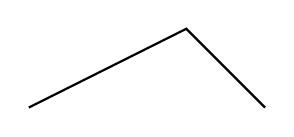
\begin{tikzpicture}
    \draw[thick] (0,0) to (2,1) to (3,0);
  \end{tikzpicture}
\] As time passes, the kink travels back and forth along the string,
being reflected at the ends. The beauty of this becomes apparent as we
watch the string right at the point where the bow is rubbing over it,
near the bottom end of the string. When the kink is between the bow and
the top end of the string: \[
  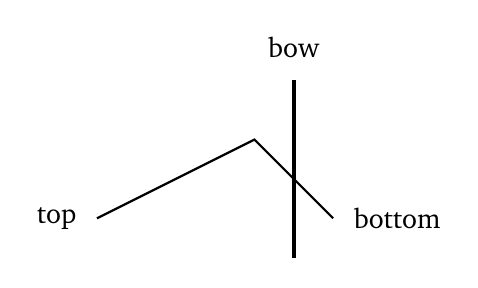
\begin{tikzpicture}
    \draw[thick] (0,0) node[label=left:{top}]{} to (2,1) to (3,0) node[label=right:{bottom}]{};
    \draw[ultra thick] (2.5,-0.5) to (2.5,1.75) node[label=above:{bow}]{};
  \end{tikzpicture}
\] this point in the string moves at the same speed and in the same
direction as the bow. This is called the ``sticking regime'', because
the static friction of the rosin-coated bow is enough to pull the string
along with it. But when the kink moves past the bow: \[
  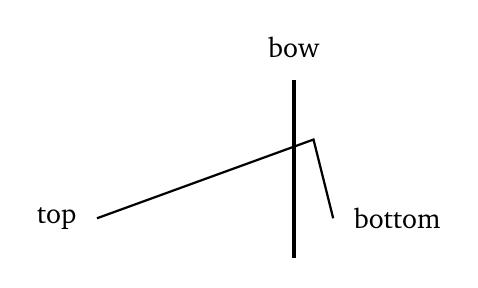
\begin{tikzpicture}
    \draw[thick] (0,0) node[label=left:{top}]{} to (2.75,1) to (3,0) node[label=right:{bottom}]{};
    \draw[ultra thick] (2.5,-0.5) to (2.5,1.75) node[label=above:{bow}]{};
  \end{tikzpicture}
\] the string slips off the bow and starts moving in the opposite
direction to it. This is called the ``sliding regime''. Since the
coefficient of sliding friction is less than the coefficient of static
friction, the string can slide against the motion of the bow in this
regime.

The really nice thing is that the string is vibrating almost freely: the
violinist just needs to apply the right amount of pressure to keep this
vibrational mode excited --- too much pressure will ruin it! Being able
to delicately control the Helmholtz waveform is part of what
distinguishes the virtuoso from the blood-curdling amateur.

The full physics of the violin is infinitely more complicated than this,
of course. The vibrating string excites the bridge which excites the
sound box, and \emph{that} produces most of the sound we hear. For more
information try these:

\begin{enumerate}
\def\labelenumi{\arabic{enumi})}
\setcounter{enumi}{1}
\item
  A. H. Benade, \emph{Fundamentals of Musical Acoustics}, Oxford
  University Press, Oxford, 1976.

  L. Cremer, \emph{The Physics of the Violin}, MIT Press, Cambridge,
  Massachusetts, 1984.

  N. H. Fletcher and T. D. Rossing, \emph{The Physics of Musical
  Instruments}, 2nd edition, Springer, New York, 1998.

  C. Hutchins and V. Benade, editors, \emph{Research Papers on Violin
  Acoustics 1975--1993}, 2 volumes, Acoustical Society of America, New
  York, 1997.
\end{enumerate}

Okay, now on to \(K(\mathbb{Z},2)\)! I explained a bit about this space
in \protect\hyperlink{week149}{``Week 149''}, but I've been pondering it
a lot lately, so I'd like to say a bit more.

First let me review and elaborate on some basic stuff I said already. If
G is any topological group, there is a topological space \(BG\) with a
basepoint such that the space of loops in \(BG\) starting and ending at
this point is homotopy equivalent to \(G\). This space \(BG\) is unique
up to homotopy equivalence. {[}\^{}1{]}

\(BG\) is important because it's the ``classifying space for
\(G\)-bundles''. What this means is that there's a principal
\(G\)-bundle over \(BG\) called the ``universal \(G\)-bundle'', with the
marvelous property that \emph{any} principal \(G\)-bundle over
\emph{any} space \(X\) is a pullback of this one by some map
\[f\colon X \to BG.\] (I explained in \protect\hyperlink{week149}{``Week
149''} how to pull back complex line bundles, and pulling back principal
\(G\)-bundles works the same way.) Even better, two \(G\)-bundles that
we get this way are isomorphic if and only if the maps they come from
are homotopic! So there is a one-to-one correspondence between:

\begin{enumerate}
\def\labelenumi{\Alph{enumi})}
\tightlist
\item
  isomorphism classes of principal \(G\)-bundles over \(X\)
\end{enumerate}

and

\begin{enumerate}
\def\labelenumi{\Alph{enumi})}
\setcounter{enumi}{1}
\tightlist
\item
  homotopy classes of maps from \(X\) to \(BG\).
\end{enumerate}

Now, suppose \(G\) is an \emph{abelian} topological group. Then \(BG\)
is better than a topological space with basepoint. It's an abelian
topological group!

This means that we can \emph{iterate} this trick. Starting with an
abelian topological group \(G\) we can form \(BG\), and \(BBG\), and
\(BBBG\), and so on. This is called ``delooping'', because the loop
space of each of these spaces is the previous one.

It's always fun to iterate any process whenever you can --- Freud called
this ``repetition compulsion'' --- but there's more going on here than
just that. In \protect\hyperlink{week149}{``Week 149''} I said that when
we have a list of spaces, each being the loop space of the previous one,
it's called a ``spectrum''. And I said that we can use a spectrum to get
a generalized cohomology theory. So we now have a trick for getting a
generalized cohomology theory from a topological abelian group!

In particular, suppose we start with a plain old abelian group \(A\). We
can think of it as a topological group with the discrete topology ---
let's call this \(K(A,0)\). Then we can define \[
  \begin{gathered}
    K(A,1) = B(K(A,0))
  \\K(A,2) = B(K(A,1))
  \\K(A,3) = B(K(A,2))
  \end{gathered}
\] \ldots{} and so on. We get a spectrum \(K(A,n)\) called an
``Eilenberg-MacLane spectrum''. The corresponding generalized cohomology
theory is just ordinary cohomology with coeffients in the abelian group
\(A\)! This means that \[H^n(X,A) = [X, K(A,n)]\] where the right-hand
side is the set of homotopy classes of maps from \(X\) to \(K(A,n)\). In
short, \(K(A,n)\) knows everything there is to know about the \(n\)th
cohomology with coefficients in \(A\).

We've seen this trick a couple of times lately, and it's actually a big
theme in homotopy theory: whenever we have some interesting invariant of
spaces, we try to cook up a space that ``represents'' this invariant. I
could say a LOT more about THIS idea, but that would propel us into
further heights of abstraction, when what I really want is to come down
to earth a bit. Just a little bit\ldots.

So: let's take \(A\) to be the integers, \(\mathbb{Z}\). As I said in
\protect\hyperlink{week149}{``Week 149''}, we then get
\[K(\mathbb{Z},0) = Z,\] \[K(\mathbb{Z},1) = \mathrm{U}(1),\] where
\(\mathrm{U}(1)\) is the group of ``phases'' or unit complex numbers,
and \[K(\mathbb{Z},2) = \mathbb{CP}^\infty\] where
\(\mathbb{CP}^\infty\) is infinite-dimensional complex projective space.
There are a couple of slightly different versions of this. Topologists
like to start with the direct limit of the spaces \(\mathbb{C}^n\),
which they call \(C^\infty\). Then they take the space of all
\(1\)-dimensional subspaces and call that \(\mathbb{CP}^\infty\).
Mathematical physicists prefer to start with a Hilbert space of
countable dimension. Then they take the space of unit vectors modulo
phase. Both these versions are equally good models of
\(K(\mathbb{Z},2)\). The first one is a lean, stripped-down version of
the second.

Now \(\mathrm{U}(1)\) is very important in quantum theory, and so are
unit vectors modulo phase in a Hilbert space --- physicists call these
``pure states''. So something cool is going on here. For some mysterious
reason, it looks like \(K(\mathbb{Z},n)\)'s are important quantum
physics! This is especially interesting because the abstract definition
of the \(K(\mathbb{Z},n)\)'s has nothing to do with the complex numbers
--- just the integers. The complex numbers show up on their own accord.
So maybe this hints at some explanation of why the complex numbers are
important in quantum mechanics.

Why are \(K(\mathbb{Z},n)\)'s connected to quantum theory? I don't
really know. But we can get some clues by asking some more specific
questions.

First of all, why is \(K(\mathbb{Z},2)\) the same as
\(\mathbb{CP}^\infty\)? In \protect\hyperlink{week149}{``Week 149''} I
just asserted this without proof. That's one of the fun things I'm
allowed to do in this column. But let me sketch why it's true.

First I need to remind you of some more basic facts about topology.
Suppose \(G\) is any topological group, and let \(P \to X\) be any
principal \(G\)-bundle. This gives us a long exact sequence of homotopy
groups:
\[\ldots \to \pi_{n+1}(X) \to \pi_n(G) \to \pi_n(P) \to \pi_n(X) \to \pi_{n-1}(G) \to \ldots\]
Two-thirds of the arrows in this sequence come from the maps
\[G \to P \to X\] while the less obvious remaining one-third come from
the map \[LX \to G\] sending each loop in the base space to the holonomy
of some connection on our bundle. Here \(LX\) means the space of based
loops in \(X\), and we're using the fact that
\[\pi_n(LX) = \pi_{n+1}(X)\] which is obvious from the definition of the
homotopy groups.

But now suppose \(P\) is contractible! Then all its homotopy groups
vanish, so the above long exact sequence breaks up into lots of puny
exact sequences like this: \[0 \to \pi_{n+1}(X) \to \pi_n(G) \to 0\] or
in other words: \[0 \to \pi_n(LX) \to \pi_n(G) \to 0\] This says that
the map from \(LX\) to \(G\) induces isomorphisms on all homotopy
groups. By the Whitehead theorem, this implies that this map is a
homotopy equivalence! So \(LX\) is really just \(G\)!! So \(X\) is just
\(BG\)!!!

In short: if we have a space \(X\) with a principal \(G\)-bundle \(P\)
over it, and \(P\) is contractible, \(X\) must be \(BG\). {[}\^{}2{]}

Now let's use this fact to show that \(\mathbb{CP}^\infty\) is
\(K(\mathbb{Z},2)\). Remember that by our recursive definition,
\[K(\mathbb{Z},2) = B(K(\mathbb{Z},1)) = B(\mathrm{U}(1))\] so to show
that \(\mathbb{CP}^\infty\) is \(K(\mathbb{Z},2)\), we just need to find
a principal \(\mathrm{U}(1)\)-bundle over it with a contractible total
space.

In \protect\hyperlink{week149}{``Week 149''} we discussed a complex line
bundle over \(\mathbb{CP}^\infty\) called the ``universal complex line
bundle''. If you take the space of unit vectors in a complex line bundle
you get a principal \(\mathrm{U}(1)\)-bundle. So let's do this to the
universal complex line bundle. What do we get? We get a principal
\(\mathrm{U}(1)\)-bundle like this: \[S^\infty \to \mathbb{CP}^\infty\]
Being a mathematical physicist, I'm using \(S^\infty\) here to stand for
the unit sphere in some countable-dimensional Hilbert space, and the map
sends each unit vector to the corresponding pure state, or unit vector
mod phase. Since there's a circle of unit vectors for each pure state,
this is indeed a principal \(\mathrm{U}(1)\)-bundle. But now for the
cool part: the unit sphere in an infinite-dimensional Hilbert space is
contractible! So we've got a principal \(\mathrm{U}(1)\)-bundle with a
contractible total space sitting over \(\mathbb{CP}^\infty\), proving
that \(\mathbb{CP}^\infty\) is \(K(\mathbb{Z},2)\). Even better, the
bundle \[S^\infty \to \mathbb{CP}^\infty\] is the universal principal
\(\mathrm{U}(1)\)-bundle.

I can't resist explaining why the unit sphere in an infinite-dimensional
Hilbert space is contractible. It seems very odd that a sphere could be
contractible, but this is one of those funny things about infinite
dimensions. Take our Hilbert space to be \(L^2[0,1]\) and consider any
function \(f\) in the unit sphere of this Hilbert space:
\[\int |f(x)|^2 dx = 1\] For \(t\) between \(0\) and \(1\), let
\(f_t(x)\) be a function that equals \(1\) for \(x < t\), and a sped-up
version of \(f\) for \(x\) greater than or equal to \(t\). If you do
this right \(f_t\) will still lie in the unit sphere, and you'll have a
way of contracting the whole unit sphere down to a single point, namely
the constant function \(1\).

Cute, huh?

Next question: how does \(\mathbb{CP}^\infty\) become an abelian
topological group? There's a very pretty answer. Consider the space of
rational functions of a single complex variable. This is a
infinite-dimensional complex vector space, and there's a natural way to
give it the topology of \(\mathbb{C}^\infty\). This gives us a nice way
to think of \(\mathbb{CP}^\infty\): it's just the \emph{nonzero}
rational functions modulo multiplication by constants.

But nonzero rational functions form an abelian group under
multiplication! And this is still true when we mod out by constant
factors! So \(\mathbb{CP}^\infty\) becomes an abelian group --- and in
fact an abelian topological group.

We can visualize \(\mathbb{CP}^\infty\) quite easily this way. A
rational function of a single complex variable has a bunch of zeros and
poles --- think of them as points on the Riemann sphere. We should
really stick an integer at each of these points: a positive integer at
each zero, and a negative integer at each pole, to tell us the order of
that zero or pole. This gives enough information to completely specify
the rational function up to a constant factor. So a point in
\(\mathbb{CP}^\infty\) is the same as a finite set of points on the
sphere labelled by integers --- which must add up to zero.

Of course, we have to get the right topology on \(\mathbb{CP}^\infty\).
As we move our point in \(\mathbb{CP}^\infty\) around in a continuous
way, the corresponding points on the sphere all move around
continuously, like a swarm of flies\ldots{} but when points collide,
their numbers add! For example, when a point labelled by the number 7
collides with a point labelled by the number -3, it turns into a point
labelled by the number \(7 - 3 = 4\).

In the lingo of physics, we've got a picture of points in
\(\mathbb{CP}^\infty\) as ``collections of particles and antiparticles
on the sphere''. The integer at any point on the sphere tells us the
number of particles sitting there --- but if it's negative, it means
we've got \emph{antiparticles} there. Particle-antiparticle pairs can be
created out of nothing, and they annihilate when they collide\ldots{}
it's very nice!

By the way, there's something called the Thom-Dold theorem that lets us
generalize the heck out of this. We just showed that if you take the
2-sphere and consider the space of particle-antiparticle swarms in it,
you get \(K(\mathbb{Z},2)\). But suppose instead we started with the
\(n\)-sphere and considered the space of particle-antiparticle swarms in
\emph{that}. Then we'd get \(K(\mathbb{Z},n)\)!

More generally, suppose we didn't use integers to say how many particles
were at each point in the \(n\)-sphere --- suppose we used elements of
some abelian group \(A\). Then we'd get \(K(A,n)\)!

For more tricks like this, try this paper:

\begin{enumerate}
\def\labelenumi{\arabic{enumi})}
\setcounter{enumi}{2}
\tightlist
\item
  Dusa McDuff, ``Configuration spaces of positive and negative
  particles'', \emph{Topology} \textbf{14} (1975), 91--107.
\end{enumerate}

Now let me mention a different picture of \(K(\mathbb{Z},2)\), that's
also nice, and also related to quantum theory. Take any
countable-dimensional Hilbert space \(H\) and let \(\mathrm{U}(H)\) be
the group of unitary operators on \(H\). Just like the unit sphere in
this Hilbert space is contractible, it turns out that \(\mathrm{U}(H)\)
is contractible if we give it the norm topology or the strong topology.

Anyway, now let \(\mathrm{PU}(H)\) be the ``projective unitary group''
of \(H\), meaning the group of unitary operators modulo phase. There's
an obvious map \[\mathrm{U}(H) \to \mathrm{PU}(H)\] sending a circle's
worth of points to each point in \(\mathrm{PU}(H)\). It's easy to check
that this is a principal \(\mathrm{U}(1)\)-bundle. Since the total space
\(\mathrm{U}(H)\) is contractible, it follows that \(\mathrm{PU}(H)\) is
\(K(\mathbb{Z},2)\)!

This give a \emph{nonabelian} group structure on \(K(\mathbb{Z},2)\),
which may seem kind of weird, given that we just made it into an
\emph{abelian} group a minute ago. But I guess this other product is
``abelian up to homotopy'' in a very strong sense, so it's just as good
as abelian for the purposes of homotopy theory.

Anyway, some people in Australia have figured out an extra trick you can
do with this \(\mathrm{PU}(H)\) group:

\begin{enumerate}
\def\labelenumi{\arabic{enumi})}
\setcounter{enumi}{3}
\tightlist
\item
  Alan L. Carey, Diarmuid Crowley and Michael K. Murray, ``Principal
  bundles and the Dixmier-Douady class'', \emph{Comm. Math. Physics}
  \textbf{193} (1998) 171--196, preprint available as
  \href{https://arxiv.org/abs/hep-th/9702147}{\texttt{hep-th/9702147}}.
\end{enumerate}

Here's how it goes, at least in part. We say a linear operator
\[A\colon H \to H\] is ``Hilbert-Schmidt'' if the trace of \(AA^*\) is
finite. The space of Hilbert-Schmidt operators is a Hilbert space in its
own right, with this inner product:
\[\langle A,B\rangle = \operatorname{tr}(AB^*)\] Let's call this Hilbert
space \(X\). \(\mathrm{U}(H)\) acts on \(X\) by conjugation, and this
gives an action of \(\mathrm{PU}(H)\) on \(X\), because phases commute
with everything. This in turn gives an action of \(\mathrm{PU}(H)\) on
\(\mathrm{U}(X)\)! Is your brain melting yet? Anyway, it turns out that
this makes \(\mathrm{U}(X)\) into the total space of a principal
\(\mathrm{PU}(H)\)-bundle:
\[\mathrm{PU}(H) \to \mathrm{U}(X) \to \mathrm{U}(X)/\mathrm{PU}(H)\]
But \(X\) is a countable-dimensional Hilbert space, so \(\mathrm{U}(X)\)
is contractible, so this is the \emph{universal} principal
\(\mathrm{PU}(H)-bundle\). And as we've seen, this means that
\[\mathrm{U}(X)/\mathrm{PU}(H) = B(\mathrm{PU}(H))\] but we just saw
that \[\mathrm{PU}(H) = K(\mathbb{Z},2)\] so
\[\mathrm{U}(X)/\mathrm{PU}(H) = B(\mathrm{PU}(H)) = B(K(\mathbb{Z},2)) = K(\mathbb{Z},3) \,\text{!}\]

In \protect\hyperlink{week149}{``Week 149''}, I said I'd like
\(K(\mathbb{Z},3)\) to be some sort of infinite-dimensional manifold
closely related to quantum physics. I'm happier now, because here we are
getting just that --- technically, we're getting it to be a ``Banach
manifold''. Of course, I could still complain that this description
doesn't make the \emph{abelian group structure} on \(K(\mathbb{Z},3)\)
obvious. But it's definitely a big step towards understanding what
\(K(\mathbb{Z},n)\)'s have to do with quantum theory.

While I'm at it, I should report some other things people have told me
via email. If you ponder what I've said, you can see that
\(\mathbb{CP}^\infty\) has 2nd homology equal to \(\mathbb{Z}\), and
that the generator of this homology group --- the ``universal cycle''
--- is given geometrically by the obvious way of sticking the sphere
\(\mathbb{CP}^1\) inside \(\mathbb{CP}^\infty\). This is nice because
\(\mathbb{CP}^1\) is actually a submanifold of the manifold
\(\mathbb{CP}^\infty\). But according to email from Mark Goresky, Rene
Thom has shown that for \(n > 6\), we cannot make \(K(\mathbb{Z},n)\)
into a manifold in such a way that the universal cycle is represented by
a submanifold!

On the other hand, Michael Murray reports that Pawel Gajer has managed
to make \(K(\mathbb{Z},n)\) into something called a ``differential
space'', which is not quite a manifold, but good enough to do geometry
on. I'm not sure how this relates to Thom's work\ldots{} but anyway, I
should read this stuff:

\begin{enumerate}
\def\labelenumi{\arabic{enumi})}
\setcounter{enumi}{4}
\item
  Pawel Gajer, ``Geometry of Deligne cohomology'', \emph{Invent. Math.}
  \textbf{127} (1997), 155--207, also available as
  \href{https://arxiv.org/abs/alg-geom/9601025}{\texttt{alg-geom/9601025}}.

  Pawel Gajer, ``Higher holonomies, geometric loop groups and smooth
  Deligne cohomology'', \emph{Advances in Geometry}, Birkhauser, Boston,
  1999, pp.~195--235.
\end{enumerate}

Now, so far I've been restraining myself from talking about ``gerbes'',
but if you've gotten this far you must be pretty comfortable with
abstract nonsense, so you'll probably like gerbes. Very roughly
speaking, a gerbe is a categorified version of a principal bundle!
Actually it's a categorified version of a sheaf, but sometimes we can
think of it as analogous to the sheaf of sections of a bundle. And just
as \(K(\mathbb{Z},2)\) is the classifying space for \(\mathrm{U}(1)\)
bundles, \(K(\mathbb{Z},3)\) is the classifying space for a certain sort
of gerbe!

I sort of explained how this works in \protect\hyperlink{week25}{``Week
25''}, but you can read the details here:

\begin{enumerate}
\def\labelenumi{\arabic{enumi})}
\setcounter{enumi}{5}
\tightlist
\item
  Jean-Luc Brylinski, \emph{Loop Spaces, Characteristic Classes and
  Geometric Quantization}, Birkhauser, Boston, 1993.
\end{enumerate}

What this means is that as we explore the meaning of these
\(K(\mathbb{Z},n)\)'s for quantum theory, we are really
\emph{categorifying} familiar ideas from quantum theory. In particular,
this story should keep going on forever: \(K(\mathbb{Z},4)\) should be
the classifying space for a certain sort of 2-gerbe, and so on. But I
don't think people have worked out the details beyond the case of
2-gerbes. If you want to learn about 2-gerbes, you have to read this:

\begin{enumerate}
\def\labelenumi{\arabic{enumi})}
\setcounter{enumi}{6}
\tightlist
\item
  Lawrence Breen, ``On the Classification of 2-Gerbes and 2-Stacks'',
  \emph{Asterisque} \textbf{225}, 1994.
\end{enumerate}

Finally, for more applications to physics, try these papers:

\begin{enumerate}
\def\labelenumi{\arabic{enumi})}
\setcounter{enumi}{7}
\item
  Alan L. Carey and Michael K. Murray, ``Faddeev's anomaly and bundle
  gerbes'', \emph{Lett. Math. Phys.} \textbf{37} (1996), 29--36.

  Jouko Mickelsson, ``Gerbes and Hamiltonian quantization of chiral
  fermions'', in \emph{Lie Theory and Its Applications in Physics},
  World Scientific, Singapore, 1996, pp.~216--225.

  Michael K. Murray, ``Bundle gerbes'', \emph{J. London Math. Soc.}
  \textbf{54} (1996), 403--416.

  Alan L. Carey, Jouko Mickelsson and Michael K. Murray, ``Index theory,
  gerbes, and Hamiltonian quantization'', \emph{Comm. Math. Phys.}
  \textbf{183} (1997), 707--722, preprint available as
  \href{https://arxiv.org/abs/hep-th/9511151}{\texttt{hep-th/9511151}}.

  Alan L. Carey, Michael K. Murray and B. L. Wang, ``Higher bundle
  gerbes and cohomology classes in gauge theories'', \emph{J. Geom.
  Phys.} \textbf{21} (1997) 183--197, preprint available as
  \href{https://arxiv.org/abs/hep-th/9511169}{\texttt{hep-th/9511169}}.

  Alan L. Carey, Jouko Mickelsson and Michael K. Murray, ``Bundle gerbes
  applied to quantum field theory'', \emph{Rev.~Math. Phys.} \textbf{12}
  (2000), 65--90, preprint available as
  \href{https://arxiv.org/abs/hep-th/9711133}{\texttt{hep-th/9711133}}.
\end{enumerate}

I thank N. Christopher Phillips of the University of Oregon, Michael K.
Murray and Diarmuid Crowley of the University of Adelaide, and Mark
Goresky of IHES for educating me about these matters\ldots{} all
remaining errors are mine!

\begin{center}\rule{0.5\linewidth}{0.5pt}\end{center}

{[}\^{}1{]} I'm being sloppy here. Throughout this discussion, when I
say ``homotopy equivalent'', I really mean ``weakly homotopy
equivalent'' --- a technical nuance that you can read about in any good
book on homotopy theory.

{[}\^{}2{]} Moreover, \(P\) must be the universal principal
\(G\)-bundle. Conversely, for any topological group \(G\) the total
space of the universal principal \(G\)-bundle is contractible.
Everything fits together very neatly! But I don't need all this stuff
now.



\hypertarget{week152}{%
\section{July 5, 2000}\label{week152}}

I've been reading about the mathematical physicist William Rowan
Hamilton lately, because I'm writing a review article about the
octonions --- that famous nonassociative \(8\)-dimensional division
algebra.

You see, the day after Hamilton discovered the quaternions and carved
the crucial formula \[i^2=j^2=k^2=ijk=-1\] on the Brougham bridge, he
mailed a letter explaining his discovery to his friend John Graves. And
about two months later, Graves discovered the octonions! In December
1843, he sent a letter about them to Hamilton.

Graves called them ``octaves'' at first, but later introduced the term
``octonions''. He showed they were a normed division algebra and used
this to prove the 8 squares theorem, which says that the product of two
sums of 8 perfect squares is again a sum of 8 perfect squares. The
complex numbers and quaternions allow one to prove similar theorems for
2 and 4 squares. In January 1844, Graves considered the idea of a
general theory of ``\(2^m\)-ions''. He tried to construct a
\(16\)-dimensional normed division algebra and use it to prove a 16
squares theorem, but he ``met with an unexpected hitch'' and came to
doubt that this was possible.

(If you read \protect\hyperlink{week59}{``Week 59''} you'll see why.)

Hamilton was the one who noticed that the octonions were nonassociative
--- in fact, he invented the word ``associative'' right about this time.
He offered to write a paper publicizing Graves' work, and Graves
accepted the offer, but Hamilton kept putting it off. He was probably
busy working on the quaternions!

Meanwhile, Arthur Cayley had heard about the quaternions right when
Hamilton announced his discovery, and he eventually discovered the
octonions on his own. He published a description of them in the March
1845 issue of the Philosophical Magazine. Graves was upset, so he added
a postscript about the octonions to a paper of his that was due to
appear in the following issue of the same journal, asserting that he'd
known about them since Christmas 1843. Also, Hamilton eventually got his
act together and published a short note about Graves' discovery in the
June 1847 issue of the Proceedings of the Royal Irish Academy. But by
then it was too late --- everyone was calling the octonions ``Cayley
numbers''.

Of course it wasn't \emph{really} too late, since everybody who cares
can now tell that Graves was the first to discover the octonions. And
anyway, it doesn't really make a difference who discovered them first,
except as a matter of historical interest.

But just for the heck of it, I'm trying to find out everything I can
about the early history of the octonions. Hamilton is very famous, and
much has been written about him, but Graves is mainly famous for being
Hamilton's friend --- so to learn stuff about Graves, I have to read
books on Hamilton. In the process, I've learned some interesting things
that aren't really relevant to my review article. And I want to tell you
about some of them before I forget!

Hamilton was a strangely dreamy sort of guy. He spent most of his life
as the head of a small observatory near Dublin, but quickly lost
interest in actually staying up nights to make observations. Instead, he
preferred writing poetry. He was friends with Coleridge, who introduced
him to the philosophy of Kant, which influenced him greatly. He was also
friends with Wordsworth --- who told him to not to write poetry. He fell
deeply in love with a woman named Catherine Disney, who was forced by
her parents to marry a wealthy man 15 years older than her. Hamilton
remained hopelessly in love with her the rest of his life, though he
eventually married someone else. He became an alcoholic, then foreswore
drink, then relapsed. Eventually, many years later, Catherine began a
secret correspondence with him --- she still loved him! Her husband
became suspicious, she attempted suicide by taking laudanum\ldots{} and
then, five years later, she became ill.~Hamilton visited her and gave
her a copy of his ``Lectures on Quaternions'' --- they kissed at long
last --- and then she died two weeks later. He carried her picture with
him ever afterwards and talked about her to anyone who would listen. A
very sad and very Victorian tale.

He was a bit too far ahead of his time to have maximum impact during his
own life. The Hamiltonian approach to mechanics and the Hamilton-Jacobi
equation relating waves and particles became really important only when
quantum mechanics came along. Luckily Klein liked this stuff, and told
Schroedinger about it. But it's a pity that Hamilton's unification of
particle and wave mechanics came along right when the advocates of the
wave theory of light seemed to have definitively won the battle against
the particle theory --- the need for a compromise became clear only
later.

Quaternions, too, might have had more impact if they'd come along later,
when people were trying to understand spin-\(1/2\) particles. After all,
the unit quaternions form the group \(\mathrm{SU}(2)\), which is perfect
for studying spin-\(1/2\) particles. But the way things actually went,
quaternions were not very popular by the time people dreamt of
spin-\(1/2\) particles --- so Pauli just used \(2\times\) complex
matrices to describe the generators of \(\mathrm{SU}(2)\).

I like what Hamilton wrote about quaternions, space, and time:

\begin{quote}
The quaternion was born, as a curious offspring of a quaternion of
parents, say of geometry, algebra, metaphysics, and poetry\ldots{} I
have never been able to give a clearer statement of their nature and
their aim than I have done in two lines of a sonnet addressed to Sir
John Herschel:

\begin{quote}
\begin{verbatim}
           "And how the One of Time, of Space the Three
            Might in the Chain of Symbols girdled be."
\end{verbatim}
\end{quote}
\end{quote}

It's also amusing how Hamilton responded when de Morgan told him about
the four-color conjecture: ``I am not likely to attempt your `quaternion
of colours' very soon.'' The pun is ironic, given the relations people
have recently discovered between what is now the four-color theorem, the
vector cross product, and the group \(\mathrm{SU}(2)\). (See
\protect\hyperlink{week8}{``Week 8''} and
\protect\hyperlink{week92}{``Week 92''} for more.)

Of course quaternions were very influential for a while --- they were
taught in many mathematics departments in America in the late 1800s, and
were even a mandatory topic of study at Dublin! But then they were
driven out by the vector notation of Gibbs and Heaviside. If you don't
know this story, you've got to read this book --- it's fascinating:

\begin{enumerate}
\def\labelenumi{\arabic{enumi})}
\tightlist
\item
  Michael J. Crowe, \emph{A History of Vector Analysis}, University of
  Notre Dame Press, Notre Dame, 1967.
\end{enumerate}

Check out the graphs showing how many books were written on quaternions:
the big boom in the 1860s, and then the bust!

I hadn't even known about what many people at the time considered
Hamilton's greatest achievement: the prediction of ``conical
refraction'' by a biaxial crystal like aragonite. Folks compared this to
the discovery of Neptune by Adams and Leverrier --- another triumph of
prediction --- and Hamilton won a knighthood for it.

Does anyone understand how this phenomenon works? I don't.

Personally, I think one of Hamilton's greatest triumphs was his
treatment of complex numbers as pairs of real numbers --- this finally
exorcised the long-standing fears about whether imaginary numbers
``really exist'', and helped opened up the way for other algebras.
Interestingly, the person who got him interested in this problem was
John Graves. Graves was the one who introduced Hamilton to John Warren's
book ``A Treatise on the Geometrical Representation of the Square Root
of Negative Quantities'', which explained the concept of the complex
plane. Hamilton turned this from geometry into algebra.

One of Hamilton's last inventions was the icosian calculus. Faithful
fans of This Week's Finds will remember the icosians from
\protect\hyperlink{week20}{``Week 20''}. These were invented by Conway
and Sloane; Hamilton's original icosian calculus was a bit different. In
August 1856, Hamilton went to the British Association Meeting at
Cheltenham and stayed at the house of his pal John Graves. He enjoyed
talking to Graves and reading his books: ``Conceive me shut up and
revelling for a fortnight in John Graves' Paradise of Books! of which he
has really an astonishingly extensive collection, especially in the
curious and mathematical kinds. Such new works from the Continent he has
picked up! and such rare old ones too!'' Graves posed some puzzles to
Hamilton, and either Graves or his books got Hamilton to thinking about
regular polyhedra. When Hamilton returned to Dublin he thought about the
symmetry group of the icosahedron, and used it to invent an algebra he
called the ``icosians''. He then sent a letter to Graves explaining the
icosians.

He basically said: assume we've got three symbols \(I\), \(K\), and
\(L\) satisfying these relations:
\[I^2 = 1,\quad K^3 = 1,\quad L^5 = 1,\quad L = IK \] together with the
associative law but not the commutative law. You can think of \(L\) as
corresponding to rotating an icosahedron \(1/5\) of a turn around a
vertex. \(K\) corresponds to rotating it \(1/3\) of a turn around a
face, and \(I\) corresponds to rotating it \(1/2\) of a turn around an
edge. The relations above all follow from this idea.

These days, we would call the icosians the ``group algebra of \(A_5\)''.
In modern lingo, the symmetry group of the icosahedron is called
\(A_5\), since it's the group of all even permutations of 5 things. If
you don't know why this is true, check this out:

\begin{enumerate}
\def\labelenumi{\arabic{enumi})}
\setcounter{enumi}{1}
\tightlist
\item
  John Baez, ``Some thoughts on the number six'',
  \texttt{http://math.ucr.edu/home/baez/six.html}
\end{enumerate}

We form the ``group algebra'' of a group by taking all formal linear
combinations of group elements with real coefficients, and defining a
product of such combinations using the product in the group. The
dimension of a group algebra is just the number of elements in the
group. Since \(A_5\) has 60 elements, the icosians are a 60-dimensional
algebra. These days this stuff is no big deal. But back then, I bet a
60-dimensional noncommutative algebra was really mindblowing!

In a way that I don't fully understand, Hamilton connected the icosian
calculus to the problem of travelling along the edges of a dodecahedron,
hitting each vertex just once, and coming back to where you started. In
graph theory, this sort of thing is now called a ``Hamiltonian
circuit''. Hamilton even invented a puzzle where the first player takes
the first five steps any way they want, and the other player has to
complete the Hamiltonian circuit. He called this the ``icosian game''.

It was John Graves' idea to actually design a game board with the
dodecahedron graph drawn on it and holes at the vertices that you could
put small cylindrical markers into. In 1859, a friend of Graves
manufactured a version where the game board had legs like a small table,
and sent a copy to Hamilton. Naturally Hamilton was delighted! Graves
put Hamilton in contact with a London toymaker named John Jacques, and
Hamilton sold Jacques the rights to the game for 25 pounds and 6 copies.
Jacques marketed two versions, one for the parlor, which was played on a
flat board, and another for the ``traveler'', which was played on an
actual dodecahedron --- there was a nail at each vertex, and the players
wound string about these nails as they traced out their Hamiltonian
circuit.

With charming naivete, Hamilton had hopes that the game would sell
wildly. Alas, it did not. Jacques never even recouped his investment.
The problem was that the icosian game was too easy, even for children!
Amusingly, Hamilton had more trouble with it than most people ---
perhaps because he was using the icosian calculus to figure out his
moves, instead of just trying different paths.

By the way, if anyone knows any good source of information about Graves
or the invention of the octonions, I'd love to hear about it. So far
I've gotten most of my stuff from the following sources. First of all,
there's this nice biography of Hamilton:

\begin{enumerate}
\def\labelenumi{\arabic{enumi})}
\setcounter{enumi}{2}
\tightlist
\item
  Thomas L. Hankins, \emph{Sir William Rowan Hamilton}, John Hopkins
  University Press, Baltimore, 1980.
\end{enumerate}

Check out the picture of the icosian game on page 342!

Then there's this much longer biography, which includes lots of
correspondence:

\begin{enumerate}
\def\labelenumi{\arabic{enumi})}
\setcounter{enumi}{3}
\tightlist
\item
  Robert Perceval Graves, \emph{Life of Sir William Rowan Hamilton}, 3
  volumes, Arno Press, New York 1975.
\end{enumerate}

Robert Perceval Graves was the brother of John Graves! He idolized
Hamilton, so this is not the most balanced account of his work.

Then there is this very helpful summary of the Hamilton-Graves
correspondence on octonions:

\begin{enumerate}
\def\labelenumi{\arabic{enumi})}
\setcounter{enumi}{4}
\tightlist
\item
  W. R. Hamilton, ``Four and eight square theorems'', Appendix 3 of
  vol.~III of \emph{The Mathematical Papers of William Rowan Hamilton},
  eds.~H. Halberstam and R. E. Ingram, Cambridge University Press,
  Cambridge, 1967.
\end{enumerate}

Unfortunately this does not include Graves' first letter to Hamilton
about the octonions. Is it lost?

Finally, there's this history of later work on the octonions and the
eight square theorem:

\begin{enumerate}
\def\labelenumi{\arabic{enumi})}
\setcounter{enumi}{5}
\tightlist
\item
  L. E. Dickson, ``On quaternions and their generalization and the
  history of the eight square theorem'', \emph{Ann. Math.} \textbf{20}
  (1919), 155--171.
\end{enumerate}

It turns out the eight square theorem was proved in 1822, before Graves.
Also, there's some good material in here:

\begin{enumerate}
\def\labelenumi{\arabic{enumi})}
\setcounter{enumi}{6}
\tightlist
\item
  Heinz-Dieter Ebbinghaus et al, \emph{Numbers}, Springer, New York,
  1990.
\end{enumerate}

This book is a lot of fun for anyone interested in all sorts of
``numbers''.

Finally, for an excellent \emph{online} source of information on the
history of quaternions, octonions, and other ``hypercomplex number
systems'', this is the place to go:

\begin{enumerate}
\def\labelenumi{\arabic{enumi})}
\setcounter{enumi}{7}
\tightlist
\item
  Jeff Biggus, ``A history of hypercomplex numbers'',
  \texttt{http://history.hyperjeff.net/hypercomplex.html}
\end{enumerate}

\begin{center}\rule{0.5\linewidth}{0.5pt}\end{center}

\textbf{Addendum:} On April 14th, 2005 I received the following email
from Geoff Corbishley in response to my plea for more information about
John Graves:

\begin{quote}
John

Your page asks for information on John Graves. I am reading
\emph{Goodbye to all That}, the autobiography of Robert Graves who also
wrote \emph{I Claudius} and other books. Chapter 1 (page 14 in my
Penguin paperback) records that John Thomas Graves helped WR Hamilton
with quaternions and gives a list of other relatives. Very little extra
detail is given about JT Graves, sadly.

Hope that has not been reported too often\ldots.

Geoff
\end{quote}

Fans of Hamilton might like to see my webpage with photos of the plaque
on Brougham Bridge commemorating his discovery of the quaternions:

\begin{enumerate}
\def\labelenumi{\arabic{enumi})}
\setcounter{enumi}{8}
\tightlist
\item
  John Baez, Brougham Bridge,
  \texttt{http://math.ucr.edu/home/baez/octonions/node24.html}
\end{enumerate}



\hypertarget{week153}{%
\section{July 15, 2000}\label{week153}}

This one is going to be a bit rough at the edges, because in a few hours
I'm taking a plane to London. I'm going to the International Congress on
Mathematical Physics, where I'll get to hear talks by Ashtekar, Atiyah,
Buchholz, Connes, Dijkgraaf, Donaldson, Faddeev, Freed, Froehlich,
Kreimer, Ruelle, Schwartz, Shor, Thirring, 't Hooft, and other
math/physics heavyweights. I'm also gonna talk a bit myself --- they'd
have to pay me to shut up! I hope to report on this stuff in future
issues.

But today, I want to say a bit about counting.

Archimedes loved to count. In his Sand Reckoner, he invented a notation
for enormous numbers going far beyond what the Greeks had previously
considered. He made up a nice problem to showcase these large numbers:
how many grains of sand would it take to fill the universe? He then
computed an upper bound, based on assumptions such as these:

\begin{enumerate}
\def\labelenumi{\Alph{enumi})}
\item
  No more than 10,000 grains of sand can fit into a sphere whose
  diameter was \(1/40\)th a finger-width.
\item
  The circumference of the earth is no more than 3,000,000 stades. A
  ``stade'' is about 160 meters --- different Greek cities used
  different stades, so it difficult to be very precise about this.
\item
  The diameter of the earth is greater than the diameter of the moon.
\item
  The diameter of the sun is no more than 30 times the diameter of the
  moon. (Of course this one is way off!)
\item
  The diameter of the sun is greater than the side of a regular
  chiliagon inscribed in a great circle in the sphere of the universe. A
  chiliagon is a thousand-sided polygon.
\end{enumerate}

He concluded that no more than \(10^{63}\) grains of sand would be
needed to fill the universe. Of course, he didn't use modern exponential
notation! Instead, he used a system of his own devising. The largest
number the Greeks had a notation for was a ``myriad myriads'', or
\(10^8\), since a ``myriad'' means 10,000. Archimedes called \(10^8\) a
number of the ``first order''. He then invented a number of the ``second
order'', namely \(10^{16}\), and the ``third order'', namely \(10^{24}\)
--- and so on, up to the myriad-myriadth order, i.e.~\(10^8\) to the
\(10^8\)th power.

He then said all these numbers were of the ``first period'', and went on
to define higher periods of numbers, up to a number of the myriadth
period, which was \(10^{80,000,000,000,000,000}\). After this exercise,
the number of grains of sand in the universe must have seemed rather
puny --- merely a thousand myriads of numbers of the eighth order!

Actually, this counting exercise is one of Archimedes' lesser feats. He
pioneered many of the concepts of mechanics and calculus. He also had
the neat idea to use mechanical methods to do calculations and ``prove
theorems''. He wrote about this in a treatise called ``Methods of
Mechanical Theorems''. There is only one surviving copy of this
treatise, and that is a fascinating story in itself. It is part of the
``Archimedes Palimpsest'', a copy of various works of Archimedes which
dates back to the 10th century A.D.. A ``palimpsest'' is a parchment
which was reused and written over --- in this case, by Greek monks. The
Archimedes palimpsest has a long and complicated history, and only in
1998 was it made publicly accessible at the Walters Art Gallery. For
more on this, see:

\begin{enumerate}
\def\labelenumi{\arabic{enumi})}
\item
  Reviel Netz, ``The origins of mathematical physics: new light on an
  old question'', \emph{Physics Today}, June 2000, 32--37.
\item
  The Walters Art Gallery, Archimedes Palimpsest website,
  \texttt{http://www.thewalters.org/archimedes/frame.html}
\end{enumerate}

For more on Archimedes, try:

\begin{enumerate}
\def\labelenumi{\arabic{enumi})}
\setcounter{enumi}{2}
\tightlist
\item
  Chris Rorres, Archimedes website,
  \texttt{http://www.mcs.drexel.edu/\textasciitilde{}crorres/Archimedes/contents.html}
\end{enumerate}

Anyway, back to counting. These days I'm interested in generalizations
of ``cardinality''. The cardinality of a set S is just its number of
elements, which I'll denote by \(|S|\). The great thing about this is
that if you know the cardinality of a set, you know that set up to
isomorphism: any two sets with the same number of elements are
isomorphic. Of course, this is no coincidence: it's exactly what numbers
were invented for!

I explained this using the ``parable of the shepherd'' in
\protect\hyperlink{week121}{``Week 121''}, so I won't run through that
spiel again. Instead, I'll just remind you of the basic facts: there's a
category \(\mathsf{FinSet}\) whose objects are finite sets and whose
morphisms are functions. We can ``decategorify'' any category by forming
the set of isomorphism classes of objects. When we do this to
\(\mathsf{FinSet}\) we get the set of natural numbers, \(\mathbb{N}\).
So given any finite set \(S\), its isomorphism class \(|S|\) is just a
natural number --- its cardinality!

Via this trick the natural numbers inherit all their basic operations
from corresponding operations in \(\mathsf{FinSet}\). For example, given
two finite sets \(S\) and \(T\) we can form their disjoint union
\(S + T\) and their Cartesian product, and these operations give birth
to addition and multiplication of natural numbers, via these formulas:
\[
  \begin{aligned}
    |S + T| &= |S| + |T|
  \\|S \times T| &= |S| \times |T|
  \end{aligned}
\] Now the advantage of this rather esoteric view of basic arithmetic is
that it suggests vast generalizations which unify all sorts of seemingly
disparate stuff. For example, we can play this ``decategorification''
game to categories other than \(\mathsf{FinSet}\). For example, we can
do it to the category \(\mathsf{Vect}\) whose objects are vector spaces
and whose morphisms are linear functions --- and what do we get? The set
\(\mathbb{N}\) again! But this time we don't call the isomorphism class
of a vector space its ``cardinality'' --- we call it the ``dimension''.
And this time, addition and multiplication of natural numbers correspond
to direct sum and tensor product of vector spaces.

Well, this example is so familiar that it may seem that we're still not
getting anywhere interesting. But suppose we consider the category of
\(\mathsf{Vect}(X)\) of vector \emph{bundles} over a topological space
\(X\). If we take X to be a single point this is just \(\mathsf{Vect}\)
--- a vector bundle over a point is a vector space. But if we take \(X\)
to be more interesting, when we decategorify \(\mathsf{Vect}(X)\) we get
an interesting set that depends on \(X\). Since we can take direct sums
and tensor products of vector bundles, this set has addition and
multiplication operations. Like the natural numbers, this set is not a
ring, since it doesn't have additive inverses. It's a mere ``rig'' --- a
``ring without negatives''.

But just as we created the integers by making up additive inverses for
the natural numbers, we can take this set and throw in formal additive
inverses to get a ring. What ring do we get? Well, it depends on \(X\):
it's called the ``K-theory of \(X\)'', and denoted \(K(X)\). Studying
this ring \(K(X)\) is a wonderful way to understand the space \(X\).
K-theory is a great example of a generalized cohomology theory (see
\protect\hyperlink{week149}{``Week 149''} and
\protect\hyperlink{week150}{``Week 150''}). To explain it in detail
would require a book. Luckily, such books already exist. In fact there
are a bunch! Here are 3 of my favorites:

\begin{enumerate}
\def\labelenumi{\arabic{enumi})}
\setcounter{enumi}{3}
\item
  Raoul Bott, \emph{Lectures on K(X)}, Harvard University, Cambridge,
  1963.
\item
  Michael Atiyah, \emph{K-theory}, W. A. Benjamin, New York, 1967.
\item
  Max Karoubi, \emph{K-theory: an Introduction}, Springer, Berlin, 1978.
\end{enumerate}

There are a million variations on this decategorification trick: for
example, we can decategorify the category of complex line bundles on the
space \(X\), and get a set called \(H^2(X)\) --- the ``second cohomology
group of \(X\)''. This is an abelian group thanks to the fact that we
can take tensor products of line bundles. The isomorphism class of any
complex line bundle gives an element of \(H^2(X)\) called the ``first
Chern class'' of the line bundle. For more about this see
\protect\hyperlink{week149}{``Week 149''}\ldots. my point here is that
this is just a generalization of the idea of cardinality!

Or, we can start with the category of finite-dimensional representations
of a group \(G\). When we decategorify this we get a rig, since we can
take direct sums and tensor products of representations. If we throw in
additive inverses, we get a ring \(R(G)\) called the ``representation
ring'' of \(G\). The isomorphism class of any representation gives an
element of \(R(G)\) which people call the ``character'' of that
representation.

Or start with the category where an object is an action of \(G\) on a
finite set! Decategorifying and then throwing in additive inverses, we
get something called the ``Burnside ring'' of \(G\).

In fact, the last two examples are special cases of something more
general: we can start with the category
\(\operatorname{Hom}(G,\mathcal{C})\) where the objects are actions of
\(G\) on objects in some category \(\mathcal{C}\)! Different choices of
\(\mathcal{C}\) give different views of the group \(G\), and different
structures on \(\mathcal{C}\) will give us a group, or a rig, when we
decategorify \(\operatorname{Hom}(G,\mathcal{C})\). I am tempted to
launch into a detailed disquisition on how this works, but I fear such
generality will exhaust the patience of all but the true lovers of
abstraction --- who can figure it out for themselves anyway! So let me
descend earthwards a few hundred meters and let the winds hasten me
towards my ultimate goal, which is\ldots{} elliptic cohomology.

Suppose we decategorify the category of compact oriented smooth
manifolds! What are the morphisms in this category? Well, let's take
them to be cobordisms. And to simplify life let's throw in formal
inverses to all these morphisms, so manifolds with a cobordism between
them get counted as isomorphic. We get a category where all the
morphisms are isomorphisms. And when decategorify this, we get a big
set. This set becomes a rig thanks to our ability to take disjoint
unions and Cartesian products of compact oriented smooth manifolds. In
fact it's a ring, because the orientation-reversed version of any
manifold serves as its additive inverse. This ring is obviously
commutative. People call it the ``oriented cobordism ring''. And believe
or not, people know quite a bit about this ring.

To simplify this ring a bit, let's tensor it with the complex numbers.
We get an algebra that's easy to describe: it's just the algebra of
complex polynomials in countably many variables! These variables
correspond to the complex projective spaces \(\mathbb{CP}^2\),
\(\mathbb{CP}^4\), \(\mathbb{CP}^6,\) etcetera --- so folks sometimes
write this algebra as follows:
\[\mathbb{C}[\mathbb{CP}^2,\mathbb{CP}^4,\mathbb{CP}^6,\ldots]\] Now,
using this algebra we can cook up various notions analogous to the
``cardinality'' of a compact oriented smooth manifold. But people don't
say ``cardinality'', they say ``genus''. Don't be fooled --- if you know
about the genus of a surface, this isn't that! In this definition, a
``genus'' assigns to each compact oriented manifold \(M\) a complex
number \(|M|\) such that \[
  \begin{aligned}
    |M + N| &= |M| + |N|
  \\|M \times N| &= |M| \times |N|
  \end{aligned}
\] and \(|M| = |M'|\) if there is a cobordism from \(M\) to \(M'\). If
you stare at this definition carefully, you'll see that a genus is
really just a homomorphism from
\(\mathbb{C}[\mathbb{CP}^2,\mathbb{CP}^4,\mathbb{CP}^6,\ldots]\) to the
complex numbers.

As any classicist will tell you, the plural of genus is ``genera''.
Examples of genera include the signature and \(\hat{A}\) genus, both
beloved by topologists and differential geometers. The Euler
characteristic is \emph{not} a genus since it is not cobordism invariant
--- very much a pity, since it's so much like the cardinality in so many
ways (see \protect\hyperlink{week146}{``Week 146''}.)

Since the algebra
\(\mathbb{C}[\mathbb{CP}^2,\mathbb{CP}^4,\mathbb{CP}^6,\ldots]\) is
generated by the guys \(\mathbb{CP}^{2n}\), all the information to
describe a genus is contained in the ``logarithm''
\[\log(x) = \sum \frac{|\mathbb{CP}^{2n}|x^{2n+1}}{2n+1}\] Classifying
genera is hard, but it gets easier if we impose some extra conditions.
Suppose \[F \to E \to B\] is a fiber bundle with compact connected
structure group. The space \(E\) is like a ``twisted product'' of \(F\)
and \(B\), so it makes sense to demand that \[|E| = |F| |B|.\] In this
case we say we have an ``elliptic genus''. And in this case Ochanine
proved that in this case the logarithm is an elliptic integral:
\[\log(x) = \int_0^x \frac{dt}{\sqrt{1 - 2dt^2 + et^4}}\] for some
numbers \(d\) and \(e\). This is the inverse of an elliptic function,
and this elliptic function is periodic with respect to some lattice
\(L\) in the complex plane.

(You don't remember what elliptic functions are, and what they have to
do with lattices? Then go back to \protect\hyperlink{week13}{``Week
13''}.)

We can think of the elliptic genus as a function of the lattice \(L\).
If we do this, something nice happens: if we rescale \((d,e)\) to
\((c^{2d},c^{4e})\), this changes the lattice \(L\) to \(L/c\) and
changes the genus \(|M|\) to \(c^{\dim(M)/2} |M|\). Folks summarize this
and some other stuff by saying that the elliptic genus \(|M|\), thought
of as a function of the lattice \(L\), is a ``modular form of weight
\(\dim(M)/2\)''.

Now for the final punchline: if we think of our elliptic genus as taking
values in a ring where \(d\) and \(e\) are formal variables, the
resulting ``universal elliptic genus'' has a nice interpretation in
terms of elliptic cohomology --- a generalized cohomology theory that I
discussed in \protect\hyperlink{week151}{``Week 151''}. To compute the
universal elliptic genus \(|M|\), we just take the fundamental class of
\(M\) (in elliptic cohomology) and push it forwards via the map from
\(M\) to a point!

(We can do this ``pushforward'' because elliptic cohomology is a complex
oriented cobordism theory and acts very much like ordinary cohomology or
K-theory.)

It's very interesting how elliptic functions, modular forms and the like
appear out of the blue in what I've just been talking about. Why??? The
explanation seems to involve loop groups, vertex operator algebras and
that sort of stuff\ldots{} but alas, I don't have time to even
\emph{try} to explain this now! For now, I just urge you to read these:

\begin{enumerate}
\def\labelenumi{\arabic{enumi})}
\setcounter{enumi}{6}
\item
  Graeme Segal, ``Elliptic cohomology'', \emph{Asterisque}
  \textbf{161--162} (1988), 187--201.
\item
  Hirotaka Tamanoi, \emph{Elliptic Genera and Vertex Operator
  Super-Algebras}, Springer Lecture Notes in Mathematics \textbf{1704},
  Springer, Berlin, 1999.
\end{enumerate}

\begin{center}\rule{0.5\linewidth}{0.5pt}\end{center}

\begin{quote}
\emph{It is like walking through a constantly shifting illusion, routes
appearing and decaying, the solvable and the utterly impossible snuggled
so close together that they cannot be told apart.}

--- Craig Childs, Soul of Nowhere
\end{quote}



\hypertarget{week154}{%
\section{August 12, 2000}\label{week154}}

At the 13th International Congress on Mathematical Physics, held at
Imperial College in London, I was surprised at how much energy was
focussed on quantum computation and quantum cryptography. But it makes
perfect sense --- this is one area where fundamental physics still has
the potential to drastically affect everyday life. I'm not sure quantum
computation will ever be practical, but it's certainly worth checking
out. Quantum cryptography is well on its way --- though people are busy
arguing just \emph{how} practical it will be:

\begin{enumerate}
\def\labelenumi{\arabic{enumi})}
\tightlist
\item
  Hoi-Kwong Lo, ``Will quantum cryptography ever become a successful
  technology in the marketplace?'', preprint available as
  \href{https://arxiv.org/abs/quant-ph/9912011}{\texttt{quant-ph/9912011}}
\end{enumerate}

It seems that both quantum computation and quantum cryptography are
becoming part of a bigger subject, perhaps called ``quantum information
theory'' --- the study of how information can be transmitted and
manipulated in the context of quantum theory. There's certainly a need
for good theorems and definitions in this subject, as well as more
experiments. For example, nobody seems sure how to calculate the
information capacity of a quantum channel --- or even how to define it!

If you're interested in this, it might be good to start with John
Preskill's lecture notes, which are available for free on the web:

\begin{enumerate}
\def\labelenumi{\arabic{enumi})}
\setcounter{enumi}{1}
\tightlist
\item
  John Preskill, Lecture notes on quantum computation and quantum
  information theory, available at
  \texttt{http://www.theory.caltech.edu/people/preskill/ph229}
\end{enumerate}

Also try the references, homework problems, and links on this webpage.

There was also a lot of stuff about quantum gravity and string theory at
the ICMP. I especially enjoyed Robert Dijkgraaf's talk, for example. Not
just the cute animated movies of strings and D-branes, but the highly
\(n\)-categorical flavor of the whole thing --- he even presented a
picture proof the Atiyah-Singer index theorem! It wasn't clear how
relevant this is to the physics of our particular universe, but at the
end of the talk Dijkgraaf urged us not to worry about that too much:
after all, the math is so pretty in its own right. Insofar as I'm a
physicist this makes me unhappy --- but in my other persona, as a
mathematician, it makes sense.

I prefer to stay one or two trends behind the times when it comes to
string theory, since I'm not actually working on the subject --- so it's
easier for me to learn about stuff after it's been prettied up a bit by
the mathematicians. Dijkgraaf's talk made me feel a vague responsibility
to tell you all about what's been going on lately in string
theory\ldots. but I'm not really up on this stuff, so I will discharge
this duty in the laziest manner possible, by listing the 10 papers most
cited by preprints on hep-th during the year 1999.

Here they are, from the top-cited one on down:

\begin{enumerate}
\def\labelenumi{\arabic{enumi})}
\setcounter{enumi}{2}
\tightlist
\item
  Juan Maldacena, ``The large \(N\) limit of superconformal field
  theories and supergravity'', \emph{Adv. Theor. Math. Phys.} \textbf{2}
  (1998) 231--252, preprint available as
  \href{https://arxiv.org/abs/hep-th/9711200}{\texttt{hep-th/9711200}}.
\end{enumerate}

This one launched the ``AdS-CFT'' craze, by pointing out an interesting
relation between supergravity on anti-DeSitter spacetime and conformal
field theories on its ``boundary at infinity''.

\begin{enumerate}
\def\labelenumi{\arabic{enumi})}
\setcounter{enumi}{3}
\tightlist
\item
  Nathan Seiberg and Edward Witten, ``Electric-magnetic duality,
  monopole condensation, and confinement in \(N=2\) supersymmetric
  Yang-Mills theory'', \emph{Nucl. Phys.} \textbf{B426} (1994) 19--52,
  preprint available as
  \href{https://arxiv.org/abs/hep-th/9407087}{\texttt{hep-th/9407087}}.
\end{enumerate}

This one is ancient history by now, but it's still near the top of the
list! For mathematicians, this paper marked the birth of Seiberg-Witten
theory as a substitute for Donaldson theory when it comes to the study
of \(4\)-dimensional smooth manifolds. (See
\protect\hyperlink{week44}{``Week 44''} and
\protect\hyperlink{week45}{``Week 45''}.) But for physicists, it
highlighted the growing importance of ``dualities'' relating seemingly
different physical theories --- of which the AdS-CFT craze is a more
recent outgrowth.

\begin{enumerate}
\def\labelenumi{\arabic{enumi})}
\setcounter{enumi}{4}
\tightlist
\item
  Edward Witten, ``String theory dynamics in various dimensions'',
  \emph{Nucl. Phys.} \textbf{B443} (1995) 85--126, preprint available as
  \href{https://arxiv.org/abs/hep-th/9503124}{\texttt{hep-th/9503124}}.
\end{enumerate}

This paper was also important in the quest to understand dualities:
among other things, it argued that the type IIA superstring in 10
dimensions is related to \(11\)-dimensional supergravity --- reduced to
10 dimensions by curling up one dimension into a very \emph{large}
circle. And as I described in \protect\hyperlink{week118}{``Week 118''},
this helped lead to the search for ``M-theory'', of which
\(11\)-dimensional supergravity is hoped to be a low-energy limit.

\begin{enumerate}
\def\labelenumi{\arabic{enumi})}
\setcounter{enumi}{5}
\tightlist
\item
  Edward Witten, ``Anti-DeSitter space and holography'', \emph{Adv.
  Theor. Math. Phys.} \textbf{2} (1998) 253--291, preprint available as
  \href{https://arxiv.org/abs/hep-th/9802150}{\texttt{hep-th/9802150}}.
\end{enumerate}

More on the AdS-CFT business.

\begin{enumerate}
\def\labelenumi{\arabic{enumi})}
\setcounter{enumi}{6}
\tightlist
\item
  S. S. Gubser, I. R. Klebanov, and A. M. Polyakov, ``Gauge theory
  correlators from noncritical string theory'', \emph{Phys. Lett.}
  \textbf{B428} (1998) 105--114, preprint available as
  \href{https://arxiv.org/abs/hep-th/9802109}{\texttt{hep-th/9802109}}.
\end{enumerate}

Still more on the AdS-CFT business.

\begin{enumerate}
\def\labelenumi{\arabic{enumi})}
\setcounter{enumi}{7}
\tightlist
\item
  Joseph Polchinski, ``Dirichlet branes and Ramond-Ramond charges'',
  \emph{Phys. Rev.~Lett.} \textbf{75} (1995) 4724--4727, preprint
  available as
  \href{https://arxiv.org/abs/hep-th/9510017}{\texttt{hep-th/9510017}}.
\end{enumerate}

This helped launch the D-brane revolution: the realization that when we
take nonperturbative effects into account, open strings seem to have
their ends ``stuck'' on higher-dimensional surfaces called D-branes.

\begin{enumerate}
\def\labelenumi{\arabic{enumi})}
\setcounter{enumi}{8}
\tightlist
\item
  Nathan Seiberg and Edward Witten, ``Monopoles, duality and chiral
  symmetry breaking in \(N=2\) supersymmetric QCD'', \emph{Nucl. Phys.}
  \textbf{B431} (1994) 484--550, preprint available as
  \href{https://arxiv.org/abs/hep-th/9408099}{\texttt{hep-th/9408099}}.
\end{enumerate}

More on what's now called Seiberg-Witten theory.

\begin{enumerate}
\def\labelenumi{\arabic{enumi})}
\setcounter{enumi}{9}
\tightlist
\item
  T. Banks, W. Fischler, S. H. Shenker, and L. Susskind, ``M-theory as a
  matrix model: a conjecture'', \emph{Phys. Rev.} \textbf{D55} (1997),
  5112--5128, preprint available as
  \href{https://arxiv.org/abs/hep-th/9610043}{\texttt{hep-th/9610043}}.
\end{enumerate}

This was an attempt to given an explicit formulation for M-theory in
terms of a matrix model.

\begin{enumerate}
\def\labelenumi{\arabic{enumi})}
\setcounter{enumi}{10}
\tightlist
\item
  C. M. Hull and P. K. Townsend, ``Unity of superstring dualities'',
  \emph{Nucl. Phys.} \textbf{B438} (1995) 109--137, preprint available
  as
  \href{https://arxiv.org/abs/hep-th/9410167}{\texttt{hep-th/9410167}}.
\end{enumerate}

More about dualities, obviously! (But also some stuff about the
exceptional Lie group \(\mathrm{E}_7\), which is bound to tickle the
fancy of any exceptionologist.)

\begin{enumerate}
\def\labelenumi{\arabic{enumi})}
\setcounter{enumi}{11}
\tightlist
\item
  Edward Witten, ``Bound states of strings and \(p\)-branes'',
  \emph{Nucl. Phys.} \textbf{B460} (1996), 335--350, preprint available
  as
  \href{https://arxiv.org/abs/hep-th/9510135}{\texttt{hep-th/9510135}}.
\end{enumerate}

More on D-branes.

By the way: if you do physics, you can look up your \emph{own} top cited
papers on the SPIRES database, at least if someone has cited you 50 or
more times:

\begin{enumerate}
\def\labelenumi{\arabic{enumi})}
\setcounter{enumi}{12}
\tightlist
\item
  Searching top cited papers on SPIRES, at
  \texttt{http://www.slac.stanford.edu/spires/hep/topcite.html}
\end{enumerate}

This will allow you to measure your fame in milliwittens.

And now for something completely different:

I've been thinking about Clifford algebras a lot recently, because I'm
writing a review article on the octonions and exceptional Lie groups,
and a good way to undestand this stuff is to use a lot of Clifford
algebras machinery. I talked about Clifford algebras in
\protect\hyperlink{week82}{``Week 82''},
\protect\hyperlink{week93}{``Week 93''}, and
\protect\hyperlink{week105}{``Week 105''}, but here are some more nice
books about them.

First, when I was giving a little talk on Clifford algebras at
Nottingham University after the ICMP, I needed to look up a few things,
and I bumped into this book:

\begin{enumerate}
\def\labelenumi{\arabic{enumi})}
\setcounter{enumi}{13}
\tightlist
\item
  P. Budinich and A. Trautman, \emph{The Spinorial Chessboard},
  Springer-Verlag, Berlin, 1988.
\end{enumerate}

Unfortunately it's out of print, but John Barrett happened to have a
copy. Springer should reprint it! It has a nice discussion of the
``Clifford algebra clock'': \[
  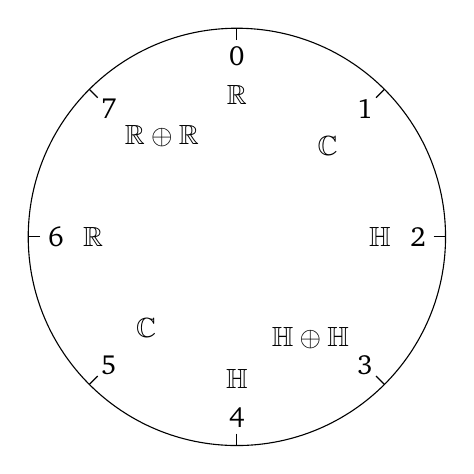
\begin{tikzpicture}
    \draw (0,0) circle[radius=2.65cm];
    \node[label=below:{$\mathbb{R}$}] at (90:2.3) {0};
    \node[label=below left:{$\mathbb{C}$}] at (45:2.3) {1};
    \node[label=left:{$\mathbb{H}$}] at (0:2.3) {2};
    \node[label={[label distance=-2mm]above left:{$\mathbb{H}\oplus\mathbb{H}$}}] at (-45:2.3) {3};
    \node[label=above:{$\mathbb{H}$}] at (-90:2.3) {4};
    \node[label=above right:{$\mathbb{C}$}] at (-135:2.3) {5};
    \node[label=right:{$\mathbb{R}$}] at (180:2.3) {6};
    \node[label={[label distance=-2mm]below right:{$\mathbb{R}\oplus\mathbb{R}$}}] at (135:2.3) {7};
    \foreach \a in {0,45,90,135,180,-135,-90,-45}
      \draw (\a:2.5) to (\a:2.65);
  \end{tikzpicture}
\] As I explained in \protect\hyperlink{week105}{``Week 105''}, this
clock easily lets you remember the real Clifford algebras in every
dimension and signature of spacetime. Bott periodicity explains why it
loops around after 8 hours. The spinorial chessboard presents the same
information in the form of an \(8\times 8\) grid. I won't draw it here,
but it's a picture of the Clifford algebras with \(p\) roots of \(-1\)
and \(q\) roots of \(1\) for \(p,q =0,1,2,3,4,5,6,7\). The black squares
correspond to cases that admit chiral spinors; the red ones correspond
to cases that don't. Black is when \(p+q\) is even; red is when it's
odd.

By the way, I have a little question: why does the above clock have a
reflection symmetry along the line joining \(\mathbb{R}+\mathbb{R}\) and
\(\mathbb{H}+\mathbb{H}\)?

Later, by coincidence, when I was in the library I discovered that
Chevalley's work on spinors has been reprinted:

\begin{enumerate}
\def\labelenumi{\arabic{enumi})}
\setcounter{enumi}{14}
\tightlist
\item
  Claude Chevalley, \emph{The Algebraic Theory of Spinors}, Springer,
  Berlin, 1991.
\end{enumerate}

It has a lot of neat stuff on ``pure spinors'', which are closely
related to the ``simple bivectors'' that describe 2-planes in
\(n\)-space. The latter play an important role in spin foam models of
quantum gravity, so I bet pure spinors will too.

Here's another fundamental text, which really helped get the whole
subject going:

\begin{enumerate}
\def\labelenumi{\arabic{enumi})}
\setcounter{enumi}{15}
\tightlist
\item
  Eli Cartan, \emph{The Theory of Spinors}, Dover Press, 1966.
\end{enumerate}

While I'm at it, I should mention this book by the infamous Pertti
Lounesto, which is also good:

\begin{enumerate}
\def\labelenumi{\arabic{enumi})}
\setcounter{enumi}{16}
\tightlist
\item
  Pertti Lounesto, \emph{Clifford Algebras and Spinors}, Cambridge U.
  Press, Cambridge, 1997.
\end{enumerate}

I also saw this book at a book fair:

\begin{enumerate}
\def\labelenumi{\arabic{enumi})}
\setcounter{enumi}{17}
\tightlist
\item
  Dominic Joyce, \emph{Compact Manifolds with Special Holonomy}, Oxford
  U. Press, Oxford, 2000.
\end{enumerate}

There's some incredible stuff here about \(7\)-dimensional Riemannian
manifolds whose holonomy groups lie in the exceptional Lie group
\(\mathrm{G}_2\). I bet this stuff is gonna be important in string
theory someday --- if it isn't already. After all, \(\mathrm{G}_2\) is
the automorphism group of the octonions, and it has a \(7\)-dimensional
irreducible representation on the imaginary octonions; as explained in
\protect\hyperlink{week104}{``Week 104''} by Robert Helling, the
octonions are secretly what let you write down the superstring
Lagrangian in 10d spacetime.

\begin{center}\rule{0.5\linewidth}{0.5pt}\end{center}

Footnote:

Andrzej Trautman answered my question about reflection symmetry in the
Clifford algebra clock by noting that
\[\mathrm{Cliff}(p,q) \otimes \mathbb{R}(2) = \mathrm{Cliff}(q+2,p)\]
where \(\mathbb{R}(2)\) is the algebra of \(2\times2\) real matrices. A
proof of this (actually well-known) fact appears in (7.8b) of his book.

In response to my list of most-cited papers, Aaron Bergman suggested the
following 261-page review article on the AdS-CFT correspondence:

\begin{enumerate}
\def\labelenumi{\arabic{enumi})}
\setcounter{enumi}{18}
\tightlist
\item
  O. Aharony, S. S. Gubser, J. Maldacena, H. Ooguri and Y. Oz, ``Large
  \(N\) field theories, string theory and gravity'', \emph{Phys. Rept.}
  \textbf{323} (2000) 183--386, preprint available as
  \href{https://arxiv.org/abs/hep-th/9905111}{\texttt{hep-th/9905111}}.
\end{enumerate}

For a similarly enormous review article on D-branes, try:

\begin{enumerate}
\def\labelenumi{\arabic{enumi})}
\setcounter{enumi}{19}
\tightlist
\item
  Clifford V. Johnson, ``D-brane primer'', preprint available as
  \href{https://arxiv.org/abs/hep-th/0007170}{\texttt{hep-th/0007170}}.
\end{enumerate}

Finally, it turns out that manifolds with \(\mathrm{G}_2\) holonomy
\emph{are} important in superstring theory, where they go by the name of
``Joyce manifolds''. Here are some places to read about them:

\begin{enumerate}
\def\labelenumi{\arabic{enumi})}
\setcounter{enumi}{20}
\item
  G. Papadopoulos and P. K. Townsend, ``Compactification of \(D=11\)
  supergravity on spaces of exceptional holonomy'', preprint available
  as
  \href{https://arxiv.org/abs/hep-th/9506150}{\texttt{hep-th/9506150}}.
\item
  B. S. Acharya, ``\(N=1\) heterotic-supergravity duality and Joyce
  manifolds'', preprint available as
  \href{https://arxiv.org/abs/hep-th/9508046}{\texttt{hep-th/9508046}}.

  ``\(N=1\) heterotic/M-theory duality and Joyce manifolds'', preprint
  available as
  \href{https://arxiv.org/abs/hep-th/9603033}{\texttt{hep-th/9603033}}.

  ``\(N=1\) M-theory-heterotic duality in three dimensions and Joyce
  manifolds'', preprint available as
  \href{https://arxiv.org/abs/hep-th/9604133}{\texttt{hep-th/9604133}}.

  ``Dirichlet Joyce manifolds, discrete torsion and duality'', preprint
  available as
  \href{https://arxiv.org/abs/hep-th/9611036}{\texttt{hep-th/9611036}}.

  ``M theory, Joyce orbifolds and super Yang-Mills'', preprint available
  as
  \href{https://arxiv.org/abs/hep-th/9812205}{\texttt{hep-th/9812205}}.
\item
  Chien-Hao Liu, ``On the global structure of some natural fibrations of
  Joyce manifolds'', preprint available as
  \href{https://arxiv.org/abs/hep-th/9809007}{\texttt{hep-th/9809007}}.
\end{enumerate}

I learned this thanks to Allen Knutson and Paul Schocklee. Paul also had
the following interesting comments:

\begin{quote}
John Baez wrote:
\end{quote}

\begin{quote}
\begin{quote}
There's some incredible stuff here about \(7\)-dimensional Riemannian
manifolds whose holonomy groups lie in the exceptional Lie group
\(\mathrm{G}_2\).\\
I bet this stuff is gonna be important in string theory someday --- if
it isn't already.
\end{quote}
\end{quote}

\begin{quote}
They are important!
\end{quote}

\begin{quote}
If you want to directly compactify \(11\)-dimensional
supergravity/M-theory to a theory with \(N=1\) supersymmetry in 4
dimensions, which is what people like for phenomenological reasons, you
need a \(7\)-dimensional manifold of \(\mathrm{G}_2\) holonomy (just as
you need manifolds of \(\mathrm{SU}(3)\) holonomy, i.e. Calabi-Yau
manifolds, in six dimensions). I have seen these referred to as ``Joyce
manifolds,'' after Dominic Joyce, who constructed several examples of
such spaces. (I didn't know there was so much known about them. I'll
have to check out the above book; I see that our library in Iceland has
a copy.)
\end{quote}

\begin{quote}
Unfortunately, these models are afflicted by the usual problem of 11-d
SUGRA compactifications, which is that they are non-chiral, so these
days people seem to be concentrating more on Horava-Witten
compactifications, with M-theory on \(S^1/\mathbb{Z}_2\) times a
Calabi-Yau, or on an orbifold.
\end{quote}

\begin{quote}
If you're interested, you might want to check out Papadopoulos and
Townsend, ``Compactification of D=11 supergravity on spaces of
exceptional holonomy,'' https://arxiv.org/abs/hep-th/9506150.
\end{quote}

\begin{quote}
-- Paul Shocklee Graduate Student, Department of Physics, Princeton
University Researcher, Science Institute, Dunhaga 3, 107 Reykjavk,
Iceland Phone: +354-525-4429
\end{quote}



\hypertarget{week155}{%
\section{August 16, 2000}\label{week155}}

It's a hot summer day here in Riverside, so I just want to have fun.
Break out the Klein bottles and Platonic solids!

I still remember the day as a kid when I first made a Möbius strip, and
saw how it didn't fall apart when cut in half. I could see it, but I
couldn't quite grok it. I was fascinated --- and more than a little
annoyed when it turned out my dad already knew about it.

I don't remember exactly when I first saw a Klein bottle, but I loved it
at first sight:

\begin{verbatim}
            A mathematician named Klein
            Thought the Möbius strip was divine.
            Said he: "If you glue 
            The edges of two
            You'll get a weird bottle like mine!"
\end{verbatim}

Recently, when I was trying to explain some stuff about Klein bottles to
my friend Oz on \texttt{sci.physics.research}, I bumped into the website
of a company that sells the things --- Acme Klein Bottles. I couldn't
resist mentioning to the world at large that I'd dearly like one. And lo
and behold, a regular reader of This Week's Finds took me up on this:
Timothy J. Kordas. After a few weeks, a handcrafted glass Klein bottle
arrived via United Parcel Service. It's great! --- it sits on my desk
now, gleaming contentedly. I think everybody should have one. You can
even buy them sliced in half, exhibiting the Möbius strip quite clearly:

\begin{enumerate}
\def\labelenumi{\arabic{enumi})}
\tightlist
\item
  Acme Klein bottles sliced in half,
  \texttt{http://www.kleinbottle.com/sliced\_klein\_bottles.htm}
\end{enumerate}

Meanwhile, I've been thinking about the Platonic solids lately, and also
their generalizations to higher dimensions --- the so-called ``regular
polytopes''. To really learn about regular polytopes, you have to go to
the source: the king of geometry, Harold Scott Macdonald Coxeter. But
for some reason I didn't get around to reading his books until just
recently:

\begin{enumerate}
\def\labelenumi{\arabic{enumi})}
\setcounter{enumi}{1}
\item
  H. S. M. Coxeter, \emph{Regular Polytopes}, 3rd edition, Dover, New
  York, 1973.

  \emph{Regular Complex Polytopes}, 2nd edition, Cambridge U. Press,
  Cambridge, 1991.
\end{enumerate}

Now my head is full of neat facts about regular polytopes, so I want to
rattle some off before I forget!

Let's start in 3 dimensions. I assume you're friends with the
tetrahedron, cube, octahedron, dodecahedron and icosahedron. But you
might not know all the nice relationships between them!

For example, there's a nice way to fit a tetrahedron snugly into a cube:
if you take every other vertex of the cube, you get the vertices of a
tetrahedron. And of course I mean a \emph{regular} tetrahedron --- I'm
not interested in any other kind, here. There are two ways to do this,
and if you put both these tetrahedra inside the cube, they combine to
form a star-shaped solid called the ``stella octangula''. This was
discovered and given its name by Kepler, who was really fond of this
sort of thing.

Here's a picture:

\begin{enumerate}
\def\labelenumi{\arabic{enumi})}
\setcounter{enumi}{2}
\tightlist
\item
  Eric Weisstein, stella octangula,
  \texttt{http://mathworld.wolfram.com/StellaOctangula.html}
\end{enumerate}

You can rotate it by grabbing it with your mouse!

Similarly, there is a nice way to fit a cube in a dodecahedron. The
dodecahedron has 20 vertices, and we can use 8 of these as the vertices
of a cube. This becomes obvious once we realize that these points are
the vertices of a dodecahedron: \[
  \begin{gathered}
    (\pm 1/G, \pm G, 0),
  \\(\pm G, 0, \pm 1/G),
  \\(0, \pm 1/G, \pm G)
  \\(\pm1, \pm1, \pm1).
  \end{gathered}
\] where \(G = (\sqrt{5} + 1)/2\) is the golden ratio and we get to pick
each of the plus or minus signs independently. The points
\((\pm1, \pm1, \pm1)\) form the vertices of a cube.

By rotating the whole picture, we get some other ways of putting a cube
in a dodecahedron: 5 in all. Any rotation of the dodecahedron permutes
these 5 cubes, and we get all even permutations of the cubes this way:
this is one nice way to prove that the rotational symmetry group of the
dodecahedron is \(A_5\) (the group of even permutations of 5 things).

If we put all 5 cubes inside the dodecahedron, we get a fancy shape that
would make a marvelous Christmas tree decoration --- I don't know what
it's called, but you can see a picture of it in Coxeter's ``Regular
Polytopes'', and also here:

\begin{enumerate}
\def\labelenumi{\arabic{enumi})}
\setcounter{enumi}{3}
\tightlist
\item
  Eric Weisstein, cube 5-compound,
  \texttt{http://mathworld.wolfram.com/Cube5-Compound.html}
\end{enumerate}

Now let's combine these two tricks. If we put a tetrahedron in a cube,
and then put the cube in a dodecahedron, we get a way of fitting the
tetrahedron snugly into the dodecahedron! If we choose one way of doing
this and then rotate the picture to get other ways, we get 5 tetrahedra
in the dodecahedron. Putting these all together gives a scary-looking
shape:

\begin{enumerate}
\def\labelenumi{\arabic{enumi})}
\setcounter{enumi}{4}
\tightlist
\item
  Eric Weisstein, tetrahedron 5-compound,
  \texttt{http://mathworld.wolfram.com/Tetrahedron5-Compound.html}
\end{enumerate}

but the coolest thing about this shape is that it has an inherent
handedness --- like a sugar molecule, it comes in ``levo'' and
``dextro'' forms! If we reflect it, we get 5 \emph{other} ways to put a
tetrahedron into a dodecahedron, for a total of 10. All of these
tetrahedra taken together form a mirror-symmetric shape:

\begin{enumerate}
\def\labelenumi{\arabic{enumi})}
\setcounter{enumi}{5}
\tightlist
\item
  Eric Weisstein, tetrahedron 10-compound,
  \texttt{http://mathworld.wolfram.com/Tetrahedron10-Compound.html}
\end{enumerate}

Okay. So far we've related the tetrahedron, the cube and the
dodecahedron. What about the other two Platonic solids: the octahedron
and icosahedron? Well, from the point of view of \emph{symmetry groups}
these guys are redundant. The octahedron is dual to the cube, so it has
the same rotational symmmetry group. Similarly, the icosahedron is dual
to the dodecahedron and has the same symmetry group.

From the group-theoretic viewpoint, here's what's really going on. Our
trick for fitting the tetrahedron in the cube lets us turn any symmetry
of the tetrahedron into a symmetry of the cube. The rotational symmetry
group of the tetrahedron is \(A_4\) --- that is, all even permutations
of the 4 vertices. The symmetry group of the cube is \(S_4\) --- that
is, all permutations of the 4 lines connecting opposite vertices. So
what we've got is a trick for making \(A_4\) into a subgroup of \(S_4\).

(This immediately leads to a little puzzle. There's an \emph{obvious}
way to find \(A_4\) as a subgroup of \(S_4\), since even permutations
are a special case of permutations. So: does the above trick give this
obvious way, or some other way?)

Anyway, it's also true that any way of fitting the tetrahedron in the
dodecahedron lets us turn any symmetry of the tetrahedron into a
symmetry of the dodecahedron. So we've also got a trick for making
\(A_4\) into a subgroup of \(A_5\).

(You might also think that our trick for fitting the cube in the
dodecahedron gives a way to turn any symmetry of the cube into a
symmetry of the dodecahedron. I thought this for a while, but it's not
true! For starters, if it \emph{were} true, we'd get a trick for making
\(S_4\) into a subgroup of \(A_5\) --- which is impossible, since the
order of the group \(S_4\) doesn't divide that of \(A_5\). And the
problem turns out to be this: a 90 degree rotation of the cube does not
correspond to a symmetry of the dodecahedron.)

Playing with this stuff would be a nice way to start learning group
theory --- but even if you already know group theory, it's sort of fun.
For more along these lines, try:

\begin{enumerate}
\def\labelenumi{\arabic{enumi})}
\setcounter{enumi}{6}
\tightlist
\item
  John Baez, Some thoughts on the number 6,
  \texttt{http://math.ucr.edu/home/baez/six.html}
\end{enumerate}

Check out the new link to Greg Egan's website illustrating some of the
concepts!

Now, despite their redundancy from the group-theoretic viewpoint, it's
unfair to leave the octahedron and icosahedron out in the cold. These
guys should be related somehow. After all, the octahedron has 12 edges,
while the icosahedron has 12 vertices. Is there any way we can exploit
this fact?

Yes! The octahedron is the only Platonic solid whose faces can be
colored black and white so that no two faces of the same color share an
edge. So go ahead: grab a regular octahedron and color it like that.
Next, pick an edge and start marching along it with the white face to
your left and the black face to your right. Go \(1/G\)th of the way,
where \(G\) is the golden ratio again, and mark this point with a dot.
Now do this for all the edges. You'll get 12 dots --- and these dots
form the vertices of a regular icosahedron!

Next, let's take a quick tour of the 4th dimension. This is the most
exciting dimension for regular polytopes. In all higher dimensions there
are only three --- analogues of the tetrahedron, cube and octahedron.
But in 4 dimensions, there are six.

I won't describe these systematically here. For that you should read
Coxeter's books, or if you're in a rush, my webpage:

\begin{enumerate}
\def\labelenumi{\arabic{enumi})}
\setcounter{enumi}{7}
\tightlist
\item
  John Baez, ``Platonic solids in all dimensions'',
  \texttt{http://math.ucr.edu/home/baez/platonic.html}
\end{enumerate}

Instead, I'll just talk about a cool relationship between my two
favorite 4d regular polytopes: the 24-cell and the 600-cell.

First let me set the stage, by reminding you what these look like. A
24-cell looks like this:

\begin{enumerate}
\def\labelenumi{\arabic{enumi})}
\setcounter{enumi}{8}
\tightlist
\item
  Eric Weisstein, 24-cell,
  \texttt{http://mathworld.wolfram.com/24-Cell.html}
\end{enumerate}

To visualize it on your own, first imagine a hypercube with vertices
\[(\pm1,\pm1,\pm1,\pm1)\] Then imagine the \(4\)-dimensional analogue of
an octahedron --- usually called a ``cross-polytope'' --- with vertices
\[
  \begin{gathered}
    (\pm2,0,0,0),
  \\(0,\pm2,0,0),
  \\(0,0,\pm2,0),
  \\(0,0,0,\pm2).
  \end{gathered}
\] The hypercube has 16 vertices and the cross-polytope has 8. I've set
things up so that all 24 of these points have the same distance from the
origin. These are the vertices of the 24-cell!

But the 24-cell does not get its name from having 24 vertices. It gets
its name from having 24 faces! It has 24 octahedral faces, 96 triangles,
96 edges and 24 vertices. The symmetry here comes from the fact that the
24-cell is self-dual --- which comes from the fact that we've built it
from two polytopes that are dual to each other: the hypercube and the
cross-polytope.

What would happen if we had tried this trick in 3 dimensions? Let's see!
Take a cube and take an octahedron. Center them both at the origin, line
them up nicely, and rescale them so all their vertices are the same
distance from the origin: say \[(\pm1,\pm1,\pm1)\] and \[
  \begin{gathered}
    (\pm\sqrt{3},0,0),
  \\(0,\pm\sqrt{3},0),
  \\(0,0,\pm\sqrt{3}).
  \end{gathered}
\] We get a shape with \(8 + 6 = 14\) vertices. But it's not a Platonic
solid --- it's a rhombic dodecahedron! Apparently this too was first
discovered by Kepler. You can view one, and even rotate it by hand, at
this webpage:

\begin{enumerate}
\def\labelenumi{\arabic{enumi})}
\setcounter{enumi}{9}
\tightlist
\item
  Kevin Brown, Kepler's rhombic dodecahedron,
  \texttt{http://www.seanet.com/\textasciitilde{}ksbrown/coinc2.htm}
\end{enumerate}

Here's another way to think about this stuff. Take two cubes, equal in
size. Chop one up into 6 pyramids, each having one face of the cube as
its base, and each having the cube's center as its apex. Now take these
6 pyramids and glue their bases onto the faces of the other cube. What
do you get? A rhombic dodecahedron! If can't visualize this, go here:

\begin{enumerate}
\def\labelenumi{\arabic{enumi})}
\setcounter{enumi}{10}
\tightlist
\item
  Mark Newbold's rhombic dodecahedron page,
  \texttt{http://dogfeathers.com/mark/rhdodec.html}
\end{enumerate}

Now do the same thing in 4 dimensions. Take two hypercubes, equal in
size. Chop one up into 8 ``hyperpyramids'', each having one face of the
hypercube as its base, and each having the hypercube's center as its
apex. Now take these hyperpyramids and glue their bases onto the faces
of the other hypercube. What do you get? The 24-cell!

(Of course, one can play this game in any dimension, but it works best
in dimension 4. I could explain why, but it's probably better to figure
it out yourself.)

Okay. Now for the 600-cell. This one is harder: it has 600 tetrahedral
faces, 1200 triangles, 720 edges, and 120 vertices. When Buckminster
Fuller died and went to heaven, he probably took up residence in one of
these. It looks like this:

\begin{enumerate}
\def\labelenumi{\arabic{enumi})}
\setcounter{enumi}{11}
\tightlist
\item
  Eric Weisstein, 600-cell,
  \texttt{http://mathworld.wolfram.com/600-Cell.html}
\end{enumerate}

Here's how you build one. Start with 600 regular tetrahedra. Take 20 of
them and glue them together so they all meet at one vertex and the
outside looks just like an icosahedron. Of course you can't do this in
flat \(3\)-dimensional space: there's ``wiggle room'' left over when you
try! So you have to bend the whole setup a little bit into the 4th
dimension, like a piece of a 4d geodesic dome. Then keep adding more
tetrahedra, always making sure that 20 meet at each vertex in an
icosahedral pattern. By the time you've used up all of them, your
600-cell will be complete --- a nice rigid structure.

Of course, if you're a mathematician, there are other more elegant ways
to build your 600-cell. For example: start with an icosahedron. Its
rotational symmetry group is a 60-element subgroup of
\(\mathrm{SO}(3)\). Using the double cover
\(\mathrm{SU}(2) \to \mathrm{SO}(3)\) lift this to a 120-element
subgroup of \(\mathrm{SU}(2)\). But \(\mathrm{SU}(2)\) is isomorphic to
the unit quaternions, so we get 120 points on the unit sphere in 4
dimensions. These are the vertices of the 600-cell!

In fact we can construct the 24-cell in the same way, as I explained in
\href{week91.html}{week91}. Here we start with the tetrahedron, whose
rotational symmetry group is a 12-element subgroup of
\(\mathrm{SO}(3)\), and we get 24 points on the unit sphere in 4
dimensions, which are the vertices of the 24-cell.

But if you really want to show off, you can build a 600-cell starting
from a 24-cell! Here's how. It's a bit like the trick where we started
with an octahedron, systematically marked a point \(1/G\)th of the way
along each edge, and got the vertices of an icosahedron. But it's
fancier.

Start with the 24-cell. Take any edge, start walking down it, and when
you've gone \(1/G\)th of the way, mark that point with a dot. Of course
these instructions are ambiguous, since I didn't tell you which end of
the edge to start at! I could tell you, but I won't --- I'll just say
that if you do it \emph{the right way}, you'll get 96 dots which are the
vertices of a marvelous polytope in 4 dimensions. It's not a regular
polytope, but it's ``semiregular'': it has 24 regular icosahedra and 120
regular tetrahedra as faces. Coxeter calls it \(s\{3,4,3\}\), but it
really deserves a more glamorous name.

Now as we've seen, in 4 dimensions there is a way to glue 20 tetrahedra
together in an icosahedral pattern. You can picture this as a squat
pyramid-shaped gadget with a regular icosahedron as base and 20
tetrahedral faces all meeting at the apex.

So: glue one of these pyramid-shaped gadgets onto each of the 24
icosahedral faces of our \(s\{3,4,3\}\). We get a polytope which has
\(20\times 24\) new tetrahedral faces in addition to the 120 original
tetrahedral faces of our \(s\{3,4,3\}\), for a total of 600. Voila ---
it's the 600-cell!

For the proof that all this works as advertised, read Coxeter's
``Regular Polytopes''. Note that it's really easier to work backwards:
start with the 600-cell, then truncate it to get \(s\{3,4,3\}\).

Okay, now for one last trick. I actually thought of this myself ---
though I can't believe it's new. It gives a way to see the vertices of
the 24-cell as a subset of the vertices of the 600-cell.

As I already said, the rotational symmetry group of the tetrahedron has
a ``double cover'' consisting of 24 unit quaternions, which happen to be
precisely the vertices of the 24-cell.

Similarly, the rotational symmetry group of the dodecahedron has a
``double cover'' consisting of 120 unit quaternions, which happen to be
precisely the vertices of the 600-cell.

Any way of fitting the tetrahedron snugly into the dodecahedron
therefore gives a way of making the vertices of the 24-cell into a
subset of the vertices of the 600-cell!

Now, we've already seen 10 ways of snugly fitting the tetrahedron into
the dodecahedron: 5 which make the ``levo'' form of that scary-looking
shape, and 5 which make the ``dextro'' form. The first 5 give 5
different ways of stuffing the 24-cell into the 600-cell. But the second
5 give nothing new.

So this trick actually gives us 5 ways of making the vertices of the
24-cell into a subset of the vertices of the 600-cell. And all these
ways have one vertex in common, corresponding to the element 1 of the
unit quaternions.

Okay, that's it for this week. No serious stuff this time. I just want
to mention that in addition to the above websites, there are a lot that
show polyhedra in a way that requires red-blue 3d glasses or a VRML
plugin. Since I don't have either of these, and you might not either,
I've avoided links to those pages. By the way, VRML stands for ``virtual
reality modelling language'', but it's really just a language for
delivering interactive 3d objects over the web. If you can handle VRML,
you can probably have a lot of fun here:

\begin{enumerate}
\def\labelenumi{\arabic{enumi})}
\setcounter{enumi}{12}
\tightlist
\item
  George W. Hart's Pavilion of Polyhedrality,
  \texttt{http://www.georgehart.com/pavilion.html}
\end{enumerate}

If you don't, you can still enjoy the annotated bibliography and links
to other websites. You can also get a lot out of Vladimir Bulatov's
collection of polyhedra without VRML, but again, it's better if you have
it:

\begin{enumerate}
\def\labelenumi{\arabic{enumi})}
\setcounter{enumi}{13}
\tightlist
\item
  Victor Bulatov's Polyhedra Collection,
  \texttt{http://www.physics.orst.edu/\textasciitilde{}bulatov/polyhedra/index.html}
\end{enumerate}

Finally, if you're good at crossing your eyes, you can see some
4-dimensional polytopes at this website, which also has a lot of cool
information on how the 4d regular polytopes are related to other
branches of math:

\begin{enumerate}
\def\labelenumi{\arabic{enumi})}
\setcounter{enumi}{14}
\tightlist
\item
  Tony Smith, 24-cell animation, 120-cell, 600-cell,
  \texttt{http://www.innerx.net/personal/tsmith/24anime.html}
\end{enumerate}

I thank Jim Heckman and Noam Elkies for helping me fix some errors in
the original version of this article.



\hypertarget{week156}{%
\section{September 17, 2000}\label{week156}}

This week I want to catch you up on some of the experiments that have
been going on lately. Mathematical physics is no fun without some
experiments to think about now and then. So here's some news about black
holes, superfluid hydrogen, T violation, the \(\tau\) neutrino, and the
Higgs boson.

I like black holes because they are a nice example of what general
relativity can do. Once upon a time they seemed very exotic, but now it
seems they're common. In particular, there appear to be black holes with
masses between a million and several billion times that of the Sun at
the centers of all galaxies with a ``bulge''. This includes galaxies
like the Milky Way, which has a central bulge in addition to a flat
spinning disk, and also elliptical galaxies, which consist solely of a
bulge. Many of these supermassive black holes emit lots of X-rays as
they swallow hapless stars. As I mentioned in
\href{week144.html}{week144}, the X-ray telescope Chandra has seen
evidence for about 70 million of these black holes!

Recently, two teams of researchers have found that the mass of these
central black holes is correlated very closely to the dispersion of
stellar velocities in the galaxy:

\begin{enumerate}
\def\labelenumi{\arabic{enumi})}
\item
  John Kormendy, ``Monsters at the heart of galaxy formation'',
  \emph{Science} \textbf{289} (2000), 1484--1485. Available online at
  \texttt{http://www.sciencemag.org/cgi/content/full/289/5484/1484}
\item
  Laura Ferrarese and David Merritt, ``A fundamental relation between
  supermassive black holes and their host galaxies'', \emph{Astrophys.
  J. Lett.} \textbf{539}, (2000) L9, preprint available as
  \href{https://arxiv.org/abs/astro-ph/0006053}{\texttt{astro-ph/0006053}}.
\item
  Karl Gebhardt et al, ``A relationship between nuclear black hole mass
  and galaxy velocity dispersion'', \emph{Astrophys. J. Lett.}
  \textbf{539}, (2000) L13, preprint available as
  \href{https://arxiv.org/abs/astro-ph/0006289}{\texttt{astro-ph/0006289}}.
\end{enumerate}

Tight correlations are a bit rare in astrophysics, so they tend to be
important when they exist. If you look at a graph you'll see how nice
this one is:

\begin{enumerate}
\def\labelenumi{\arabic{enumi})}
\setcounter{enumi}{3}
\tightlist
\item
  Supermassive Black Hole Group, ``Theory of black holes and galaxies'',
  \texttt{http://www.physics.rutgers.edu/\textasciitilde{}merritt/theory.htm}
\end{enumerate}

Ferrarese and Merrit estimate that the black hole mass grows as roughly
the 4.8th power of the stellar velocity dispersion, which they define as
the standard deviation of the radial component of the velocities of
stars in the galaxy.

But what does this correlation \emph{mean}? Astrophysicists are still
arguing about that. But at the very least, it suggests an intimate
relation between supermassive black holes and the process of galaxy
formation.

Part of the puzzle is that nobody knows how these supermassive black
holes formed. You see, until very recently, all we've ever seen are
small black holes formed by the collapse of a single star (between 3 and
20 solar masses), and these supermassive ones at the centers of
galaxies. But last year, people started seeing middle- sized ones!
Colbert and Mushotzky found black holes between 100 and 10,000 solar
masses in about half of 30 nearby spiral and elliptical galaxies that
they examined:

\begin{enumerate}
\def\labelenumi{\arabic{enumi})}
\setcounter{enumi}{4}
\item
  Ed Colbert's homepage,
  \texttt{http://www.pha.jhu.edu/\textasciitilde{}colbert/}

  E. J. M. Colbert and R. F. Mushotzky, ``The nature of accreting black
  holes in nearby galaxy nuclei'', preprint available as
  \href{https://arxiv.org/abs/astro-ph/9901023}{\texttt{astro-ph/9901023}}.
\end{enumerate}

Ptak and Griffiths found a black hole of over 460 solar masses in an
irregular galaxy called M82:

\begin{enumerate}
\def\labelenumi{\arabic{enumi})}
\setcounter{enumi}{5}
\tightlist
\item
  A. Ptak, R. Griffiths, ``Hard X-ray variability in M82: evidence for a
  nascent AGN?'', preprint available as
  \href{https://arxiv.org/abs/astro-ph/9903372}{\texttt{astro-ph/9903372}}.
\end{enumerate}

This is a ``starburst galaxy'', meaning that it's full of supernovae
going off like a big firework display. When a star dies in a supernova
explosion, that's when a neutron star or black hole is formed --- so it
seems likely that this black hole in M82 was formed by the merger of
several such black holes. Could we be seeing the gradual formation of a
supermassive black hole?

Maybe someday we'll understand the complete ecology of black holes. I
can't help but feel there's some important role they play which we don't
understand yet. (For one theory about this, see the end of
\href{week33.html}{week33}.)

Now: you've all heard how helium-4 becomes a superfluid below 2.18
kelvin and helium-3 does it below 2.4 millikelvin. But what about
superfluid hydrogen? Unlike helium, hydrogen is not a snobbish loner:
it's a friendly, sticky molecule. So usually it solidifies before it
gets cold enough to go superfluid! But in 1997, some folks at the
University of Illinois noticed a possible loophole: films of liquid
hydrogen about one molecule thick on a silver substrate should form a 2d
superfluid at a temperature of 1.2 kelvin. Here's a picture of a
computer simulation:

\begin{enumerate}
\def\labelenumi{\arabic{enumi})}
\setcounter{enumi}{6}
\tightlist
\item
  David Ceperley et al, ``Prospective superfluid molecular hydrogen'',
  \texttt{http://www.aip.org/physnews/graphics/html/h2.htm}
\end{enumerate}

Since then, other people have cooked up other schemes.

Now it seems people have actually made the stuff. Tiny amounts of it!
The way they do it is to take superfluid helium and put in a bit of
carbonyl sulfide (OCS) and hydrogen. About 14 to 16 hydrogen molecules
stick to the carbonyl sulfide molecule, and when the temperature drops
to .15 kelvin, these molecules form a superfluid. The hard part is
checking experimentally that this really happens --- and even
\emph{defining} what it means for a cluster of so few molecules to be a
superfluid. I can't explain the details; for that you'll have to read
the paper:

\begin{enumerate}
\def\labelenumi{\arabic{enumi})}
\setcounter{enumi}{7}
\tightlist
\item
  Slava Grebenev, Boris Sartakov, J. Peter Toennies, and Andrei F.
  Vilesov, ``Evidence for superfluidity in para-hydrogen clusters inside
  helium-4 droplets at 0.15 Kelvin'', \emph{Science} \textbf{5484}
  (2000), 1532--1535, available online at
  \texttt{http://www.sciencemag.org/cgi/content/abstract/289/5484/1532}
\end{enumerate}

Here ``para-hydrogen'' refers to a molecule of hydrogen where the spins
on the two nuclei are anti-parallel --- as opposed to
``ortho-hydrogen'', where they're lined up. The two states have
different properties and this matters a lot in delicate situations like
these.

Next: T violation. Once people thought the laws of physics were
symmetrical under exchanging either particles with their antiparticles,
left with right, or future with past. These three symmetries are called
C (for ``charge conjugation''), P (for ``parity'') and T (for ``time
reversal''). The weak interaction is now believed to violate all of
these.

Very briefly, the story goes like this: Yang and Lee won the Nobel prize
for helping discover P violation in the \(\beta\) decay of radioactive
cobalt back in 1956, though in retrospect it was only the sexism of the
Nobel committee that prevented Wu from sharing this prize --- she did
the actual experiment. In \(\beta\) decay, a neutron turns into a
proton, an electron and an electron anti-neutrino via the weak
interaction. Since the electron anti-neutrino only comes in a
right-handed form, this process violates P symmetry.

Cronin and Fitch won the Nobel prize for discovering in 1964 that
neutral kaons decay in a way that violates CP symmetry --- i.e., the
symmetry where you switch particles with their antiparticles \emph{and}
switch left with right. I believe that neutral kaons are still the only
system where CP violation has been seen.

Now there's something called the CPT theorem which says that various
reasonable axioms for a quantum field theory imply symmetry under the
\emph{combination} of C, P and T. For the math of this, the obvious
place to go is this classic text on axiomatic quantum field theory:

\begin{enumerate}
\def\labelenumi{\arabic{enumi})}
\setcounter{enumi}{8}
\tightlist
\item
  R. F. Streater and A. S. Wightman, \emph{PCT, Spin and Statistics, and
  All That}, Addison-Wesley, Reading, Massachusetts, 1989.
\end{enumerate}

In case you're worried, PCT is the same thing as CPT. I like this book a
lot. The only thing I dislike is how it unleashed a flood of physics
papers whose titles end with ``and all that''. For example:

\begin{itemize}
\tightlist
\item
  ``CFT, BCFT, ADE and all that''
\item
  ``Quantum cohomology and all that''
\item
  ``String theory, supersymmetry, unification, and all that''
\item
  ``Anti-de Sitter space, branes, singletons, superconformal field
  theories and all that''
\item
  ``The modified Bargmann-Wigner formalism: longitudinal fields, parity
  and all that''
\item
  ``The Zamolodchikov C-Function, classical closed string field theory,
  the Duistermaat-Heckman theorem, the renormalization group, and all
  that''
\end{itemize}

Enough! Listen, guys: it was funny once, but now it's just lame. Stop
it!

But I digress. Where was I? Oh yeah: given the CPT theorem, from CP
violation we can conclude T violation. The future and the past are
slightly different --- but of all the known forces, only the weak force
notices the difference! This is bizarre and fascinating. But the way we
reached this conclusion was not completely satisfying, since we needed
to assume the usual axioms of quantum field theory to get the CPT
theorem. What if the axioms are wrong? It would be better to have more
\emph{direct} evidence of T violation, given how important this issue
is.

So in the late 1990s, people in the CPLEAR collaboration at CERN did
some precision experiments on neutral kaon decay, and found more direct
evidence of T violation!

\begin{enumerate}
\def\labelenumi{\arabic{enumi})}
\setcounter{enumi}{9}
\item
  CPLEAR homepage,
  \texttt{http://cplear.web.cern.ch/cplear/Welcome.html}
\item
  CPLEAR collaboration, ``First direct observation of time-reversal
  non-invariance in the neutral kaon system'', \emph{Phys. Lett.}
  \textbf{B 444} (1998) 43, available online with all other papers by
  this collaboration at
  \texttt{http://cplear.web.cern.ch/cplear/cplear\_pub.html}
\end{enumerate}

Now we can all sit back and rack our brains even harder about what T
violation really \emph{means}. So far, all we know is that it arises
from the darkest corner of the Standard Model: the Kobayashi-Maskawa
matrix. This is a matrix describing quarks' couplings to the Higgs. The
fact that it's not diagonal means that the ``flavor eigenstates'' of the
quarks - up and down, strange and charmed, bottom and top --- are not
the ``mass eigenstates''. Why does the Kobayashi-Maskawa matrix equal
what it equals? Why is it of a form that violates T symmetry? Nobody
knows.

Another nice confirmation of what we already believed was the recent
discovery of direct evidence for the \(\tau\) neutrino. If you don't
remember the particles in the Standard Model, try
\href{week119.html}{week119}: you'll see that it has 3 generations of
quarks (listed above) and 3 generations of leptons: the electron, muon
and \(\tau\) and their corresponding neutrinos. Of the leptons, the
\(\tau\) is the heaviest and thus hardest to produce. Tau neutrinos are
produced by the decay of \(\tau\) particles, but since it's hard to make
these particles and hard to catch neutrinos, until recently nobody had
ever done the clinching experiment: creating a beam of a \(\tau\)
neutrinos and letting it collide with some stuff to form \(\tau\)
particles again.

On July 21st, 2000, the DONUT collaboration at Fermilab announced that
they had successfully done this experiment:

\begin{enumerate}
\def\labelenumi{\arabic{enumi})}
\setcounter{enumi}{11}
\tightlist
\item
  Christina Hebert, ``Phyisicists find first direct evidence for
  \(\tau\) neutrino at Fermilab'',
  \texttt{http://www.fnal.gov/directorate/public\_affairs/story\_neutrino/p1.html}
\end{enumerate}

In case you're wondering, ``DONUT'' stands for ``Direct Observation of
the Nu Tau'', where \(\nu_\tau\) is the standard abbrevation for
\(\tau\) neutrino.

In short, the final details of the Standard Model are all falling into
place just as expected --- except for the fact that neutrinos are doing
lots of weird stuff they shouldn't be doing! As I explained in
\href{week130.html}{week130}, neutrino physics is the big place for
surprises in particle physics these days. This is yet another reason why
it was good to directly observe the \(\tau\) neutrino.

And then, of course, there's the Higgs --- the final particle in the
Standard Model. As you've probably heard, we're getting awfully close to
seeing it --- or at least definitively \emph{not} seeing it. Right now
they're looking for it at LEP --- the big particle accelerator at CERN,
in Geneva. They're just about to shut LEP down, since it's done pretty
much all it can do, and they need to deactivate it to build an even more
powerful accelerator --- LHC, the Large Hadron Collider. But at the last
minute they decided to extend its life to November 2nd, 2000:

\begin{enumerate}
\def\labelenumi{\arabic{enumi})}
\setcounter{enumi}{12}
\tightlist
\item
  LEP shutdown postponed by one month,
  \texttt{http://press.web.cern.ch/Press/Releases00/PR08.00ELEPRundelay.html}
\end{enumerate}

They're going for broke, boosting its power to the utter max, so that
they can see hints of the Higgs as long as its mass is 114 GeV or so. In
fact they have already seen a couple of events that suggest a Higgs of
about this mass.

Whether or not LEP sees the Higgs the folks at the Tevatron at Fermilab
should see it when they start Run II in a while, as long as its mass
below 130 GeV. And if \emph{they} don't see it, folks at CERN should see
it with the LHC accelerator by around 2005, as long as its mass is below
180 GeV. A Higgs more massive than that would mean the Standard Model is
seriously screwed up, so at that point, even \emph{not} seeing the Higgs
would be an important discovery.

The folks getting ready to analyze the Run II data at the Tevatron are
doing so with a few theories in mind: the Standard Model, the minimal
supersymmetric extension of the Standard Model, and a
``next-to-minimal'' supersymmetric extension. This is a major project;
you can find lots of details here:

\begin{enumerate}
\def\labelenumi{\arabic{enumi})}
\setcounter{enumi}{13}
\tightlist
\item
  Higgs Working Group webpage,
  \texttt{http://fnth37.fnal.gov/higgs/higgs.html}
\end{enumerate}

That's basically it for this week. I just have a couple of questions
about CPT. A while back on sci.physics.research I emphasized a little
theorem that says: any self-dual irreducible unitary group
representation H must admit an antiunitary intertwiner
\(J\colon H \to H\) with either \(J^2 = 1\) or \(J^2 = -1\). In the
first case \(H\) comes from a real representation; in the second case it
comes from a quaternionic representation. For more details, try this:

\begin{enumerate}
\def\labelenumi{\arabic{enumi})}
\setcounter{enumi}{14}
\tightlist
\item
  John Baez, Symplectic, quaternionic, fermionic,
  \texttt{http://math.ucr.edu/home/baez/symplectic.html}
\end{enumerate}

Now, after I mentioned this, someone who goes by the name of ``squark''
suggested that the CPT operator for massive spin-\(1/2\) particles was
an antiunitary intertwiner with \((\mathrm{CPT})^2 = -1\). I'm not sure
this is true, but it's definitely antiunitary, so we have an intesting
question: which unitary irreducible representations of the Poincare
group are self-dual? Of these, which come from real representations and
which come from quaternionic ones? My hunch is that the bosonic (i.e.
integral-spin) reps are real and the fermionic (i.e.~half-integral-spin)
reps are quaternionic. And then the question is: is the operator \(J\)
just the the CPT operator? This would certainly shed some nice
mathematical light on the meaning of CPT symmetry.

By the way, This Week's Finds has a nice new feature, courtesy of
Laurent Bartholdi: now you can search all the old issues for a keyword
or phrase! This is very useful, at least for me. Check it out on my
website.

\begin{center}\rule{0.5\linewidth}{0.5pt}\end{center}

Footnotes:

Squark found in Volume 1 of Weinberg's ``Quantum Field Theory'' that the
CPT operator on the Hilbert space of a spin-\(j\) representation of the
Poincare group is an antiunitary operator with
\((\mathrm{CPT})^2 = -1^{2j}\). So indeed we do have
\((\mathrm{CPT})^2 = 1\) in the bosonic case, making these
representations real, and \((\mathrm{CPT})^2 = -1\) in the fermionic
case, making these representations quaternionic.

Allen Knutson points out that Streater and Wightman's title ``PCT, Spin
and Statistics, and All That'' was itself modelled after that of Sellar
and Yeatman's humorous history: ``1066 and all that; a memorable history
of England, comprising all the parts you can remember including one
hundred and three good things, five bad kings and two genuine dates.''

Martin Hardcastle wonders if Streater and Wightman were inspired by the
similarity of their names to those of Sellar and Yeatman!



\hypertarget{week157}{%
\section{September 24, 2000}\label{week157}}

I never write issues of This Week's Finds about topics that people
request. I only write about what I happen to be studying at a given
moment --- nothing else seems to work. But when my friend Minhyong Kim
asked me to do an issue on Young diagrams, I decided to break this rule
just once. Young diagrams are too cool to ignore.

Physics relies a lot on \emph{symmetry} to simplify problems, and there
are two kinds of diagrams that show up a lot in this context: Dynkin
diagrams and Young diagrams.

Dynkin diagrams first show up when you study shapes with lots of
reflection symmetries, like crystals and Platonic solids. They wind up
being good for all sorts of other stuff, like classifying simple Lie
groups and their representations. I talked about them in
\protect\hyperlink{week62}{``Week 62''} --
\protect\hyperlink{week65}{``Week 65''}.

But what about Young diagrams? These are also important for studying
group representations, but for a more limited class of groups: the
``classical'' groups.

As with composers of music, there's no precise list of groups that count
as ``classical''. But in general, a classical group should consist of
linear transformations that preserve some nice geometrical structure on
a vector space. A good example is \(\mathrm{SU}(N)\), the group of all
linear transformations of an \(N\)-dimensional complex vector space that
preserve an inner product and volume form. In less elevated language,
\(\mathrm{SU}(N)\) is the group of all \(N\times N\) unitary matrices
with determinant \(1\).

The symmetric group \(S_n\) may also be considered an honorary classical
group, even though it's defined in terms of a \emph{set} rather than a
\emph{vector space}. \(S_n\) is the group of all permutations of an
\(n\)-element set.

Rather amazingly, Young diagrams can be used to classify all 3 of these
things, which at first seem quite different in flavor:

\begin{itemize}
\tightlist
\item
  conjugacy classes in \(S_n\)
\item
  irreducible representations of \(S_n\)
\item
  irreducible representations of \(\mathrm{SU}(N)\)
\end{itemize}

Let me sketch how this goes, and then say a bit about the \emph{other}
things you can do with Young diagrams.

Say we have any permutation \(g\) in \(S_n\), like this: \[
  \begin{aligned}
    1 &\to 2
  \\2 &\to 4 
  \\3 &\to 3
  \\4 &\to 1
  \\5 &\to 6
  \\6 &\to 5
  \\7 &\to 7  
  \end{aligned}
\] Note that 1 gets mapped to 2, which gets mapped to 4, which gets
mapped back to 1 again. Similarly, 5 gets mapped to 6, which gets mapped
back to 5. The number 3 gets mapped to itself right away, as does 7. No
matter where we start, we always cycle back eventually. So our
permutation consists of a bunch of ``cycles'': \[(1,2,4) (5,6) (3) (7)\]
and writing down this ``cycle decomposition'' completely describes the
permutation. To simplify life, we always write down these cycles in
order of decreasing length. We also write the lowest number in each
cycle first.

Now suppose we conjugate our permutation \(g\) by some other
permutation, say \(h\). This gives the permutation \(hgh^{-1}\). How
does the cycle decomposition of this compare with that of \(g\)? It
looks almost the same! For example, it might look like this:
\[(2,7,6) (1,3) (4) (5)\] There are the same number of cycles, each the
same length as before. The only thing that changes are the numbers in
each cycle. These get switched around by means of the permutation \(h\).

In short, when we conjugate a permutation, all that remains unchanged is
the picture we get by writing down its cycle decomposition and blotting
out the specific numbers in each cycle, like this:
\[(\square,\square,\square) (\square,\square) (\square) (\square)\]
Folks usually write each cycle as a row, like this: \[
  \begin{array}{lll}
    \square&\square&\square
  \\\square&\square&
  \\\square&&
  \\\square&&
  \end{array}
\] This is called a ``Young diagram''! So a Young diagram is just a
bunch of rows of boxes, arranged in order of decreasing length.

Okay: so far I've shown how conjugacy classes of permutations in \(S_n\)
correspond to Young diagrams with a total of \(n\) boxes. Now I want to
do the same for irreducible representations of \(S_n\).

This is cool for the following reason: for any finite group, the number
of irreducible representations is the same as the number of conjugacy
classes of group elements. But in general there's no natural way to
match up irreducible representations with conjugacy classes. The group
\(S_n\) just happens to be specially nice in this way.

Here I must turn up the math level slightly\ldots{} for example, I'll
assume you know what ``irreducible representations'' means! I'll even
show off by calling them ``irreps'' for short. But to be nice, I'll
start by reviewing some general facts about representations of finite
groups.

Suppose \(G\) is a finite group. Then \(G\) has only finitely many
irreps, all finite-dimensional. Every finite-dimensional representation
of G is a direct sum of copies of these irreps.

To get our hands on these irreps, let \(\mathbb{C}[G]\) be the space of
formal linear combinations of elements of \(G\). This is called the
``group algebra'' of \(G\), since it becomes an algebra using the
product in \(G\). Any representation of the group \(G\) becomes a
representation of \(\mathbb{C}[G]\) in an obvious way, and vice versa.

With some work, one can show that \(\mathbb{C}[G]\) is isomorphic to an
algebra of block diagonal matrices. For example, \(\mathbb{C}[S_3]\) is
isomorphic to the algebra of matrices like this: \[
  \left(
    \begin{array}{cccc}
      * & * & 0 & 0
    \\* & * & 0 & 0
    \\0 & 0 & * & 0
    \\0 & 0 & 0 & *
    \end{array}
  \right)
\] where the \(*\) entries can be any complex number whatsoever. Since
matrices act on vectors by matrix multiplication, we can use this to get
a bunch of representations of \(\mathbb{C}[G]\), and thus of \(G\) ---
one representation for each block. And this trick gives us all the
irreps of \(G\)! For example, \(S_3\) has one \(2\)-dimensional irrep,
coming from the \(2\times 2\) block in the above matrix, and two
\(1\)-dimensional irreps, coming from the two \(1\times 1\) blocks.

This wonderful fact does not solve all our problems. If someone hands us
a finite group \(G\), we still need to work to find which algebra of
block diagonal matrices \(\mathbb{C}[G]\) is isomorphic to. How do we do
this?

The trick is to find elements of \(\mathbb{C}[G]\) corresponding to
matrices that are the identity matrix in one block and zero in the rest,
like these: \[
  \underbrace{
    \left(
      \begin{array}{cccc}
        1&0&0&0
      \\0&1&0&0
      \\0&0&0&0
      \\0&0&0&0
      \end{array}
    \right)}_{p_1}
  \qquad
  \underbrace{
    \left(
      \begin{array}{cccc}
        0&0&0&0
      \\0&0&0&0
      \\0&0&1&0
      \\0&0&0&0
      \end{array}
    \right)}_{p_2}
  \qquad
  \underbrace{
    \left(
      \begin{array}{cccc}
        0&0&0&0
      \\0&0&0&0
      \\0&0&0&0
      \\0&0&0&1
      \end{array}
    \right)}_{p_3}
\] If we can find these guys, the rest is easy: \(\mathbb{C}[G]\) is a
direct sum of ``blocks'' \[\{p_i a p_i \mid a \in\mathbb{C}[G]\}\] each
of which is isomorphic to some algebra of \(n\times n\) matrices.

How do we find these guys \(p_i\) in \(\mathbb{C}[G]\)? It's actually
pretty straightforward to characterize them:

\begin{itemize}
\tightlist
\item
  They are idempotent: \(p_i^2 = p_i\).
\item
  They are central: \(p_i x = x p_i\) for all \(x\) in
  \(\mathbb{C}[G]\).
\item
  They are minimal: if \(p_i\) is the sum of two central idempotents,
  one of them must be zero.
\end{itemize}

So we've reduced the problem of finding the irreps of a finite group
\(G\) to the problem of finding ``minimal central idempotents'' in the
group algebra \(\mathbb{C}[G]\).

To go further, we need to know more about our group \(G\). So now I'll
take \(G\) to be the permutation group \(S_n\) and tell you how to get
the minimal central idempotents. We'll get one for each Young diagram
with \(n\) boxes!

Say we have a Young diagram with \(n\) boxes, like this: \[
  \begin{array}{lll}
    \square&\square&\square
  \\\square&\square&
  \\\square&&
  \\\square&&
  \end{array}
\] Then we can pack it with numbers from \(1\) to \(n\) like this: \[
  \begin{array}{lll}
    1&2&3
  \\4&5&
  \\6&&
  \\7&&
  \end{array}
\] There are a bunch of permutations in \(S_n\) called ``column
permutations'', that only permute the numbers within each column of our
Young diagram. And there are a bunch called ``row permutations'', that
only permute the numbers within each row.

We can form an idempotent \(p\) in \(\mathbb{C}[S_n]\) that
antisymmetrizes over all column permutations. We get \(p\) by taking the
sum of all \emph{even} column permutations minus the sum of all
\emph{odd} column permutations, and then dividing by the total number of
column permutations.

Similarly, we can form an idempotent \(q\) in \(\mathbb{C}[S_n]\) that
symmetrizes over all row permutations. We get \(q\) by taking the sum of
all row permutations divided by the number of row permutations.

Now here's the cool part: \(pq\) is a minimal central idempotent in
\(\mathbb{C}[S_n]\), and we get all minimal central idempotents this
way! This isn't very obvious, but I went over the proof before writing
this, so I know it's true.

Consider \(n = 3\), for example. There are 3 Young diagrams in this
case: \[
  \begin{array}{lll}
    \square&\square&\square
  \end{array}
  \qquad\quad
  \begin{array}{lll}
    \square&\square&
  \\\square
  \end{array}
  \qquad\quad
  \begin{array}{lll}
    \square
  \\\square
  \\\square
  \end{array}
\] so \(S_3\) has 3 minimal central idempotents and thus 3 irreps,
confirming something I already said.

There is a lot more to say about this, but now I want to switch gears
and tell you how representations of \(\mathrm{SU}(N)\) are classified by
Young diagrams. Since \(\mathrm{SU}(N)\) consists of \(N\times N\)
matrices, it has an obvious representation on the vector space
\(\mathbb{C}^N\), which people call the ``fundamental'' representation.
This is an irrep. If we're trying to cook up irreps of
\(\mathrm{SU}(N)\), this is an obvious place to start.

How can we get a bunch of representations of \(\mathrm{SU}(N)\) starting
from the fundamental representation? One way is to take the fundamental
representation and tensor it with itself a bunch of times, say \(n\)
times:
\[\underbrace{\mathbb{C}^N\otimes\mathbb{C}^N\otimes\ldots\otimes\mathbb{C}^N}_{\mbox{$n$ copies}}\]
There's no reason in the world this new representation should be
irreducible. But we can try to chop it up into irreducible bits. And the
easiest way to do this is to look for bits that transform in nice ways
when we permute the \(n\) copies of \(\mathbb{C}^N\). In physics lingo,
we have a space of tensors with \(n\) indices, and we can look for
subspaces consisting of tensors that transform in specified ways when we
permute the indices. For example, there will be a subspace consisting of
``totally symmetric'' tensors that don't change at all when we permute
the indices. And a subspace of ``totally antisymmetric'' tensors that
change sign whenever we interchange two indices. And so on\ldots.

But to make the ``and so on'' precise, we need Young diagrams. After
all, these describe all the representations of the permutation group.

Here's how it works. The space
\[V = \underbrace{\mathbb{C}^N\otimes\mathbb{C}^N\otimes\ldots\otimes\mathbb{C}^N}_{\mbox{$n$ copies}}\]
is not only a representation of \(\mathrm{SU}(N)\); it's also a
representation of \(S_n\). And the actions of these two groups commute!
This means that we can chop up \(V\) into subspaces using the minimal
central idempotents in \(S_n\), and each of these subspaces will be a
representation of \(\mathrm{SU}(N)\).

This much is obvious. The really cool part is that all these subspaces
are \emph{irreducible} representations of \(\mathrm{SU}(N)\). Even
better, we get \emph{all} the irreps of \(\mathrm{SU}(N)\) by this
process, as we let \(n\) vary.

In other words, any Young diagram gives us an irrep of
\(\mathrm{SU}(N)\) consisting of tensors that transform in a certain way
under permutation of indices, and we get all irreps this way.

If you think about it, some of these irreps will be a bit silly. If we
have a Young diagram with more than \(N\) rows, we'll be
antisymmetrizing over more than \(N\) indices, which gives a
zero-dimensional representation of \(\mathrm{SU}(N)\). We can ignore
these.

Also, if we have a Young diagram that has just one column and exactly
\(N\) rows, we'll get the space of completely antisymmetric tensors with
\(N\) indices. This is a \(1\)-dimensional space. Applying a matrix in
\(\mathrm{SU}(N)\) to a tensor of this sort just multiplies it by the
determinant of that matrix, which is 1 by the definition of
\(\mathrm{SU}(N)\). So this Young diagram gives the trivial
representation of \(\mathrm{SU}(N)\). That's not too silly --- the
trivial representation is important, in its own trivial sort of way. But
notice: the trivial representation is already described by the Young
diagram with \emph{no} boxes! So it's redundant to also consider the
Young diagram with one column and \(N\) rows.

By the same logic, we can remove any column with exactly \(N\) rows from
a Young diagram without changing the rep of \(\mathrm{SU}(N)\) that we
get.

So here's the bottom line: irreps of \(\mathrm{SU}(N)\) correspond in a
1-1 way with Young diagrams having fewer than \(N\) rows.

Okay, I've shown you how Young diagrams classify conjugacy classes of
\(S_n\), irreps of \(S_n\), and irreps of \(\mathrm{SU}(N)\). But this
is really just the tip of the iceberg!

First of all, we can use Young diagrams packed with numbers, called
``Young tableaux'', to do all sorts of calculations involving irreps of
\(S_n\) and \(\mathrm{SU}(N)\). Say we tensor two irreps and want to
decompose it as a direct sum of irreps: how do we do it? Well, we play a
little game with Young tableaux and out pops the answer. One relevant
buzzword is ``Littlewood-Richardson rules''. Or say we have an irrep of
\(S_n\) and want to know how it decomposes into irreps when we restrict
it to a subgroup like \(S_{n-1}\). Or the same for \(\mathrm{SU}(N)\)
and \(\mathrm{SU}(N-1)\). How do we do this? More messing with Young
tableaux. Here one relevant buzzword is ``branching rules''.

I'll warn you right now: there is an \emph{enormous} literature on this
stuff. The combinatorics of Young diagrams is one of those things that
everyone has worked on, from hardnosed chemists to starry-eyed category
theorists. It takes a lifetime to master this material, and I certainly
have \emph{not}. But learning even a little is fun, so don't be
\emph{too} scared.

Second of all, Young diagrams are also good for studying the
representations of other classical groups, notably \(\mathrm{GL}(N)\),
\(\mathrm{SL}(N)\), \(\mathrm{O}(N)\), \(\mathrm{SO}(N)\),
\(\mathrm{U}(N)\) and \(\mathrm{Sp}(N)\). All these groups have an
obvious ``fundamental representation'', and we can cook up lots of reps
by taking the nth tensor power of the fundamental representation and
hitting it with minimal central idempotents in \(\mathbb{C}[S_n]\). The
story I just told you for \(\mathrm{SU}(N)\) can be repeated with slight
or not-so-slight variations for all these other groups.

Third, we can ``\(q\)-deform'' the whole story, replacing any one of
these classical groups by the associated ``quantum group'', and
replacing \(\mathbb{C}[S_n]\) by the corresponding ``Hecke algebra''.
This is really important in topological quantum field theory and the
theory of type II subfactors.

Fourth, there are nice relationships between Young diagrams and
algebraic geometry, like the ``Schubert calculus'' for the cohomology
ring of a Grassmanian.

And there's a lot more, but I have to stop somewhere.

So, how does one start learning this stuff?

If you have a certain amount of patience for old-fashioned terminology,
I might recommend going back to the classic text on classical groups:

\begin{enumerate}
\def\labelenumi{\arabic{enumi})}
\tightlist
\item
  Hermann Weyl, \emph{The Classical Groups, Their Invariants and
  Representations}, Princeton U. Press, Princeton, 1997.
\end{enumerate}

Weyl coined the term ``classical groups'' for the purposes of this book,
which was first published in 1939. His prose is beautiful, but I warn
you, this book is not the way to learn Young diagrams in a hurry.

For a user-friendly approach that's aimed at physicists, but still
includes proofs of all the key results, you can't beat this:

\begin{enumerate}
\def\labelenumi{\arabic{enumi})}
\setcounter{enumi}{1}
\tightlist
\item
  Irene Verona Schensted, \emph{A Course on the Applications of Group
  Theory to Quantum Mechanics}, NEO Press, Box 32, Peaks Island, Maine.
\end{enumerate}

A girlfriend of mine gave me a copy when I was a college student, but
only much later did I realize how great a book it is. Unfortunately it's
out of print! Someone should reprint this gem.

Here's another book that covers Young diagrams together with
applications to physics:

\begin{enumerate}
\def\labelenumi{\arabic{enumi})}
\setcounter{enumi}{2}
\tightlist
\item
  Shlomo Sternberg, \emph{Group Theory and Physics}, Cambridge U. Press,
  Cambridge, 1994.
\end{enumerate}

Both these books, but especially the latter, describe applications of
Young diagrams to particle physics, like Gell-Mann's famous ``eight-fold
way'', which was based on positing an \(\mathrm{SU}(3)\) symmetry
between the up, down and strange quarks.

Then there are more advanced texts, for when your addiction to Young
diagrams becomes more serious. For the combinatorial side of things,
these are good:

\begin{enumerate}
\def\labelenumi{\arabic{enumi})}
\setcounter{enumi}{3}
\item
  Gordon Douglas James and Adalbert Kerber, \emph{The Representation
  Theory of the Symmetric Group}, Addison-Wesley, Reading,
  Massachusetts, 1981.
\item
  Bruce Eli Sagan, \emph{The Symmetric Group: Representations,
  Combinatorial Algorithms, and Symmetric Functions}, Wadsworth and
  Brooks, Pacific Grove, California, 1191.
\end{enumerate}

For a more conceptual approach to representation theory that puts Young
diagrams in a bigger context, try this:

\begin{enumerate}
\def\labelenumi{\arabic{enumi})}
\setcounter{enumi}{5}
\tightlist
\item
  Roe Goodman and Nolan R. Wallach, \emph{Representations and Invariants
  of the Classical Groups}, Cambridge University Press, Cambridge, 1998.
\end{enumerate}

It's sort of an updated version of Weyl's book. Finally, here's a
mathematically sophisticated book that really gives you a Young diagram
workout:

\begin{enumerate}
\def\labelenumi{\arabic{enumi})}
\setcounter{enumi}{6}
\tightlist
\item
  William Fulton, \emph{Young Tableaux: With Applications to
  Representation Theory and Geometry}, Cambridge U. Press, Cambridge,
  1997.
\end{enumerate}

Now, my friend Allen Knutson is a real Young diagram fiend. Together
with Terry Tao, he helped prove something called ``Horn's conjecture'',
which had been bugging people for decades, and has implications for a
huge number of questions. I have a feeling Allen is going to send me a
nasty email saying that I didn't actually say anything
\emph{interesting} about Young diagrams. In an attempt to pacify him,
I'll direct you to Fulton's excellent review article on this subject:

\begin{enumerate}
\def\labelenumi{\arabic{enumi})}
\setcounter{enumi}{7}
\tightlist
\item
  William Fulton, ``Eigenvalues, invariant factors, highest weights, and
  Schubert calculus'', \emph{Bull. Amer. Math. Soc.} \textbf{37} (2000),
  209--249, also available as
  \href{http://arXiv.org/abs/math.AG/9908012}{\texttt{math.AG/9908012}}.
\end{enumerate}

as well as Allen and Terry's papers on the subject:

\begin{enumerate}
\def\labelenumi{\arabic{enumi})}
\setcounter{enumi}{8}
\item
  Allen Knutson and Terence Tao, ``The honeycomb model of
  \(\mathrm{GL}(n)\) tensor products I: the saturation conjecture'',
  preprint available as
  \href{http://arXiv.org/abs/math.RT/9807160}{\texttt{math.RT/9807160}}
\item
  Allen Knutson, ``The symplectic and algebraic geometry of Horn's
  problem'', preprint available as
  \href{http://arXiv.org/abs/math.LA/9911088}{\texttt{math.LA/9911088}}.
\item
  Allen Knutson and Terence Tao, ``Honeycombs and sums of Hermitian
  matrices'', preprint available as
  \href{http://arXiv.org/abs/math.RT/0009048}{\texttt{math.RT/0009048}}
\end{enumerate}

But I should also mention the question that Horn's conjecture settles!

There are many ways to phrase it; here's the easiest one. If you know
the eigenvalues of two \(n\times n\) Hermitian matrices \(A\) and \(B\),
what are the possible eigenvalues of their sum? There are a bunch of
linear inequalities that must hold; find a necessary and sufficient set.

This may not seem related to Young diagrams, but it is\ldots.

\begin{center}\rule{0.5\linewidth}{0.5pt}\end{center}

\begin{quote}
\emph{Devin had been studying this region for ten years, poking his way
through a place not much larger than the town in which he lived, and had
still not deciphered half its routes. This hugeness inside of smallness
creates a matrix of intersections, precious and incalculable channels
one after the next. It is a fractal landscape like the surface of a
leaf, veins within veins, or the arborescent feathers of ice forming
barbs within barbs across the surface of a pond.}

--- Craig Childs, Soul of Nowhere
\end{quote}



\hypertarget{week158}{%
\section{October 16, 2000}\label{week158}}

Like lots of mathematicians these days, I'm trying to understand
M-theory. It's a bit difficult, partially because the theory doesn't
really \emph{exist} yet. If it existed, it would explain lots of stuff:
on that everyone agrees. But nobody knows how to formulate M-theory in a
precise way, so you can't open up a paper and stare at ``the fundamental
equation of M-theory'', or anything like that. There are some
conjectures about what M-theory might be like, but no solid agreement.

One thing that \emph{does} exist is \(11\)-dimensional supergravity.
This is supposed to be some kind of classical limit of M-theory. But the
good thing is, it's a classical field theory with a Lagrangian that you
can write down and ponder to your heart's content. So I'm trying to
learn a bit about this.

Unfortunately, being a mathematician, I like to understand everything
rather carefully, preferably in a conceptual way that doesn't involve
big equations with indices dangling all over the place. This is slowing
me down, because all the descriptions I've seen make \(11\)-dimensional
supergravity look sort of ugly, when in fact it should be really pretty.
The physicists always point out that it's a lot simpler than the
supergravity theories in lower dimensions. On that I agree! But I don't
find it to be quite as simple as I'd like.

Now, mathematicians always whine like this when they are trying to learn
physics that hasn't been pre-processed by some other mathematician. So
just to show that I'm not completely making this stuff up, let me show
you the Lagrangian for 11d supergravity, as taken from the famous string
theory text by Green, Schwarz and Witten (see
\protect\hyperlink{week118}{``Week 118''}): \[
  \begin{aligned}
    L =
    &- \left(\frac{1}{2k^2}\right) eR
  \\&- \left(\frac{1}{2}\right) e\psi_M^* \Gamma^{MNP} D_N\left[\frac{\omega+\omega'}{2}\right]\psi_P
  \\&- \left(\frac{1}{48}\right) eF^2
  \\&- \left(\frac{\sqrt{2}k}{384}\right) e(\psi_M^* \Gamma^{MNPQRS}\psi_S + 12\psi^{*N}\Gamma^{PQ}\psi^R)(F+F')_{NPQR}
  \\&- \left(\frac{\sqrt{2}k}{3456}\right) \varepsilon^{M_1\ldots M_{11}}F_{M_1\ldots M_4}F_{M_5\ldots M_8}A_{M_9\ldots M_{11}}
  \end{aligned}
\] For comparison, here's the Lagrangian for ordinary gravity:
\[L = e R\] Here \(e\) is the volume form and \(R\) is the Ricci scalar
curvature. Of course, there is a lot of stuff packed into this
``\(R\)''. General relativity didn't look so slick when Einstein first
made it up! But by now, mathematicians have gnawed away at it for long
enough that there's a nice theory of differential geometry, where after
a few months of work you learn about ``\(R\)''. And after you've done
this work, you realize that ``\(R\)'' is a very natural concept. I want
to get to this point for the Lagrangian for 11d supergravity, but I'm
not there yet.

You'll note that apart from a constant, the Lagrangian for 11d
supergravity starts out basically like the Lagrangian for ordinary
gravity. So \emph{that} part I understand. It's just the other stuff
that's the problem.

Modulo some subtleties discussed below, the whole Lagrangian is built
from just three ingredients, which are the three basic fields in the
theory:

\begin{enumerate}
\def\labelenumi{\Alph{enumi})}
\item
  a Lorentzian metric \(g\) on the \(11\)-dimensional manifold
  representing spacetime,
\item
  a field \(\psi\) on this manifold which takes values in the real
  spin-\(3/2\) representation of \(\mathrm{SO}(10,1)\),
\item
  a \(3\)-form field \(A\) on this manifold.
\end{enumerate}

Physicists call the metric the ``graviton''. They call the spin-\(3/2\)
field the ``gravitino'' or a ``Rarita-Schwinger field''. And they call
the \(3\)-form a ``gauge field'', by analogy to the \(1\)-form that
appears in electromagnetism. Above it's written as ``\(A\)'', to remind
us of this analogy, but people often use a ``\(C\)'' instead --- for
reasons I'll explain later.

Let me say a bit more about these three items. To define a spin-\(3/2\)
field on a manifold we need to give the manifold a spin structure.
Locally, we can do this by picking a smoothly varying basis of tangent
vectors. Such a thing is called a ``frame field'', but it also has other
names: in \(4\)-dimensional spacetime people call it a ``tetrad'' or
``vierbein'', after the German word for ``four legs'', but in
11-dimensional spacetime people call it an ``elfbein'', after the German
word for ``eleven legs''. Anyway, this frame field determines a spin
structure, and also a metric, if we declare the basis to be orthonormal.

The metric, in turn, determines the Levi-Civita connection on the
tangent bundle. However, in modern Lagrangians for gravity, people often
treat the frame field and connection as independent variables. This
amounts to dropping the requirement that the connection be torsion-free
(while still requiring that it be metric-preserving). Only when you work
out the equations of motion from the Lagrangian do you get back the
equation saying the connection is torsion-free --- and even this only
happens when there are no fields with \emph{spin} around. In these
theories, spin creates torsion! But the torsion doesn't propagate: it
just sits there, determined by other fields. So we are basically just
repackaging the same data when we work with a frame field and connection
instead of a metric.

As a slight variant, instead of working with a frame field and
connection on the tangent bundle, we can work with a frame field and
``spin connection'' --- a connection on the spin bundle. We need to do
this whenever we have fields with half-integer spin around, as in
supergravity.

Okay, so we'll use a frame field and spin connection to describe the
graviton. What about the gravitino? I'm less clear about this, but I
guess the idea is that we think of the spin-\(3/2\) representation of
the Lorentz group \(\mathrm{SO}(10,1)\) as sitting inside the tensor
product of the spin-\(1\) representation and the spin-\(1/2\)
representation. This allows us to think of the gravitino as a
spinor-valued \(1\)-form on spacetime. That's why people write it as
\(\psi_N\): the subscript indicates that we've got some sort of
\(1\)-form on our hands. One thing I don't understand is what, if any,
constraints there are on a spinor-valued \(1\)-form to make it lie in
the spin-\(3/2\) representation.

What are spinors like in \(11\)-dimensional spacetime? For this, go back
and reread \protect\hyperlink{week93}{``Week 93''}. You'll see that by
Bott periodicity, spinors in \((n+8)\)-dimensional spacetime are just
like spinors in \(n\)-dimensional spacetime, but tensored with
\(\mathbb{R}^{16}\). So spinors in 11-dimensional spacetime are a lot
like spinors in \(3\)-dimensional spacetime! In 3 dimensions, the double
cover of the Lorentz group is just \(\mathrm{SL}(2,\mathbb{R})\), and
its spinor representation is \(\mathbb{R}^2\). Actually these are
``real'' spinors, or what physicists call ``Majorana'' spinors. We could
complexify and get ``complex'' or ``Dirac'' spinors --- but we won't!

Since the space of Majorana spinors in 3d spacetime is \(\mathbb{R}^2\),
the space of Majorana spinors in 11d spacetime is
\(\mathbb{R}^2 \otimes \mathbb{R}^{16} = \mathbb{R}^{32}\). The
gravitino is a \(1\)-form taking values in this space.

Finally, what about the \(3\)-form that appears in 11d supergravity? Why
is it called a ``gauge field''? Well, if you've made it this far, you
probably know that the \(1\)-form in electromagnetism (the ``vector
potential'') is perfectly suited for integrating along the worldline of
a charged point particle. Classically, the resulting number is just the
\emph{action} In quantum theory, the exponential of the action describes
how the particle's \emph{phase} changes.

If we're dealing with strings instead of point particles, we can pull
the same trick using a \(2\)-form, which is the right sort of thing to
integrate over the \(2\)-dimensional worldsheet of a string. Since
people call the \(1\)-form in electromagnetism \(A\), they naturally
took to calling this \(2\)-form \(B\). People like to study strings
propagating in a background metric that satisfies the vacuum Einstein
equations, but they also study what happens when you throw in a
background \(B\) field like this, and add a term to the string action
that's proportional to the integral of \(B\) over the string worldsheet.
It works out nice when the \(B\) field satisfies the obvious analogues
of the vacuum Maxwell equations: \[dF = 0,\quad d^*F = 0\] where the
``curvature'' or ``field strength tensor'' \(F\) is given by \(F=dB\).

Like Maxwell's equations, these equations are ``gauge-invariant'', in
the sense that we can change \(B\) like this without changing the field
strength tensor: \[B \mapsto B + dw\] where \(w\) is any \(1\)-form.

Similarly, people believe that M-theory involves \(2\)-dimensional
membranes called ``2-branes''. A \(2\)-brane traces out a
\(3\)-dimensional ``world-volume'' in spacetime. The \(3\)-form field in
11d supergravity is perfectly suited for integrating over this
world-volume! So we're really dealing with a still higher-dimensional
analog of electromagnetism. Since we've already talked about a
\(1\)-form \(A\) that couples to point particles and a \(2\)-form field
\(B\) that couples to strings, it makes sense to call this \(3\)-form
\(C\). Lots of people do that. But I'll stick with Green, Schwarz and
Witten, and call it \(A\). I'll write \(F\) for the corresponding field
strength (which is \(6dA\) if we use their nutty normalization).

Let's look at that Lagrangian again, and see how much of it we can
understand now: \[
  \begin{aligned}
    L =
    &- \left(\frac{1}{2k^2}\right) eR
  \\&- \left(\frac{1}{2}\right) e\psi_M^* \Gamma^{MNP} D_N\left[\frac{\omega+\omega'}{2}\right]\psi_P
  \\&- \left(\frac{1}{48}\right) eF^2
  \\&- \left(\frac{\sqrt{2k}}{384}\right) e(\psi_M^* \Gamma^{MNPQRS}\psi_S + 12\psi^{*N}\Gamma^{PQ}\psi^R)(F+F')_{NPQR}
  \\&- \left(\frac{\sqrt{2k}}{3456}\right) \varepsilon^{M_1\ldots M_{11}}F_{M_1\ldots M_4}F_{M_5\ldots M_8}A_{M_9\ldots M_{11}}
  \end{aligned}
\] The number ``\(k\)'' is just a coupling constant. The quantity
``\(e\)'' is the volume form cooked up from the frame field. The
quantity ``\(R\)'' is the Ricci scalar cooked up from the spin
connection. ``\(\psi_N\)'' is the gravitino field, and physicists write
the inner product on spinors as ``\(\overline{\psi_N} \psi^N\)''.
``\(A\)'' is the \(3\)-form field and ``\(F\)'' is the field strength.
There's also some other weird stuff I haven't explained yet.

Note: the first, middle, and last terms in this Lagrangian only involve
the bosonic fields --- not the gravitino. They have the following
meanings:

The first term, the ``\(e R\)'' part, is just the Lagrangian for the
gravitational field.

The middle term is, up to a constant, just what I'd call
``\(F\wedge*F\)'': the Lagrangian for the \(3\)-form analog of Maxwell's
equations.

The last term is, again up to a constant, just what I'd
``\(F\wedge F\wedge A\)''. This is an \(11\)-dimensional analog of the
Chern-Simons term \(F\wedge A\) that you can add on to the
electromagnetic Lagrangian in 3d spacetime.

The other two terms involve the gravitino. This is where I start getting
nervous. We've got this:
\[-\left(\frac{1}{2}\right) e\psi_M^* \Gamma^{MNP} D_N\left[\frac{\omega+\omega'}{2}\right]\psi_P\]
and this:
\[- \left(\frac{\sqrt{2k}}{384}\right) e(\psi_M^* \Gamma^{MNPQRS}\psi_S + 12\psi^{*N}\Gamma^{PQ}\psi^R)(F+F')_{NPQR}\]
The first one is mainly about how the gravitino propagates in a given
metric --- it's a kind of spin-\(3/2\) analog of the Lagrangian for the
Dirac equation. The second one is mainly about the coupling of the
gravitino to the \(3\)-form field \(A\) - it's sort of like the coupling
between the electron and electromagnetic field in QED. But there's some
funky stuff going on here!

The ``\(\Gamma\)'' gadgets are antisymmetrized products of \(\gamma\)
matrices, i.e. Clifford algebra generators. I don't mind that. It's the
stuff involving \(\omega'\) and \(F'\) that confuses me. ``\(\omega\)''
is just a name for the spin connection, so \(D_v[\omega]\) would mean
``covariant differentiation with respect to the spin connection''. But
instead of using that, we use \(D_v[(\omega + \omega')/2]\), where
\(\omega'\) is the ``supercovariantization'' of the spin connection.
Don't ask me that that means! I know it amounts to adding some terms
that are quadratic in the gravitino field, and I know it's required to
get the whole Lagrangian to be invariant under a ``supersymmetry
transformation'', which mixes up the gravitino field with the graviton
and \(3\)-form fields. But I don't really understand the geometrical
meaning of what's going on, especially because the supersymmetry only
works ``on shell'' --- i.e., assuming the equations of motion.
Similarly, I guess \(F'\) is some sort of ``supercovariantization'' of
the field strength tensor --- but again, it seems fairly mysterious.

Anyway, we can summarize all this by saying we've got gravity, a
gravitino, and a \(3\)-form gauge field interacting in a manner vaguely
reminiscent of how gravity, the electron and the electromagnetic field
interact in the Einstein-Dirac-Maxwell equations --- except that there's
a ``four-fermion'' term where four gravitinos interact directly.

Stepping back a bit, one is tempted to ask: what exactly is so great
about this theory?

There are various ways to focus this question a bit. For example: the
Lagrangian for ordinary gravity makes sense in a spacetime of any
dimension. The 11d supergravity Lagrangian, on the other hand, only
makes sense in 11 dimensions. Why is that?

Well, if you ask a physicist, they'll tell you something like this:

\begin{quote}
Eleven is the maximum spacetime dimension in which one can formulate a
consistent supergravity, as was first recognized by Nahm in his
classification of supersymmetry algebras. The easiest way to see this is
to start in four dimensions and note that one supersymmetry relates
states differing by one half unit of helicity. If we now make the
reasonable assumption that there be no massless particles with spins
greater than two, then we can allow up to a maximum of \(N = 8\)
supersymmetries taking us from the helicity \(-2\) through to helicity
\(+2\). Since the minimal supersymmetry generator is a Majorana spinor
with four offshell components, this means a total of 32 spinor
components. Now in a spacetime with \(D\) dimensions and signature
\((1,D-1)\), the maximum value of \(D\) admitting a 32 component spinor
is \(D = 11\).
\end{quote}

In case you're wondering, this is from the first paragraph of this book:

\begin{enumerate}
\def\labelenumi{\arabic{enumi})}
\tightlist
\item
  \emph{The World in Eleven Dimensions: Supergravity, Supermembranes and
  M-theory}, ed.~M. J. Duff, Institute of Physics Publishing, Bristol,
  1999.
\end{enumerate}

which is a collection of the most important articles on these topics.
It's a fun book to carry around --- you can really impress people with
the title. But if you're a mathematician trying to decipher the above
passage, it helps to note a few things.

First, this explanation of why 11d supergravity is good boils down to
saying that it's the biggest, baddest supergravity theory around that
doesn't give particles of spin greater than two when we compactify the
extra dimensions in order to get a 4d theory.

Second, why is it ``reasonable'' to assume that there aren't massless
particles with spin greater than two? Because it's physics folklore that
quantum field theories with such particles are bad, nasty and evil ---
in fact, so evil that nobody even dares explain why! Well, actually
there's a paper by Witten in the above book that contains references to
papers that supposedly explain why particles of spin \(> 2\) are bad.
It's an excellent paper, too:

\begin{enumerate}
\def\labelenumi{\arabic{enumi})}
\setcounter{enumi}{1}
\tightlist
\item
  Edward Witten, ``Search for a realistic Kaluza-Klein theory'',
  \emph{Nucl. Phys.} \textbf{B186} (1981), 412--428.
\end{enumerate}

Maybe someday I'll get up the nerve to read those references.

Third, once we buy into this ``spin \(> 2\) bad'' idea, the rest of the
argument is largely stuff about spinors and Clifford algebras. This is
easy for mathematicians to learn, at least after a little physics jargon
has been explained. For example, a ``Majorana'' spinor is just a real
spinor, and ``offshell components'' refer to the components of a field
that are independent before you impose the equations of motion.

Fourth, if you're a mathematician wondering what ``supersymmetry
algebras'' are, there are places where you can start learning about this
without needing to know lots of physics:

\begin{enumerate}
\def\labelenumi{\arabic{enumi})}
\setcounter{enumi}{2}
\tightlist
\item
  \emph{Quantum Fields and Strings: A Course for Mathematicians}, 2
  volumes, eds.~P. Deligne, P. Etinghof, D. Freed, L. Jeffrey, D.
  Kazhdan, D. Morrison and E. Witten, American Mathematical Society,
  Providence, Rhode Island, 1999.
\end{enumerate}

Unfortunately, this book does not cover supergravity theories.

Fifth, Nahm's classification of supersymmetry algebras looks like the
sort of thing an algebraist should be able to understand, though I
haven't yet understood it. You can find it in Duff's book, or in the
original paper:

\begin{enumerate}
\def\labelenumi{\arabic{enumi})}
\setcounter{enumi}{3}
\tightlist
\item
  W. Nahm, ``Supersymmetries and their representations'', \emph{Nucl.
  Phys.} \textbf{B135} (1978), 149--166.
\end{enumerate}

Next I want to mention some wild guesses and speculations about 11d
supergravity and M-theory. I'm guessing these theories are somehow a
cousin of 3d Chern-Simons theory, related in a way that involves Bott
periodicity. And I'm guessing that there's something deeply octonionic
about this theory. There's probably something wrong about these guesses,
since I can't quite get everything to fall in line. But there's also
probably something right about them.

We've seen two clues already:

First, the 11d spinors are related to 3d spinors via Bott periodicity,
which amounts to tensoring with \(\mathbb{R}^{16}\) --- the space of
Majorana spinors in 8d Euclidean space. Given the relation between
octonion, 8d spinors and Bott periodicity (see
\protect\hyperlink{week61}{``Week 61''} and
\protect\hyperlink{week105}{``Week 105''}), it's also very natural to
think of these Majorana spinors as pairs of octonions.

Second, the Chern-Simons-like term \(F\wedge F\wedge A\) in 11d
supergravity is akin to the 3d Chern-Simons Lagrangian \(F\wedge A\).
But this relation is a bit odd, since a crucial part of it involves
switching from a \(1\)-form gauge field in the 3d case to a \(3\)-form
gauge field in the 11d case. To really understand this, we first need to
understand the geometry of these generalized ``gauge fields''. These
higher gauge fields are really not connections on bundles, but
connections on ``\(n\)-gerbes'', which are categorified analogues of
bundles. I explained this to some extent in
\protect\hyperlink{week25}{``Week 25''} and
\protect\hyperlink{week151}{``Week 151''}, but the basic idea is that
there's an analogy like this:

:-------- \textbar{} :------------------ \textbar{} :------------------
\textbar{}\\
\(1\)-forms \textbar{} connections on bundles \textbar{} parallel
transport of point particles \textbar{}\\
\(2\)-forms \textbar{} connections on gerbes \textbar{} parallel
transport of strings \textbar{}\\
\(3\)-forms \textbar{} connections on 2-gerbes \textbar{} parallel
transport \(2\)-branes \textbar{}\\
\(4\)-forms \textbar{} connections on 3-gerbes \textbar{} parallel
transport \(3\)-branes \textbar{}\\
\(\vdots\) \textbar{} \(\vdots\) \textbar{} \(\vdots\) \textbar{}

and so on. Just as connections on bundles naturally give rise to Chern
classes and the Chern-Simons secondary characteristic classes, the same
should be true for these higher analogues of connections.

There is also another clue: as I mentioned in
\protect\hyperlink{week118}{``Week 118''}, you can only write down
Lagrangians for supersymmetric membranes in certain dimensions. There
are supposedly 4 basic cases, which correspond to the 4 normed division
algebras:

\begin{itemize}
\tightlist
\item
  the \(2\)-brane in dimension 4 --- real numbers
\item
  the \(3\)-brane in dimension 6 --- complex numbers
\item
  the \(5\)-brane in dimension 10 --- quaternions
\item
  the \(2\)-brane in dimension 11 --- octonions
\end{itemize}

Part of the point is that the in these theories there are 1, 2, 4, or 8
dimensions transverse to the worldvolume of the brane in question. So
2-branes in 11 dimensions, in particular, are inherently ``octonionic''.
This seems like a wonderful clue, but so far I don't really understand
it. The evidence is lurking here:

\begin{enumerate}
\def\labelenumi{\arabic{enumi})}
\setcounter{enumi}{4}
\item
  T. Kugo and P. Townsend, ``Supersymmetry and the division algebras'',
  \emph{Nucl. Phys.} \textbf{B221} (1983), 357--380.
\item
  G. Sierra, ``An application of the theories of Jordan algebras and
  Freudenthal triple systems to particles and strings'', \emph{Class.
  Quant. Grav.} \textbf{4} (1987) 227.
\item
  J. M. Evans, ``Supersymmetric Yang-Mills theories and division
  algebras'', \emph{Nucl. Phys.} \textbf{B298} (1988), 92.
\item
  M. J. Duff, ``Supermembranes: the first fifteen weeks'', \emph{Class.
  Quant. Grav.} \textbf{5} (1988), 189--205.
\end{enumerate}

There are also tantalizing clues scattered through these fascinating
books:

\begin{enumerate}
\def\labelenumi{\arabic{enumi})}
\setcounter{enumi}{8}
\item
  Feza Gursey and Chia-Hsiung Tze, \emph{On the Role of Division,
  Jordan, and Related Algebras in Particle Physics}, World Scientific,
  Singapore, 1996.
\item
  Jaak Lohmus, Eugene Paal and Leo Sorgsepp, \emph{Nonassociative
  Algebras in Physics}, Hadronic Press, Palm Harbor, Florida, 1994.
\end{enumerate}

However, these books are frustrating to me, because they make some
interesting claims without providing solid evidence.

Anyway, I'll try to keep gnawing away at this bone until I get to the
marrow! Any help would be appreciated.

\begin{center}\rule{0.5\linewidth}{0.5pt}\end{center}

\textbf{Addenda:} Here is an article that Maxime Bagnoud posted to
\texttt{sci.physics.research}, which answers some of my questions
above\ldots.

\begin{quote}
John Baez wrote:

\begin{quote}
One thing that does exist is \(11\)-dimensional supergravity.
\end{quote}

Unfortunately, only at the classical level, presumably. The quantum
theory doesn't seem to exist, neither. It's non-renormalizable, despite
the large amount of SUSY. We were not sure about this until quite
recently, actually (2 years ago?) You probably know this, but maybe not
all the readers of the ``Finds''.

\begin{quote}
Okay, so we'll use a frame field and spin connection to describe the
graviton. What about the gravitino? I'm less clear about this, but I
guess the idea is that we think of the spin-\(3/2\) representation of
the Lorentz group \(\mathrm{SO}(10,1)\) as sitting inside the tensor
product of the spin-\(1\) representation and the spin-\(1/2\)
representation. This allows us to think of the gravitino as a
spinor-valued \(1\)-form on spacetime. That's why people write it as
\(\psi_N\): the subscript indicates that we've got some sort of
\(1\)-form on our hands. One thing I don't understand is what, if any,
constraints there are on a spinor-valued \(1\)-form to make it lie in
the spin-\(3/2\) representation.
\end{quote}

As you guessed, there is a Clebsch-Gordan relationship like:

\(1 \otimes 1/2 = 3/2 \oplus 1/2\) (where \(\otimes\) is tensor product,
\(\oplus\) is direct sum)

in fact, out of a general spinor-vector, you can form a linear
combination of its components to get a spin 1/2 spinor by multiplying
\(\psi_M\) with a \(\Gamma^M\) matrix and summing of course on the
vector index. The remaining part of the representation is irreducible
and it's the gravitino. (You can look for example at Polchinski vol.~II,
page 23).

I guess that was your question.

\begin{quote}
Similarly, people believe that M-theory involves \(2\)-dimensional
membranes called ``2-branes''. A \(2\)-brane traces out a
\(3\)-dimensional ``world-volume'' in spacetime. The \(3\)-form field in
11d supergravity is perfectly suited for integrating over this
world-volume! So we're really dealing with a still higher-dimensional
analog of electromagnetism. Since we've already talked about a
\(1\)-form \(A\) that couples to point particles and a \(2\)-form field
\(B\) that couples to strings, it makes sense to call this \(3\)-form
\(C\). Lots of people do that. But I'll stick with Green, Schwarz and
Witten, and call it \(A\). I'll write \(F\) for the corresponding field
strength (which is 6dA if we use their nutty normalization).

Let's look at that Lagrangian again, and see how much of it we can
understand now: \[
  \begin{aligned}
    L =
    &- \left(\frac{1}{2k^2}\right) eR
  \\&- \left(\frac{1}{2}\right) e\psi_M^* \Gamma^{MNP} D_N\left[\frac{\omega+\omega'}{2}\right]\psi_P
  \\&- \left(\frac{1}{48}\right) eF^2
  \\&- \left(\frac{\sqrt{2k}}{384}\right) e(\psi_M^* \Gamma^{MNPQRS}\psi_S + 12\psi^{*N}\Gamma^{PQ}\psi^R)(F+F')_{NPQR}
  \\&- \left(\frac{\sqrt{2k}}{3456}\right) \varepsilon^{M_1\ldots M_{11}}F_{M_1\ldots M_4}F_{M_5\ldots M_8}A_{M_9\ldots M_{11}}
  \end{aligned}
\] The middle term is, up to a constant, just what I'd call
``\(F\wedge *F\)'': the Lagrangian for the \(3\)-form analog of
Maxwell's equations.
\end{quote}

Now, it's time for me to answer one of your old questions! You seem to
be ready to hear the answer (you see, I never forget\ldots). Why should
there be a \(5\)-form in M-theory? You nicely have replaced \(F^2\) by
\(F\wedge*F\). Cool! Now, we can go further. \(A\) is a \(3\)-form, so
\(F\) is a \(4\)-form, then \(*F\) is a \(11-4=7\)-form, then it should
be the field strength tensor of some \(6\)-form potential, \(dA_6=*F\),
But a \(6\)-form is perfectly suited to be integrated over a
\(6\)-dimensional world-volume, i.e.~a \(5\)-brane! Here comes the
M5-brane into the play. Of course, in 11D SUGRA, the membrane is the
fundamental object and the M5-brane is a solitonic solution, but in a
non-perturbative theory, solitonic solutions can become fundamental at
strong coupling and vice-versa. That's why we expect that the M5-brane
will play an important role in M-theory.

The other question was what this had to do with the theory of Smolin?

In the BFSS matrix model, there is only one kind of objects,
matrix-valued \(1\)-forms (D0-branes).

These have a nice interpretation in terms of M2-branes (that's how
modern-day physicists write membranes\ldots:-\textgreater) wrapped on
the two light-cone coordinates, but what is the role of M5-branes in
this game is unclear. While in the matrix model proposed by Smolin in
\texttt{hep-th/0002009}, there are more terms involving also a
\(4\)-form, which might be related with a wrapped M5-brane. This raises
the hope that this matrix model might be a better try for a
non-perturbative version of M-theory than the usual BFSS one. But this
has to be investigated in more detail, of course; that's more or less
what I'm doing now.

\begin{quote}
Second, why is it ``reasonable'' to assume that there aren't massless
particles with spin greater than two? Because it's physics folklore that
quantum field theories with such particles are bad, nasty and evil ---
in fact, so evil that nobody even dares explain why! Well, actually
there's a paper by Witten in the above book that contains references to
papers that supposedly explain why particles of spin \(> 2\) are bad.
It's an excellent paper, too:

\begin{enumerate}
\def\labelenumi{\arabic{enumi})}
\setcounter{enumi}{1}
\tightlist
\item
  Edward Witten, ``Search for a realistic Kaluza-Klein theory'',
  \emph{Nucl. Phys.} \textbf{B186} (1981), 412--428.
\end{enumerate}
\end{quote}

I'm not a specialist of this, but higher spins involve the
representation theory of W-algebras, which can hardly be described as
easy. Of course, that's not an argument, but I think that this has
prevented many physicists from pursuing the matter too far.

\begin{quote}
Unfortunately, this book does not cover supergravity theories.
\end{quote}

As a matter of fact, there are some books on supergravity in 4D, but no
books covering higher-dimensional supergravity theories with a
reasonable amount of explanations.

Of course, people really able to do this properly are a handful on this
planet, and even for them, this would require an enormous amount of work
to get things consistent all the way with a coherent choice of
conventions and check all the horrible formulas. On the other hand, when
you hear their talks, you usually don't get the feeling that they really
want you to understand it, but rather that they try to hide the truth
about SUGRA in a well-hidden ``grimoire'', maybe somewhere in Wizard's
castle.

I hope some other people can shed more light on the subject, for example
on the supercovariantization of the spin connection (which I don't
understand very deeply, neither), maybe Aaron?

In any case, best regards to everyone, and thanks John for the ``This
Week's Finds''.

Maxime
\end{quote}

And here is one by Robert Helling:

\begin{quote}
John Baez wrote, concerning 11d supergravity:

\begin{quote}
I knew that people thought it wasn't renormalizable --- that's not very
new --- but I didn't know people had become sure about it.
\end{quote}

Well, it depends a bit on your definition of ``non-renormalizable''. In
a strict sense, it means that renormalization would require an
\emph{infinite} number of different counter terms. In order to fix all
their coefficients one would have to do an infinite number of
experiments before the theory becomes predictive. This should be
compared to renormalizable theories that get along with a finite number
although their coefficients have to be adopted a each order of
pertubation theory. Better are superrenormalizable theories that also
have a finite number of counter terms but there coefficients are not
changed after some order in pertubation theory.

The status of supergravity is as follows (in my understanding): Long ago
(what you refer to as thought) people figured out an additional term in
the action that might appears as counter term and that is invariant
under all symmetries of the action (well, in 11d not all symmetries, the
full supermultiplet is not known and is expected to be infinite but with
\emph{fixed} relative coefficients. So there is still just one
parameter). E.g. in 4D, the situation is simpler because there a
superspace formulation is at hand that allows you to write expressions
that are automatically supersymmetric.

What people didn't know was whether this counter term really arises in
loop integrals. But now, in 11D Deser at al have calculated that a
certain combitation of four Riemann tensors appears as a counterterm
(has a non-zero coefficient) at 2 loop order.

This should be compared to Einstein's theory in 4D: There it was known
that a certain combination of two Weyl tensors does not vanish by
Bianchi identities or is topological. Therefore it is a possible
counterterm. 10 years ago, people did a 3 loop calculation (this is
really hard work!) to show that it actually arises. 4D sugra does not
allow this term and its first possible counter term appears only at the
next loop order. I know somebody personally that spend the last 10 years
doing this calcualtion and hasn't got very far (luckily he still has a
job in physics).

But finding one counter term that was not in the classical action does
not show a theory is non-renormalizable (remember this is a statement
about infinitely many counter terms, so it is about an infinity of
orders of pertubation theory). It might just be that this one term has
been in the classical action just with coefficient (coupling constant) 0
that is renormalized at higher orders. This behaviour is highly unlikely
but a mathematical possibility.

Actually showing a theory to be non-renormalizable is as hard as showing
a theory is renormalizable (not too long ago a Nobel prize was awarded
for such a proof ;-))

Now for your point: ``Is renormalizability a must?''. I think it is very
old fashioned to give an affirmative answer to this question. A more
modern answer would probably be: It's fine for a theory to be
non-renormalizable as long as it is only an effective theory. Fermi
\(\psi^4\) theory is not renormalizable and is a nice theory of weak
interactions as long as one stays away from the EW breaking scale.

The appearance of the infinity of counter terms just shows that there is
some understanding of the high energy degrees of freedom missing. And
there will be a more fundamental theory lurking around that reduces to
this effective theory for small energies.

So for a string theorist, non-renormalizability for sugra is just fine:
It's just the low energy effective theory of string or M theory. It does
not contain all degrees of freedom, just the light ones. One way of
thinking about this is that string theory is just a fancy way of
regulating sugra. It supplies finite coefficients for the infinity of
possible counter terms. For example, in 10D sugra has a one loop
counterterm of the form \(\mathbb{R}^4\). This is just an infinity in
sugra. But in string theory, this has to be a finite number, and in fact
it is. It is \[\zeta(3) = \sum_n n^{-3}.\] The same thing is expected
for 11D sugra and M-Theory. But as long as nobody really knows what
M-Theory really is this does not help very much.

Let me add a personal remark: In \texttt{hep-th/9905183} we have tried
to do exactly this thing for M(atrix)-Theory, but as it turned out,
there are problems remaining.

\begin{quote}
\begin{quote}
\begin{quote}
Unfortunately, this book does not cover supergravity theories.
\end{quote}

As a matter of fact, there are some books on supergravity in 4D, but no
books covering higher-dimensional supergravity theories with a
reasonable amount of explanations.
\end{quote}

I've noticed! It's scandalous!

Of course, people really able to do this properly are a handful on this
planet, and even for them, this would require an enormous amount of work
to get things consistent all the way with a coherent choice of
conventions and check all the horrible formulas.
\end{quote}

I know that at least three of the sugra hot shots of the eighties
independently started such projects and there are
\texttt{sugra\_book.tex} files of various stages on their hard disks.
They all gave up or made it a really long term project since they
figured out that it would cost them years to basically redo all
calculations in a coherent formalism.

This is just a horrible mess. Dealing with fermions just increases the
pain. Doing a calculation twice you never get the same signs. I have
already spend days figuring out what + h.c. in the stony brook textbook
on 4D sugra meant (actually, it should have read --- h.c. since what was
computed was a anti- hermitian quantity). They never stated what their
conventions for hermititan conjugation are. Does it also reverse the
order of differential operators? What about index positions (remember,
for anticommuting variables \(\psi^a \varphi_a = - \psi_a \varphi^a\))
and all these kinds of things?

In addition, the old guys that have done many of the calcualtions use
very strange (aka ``convenient'') conventions, like
\[\psi^2 = \frac12 \psi^a \psi_a\] or they raise and lower
\(\mathrm{SL}(2,\mathbb{C}\)) not with the \(\varepsilon\) tensor, but
with \(i\) times the \(\varepsilon\) tensor (relate this to h.c.!) This
is just a mess and you always get the feeling that you are wasting your
time with such things but in the end your calculations are not even
reliable!

This was all 4D, but the horror starts in higher dimensions. There
\(\gamma\) matrix algebra becomes interesting. Again there are \(N+1\)
conventions if N people work on something and you have to have hunderets
of Fierz identities at hand. I know a grad student that spend months
working them out on a computer and thought it would be a good service to
the community to write a paper like ``Gamma identities and Fierzing in
diverse dimensions''. This would probably be like the PhysRep by Slansky
and Lie algebra stuff. But his advisor told him not to do that ``This is
your capital. Put it in your drawer and lock it. Be sure, erverybody in
the field has such a drawer!''

And this is why there will never be such a text. But I heard people say
that working out for yourself that 11d sugra is indeed supersymmetric is
a good exercise. I have never done it.

Robert
\end{quote}



\hypertarget{week159}{%
\section{October 29, 2000}\label{week159}}

Today I want to continue talking about 11d supergravity. I mainly want
to describe this paper:

\begin{enumerate}
\def\labelenumi{\arabic{enumi})}
\tightlist
\item
  Yi Ling and Lee Smolin, Eleven dimensional supergravity as a
  constrained topological field theory, available as
  \href{https://arxiv.org/abs/hep-th/0003285}{\texttt{hep-th/0003285}}.
\end{enumerate}

This paper gives an elegant new formulation of 11d supergravity by
starting from a kind of \(BF\) theory and then imposing constraints,
very much like Plebanski's formulation of ordinary gravity in 4d
spacetime. Recall that in Plebanski's formalism, we start with:

\begin{enumerate}
\def\labelenumi{\alph{enumi})}
\tightlist
\item
  a Lorentz connection \(A\), which can locally be thought of as a
  \(1\)-form taking values in the Lie algebra of the Lorentz group,
\end{enumerate}

and:

\begin{enumerate}
\def\labelenumi{\alph{enumi})}
\setcounter{enumi}{1}
\tightlist
\item
  a field \(B\), which can locally be thought of as a \(2\)-form valued
  in the Lie algebra of the Lorentz group.
\end{enumerate}

We get a topological field theory by using the Lagrangian
\[\operatorname{tr}(B \wedge F)\] where \(F\) is the curvature of \(A\).
The equations of motion say that both the curvature of \(A\) and the
exterior covariant derivative of \(B\) vanish. All solutions of these
equations are locally gauge-equivalent, so there are no local degrees of
freedom --- that's what I mean by saying we get a topological field
theory.

But if we impose the constraint that \[B = e\wedge e\] where e is a
``cotetrad'' --- which locally amounts to a \(1\)-form taking values in
\(\mathbb{R}^4\) --- we get the equations of general relativity! We can
impose this constraint by throwing an extra term into the Lagrangian,
involving an extra ``Lagrange multiplier'' field. The sole purpose of
this extra field is to ensure that when we compute the variation of the
action with respect to it, we get zero iff \(B = e\wedge e\).

Similarly, in Ling and Smolin's formulation of 11d supergravity we start
with:

\begin{enumerate}
\def\labelenumi{\alph{enumi})}
\item
  a super-Poincare superconnection \(A\), which can locally be described
  as a \(1\)-form taking values in the super-Lie algebra of the
  super-Poincare group --- or ``super-Poincare algebra'', for short.
\item
  a \(3\)-form \(C\).
\item
  a \(6\)-form \(D\).
\end{enumerate}

We think of all three of these as ``gauge fields''. I already mentioned
in \protect\hyperlink{week157}{``Week 157''} how a \(p\)-form can be
viewed as a generalization of the electromagnetic vector potential which
couples naturally to a membrane that traces out a \(p\)-dimensional
surface in spacetime: we just integrate the \(p\)-form over this surface
to get the action. Annoyingly, physicists call a membrane that traces
out a \(p\)-dimensional surface in spacetime a ``\((p-1)\)-brane'', so a
string is a \(1\)-brane, a point particle is a \(0\)-brane\ldots{} and
an instanton is a \(-1\)-brane. They should have remembered to count
spacetime dimensions instead of space dimensions! Then we wouldn't have
this nasty ``minus one'' stuff.

But anyway, the usual formulation of 11d supergravity (see
\protect\hyperlink{week157}{``Week 157''}) involves a \(3\)-form field,
which couples naturally to \(2\)-branes. This is nice because there's
lots of evidence that M-theory has a lot to do with \(2\)-branes. The
nice thing about Ling and Smolin's formulation is that it also includes
a \(6\)-form field, which couples to \(5\)-branes. There's also a lot of
evidence that M-theory is related to \(5\)-branes, but these have always
been a bit more mysterious than the \(2\)-branes. Now, however, they're
staring us in the face right from the start!

Next, before I go further, I should say what the ``super-Poincare
algebra'' is!

In fact, I've been pretty coy all along about explaining supersymmetry.
Let me quickly try to remedy that. The basic idea of supersymmetry is
that we should build the distinction between bosons and fermions into
all the math we ever do. So instead of doing math with vector spaces, we
should do it with ``supervector spaces''. A supervector space is just a
direct sum of two vector spaces, called the ``even'' or ``bosonic''
space and the ``odd'' or ``fermionic'' space. So, for example, the
Hilbert space of a quantum system built out of bosons and fermions will
always be a supervector space.

Supervector spaces work a lot like ordinary vector spaces, so we can
redo all of math replacing vector spaces by supervector spaces. To do
this, we just copy all the usual stuff, \textbf{except} that whenever we
switch two vectors past each other in our formulas, we stick in an extra
minus sign when they're both odd! This reflects the way fermions
actually work in nature: when you exchange two of them, their
wavefunction picks up a phase of \(-1\).

Supervector spaces are also an obvious idea if you've studied enough
math. For example, differential forms of odd degree anticommute with
each other, while forms of even degree commute with everything. So the
differential forms on a manifold really form a supervector space, and in
fact, a ``supercommutative algebra''. For reasons like this,
mathematicians and physicists got together back in the 1980s and figured
out how to redo huge wads of algebra in the context of supervector
spaces. It's actually very easy if you use a little category
theory\ldots.

Anyway, using this trick we can come up with the notion of a ``super-Lie
algebra''. It's almost like a Lie algebra, except that the bracket
\([A,B]\) of two odd elements \(A\) and \(B\) behaves like an
anticommutator \(AB+BA\) instead of the usual commutator \(AB-BA\). This
means we need to throw in suitable signs into the Jacobi identity and
other Lie algebra axioms: an extra minus sign whenever two odd elements
get switched!

Now, how about the super-Poincare algebra?

As you probably know, the Lie algebra of the Poincare group has
translation generators \(P_a\) and rotation/boost generators \(L_{ab}\),
where the indices go from \(1\) to \(n\) if spacetime has \(n\)
dimensions. I won't bother writing down the well-known commutation
relations between these guys.

The super-Lie algebra of the super-Poincare group contains all this
stuff as its even part, but it also has an odd part! The odd part has a
basis of ``supertranslation generators'' \(Q_A\), where \(A\) ranges
over a basis of real spinors. Now, spinors are like ``square roots of
vectors'': there's a natural symmetric bilinear map taking a pair of
spinors to a vector. So it's natural to define the bracket of two
supertranslations by: \[[Q_A,Q_B] = \Gamma_{AB}^a P_a\] where the
so-called ``\(\gamma\) matrix'' \(\Gamma_{AB}^a\) is just the
physicist's coordinate-ridden way of describing this map taking a pair
of spinors to a vector. Since this map is symmetric, we have
\[[Q_A,Q_B] = [Q_B,Q_A]\] If you're used to Lie algebras, this equation
must look like it's missing a minus sign --- but we're doing super-Lie
algebras, and the supertranslation generators are odd, so we expect
that!

To complete the definition, we need to describe the brackets between
supertranslations and the even elements of our super-Lie algebra. This
is easy. The bracket of an ordinary translation and a supertranslation
is zero. The bracket of a rotation/boost and a supertranslation is
defined using the usual action of the Lie algebra of the Lorentz group
on spinors.

Okay, now let's go back and think a minute about what the
``superconnection'' in Ling and Smolin's formulation of 11d supergravity
is really like. If we work locally, we can think of this as a \(1\)-form
taking values in the super-Poincare algebra. Thus it really consists of
3 parts:

\begin{enumerate}
\def\labelenumi{\alph{enumi})}
\tightlist
\item
  a \(1\)-form taking values in the Lorentz Lie algebra
  \(\mathfrak{so}(10,1)\). This is secretly the ``spin connection'' in
  the usual formulation of 11d supergravity, as described last week.
\end{enumerate}

a') a \(1\)-form taking values in the translation Lie algebra
\(\mathbb{R}^{11}\). This is secretly the ``elfbein'' in the usual
formulation of 11d supergravity, as described last week.

a'\,') a \(1\)-form taking values in the space of real spinors. This is
just the ``gravitino'' in the usual formulation of 11d supergravity, as
described last week.

So you see, this fancy-schmancy super-baloney really helps simplify our
description of what's going on!

I'm getting a little worn out, so I'll just summarize the rest of the
story. First, how do Ling and Smolin get their 11d topological field
theory? Like I said, it's a kind of \(BF\) theory, where the Lagrangian
is like \(\operatorname{tr}(B\wedge F)\). But there are a bunch of \(F\)
fields --- i.e., curvatures --- and thus a bunch of \(B\) fields.
Namely, we've got the curvature of the superconnection \(A\), the
curvature \(dC\) of the \(3\)-form \(C\), and the curvature \(dD\) of
the \(6\)-form \(D\). And if you analyze it, the curvature of the
superconnection consists of 3 separate parts. So we really have five
\(F\) fields. Each one has its corresponding \(B\) field, and the
Lagrangian is a sum of terms of the form
\(\operatorname{tr}(B\wedge F)\).

To get 11d supergravity, we have to impose a bunch of constraints by
throwing extra terms into the Lagrangian. There is one term like this
for each \(F\) field. We also have to throw in a term which gives the
analog of Maxwell's equations for the \(3\)-form field \(C\). So the
paper's title is a mild lie! We're not seeing 11d supergravity as simply
a constrained topological field theory --- there's also an extra
interaction.

By the way, if you've never seen the Plebanski formulation of 4d gravity
as a constrained \(BF\) theory, here's the original paper:

\begin{enumerate}
\def\labelenumi{\arabic{enumi})}
\setcounter{enumi}{1}
\tightlist
\item
  M. J. Plebanski, ``On the separation of Einsteinian substructures'',
  \emph{J. Math. Phys.} \textbf{18} (1977), 2511.
\end{enumerate}

Ling and Smolin's formulation of 11d supergravity is related to some
work of Fre and collaborators, which I haven't read yet:

\begin{enumerate}
\def\labelenumi{\arabic{enumi})}
\setcounter{enumi}{2}
\item
  Pietro Fre, ``Comments on the six index photon in \(D = 11\)'',
  preprint \texttt{TH-3884-CERN}.
\item
  R. D'Auria and P. Fre, ``Geometric supergravity in \(D = 11\) and its
  hidden supergroup'', \emph{Nucl. Phys.} \textbf{B201} (1982), 101.
  Erratum, \emph{Nucl. Phys.} \textbf{B206} (182), 496.
\item
  L. Castellani, P. Fre and P. van Nieuwenhuizen, ``A review of the
  group manifold approach and its applications to conformal
  supergravity'', \emph{Ann. Phys.} \textbf{136} (1981), 398.
\end{enumerate}

Here's another formulation of 11d supergravity I'd like to check out:

\begin{enumerate}
\def\labelenumi{\arabic{enumi})}
\setcounter{enumi}{5}
\tightlist
\item
  Martin Cederwall, Ulf Gran, Mikkel Nielsen, and Bengt Nillson,
  ``Generalised \(11\)-dimensional supergravity'', available as
  \href{https://arxiv.org/abs/hep-th/0010042}{\texttt{hep-th/0010042}}.
\end{enumerate}

Cederwall has done interesting work on octonions and physics, so I want
to look here for clues that 11d supergravity is related to the
octonions.

Actually, now that I've said a bit about supersymmetry, I can explain a
bit about how it's related to division algebras and exceptional groups.
All this stuff will be described in more detail in my review article on
octonions, which I'll finish by March of next year. But I can't resist
saying a little right now\ldots.

As we've seen, a crucial part of the super-Poincare algebra is the map
taking a pair of real spinors to a vector. Abstractly we can write this
as follows: \[m\colon S \times S \to V.\] In certain dimensions we can
split the spinor space \(S\) into spaces of left- and right-handed
spinors, say \(S_+\) and \(S_-\). Then we get a map
\[m\colon S_+ \times S_- \to V.\] This stuff works both for Minkowski
spacetime and for Euclidean space. If we do it for Euclidean space, we
find a marvelous fact\ldots.

In certain special cases --- namely dimensions 1 and 2 --- the dimension
of \(V\) matches the dimension of \(S\). This lets us identify \(V\)
with \(S\). Then the map \[m\colon S \times S \to V\] turns out to be
\emph{multiplication} for the real and complex numbers, respectively.

In other special cases --- namely dimensions 4 and 8 --- the dimension
of \(V\) matches the dimension of \(S_+\), and also \(S_-\). This lets
us identify \(V\) with \(S_+\) and \(S_-\). Then the map
\[m\colon S_+ \times S_- \to V\] turns out to be \emph{multiplication}
for the quaternions and octonions, respectively.

In other words, the vector-spinor interaction which plays such an
important role in physics: \[
  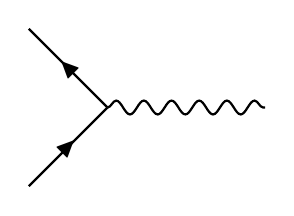
\begin{tikzpicture}[thick]
    \draw (0,0) to node[rotate=45]{$\blacktriangle$} (1,-1);
    \draw (1,-1) to node[rotate=-45]{$\blacktriangle$} (0,-2);
    \draw [decorate, decoration=snake] (1,-1) to (3,-1);
  \end{tikzpicture}
\] also gives rise to all the division algebras! (Here I've drawn the
usual picture of a spinor particle and a spinor antiparticle
annihilating to form a vector boson: this is a physics application of
the map \(m\).)

Another crucial part of the super-Poincare algebra is the action of the
Lorentz Lie algebra on spinors. Again, this has a Euclidean analogue,
where the Lie algebra of the Lorentz group gets replaced by that of the
rotation group. In \(n\) dimensions, we thus get an action
\[\mathfrak{so}(n) \times S \to S\] which we can also dualize to get a
map \[S \times S \to \mathfrak{so}(n).\] Of course, we also have the Lie
bracket
\[\mathfrak{so}(n) \times \mathfrak{so}(n) \to \mathfrak{so}(n).\] So
it's natural to ask: can we use all three of these maps to define a Lie
bracket on the direct sum of \(\mathfrak{so}(n)\) and the spinor space
\(S\)?

And the answer is: yes, but only if \(n = 9\). Then we get the
exceptional Lie algebra \(\mathrm{F}_4\).

Spurred on by our success, we can ask: what if we use right-handed
spinors instead? If we restrict the above maps to right-handed spinors,
can we define a Lie bracket on the direct sum of \(\mathfrak{so}(n)\)
and the space \(S_+\)?

And the answer is: yes, but only if \(n = 16\). Then we get the
exceptional Lie algebra \(\mathrm{E}_8\).

And then we ask: can we get the other exceptional Lie algebras by some
variant of this trick?

And the answer is: yes, at least for \(\mathrm{E}_6\) and
\(\mathrm{E}_7\).

If \(n = 10\), the spinor space \(S\) is naturally a complex vector
space, so \(\mathfrak{u}(1)\) acts on it. Using this and the above maps,
we can make the direct sum of \(\mathfrak{so}(10)\), \(S\) and
\(\mathfrak{u}(1)\) into a Lie algebra, which turns out to be
\(\mathrm{E}_6\).

If \(n = 12\), the right-handed spinor space \(S_+\) is naturally a
quaternionic vector space, so \(\mathfrak{su}(2)\) acts on it. Using
this and the above maps, we can make the direct sum of
\(\mathfrak{so}(12)\), \(S_+\) and \(\mathfrak{su}(2)\) into a Lie
algebra, which turns out to be \(\mathrm{E}_7\).

In short, we have the following story:

\begin{quote}
natural maps involving vectors and spinors give: - \(\mathbb{R}\) in
dimension 1 - \(\mathbb{C}\) in dimension 2 - \(\mathbb{H}\) in
dimension 4 - \(\mathbb{O}\) in dimension 8

natural maps involving \(\mathfrak{so}(n)\) and spinors give: -
\(\mathrm{F}_4\) in dimension 9 - \(\mathrm{E}_6\) in dimension 10 -
\(\mathrm{E}_7\) in dimension 12 - \(\mathrm{E}_8\) in dimension 16
\end{quote}

And you'll note that the dimensions in the second list are 8 more than
the corresponding dimensions in the first list. This is no coincidence!
It has to do with the octonions. But I'm too tired to explain that
now\ldots.

Anyway, my main point was just that the natural maps involving
rotation/boost generators (i.e.~the Lorentz Lie algebra, or rotation Lie
algebra), translation generators (i.e.~vectors) and supertranslation
generators (i.e.~spinors) are the essential ingredient for constructing:

\begin{enumerate}
\def\labelenumi{\alph{enumi})}
\item
  the super-Poincare algebra
\item
  the division algebras \(\mathbb{R}\), \(\mathbb{C}\), \(\mathbb{H}\)
  and \(\mathbb{O}\)
\item
  the exceptional Lie algebras \(\mathrm{F}_4\), \(\mathrm{E}_6\),
  \(\mathrm{E}_7\) and \(\mathrm{E}_8\)
\end{enumerate}

So it's not really odd to expect relations between these three things!

Of course, I've shown how items b) and c) are related to rotations,
spinors and vectors in Euclidean space, while item a) is related to
rotations/boosts, spinors and vectors in Minkowski spacetime. To round
off the picture, I'd have to describe the relation between spinors in
n-dimensional Euclidean space to spinors in \((n+2)\)-dimensional
Minkowski spacetime. It's this relation that gives the isomorphisms \[
  \begin{gathered}
    \mathfrak{so}(2,1) = \mathfrak{sl}(2,\mathbb{R})
  \\\mathfrak{so}(3,1) = \mathfrak{sl}(2,\mathbb{C})
  \\\mathfrak{so}(5,1) = \mathfrak{sl}(2,\mathbb{H})
  \\\mathfrak{so}(9,1) = \mathfrak{sl}(2,\mathbb{O})
  \end{gathered}
\] which I mentioned already in \protect\hyperlink{week104}{``Week
104''}. This is what lets us write down the super-Yang-Mills Lagrangians
and superstring Lagrangians in spacetimes of dimension 3, 4, 6, and 10
--- i.e., 2 more than the magic numbers 1, 2, 4, and 8. Adding 8, we can
guess there should also be fun stuff in spacetimes of dimensions 11, 12,
14 and 18, related to \(\mathrm{F}_4\), \(\mathrm{E}_6\),
\(\mathrm{E}_7\) and \(\mathrm{E}_8\), respectively. Is this true? Is
the 11d case related to 11d supergravity --- or M-theory? I don't know.



\hypertarget{week160}{%
\section{November 20, 2000}\label{week160}}

Anyone who grew up on science fiction in the 1960s probably read a bunch
about adventures on strange planets, and dreamt of our future in space.
At least I did. Asimov, Clarke, Heinlein\ldots{} they helped get me
interested in science, but they also painted a romantic vision of human
destiny. Only later did it become clear that \emph{for now}, the real
adventures will come from the microscopic realm: from applications of
integrated circuits, biotechnology, nanotechnology, and the like. When
you're trying to have lots of fun in a hurry, the speed limit is the
speed of light --- and this makes interstellar travel a drag.

Nonetheless, when you imbibe a romantic dream in childhood, it can be
hard to shake it it as an adult. So I still like to read about strange
planets, even if know rationally that I can have more fun at home.

So --- let me start by talking about a world where it might rain
methane!

\begin{enumerate}
\def\labelenumi{\arabic{enumi})}
\item
  Ralph D. Lorenz, ``The weather on Titan'', \emph{Science} \textbf{290}
  (October 20, 2000), 467--468.

  Caitlin A. Griffith, Joseph L. Hall and Thomas R. Geballe, ``Detection
  of daily clouds on Titan'', \emph{Science} \textbf{290} (October 20,
  2000), 509--513.
\end{enumerate}

Titan is the largest moon of Saturn, and it's the only moon in our solar
system with a significant atmosphere. Its atmosphere is mostly nitrogen,
with a surface pressure 1.5 times that of the air pressure here on
Earths' surface. However, there is also a fair amount of methane, and
even some ethane. At the surface of Titan, it's cold enough for these
compounds to liquefy. People have even seen what look like pitch-black
oceans of hydrocarbon compounds, hundreds of kilometers in size!

However, 14 kilometers or more from the surface, it gets cold enough for
methane to freeze. And the news is that recently Caitlin Griffith et al
have spotted things that look like methane clouds. Compared to Earth,
which is usually 30 percent covered with clouds, the cloud cover on
Titan seems spotty. There's not really enough methane for lots of
clouds. But there may be rain! The drops would be larger than
terrestrial raindrops, and fall slowly in the gravity of Titan, which is
like that of our moon. Since the near-surface atmosphere usually has a
relative humidity of at most 60\%, the drops would tend to evaporate
before hitting the ground. (I've seen a similar thing in New Mexico.)
However, in a big rainstorm the evaporation of the first drops might
elevate the humidity to the point where later drops could reach the
surface. So there might even be erosion on the surface of Titan. With
any luck, the Cassini spacecraft will arrive at Saturn in 2004 and make
about 40 flybys of Titan in the following 4 years, getting a good look
at this stuff.

Now for a crazy speculation of my own. Once upon a time James Lovelock
argued that you could tell there was life on earth simply by noting that
the atmosphere contains lots of oxygen, despite the fact that oxygen is
highly reactive. This means the atmosphere is far from equilibrium. Yet
the percentage of oxygen in the atmosphere has remained fairly constant
for long periods of time! So presumably there must be some homeostatic
mechanism at work to keep it constant. Only life --- he argued --- could
be responsible! Conversely, Lovelock guessed there is not life on Mars,
because its atmosphere \emph{is} in equilibrium.

Now, the methane in Titan's atmosphere is dissociated by sunlight, and
this process is irreversible, since the resulting hydrogen flies off
into space. At the rate this happens, the entire methane content of the
atmosphere would be destroyed in only 10 million years if it were not
renewed somehow. In the first article cited above, the author writes:
``For the methane we see today not to be a bizarre fluke, it must be
continuously resupplied from a surface reservoir or by cryovolcanism
(that is, volcanism where the molten `rock' is just ice).'' And this
made me wonder: where is Lovelock when we need him? Maybe \emph{life} is
responsible for this out-of-equilibrium condition.

Or maybe not. After all, it really could be something else.

Next: a world where it might rain diamonds!

\begin{enumerate}
\def\labelenumi{\arabic{enumi})}
\setcounter{enumi}{1}
\item
  Richard A. Kerr, ``Neptune may crush methane into diamonds'',
  \emph{Science} \textbf{286} (October 1, 1999), 25.

  Laura Robin Benedetti, Jeffrey H. Nguyen, Wendell A. Caldwell,
  Hongjian Liu, Michael Kruger, and Raymond Jeanloz, ``Dissociation of
  \(\mathrm{CH}_4\) at high pressures and temperatures: diamond
  formation in giant planet interiors?'', \emph{Science} \textbf{286}
  (October 1, 1999), 100--102.
\end{enumerate}

The atmosphere of Neptune is believed to contain lots of methane when
you go 4000 kilometers or more beneath the cloud tops. And Neptune ain't
no measly moon: it's a gas giant, so the atmospheric pressure becomes
enormous as you go further in. Recently, people have been compressing
methane under ridiculously high pressures, using techniques too fiendish
to describe here. At sufficiently high pressures, it releases hydrogen
and turns into diamond crystals! --- together with lots of other crud,
like ethane and acetylene. This could happen in Neptune at a depth of
about 7000 kilometers below the cloud tops, where the pressure reaches
500,000 times that of the Earth's atmosphere. So in fact, there could be
a steady rain of diamond crystals on Neptune! By the way, all these
Science articles are available for free online here:

\begin{enumerate}
\def\labelenumi{\arabic{enumi})}
\setcounter{enumi}{2}
\tightlist
\item
  Science Magazine, \texttt{http://www.sciencemag.org/search.dtl}
\end{enumerate}

I also want to say a bit about spin foams. Papers continue to come out
on this subject:

\begin{enumerate}
\def\labelenumi{\arabic{enumi})}
\setcounter{enumi}{3}
\tightlist
\item
  Alejandro Perez and Carlo Rovelli, ``A spin foam model without bubble
  divergences'', available as
  \href{https://arxiv.org/abs/gr-qc/0006107}{\texttt{gr-qc/0006107}}.
\end{enumerate}

A while ago, De Pietri, Freidel, Krasnov and Rovelli showed how to get
the Barrett-Crane model for Riemannian quantum gravity from a quantum
field theory on a product of 4 copies of \(\mathrm{SO}(4)\) --- see
\protect\hyperlink{week140}{``Week 140''}. This was based on earlier
work by Boulatov and Ooguri, who did a similar thing for \(BF\) theory.
The basic idea is to cook up a quantum field theory on a product of
copies of Lie group, with a nice Lagrangian that encodes how simplices
can stick together to form a spacetime. If you do a Feynman diagram
expansion of this quantum field theory, the Feynman diagrams can be
identified with spin foams, and the sum over Feynman diagrams becomes a
sum over spin foams.

The sum over spin foams may diverge; this paper attempts to control
those divergences. It makes some precise mathematical conjectures about
the convergence of certain sums --- mathematicians who like analysis and
representation theory should get to work on these!

\begin{enumerate}
\def\labelenumi{\arabic{enumi})}
\setcounter{enumi}{4}
\tightlist
\item
  Alejandro Perez and Carlo Rovelli, Spin foam model for Lorentzian
  general relativity, available as
  \href{https://arxiv.org/abs/gr-qc/0009021}{\texttt{gr-qc/0009021}}.
\end{enumerate}

This paper modifies the De Pietri-Freidel-Krasnov-Rovelli construction
to get the \emph{Lorentzian} Barrett-Crane model from quantum field
theory on a product of 4 copies of \(\mathrm{SO}(3,1)\).

\begin{enumerate}
\def\labelenumi{\arabic{enumi})}
\setcounter{enumi}{5}
\tightlist
\item
  Alejandro Perez and Carlo Rovelli, ``3+1 spinfoam model of quantum
  gravity with spacelike and timelike components'', available as
  \href{https://arxiv.org/abs/gr-qc/0011037}{\texttt{gr-qc/0011037}}.
\end{enumerate}

In the original Lorentzian Barrett-Crane model, spacetime is made of
4-simplices whose triangular faces are space/timelike --- in other
words, like little bits of the \(xt\) plane in Minkowski spacetime. This
model also allows \(4\)-simplices whose triangular faces are
space/spacelike --- in other words, like little bits of the \(xy\)
plane. This amounts to using a different class of irreducible unitary
representations of the Lorentz group to label the triangles.

\begin{enumerate}
\def\labelenumi{\arabic{enumi})}
\setcounter{enumi}{6}
\tightlist
\item
  Daniele Oriti and Ruth M. Williams, ``Gluing \(4\)-simplices: a
  derivation of the Barrett-Crane spin foam model for Euclidean quantum
  gravity'', available as
  \href{https://arxiv.org/abs/gr-qc/0010031}{\texttt{gr-qc/0010031}}.
\end{enumerate}

This gives an alternate derivation of the Riemannian Barrett-Crane spin
foam model starting from the Lagrangian for Riemannian general
relativity. This is good because it gives some more intuition for the
relation between classical general relativity and the spin foam approach
to quantum gravity.

Finally, if you're hopelessly confused about spin foams and other
approaches to quantum gravity, you might enjoy the following little
history of quantum gravity. It explains how many different approaches
were tried, leading up to the research directions that people pursue
now:

\begin{enumerate}
\def\labelenumi{\arabic{enumi})}
\setcounter{enumi}{7}
\tightlist
\item
  Carlo Rovelli, ``Notes for a brief history of quantum gravity'',
  presented at the 9th Marcel Grossmann Meeting in Rome, July 2000.
  Available as
  \href{https://arxiv.org/abs/gr-qc/0006061}{\texttt{gr-qc/0006061}}.
\end{enumerate}



\hypertarget{week161}{%
\section{December 10, 2000}\label{week161}}

I'm in the middle of reading this book, so I don't know how it ends yet,
but it's good:

\begin{enumerate}
\def\labelenumi{\arabic{enumi})}
\tightlist
\item
  Dava Sobel, \emph{Galileo's Daughter}, Penguin Books, London, 2000.
\end{enumerate}

Galileo had two daughters and a son with a beautiful woman whom never
married --- Marina Gamba of Venice. The son was a wastrel, and the
younger daughter was very shy, but the older daughter, Virginia, loved
Galileo very much and wrote him many letters. Of these, 124 have been
preserved, which serve as the basis of this book. At the age of 13 she
was sent to a convent, and she later became a nun. She took on the name
Suor Maria Celeste --- Sister Mary of the Heavens. Unfortunately, all of
Galileo's letters to her were destroyed by her abbess after his trial by
the Inquisition. Thus, what was really a dialog has come down to us as a
monolog. Nonetheless it is fascinating, especially since Sobel elegantly
fills in many of the holes using other sources.

Since I haven't read much about Galileo, I didn't know that this man,
often considered the father of experimental physics and telescope-aided
astronomy, was officially the ``Chief Mathematician of the University of
Pisa''. Now I can add him to my list of mathematicians who have done
good physics.

Two later figures standing on the border of math and physics are Kelvin
and Stokes:

\begin{enumerate}
\def\labelenumi{\arabic{enumi})}
\setcounter{enumi}{1}
\tightlist
\item
  David B. Wilson, \emph{Kelvin and Stokes: A Comparative Study in
  Victorian Physics}, Adam Hilger, Bristol, 1987.
\end{enumerate}

One thing I like about this book is the debunking of the popular image
of quantum mechanics and relativity as ``bolts from the blue''
shattering the complacent serenity of 19th-century physics. In physics,
the 19th century was also a century of drastic change! To quote:

\begin{quote}
Science in Victorian Britain underwent revolutionary conceptual and
institutional changes. Together, thermodynamics and the electromagnetic
theory of light, for example, transformed a bundle of only partially
linked, largely experimental sciences into a coherent, unified,
mathematical physics of energy and ether. In the 1890s one could
contemplate reducing the phenomena of matter, electricity, magnetism,
heat and light to an underlying reality of potential and kinetic energy
in an all-pervading ether. The pursuit of scientific research, largely
avocational early in the century, was a full-fledged profession by the
century's end. Science became important to university curricula, and the
universities expanded their science faculties. Institutions like the
British Association for the Advancement of Science, founded in 1831, and
Royal Society of London, reformed at mid-century, provided
organizational support for a growing community of scientists. And that
community of late-Victorian scientists resided in a community which, on
balance, was much more scientific and less religious than it had been
only two or three generations earlier. In sum late-Victorian society
endorsed the imporance of scientific knowledge and research, and
late-Victorian physics affirmed the primary significance of the ideal of
unification and the language of mathematics. In these respects, there
was an essential \emph{similarity} between late-Victorian Britain and
both the ``big science'' and the modern physics of the twentieth
century. The metamorphosis that created this state of affairs was the
context of the the careers of G. G. Stokes and William Thomson, Lord
Kelvin.
\end{quote}

Marching forwards into the 20th century, we find Einstein as another
physicist with a special tie to mathematics. Certainly he was no
mathematician, but his search for a theory of general relativity was a
curious combination of philosophical and mathematical reasoning, with
very little support from experiment. How did he really figure it out?
This book is a good place to learn the details:

\begin{enumerate}
\def\labelenumi{\arabic{enumi})}
\setcounter{enumi}{2}
\tightlist
\item
  Don Howard and John Stachel eds., \emph{Einstein and the History of
  General Relativity}, Birkhauser, Boston, 1989.
\end{enumerate}

There are a number of essays exploring the interesting period between
1912, when Einstein recognized that gravity was caused by spacetime
curvature, and 1915, when he found his field equations and used them to
compute the anomalous precession of the perihelion of Mercury. Why did
it take him so long? According to Einstein himself, ``The main reason
lies in the fact that it is not easy to free oneself from the idea that
co-ordinates must have an immediate metrical significance''.

Indeed, in 1913 he noticed that generally covariant field equations
could not uniquely determine the gravitational field generated by a
fixed mass distribution. The reason --- apart from the existence of
gravitational waves, which he was not concerned with here --- is that
one can take any solution, apply an arbitrary change of coordinates, and
get a new solution. This seemed to suggest a conflict between general
covariance and the principle that every effect should have a sufficient
cause.

Before he solved it, this conceptual problem aggravated the technical
problem of getting the right field equations: there aren't that many
good candidates for these equations if one demands general covariance,
but during the period when he distrusted this principle, Einstein and
his collaborator Grossman put a lot of work into other candidates. The
main one they tried gave Mercury an anomalous precession of 18" per
century instead of the correct value of 45" per century. Einstein only
discarded this theory in November, 1915.

On November 11th he tried a theory where the Ricci tensor was
proportional to the stress-energy tensory. On November 25th he tried a
better one, where what we now call the Einstein tensor is proportional
to the stress-energy tensor. He quickly used this to derive the correct
precession for Mercury. And so general relativity was born! In January
1916 he explained in letters to Ehrenfest and Besso how he had
reconciled general covariance with causality: two solutions of the field
equations that differ only by a change of coordinates should be regarded
as physically the same.

Now I'd like to switch to something else: a couple of emails I got. A
while back I wrote up a webpage about the end of the universe:

\begin{enumerate}
\def\labelenumi{\arabic{enumi})}
\setcounter{enumi}{3}
\tightlist
\item
  John Baez, ``The end of the universe'',
  \texttt{http://math.ucr.edu/home/baez/end.html}
\end{enumerate}

I got a lot of the numbers out of a book I bet you've already read:

\begin{enumerate}
\def\labelenumi{\arabic{enumi})}
\setcounter{enumi}{4}
\tightlist
\item
  John D. Barrow and Frank J. Tipler, \emph{The Cosmological Anthropic
  Principle}, Oxford U. Press, Oxford, 1988.
\end{enumerate}

What --- you haven't read it? Yikes! Hurry up and give it to a friend
for Christmas --- and then make them lend it to you. Regardless of what
you think about the anthropic principle, you're bound to enjoy the cool
facts this book is stuffed with! Anyway, I got an email from Barrow
saying that he's coming out with a new book. Like the previous one, it's
sure to be full of interesting things. You can tell from the title:

\begin{enumerate}
\def\labelenumi{\arabic{enumi})}
\setcounter{enumi}{5}
\tightlist
\item
  John D. Barrow, \emph{The Book of Nothing}, to be published.
\end{enumerate}

My other email was from Bert Schroer, an expert on the \(C^*\)-algebraic
approach to quantum field theory. He has written a paper about the
``AdS-CFT correspondence'' which is bound to stir up controversy:

\begin{enumerate}
\def\labelenumi{\arabic{enumi})}
\setcounter{enumi}{6}
\tightlist
\item
  Bert Schroer, ``Facts and fictions about Anti de Sitter spacetimes
  with local quantum matter'', available as
  \href{https://arxiv.org/abs/hep-th/9911100}{\texttt{hep-th/9911100}}.
\end{enumerate}

Let me just quote the beginning:

\begin{quote}
There has been hardly any problem in particle physics which has has
attracted as much attention as the problem if and in what way quantum
matter in the Anti de Sitter spacetime and the one dimension lower
conformal field theories are related and whether this could possibly
contain clues about the meaning of quantum gravity.

In more specific quantum physical terms the question is about a
conjectured (and meanwhile in large parts generically and rigorously
understood) correspondence between two quantum field theories in
different spacetime dimensions; the lower-dimensional conformal one
being the ``holographic image'' or projection of the AdS theory.

The entire globalized community of string physicists has placed this
problem in the centre of their interest and treated it as the dominating
problem of theoretical particle physics with the result that there have
been approximately around 100-150 papers per month during a good part of
1999. Even if one takes into account the increase in the number of
particle physicists during the last decades and compares it with the
relative number of participants in previous fashionable topics (the
S-matrix bootstrap, Regge theory, the \(\mathrm{SU}(6)\) --
\(\mathrm{U}(12)\) symmetric and the so-called relativistic quark
theory, to name some of them) which also led to press-conferences,
interviews and articles in the media (but not to awards and prizes), it
remains still an impressive sociological phenomenon. Just imagine
yourself working on this kind of problem and getting up every morning
turning nervously to the \texttt{hep-th} server in order to check that
nobody has beaten you to similar results. What a life in an area which
used to required a contemplative critical attitude!

This is clearly a remarkable situation in the exact sciences which
warrants an explanation. This is particularly evident to somebody old
enough to have experienced theoretical particle physics at times of
great conceptual and calculational achievements, e.g.~the derivation of
scattering theory and dispersion theory from local fields, achievements
with which the name of Harry Lehmann (to whose memory this article is
dedicated) is inexorably linked. In those times the acceptance of a
theoretical proposal in particle physics was primarily coupled to its
experimental verifiability and its conceptual standing within physics
and not yet to the beauty of its differential-geometric content. There
were also fashions, but if they did not deliver what they promised they
were allowed to die.

In the opinion of Roger Penrose, the new totalitarian attitude in
particle physics is the result of the rapid and propagandistic
communication through the new electronic media which favors speedy
calculations with no or only insufficient superficial physical
interpretation to more contemplative and not instantly profitable
conceptual investments. He cites supersymmetry and inflation cosmology
as examples of theories which achieved a kind of monopolistic dominance
despite a total lack of experimental fact (or even convincing
theoretical arguments). It seems to me that this phenomenon receives an
even stronger illustration from string theory, and I am not the only one
who thinks this way {[}here he cites a paper by I. Todorov{]}.

Leaving the final explanation of this phenomenon to historians or
sociologists of the exact sciences, I will limit myself to analyzing the
particle physics content of the so-called Anti de Sitter -- conformal
QFT correspondence from the conservative point of view of a quantum
field theorist with a 30 year professional experience who, although
having no active ambitions outside QFT, still nourishes a certain
curiosity about present activities in particle physics, e.g. string
theory or the use of noncommutative geometry. Some of the consistency
calculations one finds there are really surprising and if one could
consider them in the critical Bohr-Sommerfeld spirit as ciphers encoding
possibly new principles in fundamental physics and not as a theory (let
alone a theory of everything), these observations may have an enigmatic
use. But for this to be successful one would have to make a much more
serious attempt at confronting the new mathematical consistency
observations with local quantum physics on a more conceptual level
beyond the standard formalism. Only in this way can one be sure to
confront something new and not just a new formalism which implements the
same principles in a different way.

The AdS model of a curved spacetime has a long history as a theoretical
laboratory of what can happen with particle physics in a universe which
is the extreme opposite of globally hyperbolic in that it possesses a
self-closing time, whereas the proper de Sitter spacetime was once
considered among the more realistic models of the universe. The recent
surge of interest about AdS came from string theory and is different in
motivation and more related to the hope (or dream) to attribute a
meaning to ``Quantum Gravity'' from a string theory viewpoint.

Fortunately for the curious outsider (otherwise I would have to quit
right here), this motivation has no bearing on the conceptual and
mathematical problems posed by the would-be AdS-conformal QFT
correspondence, which turned out to be one of those properties
discovered in the setting of string theory which allow an interesting
and rigorous formulation in QFT which confirms some but not all of the
conjectured properties. The rigorous treatment however requires a
reformulation of (conformal) QFT. The standard formalism based on
pointlike ``field coordinatizations'' which underlies the Lagrangian
(and Wightman) formulations does not provide a natural setting for the
study of isomorphisms between models in different spacetime dimensions,
even though the underlying principles are the same. One would have to
introduce too many additional concepts and auxiliary tricks into the
standard framework. The important aspects in this isomorphism are
related to space and time-like (Einstein, Huyghens) causality,
localization of corresponding objects and problems of degree of freedom
counting. All these issues belong to real-time physics and in most cases
their meaning in terms of Euclidean continuation (statistical mechanics)
remains obscure; but this of course does not make them less physical.

This note is organized as follows. In the next section I elaborate on
the kinematical aspects of the
\(\mathrm{AdS}_{d+1}\)--\(\mathrm{CQFT}_d\) situation as a collateral of
the old (1974/75) compactification formalism for the
``conformalization'' of the \(d\)-dimensional Minkowski spacetime. For
this reason the seemingly more demanding problem of studying QFT
directly in AdS within a curved spacetime formalism can be bypassed. The
natural question whose answer would have led directly from
\(\mathrm{CQFT}_4\) to \(\mathrm{AdS}_5\) in the particle physics
setting (without string theory as a midwife) is: Does there exist a
quantum field theory which has the same \(\mathrm{SO}(4,2)\) symmetry
and just reprocesses the CQFT\_4 matter content in such a way that the
``conformal hamiltonian'' (the timelike generator of rotations of
conformally compactified Minkowski space) becomes the true hamiltonian?
The theory exists and is an AdS theory with a specific local matter
content computable from the CQFT matter content. The answer is unique,
but as a result of the different dimensionality one cannot describe this
unique relation between matter contents in terms of pointlike fields.
This will be treated in Section 3, where we will also compare the
content of Rehren's isomorphism with Maldacena, Witten et al conjectures
and notice some subtle but potentially serious differences. Whoever is
aware of the fact that subtle differences have often been the enigmatic
motor of progress in good physics times will not dismiss such
observations.

The last section presents some results of algebraic QFT on degrees of
freedom counting and holography. Closely connected is the idea of
``chiral scanning'', i.e.~the encoding of the full content of a higher
dimensional (massive) QFT into a finite number of copies of one chiral
theory in a carefully selected position within a common Hilbert space.
In this case the price one has to pay for this more generic holography
(light-front holography) is that some of the geometrically acting
spacetime symmetry transformations become ``fuzzy'' in the holographic
projection and some of the geometrically acting symmetries on the
holographic image are not represented by diffeomorphisms if pulled back
to the original QFT.
\end{quote}

As you can see, there is some interesting mathematical physics in here,
as well as some serious criticism of how particle physics is done these
days.

By the way, Schroer has recently written a paper about the braid group
and quantum field theory. Everyone knows how the braid group shows up in
3d quantum field theory, but this is about \emph{4d} quantum field
theory:

\begin{enumerate}
\def\labelenumi{\arabic{enumi})}
\setcounter{enumi}{7}
\tightlist
\item
  Bert Schroer, ``Braided structure in \(4\)-dimensional conformal
  quantum field theory'', available as
  \href{https://arxiv.org/abs/hep-th/0012021}{\texttt{hep-th/0012021}}.
\end{enumerate}



\hypertarget{week162}{%
\section{December 17, 2000}\label{week162}}

Since the winter solstice is coming soon, I'll start with some gift
suggestions\ldots{} for the physicist who has everything.

\begin{enumerate}
\def\labelenumi{\arabic{enumi})}
\tightlist
\item
  ``The Universe Map'', National Geographic Society, 2000, NSG \#602011.
\end{enumerate}

I've only seen a picture of this \(20\times31\) inch map, but I know I
want one! In a series of different 3d views, it shows the solar system,
nearby stars, the Milky Way, the Local Group and the observable universe
as a whole. I'll put it outside my office so my students can figure out
just where they stand in the grand scheme of things.

\begin{enumerate}
\def\labelenumi{\arabic{enumi})}
\setcounter{enumi}{1}
\tightlist
\item
  Wil Tirion and Roger W. Sinnot, \emph{Sky Atlas 2000.0}, 2nd edition,
  Cambridge U. Press, 1999.
\end{enumerate}

This is a favorite sky atlas among amateur astronomers. It comes in lots
of versions, but Kevin Kelly of Whole Earth says that the most useful is
the ``deluxe version, spiralbound''.

\begin{enumerate}
\def\labelenumi{\arabic{enumi})}
\setcounter{enumi}{2}
\tightlist
\item
  Lee Smolin, \emph{Three Roads to Quantum Gravity}, Weidenfeld and
  Nicholson, 2000.
\end{enumerate}

This is a nontechnical guide to quantum gravity and the different
approaches people have taken to this problem: string theory, loop
quantum gravity, and the more radical lines of thought pursued by people
whom Smolin calls ``the true heroes of quantum gravity'', like Alain
Connes, David Finkelstein, Chris Isham, Roger Penrose and Raphael
Sorkin. I haven't gotten ahold of this book, so I can't describe it in
detail yet, but it should be lots of fun.

That's enough gift suggestions. Now I want to talk about Jordan algebras
and how they show up in projective geometry, quantum logic, special
relativity and so on. I'll start by reminding you of some stuff from
\protect\hyperlink{week106}{``Week 106''} and
\protect\hyperlink{week145}{``Week 145''}. Then I'll charge ahead and
show you how a Jordan algebra built from the octonions is related to
\(10\)-dimensional Minkowski spacetime\ldots.

Projective geometry is a venerable subject that has its origins in the
study of perspective by Renaissance painters. As seen by the eye, any
pair of parallel lines --- e.g., train tracks --- appear to meet at a
``point at infinity''. Furthermore, when you change your viewpoint,
distances and angles appear to change, but points remain points and
lines remain lines. This suggests a modification of Euclidean plane
geometry based on a set of points, a set of lines, and relation whereby
a point ``lies on'' a line, satisfying the following axioms:

\begin{enumerate}
\def\labelenumi{\Alph{enumi})}
\item
  For any two distinct points, there is a unique line on which they both
  lie.
\item
  For any two distinct lines, there is a unique point which lies on both
  of them.
\item
  There exist four points, no three of which lie on the same line.
\item
  There exist four lines, no three of which have the same point lying on
  them.
\end{enumerate}

Any structure satisfying these axioms is called a ``projective plane''.
But projective geometry is also interesting in higher dimensions. One
can define a ``projective space'' by the following axioms:

\begin{enumerate}
\def\labelenumi{\Alph{enumi})}
\item
  For any two distinct points \(p\) and \(q\), there is a unique line
  \(pq\) on which they both lie.
\item
  For any line, there are at least three points lying on this line.
\item
  If \(a,b,c,d\) are distinct points and there is a point lying on both
  \(ab\) and \(cd\), then there is a point lying on both \(ac\) and
  \(bd\).
\end{enumerate}

Given a projective space and a set \(S\) of points in this space, we
define the ``span'' of \(S\) to be the set of all points lying on lines
\(ab\) where \(a,b\) are distinct points in \(S\). The ``dimension'' of
a projective space is defined to be one less than the smallest number of
points that span the whole space. As you would hope, a \(2\)-dimensional
projective space is the same thing as a projective plane! It's a fun
exercise to show this straight from the above axioms. If you give up,
read this book:

\begin{enumerate}
\def\labelenumi{\arabic{enumi})}
\setcounter{enumi}{3}
\tightlist
\item
  Lynn E. Garner, \emph{An Outline of Projective Geometry}, North
  Holland, New York, 1981.
\end{enumerate}

How can we get our hands on some projective spaces? Well, if
\(\mathbb{K}\) is any field, there is an \(n\)-dimensional projective
space called \(\mathbb{KP}^n\) where the points are lines through the
origin in \(\mathbb{K}^{n+1}\), the lines are planes through the origin
in \(\mathbb{K}^{n+1}\), and the relation of ``lying on'' is inclusion.
The example relevant to perspective is the real projective plane,
\(\mathbb{RP}^2\). But it's good to follow Polya's advice:

\begin{quote}
``Be wise --- generalize!''
\end{quote}

and study \(\mathbb{KP}^n\) for any field and any \(n\). In fact, we can
define \(\mathbb{KP}^n\) even when \(\mathbb{K}\) is a mere ``skew
field'': a ring such that every nonzero element has a left and right
multiplicative inverse. We just need to be a bit careful about defining
lines and planes through the origin in \(\mathbb{K}^{n+1}\). To do this,
we just take a line through the origin to be any set
\[L = {ax \mid a\in\mathbb{K}}\] where \(x\) is nonzero element of
\(\mathbb{K}^{n+1}\), and take a plane through the origin to be any set
\[P = {ax + by \mid a,b\in\mathbb{K}}\] where \(x,y\) are elements of
\(\mathbb{K}^{n+1}\) such that \(ax + by = 0\) implies \(a\) and \(b\)
are zero.

Around now, you might be wondering whether \emph{every} projective
\(n\)-space is of the form \(\mathbb{KP}^n\) for some skew field
\(\mathbb{K}\). If so, you must have forgotten
\protect\hyperlink{week145}{``Week 145''}, where I gave the answer: yes,
but only if \(n>2\). Projective planes are more subtle! A projective
plane comes from a skew field if and only if it satisfies an extra
axiom, the ``axiom of Desargues''. I described this axiom in
\protect\hyperlink{week145}{``Week 145''} so I won't do it again here.
The main point is that a projective plane coming from a skew field has
some extra geometrical properties that a ``non-Desarguesian'' projective
plane will not.

Projective geometry was very fashionable in the 1800s, with such
worthies as Poncelet, Brianchon, Steiner and von Staudt making important
contributions. Later it was overshadowed by other forms of geometry.
However, work on the subject continued, and in 1933 Ruth Moufang
constructed a remarkable example of a non-Desarguesian projective plane
using the octonions:

\begin{enumerate}
\def\labelenumi{\arabic{enumi})}
\setcounter{enumi}{4}
\tightlist
\item
  Ruth Moufang, ``Alternativkoerper und der Satz vom vollstaendigen
  Vierseit'', \emph{Abhandlungen Math. Sem. Hamburg} \textbf{9}, (1933),
  207--222.
\end{enumerate}

It turns out that this projective plane deserves the name
\(\mathbb{OP}^2\), where \(\mathbb{O}\) stands for the octonions.

The 1930s also saw the rise of another reason for interest in projective
geometry: quantum mechanics! Quantum theory is distressingly different
from the classical Newtonian physics we have learnt to love. In
classical mechanics, observables are described by real-valued functions.
In quantum mechanics, they are often described by hermitian
\(n\times n\) complex matrices. In both cases, observables are closed
under addition and multiplication by real scalars. However, in quantum
mechanics, observables do not form an associative algebra. Still, one
can raise an observable to any power, and from squaring one can define a
commutative product:
\[x \circ y = \frac12[(x+y)^2 - x^2 - y^2] = \frac12(xy + yx)\] This
product is not associative, but it satisfies the weaker identity
\[x\circ (y\circ x^2) = (x\circ y)\circ x^2\] In 1932, Pascual Jordan
attempted to understand this situation better by isolating the bare
minimum axioms that an ``algebra of observables'' should satisfy:

\begin{enumerate}
\def\labelenumi{\arabic{enumi})}
\setcounter{enumi}{5}
\tightlist
\item
  Pascual Jordan, ``Ueber eine Klasse nichtassociativer hyperkomplexer
  Algebren'', \emph{Nachr. Ges. Wiss. Goettingen} (1932), 569--575.
\end{enumerate}

He invented the definition of what is now called a ``formally real
Jordan algebra'': a commutative (but not necessarily associative) unital
algebra over the real numbers such that:
\[x\circ (y\circ x^2) = (x\circ y)\circ x^2\] and also:
\[[a^2 + b^2 + c^2 + \ldots = 0] \implies [a = b = c = \ldots = 0].\]
The last condition gives our algebra a partial ordering: if we say that
\(x\) is ``less than or equal to'' \(y\) when the element \(y-x\) is a
sum of squares, this condition says that if \(x\) is less than or equal
to \(y\) and \(y\) is less than or equal to \(x\), then \(x = y\). If we
drop this last condition, we get the definition of what is now called a
``Jordan algebra''.

In 1934, one year after Moufang published her paper on
\(\mathbb{OP}^2\), Jordan published a paper with von Neumann and Wigner
classifying all formally real Jordan algebras:

\begin{enumerate}
\def\labelenumi{\arabic{enumi})}
\setcounter{enumi}{6}
\tightlist
\item
  Pascual Jordan, John von Neumann, Eugene Wigner, ``On an algebraic
  generalization of the quantum mechanical formalism'', \emph{Ann.
  Math.} \textbf{35} (1934), 29--64.
\end{enumerate}

Their classification is nice and succinct. An ``ideal'' in the Jordan
algebra \(A\) is a subspace \(B\) such that if \(b\) is in \(B\),
\(a\circ b\) lies in \(B\) for all \(a\) in \(A\). A Jordan algebra
\(A\) is ``simple'' if its only ideals are \(\{0\}\) and \(A\) itself.
Every formally real Jordan algebra is a direct sum of simple ones. The
simple formally real Jordan algebras consist of 4 infinite families and
one exception:

\begin{itemize}
\tightlist
\item
  The algebra of \(n\times n\) self-adjoint real matrices with the
  product \[x\circ y = \frac12(xy + yx).\]
\item
  The algebra of \(n\times n\) self-adjoint complex matrices with the
  product \[x\circ y = \frac12(xy + yx).\]
\item
  The algebra of \(n\times n\) self-adjoint quaternionic matrices with
  the product \[x\circ y = \frac12(xy + yx).\]
\item
  The algebra \(\mathbb{R}^n\oplus\mathbb{R}\) with the product
  \[(v,a) o (w,b) = (aw + bv, \langle v,w\rangle + ab)\] where
  \(\langle v,w\rangle\) is the usual inner product of vectors in
  \(\mathbb{R}^n\). This sort of Jordan algebra is called a ``spin
  factor''.
\item
  The algebra of \(3\times3\) self-adjoint octonionic matrices with the
  product \[x\circ y = \frac12(xy + yx).\] This is called the
  ``exceptional Jordan algebra''.
\end{itemize}

This classification raises some obvious questions. Why does nature
prefer the Jordan algebras \(h_n(\mathbb{C})\) over all the rest? Or
does it? Could the other Jordan algebras --- even the exceptional one
--- have some role to play in quantum physics? Despite much research,
these questions remain unanswered to this day.

The paper by Jordan, von Neumann and Wigner appears to have been
uninfluenced by Moufang's discovery of \(\mathbb{OP}^2\), but in fact
the two are related! A ``projection'' in a formally real Jordan algebra
is defined to be an element \(p\) with \(p^2 = p\). In the usual case of
\(h_n(\mathbb{C})\), these correspond to hermitian matrices with
eigenvalues \(0\) and \(1\), so they are used to describe observables
that assume only two values --- e.g., ``true'' and ``false''.

This suggests treating projections in a formally real Jordan algebra as
propositions in a kind of ``quantum logic''. The partial order helps us
do this: given projections \(p\) and \(q\), we say that \(p\)
``implies'' \(q\) if \(p\) is less than or equal to \(q\). We can then
go ahead and define ``and'', ``or'' and ``not'' in this context, and
most of the familiar rules of Boolean logic continue to hold. However,
we no longer have the distributive laws: \[
  \begin{gathered}
    \mbox{$p$ and ($q$ or $r$) = ($p$ and $q$) or ($p$ and $r$)}
  \\\mbox{$p$ or ($q$ and $r$) = ($p$ or $r$) and ($q$ or $r$)}
  \end{gathered}
\] The failure of these distributive laws is the hallmark of quantum
logic.

Now, the relation between Jordan algebras and quantum logic is already
interesting in itself:

\begin{enumerate}
\def\labelenumi{\arabic{enumi})}
\setcounter{enumi}{7}
\tightlist
\item
  G. Emch, \emph{Algebraic Methods in Statistical Mechanics and Quantum
  Field Theory}, Wiley-Interscience, New York, 1972.
\end{enumerate}

\ldots{} but the real fun starts when we note that projections in the
Jordan algebra of \(n\times n\) self-adjoint complex matrices correspond
to subspaces of \(\mathbb{C}^n\). This sets up a relationship to
projective geometry, since the projections onto \(1\)-dimensional
subspaces correspond to points in \(\mathbb{CP}^n\), while the
projections onto \(2\)-dimensional subspaces correspond to lines. Even
better, we can work out the dimension of a subspace \(V\) from the
corresponding projection \(p\colon\mathbb{C}^n\to V\) using only the
partial order on projections: \(V\) has dimension \(d\) iff the longest
chain of distinct projections \[p_0 < p_1 < \ldots < p_i = p\] has
length \(i = d\). In fact, we can use this to define the ``dimension''
of any projection in \emph{any} formally real Jordan algebra. We can
then try to construct a projective space whose points are the
\(1\)-dimensional projections and whose lines are the \(2\)-dimensional
projections, with the relation of ``lying on'' given by the partial
order in our Jordan algebra.

If we try this starting with the Jordan algebra of \(n\times n\)
self-adjoint matrices with real, complex or quaternionic entries, we
succeed when \(n\) is \(2\) or more --- and we obtain the projective
spaces \(\mathbb{RP}^n\), \(\mathbb{CP}^n\) and \(\mathbb{HP}^n\),
respectively. If we try this starting with the spin factor
\(\mathbb{R}^n\oplus\mathbb{R}\) we succeed when \(n\) is \(2\) or more
--- and we obtain a series of 1-dimensional projective spaces related to
Minkowskian geometry, which I'll talk about in a minute. Finally, in
1949 Jordan discovered that if we try this construction starting with
the exceptional Jordan algebra, we get the projective plane discovered
by Ruth Moufang --- \(\mathbb{OP}^2\)!

\begin{enumerate}
\def\labelenumi{\arabic{enumi})}
\setcounter{enumi}{8}
\tightlist
\item
  Pascual Jordan, ``Ueber eine nicht-desarguessche ebene projektive
  Geometrie'', \emph{Abhandlungen Math. Sem. Hamburg} \textbf{16}
  (1949), 74--76.
\end{enumerate}

Physicists have tried for a long time to find some use for the quantum
logic corresponding to the exceptional Jordan algebra. So far they have
not succeeded. Jordan hoped this stuff would be related to nuclear
physics. Feza Gursey and Murat Gunaydin hoped it was related to quarks,
since \(3\times3\) hermitian octonionic matrices should describe
observables in some 3-state quantum system:

\begin{enumerate}
\def\labelenumi{\arabic{enumi})}
\setcounter{enumi}{9}
\item
  Murat Gunaydin and Feza Gursey, ``An octonionic representation of the
  Poincare group'', \emph{Lett. Nuovo Cim.} \textbf{6} (1973), 401--406.
\item
  Murat Gunaydin and Feza Gursey, ``Quark structure and octonions'',
  \emph{Jour. Math. Phys.} \textbf{14} (1973), 1615--1667.
\item
  Murat Gunaydin and Feza Gursey, ``Quark statistics and octonions'',
  \emph{Phys. Rev.} \textbf{D9} (1974), 3387--3391.
\item
  Murat Gunaydin,
  \(Octonionic Hilbert spaces, the Poincare group and \mathrm{SU}(3)\),
  \emph{Jour. Math. Phys.} \textbf{17} (1976), 1875--1883.
\item
  M. Gunaydin, C. Piron and H. Ruegg, ``Moufang plane and octonionic
  quantum mechanics'', \emph{Comm. Math. Phys.} \textbf{61} (1978),
  69--85.
\end{enumerate}

Alas, these ideas never quite worked out, so most physicists discarded
the exceptional Jordan algebra as a lost cause.

However, the exceptional Jordan algebra is secretly related to string
theory, so there's a sense in which it's still lurking in the collective
subconscious. Now, you probably want me to explain this, but I'm not
ready to. So I won't say what \(3\times3\) hermitian octonionic matrices
have to do with string theory. If you want to know that, read these:

\begin{enumerate}
\def\labelenumi{\arabic{enumi})}
\setcounter{enumi}{14}
\item
  E. Corrigan and T. J. Hollowood, ``The exceptional Jordan algebra and
  the superstring'', \emph{Commun. Math. Phys.} \textbf{122} (1989),
  393. Also available at
  \href{http://projecteuclid.org/DPubS?service=UI\&version=1.0\&verb=Display\&handle=euclid.cmp/1104178468}{\texttt{http://projecteuclid.org/}}
\item
  E. Corrigan and T. J. Hollowood, ``A string construction of a
  commutative nonassociative algebra related to the exceptional Jordan
  algebra'', \emph{Phys. Lett.} \textbf{B203} (1988), 47.
\item
  G. Sierra, ``An application of the theories of Jordan algebras and
  Freudenthal triple systems to particles and strings'', \emph{Class.
  Quant. Grav.} \textbf{4} (1987), 227.
\end{enumerate}

Instead, I'll just say what \(2\times2\) hermitian octonionic matrices
have to do with \(10\)-dimensional Minkowski spacetime. Since
superstrings live in 10 dimensions, that's at least a start.

First, we need to think about spin factors.

In case you forgot, spin factors were the fourth infinite family of
simple formally real Jordan algebras on my list up there. I gave a
lowbrow definition of these guys, but now let's try a highbrow one.
Given an \(n\)-dimensional real inner product space \(V\), the ``spin
factor'' \(J(V)\) is the Jordan algebra generated by \(V\) with the
relations \[v\circ w = \langle v,w\rangle\] This should remind you of
the definition of a Clifford algebra, and indeed, they're related ---
they have the same representations! This sets up a connection to
spinors, which is why these Jordan algebras are called ``spin factors''.

But anyway: if you think about it a while, you'll see that \(J(V)\) is
isomorphic to the direct sum \(V\oplus\mathbb{R}\) equipped with the
product \[(v,a)\circ(w,b) = (aw + bv, \langle v,w\rangle + ab)\] which
is basically the lowbrow definition of a spin factor.

Though Jordan algebras were invented to study quantum mechanics, the
spin factors are also deeply related to special relativity: we can think
of \(J(V) = V\oplus\mathbb{R}\) as ``Minkowski spacetime'', with \(V\)
as space and \(\mathbb{R}\) as time. The reason is that \(J(V)\) is
naturally equipped with a dot product:
\[(v,a)\cdot(w,b) = \langle v,w\rangle - ab\] which is just the usual
Minkowski metric in slight disguise. This makes it tempting to borrow an
idea from special relativity and define the ``lightcone'' to consist of
all nonzero \(x\) in \(J(V)\) with \[x\cdot x = 0\] A \(1\)-dimensional
subspace of \(J(V)\) spanned by an element of the lightcone is called a
``light ray'', and the space of all light rays is called the ``heavenly
sphere'' \(S(V)\). We can identify the heavenly sphere with the sphere
of unit vectors in \(V\), since every light ray is spanned by an element
of \(J(V)\) of the form \((v,1)\) where \(v\) is a unit vector in \(V\).

What's the physical meaning of the heavenly sphere? Well, if you were a
resident of the spacetime \(J(V)\) and gazed up at the sky at night, the
stars would seem to lie on this sphere. If you took off in a spaceship
and whizzed along at close to the speed of light, all the constellations
would look distorted, but all \emph{angles} would be preserved, since
the Lorentz group acts as conformal transformations of the heavenly
sphere.

Now, when \(V\) is at least \(2\)-dimensional, we can build a projective
space from \(J(V)\) using the construction I described for any simple
formally real Jordan algebra. If we do this, what do we get?

Well, you can easily check that aside from the elements \(0\) and \(1\),
all projections in \(J(V)\) are of the form \(p = \frac12(v,1)\) where v
is a unit vector in V. These projections will be the points of our
projective space, but as we've seen, they also correspond to points of
the heavenly sphere. So our projective space is really just the heavenly
sphere! This is cool, because it means points on the heavenly sphere can
also be thought of as \emph{propositions} in a certain sort of quantum
logic.

Now, what does this have to do with the exceptional Jordan algebra?
Well, we have to sneak up carefully on this wild beast, so first let's
think about a smaller Jordan algebra: the \(2\times2\) hermitian
octonionic matrices. In fact, we can kill four birds with one stone, and
think about \(2\times2\) hermitian matrices with entries in any
\(n\)-dimensional normed division algebra, say \(\mathbb{K}\). There are
not that many normed division algebras, so I really just mean:

\begin{itemize}
\tightlist
\item
  the real numbers, \(\mathbb{R}\), if \(n = 1\),
\item
  the complex numbers, \(\mathbb{C}\), if \(n = 2\),
\item
  the quaternions, \(\mathbb{H}\), if \(n = 4\),
\item
  the octonions, \(\mathbb{O}\), if \(n = 8\).
\end{itemize}

The space \(\mathrm{h}_2(\mathbb{K})\) of hermitian \(2\times2\)
matrices with entries in \(\mathbb{K}\) is a Jordan algebra with the
product \[x\circ y = \frac12(xy + yx)\] Moreover, this Jordan algebra is
secretly a spin factor! There is an isomorphism
\[f\colon \mathrm{h}_2(\mathbb{K}) \to J(\mathbb{K}\oplus\mathbb{R}) = \mathbb{K}\oplus\mathbb{R}\oplus\mathbb{R}\]
which sends the hermitian matrix \[
  \left(
    \begin{array}{cc}
      a+b&k
    \\k^*&a-b
    \end{array}
  \right)
\] to the element \((k,b,a)\) in \(K\oplus\mathbb{R}\oplus\mathbb{R}\).

Furthermore, the determinant of matrices in \(\mathrm{h}_2(\mathbb{K})\)
is just the Minkowski metric in disguise, since the determinant of \[
  \left(
    \begin{array}{cc}
      a+b&k
    \\k^*&a-b
    \end{array}
  \right)
\] is \[a^2-b^2-\langle k,k\rangle.\]

These facts have a number of nice consequences. First of all, since the
Jordan algebras \(J(\mathbb{K}\oplus\mathbb{R})\) and
\(\mathrm{h}_2(\mathbb{K})\) are isomorphic, so are their associated
projective spaces. We have seen that the former space is the heavenly
sphere \(S(\mathbb{K}\oplus\mathbb{R})\); unsurprisingly, the latter is
the projective line \(\mathbb{KP}^1\). It follows that these are the
same! This shows that:

\begin{itemize}
\tightlist
\item
  \(\mathrm{h}_2(\mathbb{R})\) is 3d Minkowski spacetime, and
  \(\mathbb{RP}^1\) is the heavenly sphere \(S^1\);
\item
  \(\mathrm{h}_2(\mathbb{C})\) is 4d Minkowski spacetime, and
  \(\mathbb{CP}^1\) is the heavenly sphere \(S^2\);
\item
  \(\mathrm{h}_2(\mathbb{H})\) is 6d Minkowski spacetime, and
  \(\mathbb{HP}^1\) is the heavenly sphere \(S^4\);
\item
  \(\mathrm{h}_2(\mathbb{O})\) is 10d Minkowski spacetime, and
  \(\mathbb{OP}^1\) is the heavenly sphere \(S^8\).
\end{itemize}

Secondly, it follows that the determinant-preserving linear
transformations of \(\mathrm{h}_2(\mathbb{K})\) form a group isomorphic
to \(\mathrm{O}(n+1,1)\). How can we find some transformations of this
sort? For \(\mathbb{K}=\mathbb{R}\), it's easy: when \(g\) lies in
\(\mathrm{SL}(2,\mathbb{R})\) and \(x\) is in
\(\mathrm{h}_2(\mathbb{R})\), we have \(gxg^*\) in
\(\mathrm{h}_2(\mathbb{R})\) again, and \[\det(gxg*) = \det(x).\] This
gives a homomorphism from \(\mathrm{SL}(2,\mathbb{R})\) to
\(\mathrm{O}(2,1)\). It's easy to see that this makes
\(\mathrm{SL}(2,\mathbb{R})\) into a double cover of the Lorentz group
\(\mathrm{SO}_0(2,1)\). The exact same construction works for
\(\mathbb{K}=\mathbb{C}\), so \(\mathrm{SL}(2,\mathbb{C})\) is a double
cover of the Lorentz group \(\mathrm{SO}_0(3,1)\) --- which you probably
knew already, if you made it this far!

For the other two normed division algebras the above calculation
involving determinants breaks down, and it even becomes tricky to define
the group \(\mathrm{SL}(2,\mathbb{K})\), so we'll start by working at
the Lie algebra level. We say a \(2\times2\) matrix with entries in the
normed division algebra \(\mathbb{K}\) is ``traceless'' if the sum of
its diagonal entries is zero. Any such traceless matrix acts as a
real-linear operator on \(\mathbb{K}^2\). When \(\mathbb{K}\) is
commutative and associative, the space of operators coming from
\(2\times2\) traceless matrices with entries in \(\mathbb{K}\) is closed
under commutators, but otherwise it is not, so we'll define
\(\mathfrak{sl}(2,\mathbb{K})\) to be the Lie algebra of operators on
\(\mathbb{K}^2\) \emph{generated} by operators of this form. This Lie
algebra in turn generates a Lie group of real-linear operators on
\(\mathbb{K}^2\), which we call \(\mathrm{SL}(2,\mathbb{K})\).

Now, \(\mathfrak{sl}(2,\mathbb{K})\) has an obvious representation on
\(\mathbb{K}^2\), called the ``fundamental representation''. If we
tensor this representation with its dual we get a representation of
\(\mathfrak{sl}(2,\mathbb{K})\) on the space of \(2\times2\) matrices
with entries in \(\mathbb{K}\), which is given by
\[a\colon x \mapsto ax + xa^*\] whenever \(a\) is actually a
\(2\times2\) traceless matrix with entries in \(\mathbb{K}\). Since
\(ax + xa^*\) is hermitian whenever \(x\) is, this representation
restricts to a representation of \(\mathfrak{sl}(2,\mathbb{K})\) on
\(\mathrm{h}_2(\mathbb{K})\). This in turn gives a rep of the group
\(\mathrm{SL}(2,\mathbb{K})\). A little calculation at the Lie algebra
level shows that this action of \(\mathrm{SL}(2,\mathbb{K})\) on
\(\mathrm{h}_2(\mathbb{K})\) preserves the determinant, so we have a
homomorphism \[\mathrm{SL}(2,\mathbb{K}) \to \mathrm{SO}_0(n+1,1).\]
This is two-to-one and onto, so it follows pretty easily that:

\begin{itemize}
\tightlist
\item
  \(\mathrm{SL}(2,\mathbb{R})\) is the double cover of the Lorentz group
  \(\mathrm{SO}_0(2,1)\);
\item
  \(\mathrm{SL}(2,\mathbb{C})\) is the double cover of the Lorentz group
  \(\mathrm{SO}_0(3,1)\);
\item
  \(\mathrm{SL}(2,\mathbb{H})\) is the double cover of the Lorentz group
  \(\mathrm{SO}_0(5,1)\);
\item
  \(\mathrm{SL}(2,\mathbb{O})\) is the double cover of the Lorentz group
  \(\mathrm{SO}_0(9,1)\).
\end{itemize}

and thus:

\begin{itemize}
\tightlist
\item
  \(\mathrm{SL}(2,\mathbb{R})\) acts as conformal transformations of the
  sphere \(S^1 = \mathbb{RP}^1\);
\item
  \(\mathrm{SL}(2,\mathbb{C})\) acts as conformal transformations of the
  sphere \(S^2 = \mathbb{CP}^1\);
\item
  \(\mathrm{SL}(2,\mathbb{H})\) acts as conformal transformations of the
  sphere \(S^4 = \mathbb{HP}^1\);
\item
  \(\mathrm{SL}(2,\mathbb{O})\) acts as conformal transformations of the
  sphere \(S^8 = \mathbb{OP}^1\).
\end{itemize}

In the complex case, these conformal transformations are often called
``Moebius transformations''. For more on the octonionic case, try this:

\begin{enumerate}
\def\labelenumi{\arabic{enumi})}
\setcounter{enumi}{14}
\tightlist
\item
  Corinne A. Manogue and Tevian Dray, ``Octonionic Moebius
  transformations'', \emph{Mod. Phys. Lett.} \textbf{A14} (1999)
  1243--1256, available as
  \href{https://arxiv.org/abs/math-ph/9905024}{\texttt{math-ph/9905024}}.
\end{enumerate}

To round off the story, it helps to bring in spinors:

\begin{enumerate}
\def\labelenumi{\arabic{enumi})}
\setcounter{enumi}{15}
\tightlist
\item
  Anthony Sudbery, ``Division algebras, (pseudo)orthogonal groups and
  spinors'', \emph{Jour. Phys.} \textbf{A17} (1984), 939--955.
\end{enumerate}

The fundamental rep of \(\mathrm{SL}(2,\mathbb{K})\) on \(\mathbb{K}^2\)
is secretly one of the spinor reps of the double cover of the Lorentz
group \(\mathrm{SO}_0(n+1,1)\). Moreover, we can get points on the
heavenly sphere from these spinors! This has been nicely explained by
Penrose in the complex case, but it works the same way for the other
normed division algebras. It goes like this:

Suppose \[\vert\psi\rangle = (x,y)\] is a unit spinor, i.e.~an element
of \(\mathbb{K}^2\) with norm one. Then \[
  \vert\psi\rangle\langle\psi\vert =
  \left(
    \begin{array}{cc}
      xx^*&xy^*
    \\yx^*&yy^*
    \end{array}
  \right)
\] is a projection in \(\mathrm{h}_2(\mathbb{K})\) which is not \(0\) or
\(1\) --- or in other words, a point on the heavenly sphere. If we
identify the heavenly sphere with \(\mathbb{KP}^1\), this point
corresponds to the line through the origin in \(\mathbb{K}^2\)
containing the spinor \(\vert\psi\rangle\).

To go further, I would want to say more about why this connection
between quantum logic, Lorentzian geometry, and spinors is interesting,
and what you can do with it. And then I would want to take everything
we've seen about \(\mathbb{OP}^1\) and \(\mathrm{h}_2(\mathbb{O})\) and
see how it fits inside the bigger, more interesting story of
\(\mathbb{OP}^2\) and \(\mathrm{h}_3(\mathbb{O})\). But alas, I'm
running out of steam here, so I'll just give you a little reading list
about the octonionic projective plane and the exceptional Jordan
algebra:

\begin{enumerate}
\def\labelenumi{\arabic{enumi})}
\setcounter{enumi}{19}
\item
  Hans Freudenthal, ``Zur ebenen Oktavengeometrie'', \emph{Indag. Math.}
  \textbf{15} (1953), 195--200.

  Hans Freudenthal, ``Beziehungen der \(\mathfrak{e}_7\) und
  \(\mathfrak{e}_8\) zur Oktavenebene'':

\begin{verbatim}
I, II, _Indag. Math._ **16** (1954), 218--230, 363--368.

III, IV, _Indag. Math._ **17** (1955), 151--157, 277--285.

V -- IX, _Indag. Math._ **21** (1959), 165--201, 447--474.

X, XI, _Indag. Math._ **25** (1963) 453--471, 472--487.
\end{verbatim}

  Hans Freudenthal, ``Lie groups in the foundations of geometry'',
  \emph{Adv. Math.} \textbf{1} (1964), 145--190.

  Hans Freudenthal, ``Oktaven, Ausnahmegruppen und Oktavengeometrie'',
  \emph{Geom. Dedicata} \textbf{19} (1985), 7--63.
\item
  Jacques Tits, ``Le plan projectif des octaves et les groupes de Lie
  exceptionnels'', \emph{Bull. Acad. Roy. Belg. Sci.} \textbf{39}
  (1953), 309--329.
\end{enumerate}

Jacques Tits, Le plan projectif des octaves et les groupes exceptionnels
\(\mathrm{E}_6\) et \(\mathrm{E}_7\), \emph{Bull. Acad. Roy. Belg. Sci.}
\textbf{40} (1954), 29--40.

\begin{enumerate}
\def\labelenumi{\arabic{enumi})}
\setcounter{enumi}{21}
\item
  Tonny A. Springer, ``The projective octave plane, I-II'', \emph{Proc.
  Koninkl. Akad. Wetenschap.} \textbf{A63} (1960), 74--101.

  Tonny A. Springer, ``On the geometric algebra of the octave planes,
  I-III'', \emph{Proc. Koninkl. Akad. Wetenschap.} \textbf{A65} (1962),
  413--451.
\item
  J. R. Faulkner and J. C. Ferrar, ``Exceptional Lie algebras and
  related algebraic and geometric structures'', \emph{Bull. London Math.
  Soc.} \textbf{9} (1977), 1--35.
\end{enumerate}

Finally, for a really good overview of Jordan algebras and related
things like ``Jordan pairs'' and ``Jordan triple systems'', try this:

\begin{enumerate}
\def\labelenumi{\arabic{enumi})}
\setcounter{enumi}{23}
\tightlist
\item
  Kevin McCrimmon, ``Jordan algebras and their applications'', \emph{AMS
  Bulletin} \textbf{84} (1978), 612--627.
\end{enumerate}



\hypertarget{week163}{%
\section{December 31, 2000}\label{week163}}

If you think numbers start with the number 1, you probably think the
millennium is ending now. I think it ended last year\ldots{} but either
way, now is a good time to read this book:

\begin{enumerate}
\def\labelenumi{\arabic{enumi})}
\tightlist
\item
  Georges Ifrah, \emph{The Universal History of Numbers from Prehistory
  to the Invention of the Computer}, Wiley, New York, 2000.
\end{enumerate}

On the invention of zero:

\begin{quote}
Most peoples throughout history failed to discover the rule of position,
which was discovered in fact only four times in the history of the
world. (The rule of position is the principle in which a 9, let's say,
has a different magnitude depending on whether it comes in first,
second, third\ldots{} position in a numerical expression.) The first
discovery of this essential tool of mathematics was made in Babylon in
the second millennium BCE. It was then rediscovered by the Chinese
arithmeticians at around the start of the Common Era. In the third to
fifth centuries CE, Mayan astronomers reinvented it, and in the fifth
century CE it was rediscovered for the last time, in India.

Obviously, no civilization outside of these four ever felt the need to
invent zero; but as soon as the rule of position became the basis for a
numbering system, a zero was needed. All the same, only three of the
four (the Babylonians, the Mayans, and the Indians) managed to develop
this final abstraction of number; the Chinese only acquired it through
Indian influences. However, the Babylonian and Mayan zeroes were not
conceived of as numbers, and only the Indian zero had roughly the same
potential as the one we use nowadays. That is because it is indeed the
Indian zero, transmitted to us through the Arabs together with the
number-symbols that we call Arabic numerals and which are in reality
Indian numerals, with their appearance altered somewhat by time, use and
travel.
\end{quote}

Among other things, this book has wonderful charts showing the
development of each numeral. You can see, for example, how the primitive
numeral

\begin{verbatim}
                          ____
                          ____
                          ____
\end{verbatim}

slowly evolved to our modern ``3''. Hmm --- how come this doesn't feel
like progress?

Now, I usually keep my eyes firmly focused on the beauties of nature,
but once in a millennium I feel the need to engage in some politics.
So\ldots.

In \protect\hyperlink{week155}{``Week 155''} I talked a lot about
polyhedra and their 4-dimensional generalizations, and I referred to
Eric Weisstein's online math encyclopedia since it had lots of nice
pictures. Now this website has been closed down, thanks to a lawsuit by
the people at CRC Press:

\begin{enumerate}
\def\labelenumi{\arabic{enumi})}
\setcounter{enumi}{1}
\tightlist
\item
  Frequently asked questions about the MathWorld case,
  \texttt{http://mathworld.wolfram.com/docs/faq.html}
\end{enumerate}

Weisstein published a print version of his encyclopedia with CRC press,
but now they claim to own the rights to the online version as well. So I
urge you all to remember this: \emph{when dealing with publishers, never
sign away the electronic rights on your work unless you're willing to
accept the consequences!}

For example, suppose you write a math or physics paper and put it on the
preprint archive, and then publish it in a journal. They'll probably
send you a little form to sign where you hand over the rights to this
work --- including the electronic rights. If you're like most people,
you'll sign this form without reading it. This means that if they feel
like it, they can now sue you to make you take your paper off the
preprint archive! Journals don't do this yet, but as they continue
becoming obsolete and keep fighting ever more desperately for their
lives, there's no telling what they'll do. Corporations everywhere are
taking an increasingly aggressive line on intellectual property rights
--- as the case of Weisstein shows.

So what can you do? Simple: don't agree to it. When you get this form,
cross out any sentences you refuse to agree to, put your initials by
these deletions, and sign the thing --- indicating that you agree to the
\emph{other} stuff! Keep a copy. If they complain, ask them how much
these electronic rights are worth.

Basically, I think it's time for academics to take more responsibility
about keeping their work easily accessible.

There are lots of things you can do. One of the easiest is to stop
refereeing for ridiculously expensive journals. Journal prices bear
little relation to the quality of service they provide. For example, the
Elsevier-published journal ``\emph{Nuclear Physics B}'' costs \$12,596
per year for libraries, or \$6,000 for a personal subscription. The
comparable journal ``Advances in Theoretical and Mathematical Physics''
costs \$300 for libraries or \$80 for a personal subscription --- and
access to the electronic version is free. So when Nuclear Physics B asks
me to referee manuscripts, I now say ``Sorry, I'll wait until your
prices go down.''

In fact, I no longer referee articles for any journals published by
Elsevier, Kluwer, or Gordon \& Breach. If you've looked at their prices,
you'll know why. G\&B has even taken legal action against the American
Institute of Physics, the American Physical Society, and the American
Mathematical Society for publishing information about journal prices!

\begin{enumerate}
\def\labelenumi{\arabic{enumi})}
\setcounter{enumi}{2}
\item
  Gordon and Breach et al v. AIP and APS, brief of amici curiae of the
  American Library Association, Association of Research Libraries and
  the Special Library Association,
  \texttt{http://www.arl.org/scomm/gb/amici.html}
\item
  AIP/APS prevail in suit by Gordon and Breach, G\&B to appeal,
  \texttt{http://www.arl.org/newsltr/194/gb.html}
\end{enumerate}

Of course, the ultimate solution is to support the math and physics
preprint archives, and figure out ways to decouple the refereeing
process from the distribution process.

Okay, enough politics. I was thinking about \(4\)-dimensional polytopes,
and Eric Weisstein's now-defunct website\ldots{} but what got me going
in the first place was this:

\begin{enumerate}
\def\labelenumi{\arabic{enumi})}
\setcounter{enumi}{4}
\tightlist
\item
  John Stilwell, ``The story of the 120-cell'', \emph{AMS Notices}
  \textbf{48} (January 2001), 17--24.
\end{enumerate}

The 120-cell is a marvelous \(4\)-dimensional shape with 120 regular
dodecahedra as faces. I talked about it in
\protect\hyperlink{week155}{``Week 155''}, but this article is full of
additional interesting information. For example, Henri Poincare once
conjectured that every compact 3-manifold with the same homology groups
as a 3-sphere must \emph{be} a 3-sphere. He later proved himself wrong
by finding a counterexample: the ``Poincare homology 3-sphere''. This is
obtained by identifying the opposite faces of the dodecahedron in the
simplest possible way. What I hadn't known is that the fundamental group
of this space is the ``binary icosahedral group'', \(I\). This is the
120-element subgroup of \(\mathrm{SU}(2)\) consisting of all elements
that map to rotational symmetries of the icosahedron under the
two-to-one map from \(\mathrm{SU}(2)\) to \(\mathrm{SO}(3)\). Now
\(\mathrm{SU}(2)\) is none other than the 3-sphere\ldots{} so it follows
that \(\mathrm{SU}(2)/I\) is the Poincare homology 3-sphere!

When cosmologists study the possility that universe is finite in size,
they usually assume that space is a 3-sphere. In this scenario, barring
sneaky tricks, it's likely that the universe would recollapse before
light could get all the way around the universe. But there's no strong
reason to favor this topology. Some people have checked to see whether
space is a \(3\)-dimensional torus. In such a universe, light might wrap
all the way around --- so you might see the same bright quasars by
looking in various different directions! People have looked for this
effect but not seen it. This doesn't rule out a torus-shaped universe,
but it puts a limit on how small it could be.

In fact, some physicists have even considered the possibility that space
is a Poincare homology 3-sphere! Can light go all the way around in this
case? I don't know. If so, we might see bright quasars in a pretty
dodecahedral pattern.

Amusingly, Plato hinted at something resembling this in his ``Timaeus'':

\begin{enumerate}
\def\labelenumi{\arabic{enumi})}
\setcounter{enumi}{5}
\tightlist
\item
  Plato, ``Timaeus'', translated by B. Jowett, in \emph{The Collected
  Dialogues}, Princeton U. Press, Princeton, 1969 (see line 55c).
\end{enumerate}

This dialog is one the first attempts at doing mathematical physics. In
it, the Socrates character guesses that the four elements earth, air,
water and fire are made of atoms shaped like four of the five Platonic
solids: cubes, octahedra, icosahedra and tetrahedra, respectively. Why?
Well, fire obviously feels hot because of those pointy little tetrahedra
poking you! Water is liquid because of those round little icosahedra
rolling around. Earth is solid because of those little cubes packing
together so neatly. And air\ldots{} well, ahem\ldots{} we'll get back to
you on that one.

\emph{But what about the dodecahedron?} On this topic, Plato makes only
the following cryptic remark: ``There was yet a fifth combination which
God used in the delineation of the universe with figures of animals.''

Huh??? I think this is a feeble attempt to connect the 12 sides of the
dodecahedron to the 12 signs of the zodiac. After all, lots of the signs
of the zodiac are animals. The word ``zodiac'' comes from the Greek
phrase ``zodiakos kuklos'', or ``circle of carved figures'' --- where
``zodiakos'' or ``carved figure'' is really the diminutive of ``zoion'',
meaning ``animal''. There may even be a connection between the
dodecahedron and the ``quintessence'': the fifth element, of which the
heavenly bodies were supposedly made. I know, this is all pretty weird,
but there seems to be some tantalizingly murky connection between the
dodecahedron and the heavens in Greek cosmology\ldots. so it would be
cool if space turned out to be a Poincare homology 3-sphere. But of
course, there's no reason to believe it is.

Okay, enough goofing around. Now let me talk a bit about the exceptional
Jordan algebra and the octonionic projective plane. I'll basically pick
up where I left off in \protect\hyperlink{week162}{``Week 162''} --- but
you might want to reread \protect\hyperlink{week61}{``Week 61''},
\protect\hyperlink{week106}{``Week 106''} and
\protect\hyperlink{week145}{``Week 145''} to prepare yourself for the
weirdness to come. Also, keep in mind the following three facts about
the number 3, which fit together in a spooky sort of synergy that makes
all the magic happen:

\begin{enumerate}
\def\labelenumi{\roman{enumi})}
\item
  An element of \(\mathrm{h}_3(\mathbb{O})\) is a \(3\times3\) hermitian
  matrix with octonionic entries, and thus consists of 3 octonions and 3
  real numbers: \[
     \left(
       \begin{array}{ccc}
         a&z^*&y^*
       \\z&b&x
       \\y&x^*&c
       \end{array}
     \right)
     \qquad\mbox{($a,b,c$ in $\mathbb{R}$, $x,y,z$ in $\mathbb{O}$.)}
   \]
\item
  The octonions arise naturally from ``triality'': the relation between
  the three \(8\)-dimensional irreps of \(\mathrm{Spin}(8)\), i.e.~the
  vector representation \(V_8\), the right-handed spinor representation
  \(S_8^+\), and the left-handed spinor representation \(S_8^-\).
\item
  The associative law \((xy)z = x(yz)\) involves 3 variables.
\end{enumerate}

Let's see how it goes.

First, if we take the 3 octonions in our element of
\(\mathrm{h}_3(\mathbb{O})\) and identify them with elements of the
three \(8\)-dimensional irreps of \(\mathrm{Spin}(8)\), we get
\[\mathrm{h}_3(\mathbb{O}) = \mathbb{R}^3\oplus V_8\oplus S_8^+\oplus S_8^-.\]
A little calculation then reveals a wonderful fact: while superficially
the Jordan product in \(\mathrm{h}_3(\mathbb{O})\) is built using the
structure of \(\mathbb{O}\) as a normed division algebra, it can
actually be defined using just the natural map
\[t\colon V_8\times S_8^+\times S_8^-\to\mathbb{R}\] and the inner
products on these 3 spaces. It follows that any element of
\(\mathrm{Spin}(8)\) gives an automorphism of
\(\mathrm{h}_3(\mathbb{O})\). Indeed, \(\mathrm{Spin}(8)\) becomes a
subgroup of \(\mathrm{Aut}(\mathrm{h}_3(\mathbb{O}))\).

So the exceptional Jordan algebra has a lot to do with geometry in 8
dimensions --- that's not surprising. What's surprising is that it also
has a lot to do with geometry in 9 dimensions! When we restrict the
spinor and vector representations of \(\mathrm{Spin}(9)\) to the
subgroup \(\mathrm{Spin}(8)\), they split as follows: \[
  \begin{aligned}
    S_9 &= S_8^+\oplus S_8^-
  \\V_9 &= \mathbb{R}\oplus V_8
  \end{aligned}
\] This gives an isomorphism
\[\mathrm{h}_3(\mathbb{O}) = \mathbb{R}^2\oplus V_9\oplus S_9\] and in
fact the product in \(\mathrm{h}_3(\mathbb{O})\) can be described in
terms of natural maps involving scalars, vectors and spinors in 9
dimensions. It follows that \(\mathrm{Spin}(9)\) is also a subgroup of
\(\mathrm{Aut}(\mathrm{h}_3(\mathbb{O}))\).

This does not exhaust all the symmetries of
\(\mathrm{h}_3(\mathbb{O})\), since there are other automorphisms coming
from the permutation group on 3 letters, which acts on \((a,b,c)\) in
\(\mathbb{R}^3\) and \((x,y,z)\) in \(\mathbb{O}^3\) in an obvious way.
Also, any matrix \(g\) in the orthogonal group \(\mathrm{O}(3)\) acts by
conjugation as an automorphism of \(\mathrm{h}_3(\mathbb{O})\); since
the entries of \(g\) are real, there is no problem with nonassociativity
here. The group \(\mathrm{Spin}(9)\) is 36-dimensional, but the full
automorphism group \(\mathrm{h}_3(\mathbb{O})\) is 52-dimensional. In
fact, it is the exceptional Lie group \(\mathrm{F}_4\)!

However, we can already do something interesting with the automorphisms
we have: we can use them to diagonalize any element of
\(\mathrm{h}_3(\mathbb{O})\). To see this, first note that the rotation
group, and thus \(\mathrm{Spin}(9)\), acts transitively on the unit
sphere in the vector representation \(V_9\). This means we can use an
automorphism in our \(\mathrm{Spin}(9)\) subgroup to bring any element
of \(\mathrm{h}_3(\mathbb{O})\) to the form \[
  \left(
    \begin{array}{ccc}
      a&z^*&y^*
    \\z&b&x
    \\y&x^*&c
    \end{array}
  \right)
\] where \(x\) is \emph{real}. The next step is to apply an automorphism
that makes \(y\) and \(z\) real while leaving \(x\) alone. To do this,
note that the subgroup of \(\mathrm{Spin}(9)\) fixing any nonzero vector
in \(V_9\) is isomorphic to \(\mathrm{Spin}(8)\). When we restrict the
representation \(S_9\) to this subgroup it splits as
\(S_8^+\oplus S_8^-\), and with some work one can show that
\(\mathrm{Spin}(8)\) acts on \(S_8^+\oplus S_8^- = \mathbb{O}^2\) in
such a way that any element \((y,z)\) in \(\mathbb{O}^2\) can be carried
to an element with both components real. The final step is to take our
element of \(\mathrm{h}_3(\mathbb{O})\) with all real entries and use an
automorphism to diagonalize it. We can do this by conjugating it with a
suitable matrix in \(\mathrm{O}(3)\).

To understand the octonionic projective plane, we need to understand
projections in \(\mathrm{h}_3(\mathbb{O})\). Here is where our ability
to diagonalize matrices in \(\mathrm{h}_3(\mathbb{O})\) via
automorphisms comes in handy. Up to automorphism, every projection in
\(\mathrm{h}_3(\mathbb{O})\) looks like one of these four guys: \[
  \begin{gathered}
    p_0 =
    \left(
      \begin{array}{ccc}
        0&0&0\\0&0&0\\0&0&0
      \end{array}
    \right)
    \qquad\qquad
    p_1 =
    \left(
      \begin{array}{ccc}
        1&0&0\\0&0&0\\0&0&0
      \end{array}
    \right)
  \\p_2 =
    \left(
      \begin{array}{ccc}
        1&0&0\\0&1&0\\0&0&0
      \end{array}
    \right)
    \qquad\qquad
    p_3 =
    \left(
      \begin{array}{ccc}
        1&0&0\\0&1&0\\0&0&1
      \end{array}
    \right)
  \end{gathered}
\]

Now, the trace of a matrix in \(\mathrm{h}_3(\mathbb{O})\) is invariant
under automorphisms, because we can define it using only the Jordan
algebra structure:
\[\operatorname{tr}(a) = \frac13 \operatorname{tr}(L_a)\] where \(L_a\)
is left multiplication by \(a\). It follows that the trace of any
projection in \(\mathrm{h}_3(\mathbb{O})\) is \(0\), \(1\), \(2\), or
\(3\).

Remember from \protect\hyperlink{week162}{``Week 162''} that the
``dimension'' of a projection \(p\) in a formally real Jordan algebra is
the largest number \(d\) such that there's a chain of projections
\[p_0<p_1<\ldots<p_d=p.\] In favorable cases, like the exceptional
Jordan algebra, the dimension-1 projections become the points of a
projective plane, while the dimension-2 projections become the lines.
But what's a practical way to compute the dimension of a projection?
Well, in \(\mathrm{h}_3(\mathbb{O})\) the dimension equals the trace.

Why?

Well, clearly the dimension is less than or equal to the trace, since
\(p < q\) implies \(\operatorname{tr}(p) < \operatorname{tr}(q)\), and
the trace goes up by integer steps. But on the other hand, the trace is
less than or equal to the dimension. To see this it suffices to consider
the four projections shown above, since both trace and dimension are
invariant under automorphisms. Since \(p_0< p_1 < p_2 < p_3\), it is
clear that for these projections the trace is indeed less than or equal
to the rank.

So: the points of the octonionic projective plane are the projections
with trace \(1\) in \(\mathrm{h}_3(\mathbb{O})\), while the lines are
projections with trace \(2\). A brutal calculation in Reese Harvey's
book:

\begin{enumerate}
\def\labelenumi{\arabic{enumi})}
\setcounter{enumi}{6}
\tightlist
\item
  F. Reese Harvey, \emph{Spinors and Calibrations}, Academic Press,
  Boston, 1990.
\end{enumerate}

reveals that any projection with trace 1 has the form \[
  \vert\psi\rangle\langle\psi\vert =
  \left(
    \begin{array}{ccc}
      xx^*&xy^*&xz^*
    \\yx^*&yy^*&yz^*
    \\zx^*&zy^*&zz^*
    \end{array}
  \right)
\] where \[\vert\psi\rangle = (x,y,z)\] is a unit vector in
\(\mathbb{O}^3\) for which \((xy)z = x(yz)\). This is supposed to remind
you of stuff about spinors and the heavenly sphere in
\protect\hyperlink{week162}{``Week 162''}.

On the other hand, any projection with trace \(2\) is of the form
\(1-p\) where \(p\) has trace \(1\). This sets up a one-to-one
correspondence between points and lines in the octonionic projective
plane. If we use this correspondence to think of both as trace-\(1\)
projections, the point \(p\) lies on the line \(q\) if and only if
\(p < 1 - q\). Of course, \(p < 1 - q\) iff \(q < 1 - p\). The symmetry
of this relation means the octonionic projective plane is self-dual!
This is also true of the real, complex and quaternionic projective
planes. In all cases, the operation that switches points and lines
corresponds in quantum logic to ``negation''.

Let's use \(\mathbb{OP}^2\) to stand for the set of points in the
octonionic projective plane. Given any nonzero element \((x,y,z)\) in
\(\mathbb{O}^3\) with \((xy)z = x(yz)\), we can normalize it and then
use the above formula to obtain a point of \(\mathbb{OP}^2\), which we
call \([(x,y,z)]\). We can make \(\mathbb{OP}^2\) into a smooth manifold
by covering it with three coordinate charts: one containing all points
of the form \([(x,y,1)]\), one containing all points of the form
\([(x,1,z)]\), and one containing all points of the form \([(1,y,z)]\).
Checking that this works is a simple calculation. The only interesting
part is to make sure that whenever the associative law might appear
necessary, we can either use the weaker equations \[
  \begin{aligned}
    (xx)y &= x(xy) 
  \\(xy)x &= x(yx)
  \\(yx)x &= y(xx)
  \end{aligned}
\] which still hold for the octonions, or else the fact that only
triples with \((xy)z = x(yz)\) give points \([(x,y,z)]\) in
\(\mathbb{OP}^2\).

Clearly the manifold \(\mathbb{OP}^2\) is \(16\)-dimensional. The lines
in \(\mathbb{OP}^2\) are copies of \(\mathbb{OP}^1\), and thus
8-spheres. It is also good to work out the space of lines going through
any point. Here we can use self-duality: since the space of all points
lying on any given line is a copy of \(\mathbb{OP}^1\), so is the space
of all lines on which a given point lies! So the space of lines through
a point is also an 8-sphere. Everything is very pretty.

If we give \(\mathbb{OP}^1\) the nicest possible metric, its isometry
group is \(\mathrm{F}_4\): just the automorphism group of the
exceptional Jordan algebra. However, the group of ``collineations'' ---
i.e., line-preserving transformations - is a form of the 78-dimensional
exceptional Lie group \(\mathrm{E}_6\). From stuff explained last week,
the subgroup of collineations that map a point \(p\) to itself and also
map the line \(1 - p\) to itself is isomorphic to
\(\mathrm{Spin}(9,1)\). This gives a nice embedding of
\(\mathrm{Spin}(9,1)\) in this form of \(\mathrm{E}_6\). So the
octonionic projective plane is also related to \(10\)-dimensional
\emph{spacetime} geometry.

I hope I've got that last part right\ldots. ultimately, this is supposed
to explain why various different theories of physics formulated in 10d
spacetime wind up being related to the exceptional Lie groups! But I'm
afraid that so far, I'm just struggling to understand the basic
geometry.

Happy New Year!



\hypertarget{week164}{%
\section{January 13, 2001}\label{week164}}

What are the top ten questions for physics in this millennium? The
participants of the conference Strings 2000 chose these:

\begin{enumerate}
\def\labelenumi{\arabic{enumi}.}
\tightlist
\item
  Are all the (measurable) dimensionless parameters that characterize
  the physical universe calculable in principle or are some merely
  determined by historical or quantum mechanical accident and
  uncalculable?
\item
  How can quantum gravity help explain the origin of the universe?
\item
  What is the lifetime of the proton and how do we understand it?
\item
  Is Nature supersymmetric, and if so, how is supersymmetry broken?
\item
  Why does the universe appear to have one time and three space
  dimensions?
\item
  Why does the cosmological constant have the value that it has, is it
  zero and is it really constant?
\item
  What are the fundamental degrees of freedom of M-theory (the theory
  whose low-energy limit is eleven-dimensional supergravity and which
  subsumes the five consistent superstring theories) and does the theory
  describe Nature?
\item
  What is the resolution of the black hole information paradox?
\item
  What physics explains the enormous disparity between the gravitational
  scale and the typical mass scale of the elementary particles?
\item
  Can we quantitatively understand quark and gluon confinement in
  Quantum Chromodynamics and the existence of a mass gap?
\end{enumerate}

For details see:

\begin{enumerate}
\def\labelenumi{\arabic{enumi})}
\tightlist
\item
  Physics problems for the next millennium,
  \texttt{http://feynman.physics.lsa.umich.edu/strings2000/millennium.html}
\end{enumerate}

I think most of these questions are pretty good if one limits physics to
mean the search for new fundamental laws, rather than interesting
applications of the laws we know. I would leave out question 7, since
it's too concerned with a particular theory, rather than the physical
world itself. I'd instead prefer to ask: ``What physics underlies the
Standard Model gauge group
\(\mathrm{SU}(3)\times\mathrm{SU}(2)\times\mathrm{U}(1)\)?''

Of course, this business of limiting ``physics'' to mean ``the search
for fundamental laws'' annoys condensed matter physicists like Philipp
Anderson, since it excludes everything they work on. He writes:

\begin{quote}
My colleagues in the fashionable fields of string theory and quantum
gravity advertise themselves as searching desperately for the 'Theory of
Everything``, while their experimental colleagues are gravid with
the''God Particle``, the marvelous Higgson which is the somewhat
misattributed source of all mass. (They are also after an understanding
of the earliest few microseconds of the Big Bang.) As Bill Clinton might
remark, it depends on what the meaning of''everything" is. To these
savants, ``everything'' means a list of some two dozen numbers which are
the parameters of the Standard Model. This is a set of equations which
already exists and does describe very well what you and I would be
willing to settle for as ``everything''. This is why, following Bob
Laughlin, I make the distinction between ``everything'' and ``every
thing''. Every thing that you and I have encountered in our real lives,
or are likely to interact with in the future, is no longer outside of
the realm of a physics which is transparent to us: relativity, special
and general; electromagnetism; the quantum theory of ordinary, usually
condensed, matter; and, for a few remote phenomena, hopefully rare here
on earth, our almost equally cut-and-dried understanding of nuclear
physics. {[}Two parenthetic remarks: 1) I don't mention statistical
mechanics only because it is a powerful technique, not a body of facts;
2) our colleagues have done only a sloppy job so far of deriving nuclear
physics from the Standard Model, but no one really doubts that they
can.{]}

I am not arguing that the search for the meaning of those two dozen
parameters isn't exciting, interesting, and worthwhile: yes, it's not
boring to wonder why the electron is so much lighter than the proton, or
why the proton is stable at least for another 35 powers of ten years, or
whether quintessence exists. But learning why can have no real effect on
our lives, spiritually inspiring as it would indeed be, even to a
hardened old atheist like myself.
\end{quote}

For the rest of his remarks, see:

\begin{enumerate}
\def\labelenumi{\arabic{enumi})}
\setcounter{enumi}{1}
\tightlist
\item
  What questions have disappeared?, The World Question Center,
  \texttt{http://www.edge.org/documents/questions/q2001.html}
\end{enumerate}

Personally, I would be wary of asserting that a piece of knowledge ``can
have no real effect on our lives'' unless we are limiting the discussion
to short-term effects --- not the next millennium. But I don't think
physics should be construed to mean only the search for ``fundamental
laws''. That neglects too much fun stuff! It would be nice to see the
condensed matter theorists' list of problems for the next millennium,
for example.

On to something a bit more mathematical\ldots.

Careful readers of This Week's Finds will remember Diarmuid Crowley from
\protect\hyperlink{week151}{``Week 151''}. This week he visited U. C.
Riverside and talked about the topology of 7- and \(15\)-dimensional
manifolds. He also told me the following cool things.

You may recall from \protect\hyperlink{week163}{``Week 163''} that the
Poincare homology 3-sphere is a compact 3-manifold that has the same
homology groups as the ordinary 3-sphere, but is not homeomorphic to the
3-sphere. I explained how this marvelous space can be obtained as the
quotient of \(\mathrm{SU}(2) = S^3\) by a 120-element subgroup --- the
double cover of the symmetry group of the dodecahedron. Even better, the
points in \(S^3\) which lie in this subgroup are the centers of the
faces a 4d regular polytope with 120 dodecahedral faces. That's pretty
cool. But here's another cool way to get the Poincare homology sphere:

\(\mathrm{E}_8\) is the biggest of the exceptional Lie groups. As I
explained in \protect\hyperlink{week64}{``Week 64''}, the Dynkin diagram
of this group looks like this: \[
  \begin{tikzpicture}[rotate=180]
    \draw[thick] (0,0) node{$\bullet$} to (1,0) node{$\bullet$} to (2,0) node{$\bullet$} to (3,0) node {$\bullet$} to (4,0) node {$\bullet$} to (5,0) node {$\bullet$} to (6,0) node {$\bullet$};
    \draw[thick] (2,0) to (2,1) node{$\bullet$};
  \end{tikzpicture}
\] Now, make a model of this diagram by linking together 8 rings: \[
  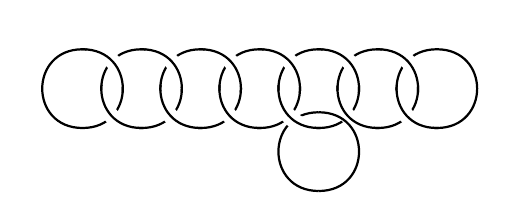
\begin{tikzpicture}
    \begin{knot}[clip width=7]
      \strand[thick] (0,0)
        to [out=left,in=left,looseness=1.75] (0,1)
        to [out=right,in=right,looseness=1.75] (0,0);
      \strand[thick] (0.75,0)
        to [out=left,in=left,looseness=1.75] (0.75,1)
        to [out=right,in=right,looseness=1.75] (0.75,0);
      \strand[thick] (1.5,0)
        to [out=left,in=left,looseness=1.75] (1.5,1)
        to [out=right,in=right,looseness=1.75] (1.5,0);
      \strand[thick] (2.25,0)
        to [out=left,in=left,looseness=1.75] (2.25,1)
        to [out=right,in=right,looseness=1.75] (2.25,0);
      \strand[thick] (3,0)
        to [out=left,in=left,looseness=1.75] (3,1)
        to [out=right,in=right,looseness=1.75] (3,0);
      \strand[thick] (3.75,0)
        to [out=left,in=left,looseness=1.75] (3.75,1)
        to [out=right,in=right,looseness=1.75] (3.75,0);
      \strand[thick] (4.5,0)
        to [out=left,in=left,looseness=1.75] (4.5,1)
        to [out=right,in=right,looseness=1.75] (4.5,0);
      \flipcrossings{1,3,5,7,9,11}
      \strand[thick] (3,-0.8)
        to [out=left,in=left,looseness=1.75] (3,0.2);
    \end{knot}
    \begin{knot}
      \strand[thick] (3,0.2)
        to [out=right,in=right,looseness=1.75] (3,-0.8);
    \end{knot}
  \end{tikzpicture}
\] Imagine this model as living in \(S^3\). Next, hollow out all these
rings: actually delete the portion of space that lies inside them! We
now have a 3-manifold \(M\) whose boundary \(\partial M\) consists of 8
connected components, each a torus. Of course, a solid torus also has a
torus as its boundary. So attach solid tori to each of these 8
components of \(\partial M\), but do it via this attaching map:
\[(x,y) \mapsto (y,-x+2y)\] where \(x\) and \(y\) are the obvious
coordinates on the torus, numbers between \(0\) and \(2\pi\), and we do
the arithmetic \(\mod 2\pi\). We now have a new 3-manifold without
boundary\ldots{} and this is the Poincare homology sphere.

We see here a strange and indirect connection between \(\mathrm{E}_8\)
and the dodecahedron. This is not the only such connection! There's also
the ``McKay correspondence'' (see \protect\hyperlink{week65}{``Week
65''}) and a way of getting the \(\mathrm{E}_8\) root lattice from the
``icosians'' (see \protect\hyperlink{week20}{``Week 20''}).

Are these three superficially different connections secretly just
different views of the same grand picture? I'm not sure. I think I'd
know the answer to part of this puzzle if I better understood the
relation between ADE theory and singularities.

But Diarmuid Crowley told me much more. The Poincare homology sphere is
actually the boundary of a 4-manifold, and it's not hard to say what
this 4-manifold is. I just gave you a recipe for cutting out 8 solid
tori from the 3-sphere and gluing them back in with a twist. Suppose we
think of 3-sphere as the boundary of the 4-disk \(D^4\), and think of
each solid torus as part of the boundary of a copy of
\(D^2 \times D^2\), using the fact that
\[\partial(D^2\times D^2) = S^1\times D^2 + D^2\times S^1.\] Then the
same recipe can be seen as instructions for gluing 8 copies of
\(D^2\times D^2\) to the 4-ball along part of their boundary, getting a
new 4-manifold with boundary. If you ponder it, you'll see that the
boundary of this 4-manifold is the Poincare homology 3-sphere.

Now, this is actually no big deal, at least for folks who know some
3-dimensional topology. But Crowley likes higher-dimensional topology,
and what he told me is this: the whole story generalizes to higher
dimensions! Instead of starting with this picture of linked 1-spheres in
the 3-sphere: \[
  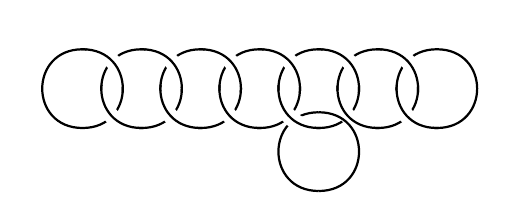
\begin{tikzpicture}
    \begin{knot}[clip width=7]
      \strand[thick] (0,0)
        to [out=left,in=left,looseness=1.75] (0,1)
        to [out=right,in=right,looseness=1.75] (0,0);
      \strand[thick] (0.75,0)
        to [out=left,in=left,looseness=1.75] (0.75,1)
        to [out=right,in=right,looseness=1.75] (0.75,0);
      \strand[thick] (1.5,0)
        to [out=left,in=left,looseness=1.75] (1.5,1)
        to [out=right,in=right,looseness=1.75] (1.5,0);
      \strand[thick] (2.25,0)
        to [out=left,in=left,looseness=1.75] (2.25,1)
        to [out=right,in=right,looseness=1.75] (2.25,0);
      \strand[thick] (3,0)
        to [out=left,in=left,looseness=1.75] (3,1)
        to [out=right,in=right,looseness=1.75] (3,0);
      \strand[thick] (3.75,0)
        to [out=left,in=left,looseness=1.75] (3.75,1)
        to [out=right,in=right,looseness=1.75] (3.75,0);
      \strand[thick] (4.5,0)
        to [out=left,in=left,looseness=1.75] (4.5,1)
        to [out=right,in=right,looseness=1.75] (4.5,0);
      \flipcrossings{1,3,5,7,9,11}
      \strand[thick] (3,-0.8)
        to [out=left,in=left,looseness=1.75] (3,0.2);
    \end{knot}
    \begin{knot}
      \strand[thick] (3,0.2)
        to [out=right,in=right,looseness=1.75] (3,-0.8);
    \end{knot}
  \end{tikzpicture}
\] start with an analogous pattern of 8 \(n\)-spheres linked in the
\((2n+1)\)-sphere. Do all the same stuff, boosting the dimensions
appropriately\ldots{} and you'll get an interesting (2n+1)-dimensional
manifold \(\partial M\) which is the boundary of a (2n+2)-dimensional
manifold M.

When n is \emph{odd} and greater than 1, this manifold \(\partial M\) is
actually an ``exotic sphere''. In other words, it's homeomorphic but not
diffeomorphic to the usual sphere of dimension 2n+1.

Now, exotic spheres of a given dimension form an abelian group G under
connected sum (see \protect\hyperlink{week141}{``Week 141''}). This
group consists of two parts: the easy part and the hard part. The easy
part is a normal subgroup \(N\) consisting of the exotic spheres that
bound parallelizable smooth manifolds. The size of this subgroup can be
computed in terms of Bernoulli numbers and stuff like that. The hard
part is the quotient group \(G/N\). This is usually the cokernel of a
famous gadget called the ``\(J\)-homomorphism''. I say ``usually''
because this is known to be true in most dimensions, but in certain
dimensions it remains an open question.

Anyway: the easy part \(N\) is always a finite cyclic group, and this is
\emph{generated} by the exotic sphere \(\partial M\) that I just
described!

For example:

In dimension 7 we have \(G = N = \mathbb{Z}/28\), so there are 28 exotic
spheres in this dimension (up to orientation-preserving diffeomorphism),
and they are all connected sums of the exotic 7-sphere \(\partial M\)
formed by the above construction.

In dimension 11 we have \(G = N = \mathbb{Z}/992\), so there are 992
exotic spheres, and they are all connected sums of the exotic 11-sphere
\(\partial M\) formed by the above construction.

In dimension 15 we no longer have \(G = N\). Instead we have
\(N = \mathbb{Z}/8128\) and \(G = \mathbb{Z}/8128\oplus \mathbb{Z}/2\).
There are thus 16256 exotic spheres in this dimension, only half of
which are connected sums of the exotic 15-sphere \(\partial M\) formed
by the above construction.

And so on.

While we're on the subject of exotic 15-spheres, I can't resist
mentioning this. I explained in \protect\hyperlink{week141}{``Week
141''} how to construct a bunch of exotic 7-spheres (24 of them,
actually) using the quaternions. Once you understand this trick, it's
natural to wonder if you can construct exotic 15-spheres the same way,
but using octonions instead of quaternions. Well, you can:

\begin{enumerate}
\def\labelenumi{\arabic{enumi})}
\setcounter{enumi}{2}
\tightlist
\item
  Nobuo Shimada, ``Differentiable structures on the 15-sphere and
  Pontrjagin classes of certain manifolds'', \emph{Nagoya Math. Jour.}
  \textbf{12} 1957, 59--69.
\end{enumerate}

I should also explain what I really like about the above stuff. In
topological quantum field theory, people like to get 3-manifolds by
``surgery on framed links''. The idea is to start with a framed link in
the 3-sphere, use the framing to thicken each component to an embedded
solid torus, cut out these solid tori, and reattach them ``the other
way'', using the fact that \(S^1\times S^1\) is the boundary of both
\(S^1\times D^2\) and \(D^2\times S^1\). We can get any compact oriented
3-manifold this way.

The above construction of the Poincare homology sphere was just an
example of this, where the link was \[
  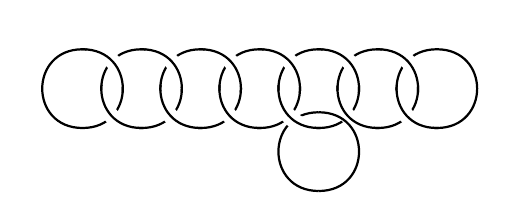
\begin{tikzpicture}
    \begin{knot}[clip width=7]
      \strand[thick] (0,0)
        to [out=left,in=left,looseness=1.75] (0,1)
        to [out=right,in=right,looseness=1.75] (0,0);
      \strand[thick] (0.75,0)
        to [out=left,in=left,looseness=1.75] (0.75,1)
        to [out=right,in=right,looseness=1.75] (0.75,0);
      \strand[thick] (1.5,0)
        to [out=left,in=left,looseness=1.75] (1.5,1)
        to [out=right,in=right,looseness=1.75] (1.5,0);
      \strand[thick] (2.25,0)
        to [out=left,in=left,looseness=1.75] (2.25,1)
        to [out=right,in=right,looseness=1.75] (2.25,0);
      \strand[thick] (3,0)
        to [out=left,in=left,looseness=1.75] (3,1)
        to [out=right,in=right,looseness=1.75] (3,0);
      \strand[thick] (3.75,0)
        to [out=left,in=left,looseness=1.75] (3.75,1)
        to [out=right,in=right,looseness=1.75] (3.75,0);
      \strand[thick] (4.5,0)
        to [out=left,in=left,looseness=1.75] (4.5,1)
        to [out=right,in=right,looseness=1.75] (4.5,0);
      \flipcrossings{1,3,5,7,9,11}
      \strand[thick] (3,-0.8)
        to [out=left,in=left,looseness=1.75] (3,0.2);
    \end{knot}
    \begin{knot}
      \strand[thick] (3,0.2)
        to [out=right,in=right,looseness=1.75] (3,-0.8);
    \end{knot}
  \end{tikzpicture}
\] and each component had two twists in the framing as we go around, as
compared to the standard ``blackboard'' framing. This is why there was
that mysterious number ``2'' in my formula for the attaching map.

Whenever we describe a 3-manifold using ``surgery on framed links'' this
way, there's an important matrix where the entry in the \(i\)th row and
\(j\)th column is the linking number of the \(i\)th component and the
\(j\)th component of our framed link, with the diagonal entries standing
for the ``self-linking'' numbers of the components, that is, the number
of twists their framings have. This matrix is important because it also
describes the ``intersection form'' on the 2nd homology group of a
simply-connected 4-manifold \(M\) whose boundary \(\partial M\) is the
3-manifold we're describing.

For example, in the case of the Poincare homology sphere, this matrix is
called the \(\mathrm{E}_8\) Cartan matrix: \[
  \left(
    \begin{array}{rrrrrrrr}
      2&-1&0&0&0&0&0&0
    \\-1&2&-1&0&0&0&0&0 
    \\0&-1&2&-1&0&0&0&0 
    \\0&0&-1&2&-1&0&0&0 
    \\0&0&0&-1&2&-1&0&-1
    \\0&0&0&0&-1&2&-1&0
    \\0&0&0&0&0&-1&2&0 
    \\0&0&0&0&-1&0&0&2
    \end{array}
  \right)
\] The Dynkin diagram simply summarizes this matrix in pictorial form. I
already described the 4-manifold \(M\) whose boundary is the Poincare
homology sphere; now you know its intersection form.

Anyway, what I find exciting is that all this stuff generalizes to
higher dimensions if we restrict attention to manifolds that have
trivial homotopy groups up to a certain point! For example, it works for
compact oriented smooth 7-manifolds that have trivial \(\pi_1\) and
\(\pi_2\). Any such manifold can be obtained by doing surgery on some
framed 3-spheres embedded in \(S^7\). Just as 1-spheres can link in 3d
space since 1+1 is one less than 3, 3-spheres can link in 7d space since
3+3 is one less than 7. We again get a matrix of linking numbers. As
before, this matrix is also an intersection form: namely, the
intersection form on the 4th homology group of an 8-manifold M whose
boundary \(\partial M\) is the 7-manifold we're describing. Moreover,
this matrix is symmetric in both the 3-manifold example and the
7-manifold example, since it describes an intersection pairing on an
\emph{even-dimensional} homology group.

Even better, all the same stuff happens in manifolds with enough trivial
homotopy groups in dimension 11, and dimension 15\ldots{} and all
dimensions of the form \(4n-1\). And what's \emph{really} neat is that
these higher-dimensional generalizations are in some ways simpler than
the 3d story. The reason is that a 1-sphere can be knotted in 3-space in
really complicated ways, but the higher-dimensional generalizations do
not involve such complicated knotting. The framing aspects can be more
complicated, since there's more to framing an embedded sphere than just
an integer, but it's not all \emph{that} complicated.

So maybe I can learn some more 3d topology by first warming up with the
simpler 7d case\ldots.

Finally, I'd like to list a few articles that I've been meaning to read,
but haven't gotten around to. I hope to read them sometime \emph{this}
millennium! I'll quote the abstracts and make a few comments.

\begin{enumerate}
\def\labelenumi{\arabic{enumi})}
\setcounter{enumi}{3}
\tightlist
\item
  Jack Morava, ``Cobordism of symplectic manifolds and asymptotic
  expansions'', a talk at the conference in honor of S.P. Novikov's 60th
  birthday, available as
  \href{https://arxiv.org/abs/math.SG/9908070}{\texttt{math.SG/9908070}}.
\end{enumerate}

\begin{quote}
The cobordism ring of symplectic manifolds defined by V.L. Ginzburg is
shown to be isomorphic to the Pontrjagin ring of complex-oriented
manifolds with free circle actions. This suggests an interpretation of
the formal group law of complex cobordism, in terms of a composition-law
on semiclassical expansions. An appendix discusses related questions
about cobordism of toric varieties.
\end{quote}

I started trying to explain the relation between formal group laws and
complex oriented cohomology theories in
\protect\hyperlink{week150}{``Week 150''}, because I'm quite puzzled
about the deep inner meaning of this relation. This paper might be the
key to this mystery!

\begin{enumerate}
\def\labelenumi{\arabic{enumi})}
\setcounter{enumi}{4}
\tightlist
\item
  Detlev Buchholz, ``Current trends in axiomatic quantum field theory'',
  available as
  \href{https://arxiv.org/abs/hep-th/9811233}{\texttt{hep-th/9811233}}.
\end{enumerate}

\begin{quote}
In this article a non-technical survey is given of the present status of
Axiomatic Quantum Field Theory and interesting future directions of this
approach are outlined. The topics covered are the universal structure of
the local algebras of observables, their relation to the underlying
fields and the significance of their relative positions. Moreover, the
physical interpretation of the theory is discussed with emphasis on
problems appearing in gauge theories, such as the revision of the
particle concept, the determination of symmetries and statistics from
the superselection structure, the analysis of the short distance
properties and the specific features of relativistic thermal states.
Some problems appearing in quantum field theory on curved spacetimes are
also briefly mentioned.
\end{quote}

I've been falling behind on new developments in axiomatic quantum field
theory. Lots of cool stuff is happening, I hear. This might help me
catch up.

\begin{enumerate}
\def\labelenumi{\arabic{enumi})}
\setcounter{enumi}{5}
\tightlist
\item
  Matt Visser, ``The reliability horizon'', available as
  \href{https://arxiv.org/abs/gr-qc/9710020}{\texttt{gr-qc/9710020}}.
\end{enumerate}

\begin{quote}
The ``reliability horizon'' for semi-classical quantum gravity
quantifies the extent to which we should trust semi-classical quantum
gravity, and gives a handle on just where the ``Planck regime'' resides.
The key obstruction to pushing semi-classical quantum gravity into the
Planck regime is often the existence of large metric fluctuations,
rather than a large back-reaction.
\end{quote}

This seems like a very sensible enterprise: determining just where
semiclassical calculations are likely to break down, and quantum gravity
effects to become important. Why haven't I read this? It's obviously
worthwhile!

\begin{enumerate}
\def\labelenumi{\arabic{enumi})}
\setcounter{enumi}{6}
\tightlist
\item
  Bianca Letizia Cerchiai and Julius Wess, ``\(q\)-Deformed Minkowski
  Space based on a \(q\)-Lorentz Algebra'', available as
  \href{https://arxiv.org/abs/math.QA/9801104}{\texttt{math.QA/9801104}}.
\end{enumerate}

\begin{quote}
The Hilbert space representations of a non-commutative \(q\)-deformed
Minkowski space, its momenta and its Lorentz boosts are constructed. The
spectrum of the diagonalizable space elements shows a lattice-like
structure with accumulation points on the light-cone.
\end{quote}

The \(q\)-deformed Lorentz algebra plays a role in quantum gravity with
nonzero cosmological constant, but it also shows up in noncommutative
geometry. Are the two roles related? I don't know! This is on my list of
puzzles to ponder.

The people applying the \(q\)-deformed Lorentz algebra to noncommutative
geometry want to develop the theory of \(q\)-deformed Minkowski space,
see if it makes the infinities in quantum field theory go away, and see
what physical predictions it makes. It makes spacetime discrete in a
very pretty way; that I know from Julius Wess' talk in Schladming a few
years back (see \protect\hyperlink{week129}{``Week 129''}). But I should
learn more about this, and not just because Bianca Letizia Cerchiai is a
very nice person who invited my girlfriend and I to lunch at her
parents' apartment in Milan\ldots. oh, now I'm feeling \emph{terribly}
guilty for not reading her paper! How nasty of me! I'd better print it
out and read it as soon as I go into the office!

In fact, now that I think of it, I've had at least \emph{some} dealings
with \emph{all} the authors of these papers. And now I'm publicly
admitting I haven't read some of their most interesting papers! Ugh! At
least this admission may shame me into reading them now\ldots{}

Bye.

\begin{center}\rule{0.5\linewidth}{0.5pt}\end{center}

On \texttt{sci.physics.research}, Aaron Bergman clarified something
about these millennial physics problems:

\begin{quote}
John Baez wrote:

\begin{quote}
Aaron Bergman (\texttt{abergman@Princeton.EDU}) wrote:

\begin{quote}
John Baez wrote:

\begin{quote}
Of course, this business of limiting ``physics'' to mean ``the search
for fundamental laws'' annoys condensed matter physicists like Philipp
Anderson, since it excludes everything they work on.
\end{quote}

One should note that Gross explicitly says --- there's a Realaudio of
the talk online --- that this is a very narrowminded list that excludes
fundamental questions in other fields. It's not really intended to be a
universal list.
\end{quote}

Good! It's too bad the text of the webpage doesn't make that clearer.
I'm appending your comment to the version of
\protect\hyperlink{week164}{``Week 164''} on my website, assuming you
don't object.
\end{quote}

Sure. Or you can just refer them to the transparencies and the talk. For
those who don't want to bother listening to the whole thing, start
listening at about 7:30 mins into the RealAudio stream:

\texttt{http://feynman.physics.lsa.umich.edu/cgi-bin/s2ktalk.cgi?questions}

It's on transparency 4 which is why I mentioned,

\begin{quote}
\begin{quote}
And Witten is coming back.
\end{quote}

You mean he's not staying in LA? Can't take the winters out here?
\end{quote}

I won't speculate on the reasons, but his grad students have said that
he's coming back to the Institute.

Aaron

--- Aaron Bergman
\end{quote}



\hypertarget{week165}{%
\section{March 14, 2001}\label{week165}}

A few weeks ago I went to the University of Wisconsin at Milwaukee to
give some talks at their Center for Gravitation and Cosmology. They have
a group of 8 people working on data analysis for the LIGO experiment. As
you probably know, LIGO will use laser interferometry to look for
gravitational waves. It consists of two detectors, one near Livingston,
Louisiana, and one near Hanford, Washington. Each one is shaped like an
L, with each arm of the L consisting of a 4-kilometer-long evacuated
pipe with a laser beam running down it. A typical gravitational wave
might stretch one of the arms by \(10^{-16}\) centimeters --- one
hundred-millionth of the diameter of a hydrogen atom. It will be quite
exciting if they can actually get this level of precision. They're not
there yet, but already they can tell when wind-blown tumbleweeds pile up
along the pipe at the Hanford site, because their gravitational pull
bends the beam and messes things up!

In Milwaukee, it's a time of preparation and anticipation. The first
data should start coming in by September, but right now they're busy
writing software and assembling a ``Beowulf cluster''. This is a
parallel computer formed from a bunch of commercially available
processors, all running Linux. I'd heard about these before, because my
friend Dan Christensen is planning to do calculations in spin foam
models of quantum gravity on a Beowulf cluster over at the University of
Western Ontario. The cluster at Milwaukee will have 128 processors, each
with at least 1 gigaflop peak performance, and a total of 19 terabytes
of distributed disk memory.

You can learn more about this at their homepage:

\begin{enumerate}
\def\labelenumi{\arabic{enumi})}
\tightlist
\item
  University of Wisconsin at Milwaukee, Center for Gravitation and
  Cosmology home page, \texttt{http://www.gravity.phys.uwm.edu/}
\end{enumerate}

For a nice popular account of the LIGO experiment, try this:

\begin{enumerate}
\def\labelenumi{\arabic{enumi})}
\setcounter{enumi}{1}
\tightlist
\item
  Marcia Bartusiak, \emph{Einstein's Unfinished Symphony: Listening to
  the Sounds of Space-Time}, Joseph Henry Press, Washington D.C., 2000.
\end{enumerate}

My host was at Milwaukee was John Friedman. I was surprised and pleased
to find that he was one of the people who discovered how to make
spin-\(1/2\) particles out of topological defects in spacetime!
Theoretically speaking, that is. I'd heard about this trick, but I never
knew where it came from:

\begin{enumerate}
\def\labelenumi{\arabic{enumi})}
\setcounter{enumi}{2}
\tightlist
\item
  J. Friedman and R. Sorkin, ``Spin \(1/2\) from gravity'', \emph{Phys.
  Rev.~Lett.} \textbf{44} (1980), 1100.
\end{enumerate}

I was more familiar with a recent implementation of it in the framework
of loop quantum gravity, as mentioned in
\protect\hyperlink{week128}{``Week 128''}.

Friedman and Sorkin's trick was based on the idea of ``dyons''. I'd
never understood dyons, but Friedman explained them to me, and now the
idea seems so simple that I can't resist telling everyone.

To make a ``dyon'', just take a charged particle and a magnetic monopole
and tape them together with high-quality duct tape. You can buy all
these materials at your local hardware store\ldots{} though mine was out
of monopoles when I last checked.

Now, rotate your dyon. As you move the charged particle around the
monopole, it picks up a phase, thanks to the magnetic field.
Alternatively, as you move the monopole around charged particle, it
picks up a phase thanks to the electric field! Either way, you get the
same phase when you move one of these guys all the way around the other
--- and this phase has to be \(1\) or \(-1\) for well-known topological
reasons. If the phase is \(1\), your dyon is a boson. But if the phase
is \(-1\), your dyon is a fermion!

In short, this is a strange and interesting way to build fermions out of
components that are not themselves fermionic.

In Milwaukee, I gave a talk where I tried to explain the meaning of
Einstein's equation in simple English. There are a lot of books that
give simple explanations of curved spacetime, geodesics and so on.
Unfortunately, most of them don't explain the real meat of general
relativity: Einstein's equation. This bugs me, especially since it's not
so hard. If you're interested, take a look at this:

\begin{enumerate}
\def\labelenumi{\arabic{enumi})}
\setcounter{enumi}{3}
\tightlist
\item
  John Baez, ``The meaning of Einstein's equation'', available at
  \href{https://arxiv.org/abs/gr-qc/0103044}{\texttt{gr-qc/0103044}}.
\end{enumerate}

Since my Milwaukee trip I've become really busy writing notes on the
quantum gravity seminar here at Riverside. Toby Bartels and I have been
writing them up in the form of a rather silly dialog, and my student
Miguel Carrion-Alvarez has been been writing them in a more traditional
format. Eventually they will be put together in the form of a book, but
it's a lot of work. That's the main reason This Week's Finds has been
dormant lately. You can see all these notes here:

\begin{enumerate}
\def\labelenumi{\arabic{enumi})}
\setcounter{enumi}{4}
\tightlist
\item
  John Baez, Toby Bartels and Miguel Carrion, \emph{Quantum Gravity
  Seminar}, \texttt{http://math.ucr.edu/home/baez/qg.html}
\end{enumerate}

The ultimate goal is to describe spin foam models of 4d quantum gravity,
but we're only gradually working our way to that point.

There are a lot of other things I'd like to talk about, but I don't have
time to do them all justice. For example, there's a nice new book of
essays on quantum gravity:

\begin{enumerate}
\def\labelenumi{\arabic{enumi})}
\setcounter{enumi}{5}
\tightlist
\item
  Craig Callender and Nick Huggett, eds., \emph{Physics Meets Philosophy
  at the Planck Scale: Contemporary Theories in Quantum Gravity},
  Cambridge U. Press, Cambridge, 2001.
\end{enumerate}

It has articles by Chris Isham, Carlo Rovelli, Ed Witten and other
folks. I found Gordon Belot and John Earman's ``Pre-Socratic Quantum
Gravity'' to be a particularly clear-headed account of the so-called
``problem of time'' in quantum gravity. I wish it had existed when I was
first struggling to understand this subject! Everyone trying to
understand quantum gravity should read this.

Over on the more technical end, Martin Bojowald has written a bunch of
papers applying loop quantum gravity to the big bang, which I want to
catch up with:

\begin{enumerate}
\def\labelenumi{\arabic{enumi})}
\setcounter{enumi}{6}
\item
  Martin Bojowald, ``Loop Quantum Cosmology I: Kinematics'',
  \emph{Class. Quant. Grav.} \textbf{17} (2000), 1489--1508, also
  available at
  \href{https://arxiv.org/abs/gr-qc/9919103}{\texttt{gr-qc/9919103}}

  ``Loop Quantum Cosmology II: Volume Operators'', \emph{Class. Quant.
  Grav.} \textbf{17} (2000), 1509--1526, also available at
  \href{https://arxiv.org/abs/gr-qc/9910104}{\texttt{gr-qc/9910104}}.

  ``Loop Quantum Cosmology III: Wheeler-DeWitt Operators'', \emph{Class.
  Quant. Grav.} \textbf{18} (2001), 1055--1070, also available at
  \href{https://arxiv.org/abs/gr-qc/0008052}{\texttt{gr-qc/0008052}}.

  ``Loop Quantum Cosmology IV: Discrete Time Evolution'', \emph{Class.
  Quant. Grav.} \textbf{18} (2001) 1071--1088, also available at
  \href{https://arxiv.org/abs/gr-qc/0008053}{\texttt{gr-qc/0008053}}.

  ``Absence of Singularity in Loop Quantum Cosmology'', available at
  \href{https://arxiv.org/abs/gr-qc/0102069}{\texttt{gr-qc/0102069}}.
\end{enumerate}

The really interesting ones are the last two, whose titles explain why
they're interesting --- but they're based on the framework developed in
the earlier papers.

And then there's \(n\)-category theory! Two of Martin Hyland's students
have been making interesting progress on this subject. Tom Leinster has
been studying operads, their generalizations, their relation to homotopy
theory, and their application to \(n\)-categories. He's even given a new
definition of ``weak \(n\)-category'', thus adding to the profusion of
competing candidates:

\begin{enumerate}
\def\labelenumi{\arabic{enumi})}
\setcounter{enumi}{7}
\item
  Tom Leinster, ``General operads and multicategories'', available as
  \href{https://arxiv.org/abs/math.CT/9810053}{\texttt{math.CT/9810053}}.

  \emph{Structures in higher-dimensional category theory}, Ph.D.~thesis,
  available at
  \texttt{http://www.dpmms.cam.ac.uk/\textasciitilde{}leinster/shdctabs.html}

  ``Up-to-homotopy monoids'', available as
  \href{https://arxiv.org/abs/math.QA/9912084}{\texttt{math.QA/9912084}}.

  ``Homotopy algebras for operads'', available as
  \href{https://arxiv.org/abs/math.QA/0002180}{\texttt{math.QA/0002180}}.

  ``Operads in higher-dimensional category theory'', available as
  \href{https://arxiv.org/abs/math.CT/0011106}{\texttt{math.CT/0011106}}
\end{enumerate}

Eugenia Cheng, on the other hand, seems to be working to \emph{reduce}
the number of different definitions of weak \(n\)-category, by laying
the groundwork for connecting various existing definitions --- mainly
those based on ``opetopes'' and related shapes:

\begin{enumerate}
\def\labelenumi{\arabic{enumi})}
\setcounter{enumi}{8}
\item
  Eugenia Cheng, ``The relationship between the opetopic and multitopic
  approaches to weak \(n\)-categories'', available at
  \texttt{http://www.dpmms.cam.ac.uk/\textasciitilde{}elgc2/}

  ``Equivalence between approaches to the theory of opetopes'',
  available at
  \texttt{http://www.dpmms.cam.ac.uk/\textasciitilde{}elgc2/}
\end{enumerate}

I'm glad these energetic young folks are stepping in to help out the
older folks like me who have become completely exhausted from thinking
about \(n\)-categories.

Finally, everyone who wants to understand M-theory and its relation to
matrix models should first read this review article by Nicolai and
Helling:

\begin{enumerate}
\def\labelenumi{\arabic{enumi})}
\setcounter{enumi}{9}
\tightlist
\item
  Hermann Nicolai and Robert Helling, ``Supermembranes and M(atrix)
  theory'', available as
  \href{https://arxiv.org/abs/hep-th/9809103}{\texttt{hep-th/9809103}}.
\end{enumerate}

and then this new review article by Wati Taylor:

\begin{enumerate}
\def\labelenumi{\arabic{enumi})}
\setcounter{enumi}{9}
\tightlist
\item
  Washington Taylor, ``M(atrix) theory: matrix quantum mechanics as a
  fundamental theory'', available as
  \href{https://arxiv.org/abs/hep-th/0101126}{\texttt{hep-th/0101126}}.
\end{enumerate}

They're both pretty cool. How does a theory of matrices wind up acting
like a theory of membranes? That's what you'll understand if you study
this stuff.



\hypertarget{week166}{%
\section{March 27, 2001}\label{week166}}

Do you know this number?
\[2.685452001065306445309714835481795693820382293994462953051152\ldots\]
They say that mathematics is not really about numbers, and they're
right. But sometimes it's fun to play around with the darn things!

Given any positive number you can work out its continued fraction
expansion, like this:
\[\sqrt{2} = 1+\frac{1}{2+\frac{1}{2+\frac{1}{2+_{\ldots}}}}\] But
normally it won't look so pretty! A number is rational if and only if
the continued fraction stops after finitely many steps. If its continued
fraction expansion eventually repeats, like this:
\[\sqrt{3} = 1+\frac{1}{1+\frac{1}{2+\frac{1}{1+_{\ldots}}}}\] then it
satisfies a quadratic equation with integer coefficients. So the
continued fraction expansion of e can't ever repeat\ldots{} but it's
cute nonetheless:
\[e = 2+\frac{1}{1+\frac{1}{2+\frac{1}{1+\frac{1}{1+\frac{1}{4+\frac{1}{1+\frac{1}{1+\frac{1}{6+_{\ldots}}}}}}}}}\]
It continues on predictably after that initial hiccup. The number
\(\pi\), on the other hand, gives a random-looking mess. This is a hint
that \(\pi\) is number-theoretically more complicated than \(e\), which
is also apparent when you compare the proofs that \(e\) and \(\pi\) are
transcendental --- the proof for \(e\) is much easier.

Pondering all this, it's natural to ask about the ``average'' behavior
of the continued fraction expansion of a number. What's the average
behavior of the series \(a_1, a_2, a_3, \ldots\) that we get this way:
\[x=a_1+\frac{1}{a_2+\frac{1}{a_3+\frac{1}{a_4+_{\ldots}}}}\] It turns
out that if we take the geometric mean of the first \(n\) terms and then
let \(n\) approach \(\infty\), the mean almost always converges to
``Khinchin's constant'' --- the number at the beginning of this article!
Here by ``almost always'' I mean that the set of exceptions has measure
zero. One can prove this using some ideas from ergodic theory.

Now, there is much more to say about continued fraction expansions, but
my real goal is simply to point out that there are lots of interesting
constants in mathematics besides \(\pi\), \(e\), the golden ratio, and
Euler's number. Where can you read about them? Here:

\begin{enumerate}
\def\labelenumi{\arabic{enumi})}
\tightlist
\item
  Steven Finch, ``MathSoft Constants'',
  \texttt{http://pauillac.inria.fr/algo/bsolve/constant/constant.html}
\end{enumerate}

This is a great place to learn about Khinchin's constant, Feigenbaum's
number, Madelung's constant, Artin's constant, Grothendieck's constant,
and many other fun numbers!

Speaking of fun websites, here's another:

\begin{enumerate}
\def\labelenumi{\arabic{enumi})}
\setcounter{enumi}{1}
\tightlist
\item
  The Mathematics Genealogy Project,
  \texttt{http://hcoonce.math.mankato.msus.edu/}
\end{enumerate}

My advisor's advisor's advisor's advisor's advisor's advisor's advisor's
advisor was Gauss. If you think I'm showing off, you're right! But I
couldn't have done it without this website, and if you're a
mathematician, there's a good chance you use it to track down
\emph{your} academic lineage. And if you can't, you can at least add
your information to the database.

Before Demian Cho showed me this site, I'd gotten stuck 3 generations
back in my attempts to discover my academic ancestors. Now I can go back
11 generations. I know it's annoying, but I'm gonna tell you the whole
story:

My advisor was Irving Segal, the guy who helped prove the
Gelfand-Naimark-Segal theorem. This is a basic result about
\(C^*\)-algebras, a kind of gadget he invented to formalize the notion
of an ``algebra of observables'' in quantum theory. The GNS theorem
implies that every \(C^*\)-algebra sits inside the algebra of all
bounded operators on some Hilbert space, so it's a kind of justification
for using Hilbert spaces in quantum physics. But even better, it gives a
procedure for representing a \(C^*\)-algebra as operators on a Hilbert
space starting from a ``state'' on the \(C^*\)-algebra. The upshot is
that while Hilbert spaces are important, the right Hilbert space to use
can depend on the state of the system you're studying. At first people
thought Segal was nuts for saying this, but by now it's well-accepted.

Segal also did work on quantum field theory, nonlinear partial
differential equations, and other topics at the borderline between
physics and functional analysis. His students include Isadore Singer and
Bertram Kostant, whose work on geometric quantization generalized
Segal's ideas on the ``Bargmann-Segal representation''. I worked with
Segal because I liked analysis and wanted to understand quantum field
theory in a rigorous way.

Segal's advisor was Einar Hille, the guy who helped prove the
Hille-Yosida theorem. Hille did a lot of work on integral and
differential equations, but later he became interested in functional
analysis: the study of infinite-dimensional vector spaces equipped with
nice topologies, such as Hilbert spaces, Banach spaces and the like. At
the time, he was rather special in his emphasis on applying these
abstract ideas to concrete problems. In his book ``Methods in Classical
and Functional Analysis,'' he wrote:

\begin{quote}
If the book has a thesis, it is that a functional analyst is an analyst,
first and foremost, and not a degenerate species of a topologist. His
problems come from analysis and his results should throw light on
analysis\ldots.
\end{quote}

The Hille-Yosida theorem shows how to write a large class of
one-parameter semigroups of linear operators on Banach spaces in the
form \(\exp(-tH)\). These so-called ``contraction semigroups'' naturally
come from the heat equation and its relatives. Segal was fond of this
idea, and he generalized it to semigroups of nonlinear operators, which
arise naturally from \emph{nonlinear} partial differential equations. He
used this idea to prove global existence of solutions for various
nonlinear classical field theories.

Hille's advisor was Marcel Riesz, the guy who didn't prove the Riesz
representation theorem. Marcel's brother Frigyes was the guy who did
that. Marcel worked on functional analysis, partial differential
equations, and mathematical physics --- even Clifford algebras and
spinors!

The advisor of Marcel Riesz was Lipot Fejer, the guy who discovered the
Fejer kernel. This shows up when you sum Fourier series. If you just
naively sum the Fourier series of a continuous function on the circle,
it may not converge uniformly. However, if you use a trick called Cesaro
summation, which amounts to averaging the partial sums, you get uniform
convergence. The average of the first \(n\) partial sums of the Fourier
series of your function is equal to its convolution with the Fejer
kernel. Fejer also worked on conformal mappings. His students included
Paul Erdos and Gabor Szego.

Fejer's advisor was Karl Herman Amandus Schwarz, the guy who helped
prove the Cauchy-Schwarz inequality. That's a wonderful inequality which
everyone should know! But Schwarz also worked on minimal surfaces and
complex analysis: for example, conformal mappings from polyhedra into
the sphere, and also the Dirichlet problem. Don't mix him up with
Laurent Schwartz, the guy who invented distributions.

(Actually, Lipot Fejer's name was originally Leopold Weiss. He changed
it to seem more Hungarian. This was a common practice at the time in
Hungary, but when he did it, his advisor Schwarz stopped speaking to
him!)

Schwarz's advisor was Karl Weierstrass, the guy who proved the
Weierstrass theorem. This theorem says that every continuous real-valued
function on the unit interval is a uniform limit of polynomials.
Weierstrass also has a function named after him: the Weierstrass
elliptic function, which I explained in
\protect\hyperlink{week13}{``Week 13''}. But his real claim to fame is
how he made analysis more rigorous! For example, he discovered the
importance of uniform convergence, and found a continuous function with
no derivative at any point. Besides Schwarz, his students include
Frobenius, Killing, and Kowalevsky.

Now, Weierstrass doesn't have an advisor listed in the mathematics
genealogy. However, by using this website full of mathematician's
biographies, I can go back further:

\begin{enumerate}
\def\labelenumi{\arabic{enumi})}
\setcounter{enumi}{2}
\tightlist
\item
  John J. O'Connor and Edmund F. Robertson, ``The MacTutor History of
  Mathematics Archive'',
  \texttt{http://www-groups.dcs.st-andrews.ac.uk/\textasciitilde{}history/index.html}
\end{enumerate}

According to this, Weierstrass had an erratic career as a student: his
father tried to make him study finance instead of math, so he spent his
undergraduate years fencing and drinking. He learned a lot of math on
his own, and got really interested in elliptic functions from the work
of Abel and Jacobi. I can't tell if he ever had an official dissertation
advisor. However, in 1839 he went to the Academy at Muenster to study
under Christoph Gudermann, who worked on elliptic functions and
spherical geometry. Gudermann strongly encouraged Weierstrass in his
mathematical studies. Weierstrass asked for a question on elliptic
functions, and wound up writing a paper which Gudermann assessed
``\ldots{} of equal rank with the discoverers who were crowned with
glory.'' (When Weierstrass heard this, he commended Gudermann's
generosity, since he had strongly criticized Gudermann's methods.)

Given all this, and the fact that Weierstrass seems to have had no
\emph{other} mentor, I'll declare Gudermann to be his advisor, de facto
even if not officially.

But who was Gudermann? He's the guy they named the ``gudermannian''
after! That's this function:
\[\mathrm{gd}(u) = 2 \arctan(\exp(u)) - \frac\pi2.\] Now, if you're
wondering why such a silly function deserves a name, you should work out
its inverse function: \[\mathrm{gd}^{-1}(x) = \ln(\sec(x) + \tan(x)).\]
And if you don't recognize \emph{this}, you probably haven't taught
freshman calculus lately! It's the integral of \(\sec(x)\), which is one
of the hardest of the basic integrals you teach in that kind of course.
But it's not just hard, it's historically important: a point at latitude
\(\mathrm{gd}(u)\) has distance \(u\) from the equator in a Mercator
projection map. If you think about it a while, this is precisely what's
needed to make the projection be a conformal transformation --- that is,
angle-preserving. And that's just what you want if you're sailing a ship
in a constant direction according to a compass and you want to know
where you'll wind up.

If you don't see how this works, try:

\begin{enumerate}
\def\labelenumi{\arabic{enumi})}
\setcounter{enumi}{3}
\tightlist
\item
  Wikipedia, \texttt{http://en.wikipedia.org/wiki/Mercator\_projection}
\end{enumerate}

Gudermann's advisor was Carl Friedrich Gauss, the guy they named
practically \emph{everything} after! Poor Gudermann, who was content to
mess around with special functions and spherical geometry, seems to have
been one of Gauss' worst students. But that's not so bad, since three of
the other four were Bessel, Dedekind and Riemann.

Gauss' advisor was Johann Pfaff, the guy they named the ``Pfaffian''
after. If the matrix A is skew-symmetric, we can write
\[\det(A) = \operatorname{Pf}(A)^2\] where \(\operatorname{Pf}(A)\) is
also a polynomial in the entries of \(A\). Pfaffians now show up in the
study of fermionic wavefunctions. Pfaff worked on various things,
including the integrability of partial differential equations, where the
concept of a ``Pfaffian system'' is important. Unfortunately I've never
gotten around to understanding these.

Pfaff's advisor was Abraham Kaestner. I'd never heard of him before now.
He wrote a 4-volume history of mathematics, but his most important work
was on axiomatic geometry. His interest in the parallel postulate
indirectly got Gauss, Bolyai and Lobachevsky interested in that topic:
we've already seen that he taught Gauss' advisor, but he also taught
Bolyai's father, as well as Lobachevsky's teacher, one J. M. C. Bartels.
In fact, Kaestner was still teaching when Gauss went to school, but
Gauss didn't go to Kaestner's courses, because he found them too
elementary. Gauss said of him, ``He is the best poet among
mathematicians and the best mathematician among poets''. Perhaps this
faint praise refers to Kaestner's knack for aphorisms.

At this point I got stuck until my student Miguel Carrion-Alvarez helped
out. It appears that Kaestner's advisor was one Christian A. Hausen.
He's the guy they named the Hausen crater after --- a lunar crater
located at 65.5 S, 88.4 W. He did his thesis on theology in 1713, but
became a professor of mathematics in Leipzig. He worked on
electrostatics, but made no memorable discoveries.

At this point the trail disappears into mist. For some conjectures, see
this page:

\begin{enumerate}
\def\labelenumi{\arabic{enumi})}
\setcounter{enumi}{4}
\tightlist
\item
  Anthony M. Jacobi, ``Academic Family Tree'',
  \texttt{http://www.staff.uiuc.edu/\%7Ea-jacobi/tree.html}
\end{enumerate}

It's interesting how the same themes keep popping up in this genealogy.
For example, Weierstrass invented uniform convergence and proved that
the limit of a uniformly convergent series of continuous functions is
continuous. The Fejer kernel shows up when you're trying to write
functions on the circle as a uniformly convergent sum of complex
exponentials. Segal's \(C^*\)-algebras generalize the notion of uniform
convergence to operator algebras. I guess these things just go from
generation to generation\ldots.

A little while ago John McKay visited me and told me about all sorts of
wonderful things: relations between subgroups of the Monster group,
exceptional Lie groups, and modular forms\ldots{} a presentation of the
Monster group with 2 generators, a way to build the Leech lattice from 3
copies of the \(\mathrm{E}_8\) lattice\ldots{} a way to get ahold of the
Monster group starting with a diagram with 26 nodes\ldots.

Unfortunately, I'm having trouble finding references for some of these
things! It's possible that the last two items are really these:

\begin{enumerate}
\def\labelenumi{\arabic{enumi})}
\setcounter{enumi}{5}
\item
  Robert L. Griess, ``Pieces of eight: semiselfdual lattices and a new
  foundation for the theory of Conway and Mathieu groups''. \emph{Adv.
  Math.} \textbf{148} (1999), 75--104.
\item
  John H. Conway, Christopher S. Simons, ``26 implies the Bimonster'',
  \emph{Jour. Algebra} \textbf{235} (2001), 805--814.
\end{enumerate}

Anyway, I need to read about this stuff.

Speaking of exceptionology: in \protect\hyperlink{week163}{``Week 163''}
I explained how \(\mathrm{Spin}(9)\) sits inside the Lie group
\(\mathrm{F}_4\), thanks to the fact that \(\mathrm{Spin}(9)\) is the
automorphism group of Jordan algebra of \(2\times2\) hermitian
octonionic matrices, and \(\mathrm{F}_4\) is the automorphism group of
the Jordan algebra of \(3\times\) hermitian matrices. But in fact, since
there are different ways to think of \(2\times2\) matrices as special
\(3\times\) matrices, there are actually 3 equally good ways to stuff
\(\mathrm{Spin}(9)\) in \(\mathrm{F}_4\). Since I'd been hoping this
might be important in particle physics, it was nice to discover that
Pierre Ramond, a real expert on this stuff, has had similar thoughts. In
fact he's written two papers on this! Let me just quote the abstracts:

\begin{enumerate}
\def\labelenumi{\arabic{enumi})}
\setcounter{enumi}{7}
\tightlist
\item
  Pierre Ramond, ``Boson-fermion confusion: the string path to
  supersymmetry'', available at
  \href{https://arxiv.org/abs/hep-th/0102012}{\texttt{hep-th/0102012}}.
\end{enumerate}

\begin{quote}
Reminiscences on the string origins of supersymmetry are followed by a
discussion of the importance of confusing bosons with fermions in
building superstring theories in 9+1 dimensions. In eleven dimensions,
the kinship between bosons and fermions is more subtle, and may involve
the exceptional group \(\mathrm{F}_4\).
\end{quote}

\begin{enumerate}
\def\labelenumi{\arabic{enumi})}
\setcounter{enumi}{8}
\tightlist
\item
  T. Pengpan and Pierre Ramond, M(ysterious) patterns in
  \(\mathrm{SO}(9)\), Phys. Rep.~315 (1999) 137-152, also available as
  \href{https://arxiv.org/abs/hep-th/9808190}{\texttt{hep-th/9808190}}.
\end{enumerate}

\begin{quote}
The light-cone little group, \(\mathrm{SO}(9)\), classifies the massless
degrees of freedom of eleven-dimensional supergravity, with a triplet of
representations. We observe that this triplet generalizes to four-fold
infinite families with the quantum numbers of massless higher spin
states. Their mathematical structure stems from the three equivalent
ways of embedding \(\mathrm{SO}(9)\) into the exceptional group
\(\mathrm{F}_4\).
\end{quote}

\begin{center}\rule{0.5\linewidth}{0.5pt}\end{center}

\begin{quote}
\emph{``This is why we are here,'' said Teacher, ``to be good and kind
to other people.''}

Pippi stood on her head on the horse's back and waved her legs in the
air. ``Heigh-ho,'' said she, ``then why are the other people here?''

--- Astrid Lingren, \emph{Pippi Goes on Board}
\end{quote}



\hypertarget{week167}{%
\section{March 30, 2001}\label{week167}}

I'm now visiting the Center for Gravitational Physics and Geometry at
Penn State, and I have all sorts of exciting stuff to report. First I'll
talk about fundamental limitations in measuring distances due to quantum
gravity and then I'll say a bit about Martin Bojowald's new work, which
uses loop quantum gravity to tackle the question ``what came before the
big bang?''

Theoretical physicists sometimes look longingly back to the early 20th
century as the heyday of thought experiments --- Einstein and his
elevator, the famous Bohr-Einstein debate at the 1927 Solvay conference,
and so on. But thought experiments are most important when you're
struggling to do something really new and haven't yet hammered out a
mathematical formalism. The declining importance of thought experiments
in later years is mainly a reflection of the tremendous success of
quantum mechanics and general relativity,

But what about when QM and GR meet?

Here we need all the help we can get. For example: does it make any
sense to do experiments looking for quantum fluctuations in the geometry
of spacetime, or are they far too puny to detect with present
technology? A precise answer would require a full-fledged theory of
quantum gravity, which we don't have. But a rough answer is all we need!
Here's where thought experiments come in handy. However, one must be
careful\ldots{} verbal reasoning easily conceals many pitfalls! Let me
present an argument that puts a lower bound on how accurately we can
measure distances:

\begin{enumerate}
\def\labelenumi{\arabic{enumi})}
\tightlist
\item
  Y. Jack Ng and H. van Dam, ``Measuring the foaminess of space-time
  with gravity-wave interferometers'', \emph{Found. Phys.} \textbf{30}
  (2000) 795--805, also available as
  \href{https://arxiv.org/abs/gr-qc/9906003}{\texttt{gr-qc/9906003}}
\end{enumerate}

You can decide if it's right or not.

First: how accurate can a clock be? One limitation is that any clock has
some position uncertainty. This translates into time uncertainty when we
read the clock by having it send photons to us.

Let's work this out, ignoring factors of \(2\) and small stuff like
that. Suppose our clock has mass \(m\) and starts out with a position
uncertainty equal to \(D\). Then the uncertainty of our clock's momentum
is at least \(\hbar/D\), so its velocity is uncertain by at least
\(\hbar/mD\). After a time \(T\), its position uncertainty will grow to
about \[dx > D + \frac{\hbar t}{mD}.\]

This is minimized when \[D = \left(\frac{\hbar t}{m}\right)^{\frac12}\]
which gives \[dx > \left(\frac{\hbar t}{m}\right)^{\frac12}.\]

This position uncertainty translates into an uncertainty of
\[dt = \frac{dx}{c}\] in the time we read off the clock, so we have
\[c dt > \left(\frac{\hbar t}{m}\right)^{\frac12}.\] Thus, to keep time
with an accuracy \(dt\) over a span of time equal to \(t\), our clock
must have mass \[m > \frac{\hbar t}{c^2 dt^2}.\]

This part of the argument actually goes back to Wigner:

\begin{enumerate}
\def\labelenumi{\arabic{enumi})}
\setcounter{enumi}{1}
\item
  Eugene P. Wigner, ``Relativistic invariance and quantum phenomena'',
  \emph{Rev.~Mod. Phys.} \textbf{29} (1957), 255--268.

  H. Salecker and E. P. Wigner, ``Quantum limitations of the measurement
  of space-time distances'', \emph{Phys. Rev.} \textbf{109}, (1958),
  571--577. Also available at
  \texttt{http://fangio.magnet.fsu.edu/\textbackslash{}\textasciitilde{}vlad/pr100/100\ yrs/html/chap14\_toc.htm}
\end{enumerate}

Next: how accurate can a distance measurement be? Suppose we measure the
distance between two clocks by timing how long it takes light to go from
one to the other (or make a round trip, if you prefer). If our clocks
keep time with accuracy \(dt\), the uncertainty in the distance
measurement is \[dx = c dt\] Of course, our clocks must keep time this
accurately long enough for light to get from one to the other, so their
masses must satisfy \[m > \frac{\hbar t}{c^2 dt^2}\] or
\[m > \frac{\hbar t}{dx^2}.\]

If \(x\) is the distance between the clocks, we have \[x = c t\] so this
gives \[m > \frac{\hbar x}{c dx^2}.\tag{$\star$}\] In short, to measure
distances accurately this way, our clocks must be heavy.

We've used quantum mechanics. Now let's put gravity into the picture! If
our clocks are \emph{too} heavy they'll collapse into a black hole,
ruining the experiment. This puts a limit on our ability to measure
distances accurately.

To get somewhere with this idea, let's assume the distance \(x\) is
basically the size of our whole experimental apparatus. This must exceed
the Schwarzschild radius for the mass \(m\), or we'll get a black hole,
so we need: \[x > \frac{G m}{c^2}.\] Plugging this into the right-hand
side of (\(\star\)), we get \[m > \frac{\hbar G m}{c^3 dx^2}\] or
\[dx > \left(\frac{\hbar G}{c^3}\right)^{\frac12} = L\] where \(L\) is
the Planck length. So we can't measure distances more accurately than
the Planck length.

Whoops! The last paragraph here is not the argument due to Ng and van
Dam! It's something I came up just now while trying to copy their
argument. Their actual argument is different. They assume the
uncertainty \(dx\) must exceed the Schwarzschild radius of a black hole
of mass \(m\), so that \[dx > \frac{G m}{c^2}.\] If we plug this into
(\(\star\)) and fiddle around, we get \[dx > x^{\frac13} L^{\frac23}.\]
This is much more exciting, because it says that the uncertainty due to
quantum gravity gets bigger when we measure long distances!

Now, the way I've presented Ng and van Dam's argument, the obvious weak
spot is their assumption that the uncertainty in position measurement is
greater than the radius of a black hole with mass equal to that of the
experimental apparatus. Where does this assumption come from? They get
it by saying the clocks ``tick'' once each time light bounces back and
forth between them. If the clocks' accuracy is limited by their tick
rate, we have \(dt = t\) and thus \(dx = x\), so my assumption
\[x > \frac{G m}{c^2}\] turns into their stronger assumption
\[dx > \frac{G m}{c^2}\]

But to me it seems artificial, even circular, to measure distances using
clocks that work this way!

For further criticism of this argument, see:

\begin{enumerate}
\def\labelenumi{\arabic{enumi})}
\setcounter{enumi}{2}
\tightlist
\item
  Ronald J. Adler, Ilya M. Nemenman, James M. Overduin, David I.
  Santiago, ``On the detectability of quantum spacetime foam with
  gravitational-wave interferometers'', \emph{Phys. Lett.} \textbf{B477}
  (2000) 424--428, also available at
  \href{https://arxiv.org/abs/gr-qc/9909017}{\texttt{gr-qc/9909017}}.
\end{enumerate}

For their response, see:

\begin{enumerate}
\def\labelenumi{\arabic{enumi})}
\setcounter{enumi}{3}
\tightlist
\item
  Y. Jack Ng and H. van Dam, ``On Wigner's clock and the detectability
  of spacetime foam with gravitational-wave interferometers'',
  \emph{Phys. Lett.} \textbf{B477} (2000) 429--435, also available at
  \href{https://arxiv.org/abs/gr-qc/9911054}{\texttt{gr-qc/9911054}}.
\end{enumerate}

For an argument that claims an even larger value of the position
uncertainty, namely \[dx > x^{\frac12} L^{\frac12},\] see these papers:

\begin{enumerate}
\def\labelenumi{\arabic{enumi})}
\setcounter{enumi}{4}
\item
  G. Amelino-Camelia, ``Quantum theory's last challenge'', \emph{Nature}
  \textbf{408} (2000) 661--664.

  ``Testable scenario for relativity with minimum length'', available at
  \href{https://arxiv.org/abs/hep-th/0012238}{\texttt{hep-th/0012238}}
\end{enumerate}

Let's do a little number-crunching to compare these calculations. An
gravitational wave detector like LIGO is basically just a device that
bounces a laser between mirrors to carefully measure the distance
between them. The goal of LIGO is to measure a 4-kilometer distance with
a precision of \(10^{-18}\) meters. If we believe the fundamental
uncertainty in distance measurements is about the Planck length, LIGO
has no chance of bumping into this limit, since the Planck length is
about \(10^{-35}\) meters. If we believe Ng and van Dam's thought
experiment, we get an uncertainty of about \(10^{-22}\) meters. If we
believe Amelino-Camelia's argument, we get a figure of about
\(10^{-16}\) meters\ldots{} which would be very noticeable at LIGO!

Unfortunately, I'm pretty sure the Planck length figure is about right.
For another derivation of this figure, see:

\begin{enumerate}
\def\labelenumi{\arabic{enumi})}
\setcounter{enumi}{5}
\tightlist
\item
  Ronald J. Adler and David I. Santiago, ``On gravity and the
  uncertainty principle'', \emph{Mod. Phys. Lett.} \textbf{A14} (1999)
  1371, also available at
  \href{https://arxiv.org/abs/gr-qc/9904026}{\texttt{gr-qc/9904026}}.
\end{enumerate}

What other ways might we detect quantum gravity effects? One is to look
for dispersion of light as it passes through the vacuum. Maxwell's
equations say that in the vacuum the speed of light is independent of
its wavelength. But if spacetime is ``grainy'' at short distance scales,
this might not be exactly correct. If the velocity were
frequency-dependent, a pulse of radiation would get slightly smeared out
as it travels along through empty space.

There are calculations in both string theory and loop quantum gravity
which raise this as a possibility:

\begin{enumerate}
\def\labelenumi{\arabic{enumi})}
\setcounter{enumi}{6}
\item
  J. Ellis, N.E. Mavromatos and D. V. Nanopoulos, ``Search for quantum
  gravity'', \emph{Gen.~Rel. Grav.} \textbf{31} (1999) 1257--1262, also
  available as
  \href{https://arxiv.org/abs/gr-qc/9905048}{\texttt{gr-qc/9905048}}.
\item
  Jorge Pullin and Rodolfo Gambini, ``Nonstandard optics from quantum
  spacetime'', \emph{Phys. Rev.} \textbf{D59} (1999) 124021, also
  available as
  \href{https://arxiv.org/abs/gr-qc/9809038}{\texttt{gr-qc/9809038}}.
\end{enumerate}

These calculations are quite controversial. For one thing, they require
a breaking of Lorentz invariance, since there's no way to get the speed
of light to depend on its wavelength without picking out a special rest
frame. This makes some people's hair stand on end.

But never mind: suppose we were looking for this effect. Nobody has seen
it yet, so it must be tiny if it exists at all. To detect it we'd want
our light to travel a long distance\ldots{} say, 10 billion light years.
And we'd like a source that emitted a pulse of light whose variation in
time we can detect with good resolution\ldots{} say, less than a
millisecond.

Hmm. How can we arrange this? Use \(\gamma\)-ray bursters! We don't have
to build them; nature has seen to that, so we can use these rascals to
put limits on this dispersion effect. For more details, try:

\begin{enumerate}
\def\labelenumi{\arabic{enumi})}
\setcounter{enumi}{8}
\tightlist
\item
  J. Ellis, K. Farakos, N.E. Mavromatos, V. Mitsou and D.V. Nanopoulos,
  ``Astrophysical probes of the constancy of the velocity of light'',
  \emph{Astrophys. J.} \textbf{535} (2000) 139--151, also available as
  \href{https://arxiv.org/abs/astro-ph/9907340}{\texttt{astro-ph/9907340}}.
\end{enumerate}

So far, nobody has seen quantum gravity effects this way.

Okay\ldots{} let me wrap things up with a word about Martin Bojowald's
work on quantum cosmology. I listed his papers in
\protect\hyperlink{week165}{``Week 165''}, but didn't get around to
discussing them.

From an outsider's viewpoint, the exciting thing about this work is that
it uses loop quantum gravity to study what happened before the big bang.
And the answer is simple: there was a big crunch! In other words,
Bojowald can extrapolate the quantum version of the big bang cosmology
back before \(t = 0\), without encountering any singularity, and he gets
a collapsing universe which shrinks down to zero volume at \(t = 0\)
before re-expanding in a big bang.

From an insider's perspective, the exciting thing is that he's using
loop quantum gravity to study dynamics. Since loop quantum gravity is
background-free, there's no Hamiltonian, just a Hamiltonian constraint.
This means that any study of dynamics must confront the thorny ``problem
of time'': how to do physics without a god-given external clock that's
outside the system you're studying. And this problem makes it hard to
tell which formula for the Hamiltonian constraint is ``right''. Thiemann
came up with a candidate for the Hamiltonian constraint back in 1996
(see \protect\hyperlink{week85}{``Week 85''}), and the field has
struggled ever since to make up it's collective mind about this formula,
without much success so far.

Bojowald's progress comes from looking at ``minisuperspace models'',
where we assume the universe is highly symmetrical --- as people often
do in cosmology. This allows him to tackle the problem of time by
treating the volume of the universe as a notion of time. It's like
having one aspect of the system you're studying be the clock that you
use to see how other things change. This idea per se is not new; what's
new is carrying it out in the framework of loop quantum gravity. In loop
quantum gravity volume is discrete\ldots{} so Bojowald's ``clock'' ticks
in discrete steps. By adapting Thiemann's formula for the Hamiltonian
constaint to this highly symmetrical context, he can write it as an
evolution equation saying how other observables change as a function of
the volume of the universe. Since volume is discrete, this equation is a
difference equation rather than a differential equation.

He can solve this equation on the computer\ldots{} and he finds that
even when the universe is very small, on the order of the Planck length,
it closely mimics the classically expected behavior. However, there is
no singularity at \(t = 0\), or more precisely, at zero volume.

Here's where things get technical, in a way that tickles me pink, but
may bore you to tears:

A funny feature of the volume operator in loop quantum gravity is that
it's expressed in terms of the square root of the absolute value of a
certain quantity. We can think of this quantity as a sort of ``volume
squared'' operator, but with both positive and negative eigenvalues.
This always used to puzzle me, and I've put a lot of thought into this
issue. Renate Loll has also written a paper about it. I'm delighted to
find that in Bojowald's setup, it becomes a real \emph{virtue} of loop
quantum gravity, since it allows us to extrapolate our quantum cosmology
to negative times --- or more precisely, negative ``volume squared''!

How can you visualize this? Crudely speaking, negative-volume-squared
states of the universe can be thought of as ``inside-out versions'' of
positive-volume-squared ones. So the way I visualize Bojowald's result
is like this: the universe shrinks to nothing as you rewind history back
to the big bang, and then expands again ``inside out'' as you go to
negative times.

Anyway, regardless of how we visualize it, loop quantum gravity is now
at the stage of making dynamical predictions about serious physics
questions. Ashtekar and Bojowald are now working to determine what
happens at the singularity of a black hole\ldots{} so stay tuned!

\begin{center}\rule{0.5\linewidth}{0.5pt}\end{center}

\begin{quote}
\emph{Now the thing about time is that time isn't really real. It's just
your point of view, how does it feel for you? Einstein said he could
never understand it all.}

--- James Taylor
\end{quote}



\hypertarget{week168}{%
\section{May 31, 2001}\label{week168}}

It's been about two months since the last issue of This Week's Finds,
and I apologize for this. I've been very busy, and my limited writing
energy has all gone into finishing up a review article on the octonions.
I'm dying to talk about that\ldots{} but first things first!

When I left off I was at Penn State, learning about the latest
developments in quantum gravity. I told you how Martin Bojowald was
using loop quantum gravity to study what came before the big
bang\ldots{} but I didn't mention that he'd written a nice little book
on the subject:

\begin{enumerate}
\def\labelenumi{\arabic{enumi})}
\tightlist
\item
  Martin Bojowald, \emph{Quantum Geometry and Symmetry}, Shaker Verlag,
  Aachen, 2000. Available at
  \texttt{http://www.shaker.de/Online-Gesamtkatalog/Details.asp?ISBN=3-8265-7741-8}
\end{enumerate}

This does not cover his most recent work, in which his program is really
starting to pay off\ldots{} but it will certainly help you
\emph{understand} his recent work. He's doing lots of great stuff these
days. In fact, he just came out with a paper yesterday:

\begin{enumerate}
\def\labelenumi{\arabic{enumi})}
\setcounter{enumi}{1}
\tightlist
\item
  Martin Bojowald, ``The semiclassical limit of loop quantum
  cosmology'', available at
  \href{https://arxiv.org/abs/gr-qc/0105113}{\texttt{gr-qc/0105113}}.
\end{enumerate}

This explains how his new approach to quantum cosmology is related to
the old ``minisuperspace'' approach. In the old approach, you just take
some limited class of cosmologies satisfying the equations of general
relativity and think of this class as a classical mechanics problem with
finitely many degrees of freedom: for example, the size of the universe
together with various numbers describing its shape. Then you quantize
this classical system.

In this approach, you don't see any hint of spacetime discreteness on
the Planck scale. But in Bojowald's approach, you do! What gives? He
still starts with a limited class of cosmologies and quantizes that, but
he does so using ideas taken from loop quantum gravity. This makes all
the difference: now areas and volumes have discrete spectra of
eigenvalues, and this saves us from the horrors of the singularity at
the big bang. In fact, we can go back \emph{before} the big bang, and
find a time-reversed expanding universe on the other side!

But what's the relation between this new approach and the old one,
exactly? Well, in loop quantum gravity, space is described using ``spin
networks'', and area is quantized. Each edge of a spin network is
labelled by some spin \(j = 0, 1/2, 1, \ldots\), and when a spin-\(j\)
edge punctures a surface, it gives that surface an area equal to
\[8\pi\gamma\sqrt{j(j+1)}\] times the Planck length squared. Here
\(\gamma\) is a constant called the ``Immirzi parameter'' --- see
\protect\hyperlink{week112}{``Week 112''} and
\protect\hyperlink{week148}{``Week 148''} for more about that. Bojowald
shows that you can recover the old approach to quantum cosmology from
his new one by taking a limit in which the Immirzi parameter approaches
zero while the spins labelling spin network edges go to infinity. In
this limit, the spacings between the above areas go to zero --- so the
discrete spectrum of the ``area operator'' becomes continuous! Thus we
lose the discrete geometry which is typical of loop quantum gravity.

I'm also excited by what's going on with spin foams lately. For one, my
friend Dan Christensen is starting to do numerical calculations with the
Riemannian Barrett-Crane model. I've discussed this model in
\protect\hyperlink{week113}{``Week 113''},
\protect\hyperlink{week120}{``Week 120''}, and
\protect\hyperlink{week128}{``Week 128''}, so I won't bore you with the
details yet again. For now, let me just say that it's a theory of
quantum gravity in which spacetime is a triangulated \(4\)-dimensional
manifold. There is also a Lorentzian version of this model, which is
more physical, but it's trickier to compute with, so Dan has wisely
decided to start by tackling the Riemannian version.

As you probably know, in quantum field theory, as in statistical
mechanics, the partition function is king. So Dan Christensen is
starting out by using a supercomputer to numerically calculate the
partition function of a triangulated 4-sphere. He has some students
helping him, and he's also gotten some help from Greg Egan\ldots.

Anyway: this partition function is a sum over all ways of labelling
triangles by spins --- but it's not obvious that the sum converges! For
this reason Dan has begun by imposing a ``cutoff'', that is, an upper
bound on the allowed spins. Physically this would be called an
``infrared cutoff'', since big spins mean big triangles. The question
is: what happens as you let this cutoff approach infinity? Does the
partition function converge or not?

Now, what's cool is that in November of last year, a fellow named
Alejandro Perez claimed to have proven that it \emph{does} converge:

\begin{enumerate}
\def\labelenumi{\arabic{enumi})}
\setcounter{enumi}{2}
\tightlist
\item
  Alejandro Perez, ``Finiteness of a spin foam model for euclidean
  quantum general relativity'', \emph{Nucl. Phys.} \textbf{B599} (2001)
  427--434. Also available at
  \href{https://arxiv.org/abs/gr-qc/0011058}{\texttt{gr-qc/0011058}}.
\end{enumerate}

I say ``claimed'', not because I doubt his proof, but because I still
haven't checked it, and I should. But the great thing is: now we have
both numerical and analytic ways of studying this spin foam model, and
we can play them off against each other! This helps a lot when you're
trying to understand a complicated problem.

Of course, the skeptics among you will say ``Fine, but this is just
Riemannian quantum gravity, not the Lorentzian theory. We're still not
talking about the real world.'' And you'd be right! But luckily, there
has also been a lot of progress on the Lorentzian Barrett-Crane model.

This version of the Barrett-Crane model is based on the Lorentz group
instead of the rotation group. Because the representations of the
Lorentz group are parametrized in a continuous rather than discrete way,
in this version one computes the partition function as as an
\emph{integral} over ways of labelling the triangles by nonnegative real
numbers. These numbers represent areas, so it seems that area is not
quantized in this theory --- but I should warn you, this is a hotly
debated issue! We need to better understand how this model relates to
loop quantum gravity, where area is quantized.

Anyway, when Barrett and Crane proposed the Lorentzian version of their
model, it wasn't obvious that this integral for the partition function
converged. Even worse, it wasn't clear that the integrand was
well-defined! The basic ingredient in the integrand is the so-called
``Lorentzian \(10j\) symbol'', which describes the amplitude for an
individual \(4\)-simplex to have a certain geometry, as specified by the
areas of its 10 triangular faces. Barrett and Crane wrote down an
explicit integral for the Lorentzian \(10j\) symbol, but they didn't
show this integral converges.

Last summer, in a fun-filled week of intense calculation, John Barrett
and I showed that the integral defining the Lorentzian \(10j\) symbols
\emph{does} in fact converge:

\begin{enumerate}
\def\labelenumi{\arabic{enumi})}
\setcounter{enumi}{3}
\tightlist
\item
  John Baez and John W. Barrett, ``Integrability for relativistic spin
  networks'', available at
  \href{https://arxiv.org/abs/gr-qc/0101107}{\texttt{gr-qc/0101107}}.
\end{enumerate}

It took us until this January to write up those calculations. By April,
Louis Crane, Carlo Rovelli, and Alejandro Perez had written a paper
extending our methods to show that the partition function converges:

\begin{enumerate}
\def\labelenumi{\arabic{enumi})}
\setcounter{enumi}{4}
\tightlist
\item
  Louis Crane, Alejandro Perez, Carlo Rovelli, ``A finiteness proof for
  the Lorentzian state sum spin foam model for quantum general
  relativity'', available as
  \href{https://arxiv.org/abs/gr-qc/0104057}{\texttt{gr-qc/0104057}}.
\end{enumerate}

So now we have a well-defined quantum gravity theory for a
\(4\)-dimensional spacetime with a fixed triangulation, and we can start
studying it! The big question is whether it mimics general relativity at
distance scales much larger than the Planck scale.

But enough of that. Now: octonions!

I've finally finished writing a survey of the octonions and their
connections to Clifford algebras and spinors, Bott periodicity,
projective and Lorentzian geometry, Jordan algebras, the exceptional Lie
groups, quantum logic, special relativity and supersymmetry:

\begin{enumerate}
\def\labelenumi{\arabic{enumi})}
\setcounter{enumi}{5}
\tightlist
\item
  John Baez, ``The octonions'',
  \texttt{http://math.ucr.edu/home/baez/octonions/}. Also available at
  \href{http://www.arXiv.org/abs/math.RA/0105155}{\texttt{math.RA/0105155}}.
\end{enumerate}

Let me just sketch some of the main themes. For details and precise
statements, read the paper!

Octonions arise naturally from the interaction between vectors and
spinors in \(8\)-dimensional Euclidean space, but in superstring theory
and other physics applications, what matters most is their relation to
10-dimensional Lorentzian spacetime. This is part of a pattern:

\begin{enumerate}
\def\labelenumi{\arabic{enumi})}
\tightlist
\item
  spinors in 1d Euclidean space are real numbers (\(\mathbb{R}\)).
\item
  spinors in 2d Euclidean space are complex numbers (\(\mathbb{C}\)).
\item
  spinors in 4d Euclidean space are quaternions (\(\mathbb{H}\)).
\item
  spinors in 8d Euclidean space are octonions (\(\mathbb{O}\)).
\end{enumerate}

(These numbers are just the dimensions of \(\mathbb{R}\),
\(\mathbb{C}\), \(\mathbb{H}\) and \(\mathbb{O}\).)

Also:

\begin{enumerate}
\def\labelenumi{\arabic{enumi})}
\tightlist
\item
  points in 3d Minkowski spacetime are \(2\times2\) hermitian real
  matrices
\item
  points in 4d Minkowski spacetime are \(2\times2\) hermitian complex
  matrices
\item
  points in 6d Minkowski spacetime are \(2\times2\) hermitian
  quaternionic matrices
\item
  points in 10d Minkowski spacetime are \(2\times2\) hermitian
  octonionic matrices
\end{enumerate}

(These numbers are 2 more than the dimensions of \(\mathbb{R}\),
\(\mathbb{C}\), \(\mathbb{H}\) and \(\mathbb{O}\).)

The octonions are also what lie behind the 5 exceptional simple Lie
groups. The exceptional group \(\mathrm{G}_2\) is just the symmetry
group of the octonions. The other four exceptional groups, called
\(\mathrm{F}_4\), \(\mathrm{E}_6\), \(\mathrm{E}_7\) and
\(\mathrm{E}_8\), are symmetry groups of ``projective planes'' over:

\begin{enumerate}
\def\labelenumi{\arabic{enumi})}
\tightlist
\item
  the octonions, \(\mathbb{O}\)
\item
  the complexified octonions or ``bioctonions'',
  \(\mathbb{C}\otimes\mathbb{O}\)
\item
  the quaternionified octonions or ``quateroctonions'',
  \(\mathbb{H}\otimes\mathbb{O}\)
\item
  the octonionified octonions or ``octooctonions'',
  \(\mathbb{O}\otimes\mathbb{O}\)
\end{enumerate}

respectively.

Warning: I put the phrase ``projective planes'' in quotes here because
the last two spaces are not projective planes in the usual axiomatic
sense (see \protect\hyperlink{week145}{``Week 145''}). This makes the
subject a bit tricky.

Now, it is no coincidence that:

\begin{enumerate}
\def\labelenumi{\arabic{enumi})}
\tightlist
\item
  spinors in \(9\)-dimensional Euclidean space are pairs of octonions.
\item
  spinors in \(10\)-dimensional Euclidean space are pairs of
  bioctonions.
\item
  spinors in \(12\)-dimensional Euclidean space are pairs of
  quateroctonions.
\item
  spinors in \(16\)-dimensional Euclidean space are pairs of
  octooctonions.
\end{enumerate}

(These numbers are 8 more than the dimensions of \(\mathbb{R}\),
\(\mathbb{C}\), \(\mathbb{H}\) and \(\mathbb{O}\).)

This sets up a relation between spinors in these various dimensions and
the projective planes over \(\mathbb{O}\),
\(\mathbb{C}\otimes\mathbb{O}\), \(\mathbb{H}\otimes\mathbb{O}\) and
\(\mathbb{O}\otimes\mathbb{O}\). The upshot is that we get a nice
description of \(\mathrm{F}_4\), \(\mathrm{E}_6\), \(\mathrm{E}_7\) and
\(\mathrm{E}_8\) in terms of the Lie algebras \(\mathfrak{so}(n)\) and
their spinor representations where \(n = 9, 10, 12, 16\), respectively.

It's all so tightly interlocked --- I can't believe it's not trying to
tell us something about physics! Just to whet your appetite for more,
Just to whet your appetite for more, let me show you 7 quateroctonionic
descriptions of the Lie algebra of \(\mathrm{E}_7\): \[
  \begin{aligned}
    \mathfrak{e}_7
    &= \mathfrak{isom}((\mathbb{H}\otimes\mathbb{O})\mathbb{P}^2)
  \\&= \mathfrak{der}(\mathrm{h}_3(\mathbb{O}))\oplus\mathrm{h}_3(\mathbb{O})^3
  \\&= \mathfrak{der}(\mathbb{O})\oplus\mathfrak{der}(\mathrm{h}_3(\mathbb{H}))\oplus(\Im(\mathbb{O})\otimes\mathrm{sh}_3(\mathbb{H}))
  \\&= \mathfrak{der}(\mathbb{H})\oplus\mathfrak{der}(\mathrm{h}_3(\mathbb{O}))\oplus(\Im(\mathbb{H})\otimes\mathrm{sh}_3(\mathbb{O}))
  \\&= \mathfrak{der}(\mathbb{O})\oplus\mathfrak{der}(\mathbb{H})\oplus\mathrm{sa}_3(\mathbb{H}\otimes\mathbb{O})
  \\&= \mathfrak{so}(\mathbb{O}\oplus\mathbb{H})\oplus\Im(\mathbb{H})\oplus(\mathbb{H}\otimes\mathbb{O})^2
  \\&= \mathfrak{so}(\mathbb{O})\oplus\mathfrak{so}(\mathbb{H})\oplus\Im(\mathbb{H})\oplus(\mathbb{H}\otimes\mathbb{O})^3
  \end{aligned}
\] I explain why these are true in the paper, but for now, let me just
say what all this stuff means:

\begin{itemize}
\tightlist
\item
  ``\(\mathfrak{isom}\)'' means the Lie algebra of the isometry group,
\item
  \((\mathbb{H}\otimes\mathbb{O})\mathbb{P}^2\) means the
  quateroctonionic projective plane with its god-given Riemannian
  metric,
\item
  ``\(\mathfrak{der}\)'' means the Lie algebra of derivations,
\item
  \(\mathrm{h}_3(\mathbb{O})\) is the exceptional Jordan algebra,
  consisting of \(3\times3\) hermitian octonionic matrices,
\item
  \(\mathrm{h}_3(\mathbb{H})\) is the Jordan algebra of \(3\times3\)
  hermitian quaternionic matrices,
\item
  \(\Im(\mathbb{O})\) is the \(7\)-dimensional space of imaginary
  octonions,
\item
  \(\Im(\mathbb{H})\) is the \(3\)-dimensional space of imaginary
  quaternions,
\item
  \(\mathrm{sh}_3(\mathbb{O})\) is the traceless \(3\times3\) hermitian
  octonionic matrices,
\item
  \(\mathrm{sh}_3(\mathbb{H})\) is the traceless \(3\times3\) hermitian
  quaternionic matrices,
\item
  \(\mathrm{sa}_3(\mathbb{H}\otimes\mathbb{O})\) is the traceless
  \(3\times3\) antihermitian quateroctonionic matrices.
\item
  \(\mathfrak{so}(V)\) is the rotation group Lie algebra associated to
  the real inner product space \(V\).
\end{itemize}

It is fun to compute the dimension of \(\mathrm{E}_7\) using each of
these 7 formulas and see that you get 133 each time!

I also give 6 bioctonionic descriptions of \(\mathrm{E}_6\). Alas, I
could not find 8 octooctonionic descriptions of \(\mathrm{E}_8\),
probably because this group is more symmetrical and in a curious sense
simpler than the others.

Time for dinner.

\begin{center}\rule{0.5\linewidth}{0.5pt}\end{center}

\begin{quote}
\emph{``Don't take life too serious, it ain't nohow permanent.''}

--- Walt Kelly, Pogo
\end{quote}



\hypertarget{week169}{%
\section{July 4, 2001}\label{week169}}

When I write This Week's Finds as rarely as I do these days, so much
stuff builds up that I completely despair of ever getting to all of
it\ldots{} so I'll just randomly mention a few cool things that are on
the top of my mind right now.

First of all, here's a great new review article on spin foams. If you're
trying to understand spin foam models of quantum gravity, this is the
place to start:

\begin{enumerate}
\def\labelenumi{\arabic{enumi})}
\tightlist
\item
  Daniele Oriti, ``Spacetime geometry from algebra: spin foam models for
  non-perturbative quantum gravity'', \emph{Rep.~Prog. Phys.}
  \textbf{64} (2001), 1489--1544. Also available at
  \href{https://arxiv.org/abs/gr-qc/0106091}{\texttt{gr-qc/0106091}}.
\end{enumerate}

You'll learn how spin foam models naturally show up in all sorts of
different approaches to quantum gravity: loop quantization, path
integral approaches, lattice field theory, matrix models, and
category-theoretic approaches.

Secondly, here's a great introduction to \(n\)-categories and topology:

\begin{enumerate}
\def\labelenumi{\arabic{enumi})}
\setcounter{enumi}{1}
\tightlist
\item
  Tom Leinster, ``Topology and higher-dimensional category theory: the
  rough idea'', available at
  \href{https://arxiv.org/abs/math.CT/0106240}{\texttt{math.CT/0106240}}.
\end{enumerate}

As he says, this is a ``Friday-afternoonish description of some of the
dreams people have for higher-dimensional category theory and its
interactions with topology''. Much more readable than the
Monday-morningish papers where people put in all the details!

And next, here is some stuff I have been thinking about lately.

As you're probably sick to death of hearing, I'm interested in category
theory and also normed division algebras: the real numbers, complex
numbers, quaternions and octonions. There's no instantly obvious
relationship between these topics, but naturally I've tried to find one,
since this would let me unify two of my obsessions into one big
super-obsession. I recently made a bunch of progress, thanks to finding
these papers:

\begin{enumerate}
\def\labelenumi{\arabic{enumi})}
\setcounter{enumi}{2}
\item
  Markus Rost, ``On the dimension of a composition algebra'',
  \emph{Documenta Mathematica} \textbf{1} (1996), 209--214. Available at
  \texttt{http://www.mathematik.uni-bielefeld.de/DMV-J/vol-01/10.html}
\item
  Dominik Boos, ``Ein tensorkategorieller Zugang zum Satz von Hurwitz (A
  tensor-categorical approach to Hurwitz's theorem)'',
  \emph{Diplomarbeit ETH Zurich}, March 1998, available at
  \texttt{http://www.mathematik.uni-bielefeld.de/\textasciitilde{}rost/data/boos.pdf}
\end{enumerate}

I'd like to explain what the problem is and how these papers solve it.

Part of the fun of category theory is that it lets you take mathematical
arguments and generalize them to their full extent by finding the proper
context for them: that is, by figuring out in exactly what sort of
category you can carry out the argument. Out of laziness and ignorance,
people usually work in the category of sets as a kind of ``default
setting''. This category has many wonderful features --- it's like a
machine that chops, slices, dices, grates, liquefies and purees --- but
usually you don't need \emph{all} these features to carry out a
particular task. So, one job of a category theorist is to figure out
what features are actually needed in a given situation, and isolate the
kind of category that has those features.

A ``kind of category'' is sometimes called a ``doctrine''. I believe
this term was invented by Lawvere. It must have some technical
definition, but luckily I don't know it, so I will not be restrained by
it here. I'll just talk in a sloppy way about this question: ``in what
doctrine can we define the concept of a normed division algebra?'' It'll
get technical for a while, so most of you may want to leave, but then
some pretty pictures will show up, so make sure to come back then.

First think a minute about ``algebras''. Here by an ``algebra'' I mean a
finite-dimensional real vector space with a not-necessarily-associative
bilinear product and an element that's both the left and right unit for
this product. We can define algebras like this using the category
\(\mathsf{Vect}\) consisting of real vector spaces and linear operators,
without resorting to full power of the category of sets --- as long as
we use the tensor product in \(\mathsf{Vect}\). We start by saying an
algebra is an object \(A\) in \(\mathsf{Vect}\) together with a product
\[m\colon A \otimes A \to A\] and unit \[i\colon I \to A\] where \(I\)
is the unit object for the tensor product --- that is, the real numbers.
In case you're confused: the map \(i\) here is just the linear operator
sending the real number \(1\) to the unit element of \(A\); we're using
a standard trick for expressing \emph{elements} as \emph{maps}. Given
this stuff, we can write the left and right unit laws by saying this
diagram commutes: \[
  \begin{tikzcd}
    I\otimes A
      \dar[swap,"i\otimes1_A"]
    & A
      \lar \rar
      \dar["1_A" description]
    & A\otimes I
      \dar["1_A\otimes i"]
  \\A\otimes A
      \rar[swap,"m"]
    & A
    & A\otimes A
      \lar["m"]
  \end{tikzcd}
\] where the unlabelled arrows are some obvious isomorphisms coming from
the fact that \(I\) is the unit for the tensor product.

Now, this definition could have been stated in \emph{any} category with
tensor products; or more technically, any ``monoidal category''. So the
right doctrine for talking about algebras of this sort is the doctrine
of monoidal categories.

What's the right doctrine for defining \emph{associative} algebras?
Well, we can write down another commutative diagram to state the
associative law: \[
  \begin{tikzcd}[column sep=small,row sep=huge]
    (A\otimes A)\otimes A
      \ar[rr]
      \dar[swap,"m\otimes1_A"]
    && A\otimes(A\otimes A)
      \dar["1_A\otimes m"]
  \\A\otimes A
      \drar[swap,"m"]
    && A\otimes A
      \dlar["m"]
  \\&A&
  \end{tikzcd}
\] where again the unlabelled arrow is the obvious isomorphism. This
works fine in any monoidal category, so the right doctrine is again that
of monoidal categories. But instead of speaking of an ``associative
algebra'' in a monoidal category, folks usually call a gadget of this
sort a ``monoid object'' --- see \protect\hyperlink{week89}{``Week 89''}
for more on this. The reason is that if we take our monoidal category to
be \(\mathsf{Set}\), a monoid object boils down to a ``monoid'': a set
with an associative product and unit element.

Lots of people like groups more than monoids. What's the right doctrine
for defining groups? This time it's definitely NOT the doctrine of
monoidal categories. The reason is that the equational laws satisfied by
inverses in a group: \[
  \begin{aligned}
    g g^{-1} &= 1
  \\g^{-1} g &= 1
  \end{aligned}
\] have duplicated and deleted arguments --- the ``\(g\)'' shows up
twice on the left side and not at all on the right! This is different
from the associative law \[g (h k) = (g h) k\] where each argument shows
up once on each side of the equation.

In a monoidal category we can't ``duplicate'' or ``delete'' arguments:
if \(X\) is an object in a monoidal category, there's no god-given map
from \(X\) to \(X\otimes X\), or from \(X\) to \(1\). This means we
can't use commutative diagrams in a monoidal category to express
equational laws that duplicate or delete arguments.

However, we \emph{can} duplicate and delete arguments if we're in a
``category with finite products'' --- a nice sort of monoidal category
where we \emph{do} have maps from \(X\) to \(X\otimes X\) and from \(X\)
to \(1\). The best example of this is the category of sets, where the
``tensor product'' is just the usual Cartesian product. This is why we
can easily define groups in the category of sets! More generally, we can
define ``group objects'' in any category with finite products.

So, the right doctrine for talking about groups --- or more precisely,
group objects --- is the doctrine of categories with finite products.

By the way, if you think this stuff is too abstract to be useful, take a
peek at \protect\hyperlink{week54}{``Week 54''} and
\protect\hyperlink{week115}{``Week 115''}, where I described how group
objects show up in algebraic topology. But beware: back then I was
engaging in a bit of overkill, and working in the doctrine of
``categories with finite limits''. This more powerful doctrine also lets
you define gadgets with partially defined operations, like ``category
objects''. But for group objects, finite products are all we really
need.

Gradually getting to the point, let us now ask: what's the right
doctrine for talking about \emph{division} algebras? It's definitely
\textbf{not} the doctrine of monoidal categories. It's not even the
doctrine of categories with finite products! The problem is that a
division algebra is defined to be an algebra such that \(xy = 0\)
implies \(x = 0\) or \(y = 0\). This condition is not even an equational
law: it doesn't say some equation holds, it says ``this equation implies
this one or that one''. To express such fancier conditions as
commutative diagrams, we need a more powerful doctrine.

I'm too lazy to figure out exactly what we need, but certainly the
doctrine of ``topoi'' will do. If you don't know what a topos is, give
yourself 40 lashes and read this:

\begin{enumerate}
\def\labelenumi{\arabic{enumi})}
\setcounter{enumi}{4}
\tightlist
\item
  John Baez, ``Topos theory in a nutshell'',
  \texttt{http://math.ucr.edu/home/baez/topos.html}
\end{enumerate}

However, there are lots of reasons to avoid working in such a powerful
doctrine --- basically, it greatly limits the generality with which one
can discuss a subject.

So it's very interesting to see how much better we can do if we're
interesed in \emph{normed} division algebras. These are algebras
equipped with a norm such that \[|xy| = |x| |y|\] and if we're working
in the category of real vector spaces, the only examples are the real
numbers, the complex numbers, the quaternions and the octonions. These
have all sorts of important applications in physics, so it's good to see
what doctrine we need to talk about them.

The problem is that the norm is nothing like a linear map. To get around
this, it's better to work with the inner product, which is related to
the norm by \[|x|^2 = \langle x,x\rangle\] The inner product is
bilinear, so have a chance of talking about it in the doctrine of
monoidal categories. Unfortunately, there are a couple of problems:

First of all, it's tough to state the positive definiteness of the inner
product:
\[\mbox{if $x$ is nonzero, then $\langle x,x\rangle$ is greater than $0$.}\]
The easiest way around this is to relax a bit, and instead of demanding
that our algebra have an inner product \(\langle x,y\rangle\), simply
demand that it have a nondegenerate bilinear form \(g(x,y)\). Believe it
or not, this condition can be stated in any monoidal category. It's
easiest to do this using pictures --- not commutative diagrams, but an
equivalent approach using pictures that look a bit like Feynman
diagrams. These days, lots of mathematical physicists use pictures like
this to do calculations in monoidal categories. There are lots of places
to learn this stuff, but if you want something online, it's easiest for
me to point you to my notes on quantum gravity:

\begin{enumerate}
\def\labelenumi{\arabic{enumi})}
\setcounter{enumi}{5}
\tightlist
\item
  John Baez, Toby Bartels, and Miguel Carrion, ``Quantum gravity
  seminar'', \texttt{http://math.ucr.edu/home/baez/qg.html}
\end{enumerate}

Okay. Now that you've read those notes, you know what to do! We assume
our algebra \(A\) is equipped with maps \[g\colon A\otimes A \to I\] and
\[h\colon I \to A\otimes A\] which we draw as \[
  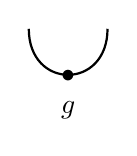
\begin{tikzpicture}
    \begin{knot}
      \strand[thick] (0,0)
        to [out=down,in=down,looseness=2] (1,0);
    \end{knot}
    \node[label=below:{$g$}] at (0.5,-0.6) {$\bullet$};
  \end{tikzpicture}
\] and \[
  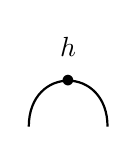
\begin{tikzpicture}
    \begin{knot}
      \strand[thick] (0,0)
        to [out=up,in=up,looseness=2] (1,0);
    \end{knot}
    \node[label=above:{$h$}] at (0.5,0.57) {$\bullet$};
  \end{tikzpicture}
\] respectively. We demand that \[
  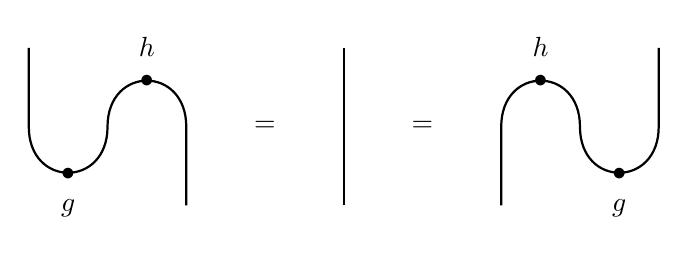
\begin{tikzpicture}
    \begin{scope}[xscale=-1,shift={(-2,0)}]
      \begin{knot}
        \strand[thick] (0,0)
        to (0,1)
        to [out=up,in=up,looseness=2] (1,1)
        to [out=down,in=down,looseness=2] (2,1)
        to (2,2);
      \end{knot}
      \node[label=above:{$h$}] at (0.5,1.57) {$\bullet$};
      \node[label=below:{$g$}] at (1.5,0.4) {$\bullet$};
    \end{scope}
    \node at (3,1) {$=$};
    \begin{scope}[shift={(4,0)}]
      \begin{knot}
        \strand[thick] (0,0) to (0,2);
      \end{knot}
    \end{scope}
    \node at (5,1) {$=$};
    \begin{scope}[shift={(6,0)}]
      \begin{knot}
        \strand[thick] (0,0)
        to (0,1)
        to [out=up,in=up,looseness=2] (1,1)
        to [out=down,in=down,looseness=2] (2,1)
        to (2,2);
      \end{knot}
      \node[label=above:{$h$}] at (0.5,1.57) {$\bullet$};
      \node[label=below:{$g$}] at (1.5,0.4) {$\bullet$};
    \end{scope}
  \end{tikzpicture}
\] which says that the bilinear form \(g\) is nondegenerate. To get
further, we'll also demand that \[
  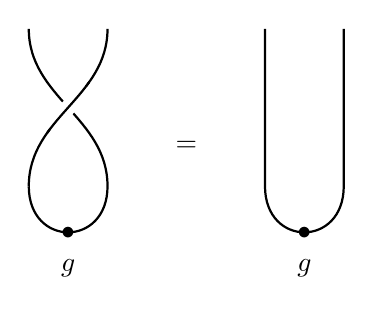
\begin{tikzpicture}
    \begin{knot}[clip width=7]
      \strand[thick] (0,0)
        to [out=down,in=up] (1,-2)
        to [out=down,in=down,looseness=2] (0,-2);
      \strand[thick] (0,-2)
        to [out=up,in=down] (1,0);
      \flipcrossings{1}
    \end{knot}
    \node[label=below:{$g$}] at (0.5,-2.6) {$\bullet$};
    \node at (2,-1.5) {$=$};
    \begin{knot}
      \strand[thick] (3,0)
        to (3,-2)
        to [out=down,in=down,looseness=2] (4,-2)
        to (4,0);
    \end{knot}
    \node[label=below:{$g$}] at (3.5,-2.6) {$\bullet$};
  \end{tikzpicture}
\] This says that the bilinear form \(g\) is symmetric, that is:
\[g(x,y) = g(y,x).\] But we can only state this equation if we're in a
monoidal category where we can ``switch arguments'', which in pictures
goes like this: \[
  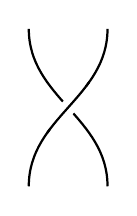
\begin{tikzpicture}
    \begin{knot}[clip width=7]
      \strand[thick] (0,0)
        to [out=down,in=up] (1,-2);
      \strand[thick] (0,-2)
        to [out=up,in=down] (1,0);
      \flipcrossings{1}
    \end{knot}
  \end{tikzpicture}
\] A monoidal category with this feature is called a ``symmetric
monoidal category'' (or more generally a ``braided monoidal category'',
but I don't want to get into those complications here).

So far, so good! The second problem is figuring out how to state the
condition \(|xy| = |x| |y|\). If we translate this into a condition on
our bilinear form \(g\), we get \[g(xy,xy) = g(x,x) g(y,y)\] An algebra
with a nondegenerate bilinear form having this property is called a
``composition algebra''. Hurwitz showed that such an algebra must have
dimension 1, 2, 4, or 8. However, there are examples other than the
famous four, coming from bilinear forms \(g\) that aren't positive
definite. For example, there are the ``split quaternions'' in dimension
4, or the ``split octonions'' in dimension 8.

Now, the problem with the above equational law is that it involves
duplication of arguments. But we can get around this problem by a
standard trick called ``polarization'', which people use a lot in
quantum mechanics.

First let's polarize the argument \(x\). To do this, note that we have
\[
  \begin{aligned}
    g(xy,xy) &= g(x,x) g(y,y)
  \\g(x'y,x'y) &= g(x',x') g(y,y)
  \end{aligned}
\] and also \[g((x+x')y,(x+x')y) = g(x+x',x+x') g(y,y).\] Subtracting
the first two equations from the last and then dividing by \(2\), we get
\[g(xy,x'y) = g(x,x') g(y,y).\] See? We've eliminated the duplication of
the argument \(x\). This new equation obviously implies the original
one.

Next we polarize the argument \(y\). We have \[
  \begin{aligned}
    g(xy,x'y) &= g(x,x') g(y,y)
  \\g(xy',x'y') &= g(x,x') g(y',y')
  \end{aligned}
\] and also \[g(x(y+y'),x'(y+y')) = g(x,x') g(y+y',y+y').\] Subtracting
the first two equations from the last one, we get
\[g(xy,x'y') + g(xy',x'y) = 2 g(x,x') g(y,y')\] Now there is no
duplication of arguments. We've paid a price, though: now our equation
involves addition, so we can only write it down if our category has the
extra feature that we can add morphisms. For this, we want our category
to be ``additive''.

So: the right doctrine in which to define composition algebras is the
doctrine of symmetric monoidal additive categories!

(Technical note: here we want the monoidal and additive structures to
get along nicely: tensoring of morphisms should be bilinear.)

Let me summarize by giving all the details. A ``composition object'' is
an object \(A\) in a symmetric monoidal additive category which is
equipped with morphisms \[
  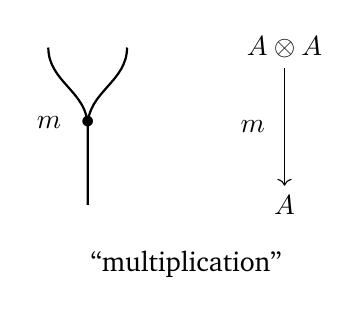
\begin{tikzpicture}
    \begin{knot}
      \strand[thick] (0,0)
        to [out=down,in=up] (0.5,-1)
        to (0.5,-2);
      \strand[thick] (1,0)
        to [out=down,in=up] (0.5,-1);
    \end{knot}
    \node[label=left:{$m$}] at (0.5,-0.95) {$\bullet$};
    \node (s) at (3,0) {$A\otimes A$};
    \node (t) at (3,-2) {$A$};
    \draw[->] (s) to node[label=left:{$m$}]{} (t);
    \node at (1.75,-2.75) {``multiplication''};
  \end{tikzpicture}
  \qquad\qquad
  \begin{tikzpicture}
    \begin{knot}
      \strand[thick] (0,0)
        to (0,-2);
    \end{knot}
    \node[label=left:{$i$}] at (0,0) {$\bullet$};
    \node (s) at (2,0) {$I$};
    \node (t) at (2,-2) {$A$};
    \draw[->] (s) to node[label=left:{$i$}]{} (t);
    \node at (1,-2.75) {``unit''};
  \end{tikzpicture}
\] \[
  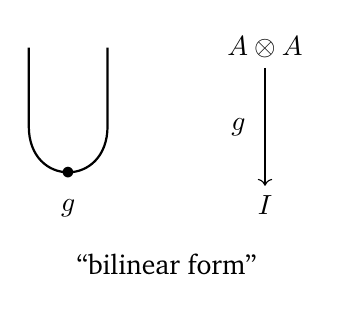
\begin{tikzpicture}
    \begin{knot}
      \strand[thick] (0,0)
        to (0,-1)
        to [out=down,in=down,looseness=2] (1,-1)
        to (1,0);
    \end{knot}
    \node[label=below:{$g$}] at (0.5,-1.6) {$\bullet$};
    \node (s) at (3,0) {$A\otimes A$};
    \node (t) at (3,-2) {$I$};
    \draw[->] (s) to node[label=left:{$g$}]{} (t);
    \node at (1.75,-2.75) {``bilinear form''};
  \end{tikzpicture}
  \qquad\qquad
  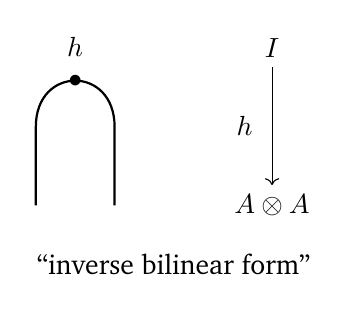
\begin{tikzpicture}
    \begin{knot}
      \strand[thick] (0,-2)
        to (0,-1)
        to [out=up,in=up,looseness=2] (1,-1)
        to (1,-2);
    \end{knot}
    \node[label=above:{$h$}] at (0.5,-0.43) {$\bullet$};
    \node (s) at (3,0) {$I$};
    \node (t) at (3,-2) {$A\otimes A$};
    \draw[->] (s) to node[label=left:{$h$}]{} (t);
    \node at (1.75,-2.75) {``inverse bilinear form''};
  \end{tikzpicture}
\] satisfying the equations already shown: \[
  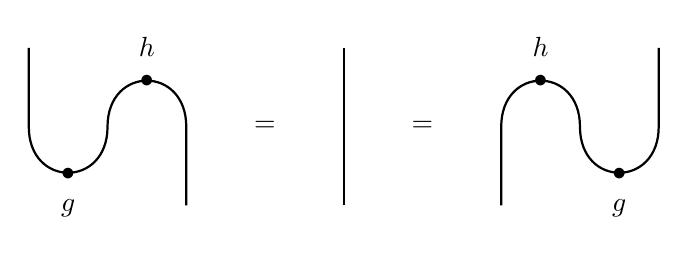
\begin{tikzpicture}
    \begin{scope}[xscale=-1,shift={(-2,0)}]
      \begin{knot}
        \strand[thick] (0,0)
        to (0,1)
        to [out=up,in=up,looseness=2] (1,1)
        to [out=down,in=down,looseness=2] (2,1)
        to (2,2);
      \end{knot}
      \node[label=above:{$h$}] at (0.5,1.57) {$\bullet$};
      \node[label=below:{$g$}] at (1.5,0.4) {$\bullet$};
    \end{scope}
    \node at (3,1) {$=$};
    \begin{scope}[shift={(4,0)}]
      \begin{knot}
        \strand[thick] (0,0) to (0,2);
      \end{knot}
    \end{scope}
    \node at (5,1) {$=$};
    \begin{scope}[shift={(6,0)}]
      \begin{knot}
        \strand[thick] (0,0)
        to (0,1)
        to [out=up,in=up,looseness=2] (1,1)
        to [out=down,in=down,looseness=2] (2,1)
        to (2,2);
      \end{knot}
      \node[label=above:{$h$}] at (0.5,1.57) {$\bullet$};
      \node[label=below:{$g$}] at (1.5,0.4) {$\bullet$};
    \end{scope}
  \end{tikzpicture}
\] and \[
  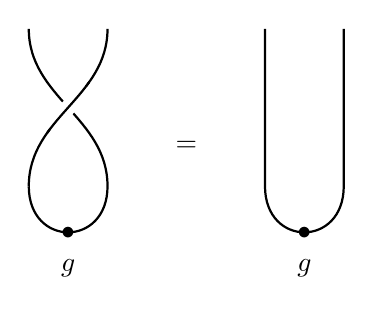
\begin{tikzpicture}
    \begin{knot}[clip width=7]
      \strand[thick] (0,0)
        to [out=down,in=up] (1,-2)
        to [out=down,in=down,looseness=2] (0,-2);
      \strand[thick] (0,-2)
        to [out=up,in=down] (1,0);
      \flipcrossings{1}
    \end{knot}
    \node[label=below:{$g$}] at (0.5,-2.6) {$\bullet$};
    \node at (2,-1.5) {$=$};
    \begin{knot}
      \strand[thick] (3,0)
        to (3,-2)
        to [out=down,in=down,looseness=2] (4,-2)
        to (4,0);
    \end{knot}
    \node[label=below:{$g$}] at (3.5,-2.6) {$\bullet$};
  \end{tikzpicture}
\] together with the left and right unit laws: \[
  \begin{tikzpicture}
    \begin{knot}
      \strand[thick] (0,0.5) to (0,0);
      \strand[thick] (1,1.5) to (1,0);
      \strand[thick] (0,0)
        to [out=down,in=up] (0.5,-1)
        to (0.5,-2);
      \strand[thick] (1,0)
        to [out=down,in=up] (0.5,-1);
    \end{knot}
    \node[label=left:{$i$}] at (0,0.5) {$\bullet$};
    \node[label=left:{$m$}] at (0.5,-0.95) {$\bullet$};
    \node at (2,-0.25) {$=$};
    \begin{knot}
      \strand[thick] (3,1.5) to (3,-2);
    \end{knot}
    \node at (4,-0.25) {$=$};
    \begin{scope}[xscale=-1,shift={(-6,0)}]
      \begin{knot}
        \strand[thick] (0,0.5) to (0,0);
        \strand[thick] (1,1.5) to (1,0);
        \strand[thick] (0,0)
          to [out=down,in=up] (0.5,-1)
          to (0.5,-2);
        \strand[thick] (1,0)
          to [out=down,in=up] (0.5,-1);
      \end{knot}
      \node[label=right:{$i$}] at (0,0.5) {$\bullet$};
      \node[label=left:{$m$}] at (0.5,-0.95) {$\bullet$};
    \end{scope}
  \end{tikzpicture}
\] and best of all, the equation
\[g(xy,x'y') + g(xy',x'y) = 2 g(x,x') g(y,y')\] translated into pictures
like this: \[
  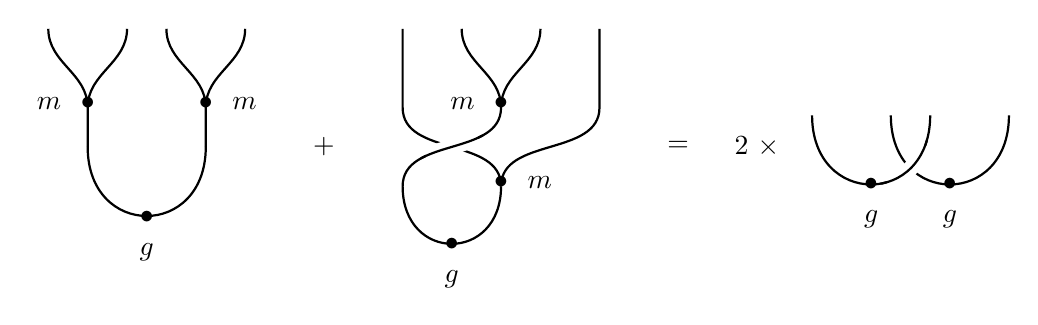
\begin{tikzpicture}
    \begin{knot}
      \strand[thick] (0,0)
        to [out=down,in=up] (0.5,-1)
        to (0.5,-1.5);
      \strand[thick] (1,0)
        to [out=down,in=up] (0.5,-1);
      \strand[thick] (1.5,0)
        to [out=down,in=up] (2,-1)
        to (2,-1.5);
      \strand[thick] (2.5,0)
        to [out=down,in=up] (2,-1);
      \strand[thick] (0.5,-1.5)
        to [out=down,in=down,looseness=2] (2,-1.5);
    \end{knot}
    \node[label=left:{$m$}] at (0.5,-0.95) {$\bullet$};
    \node[label=right:{$m$}] at (2,-0.95) {$\bullet$};
    \node[label=below:{$g$}] at (1.25,-2.4) {$\bullet$};
    \node at (3.5,-1.5) {$+$};
    \begin{scope}[shift={(4.5,0)}]
      \begin{knot}[clip width=7]
        \strand[thick] (0,0)
          to (0,-1)
          to [out=down,in=up] (1.25,-2);
        \strand[thick] (0.75,0)
          to [out=down,in=up] (1.25,-1)
          to [out=down,in=up] (0,-2)
          to [out=down,in=down,looseness=2] (1.25,-2);
        \strand[thick] (1.75,0)
          to [out=down,in=up] (1.25,-1);
        \strand[thick] (2.5,0) to (2.5,-1)
          to [out=down,in=up] (1.25,-2);
        \flipcrossings{1}
      \end{knot}
      \node[label=left:{$m$}] at (1.25,-0.95) {$\bullet$};
      \node[label=right:{$m$}] at (1.25,-1.95) {$\bullet$};
      \node[label=below:{$g$}] at (0.625,-2.74) {$\bullet$};
    \end{scope}
    \node at (8,-1.5) {$=$};
    \node at (9,-1.5) {$2\,\,\times$};
    \begin{scope}[shift={(9.7,-1.1)}]
      \begin{knot}[clip width=7]
        \strand[thick] (0,0)
          to [out=down,in=down,looseness=2] (1.5,0);
        \strand[thick] (1,0)
          to [out=down,in=down,looseness=2] (2.5,0);
      \end{knot}
      \node [label=below:{$g$}] at (0.75,-0.88) {$\bullet$};
      \node [label=below:{$g$}] at (1.75,-0.88) {$\bullet$};
    \end{scope}
  \end{tikzpicture}
\]

Now, given all this stuff, we can define the ``dimension'' of our
composition algebra to be the value of this morphism from \(I\) to
\(I\): \[
  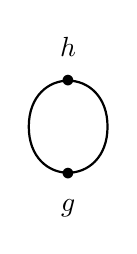
\begin{tikzpicture}
    \begin{knot}
      \strand[thick] (0,0)
        to [out=up,in=up,looseness=2] (1,0)
        to [out=down,in=down,looseness=2] (0,0);
    \end{knot}
    \node[label=above:{$h$}] at (0.5,0.57) {$\bullet$};
    \node[label=below:{$g$}] at (0.5,-0.6) {$\bullet$};
  \end{tikzpicture}
\] This reduces to the usual dimension of the algebra \(A\) when we're
in the category \(\mathsf{Vect}\). Of course, only in certain categories
is this dimension bound to be a \emph{number} --- namely, those
categories where every morphism from \(I\) to \(I\) is some number times
the identity morphism.

By making an extra assumption like this, Boos is able to give a
``picture proof'' that in a large class of symmetric monoidal additive
categories, every composition object has dimension 1, 2, 4 or 8. This is
great, because it means we can talk about things like real, complex,
quaternionic and octonionic objects in a wide variety of categories! He
doesn't prove such objects exist, but I think this should be easy, at
least with some extra assumptions which would allow us to construct them
``by hand'', mimicking standard constructions of the normed division
algebras.

But now I must warn you of some things. Boos doesn't state his result
the way I would! Instead of working with ``composition objects'' (which
appear to be my own invention), he works with ``vector product
algebras''. These are modelled, not after the normed division algebras
themselves, but after their ``imaginary parts''. These have both an
inner product and a ``vector product''.

For example, the imaginary quaternions form a \(3\)-dimensional vector
product algebra with vector product given by
\[a\times b = \frac12(ab - ba).\] This is just the usual cross product!
The same formula makes the imaginary octonions into a \(7\)-dimensional
vector product algebra, the imaginary complex numbers into a boring
\(1\)-dimensional one\ldots{} and the imaginary real numbers into an
even more boring 0-dimensional one.

Boos writes down the axioms for a vector product algebra using pictures
much like I just did for a composition object, and he shows that under
some pretty mild conditions you can freely go back and forth between the
two concepts.

I think you can summarize his theorem on vector product algebras as
follows: in all symmetric monoidal \(R\)-linear categories where \(R\)
is a commutative ring containing \(\mathbb{Z}[\frac12]\) and \(I\) is a
simple object, vector product algebras must have dimension 0, 1, 3, or
7. He doesn't state his result quite this way, but I'm pretty sure
that's what it boils down to. As for the jargon: a category is
``\(R\)-linear'' if the homsets are \(R\)-modules and composition of
morphisms is bilinear; for monoidal categories we also want tensoring
morphisms to be bilinear. The ring \(\mathbb{Z}[\frac12]\) consists of
all fractions with a power of 2 in the denominator --- Boos needs this
because he needs to divide by \(2\) at some point in his argument. For
an \(R\)-linear category, an object \(I\) is ``simple'' if
\(\operatorname{Hom}(I,I) = R\). This allows us to interpret the
dimension of our vector product algebra as an element of \(R\) --- which
Boos shows is actually one of the integers 0, 1, 3, or 7.

Let me conclude by showing you Boos' main axiom for vector product
algebras, written in terms of pictures: \[
  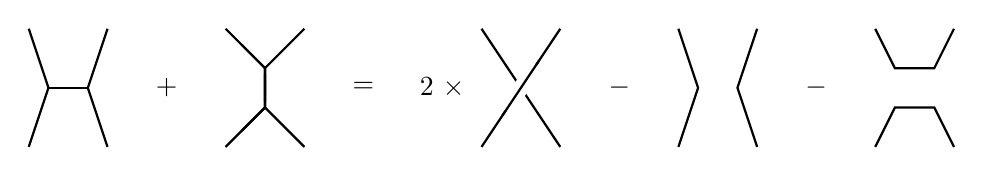
\begin{tikzpicture}
    \begin{knot}[clip width=0]
      \strand[thick] (0,0)
        to (0.25,-0.75)
        to (0,-1.5);
      \strand[thick] (1,0)
        to (0.75,-0.75)
        to (1,-1.5);
      \strand[thick] (0.25,-0.75) to (0.75,-0.75);
    \end{knot}
    \node at (1.75,-0.75) {$+$};
    \begin{scope}[shift={(2.5,0)}]
      \begin{knot}[clip width=0]
        \strand[thick] (0,0)
          to (0.5,-0.5)
          to (0.5,-1)
          to (0,-1.5);
        \strand[thick] (1,0)
          to (0.5,-0.5)
          to (0.5,-1)
          to (1,-1.5);
      \end{knot}
    \end{scope}
    \node at (4.25,-0.75) {$=$};
    \node at (5.25,-0.75) {$2\,\,\times$};
    \begin{scope}[shift={(5.75,0)}]
      \begin{knot}[clip width=7]
        \strand[thick] (0,0) to (1,-1.5);
        \strand[thick] (1,0) to (0,-1.5);
        \flipcrossings{1}
      \end{knot}
    \end{scope}
    \node at (7.5,-0.75) {$-$};
    \begin{scope}[shift={(8.25,0)}]
      \begin{knot}
        \strand[thick] (0,0)
          to (0.25,-0.75)
          to (0,-1.5);
        \strand[thick] (1,0)
          to (0.75,-0.75)
          to (1,-1.5);
      \end{knot}
    \end{scope}
    \node at (10,-0.75) {$-$};
    \begin{scope}[shift={(10.75,0)}]
      \begin{knot}
        \strand[thick] (0,0)
          to (0.25,-0.5)
          to (0.75,-0.5)
          to (1,0);
        \strand[thick] (0,-1.5)
          to (0.25,-1)
          to (0.75,-1)
          to (1,-1.5);
      \end{knot}
    \end{scope}
  \end{tikzpicture}
\] Ain't it cool? Fans of knot theory will be struck by the resemblance
to various ``skein relations''. Fans of physics will be reminded of
Feynman diagrams. But what is the secret inner meaning?

\begin{center}\rule{0.5\linewidth}{0.5pt}\end{center}

\begin{quote}
\emph{``The perplexity of life arises from there being too many
interesting things in it for us to be interested properly in any of
them.''}

--- G. K. Chesterton, 1909
\end{quote}



\hypertarget{week170}{%
\section{August 8, 2001}\label{week170}}

I've been travelling around a lot lately. For a couple of weeks I was in
Turkey, resisting the lure of the many internet cafes. I urge you all to
visit Istanbul when you get a chance! Fascinating music fills the
streets. There are a lot of nice bookstore-cafes on Istiklal Caddesi
near Taksim Square, and a huge number of musical instrument shops at the
other end of this street, down near Tunel Square. I bought a nice
doumbek at one of these shops, and looked at lots of ouzes, sazes and
neys, none of which I can play. It's also imperative to check out the
Grand Bazaar, the mosques, and the Topkapi Palace --- the harem there
has most beautiful geometric tiling patterns I've ever seen. I'm not
sure why that's true; perhaps this is where the sultans spent most of
their time.

The mathematics of tilings is a fascinating subject, but that's not what
I'm going to talk about. After my trip to Turkey, I went to a conference
at Stanford:

\begin{enumerate}
\def\labelenumi{\arabic{enumi})}
\tightlist
\item
  Conference on Algebraic Topological Methods in Computer Science,
  Stanford University, \texttt{http://math.stanford.edu/atmcs/index.htm}
\end{enumerate}

There were lots of fun talks, but I'll just mention two.

The talk most related to physics was the one by my friend Dan
Christensen, who spoke on ``Spin Networks, Spin Foams and Quantum
Gravity'', describing a paper he is writing with Greg Egan on efficient
algorithms for computing Riemannian \(10j\) symbols. Dan is a homotopy
theorist at the University of Western Ontario, and Greg is my favorite
science fiction writer. They're both interested in quantum gravity, and
they're both good at programming. Together with some undergraduate
students of Dan's, the three of us are starting to study the Riemannian
and Lorentzian Barrett-Crane models of quantum gravity with the help of
computer simulations. But to get anywhere with this, we need to get good
at computing ``\(10j\) symbols''.

Huh? ``\(10j\) symbols''??

Well, as with any quantum field theory, the key to the Barrett-Crane
model is the partition function. In the Riemannian version of this
theory, you compute the partition function as follows. First you take
your \(4\)-dimensional manifold representing spacetime and triangulate
it. Then you label all the triangles by spins
\(j = 0, 1/2, 1, 3/2, \ldots\). Following certain specific formulas you
then calculate a number for each 4-simplex, a number for each
tetrahedron, and a number for each triangle, using the spin labellings.
Then you multiply all these together. Finally you sum over all
labellings to get the partition function. The only tricky part is the
convergence of this sum, which was proved by Perez:

\begin{enumerate}
\def\labelenumi{\arabic{enumi})}
\setcounter{enumi}{1}
\tightlist
\item
  Alejandro Perez, ``Finiteness of a spin foam model for euclidean
  quantum general relativity'', \emph{Nucl. Phys.} \textbf{B599} (2001)
  427--434. Also available as
  \href{https://arxiv.org/abs/gr-qc/0011058}{\texttt{gr-qc/0011058}}.
\end{enumerate}

The most interesting aspect of all this is the formula giving numbers
for \(4\)-simplices. A \(4\)-simplex has 10 triangular faces all of
which get labelled by spins, and the formula says how to compute a
number from these 10 spins --- the so-called ``\(10j\) symbol''.

How do you compute \(10j\) symbols? One approach involves representation
theory, or in lowbrow terms, multiplying a bunch of matrices.
Unfortunately, if you go about this in the most simple-minded obvious
fashion, when the spins labelling your triangles are all about equal to
\(j\), you wind up needing to work with matrices that are as big as
\(N\times N\), where \[N = (2j+1)^{12}.\] If you do this, already for
\(j = 1/2\) you are dealing with square matrices that are \(2^{12}\) by
\(2^{12}\). This is too big to be practical!

In computer science lingo, this algorithm sucks because it uses
\(\mathcal{O}(j^{12})\) time and also \(\mathcal{O}(j^{12})\) space. You
might think it was \(\mathcal{O}(j^{24})\), but it's not that
bad\ldots{} however, it's still very bad!

Luckily, Dan and Greg have figured out a much more efficient algorithm,
which uses only \(\mathcal{O}(j^6)\) time and \(\mathcal{O}(j)\) space.
Alternatively, with more caching of data, they can get
\(\mathcal{O}(j^5)\) time and \(\mathcal{O}(j^3)\) space, or maybe even
better. Using an algorithm of this sort, Dan can compute the \(10j\)
symbol for spins up to 55. For all spins equal to 55, the calculation
took about 10 hours on a normal desktop computer. However, for computing
partition functions it appears that small spins are much more important,
and then the computation takes milliseconds.

(Actually, for computing partition functions, Dan is not using a
desktop: he is using a Beowulf cluster, which is a kind of supercomputer
built out of lots of PCs. This works well for partition functions
because the computation is highly parallelizable.)

John Barrett has also figured out a very different approach to computing
\(10j\) symbols:

\begin{enumerate}
\def\labelenumi{\arabic{enumi})}
\setcounter{enumi}{2}
\tightlist
\item
  John W. Barrett, ``The classical evaluation of relativistic spin
  networks'', \emph{Adv. Theor. Math. Phys.} \textbf{2} (1998),
  593--600. Also available as
  \href{https://arxiv.org/abs/math.QA/9803063}{\texttt{math.QA/9803063}}.
\end{enumerate}

In this approach one computes the \(10j\) symbols by doing an integral
over the space of geometries of a \(4\)-simplex --- or more precisely,
over a product of 5 copies of the 3-sphere, where a point on one of
these 3-spheres describes the normal vector to one of the 5 tetrahedral
faces of the \(4\)-simplex.

Dan and Greg have also written programs that calculate the \(10j\)
symbols by doing these integrals. The answers agree with their other
approach.

We've already been getting some new physical insights from these
calculations. If you write down the integral formula for the Riemannian
\(10j\) symbols, a stationary phase argument due to John Barrett and
Ruth Williams suggests that, at least in the limit of large spins, the
dominant contribution to the integral for the \(10j\) symbol comes from
4-simplices whose face areas are the 10 spins in your \(10j\) symbols:

\begin{enumerate}
\def\labelenumi{\arabic{enumi})}
\setcounter{enumi}{3}
\tightlist
\item
  John W. Barrett and Ruth M. Williams, ``The asymptotics of an
  amplitude for the \(4\)-simplex'', \emph{Adv. Theor. Math. Phys.}
  \textbf{3} (1999), 209--215. Also available as
  \href{https://arxiv.org/abs/gr-qc/9809032}{\texttt{gr-qc/9809032}}.
\end{enumerate}

However, Dan and Greg's calculations suggest instead that the dominant
contribution comes from certain ``degenerate'' configurations. Some of
these correspond to points on the product of 5 copies of the 3-sphere
that are close to points of the form \((v,v,v,v,v)\) --- or roughly
speaking, 4-simplices whose 5 normal vectors are all pointing the same
way. Others come from sprinkling minus signs in this list of vectors.
Heuristically, we can think of these degenerate configurations as
extremely flattened-out \(4\)-simplices.

For simplicity, we have concentrated so far on studying the \(10j\)
symbols in the case when all 10 spins are equal. In this case we can
show that the only nondegenerate \(4\)-simplex with these spins as face
areas is the regular \(4\)-simplex (all of whose faces are congruent
equilateral triangles). Greg used stationary phase to compute the
contribution of this regular \(4\)-simplex to Barrett's integral formula
for the \(10j\) symbols, and it turned out that asymptotically, for
large \(j\), this contribution decays like \(j^{-9/2}\). On the other
hand, Dan's numerical computations of the \(10j\) symbol suggests that
it goes like \(j^{-2}\). This suggests that for large \(j\), the
contribution of the regular \(4\)-simplex is dwarfed by that of the
degenerate \(4\)-simplices.

Greg has gotten more evidence for this by studying the integral formula
for the \(10j\) symbols and estimating the contribution due to
degenerate 4-simplices. This estimate indeed goes like \(j^{-2}\) for
large \(j\).

There is a lot more to be understood here, but plunging ahead
recklessly, we can ask what all this means for the physics of the
Barrett-Crane model. For example: is the dominant contribution to the
partition function going to come from spacetime geometries with lots of
degenerate \(4\)-simplices?

I think that's a premature conclusion, because we already have evidence
that 4 -simplices with large face areas are not contributing that much
compared to those with small face areas when we compute the partition
function as a sum over spin foams. In other words, it seems that in the
Riemannian Barrett-Crane model, spacetime is mostly made of lots of
small \(4\)-simplices, rather than a few giant ones. If so, the tendency
for the giant ones to flatten out may not be so bad.

Of course the really important thing will be to study these questions
for the Lorentzian theory, but it's good to look at the Riemannian
theory too.

Another talk on a subject close to my heart was given by Noson Yanofsky.
It was based on these papers of his, especially the last:

\begin{enumerate}
\def\labelenumi{\arabic{enumi})}
\setcounter{enumi}{4}
\item
  Noson S. Yanofsky, ``Obstructions to coherence: natural noncoherent
  associativity'', \emph{Jour. Pure Appl. Alg.} \textbf{147} (2000),
  175--213. Also available at
  \href{https://arxiv.org/abs/math.QA/9804106}{\texttt{math.QA/9804106}}.

  ``The syntax of coherence''. To appear in \emph{Cahiers Top. Geom.
  Diff.}. Also available at
  \href{https://arxiv.org/abs/math.CT/9910006}{\texttt{math.CT/9910006}}.

  ``Coherence, homotopy and 2-theories''. To appear in \emph{K-Theory}.
  Also available at
  \href{https://arxiv.org/abs/math.CT/0007033}{\texttt{math.CT/0007033}}.
\end{enumerate}

One of the cool things Yanofsky has done is to study what happens when
we categorify Lawvere's concept of an ``algebraic theory''. I've already
explained this idea of ``algebraic theory'' in
\protect\hyperlink{week53}{``Week 53''} and
\protect\hyperlink{week136}{``Week 136''}, so I'll just quickly recap it
here:

The notion of ``algebraic theory'' is just a slick way to study sets
equipped with extra algebraic structure. We call a category
\(\mathcal{C}\) with finite products an ``algebraic theory'' if its
objects are all of the form \(1, X, X^2, X^3, \ldots\) for some
particular object \(X\). We call a product-preserving functor
\(F\colon\mathcal{C}\to\mathsf{Set}\) a ``model'' of the theory. And we
call a natural transformation between such functors a ``homomorphism''
between models. This gives us a category \(\mathsf{Mod}(\mathcal{C})\)
consisting of models and homomorphisms between them, and it turns out
that many categories of algebraic gadgets are of this form: the category
of monoids, the category of groups, the category of abelian groups, and
so on.

Since algebraic theories are good for studying sets with extra algebraic
structure, we might hope that by categorifying, we could obtain a
concept of ``algebraic 2-theories'' which is good for studying
\emph{categories} with extra algebraic structure. And it's true! In
1974, John Gray defined an ``algebraic 2-theory'' to be a \(2\)-category
\(\mathcal{C}\) with finite products, all of whose objects are of the
form \(1, X, X^2, X^3,\ldots\) for some particular object \(X\). Define
a ``model'' of this 2-theory to be a product-preserving 2-functor
\(F\colon\mathcal{C}\to\mathsf{Cat}\). And define a ``homomorphism''
between models to be a pseudonatural transformation between such
2-functors.

Huh? ``Pseudonatural''??

Sorry, now things are getting a bit technical: the right thing going
between 2-functors is not a natural transformation but something a bit
weaker called a ``pseudonatural transformation'', where the usual
commuting squares in the definition of a natural transformation are
required to commute only up to certain specified 2-isomorphisms, which
in turn satisfy some coherence laws described here:

\begin{enumerate}
\def\labelenumi{\arabic{enumi})}
\setcounter{enumi}{5}
\tightlist
\item
  G. Maxwell Kelly and Ross Street, \emph{Review of the elements of
  \(2\)-categories}, Springer Lecture Notes in Mathematics \textbf{420},
  Berlin, 1974, pp.~75--103.
\end{enumerate}

However, you don't need to understand the details right now. There is
also something going between pseudonatural transformations called a
``modification'', and this gives us ``2-homomorphisms'' between
homomorphisms between models of our algebraic theory. Thanks to these
there is a \(2\)-category \(\mathsf{Mod}(\mathcal{C})\) consisting of
models of our 2-theory homomorphisms between those, and 2-homomorphisms
between those.

Some examples might help! For example, there's a 2-theory
\(\mathcal{C}\) called the ``theory of weak monoidal categories''.
Models of \(\mathcal{C}\) are weak monoidal categories, homomorphisms
are monoidal functors, and 2-homomorphisms are natural transformations,
so \(\mathsf{Mod}(\mathcal{C})\) is the usual \(2\)-category of monoidal
\(2\)-categories. There's a similar 2-theory \(\mathcal{C}'\) called
``the theory of strict monoidal categories'', for which
\(\mathsf{Mod}(\mathcal{C}')\) is the usual \(2\)-category of strict
monoidal categories.

(Hyper-technical note for \(n\)-category mavens only: in both examples
here, monoidal functors are required to preserve unit and tensor product
only \emph{up to coherent natural isomorphism}. This nuance is what we
get from working with pseudonatural rather than natural transformations.
Without this nuance, some of the stuff I'm about to say would be false.)

Now, whenever we have a product-preserving 2-functor between 2-theories,
say \(F\colon\mathcal{C}\to\mathcal{C}'\), we get an induced 2-functor
going the other way,
\[F^*\colon\mathsf{Mod}(\mathcal{C}')\to\mathsf{Mod}(\mathcal{C}).\] For
example, there's a product-preserving 2-functor from the theory of weak
monoidal categories to the theory of strict monoidal categories, and
this lets us turn any strict monoidal category into a weak one.

Now in this particular example, \(F^*\) is a biequivalence, which is the
nice way to say that the \(2\)-categories \(\mathsf{Mod}(C)\) and
\(\mathsf{Mod}(C')\) are ``the same'' for all practical purposes. And in
fact, saying that this particular \(F^*\) is a biequivalence is really
just an ultra-slick version of Mac Lane's theorem --- the theorem we use
to turn weak monoidal categories into strict ones.

Now, Mac Lane's theorem is the primordial example of a ``strictification
theorem'' --- a theorem that lets us turn ``weak'' algebraic structures
on categories into ``strict'' ones, where lots of isomorphisms, like the
associators in the monoidal category example, are assumed to be
equations. This suggests that lots of coherence theorems can be stated
by saying that 2-functors of the form \(F^*\) are biequivalences.

So: is there a super-general strictification theorem where we can start
from any 2-theory \(\mathcal{C}\) and get a ``strictified'' version
\(\mathcal{C}'\) together with an \(F\colon\mathcal{C}\to\mathcal{C}'\)
such that \(F^*\) is a biequivalence?

As a step in this direction, Yanofsky has cooked up a model category of
algebraic 2-theories, in which \(F\colon\mathcal{C}\to\mathcal{C}'\) is
a weak equivalence precisely when \(F^*\) is a biequivalence.

Huh? ``Model category''??

Well, if you don't know what a ``model category'' is, you're in serious
trouble now! They're a concept invented by Quillen for generalizing the
heck out of homotopy theory. Try reading his book:

\begin{enumerate}
\def\labelenumi{\arabic{enumi})}
\setcounter{enumi}{6}
\tightlist
\item
  Daniel G. Quillen, \emph{Homotopical Algebra}, Springer Lecture Notes
  in Mathematics, vol.~\textbf{43}, Springer, Berlin, 1967.
\end{enumerate}

or for something newer:

\begin{enumerate}
\def\labelenumi{\arabic{enumi})}
\setcounter{enumi}{7}
\tightlist
\item
  Mark Hovey, \emph{Model Categories}, American Mathematical Society
  Mathematical Surveys and Monographs, vol \textbf{63}, Providence,
  Rhode Island, 1999.
\end{enumerate}

or else:

\begin{enumerate}
\def\labelenumi{\arabic{enumi})}
\setcounter{enumi}{8}
\tightlist
\item
  Paul G. Goerss and John F. Jardine, \emph{Simplicial Homotopy Theory},
  Birkhauser, Boston, 1999.
\end{enumerate}

(By the way, Jardine was one of the organizers of this Stanford
conference, along with Gunnar Carlsson. He told me he had created a
hypertext version of this book, but has not been able to get the
publisher interested in it. Sad!)

Anyway, in the framework of model categories, the problem of
``strictifying'' an algebraic structure on categories then amounts to
finding a ``minimal model'' of a given 2-theory \(\mathcal{C}\) ---
roughly speaking, a weakly equivalent 2-theory with as little flab as
possible. The concept of ``minimal model'' is important in homotopy
theory, but apparently Yanofsky is the first to have given a general
definition of this concept applicable to any model category. Yanofsky
has not shown that every algebraic 2-theory admits a minimal model, but
this seems like a fun and interesting question.

\begin{center}\rule{0.5\linewidth}{0.5pt}\end{center}

\begin{quote}
\emph{all ignorance toboggans into know and trudges up to ignorance
again.}

--- e.e.cummings, 1959
\end{quote}



\hypertarget{week171}{%
\section{October 10, 2001}\label{week171}}

There isn't a Nobel prize for mathematics. You've probably heard why:
Alfred Nobel was annoyed that the famous mathematician Mittag-Leffler
had an affair with his wife. Well, that's what they say, anyway. It
makes a great story. The only problem is, Nobel was never married! So
it's just another urban legend. For more details, see:

\begin{enumerate}
\def\labelenumi{\arabic{enumi})}
\tightlist
\item
  Urban legends reference pages, ``The Prize's Rite'',
  \texttt{http://www.snopes2.com/science/nobel.htm}
\end{enumerate}

More likely, Nobel just didn't consider mathematics sufficiently
practical. In any event, mathematicians have always felt a bit grumpy
about this slight. Their adoption of the Fields Medal as a kind of
substitute has never been completely satisfying. For one thing, the
Fields Medal is only for work done before the age of 40 --- a condition
that seems ever more silly with the wisdom of age. For another, the
Fields prize gives you a measly 15,000 Canadian dollars, while the Nobel
prize keeps going up: this year, it was 10 million Swedish crowns, or
almost a million bucks.

Anyway, now there may be a better substitute: the Abel Prize.

\begin{itemize}
\tightlist
\item
  ``Norway Establishes Abel Prize in Mathematics'',
  \texttt{http://www.maa.org/news/abel\_prize.html}
\end{itemize}

It even almost rhymes with Nobel! Abel, of course, was a famous
Norwegian mathematician, and this prize will be awarded annually by the
government of Norway, starting in 2003. It will have a value of about
\$500,000, at least initially. Even better, it will be awarded on a
first-come, first-serve basis\ldots{} so send in your application now.

When I was in Cambridge this summer, I visited Tom Leinster and Eugenia
Cheng, who showed me around the new mathematics buildings. The Cambridge
system is too Byzantine for a mere American to understand, but there are
two main things resembling a ``mathematics department'': DPMSS, the
Department of Pure Mathematics and Mathematical Statistics, and DAMTP,
the Department of Applied Mathematics and Theoretical Physics. They used
to be in separate dilapidated buildings downtown on Silver Street, but
now they occupy two towers in a huge complex near the Newton Institute,
on the outskirts of town.

The new setup is pretty cool. Parts of it are still under construction,
but you can get the idea already. Different breeds of mathematicians
will be housed in different towers, all surrounding a central building
resembling an airplane hanger, which is actually an enormous cafeteria.
The univeral human interest in food will lure otherwise aloof
specialists to mingle and chat. I even saw Hawking there one day.
However, there is also a separate coffee lounge at the base of each
tower, so the different groups can have slightly more private chats.
Futuristic light sensors lower curtains in the cafeteria whenever the
sun comes out, to enhance the visitor's impression that it's always
cloudy in England. But the really cool thing is that every tower has a
door on the second floor which opens out to the \emph{roof} of the
cafeteria. The roof is covered with grass, like a little park! Finally,
people working on fluid dynamics are kept in the basement, which gurgles
mysteriously with the sound of experiments.

Leinster and Cheng are both students of Martin Hyland, and they both
work on \(n\)-categories. I've talked about their work before in
\protect\hyperlink{week165}{``Week 165''}. Leinster has just come out
with a nice paper on \(n\)-categories:

\begin{enumerate}
\def\labelenumi{\arabic{enumi})}
\tightlist
\item
  Tom Leinster, ``A survey of definitions of \(n\)-category'', available
  at
  \href{https://arxiv.org/abs/math.CT/0107188}{\texttt{math.CT/0107188}}.
\end{enumerate}

By now, there are lots of definitions of ``weak \(n\)-category'', and
our job is to understand how they're related. This paper is required
reading for anyone interested in this business: it goes through 10
different definitions, giving each definition in two pages and then
using two more pages to show how it works for \(n\) less than or equal
to 2. It also has a nice annotated bibliography giving some of the
history of the subject.

While I'm talking about review articles, here are some review articles
on quantum gravity:

\begin{enumerate}
\def\labelenumi{\arabic{enumi})}
\setcounter{enumi}{1}
\tightlist
\item
  Steve Carlip, ``Quantum gravity: a progress report'', \emph{Rep.~Prog.
  Phys.} \textbf{64} (2001) 885--942, also available at
  \href{https://arxiv.org/abs/gr-qc/0108040}{\texttt{gr-qc/0108040}}.
\end{enumerate}

This is an excellent \emph{long} description of where we stand on
quantum gravity, with a strong focus on the big conceptual problems.
Again, it's required reading for anyone in this field. It doesn't do
justice to string theory, which is a mammoth subject in its own. For
that, you might try this article which I bumped into in the same
journal:

\begin{enumerate}
\def\labelenumi{\arabic{enumi})}
\setcounter{enumi}{2}
\tightlist
\item
  Ulf Daniellson, ``Introduction to string theory'', \emph{Rep.~Prog.
  Phys.} \textbf{64} (2001) 51-96.
\end{enumerate}

It seems to do a pretty good job of the impossible --- explaining all of
string theory in less than 50 pages. Of course, if you want to get
serious, you'll eventually have to read some of the string theory
textbooks listed in \protect\hyperlink{week124}{``Week 124''} and
elsewhere.

There is also a new introduction to loop quantum gravity available
online. It's more of a book than an article:

\begin{enumerate}
\def\labelenumi{\arabic{enumi})}
\setcounter{enumi}{3}
\tightlist
\item
  Thomas Thiemann, \emph{Introduction to modern canonical quantum
  general relativity}, 301 pages, available at
  \href{https://arxiv.org/abs/gr-qc/0110034}{\texttt{gr-qc/0110034}}.
\end{enumerate}

This is really \emph{the} place to go if you want to catch up on the
last 15 years of work on loop quantum gravity. It's truly impressive.
It'll make fairly substantial demands on the average physicist's
mathematical know-how: for example, not just differential geometry,
which everyone into gravity must know, but also functional analysis.
Luckily, it has an appendix over 40 pages long which explains much of
the needed math. For the would-be grad student or postdoc, a very
helpful feature is the list of institutions where loop quantum gravity
is studied, in the Introduction.

Speaking of loop quantum gravity, here are a few interesting new papers
on that subject:

\begin{enumerate}
\def\labelenumi{\arabic{enumi})}
\setcounter{enumi}{4}
\item
  Rodolfo Gambini and Jorge Pullin, ``Consistent discretizations for
  classical and quantum general relativity'', available as
  \href{https://arxiv.org/abs/gr-qc/0108062}{\texttt{gr-qc/0108062}}.
\item
  Luca Bombelli, ``Statistical geometry of random weave states'',
  available as
  \href{https://arxiv.org/abs/gr-qc/0101080}{\texttt{gr-qc/0101080}}.
\item
  Michael Seifert, ``Angle and volume studies in quantized space'', 85
  pages, available as
  \href{https://arxiv.org/abs/gr-qc/0108047}{\texttt{gr-qc/0108047}}.
\end{enumerate}

The paper by Gambini and Pullin argues that good spin foam models will
come from quantizing ``consistent'' discretizations of general
relativity, that is, those where the discretized equations of motion
preserve the constraints on initial data, and where the solutions
converge to solutions of the continuum equations in the limit where the
discretization is made ever more fine.

The paper by Bombelli presents a proposal for states of loop quantum
gravity that should be good approximations to classical geometries. The
idea is to take a Riemannian manifold, sprinkle points on it randomly
form the corresponding Voronoi diagram, and label the edges with spins
in a certain way to get a spin network. If we then average over all
possible ways of randomly sprinkling these points, we get Bombelli's
``random weave state'' --- a kinematical state of quantum gravity that
approximates of the Riemannian geometry we started with.

I don't know if that made sense to you. Do you at least know what a
Voronoi diagram is? To explain that, a picture is worth a thousand
words, so I won't explain the concept --- I'll just urge you to play
with this applet:

\begin{enumerate}
\def\labelenumi{\arabic{enumi})}
\setcounter{enumi}{8}
\tightlist
\item
  Paul Chew, Voronoi/Delaunay Applet,
  \texttt{http://www.cs.cornell.edu/Info/People/chew/Delaunay.html}
\end{enumerate}

If you click the mouse to sprinkle the rectangle with points, you'll see
a bunch of edges appear, which intersect in vertices, forming a graph
called the Voronoi diagram. By epxerimenting a bit you can figure out
how it works --- or else you can cheat and read the text. You'll see
that generically the vertices of this graph are trivalent: they have
three edges coming out of them. If you click on the button that says
``Delaunay Triangulation'', you'll see the dual graph, which generically
consists of a bunch of triangles. Each edge of these triangles
intersects exactly one edge of the Voronoi diagram.

In the theory of quantum gravity where space is just \(2\)-dimensional
(a toy model), we can take the Voronoi diagram and label its edges by
spins \(j = 0, 1/2, 1, \ldots\) which match, as well as possible, the
lengths of the edge of the Delaunay triangulation which it intersects.
This will give us a spin network. Averaging over all ways of sprinking
the points, we then get Bombelli's ``random weave state''. The same sort
of idea works in higher dimensions, too.

Finally, Michael Seifert's paper is an excellent undergraduate thesis on
loop quantum gravity, done with the help of Seth Major. After a nice
review of the basics, it studies some operators that act on the Hilbert
space of states of a single spin network vertex: in particular, the
volume operator and some less familiar operators that measure the angles
between spin network edges. He proves some nice things about these, and
also gets some interesting numerical results --- which someone should
make into theorems. The relation between 3d geometry and the
representation theory of \(\mathrm{SU}(2)\) still has unexplored
wrinkles!



\hypertarget{week172}{%
\section{October 29, 2001}\label{week172}}

I recently went to a conference on ``Discrete Random Geometries and
Quantum Gravity'', organized by Renate Loll:

\begin{enumerate}
\def\labelenumi{\arabic{enumi})}
\tightlist
\item
  Discrete Random Geometries and Quantum Gravity,
  \texttt{http://www1.phys.uu.nl/Symposion/EUWorkshop.htm}
\end{enumerate}

She was one of the people who first gave me the courage to work on
quantum gravity. I'd been interested in it for a long time, but I didn't
like how string theory relied on supersymmetry and a background metric,
so I didn't know any approach that looked promising until I saw her give
a talk on loop quantum gravity at a conference in Seattle in the early
1990s. She was interested in numerical simulation of quantum gravity
models even back then, and by now she's one of the top experts on this
subject. But it's extremely hard to get permanent positions in quantum
gravity, especially in Europe, so I was happy when she recently got a
job at the University of Utrecht. To kick off her stay there, she threw
this conference!

I like to read ``Wired'' magazine when I'm on long airplane trips. On my
flight to Amsterdam, I found this interesting article:

\begin{enumerate}
\def\labelenumi{\arabic{enumi})}
\setcounter{enumi}{1}
\tightlist
\item
  Wil McCarthy, ``Ultimate alchemy'', \emph{Wired}, October 2001, 150.
\end{enumerate}

It's about people are using ``quantum dots'' to make ``artificial
atoms''. A quantum dot is a tiny speck of conductive material that can
be used as a potential well holding one or more electrons in a bound
state. Such bound states are a lot like atoms! However, the ones people
have made so far are about 50 times bigger than actual atoms, because
they are more loosely bound. This also means that they ionize more
easily, so they need to be kept very cold.

However, they can have more electrons than normal atoms, since they
aren't limited by the tendency of large nuclei to undergo radioactive
decay, or ultimately, somewhere around element 137, the tendency of
strong electric fields to ``spark the vacuum'' by creation of
particle-antiparticle pairs --- a quantum field theory effect that's not
included in the bare-bones Schroedinger equation. So, someday we may
learn how the periodic table goes up to, say, element 500! I've
sometimes imagined decadent future chemists studying such elements on
the computer, just for the fun of it\ldots{} but now perhaps they'll do
it with ``artificial atoms''.

Now, McCarthy is a science fiction writer, so he imagines more dramatic
applications of quantum dots, like ``programmable matter'' --- a gadget
whose surface can, say, turn from lead to gold at the flick of a switch.
Personally I don't see how to get these tricks to work at room
temperature until we make artificial atoms almost as small as real ones,
which I don't see how to do without them being\ldots{} atoms! But even
so, I believe there will be some cool technological applications of
quantum dots.

For more on quantum dots by experts on the subject, try these papers:

\begin{enumerate}
\def\labelenumi{\arabic{enumi})}
\setcounter{enumi}{2}
\item
  Marc Kastner, ``Artificial atoms'', \emph{Physics Today} \textbf{46}
  (1993), 24. Also available at
  \texttt{http://web.mit.edu/physics/people/marc\_kastner.htm}
\item
  Leo Kouwenhoven and Charles Marcus, ``Quantum dots'', \emph{Physics
  World}, June 1998. Also available at
  \texttt{http://marcuslab.harvard.edu/}
\end{enumerate}

Unfortunately I didn't have access to these papers on my flight from Los
Angeles to Amsterdam. It takes 10 hours, so I had to read a lot more to
keep from going insane with boredom. Even the latest news about
bioterrorism and bombings was not enough to keep me entertained. (By the
way, I predict that a highly contagious virus will sweep the United
States and kill about 20,000 people within the next few months. It's
called ``influenza'', and that's the average number of Americans who die
from it each year. I plan to call the FBI and warn them about this.)

So, I had to hit the serious mathematical physics:

\begin{enumerate}
\def\labelenumi{\arabic{enumi})}
\setcounter{enumi}{4}
\tightlist
\item
  Terry Gannon, ``Monstrous moonshine and the classification of CFT'',
  in \emph{Conformal Field Theory: New Non-Perturbative Methods in
  String and Field Theory}, Yavuz Nutku, Cihan Saclioglu and Teoman
  Turgut, eds., Perseus Publishing, 2000.
\end{enumerate}

This is a very pleasant 66-page review article on ``monstrous
moonshine'', which is what people call the relation between the Monster
group and modular forms. Someday I'll have to say a lot more about this;
for now see \protect\hyperlink{week66}{``Week 66''} if you have no idea
what I'm talking about. Gannon's article is full of juicy mathematical
tidbits and pieces of wisdom. He even gives a new explanation of why the
number 24 is so important throughout mathematics and string theory. If
\(x^2 = 1 \mod n\), then \(x\) must be relatively prime to \(n\)\ldots{}
and 24 is the largest integer for which the converse holds! Alas, Gannon
does not explain how this relates to the other magic properties of this
number, some of which are listed in \protect\hyperlink{week124}{``Week
124''}. Does anyone see the connection?

At the conference, one of my favorite talks was by Sergeui Dorogovtsev,
on ``Geometry of Evolving Random Networks''. A directed graph is a bunch
of nodes connected by edges with little arrows on them. A nice example
is the world-wide web, where the nodes are webpages and the edges are
links. Various people have noticed that in naturally evolving directed
graphs, the number of edges to or from a given node is distributed
roughly according to a power law. For example, on the World-Wide Web,
the number of sites having \(n\) links \emph{to} them is roughly
proportional to \[n^{-2.1}\] while the number of sites having \(n\)
links coming \emph{from} them is roughly proportional to \[n^{-2.7}\]
This differs from the simple models of random graphs most studied by
mathematicians, for which these quantities often follow a Poisson
distribution. But recently people have been coming up with new models of
evolving graphs that have this power-law behavior. The trick is to take
into account the fact that ``popularity is attractive''. The simplest
model uses undirected graphs: keep adding new nodes one at a time, and
let the probability that your new node has an edge to any existing node
be proportional to the number of edges already attached to the existing
node. Following this rule, you'll build up a big random graph with the
power law behavior \[n^{-3}.\] For more details see this fascinating
paper:

\begin{enumerate}
\def\labelenumi{\arabic{enumi})}
\setcounter{enumi}{5}
\tightlist
\item
  Sergeui N. Dorogovtsev and J.F.F. Mendes, ``Evolving networks'',
  available at
  \href{https://arxiv.org/abs/cond-mat/0106144}{\texttt{cond-mat/0106144}}.
\end{enumerate}

I really love the chart on page 11! It shows the general structure of a
typical naturally arising large directed graph such as the World-Wide
Web. The picture is worth a thousand words, but let me try to explain
it:

First, a large fraction of the nodes lie in the ``giant strongly
connected component'', or GSCC. This is the biggest set of nodes where
you can get between any two by following a sequence of edges and going
forwards along the arrows. For example, in 1999, the entire Web had 203
million webpages, and of these, 56 million were in the GSCC.

Even bigger than the GSCC is the ``giant weakly connected component'',
or GWCC. This is the set of all nodes from which you can get to the GSCC
by following a sequences of edges either forwards or backwards. In 1999,
186 million webpages were in the GWCC. That's 91\% of all webpages!

We can also define the ``giant in-component'' or GIN to be the set of
all nodes from which you can get \emph{into} the GSCC by following edges
forward. Similarly, the ``giant out-component'' or GOUT is the set of
nodes that you can get to by going \emph{out of} the GSCC, following
edges forward. In 1999, both the GIN and the GOUT of the Web contained
about 99 million webpages.

Besides these structures, there are also ``tendrils'' leading out of the
GIN and into the GOUT. More precisely, ``tendrils'' consist of nodes in
the GWCC but in neither the GIN nor the GOUT. In 1999, 44 million
webpages lay in these tendrils.

Finally, there are a bunch of smaller components not reachable from the
GSCC by edges pointing either forwards or backwards; in 1999 these
accounted for 17 million webpages.

Of course, the main reason I'm interested in randomly evolving graphs is
not because I surf the Web, but because I work on spin foam models of
quantum gravity. Here the nodes and edges are labelled by spins, and
instead of a probabilistic evolution rule one has a quantum-mechanical
rule. So things are pretty different, though there are tantalizing
similarities.

I gave a review of spin foam models and an introduction to the following
new papers:

\begin{enumerate}
\def\labelenumi{\arabic{enumi})}
\setcounter{enumi}{6}
\item
  John Baez and J. Daniel Christensen, ``Positivity of spin foam
  amplitudes'', available at
  \href{https://arxiv.org/abs/gr-qc/0110044}{\texttt{gr-qc/0110044}}.
\item
  J. Daniel Christensen and Greg Egan, ``An efficient algorithm for the
  Riemannian \(10j\) symbols'', available at
  \href{https://arxiv.org/abs/gr-qc/0110045}{\texttt{gr-qc/0110045}}.
\end{enumerate}

The Riemannian \(10j\) symbols are a function of ten spins that serves
as the amplitude for a spin foam vertex in the Barrett-Crane model of
Riemannian quantum gravity --- by which I mean the theory where we do a
real-time path integral over Riemannian metrics. This is different from
so-called ``Euclidean quantum gravity'', where we do an imaginary-time
path integral over Riemannian metrics. As far as I can tell, Riemannian
quantum gravity is only important insofar as it's a useful warmup for
Lorentzian quantum gravity.

In their paper, Christensen and Egan describe an algorithm that computes
the Riemannian \(10j\) symbols using \(\mathcal{O}(j^5)\) operations and
\(\mathcal{O}(j^2)\) space, as well as an algorithm that uses
\(\mathcal{O}(j^6)\) operations and a constant amount of space. This is
in contrast to the most obvious methods, which use \(\mathcal{O}(j^9)\)
operations and \(\mathcal{O}(j^2)\) or more space. Perhaps most
importantly to the practical-minded among us, their paper includes a
link to some code in C that implements this algorithm.

In our paper, Christensen and I show that the Riemannian \(10j\) symbols
are real, and that when they are nonzero, they are positive (resp.
negative) when the sum of the ten spins is an integer (resp.
half-integer). The proof is a nice exercise in spin network theory. We
also show that for a closed spin foam of the type appearing in the
Barrett-Crane model, the minus signs cancel when we take the product of
Riemannian \(10j\) symbols over all the spin foam vertices. It follows
that in both the original Riemannian Barrett-Crane model, and also the
modified version due to Perez and Rovelli, the amplitudes of spin foams
are \emph{nonnegative}.

This is interesting because, as Lee Smolin has often emphasized, it's
hard to simulate spin foams on the computer unless the amplitudes are
nonnegative. Nonnegative amplitudes allows us to use ideas from
statistical mechanics, like the Metropolis algorithm. This is one reason
lattice gauge theory people prefer imaginary-time path integrals to
real-time ones. Of course, in lattice gauge theory, we can do Wick
rotation to get real physics from imaginary-time path integrals. In
quantum gravity, Wick rotation is more problematic, though Renate and
others have considered situations where it's justified. It thus comes as
a pleasant surprise to find that sometimes spin foam amplitudes are
nonnegative \emph{without} doing Wick rotation.

Of course, so far I've only been talking about the Riemannian
Barrett-Crane model! Here the gauge group is
\(\mathrm{Spin}(4) = \mathrm{SU}(2) \times \mathrm{SU}(2)\), and if you
examine our proof, you'll see that the positivity result comes from the
way this group ``factors'' into two copies of \(\mathrm{SU}(2)\). We
can't prove positivity of spin foam amplitudes in the more physical
Lorentzian case, where the group is
\(\mathrm{Spin}(3,1) = \mathrm{SL}(2,\mathbb{C})\).

However, even though we can't prove it, it may be true! Dan has written
a number of programs which compute the Lorentzian \(10j\) symbols, and
while they are very slow and we haven't computed many values, all the
values we've computed so far seem to be positive. We include the results
we have so far in our paper.

In a paper that will come out later, ``Partition function of the
Riemannian Barrett-Crane model'', by Dan Christensen, Tom Halford, David
Tsang and myself, we'll discuss the qualitative behavior of various
versions of the Riemannian Barrett-Crane model. In order to write this
paper, we needed to numerically simulate the Barrett-Crane model using
the Metropolis algorithm and the efficient algorithm for Riemannian
\(10j\) symbols.

Actually, in this conference there were \emph{lots} of talks about
different models of quantum gravity involving discrete random
geometries. But right now I'll just discuss something called the IKKT
matrix model. This was proposed in the following paper:

\begin{enumerate}
\def\labelenumi{\arabic{enumi})}
\setcounter{enumi}{8}
\tightlist
\item
  N. Ishibashi, H. Kawai, Y. Kitazawa and T. Tsuchiya, ``A large-\(N\)
  reduced model as superstring'', \emph{Nucl. Phys.} \textbf{B498}
  (1997) 467--491. Also available as
  \href{https://arxiv.org/abs/hep-th/9612115}{\texttt{hep-th/9612115}}.
\end{enumerate}

The idea is to provide something like a background-free formulation of
type IIB string theory. But I don't understand how that's supposed to
work yet, so my own attaction to this theory mainly comes from the fact
that it's very simple and pretty. Let me describe it to you!

I'll assume you know that the Lagrangian for \(\mathrm{SU}(N)\)
Yang-Mills theory coupled to spinors looks like this:
\[\operatorname{tr}(F\wedge *F) + \overline{\psi} D \psi\] where \(F\)
is the curvature of the gauge field, \(\psi\) is a spinor field
transforming under some representation of \(\mathrm{SU}(N)\), and \(D\)
is the covariant Dirac operator. If we write this out a bit more
explicitly, it's
\[\operatorname{tr}((dA + [A,A]) \wedge *(dA + [A,A]) + \overline{\psi}^i (d_a+A_a) \Gamma^a_{ij} \psi^j\]
where \(A\) is the gauge field. But now let's assume \(A\) and \(\psi\)
are constant as functions on space, and that \(\psi\) transforms in the
adjoint representation of \(\mathfrak{su}(N)\). This amounts to saying
that \(A\) lies in \(\mathfrak{su}(N)\otimes\mathbb{R}^n\), where \(n\)
is the dimension of spacetime, and that \(\psi\) lies in
\(\mathfrak{su}(N)\) tensored with the space of spinors\ldots{} where we
use some sort of spinors suitable for \(n\)-dimensional spacetime. Then
the above Lagrangian becomes
\[\operatorname{tr}([A_a,A_b] [A^a,A^b]) + \overline{\psi}^i [A_a, \Gamma^a_{ij}\psi^j]\]
which is the Lagrangian for the IKKT model.

Now the idea is that as \(N \to \infty\), this sort of theory can reduce
to string theory on some \(n\)-dimensional spacetime manifold\ldots{}
but not necessarily any fixed manifold.

It will be no surprise to readers of \protect\hyperlink{week93}{``Week
93''} and \protect\hyperlink{week104}{``Week 104''} that this model is
supersymmetric when the spacetime dimension is 3, 4, 6, or 10. The
reason is that in these dimensions both vectors and spinors have a nice
description in terms of the real numbers, complex numbers, quaternions
or octonions, respectively. The \(10\)-dimensional octonionic version is
the one that string theorists hope is related to the type IIB
superstring. In this case, we can think of both \(A\) and \(\psi\) as
big fat matrices of octonions!

There were a few different talks about the IKKT matrix model. John
Wheater gave a talk about results saying that the path integral
converges for this model in certain cases. In particular, it converges
if \(n = 4\), \(6\), or \(10\). For more details try this:

\begin{enumerate}
\def\labelenumi{\arabic{enumi})}
\setcounter{enumi}{9}
\tightlist
\item
  Peter Austing and John F. Wheater, ``Convergent Yang-Mills matrix
  theories'', \emph{JHEP} \textbf{0104} (2001) 019. Also available as
  \href{https://arxiv.org/abs/hep-th/0103159}{\texttt{hep-th/0103159}}.
\end{enumerate}

Bengt Petersson spoke about computer simulations of the IKKT model:

\begin{enumerate}
\def\labelenumi{\arabic{enumi})}
\setcounter{enumi}{10}
\tightlist
\item
  Z. Burda, B. Petersson, J. Tabaczek, ``Geometry of reduced
  supersymmetric 4D Yang-Mills integrals'', \emph{Nucl. Phys.}
  \textbf{B602} (2001) 399--409. Also available as
  \href{https://arxiv.org/abs/hep-lat/0012001}{\texttt{hep-lat/0012001}}.
\end{enumerate}

Also, Graziano Vernizzi spoke on work still in progress attempting to
see the compactification of spacetime from 10 to 4 dimensions in
superstring theory as a natural consequence of a matrix model.

For more on the IKKT model, try this:

\begin{enumerate}
\def\labelenumi{\arabic{enumi})}
\setcounter{enumi}{11}
\tightlist
\item
  A. Konechny and A. Schwarz, ``Introduction to M(atrix) theory and
  noncommutative geometry'', available at
  \href{https://arxiv.org/abs/hep-th/0012145}{\texttt{hep-th/0012145}}.
\end{enumerate}

There were a lot more talks, but on my way back home I started reading
some papers about Tarski's ``high school algebra problem'', so now let
me talk about that. This is more like mathematical logic than
mathematical physics\ldots{} at least at first. If you follow it through
long enough, it turns out to be related to stuff like Feynman diagrams,
but I doubt I'll have the energy to go that far this week.

So:

Once upon a time, the logician Tarski posed the following question. Are
there any identities involving addition, multiplication, exponentiation
and the number \(1\) that don't follow from the identities we all
learned in high school? In case you forgot, these are:

\begin{itemize}
\tightlist
\item
  \(x + y = y + x\)
\item
  \((x + y) + z = x + (y + z)\)
\item
  \(xy = yx\)
\item
  \((xy)z = x(yz)\)
\item
  \(1x=x\)
\item
  \(x^1 = x\)
\item
  \(1^x = 1\)
\item
  \(x(y + z) = xy + xz\)
\item
  \(x^{y + z} = x^y x^z\)
\item
  \((xy)^z = x^z y^z\)
\item
  \(x^{yz} = (x^y)^z\)
\end{itemize}

A bit more precisely, are there equational laws in the language
\((+,\,\cdot,\,\mbox{\textasciicircum},\,1)\) that hold for the positive
natural numbers but do not follow from the above axioms using
first-order logic?

Remarkably, in 1981 it turned out the answer is YES:

\begin{enumerate}
\def\labelenumi{\arabic{enumi})}
\setcounter{enumi}{12}
\tightlist
\item
  A. J. Wilkie, ``On exponentiation --- a solution to Tarski's high
  school algebra problem'', to appear in \emph{Quaderni di Matematica}.
  Also available at
  \texttt{http://www.maths.ox.ac.uk/\textasciitilde{}wilkie/}
\end{enumerate}

Here is Wilkie's counterexample: \[
  \begin{aligned}
    &[(x + 1)^x + (x^2 + x + 1)^x]^y  [(x^3 + 1)^y + (x^4 + x^2 + 1)^y]^x
  \\= &[(x + 1)^y + (x^2 + x + 1)^y]^x  [(x^3 + 1)^x + (x^4 + x^2 + 1)^x]^y
  \end{aligned}
\]

You might enjoy showing this holds for all positive natural numbers
\(x\) and \(y\). You can do it by induction, for example. You just can't
show it by messing around with the ``high school algebra'' axioms listed
above.

Wilkie's original proof was rather subtle, but in 1985 Gurevic gave a
more simple-minded proof: he constructed a finite set equipped with
addition, multiplication, exponentiation and \(1\) satisfying the high
school algebra axioms but not Wilkie's identity. This clearly shows that
the former don't imply the latter! His counterexample had 59 elements:

\begin{enumerate}
\def\labelenumi{\arabic{enumi})}
\setcounter{enumi}{13}
\tightlist
\item
  R. Gurevic, ``Equational theory of positive numbers with
  exponentiation'', \emph{Proc. Amer. Math. Soc.} \textbf{94} (1985),
  135--141.
\end{enumerate}

Later, various mathematicians enjoyed cutting down the number of
elements in this counterexample. As far as I can tell, the current
record-holder is Marcel Jackson, who constructed one with only 14
elements. He also showed that none exists with fewer than 8 elements:

\begin{enumerate}
\def\labelenumi{\arabic{enumi})}
\setcounter{enumi}{14}
\tightlist
\item
  Marcel G. Jackson, ``A note on HSI-algebras and counterexamples to
  Wilkie's identity'', \emph{Algebra Universalis} \textbf{36} (1996),
  528--535. Also available at
  \texttt{http://www.latrobe.edu.au/mathstats/Staff/Marcel/details/publications.html}
\end{enumerate}

I have no idea what these small counterexamples are good for, though
Jackson proves some nice things in the process of studying them.

More important, in my opinion, is a 1990 result of Gurevic: no finite
set of axioms in first-order logic is sufficient to prove all the
identities involving addition, multiplication, exponentiation and \(1\)
that hold for the positive natural numbers. You can find this here:

\begin{enumerate}
\def\labelenumi{\arabic{enumi})}
\setcounter{enumi}{15}
\tightlist
\item
  R. Gurevic, ``Equational theory of positive numbers with
  exponentiation is not finitely axiomatizable'', \emph{Ann. Pure. Appl.
  Logic} \textbf{49} (1990), 1--30.
\end{enumerate}

In other words, Wilkie's identity is but one of an infinite set of
logically independent axioms of this type!

But the real fun starts when we \emph{categorify} Tarski's high school
algebra problem. I learned about this from Marcelo Fiore, a computer
scientist whom I met in Cambridge this summer. The idea here is to
realize that the high school identities all hold as \emph{isomorphisms}
between finite sets if we interpret addition as disjoint union,
multiplication as Cartesian product, \(x^y\) as the set of functions
from the finite set \(y\) to the finite set \(x\), and \(1\) as your
favorite one-element set. The point here that the set of natural numbers
is just a dumbed-down version of the category of finite sets, with all
these arithmetic operations coming from things we can do with finite
sets. I explained this in \protect\hyperlink{week121}{``Week 121''}.

From this viewpoint it's very natural to include some extra axioms
involving \(0\), which corresponds to the empty set:

\begin{itemize}
\tightlist
\item
  \(0 + x = x\)
\item
  \(0x = 0\)
\item
  \(x^0 = 1\)
\end{itemize}

Note that this gives \(0^0 = 1\), which is ``correct'' in that there's
one function from the empty set to the empty set. The only reason people
often formulate Tarski's problem in terms of \emph{positive} natural
numbers is that they're afraid to say \(0^0 = 1\), having been scared
silly by their high school math teachers. In analysis \(0^0\) is a
dangerous thing, but not in the arithmetic of natural numbers. All the
aforementioned results on the high school algebra problem still hold if
we include 0 and throw in the above extra axioms --- except the results
on smallest possible counterexamples.

The reason why it's so nice to include \(0\) is that then the high
school identities correspond closely to what holds in any ``biCartesian
closed category'' --- a good example being the category of finite sets.
A Cartesian category is one with binary products and a terminal object;
these act like ``multiplication'' and ``\(1\)''. In a Cartesian
\emph{closed} category we also require that the operation of taking the
product with any object has a right adjoint; this gives
``exponentiation''. Finally, in a biCartesian closed category we also
have binary coproducts and an initial object, which act like
``addition'' and ``\(0\)'', and we require that products distribute over
coproducts.

There are lots of examples of biCartesian closed categories: for
example, the category of finite sets, or sets, or sets on which some
group acts, or more generally presheaves on any category, or still more
generally, any topos!

Anyway, Fiore has solved the following categorified version of Tarski's
high school algebra problem, posed by Roberto di Cosmo: are there any
natural isomorphisms in the category of finite sets between expressions
built from addition, multiplication, exponentiation, \(0\) and \(1\)
that don't hold in a general biCartesian closed category? I'm posing
this a bit vaguely, so I hope you can guess what I mean. Anyway, the
answer is again YES, and a similar sort of counterexample does this job.

To tackle this problem it's useful to consider the \emph{free}
biCartesian closed category on some set of objects, because this has the
fewest isomorphisms. Now, the real reason I'm interested in this stuff
is that James Dolan and Toby Bartels have been thinking about various
similar categories, like the free Cartesian closed category on one
object, or the free symmetric monoidal closed category on one object, or
the free symmetric monoidal compact category on one object\ldots{} and
the last-mentioned of these is closely related to the theory of Feynman
diagrams!

But alas, just as I suspected, I don't have the energy to go into this
now. So I'll stop here, hopefully leaving you more tantalized than
baffled.

(Thanks go to Michael Barr, Noam Elkies, Dave Rusin and Bruce Smith for
catching mistakes in the original error-ridden version of this issue.)

\begin{center}\rule{0.5\linewidth}{0.5pt}\end{center}

Postscript --- A friend of mine interested in nanotechnology made the
following comments on Wil McCarthy's article:

\begin{quote}
From your comments I can't tell if you were ``fooled'' by his misleading
impression in the article that (1) the specific physical atoms of our
periodic table could be ``found'' analogously in quantum dots containing
the corresponding numbers of electrons; or the weaker (but still false)
(2) there could be a ``periodic table of quantum-dot artificial atoms''
indexed by their number of electrons. (2) is the most obviously false,
and he even says why in the article --- the shape of the dot (and for
that matter the material it's made of) also influence its properties.
But, basically for exactly this reason, (1) is also false --- there's no
reason to expect \emph{any} quantum dot and number of electrons in it to
be able to imitate a specific kind of physical atom.

So it's misleading to say that a material could be ``switched from lead
to gold''. It could not be exactly ``lead'', and it could not be exactly
``gold'', and it could not even be in states which would justify making
an analogy to those specific elements, unless you carefully selected the
properties you wanted to compare -- e.g. color. But selecting color you
might say ``it's like gold'', whereas selecting conductivity you might
choose a different element (or something different from any element) to
compare it to.

However, effects almost as interesting might be true (though I don't
know enough to judge critically whether they \emph{really} might be
true), e.g.~a material whose various physical properties could be
quickly changed over wide ranges, ``programmed'' in various uncommon
useful combinations, and reconfigured in tiny detail. It seems almost
certainly true that an advanced nanotech would include important
technological uses for these kinds of effects. Whether they can be
useful in these ``chemistry-like ways'' before we have advanced nanotech
(for building the dots precisely) is doubtful to me --- their properties
are likely to be highly dependent on their \emph{precise} shape and
composition, which I doubt we can control well enough without building
them atom-by-atom. (However, they'll probably be quite useful in other
ways, not analogous to ``atoms'', which depend much less on their
precise shape \& composition. I think this has already happened.)

It's too bad he gave the false impressions in the article, since it
obscures the true and amazing stuff --- it makes me unclear on how much
of what he says is actually plausible.

One other thing he implied, which is false, is that ``regular'' nanotech
couldn't give us anything like ``programmable matter''. In fact, if you
\emph{really} want a surface that switches from lead to gold at the
flick of a switch, just make lots of little cubes or plates with gold on
one side and lead on the other side, and have them all get turned over
by little motors when you flick the switch.

This kind of ``mechanical reconfiguration'' method (generalized/extended
a lot) could be fast enough to let big buildings change shape faster
than water can flow, and with feasible expenditure of energy and
generation of waste heat. So the main thing added to this by the
possibility of ``artificial atoms in quantum dots'' would be a wider
variety of electronic/optical/magnetic materials properties (I doubt the
mechanical properties will be very much affected), and the ability to
switch those in picoseconds (that's a guess) rather than merely
milliseconds, and to do so for much less energy.

I.e. mainly important for technological uses rather than something that
has a biq qualitative effect on ``human experience'', which will already
include all effects that he listed, just from ``regular'' nanotech.

\begin{quote}
\ldots But even so, I believe there will be some cool technological
applications of quantum dots.
\end{quote}

Yep!
\end{quote}

Also, here are some comments by Noam Elkies about the number 24:

\begin{quote}
John Baez wrote:

\begin{quote}
{[}\ldots.{]}
\end{quote}

\begin{quote}
Gannon's article is full of juicy mathematical tidbits and pieces of
wisdom. He even gives a new explanation of why the number 24 is so
important throughout mathematics and string theory. If
\(x^2 = 1 \mod n\), then \(x\) does not divide \(n\)\ldots{} and 24 is
the largest integer for which the converse holds!
\end{quote}

This cannot be right: for any \(n\), the only factors \(x|n\) such that
\(x^2\) is \(1 \mod n\) are \(x=1\) and \(x=-1\). You must mean that
\(n|24\) if and only if \(x^2-1\) is a multiple of \(n\) for every
integer \(x\) that's \emph{coprime} to \(n\). But is this connection
really new? I remember observing this some time back, and can't believe
I was the first either\ldots{}

\begin{quote}
Alas, Gannon does not explain how this relates to the other magic
properties of this number, some of which are listed in
\protect\hyperlink{week124}{``Week 124''}. Does anyone see the
connection?
\end{quote}

Here's one not-immediately-obvious consequence. Consider the group
\(\Gamma_0(n^2)\), consisting of \(2\times2\) integer matrices of
determinant \(1\) whose bottom left entry is a multiple of \(n^2\). When
is the matrix
\[T(n) = \left(\begin{array}{cc}1&\frac1n\\0&1\end{array}\right)\] in
the normalizer of this group? The conjugate of \([a, b; n^2 c, d]\) by
this matrix has integer diagonal entries and bottom left entry \(n^2c\);
so it's in \(\Gamma_0(n^2)\) if and only if the top right entry is an
integer. Well, the top right entry is \(b-c + (d-a)/n\). This is an
integer provided \(d\) is congruent to \(a \mod n\). But all that
restricts \((a,d)\mod n\) is the condition that \(ad-n^2bc=1\), and thus
that \(ad=1\mod n\). So, this should entail \(a=d\mod n\), which it does
if and only if every integer coprime to \(n\) is its own multiplicative
inverse \(\mod n\) !

So, the integers \(n\) for which this holds are precisely those for
which the normalizer of \(\Gamma_0(n^2)\) contains \(T(n)\).

Another way to say this is: conjugate \(\Gamma_0(n^2)\) by the matrix
\[\left(\begin{array}{cc}n&0\\0&\frac1n\end{array}\right)\] This yields
all integer matrices of determinant \(1\) whose off-diagonal matrices
are multiples of \(n\). Reducing mod \(n\), we get the group of scalar
matrices if and only if each unit in \(\mathbb{Z}/n\mathbb{Z}\) is a
square root of \(1\) --- in which case we have a normal subgroup of
\(\mathrm{SL}_2(\mathbb{Z})\) {[}the group of \(2\times2\) integer
matrices of determinant \(1\){]}, so in particular the corresponding
conjugate \[\left(\begin{array}{cc}1&1\\0&1\end{array}\right)\] of
\(T(n)\) is in the normalizer.

What has all this to do with moonshine? I'm no moonshine expert, so I
can't say for sure; but moonshine certainly involves coefficients of
modular forms and functions for congruence subgroups of
\(\mathrm{SL}_2(\mathbb{Z})\). If \(T(n)\) is in the normalizer of
\(\Gamma_0(n^2)\) then \(T(n)\) acts on the spaces of modular
forms/functions by linear transformations whose \(n\)-th power is the
identity (since \(T(n)^n\) is in \(\Gamma_0(n^2)\)). The eigenspaces of
these transformations are the modular forms/functions whose coefficients
are supported on arithmetic progressions mod \(n\). So, we get to
isolate the different arithmetic progressions mod \(n\) precisely when n
satisfies the \(n|x^2-1\) condition. This should explain the special
role played by these integers \(n\), which as we know are 24 and its
factors.

--Noam D. Elkies
\end{quote}

And here is some more by Noam Elkies:

\begin{quote}
\begin{verbatim}
John Baez wrote:
 
\end{verbatim}

\begin{quote}
{[}\ldots{]} He then uses this to explain why even self-dual lattices
occur only in dimensions that are multiples of 8, which is nice, but he
doesn't connect up with any appearances of the number 24.\\
Your remarks go much further in this direction --- thanks!
\end{quote}

Glad to be of help. I mention the use of modular forms to explain this
divisibility by 8 in my paper ``A characterization of the
\(\mathbb{Z}^n\) lattice'' (\emph{Math Research Letters} \textbf{2}
(1995), 321--6 =
\href{https://arxiv.org/abs/math.NT/9906019}{\texttt{math.NT/9906019}},
and again in the first part of my expository article ``Lattices, Linear
Codes, and Invariants'' (\emph{AMS Notices} \textbf{27} (2000), pages
1238--1245 =
\texttt{http://www.ams.org/notices/200010/fea-elkies-1.pdf}; see the
footnote on page 1243).

\begin{quote}
To me, one basic reason for the appearance of the number 24 in the
theory of modular forms is the fact that of all lattices in the plane,
the square one and the ``equilateral triangle'' one have more symmetry
--- 4-fold symmetry and 6-fold symmetry, respectively. It's related to
the fact that the abelianization of \(\mathrm{SL}(2,\mathbb{Z})\) has 12
elements. But I don't see an immediate connection between these simple
things and the above number-theoretic property of 24.
\end{quote}

I don't see a complete explanation either. However, there is this:

The group of units in \(\mathbb{Z}/n\mathbb{Z}\) is known to be the
Galois group over \(\mathbb{Q}\) of the \(n\)-th cyclotomic field (the
field obtained from \(\mathbb{Q}\) by adjoining the \(n\)-th roots of
unity).

The condition: \((x,n)=1\) iff \(n|x^2-1\) is equivalent to the
requirement that every element of this group be its own inverse, and
thus that this group be isomorphic to \((\mathbb{Z}/2\mathbb{Z})^r\).

By Galois theory, this is equivalent to requirement that the \(n\)-th
cyclotomic field be the compositum of \(r\) quadratic extensions. For
instance, the 24th cyclotomic field is the compositum of
\(\mathbb{Q}(i)\), \(\mathbb{Q}(\sqrt{-3})\), and
\(\mathbb{Q}(\sqrt{-2})\).

Now if a lattice \(L\) in \(\mathbb{C}\) has extra symmetries, then its
ring of complex endomorphisms (the complex numbers \(z\) such that
\(zL\) is contained in \(L\)) is an imaginary quadratic field generated
by these symmetries. It is thus one of the two cyclotomic fields of
degree 2 over \(\mathbb{Q}\).

So this explains at least why 4 and 6 (as in fourfold and sixfold
symmetry) are factors of the number 24. It doesn't explain 24 entirely,
because 12 suffices to get both 4 and 6. But then 12 is also a good
number for this kind of game; see Poonen and Rodriguez-Villegas's paper
\href{www.math.berkeley.edu/~poonen/papers/lattice12.ps}{(www.math.berkeley.edu/\textasciitilde poonen/papers/lattice12.ps)}
on ``Lattice polygons and the number 12''.

NDE
\end{quote}

Finally, Marcelo Fiore tells me that there are some extra axioms for
\(0\) which automatically arise when you decategorify a biCartesian
closed category, for example:

\begin{itemize}
\tightlist
\item
  \(x\cdot 0^x=0\) (logically: \(x\) and \(\operatorname{not}(x)\) is
  false)
\item
  \(0^{0^{0^x}}=0^x\) (logically:
  \(\operatorname{not}(\operatorname{not}(\operatorname{not}(x)))\) iff
  \(\operatorname{not}(x)\))
\end{itemize}

and probably at least one more. I guess I should have added these as
axioms in my description of the Tarski high school algebra in the
version where we include \(0\). I'm a bit confused about this\ldots.



\hypertarget{week173}{%
\section{November 25, 2001}\label{week173}}

Did you see the Leonid meteor shower last Tuesday? I watched them from
1:30 to 3 in the morning from my back yard. They were great! Near the
end I saw several a minute and sensed many more, too dim to stand out in
the light-polluted Riverside sky, like near-subliminal pinpricks grazing
the surface of consciousness. There are some Leonids every November as
the Earth passes through the debris in the orbit of comet Tempel-Tuttle,
but activity peaks about once every 33 years, when the timing is best.
They were really good in 1966, and really good this year.

If you missed them, try these pictures:

\begin{enumerate}
\def\labelenumi{\arabic{enumi})}
\tightlist
\item
  Favorite Leonid images found posted on the net,
  \texttt{http://leonids.arc.nasa.gov/image\_favorites.html}
\end{enumerate}

Anyway, this week I'm in the mood for math, so I'll start with a bit of
stuff about the octonionic projective plane and linear lattices, and
then talk about categories and homotopy theory, in a kind of
continuation of The Tale of \(n\)-Categories.

Three of my favorite dimensions are 8, 11, and 24. Why?

Well, 8 is the dimension of the octonions, which are related to special
properties of rotations in \(8\)-dimensional space, and also Bott
periodicity: a magical phenomenon relating rotations, spinors and the
like in n dimensions to the corresponding things in \(n+8\) dimensions.
The ``Cayley integral octonions'' form a marvelous lattice which happens
to give the densest lattice packing of spheres in 8 dimensions: each
sphere has 240 nearest neighbors. This is also the root lattice of the
group \(\mathrm{E}_8\), which has dimension \(248 = 240+8\), and is the
symmetry group of the projective plane over the octooctonions: the
octonions tensored with themselves!

In short, all sorts of beautiful madness breaks loose in dimension 8.
But this madness is \emph{tripled} in dimension 24. In this dimension,
spinors are pairs of octooctooctonions: the octonions tensored with
themselves thrice! But more importantly, this is the dimension where
Monstrous Moonshine lives. While bosonic string theory works best in
\(26\)-dimensional spacetime, two of those dimensions really come from
the fact that a string worldsheet is a 2d surface, so the real magic
comes from secret relations between \(2\)-dimensional stuff (complex
analysis) and the number 24.

Some of this boils down to the fact that the only specially symmetric
lattices in 2 dimensions are the square lattice and the hexagonal one,
and \(4 \times 6 = 24\). But there's a lot more going on! For example,
there's a marvelous lattice in 24 dimensions called the Leech lattice,
which gives the densest lattice packing of spheres in that dimension. It
also gives rise to a lattice in \(26\)-dimensional spacetime, and if we
cleverly use this to compactify 26d spacetime and do bosonic string
theory there, we get a string theory whose symmetry group is the
Monster: the largest sporadic finite simple group! The dimensions of the
irreducible representations of the Monster are closely connected to the
coefficients of an important function in complex analysis, called the
\(j\)-function - this connection is known as Monstrous Moonshine.

I've said all this stuff more carefully and in much more detail in
previous Weeks, so don't mind if it went by in a blur this time. Right
now I'm just trying to remind you of how cool these dimensions are!

11 dimensions is more mysterious, at least to me. String theorists
believe it's the right dimension for M-theory, their favorite candidate
for the Theory of Everything. I'm still struggling to understand the
math that makes this dimension special. Luckily, someone sent me a paper
which provides a tiny tantalizing clue --- a relation between the
numbers 8, 11, and 24:

\begin{enumerate}
\def\labelenumi{\arabic{enumi})}
\setcounter{enumi}{1}
\tightlist
\item
  Thomas Püttmann and A. Rigas, ``Isometric actions on the projective
  planes and embedded generators of homotopy groups''. Available at
  \texttt{http://www.ruhr-uni-bochum.de/mathematik8/puttmann/index.html}.
\end{enumerate}

The simple idea standing behind their work is that
\[\pi_{11}(S^8) = \mathbb{Z}/24.\] In other words: the 11th homotopy
group of the 8-sphere is the group of integers \(\mod 24\). This is just
a reflection of the fact that the \[\pi_{n+3}(S^n) = \mathbb{Z}/24\]
whenever \(n\) is big enough. I touched upon the importance of this for
string theory in \protect\hyperlink{week102}{``Week 102''}.

But it gets cooler. \(S^8\) is just the octonionic projective line
\(\mathbb{OP}^1\). The octonionic projective plane, \(\mathbb{OP}^2\),
is formed from \(\mathbb{OP}^1\) by gluing on some extra stuff. However,
this extra stuff is sufficiently high-dimensional that it doesn't affect
the 11th homotopy group, so we get
\[\pi_{11}(\mathbb{OP}^2) = \mathbb{Z}/24.\] Now, what Püttman and Rigas
do is find an 11-sphere \emph{embedded} in the octonionic projective
plane that generates the group \(\mathbb{Z}/24\). In fact, it's a
minimal surface: there's no way to wiggle it a bit to make the ``area''
less! It's the analogue for \(\mathbb{OP}^2\) of the 2-sphere in
\(\mathbb{CP}^2\) defined by the equation \(x^2 + y^2 + z^2 = 0\).
(Püttman and Rigas also describe an analogous 5-sphere in the
quaternionic projective plane that generates
\(\pi_5(\mathbb{HP}^2) = \mathbb{Z}/2\).)

Could this geometrical fact have some application to M-theory? I bet it
will. Could it be a useful clue to the math linking these special
dimensions? We'll see.

Now for something a bit less flashy, but related:

Back in \protect\hyperlink{week145}{``Week 145''}, when I was trying to
understand the octonionic projective plane, I explained Desargues'
theorem. This is a cute theorem about a pair of triangles which holds in
real, complex or quaternionic projective geometry, but not for the
octonionic projective plane. Earlier, in
\protect\hyperlink{week106}{``Week 106''}, I explained how projective
geometries give quantum logics. The basic idea is that we think of
points, lines, planes and higher-dimensional subspaces as propositions.
If the subspace \(P\) is contained in the subspace \(Q\), we say \(P\)
``implies'' \(Q\).

Mathematicians call the resulting structure a ``lattice'': technically,
this is a partially ordered set where every finite set of elements has a
greatest lower bound and least upper bound. Don't worry if you don't
understand the terminology! If we think in terms of geometry, the
greatest lower bound of two subspaces is just their intersection: the
biggest subspace contained in either of them. Their least upper bound is
their ``span'': the smallest subpsace containing both of them. For
example: \[
  \begin{tikzpicture}
    \draw[thick] (-1,0) to (2,0) node[label=right:{$P$}]{};
    \draw[thick] (-0.25,-0.7) to (1,1.5) node[label=above:{$Q$}]{};
    \node at (0.15,-0.01) {$\bullet$};
  \end{tikzpicture}
\] Here the intersection of \(P\) and \(Q\) is a point, and their span
is a plane.

If we think in terms of logic, the greatest lower bound of \(P\) and
\(Q\) is called ``\(P\) and \(Q\)'': the weakest proposition implying
either of them. Similarly, their least upper bound is called ``\(P\) or
\(Q\)'': the strongest proposition implied by both of them.

If we do this starting with complex projective space, we get the lattice
of propositions for an ordinary sort of quantum theory, based on the
complex numbers. The same sort of thing works in the real, quaternionic
and octonionic cases --- though for the octonions, you can't go above
the octonionic projective \emph{plane}.

Translating the statement of Desargues' theorem from geometry to logic,
we can reinterpret it as a \emph{law of logic} which holds in real,
complex and quaternionic quantum theory --- but not octonionic! If I
could grok what this law said, I might understand how octonionic quantum
theory was different from the others. Unfortunately, it's pretty
complicated. Here's what it says: if we have 6 propositions \(x\),
\(y\), \(z\), \(x'\), \(y'\), \(z'\), then \[
  \begin{gathered}
    \{x \operatorname{and} (x' \operatorname{or} \{(y \operatorname{or} y') \operatorname{and} (z \operatorname{or} z')\})\}
  \\\implies
  \\\{y \operatorname{or} (\{x' \operatorname{or} y'\} \operatorname{and} \{(\{x \operatorname{or} z\} \operatorname{and} \{x' \operatorname{or} z'\}) \operatorname{or} (\{y \operatorname{or} z\} \operatorname{and} \{y' \operatorname{or} z'\}) \}
  \end{gathered}
\] where I have used two flavors of parentheses in a feeble attempt to
make these expressions easier to parse. If you look at
\protect\hyperlink{week145}{``Week 145''}, you can sort of see where
this weird stuff is coming from: Desargues' theorem is about two
triangles \(xyz\) and \(x'y'z'\). But comprehending it as a law of
\emph{logic} still seems very tough.

(In case you're tempted to massage the above expressions using other
laws of logic, beware: you're not allowed to use the distributivity of
``and'' over ``or'' and vice versa in quantum logic --- that's a very
\emph{classical} law, and it's not allowed here. But you might try using
it anyway, just for fun, to see what happens!)

Anyway, I found it interesting to discover that Desargues' theorem is
just of one of many laws that hold in all ``linear lattices'':

\begin{enumerate}
\def\labelenumi{\arabic{enumi})}
\setcounter{enumi}{2}
\tightlist
\item
  Matteo Mainetti and Catherine Huafei Yan, ``Arguesian identities in
  linear lattices'', \emph{Adv. Math.} \textbf{144} (1999), 50--93.
\end{enumerate}

But what's a linear lattice? Back when I was at MIT, Gian-Carlo Rota
occasionally tried to get me interested in these, and he'd always say,
his eyes sparkling mischievously: ``A linear lattice is just a lattice
of commuting equivalence relations!'' Unfortunately, I could never quite
parse that sentence. Luckily, by reading this paper by people whom he
\emph{did} manage to interest, I finally figured out what he meant.

First of all, we can partially order the relations on a given set by
saying the relation \(R\) ``implies'' the relation \(S\) iff \(xRy\)
implies \(xSy\) for all \(x,y\). This makes relations into a lattice,
and equivalence relations become a sublattice.

Second, we can compose relations. Given relations \(R\) and \(S\), the
relation \(RS\) is defined by:
\[\mbox{$xRSz$ iff $xRy$ and $ySz$ for some $y$.}\] We say the relations
\(R\) and \(S\) commute if \(RS = SR\). For example, if \(R\) is
``father of'' and \(S\) is ``mother of'', then \(R\) and \(S\) do not
commute, since \(RS\) is ``maternal grandfather of'' and \(SR\) is
``paternal grandmother of''. Here's a cute fact whose proof I leave as a
puzzle: two equivalence relations \(R\) and \(S\) commute if and only if
\(RS\) is an equivalence relation.

Now hopefully it makes sense when I tell you that a linear lattice is a
lattice of equivalence relations on some set, all of which commute. But
to see why this is cool, you need some examples.

The classic example is the lattice of subspaces of a vector space! Any
subspace \(S\) determines an equivalence relation on our vector space,
which by abuse of language we also call \(S\), given by letting \(xSy\)
iff \(x-y\) is in \(S\). All these equivalence relations commute,
because addition of vectors commutes, as shown by the ``parallelogram
law'': \[
  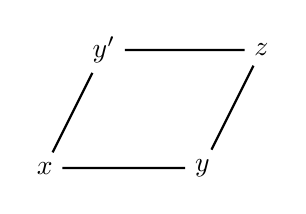
\begin{tikzpicture}
    \node (bl) at (0,0) {$x$};
    \node (br) at (2,0) {$y$};
    \node (tl) at (0.75,1.5) {$y'$};
    \node (tr) at (2.75,1.5) {$z$};
    \draw[thick] (bl) to (tl) to (tr) to (br) to (bl);
  \end{tikzpicture}
\] So
\[\mbox{$xRSz$ iff $x-y$ is in $R$ and $y-z$ is in $S$ for some $y$,}\]
while
\[\mbox{$xSRz$ iff $x-y'$ is in $S$ and $y'-z$ is in $R$ for some $y'$.}\]
but the picture shows these are equivalent!

If we start with a vector space over the reals, complexes or
quaternions, the lattice we get this way is exactly the same as the
lattice we get starting from the corresponding projective space, so
Desargues' theorem in this case is just a corollary of the fact that
Desargues' theorem holds for all linear lattices.

On the other hand, since the lattice associated to the octonionic
projective plane does \emph{not} satisfy Desargues' theorem, it's not a
linear lattice. Maybe someday I'll use these ideas to understand what's
weird about octonionic quantum mechanics.

But another cool thing is that Mark Haiman has cooked up a set of
deduction rules that let you derive precisely all the implications that
hold in all linear lattices. Even better, there's a way to draw pictures
of these deduction rules, which makes them look a bit like tricks for
rewiring electrical circuits! You can learn about this in the above
paper, or Haiman's original paper:

\begin{enumerate}
\def\labelenumi{\arabic{enumi})}
\setcounter{enumi}{3}
\tightlist
\item
  Mark Haiman, ``Proof theory for linear lattices'', \emph{Adv. Math.}
  \textbf{58} (1985), 209--242.
\end{enumerate}

or this followup:

\begin{enumerate}
\def\labelenumi{\arabic{enumi})}
\setcounter{enumi}{4}
\tightlist
\item
  D. Finberg, M. Mainetti and G.-C. Rota, ``The logic of commuting
  equivalence relations'', in \emph{Logic and Algebra}, eds.~A. Ursini
  and P. Agliano, Lecture Notes in Pure and Applied Mathematics,
  vol.~\textbf{180}, Decker, New York 1996.
\end{enumerate}

To finish up, let me add that there are lots of linear lattices. For
example, we can try generalizing the above trick from vector spaces to
groups! Given any group \(G\), each subgroup \(H\) determines an
equivalence relation on \(G\), which by abuse of language I'll call
\(H\), such that \(xHy\) iff \(xy^{-1}\) is in \(H\). If \(G\) is
abelian all these equivalence relations commute, so the lattice of
subgroups of \(G\) becomes a linear lattice. If \(G\) is nonabelian this
trick breaks down unless we use \emph{normal} subgroups.

I should also add that nobody has figured out whether the collection of
linear lattices can be characterized by identities\ldots{} though they
satisfy lots of interesting identities, like the famous ``modular law'':
\[x \operatorname{and} (y \operatorname{or} (x \operatorname{and} z)) = (x \operatorname{and} y) \operatorname{or} (x \operatorname{and} z)\]
This is one reason Haiman's proof theory is interesting.

Now, on to some category theory!

Michael Mueger has written some excellent papers on the relation between
quantum field theory, category theory, and topology:

\begin{enumerate}
\def\labelenumi{\arabic{enumi})}
\setcounter{enumi}{5}
\tightlist
\item
  Michael Mueger, ``Conformal field theory and Doplicher-Roberts
  reconstruction'', available at
  \href{https://arxiv.org/abs/math-ph/0008027}{\texttt{math-ph/0008027}}.
\end{enumerate}

``From subfactors to categories and topology I: Frobenius algebras in
and Morita equivalence of tensor categories'', available at
\href{https://arxiv.org/abs/math.CT/0111204}{\texttt{math.CT/0111204}}.

``From subfactors to categories and topology II: The quantum double of
tensor catgories and subfactors'', available at
\href{https://arxiv.org/abs/math.CT/0111205}{\texttt{math.CT/0111205}}.

I can't possibly do justice to these, but I'd like to discuss a very
pretty idea from his paper on Frobenius algebras. This will give me a
good chance to continue some themes from my earlier issues on
\(n\)-categories and homotopy theory.

In \protect\hyperlink{week83}{``Week 83''} I talked about adjoint
functors, and more generally, adjunctions in any \(2\)-category. If you
don't understand this stuff, you're a goner now, but let me just remind
you of the definitions. Suppose \(a\) and \(b\) are objects in a
\(2\)-category. Then we say the morphism \[L\colon a \to b\] is a ``left
adjoint'' of the morphism \[R\colon b \to a\] (and \(R\) is a ``right
adjoint'' of \(L\)) if there are \(2\)-morphisms called the ``unit''
\[i: 1a \Rightarrow LR\] and ``counit'' \[e: RL \Rightarrow 1b\]
satisfying the ``triangle equations'', which say that these vertical
composites are both identity \(2\)-morphisms:
\[L = 1_aL \xRightarrow{i\cdot1_L} LRL \xRightarrow{1_L\cdot e} L1_a = L\]
and
\[R = R1_b \xRightarrow{1_R\cdot i} RLR \xRightarrow{e\cdot1_R} 1_bR = R\]
where \(\cdot\) denotes horizontal composition. The whole setup
\((a,b,L,R,e,i)\) is then called an ``adjunction''.

There are some important variations on this theme. For example, if \(e\)
and \(i\) are invertible, but we drop the triangle equations, we call
the setup an ``equivalence''. It's morally correct to consider two
objects \(a\) and \(b\) in a \(2\)-category ``the same for all practical
purposes'' if they take part in an equivalence. A special case is when
they are \emph{equal} --- since then we can take \(L,R,e,i\) to be
identities. Another special case is when they are \emph{isomorphic} -
since then we can take \(L\) to be an isomorphism, \(R\) its inverse,
and \(e\) and \(i\) to be identities. But in general we only need \(L\)
and \(R\) to be isomorphisms ``up to 2-isomorphism''.

So, the notion of equivalence is better than equality, because it
follows the fundamental principle of \(n\)-category theory: everything
is only true up to something!

If \(e\) and \(i\) are invertible and we \emph{keep} the triangle
equations, we call the setup an ``adjoint equivalence''. In other words,
an adjoint equivalence is an adjunction that is also an equivalence.
This is a bit better than an equivalence. Recently on the category
theory mailing list Paul Levy asked exactly how much better. The first
answer is: not much, because given any equivalence we can cook up an
adjoint equivalence by just fiddling with either the unit or counit in a
standard way, using only the material at hand: \((a,b,R,L,i,e)\). I
leave this as a fun exercise\ldots.

But the second answer, which James Dolan and I worked out this Friday,
goes like this:

First, consider the ``Platonic idea of an equivalence''. By this, I mean
the \(2\)-category \(\mathsf{Equiv}\) which is freely generated by
objects \(a\) and \(b\), morphisms \(L\colon a \to b\) and
\(R\colon b \to a\), and isomorphisms \(i\colon 1_b \Rightarrow RL\) and
\(e\colon LR \Rightarrow 1_a\). Why do I call this the ``Platonic idea
of an equivalence''? Well, any equivalence in any \(2\)-category
\(\mathcal{C}\) is just the same as a 2-functor
\[F\colon \mathsf{Equiv} \to \mathcal{C}\] The functor \(F\) turns the
``abstract'' equivalence in \(\mathsf{Equiv}\) into a ``concrete''
equivalence in \(\mathcal{C}\)! This is reminiscent of Plato's theory of
ideas and how they get manifested in concrete situations. We can think
of \(\mathsf{Equiv}\) as the unadorned idea of an adjunction without any
contamination by accidental extra features.

I should add that James, less of an intellectual snob than I, calls
\(\mathsf{Equiv}\) the ``walking equivalence''. After all, if someone
has really big bushy eyebrows, so that when you see him walking down the
street you first notice his eyebrows and only later realize there's a
person attached, you call him a ``walking pair of eyebrows''. The person
is basically just the life support system for the eyebrows! Similarly,
in \(\mathsf{Equiv}\) we have a \(2\)-category which is just the life
support system for an adjunction: no more and no less.

Anyway, the walking equivalence is a weak \(2\)-groupoid: a
\(2\)-category where every \(2\)-morphism is invertible and every
morphism is invertible up to 2-isomorphism. Weak \(2\)-groupoids are
secretly the same thing as homotopy 2-types: roughly speaking,
topological spaces whose homotopy groups vanish above dimension 2. And
there's a pretty easy way to turn a weak \(2\)-groupoid into a homotopy
2-type. First you turn it into a simplicial set, called its ``nerve'',
and then you take the geometric realization of that.

Eh? Well, I talked about geometric realization in part E of
\protect\hyperlink{week116}{``Week 116''}, and I talked about the nerve
of a \(1\)-category in part J of \protect\hyperlink{week117}{``Week
117''}, so the only thing I need to do is say a bit about the nerve of a
\(2\)-category. This is a simplicial set where the 0-simplices
correspond to objects: \[x\] the \(1\)-simplices correspond to
morphisms: \[x\xrightarrow{F}Y\] the \(2\)-simplices correspond to
\(2\)-morphisms: \[
  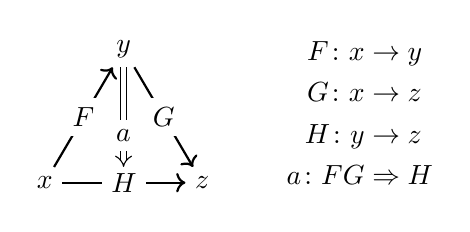
\begin{tikzpicture}
    \node (x) at (0,0) {$x$};
    \node (y) at (1,1.7) {$y$};
    \node (z) at (2,0) {$z$};
    \draw[thick,->] (x) to node[fill=white]{$F$} (y);
    \draw[thick,->] (x) to node[fill=white]{$H$} (z);
    \draw[thick,->] (y) to node[fill=white]{$G$} (z);
    \draw[double,double equal sign distance,-implies] (y) to (1,0.2);
    \node[fill=white] at (1,0.6) {$a$};
    \node at (4,0.85) {$
      \begin{aligned}
        F\colon x&\to y
      \\G\colon x&\to z
      \\H\colon y&\to z
      \\a\colon FG&\Rightarrow H
      \end{aligned}
    $};
  \end{tikzpicture}
\] and the higher-dimensional simplices correspond to equations,
``equations between equations'', and so on.

Anyway, if you use this trick to turn the walking equivalence into a
space, what space do you get?

The 2-sphere!

It's pretty easy to see\ldots{} I'd draw it for you on paper if I could,
but you'll have to do it yourself. It helps if you have a globe:

\begin{itemize}
\tightlist
\item
  \(a\) is the North Pole,
\item
  \(b\) is the South Pole,
\item
  \(L\colon a \to b\) is the Greenwich Meridian running from north to
  south,
\item
  \(R\colon b \to a\) is the International Date Line running from south
  to north,
\item
  \(i\colon 1_a \Rightarrow LR\) is the Eastern Hemisphere, and
\item
  \(e\colon RL \Rightarrow 1_b\) is the Western Hemisphere!
\end{itemize}

(More precisely, we just get the 2-sphere up to homotopy equivalence:
there is a whole bunch of higher-dimensional flab which I'm ignoring
here. But that's okay, since we're doing homotopy theory.)

We can also play this game for the ``walking adjoint equivalence'',
\(\mathsf{AdEquiv}\). This is just like the walking equivalence, except
we put in extra relations: the triangle equations. How does this affect
the space we get?

It's very beautiful: the extra equations fill in the 2-sphere to give us
a 3-ball! (At least up to homotopy equivalence.)

Now, the 3-ball is contractible, so as a homotopy type it's really the
same as a point. And a point is exactly the space we'd get from playing
the same game starting with the ``walking object'': the \(2\)-category
with one object, its identity morphism, and the identity \(2\)-morphism
of that.

To the eyes of a homotopy theorist, a point and 3-ball are the same, but
the 2-sphere is not. Similarly, to the eyes of an \(n\)-category
theorist, the walking object and the walking adjoint equivalence are
``the same'', but the walking equivalence is not!

We could make this very precise with a suitable notion of ``sameness''
for \(2\)-categories. But instead, let's jump straight to the punchline:
having an adjoint equivalence in a \(2\)-category is ``the same'' as
having an object\ldots. but having an equivalence is not!

There's even more fun to be had here. Since every adjoint equivalence is
an equivalence, there's a 2-functor
\[I\colon \mathsf{Equiv} \to \mathsf{AdEquiv}\] But I also said every
equivalence can be massaged to obtain an adjoint equivalence! In fact, I
said it could be done in two equally good ways. Either of these gives a
2-functor \[P\colon \mathsf{AdEquiv} \to \mathsf{Equiv}\] Now, we can
ask what these become when we turn them into maps between spaces\ldots.

It turns out that \(I\) is just the inclusion of the 2-sphere into the
3-ball, while \(P\) is the map that squashes the 3-ball down to either
the eastern or western hemisphere of the sphere!

By the way, it is irresistible to predict generalizations to higher
dimensions. For any \(n\), we will have weak \(n\)-groupoids called
\(\mathsf{Equiv}\), the ``walking \(n\)-equivalence'', and
\(\mathsf{AdEquiv}\), the ``walking adjoint n-equivalence''. The
geometric realization of the nerve of \(\mathsf{Equiv}\) will be
homotopy equivalent to the \(n\)-sphere, while that of
\(\mathsf{AdEquiv}\) will be homotopy equivalent to the \((n+1)\)-ball.

(Note that for \(n = 1\), \(\mathsf{Equiv}\) will be the category with
objects \(a\) and \(b\) and isomorphisms \(L\colon a \to b\),
\(R\colon b \to a\). In \(\mathsf{AdEquiv}\), there will be extra
relations saying that \(R\) is the inverse of \(L\). In this sense, it
is really an adjoint equivalence rather than an equivalence which is the
proper generalization of an isomorphism!)

Okay. Believe it or not, I still haven't gotten to the stuff Michael
Mueger was talking about! I got distracted. I talked about the walking
equivalence and the walking adjoint equivalence, but next week, I'll
talk about the walking adjunction\ldots{} and finally the walking
``biadjunction'', which is where Mueger comes in.

\begin{center}\rule{0.5\linewidth}{0.5pt}\end{center}

Postscript --- Keith Harbaugh writes:

\begin{quote}
Since you're back on Desargues again, just thought I'd mention (in case
you haven't already noticed this) that if you look up Desargues in
``Categories, Allegories'' by Freyd and Scedrov, you'll find that they
(probably really Freyd) have a neat proof of Desargues in the context of
their ``allegories'' (\(2\)-categories with structure modeled on the
bicategory of relations).
\end{quote}

Linus Kramer writes:

\begin{quote}
I'd like to comment on the interesting paper by Thomas Püttmann and A.
Rigas, Isometric actions on the projective planes and embedded
generators of homotopy groups, available at

\texttt{http://www.ruhr-uni-bochum.de/mathematik8/puttmann/index.html}

which is mentioned in Baez' article.

As Baez writes, the authors construct an embedding of the 11-sphere into
the Cayley plane \(\mathbb{OP}^2\). This embedding is closely related to
a polarity (a polarity of a projective plane is an involution which maps
points to lines and vice versa, and which preserves incidence).

The simplest example is the elliptic polarity over the reals. Take the
standard inner product on R\^{}3 and consider the map which sends a
subspace to its perp. Now the points of the real projective plane are
the \(1\)-dimensional subspaces, and the lines are the \(2\)-dimensional
subspaces. It is fairly easy to see that this map `take the perp' is a
polarity.

Now there is also a different polarity: take a Minkowski-like metric on
\(\mathbb{R}^3\), (\(++-\)). In exactly the same way as above, one
obtains a polarity, the hyperbolic polarity of the real projective
plane. This polarity has absolute elements, i.e.~elements which are
incident with their image under the polarity: this happens with all
1-dim. subspaces which are `light-like', i.e.~on which the metric
vanishes. The set of all absolute points in \(\mathbb{RP}^2\) is a
1-sphere.

One can prove that up to automorphisms, these two are the only
polarities for the real projective plane \(\mathbb{RP}^2\). Notice the
associated motion groups \(\mathrm{SO}_3(\mathbb{R})\) and
\(\mathrm{SO}_{2,1}(\mathbb{R})\) (the motion group consists of all
collineations which commute with the polarity).

Similar polarities can be defined for the complex, the quaternionic and
the octonionic projective planes. One obtains elliptic (no absolute
points) and hyperbolic (many absolute points) polarities. In the second
case, the set of absolute points are spheres of dimensions 3,7,15,
respectively.

But for these latter projective planes, there are more polarities! There
is one more polarity (called `planar polarity' by some authors) which
has a different kind of absolute points. For these polarities, one
obtains spheres of dimension 2,5,11, respectively for the absolute
points.

These semi-classical embeddings were (re)discovered by the authors. The
corresponding motion groups are by the way simple; they are
\(SO_{3,1}(\mathbb{R})\), \(SU_{3,1}(\mathbb{C})\) and
\(SU_{3,1}(\mathbb{H})=\mathrm{Sp}_{3,1}\). If one looks only for
isometric motions (as the authors do) (i.e.~motions which centralize at
the same time the elliptic polarity) one obtains the compact groups
mentioned in the article.

Of course, the main point of the authors is that they obtain generators
of the 11th homotopy group, and this is certainly a new and beautiful
result. I just wanted to mention some related `classical' results from
projective geometry.

A good source here is, as always, Salzmann et al., Compact Projective
Planes, de Gruyter 1995, p.~127.

Regards, Linus Kramer
\end{quote}



\hypertarget{week174}{%
\section{November 28, 2001}\label{week174}}

Groups are how mathematicians and physicists talk about symmetry, and
Lie groups are how they talk about \emph{continuously varying}
symmetries, like rotations, translations and the like. Sophus Lie helped
start the subject of Lie groups in the late 1800s, and it's been in
constant growth ever since. I spend lots of time studying it, and I
probably will all my life --- there's a lot to learn! To really
understand it, it helps to know the history. And for that, this is the
book to read:

\begin{enumerate}
\def\labelenumi{\arabic{enumi})}
\tightlist
\item
  Thomas Hawkins, \emph{The Emergence of the Theory of Lie Groups: an
  Essay in the History of Mathematics, 1869--1926}, Springer, New York,
  2000.
\end{enumerate}

You have to know your Lie groups pretty well to enjoy this book, but if
you do, you'll find it's full of interesting facts. For example: folks
often complain about Wilhelm Killing's original classification of simple
Lie algebras --- it wasn't rigorous, he made some mistakes, and so on.
Elie Cartan came along later and cleaned it up, and many people applaud
Cartan's work and sneer at poor old Killing, even though he was the one
who came up with the original ideas. But in this book, it becomes clear
that Killing was pretty much \emph{pushed} into publishing his ideas in
a half-baked state by mathematicians who were dying to know his results!
Now I feel even more sorry for him.

There's also a lot of interesting stuff about Hermann Weyl's approach to
representation theory via tensors and Young diagrams, and why he liked
it better than Cartan's approach via roots and weights. Basically, Weyl
liked his approach because it stuck closer to Felix Klein's original
``Erlanger program'' --- a program for understanding geometry via
symmetry groups. But it's interesting to see how Weyl studied and
respected Cartan's approach, and tried to bridge the gap between the
two.

Okay\ldots{} so much for gossip! Now I'm going to dive in and pick up
right where I left off in my discussion of the ideas behind this paper:

\begin{enumerate}
\def\labelenumi{\arabic{enumi})}
\setcounter{enumi}{1}
\tightlist
\item
  Michael Mueger, ``From subfactors to categories and topology I:
  Frobenius algebras in and Morita equivalence of tensor categories'',
  available at
  \href{https://arxiv.org/abs/math.CT/0111204}{\texttt{math.CT/0111204}}.
\end{enumerate}

My ultimate goal is to take you to an elegant understanding of Frobenius
algebras by means of a \(2\)-category called the ``walking ambidextrous
adjunction'', but first I'll play around a bit with a simpler but more
famous \(2\)-category called the ``walking adjunction''. This may sound
scary, but if you can stick with it, you'll see that I'm really just
using these \(2\)-categories to describe fun games that you can play
with certain \(2\)-dimensional pictures. Even if you don't read the
words, please stare at the pictures --- I spend my Thanksgiving weekend
drawing them, and I don't want that work to go to waste!

Category theorists love to talk about adjoint functors, but
\(2\)-category theorists know that these are just a special example of
an ``adjunction''. An adjunction is something that makes sense in any
\(2\)-category; if we take the \(2\)-category to be \(\mathsf{Cat}\) we
get adjoint functors. There are lots of other nice examples that make
this generalization worthwhile. For example, in
\protect\hyperlink{week83}{``Week 83''} I explained how a pair of dual
vector spaces is also an example of an adjunction.

To study adjunctions, it suffices to study the ``walking adjunction''.
This is a little \(2\)-category containing exactly the stuff any
adjunction in any \(2\)-category must have: not a jot more, not a tiddle
less! It was first studied by Schanuel and Street:

\begin{enumerate}
\def\labelenumi{\arabic{enumi})}
\setcounter{enumi}{2}
\tightlist
\item
  Stephen Schanuel and Ross Street, ``The free adjunction'', \emph{Cah.
  Top. Geom. Diff.} \textbf{27} (1986), 81--83.
\end{enumerate}

In a bit more detail, the walking adjunction is the \(2\)-category
freely generated by two objects: \[\mbox{$a$ and $b$,}\] two morphisms:
\[\mbox{$L\colon a \to b$ and $R\colon b \to a$,}\] and two
\(2\)-morphisms, called the ``unit'' and ``counit'':
\[\mbox{$i\colon 1_a \Rightarrow LR$ and $e\colon RL \Rightarrow 1_b$}\]
satisfying two relations, called the ``triangle equations''.

I wrote down these equations already last week, but let me do it again
using ``string diagrams'', as explained in
\protect\hyperlink{week79}{``Week 79''} and
\protect\hyperlink{week92}{``Week 92''}. In a \(2\)-categorical string
diagram, objects are denoted by 2d regions in the plane, morphisms are
denoted by 1d edges, and \(2\)-morphisms are denoted by 0d points. If
the dimensions look sort of upside-down, you're right --- that's exactly
the point!

Instead of explaining the whole theory, I'll just plunge in with the
example at hand. The unit \(i\) looks like this: \[
  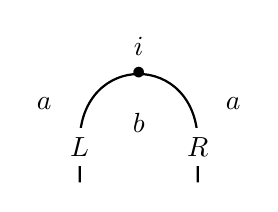
\begin{tikzpicture}[yscale=-1]
    \begin{knot}
      \strand[thick] (0,0)
      to (0,-0.5)
      to [out=down,in=down,looseness=2] (1.5,-0.5)
      to (1.5,0);
    \end{knot}
    \node[fill=white] at (0,-0.45) {$L$};
    \node[fill=white] at (1.5,-0.45) {$R$};
    \node[label={[label distance=-1mm]above:{$i$}}] at (0.75,-1.39) {$\bullet$};
    \node at (0.75,-0.75) {$b$};
    \node at (-0.45,-1) {$a$};
    \node at (1.95,-1) {$a$};
  \end{tikzpicture}
\] while the counit \(e\) looks like this: \[
  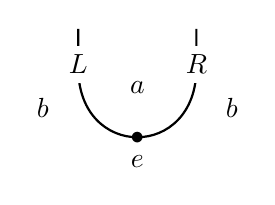
\begin{tikzpicture}
    \begin{knot}
      \strand[thick] (0,0)
      to (0,-0.5)
      to [out=down,in=down,looseness=2] (1.5,-0.5)
      to (1.5,0);
    \end{knot}
    \node[fill=white] at (0,-0.45) {$L$};
    \node[fill=white] at (1.5,-0.45) {$R$};
    \node[label={[label distance=-1mm]below:{$e$}}] at (0.75,-1.39) {$\bullet$};
    \node at (0.75,-0.75) {$a$};
    \node at (-0.45,-1) {$b$};
    \node at (1.95,-1) {$b$};
  \end{tikzpicture}
\] Note that as you cross a line labelled ``\(L\)'' from left to right,
you go from region \(a\) to region \(b\), which is our way of saying
that \(L\colon a\to b\). Similarly, as you cross a line labelled
``\(R\)'' from left to right, you go from region \(b\) to region \(a\),
since \(R\colon b\to a\).

In terms of string diagrams, the triangle equations just say that we can
straighten out a zig-zag: \[
  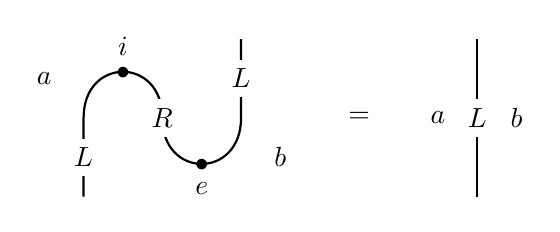
\begin{tikzpicture}
    \begin{scope}
      \begin{knot}
        \strand[thick] (0,0)
        to (0,1)
        to [out=up,in=up,looseness=2] (1,1)
        to [out=down,in=down,looseness=2] (2,1)
        to (2,2);
      \end{knot}
      \node at (-0.5,1.5) {$a$};
      \node[fill=white] at (0,0.5) {$L$};
      \node[label={[label distance=-1mm]above:{$i$}}] at (0.5,1.57) {$\bullet$};
      \node[fill=white] at (1,1) {$R$};
      \node[label={[label distance=-1mm]below:{$e$}}] at (1.5,0.4) {$\bullet$};
      \node[fill=white] at (2,1.5) {$L$};
      \node at (2.5,0.5) {$b$};
    \end{scope}
    \node at (3.5,1) {$=$};
    \begin{scope}[shift={(5,2)}]
      \node at (-0.5,-1) {$a$};
      \draw[thick] (0,0) to node[fill=white]{$L$} (0,-2);
      \node at (0.5,-1) {$b$};
    \end{scope}
  \end{tikzpicture}
\] or a zag-zig: \[
  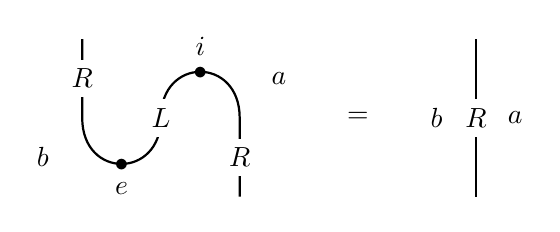
\begin{tikzpicture}
    \begin{scope}[xscale=-1,shift={(-2,0)}]
      \begin{knot}
        \strand[thick] (0,0)
        to (0,1)
        to [out=up,in=up,looseness=2] (1,1)
        to [out=down,in=down,looseness=2] (2,1)
        to (2,2);
      \end{knot}
      \node at (-0.5,1.5) {$a$};
      \node[fill=white] at (0,0.5) {$R$};
      \node[label={[label distance=-1mm]above:{$i$}}] at (0.5,1.57) {$\bullet$};
      \node[fill=white] at (1,1) {$L$};
      \node[label={[label distance=-1mm]below:{$e$}}] at (1.5,0.4) {$\bullet$};
      \node[fill=white] at (2,1.5) {$R$};
      \node at (2.5,0.5) {$b$};
    \end{scope}
    \node at (3.5,1) {$=$};
    \begin{scope}[shift={(5,2)}]
      \node at (-0.5,-1) {$b$};
      \draw[thick] (0,0) to node[fill=white]{$R$} (0,-2);
      \node at (0.5,-1) {$a$};
    \end{scope}
  \end{tikzpicture}
\] We can build any \(2\)-morphism in the walking adjunction by
vertically and horizontally composing units and counits, which
corresponds to sticking together string diagrams in a vertical or
horizontal way. Thus, a typical \(2\)-morphism looks like this: \[
  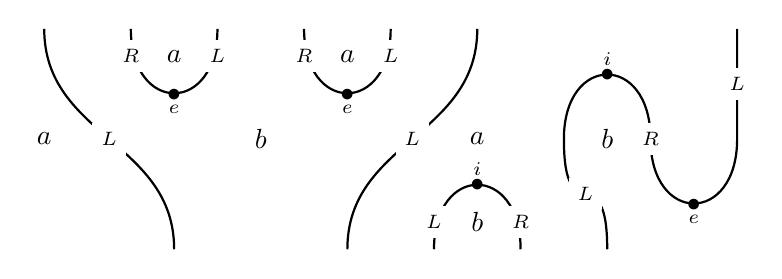
\begin{tikzpicture}[xscale=1.1,yscale=1.4]
    \begin{knot}
      \strand[thick] (-0.5,0)
        to [out=up,in=down] (-2,2);
      \strand[thick] (-1,2)
        to [out=down,in=down,looseness=2] (0,2);
      \strand[thick] (1,2)
        to [out=down,in=down,looseness=2] (2,2);
      \strand[thick] (1.5,0)
        to [out=up,in=down] (3,2);
      \strand[thick] (2.5,0)
        to [out=up,in=up,looseness=2] (3.5,0);
      \strand[thick] (4.5,0)
        to [out=up,in=down,looseness=2] (4,1)
        to [out=up,in=up,looseness=2] (5,1)
        to [out=down,in=down,looseness=2] (6,1)
        to (6,2);
    \end{knot}
    \node at (-2,1) {$a$};
    \node at (-0.5,1.75) {$a$};
    \node at (1.5,1.75) {$a$};
    \node at (0.5,1) {$b$};
    \node at (3,1) {$a$};
    \node at (3,0.25) {$b$};
    \node at (4.5,1) {$b$};
    %
    \node[fill=white] at (-1.25,1) {\scriptsize$L$};
    \node[fill=white] at (-1,1.75) {\scriptsize$R$};
    \node[fill=white] at (0,1.75) {\scriptsize$L$};
    \node[fill=white] at (1,1.75) {\scriptsize$R$};
    \node[fill=white] at (2,1.75) {\scriptsize$L$};
    \node[fill=white] at (2.25,1) {\scriptsize$L$};
    \node[fill=white] at (2.5,0.25) {\scriptsize$L$};
    \node[fill=white] at (3.5,0.25) {\scriptsize$R$};
    \node[fill=white] at (4.25,0.5) {\scriptsize$L$};
    \node[fill=white] at (5,1) {\scriptsize$R$};
    \node[fill=white] at (6,1.5) {\scriptsize$L$};
    %
    \node[label={[label distance=-2mm]below:{\scriptsize$e$}}] at (-0.5,1.4) {$\bullet$};
    \node[label={[label distance=-2mm]below:{\scriptsize$e$}}] at (1.5,1.4) {$\bullet$};
    \node[label={[label distance=-2mm]above:{\scriptsize$i$}}] at (3,0.58) {$\bullet$};
    \node[label={[label distance=-2mm]below:{\scriptsize$e$}}] at (5.5,0.4) {$\bullet$};
    \node[label={[label distance=-2mm]above:{\scriptsize$i$}}] at (4.5,1.58) {$\bullet$};
  \end{tikzpicture}
\] By the triangle equations, we could straighten out the zig-zag
without changing the \(2\)-morphism.

As you may know, the word ``anaranjado'' means ``orange'' in Spanish ---
there was no word in English for ``orange'' before people in England
started importing oranges from Spain. And this is a nice mnemonic,
because if we take the above picture and paint the regions labelled
``\(a\)'' orange, and paint the regions labelled ``\(b\)'' black, the
above picture has a roughly tiger-striped appearance. In fact, these
tiger stripes tell you everything you need to know about the
\(2\)-morphism! For example, starting from just this: \[
  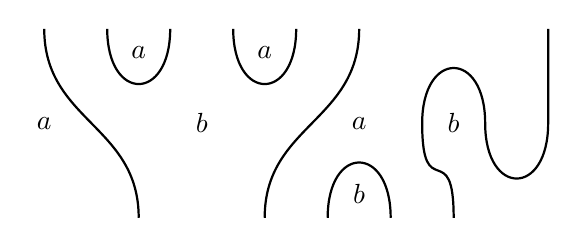
\begin{tikzpicture}[xscale=0.8,yscale=1.2]
    \begin{knot}
      \strand[thick] (-0.5,0)
        to [out=up,in=down] (-2,2);
      \strand[thick] (-1,2)
        to [out=down,in=down,looseness=2] (0,2);
      \strand[thick] (1,2)
        to [out=down,in=down,looseness=2] (2,2);
      \strand[thick] (1.5,0)
        to [out=up,in=down] (3,2);
      \strand[thick] (2.5,0)
        to [out=up,in=up,looseness=2] (3.5,0);
      \strand[thick] (4.5,0)
        to [out=up,in=down,looseness=2] (4,1)
        to [out=up,in=up,looseness=2] (5,1)
        to [out=down,in=down,looseness=2] (6,1)
        to (6,2);
    \end{knot}
    \node at (-2,1) {$a$};
    \node at (-0.5,1.75) {$a$};
    \node at (1.5,1.75) {$a$};
    \node at (0.5,1) {$b$};
    \node at (3,1) {$a$};
    \node at (3,0.25) {$b$};
    \node at (4.5,1) {$b$};
  \end{tikzpicture}
\] you can figure out where everything else should go.

By the way, note that orange stripes can disappear as we go down the
page, and they can split, but they can't appear or merge. Black stripes
can appear or merge, but they can't disappear or split. As a result,
there can never be any orange or black \emph{spots}. We'll change these
rules later, when we talk about the walking ``ambidextrous adjunction''.

Okay, so we've got this \(2\)-category, the walking adjunction: let's
call it \(\mathsf{Ad}\) for short. It's pretty simple. How can we
understand it better?

Well, for any two objects \(a\) and \(b\) in a \(2\)-category we get a
``hom-category'' \(\operatorname{Hom}(a,b)\), whose objects are the
morphisms from \(a\) to \(b\), and whose morphisms are the
\(2\)-morphisms between those. If we work out these hom-categories in
\(\mathsf{Ad}\), we get some cool stuff.

First let's look at the hom-category \(\operatorname{Hom}(a,a)\). In
this category, the objects are \[1_a, LR, LRLR, LRLRLR, \ldots\] and all
the morphisms are built by sticking these two basic generators together
vertically or horizontally: \[
  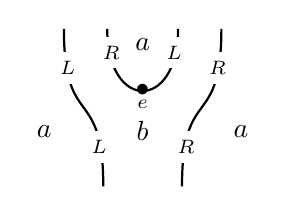
\begin{tikzpicture}[yscale=2]
    \begin{knot}
      \strand[thick] (-0.5,0)
        to [out=up,in=down,looseness=1.5] (-1,1);
      \strand[thick] (-0.45,1)
        to [out=down,in=down,looseness=1.5] (0.45,1);
      \strand[thick] (0.5,0)
        to [out=up,in=down,looseness=1.5] (1,1);
    \end{knot}
    %
    \node at (-1.25,0.35) {$a$};
    \node at (0,0.35) {$b$};
    \node at (0,0.9) {$a$};
    \node at (1.25,0.35) {$a$};
    %
    \node[fill=white] at (-0.55,0.25) {\scriptsize$L$};
    \node[fill=white] at (-0.95,0.75) {\scriptsize$L$};
    \node[fill=white] at (-0.4,0.85) {\scriptsize$R$};
    \node[fill=white] at (0.4,0.85) {\scriptsize$L$};
    \node[fill=white] at (0.55,0.25) {\scriptsize$R$};
    \node[fill=white] at (0.95,0.75) {\scriptsize$R$};
    \node[label={[label distance=-2mm]below:{\scriptsize$e$}}] at (0,0.61) {$\bullet$};
  \end{tikzpicture}
\] and \[
  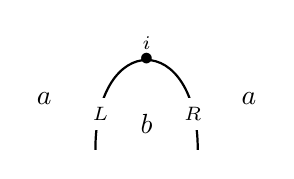
\begin{tikzpicture}[scale=1.3]
    \begin{knot}
      \strand[thick] (-0.5,0)
        to [out=up,in=up,looseness=3] (0.5,0);
    \end{knot}
    \node at (-1,0.5) {$a$};
    \node at (0,0.25) {$b$};
    \node at (1,0.5) {$a$};
    \node[fill=white] at (-0.45,0.35) {\scriptsize$L$};
    \node[fill=white] at (0.45,0.35) {\scriptsize$R$};
    \node[label={[label distance=-2mm]above:{\scriptsize$i$}}] at (0,0.88) {$\bullet$};
  \end{tikzpicture}
\] In tiger language, we're talking about pictures of black stripes on
an orange background. The two basic generators are the merging of two
black stripes and the appearance of a black stripe.

If you read \protect\hyperlink{week89}{``Week 89''}, you'll know another
way to describe this! Our ability to stick together pictures vertically
and horizontally makes \(\operatorname{Hom}(a,a)\) into a ``monoidal
category''. \(LR\) is a ``monoid object'', with merging of two black
stripes being ``multiplication'', and the appearance of a black stripe
being the ``multiplicative identity''. Being a ``monoid object'' simply
means that these operations satisfy the left unit law: \[
  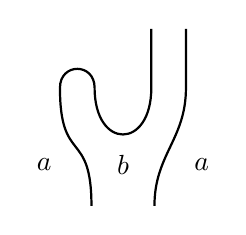
\begin{tikzpicture}[xscale=0.8,yscale=1.5]
    \begin{knot}
      \strand[thick] (-0.5,0)
        to [out=up,in=down,looseness=1.5] (-1,1)
        to [out=up,in=up,looseness=1] (-0.45,1)
        to [out=down,in=down,looseness=1.5] (0.45,1)
        to (0.45,1.5);
      \strand[thick] (0.5,0)
        to [out=up,in=down,looseness=1] (1,1)
        to (1,1.5);
    \end{knot}
    %
    \node at (-1.25,0.35) {$a$};
    \node at (0,0.35) {$b$};
    \node at (1.25,0.35) {$a$};
  \end{tikzpicture}
  \quad
  \raisebox{3em}{$=$}
  \quad
  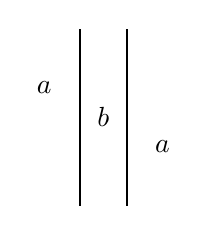
\begin{tikzpicture}[yscale=1.5]
    \draw[thick] (-0.3,0) to (-0.3,1.5);
    \draw[thick] (0.3,0) to (0.3,1.5);
    %
    \node at (-0.75,1) {$a$};
    \node at (0,0.75) {$b$};
    \node at (0.75,0.5) {$a$};
  \end{tikzpicture}
\] and its mirror image, called the right unit law, together with the
associative law: \[
  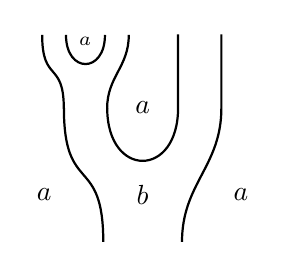
\begin{tikzpicture}[xscale=1,yscale=1.7]
    \begin{knot}
      \strand[thick] (-0.5,0)
        to [out=up,in=down,looseness=1.5] (-1,1);
      \strand[thick] (-0.45,1)
        to [out=down,in=down,looseness=1.5] (0.45,1)
        to (0.45,1.55);
      \strand[thick] (0.5,0)
        to [out=up,in=down,looseness=1] (1,1)
        to (1,1.55);
    \end{knot}
    \begin{scope}[scale=0.55,shift={(-1.32,1.81)}]
      \begin{knot}
        \strand[thick] (-0.5,0)
          to [out=up,in=down,looseness=1.5] (-1,1);
        \strand[thick] (-0.45,1)
          to [out=down,in=down,looseness=1.5] (0.45,1);
        \strand[thick] (0.5,0)
          to [out=up,in=down,looseness=1] (1,1);
      \end{knot}
    \end{scope}
    %
    \node at (-1.25,0.35) {$a$};
    \node at (0,0.35) {$b$};
    \node at (1.25,0.35) {$a$};
    \node at (-0.73,1.5) {\scriptsize$a$};
    \node at (0,1) {$a$};
  \end{tikzpicture}
  \quad
  \raisebox{4em}{$=$}
  \quad
  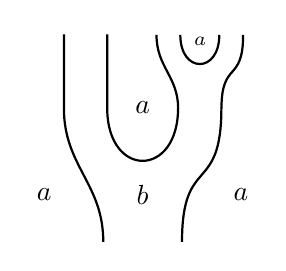
\begin{tikzpicture}[xscale=-1,yscale=1.7]
    \begin{knot}
      \strand[thick] (-0.5,0)
        to [out=up,in=down,looseness=1.5] (-1,1);
      \strand[thick] (-0.45,1)
        to [out=down,in=down,looseness=1.5] (0.45,1)
        to (0.45,1.55);
      \strand[thick] (0.5,0)
        to [out=up,in=down,looseness=1] (1,1)
        to (1,1.55);
    \end{knot}
    \begin{scope}[scale=0.55,shift={(-1.32,1.81)}]
      \begin{knot}
        \strand[thick] (-0.5,0)
          to [out=up,in=down,looseness=1.5] (-1,1);
        \strand[thick] (-0.45,1)
          to [out=down,in=down,looseness=1.5] (0.45,1);
        \strand[thick] (0.5,0)
          to [out=up,in=down,looseness=1] (1,1);
      \end{knot}
    \end{scope}
    %
    \node at (-1.25,0.35) {$a$};
    \node at (0,0.35) {$b$};
    \node at (1.25,0.35) {$a$};
    \node at (-0.73,1.5) {\scriptsize$a$};
    \node at (0,1) {$a$};
  \end{tikzpicture}
\] There aren't any other laws, so \(\operatorname{Hom}(a,a)\) is the
``free monoidal category on a monoid object'', or if you prefer, the
``walking monoid''!

I touched upon the immense consequences of this fact for algebraic
topology in \protect\hyperlink{week117}{``Week 117''} and
\protect\hyperlink{week118}{``Week 118''}. They mainly rely on another
way of thinking about \(\operatorname{Hom}(a,a)\): it's the category of
order-preserving maps between finite ordinals!

For example, these black tiger stripes on an orange background: \[
  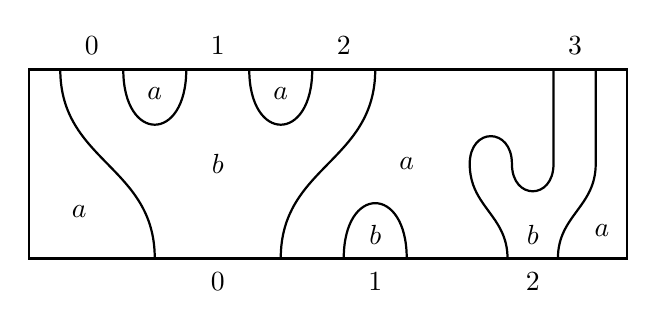
\begin{tikzpicture}[xscale=0.8,yscale=1.2]
    \begin{knot}
      \strand[thick] (-0.5,0)
        to [out=up,in=down] (-2,2);
      \strand[thick] (-1,2)
        to [out=down,in=down,looseness=2] (0,2);
      \strand[thick] (1,2)
        to [out=down,in=down,looseness=2] (2,2);
      \strand[thick] (1.5,0)
        to [out=up,in=down](3,2);
      \strand[thick] (2.5,0)
        to [out=up,in=up,looseness=2] (3.5,0);
      \strand[thick] (5.1,0)
        to [out=up,in=down,looseness=1] (4.5,1)
        to [out=up,in=up,looseness=1.5] (5.17,1)
        to [out=down,in=down,looseness=1.5] (5.83,1)
        to (5.83,2);
      \strand[thick] (5.9,0)
        to [out=up,in=down,looseness=1] (6.5,1)
        to (6.5,2);
    \end{knot}
    \node at (-1.7,0.5) {$a$};
    \node at (-0.5,1.75) {$a$};
    \node at (1.5,1.75) {$a$};
    \node at (0.5,1) {$b$};
    \node at (3.5,1) {$a$};
    \node at (3,0.25) {$b$};
    \node at (5.5,0.25) {$b$};
    \node at (6.6,0.3) {$a$};
    %
    \draw[thick] (-2.5,0) rectangle ++(9.5,2);
    \node at (0.5,-0.25) {$0$};
    \node at (3,-0.25) {$1$};
    \node at (5.5,-0.25) {$2$};
    \node at (-1.5,2.25) {$0$};
    \node at (0.5,2.25) {$1$};
    \node at (2.5,2.25) {$2$};
    \node at (6.17,2.25) {$3$};
  \end{tikzpicture}
\] correspond to the order-preserving map
\[f\colon \{0,1,2,3\} \to \{0,1,2\}\] with
\[f(0) = 0,\quad f(1) = 0,\quad f(2) = 0,\quad f(3) = 2.\] Just read the
stripes down!

A more geometrical way to say the same thing is to call
\(\operatorname{Hom}(a,a)\) the category of ``simplices'', usually
denoted \(\Delta\). Here the object
\[\underbrace{LRLR\ldots LR}_{\mbox{$n+1$ of them}}\] corresponds to the
\(n\)-simplex, and these morphisms: \[
  \begin{tikzcd}[column sep=huge]
    1_a
      \rar["i" description]
    & LR
      \rar[shift left=5,"i\cdot LR" description]
      \rar["LR\cdot i" description]
    & LRLR
      \rar[shift left=10,"i\cdot LRLR" description]
      \rar[shift left=5,"LR\cdot i\cdot LR" description]
      \rar["LRLR\cdot i" description]
      \lar[shift left=5,"L\cdot e\cdot R" description]
    & LRLRLR
      \lar[shift left=5,"L\cdot e\cdot RLR" description]
      \lar[shift left=10,"LRL\cdot e\cdot R" description]
      \rar
    &\ldots
  \end{tikzcd}
\] are the basic ``face'' and ``degeneracy'' maps between simplices,
which you'll find in any book on algebraic topology. The \(n\)-simplex
is a face of the \((n+1)\)-simplex in n+1 ways, and there are n basic
degenerate ways to map the \((n+1)\)-simplex down to the \(n\)-simplex.
These aren't \emph{all} the morphisms; just enough to generate all the
rest by composition --- i.e., sticking together pictures vertically, but
\emph{not} horizontally.

Perhaps I should explain the notation here a bit more. Readers of
\protect\hyperlink{week80}{``Week 80''} will know that I use a dot to
denote horizontal composition of \(2\)-morphisms. For example, when we
have a couple of \(2\)-morphisms like this: \[
  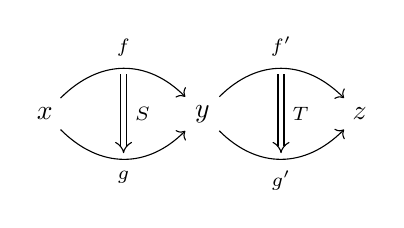
\begin{tikzpicture}
    \node (x) at (0,0) {$x$};
    \node (y) at (2,0) {$y$};
    \node (z) at (4,0) {$z$};
    \draw[->] (x) .. node[label={[label distance=-1mm]above:{\scriptsize$f$}}]{} controls (0.7,0.7) and (1.3,0.7) .. (y);
    \draw[->] (x) .. node[label={[label distance=-1mm]below:{\scriptsize$g$}}]{}controls (0.7,-0.7) and (1.3,-0.7) .. (y);
    \draw[double,double equal sign distance,-implies] (1,0.5) to node[label={[label distance=-1mm]right:{\scriptsize$S$}}]{} (1,-0.5);
    \draw[->] (y) .. node[label={[label distance=-1mm]above:{\scriptsize$f'$}}]{} controls (2.7,0.7) and (3.3,0.7) .. (z);
    \draw[->] (y) .. node[label={[label distance=-1mm]below:{\scriptsize$g'$}}]{}controls (2.7,-0.7) and (3.3,-0.7) .. (z);
    \draw[double,double equal sign distance,-implies] (3,0.5) to node[label={[label distance=-1mm]right:{\scriptsize$T$}}]{} (3,-0.5);
  \end{tikzpicture}
\] we get a \(2\)-morphism like this: \[
  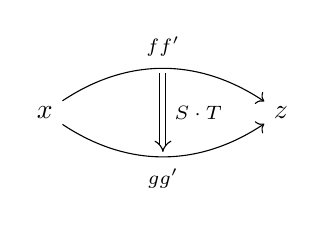
\begin{tikzpicture}[xscale=1.5]
    \node (x) at (0,0) {$x$};
    \node (z) at (2,0) {$z$};
    \draw[->] (x) .. node[label={[label distance=-1mm]above:{\scriptsize$ff'$}}]{} controls (0.7,0.7) and (1.3,0.7) .. (z);
    \draw[->] (x) .. node[label={[label distance=-1mm]below:{\scriptsize$gg'$}}]{}controls (0.7,-0.7) and (1.3,-0.7) .. (z);
    \draw[double,double equal sign distance,-implies] (1,0.5) to node[label={[label distance=-1mm]right:{\scriptsize$S\cdot T$}}]{} (1,-0.5);
  \end{tikzpicture}
\] But sometimes we can also horizontally compose a morphism and a
2-morphism! We can do it whenever our morphism \(f\) looks like a little
``whisker'' \(f\) sticking out of the \(2\)-morphism \(T\): \[
  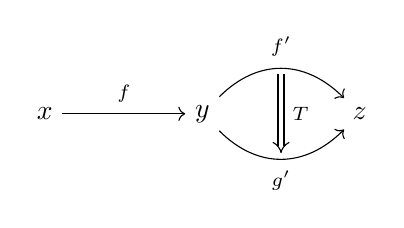
\begin{tikzpicture}
    \node (x) at (0,0) {$x$};
    \node (y) at (2,0) {$y$};
    \node (z) at (4,0) {$z$};
    \draw[->] (x) to node[label={[label distance=-1mm]above:{\scriptsize$f$}}]{} (y);
    \draw[->] (y) .. node[label={[label distance=-1mm]above:{\scriptsize$f'$}}]{} controls (2.7,0.7) and (3.3,0.7) .. (z);
    \draw[->] (y) .. node[label={[label distance=-1mm]below:{\scriptsize$g'$}}]{}controls (2.7,-0.7) and (3.3,-0.7) .. (z);
    \draw[double,double equal sign distance,-implies] (3,0.5) to node[label={[label distance=-1mm]right:{\scriptsize$T$}}]{} (3,-0.5);
  \end{tikzpicture}
\] and what we get is a \(2\)-morphism \(f\cdot S\) like this: \[
  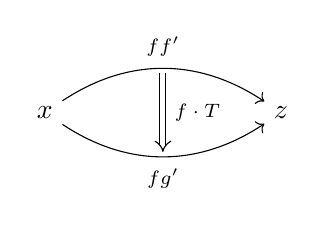
\begin{tikzpicture}[xscale=1.5]
    \node (x) at (0,0) {$x$};
    \node (z) at (2,0) {$z$};
    \draw[->] (x) .. node[label={[label distance=-1mm]above:{\scriptsize$ff'$}}]{} controls (0.7,0.7) and (1.3,0.7) .. (z);
    \draw[->] (x) .. node[label={[label distance=-1mm]below:{\scriptsize$fg'$}}]{}controls (0.7,-0.7) and (1.3,-0.7) .. (z);
    \draw[double,double equal sign distance,-implies] (1,0.5) to node[label={[label distance=-1mm]right:{\scriptsize$f\cdot T$}}]{} (1,-0.5);
  \end{tikzpicture}
\] This process, called ``whiskering'', is not really a new operation.
\(f\cdot S\) is really just the horizontal composite of these
\(2\)-morphisms: \[
  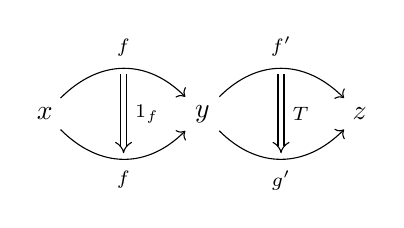
\begin{tikzpicture}
    \node (x) at (0,0) {$x$};
    \node (y) at (2,0) {$y$};
    \node (z) at (4,0) {$z$};
    \draw[->] (x) .. node[label={[label distance=-1mm]above:{\scriptsize$f$}}]{} controls (0.7,0.7) and (1.3,0.7) .. (y);
    \draw[->] (x) .. node[label={[label distance=-1mm]below:{\scriptsize$f$}}]{}controls (0.7,-0.7) and (1.3,-0.7) .. (y);
    \draw[double,double equal sign distance,-implies] (1,0.5) to node[label={[label distance=-1mm]right:{\scriptsize$1_f$}}]{} (1,-0.5);
    \draw[->] (y) .. node[label={[label distance=-1mm]above:{\scriptsize$f'$}}]{} controls (2.7,0.7) and (3.3,0.7) .. (z);
    \draw[->] (y) .. node[label={[label distance=-1mm]below:{\scriptsize$g'$}}]{}controls (2.7,-0.7) and (3.3,-0.7) .. (z);
    \draw[double,double equal sign distance,-implies] (3,0.5) to node[label={[label distance=-1mm]right:{\scriptsize$T$}}]{} (3,-0.5);
  \end{tikzpicture}
\] Similarly we can define \(T\cdot f\) in this sort of situation: \[
  \begin{tikzpicture}
    \node (x) at (0,0) {$x$};
    \node (y) at (2,0) {$y$};
    \node (z) at (4,0) {$z$};
    \draw[->] (x) .. node[label={[label distance=-1mm]above:{\scriptsize$f'$}}]{} controls (0.7,0.7) and (1.3,0.7) .. (y);
    \draw[->] (x) .. node[label={[label distance=-1mm]below:{\scriptsize$g'$}}]{}controls (0.7,-0.7) and (1.3,-0.7) .. (y);
    \draw[double,double equal sign distance,-implies] (1,0.5) to node[label={[label distance=-1mm]right:{\scriptsize$T$}}]{} (1,-0.5);
    \draw[->] (y) to node[label={[label distance=-1mm]above:{\scriptsize$f$}}]{} (z);
  \end{tikzpicture}
\] Anyway, once you're an expert on this \(2\)-categorical yoga, you can
easily see that these morphisms in \(\operatorname{Hom}(a,a)\), which
are really 2-morphisms in \(\mathsf{Ad}\): \[
  \begin{tikzcd}[column sep=huge]
    1_a
      \rar["i" description]
    & LR
      \rar[shift left=5,"i\cdot LR" description]
      \rar["LR\cdot i" description]
    & LRLR
      \rar[shift left=10,"i\cdot LRLR" description]
      \rar[shift left=5,"LR\cdot i\cdot LR" description]
      \rar["LRLR\cdot i" description]
      \lar[shift left=5,"L\cdot e\cdot R" description]
    & LRLRLR
      \lar[shift left=5,"L\cdot e\cdot RLR" description]
      \lar[shift left=10,"LRL\cdot e\cdot R" description]
      \rar
    &\ldots
  \end{tikzcd}
\] are obtained by taking our basic tiger stripe operations --- the
``merging of two black stripes'', or \(L\cdot e\cdot R\), and the
``appearance of a black stripe'', or \(i\) --- and drawing some extra
black stripes on both sides. That's what those \(LR\)'s are for. After
all, no tiger is complete without whiskers!

Okay. Now, having understood \(\operatorname{Hom}(a,a)\) in all these
ways, let's turn to \(\operatorname{Hom}(b,b)\). Luckily, this is very
similar! Here the objects are
\[1_b,\quad RL,\quad RLRL,\quad RLRLRL,\quad \ldots\] and morphisms are
pictures of \emph{orange} stripes on a \emph{black} background: \[
  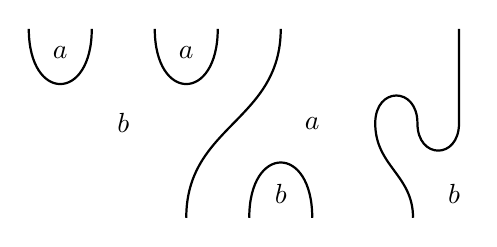
\begin{tikzpicture}[xscale=0.8,yscale=1.2]
    \begin{knot}
      \strand[thick] (-1,2)
        to [out=down,in=down,looseness=2] (0,2);
      \strand[thick] (1,2)
        to [out=down,in=down,looseness=2] (2,2);
      \strand[thick] (1.5,0)
        to [out=up,in=down](3,2);
      \strand[thick] (2.5,0)
        to [out=up,in=up,looseness=2] (3.5,0);
      \strand[thick] (5.1,0)
        to [out=up,in=down,looseness=1] (4.5,1)
        to [out=up,in=up,looseness=1.5] (5.17,1)
        to [out=down,in=down,looseness=1.5] (5.83,1)
        to (5.83,2);
    \end{knot}
    \node at (-0.5,1.75) {$a$};
    \node at (1.5,1.75) {$a$};
    \node at (0.5,1) {$b$};
    \node at (3.5,1) {$a$};
    \node at (3,0.25) {$b$};
    \node at (5.75,0.25) {$b$};
  \end{tikzpicture}
\] These orange stripes can only split: \[
  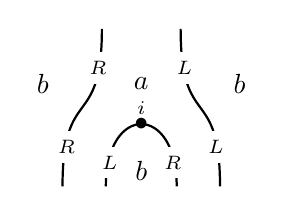
\begin{tikzpicture}[yscale=-2]
    \begin{knot}
      \strand[thick] (-0.5,0)
        to [out=up,in=down,looseness=1.5] (-1,1);
      \strand[thick] (-0.45,1)
        to [out=down,in=down,looseness=1.5] (0.45,1);
      \strand[thick] (0.5,0)
        to [out=up,in=down,looseness=1.5] (1,1);
    \end{knot}
    %
    \node at (-1.25,0.35) {$b$};
    \node at (0,0.35) {$a$};
    \node at (0,0.9) {$b$};
    \node at (1.25,0.35) {$b$};
    %
    \node[fill=white] at (-0.55,0.25) {\scriptsize$R$};
    \node[fill=white] at (-0.95,0.75) {\scriptsize$R$};
    \node[fill=white] at (-0.4,0.85) {\scriptsize$L$};
    \node[fill=white] at (0.4,0.85) {\scriptsize$R$};
    \node[fill=white] at (0.55,0.25) {\scriptsize$L$};
    \node[fill=white] at (0.95,0.75) {\scriptsize$L$};
    \node[label={[label distance=-2mm]above:{\scriptsize$i$}}] at (0,0.61) {$\bullet$};
  \end{tikzpicture}
\] or disappear: \[
  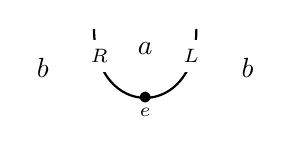
\begin{tikzpicture}[xscale=1.3,yscale=-1]
    \begin{knot}
      \strand[thick] (-0.5,0)
        to [out=up,in=up,looseness=3] (0.5,0);
    \end{knot}
    \node at (-1,0.5) {$b$};
    \node at (0,0.25) {$a$};
    \node at (1,0.5) {$b$};
    \node[fill=white] at (-0.45,0.35) {\scriptsize$R$};
    \node[fill=white] at (0.45,0.35) {\scriptsize$L$};
    \node[label={[label distance=-2mm]below:{\scriptsize$e$}}] at (0,0.88) {$\bullet$};
  \end{tikzpicture}
\] as we march down the page. This means is that
\(\operatorname{Hom}(b,b)\) is \(\Delta^{\mathrm{op}}\): the
\emph{opposite} of the category of simplices, the \emph{opposite} of the
category of finite ordinals, or the walking \emph{comonoid} --- which is
just like a monoid, only upside down!

Here is another picture of \(\operatorname{Hom}(b,b)\): \[
  \begin{tikzcd}[column sep=huge]
    1_b
    & RL
      \lar["e" description]
      \rar[shift left=5,"R\cdot i\cdot L" description]
    & RLRL
      \rar[shift left=10,"R\cdot i LRL" description]
      \rar[shift left=5,"RLR\cdot i\cdot L" description]
      \lar[shift left=5,"RL\cdot e" description]
      \lar["e\cdot RL" description]
    & RLRLRL
      \lar["e\cdot RLRL" description]
      \lar[shift left=5,"RL\cdot e\cdot RL" description]
      \lar[shift left=10,"RLRL\cdot e" description]
    &\ldots
      \lar
  \end{tikzcd}
\] If you're a devoted reader of This Week's Finds, you'll know I
secretly drew this category already in section N of
\protect\hyperlink{week118}{``Week 118''}. There I was talking about
specific adjoint functors instead of the walking adjunction, so as not
to prematurely blow your mind. I was also writing horizontal composites
backwards, for certain old-fashioned reasons. But the idea is exactly
the same! The morphisms above give the usual ``face and degeneracy
maps'' we always have in a simplicial set, since a simplicial set is a
functor \[F\colon \Delta^{\mathrm{op}} \to \mathsf{Set}.\] By the way,
you may have noticed that to get from \(\operatorname{Hom}(a,a)\) to
\(\operatorname{Hom}(b,b)\), we had to switch the colors orange and
black AND read the pictures upside-down. The reason is that if we turn
around all the \(1\)-morphisms AND \(2\)-morphisms in the walking
adjunction, we get the walking adjunction again. Ponder that!

We can summarize what we've learned so far using the ``Platonic idea''
jargon I introduced last week:

\begin{quote}
The Platonic idea of a monoid and the Platonic idea of a comonoid are
the hom-categories \(\operatorname{Hom}(a,a)\) and
\(\operatorname{Hom}(b,b)\) sitting inside the Platonic idea of an
adjunction!
\end{quote}

(By the way, to round this off we should really describe
\(\operatorname{Hom}(a,b)\) and \(\operatorname{Hom}(b,a)\), too. I
think \(\operatorname{Hom}(a,b)\) is the Platonic idea of ``an object
with a left action of a monoid and a right coaction of a comonoid, in a
compatible way''. If so, \(\operatorname{Hom}(b,a)\) would be the
Platonic idea of ``an object with a right action of a monoid and a left
coaction of a comonoid, in a compatible way''. By ``compatible'' I'm
saying that we can act on one side and coact on the other side in either
order, and get the same thing. Filling in the details requires concepts
I'm not eager to discuss right now, so I leave this as an exercise for
the highly energetic reader. The less energetic reader can just study
the tiger-stripe descriptions of these categories.)

Finally, here's Mueger's new twist on all these ideas! Better than an
adjunction is an ``ambidextrous'' adjunction. This has some extra
structure, which turns out to explain all sorts of fancy-sounding stuff
people look at in the study of subfactors and TQFTs and the like\ldots.

But what's an ``ambidextrous adjunction''?

A ambidextrous adjunction is where you have a morphism
\[L\colon a \to b\] in a \(2\)-category that is both left and right
adjoint to \[R\colon b \to a.\] More precisely, it is a setup
\[(a,b,L,R,i,e,j,f)\] where \[(a,b,L,R,i,e)\] and \[(b,a,R,L,j,f)\] are
both adjunctions.

In terms of string diagrams, our generating \(2\)-morphisms look like
this: \[
  \begin{gathered}
    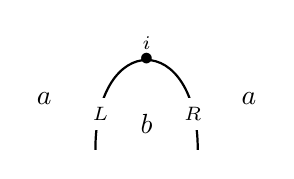
\begin{tikzpicture}[scale=1.3]
      \begin{knot}
        \strand[thick] (-0.5,0)
          to [out=up,in=up,looseness=3] (0.5,0);
      \end{knot}
      \node at (-1,0.5) {$a$};
      \node at (0,0.25) {$b$};
      \node at (1,0.5) {$a$};
      \node[fill=white] at (-0.45,0.35) {\scriptsize$L$};
      \node[fill=white] at (0.45,0.35) {\scriptsize$R$};
      \node[label={[label distance=-2mm]above:{\scriptsize$i$}}] at (0,0.88) {$\bullet$};
    \end{tikzpicture}
    \qquad
    \begin{tikzpicture}[scale=1.3]
      \begin{knot}
        \strand[thick] (-0.5,0)
          to [out=up,in=up,looseness=3] (0.5,0);
      \end{knot}
      \node at (-1,0.5) {$b$};
      \node at (0,0.25) {$a$};
      \node at (1,0.5) {$b$};
      \node[fill=white] at (-0.45,0.35) {\scriptsize$R$};
      \node[fill=white] at (0.45,0.35) {\scriptsize$L$};
      \node[label={[label distance=-2mm]above:{\scriptsize$j$}}] at (0,0.88) {$\bullet$};
    \end{tikzpicture}
  \\[2em]
    \begin{tikzpicture}[xscale=1.3,yscale=-1]
      \begin{knot}
        \strand[thick] (-0.5,0)
          to [out=up,in=up,looseness=3] (0.5,0);
      \end{knot}
      \node at (-1,0.5) {$b$};
      \node at (0,0.25) {$a$};
      \node at (1,0.5) {$b$};
      \node[fill=white] at (-0.45,0.35) {\scriptsize$R$};
      \node[fill=white] at (0.45,0.35) {\scriptsize$L$};
      \node[label={[label distance=-2mm]below:{\scriptsize$e$}}] at (0,0.88) {$\bullet$};
    \end{tikzpicture}
    \qquad
    \begin{tikzpicture}[xscale=1.3,yscale=-1]
      \begin{knot}
        \strand[thick] (-0.5,0)
          to [out=up,in=up,looseness=3] (0.5,0);
      \end{knot}
      \node at (-1,0.5) {$a$};
      \node at (0,0.25) {$b$};
      \node at (1,0.5) {$a$};
      \node[fill=white] at (-0.45,0.35) {\scriptsize$L$};
      \node[fill=white] at (0.45,0.35) {\scriptsize$R$};
      \node[label={[label distance=-2mm]below:{\scriptsize$f$}}] at (0,0.88) {$\bullet$};
    \end{tikzpicture}
  \end{gathered}
\] and the triangle equations say all possible zig-zags can be
straightened out.

Now let's study the ``walking ambidextrous adjunction'',
\(\mathsf{AmbAd}\). As before, \(2\)-morphisms in \(\mathsf{AmbAd}\) can
be described using pictures with orange and black stripes --- but now
\emph{both} kinds of stripes can appear, disappear, merge or split as we
march down the page: \[
  \begin{tikzpicture}[xscale=0.8,yscale=1.2]
    \begin{knot}
      \strand[thick] (-2,-2)
        to [out=up,in=down,looseness=0.7] (-1.5,0)
        to [out=up,in=down,looseness=0.7] (-2,2);
      \strand[thick] (-1,2)
        to [out=down,in=down,looseness=2] (0,2);
      \strand[thick] (1,2)
        to [out=down,in=down,looseness=2] (2,2);
      \strand[thick] (-1,-2)
        to [out=up,in=down] (-0.5,0.5)
        to [out=up,in=up,looseness=1.1] (0.5,0.5)
        to [out=down,in=up] (0.6,-2);
      \strand[thick] (0,0)
        to [out=right,in=right,looseness=0.8] (0,-1.5)
        to [out=left,in=right] (-0.25,-1.5)
        to [out=left,in=left,looseness=0.8] (0,0);
      \strand[thick] (1.5,-2)
        to (1.5,0)
        to [out=up,in=down](3,2);
      \strand[thick] (2.5,-2)
        to (2.5,0)
        to [out=up,in=up,looseness=1.1] (5,0)
        to [out=down,in=down,looseness=1.2] (6,0)
        to (6,2);
      \strand[thick] (3.3,-2)
        to (3.3,-1)
        to [out=up,in=up,looseness=1.5] (4.3,-1)
        to [out=down,in=up,looseness=1.3] (6,-2);
    \end{knot}
    %
    \node at (-1.95,0) {$a$};
    \node at (-0.5,1.75) {$a$};
    \node at (1.5,1.75) {$a$};
    \node at (-0.1,-0.8) {$b$};
    \node at (0,0.3) {$a$};
    \node at (0.5,1.2) {$b$};
    \node at (4.5,1.4) {$a$};
    \node at (3.8,0.1) {$b$};
    \node at (3.8,-1.25) {$a$};
    %
    \draw[thick] (-2.5,-2) rectangle ++(9.5,4);
  \end{tikzpicture}
\] This allows for quite arbitrary ways of cutting up a rectangle into
regions of orange and black, with piecewise linear boundaries, subject
to the condition that each vertical border has the same color all along
it. The triangle equations and the rules for \(2\)-categories say that
we can warp such a picture around without changing the \(2\)-morphism
that it defines\ldots{} I don't want to be too precise here, since it
would be boring. Hopefully you get the idea: \(\mathsf{AmbAd}\) has a
purely topological description!

Now for the punchline: in \(\mathsf{AmbAd}\), what is the category
\(\operatorname{Hom}(a,a)\) like? As in \(\mathsf{Ad}\), the objects are
\[1_a,\quad LR,\quad LRLR,\quad LRLRLR,\quad \ldots\] but now the object
\(LR\) is equipped not only with multiplication: \[
  \begin{tikzpicture}[yscale=2]
    \begin{knot}
      \strand[thick] (-0.5,0)
        to [out=up,in=down,looseness=1.5] (-1,1);
      \strand[thick] (-0.45,1)
        to [out=down,in=down,looseness=1.5] (0.45,1);
      \strand[thick] (0.5,0)
        to [out=up,in=down,looseness=1.5] (1,1);
    \end{knot}
    %
    \node at (-1.25,0.35) {$a$};
    \node at (0,0.35) {$b$};
    \node at (0,0.9) {$a$};
    \node at (1.25,0.35) {$a$};
    %
    \node[fill=white] at (-0.55,0.25) {\scriptsize$L$};
    \node[fill=white] at (-0.95,0.75) {\scriptsize$L$};
    \node[fill=white] at (-0.4,0.85) {\scriptsize$R$};
    \node[fill=white] at (0.4,0.85) {\scriptsize$L$};
    \node[fill=white] at (0.55,0.25) {\scriptsize$R$};
    \node[fill=white] at (0.95,0.75) {\scriptsize$R$};
    \node[label={[label distance=-2mm]below:{\scriptsize$e$}}] at (0,0.61) {$\bullet$};
    %
    \node at (0,-0.3) {multiplication:};
    \node at (0,-0.5) {$L\cdot e\cdot R\colon LRLR\Rightarrow LR$};
  \end{tikzpicture}
\] and multiplicative identity: \[
  \begin{tikzpicture}[scale=1.3]
    \begin{knot}
      \strand[thick] (-0.5,0)
        to [out=up,in=up,looseness=3] (0.5,0);
    \end{knot}
    \node at (-1,0.5) {$a$};
    \node at (0,0.25) {$b$};
    \node at (1,0.5) {$a$};
    \node[fill=white] at (-0.45,0.35) {\scriptsize$L$};
    \node[fill=white] at (0.45,0.35) {\scriptsize$R$};
    \node[label={[label distance=-2mm]above:{\scriptsize$i$}}] at (0,0.88) {$\bullet$};
    %
    \node at (0,-0.4) {multiplicative identity:};
    \node at (0,-0.75) {$i\colon 1_a\Rightarrow LR$};
  \end{tikzpicture}
\] but also a ``comultiplication'': \[
  \begin{tikzpicture}[yscale=2]
    \begin{scope}[yscale=-1,shift={(0,-1)}]
      \begin{knot}
        \strand[thick] (-0.5,0)
          to [out=up,in=down,looseness=1.5] (-1,1);
        \strand[thick] (-0.45,1)
          to [out=down,in=down,looseness=1.5] (0.45,1);
        \strand[thick] (0.5,0)
          to [out=up,in=down,looseness=1.5] (1,1);
      \end{knot}
      %
      \node at (-1.25,0.35) {$a$};
      \node at (0,0.35) {$b$};
      \node at (0,0.9) {$a$};
      \node at (1.25,0.35) {$a$};
      %
      \node[fill=white] at (-0.55,0.25) {\scriptsize$L$};
      \node[fill=white] at (-0.95,0.75) {\scriptsize$L$};
      \node[fill=white] at (-0.4,0.85) {\scriptsize$R$};
      \node[fill=white] at (0.4,0.85) {\scriptsize$L$};
      \node[fill=white] at (0.55,0.25) {\scriptsize$R$};
      \node[fill=white] at (0.95,0.75) {\scriptsize$R$};
      \node[label={[label distance=-2mm]above:{\scriptsize$j$}}] at (0,0.61) {$\bullet$};
    \end{scope}
    %
    \node at (0,-0.3) {comultiplication:};
    \node at (0,-0.5) {$L\cdot j\cdot R\colon LR\Rightarrow LRLR$};
  \end{tikzpicture}
\] and ``comultiplicative coidentity'': \[
  \begin{tikzpicture}[scale=1.3]
    \begin{scope}[yscale=-1,shift={(0,-1)}]
      \begin{knot}
        \strand[thick] (-0.5,0)
          to [out=up,in=up,looseness=3] (0.5,0);
      \end{knot}
      \node at (-1,0.5) {$a$};
      \node at (0,0.25) {$b$};
      \node at (1,0.5) {$a$};
      \node[fill=white] at (-0.45,0.35) {\scriptsize$L$};
      \node[fill=white] at (0.45,0.35) {\scriptsize$R$};
      \node[label={[label distance=-2mm]below:{\scriptsize$f$}}] at (0,0.88) {$\bullet$};
    \end{scope}
    %
    \node at (0,-0.5) {comultiplicative identity:};
    \node at (0,-0.85) {$f\colon LR\Rightarrow 1_a$};
  \end{tikzpicture}
\] which make it into a monoid object \emph{and} a comonoid object. Even
better, there are some extra relations between the multiplication and
comultiplication, which make \(LR\) into a so-called ``Frobenius
object''!

In short, \(\operatorname{Hom}(a,a)\) is the walking Frobenius object!
So is \(\operatorname{Hom}(b,b)\), since there is no real asymmetry
between the objects \(a\) and \(b\) in an ambidextrous adjunction, as
there was with an adjunction. I haven't thought much about
\(\operatorname{Hom}(a,b)\) and \(\operatorname{Hom}(b,a)\) yet, but one
obvious thing is that they're isomorphic.

Next time I'll talk about examples of Frobenius objects and why they are
so important in subfactors, TQFTs and the like. This is what Mueger is
really interested in. Right now, I want to wrap up by saying exactly
what it means to say \(LR\) is a ``Frobenius object''. What are the
extra relations between multiplication and comultiplication?

There are various ways of describing these relations. Mueger uses a pair
of equations that are popular in the TQFT literature: \[
  \begin{tikzpicture}[yscale=2]
    \begin{knot}
      \strand[thick] (-1,-1.5)
        to [out=up,in=down,looseness=1.5] (-0.4,-0.5)
        to (-0.4,0)
        to [out=up,in=down,looseness=1.5] (-1,1);
      \strand[thick] (-0.45,1)
        to [out=down,in=down,looseness=1.5] (0.45,1);
      \strand[thick] (-0.45,-1.5)
        to [out=up,in=up,looseness=1.5] (0.45,-1.5);
      \strand[thick] (1,-1.5)
        to [out=up,in=down,looseness=1.5] (0.4,-0.5)
        to (0.4,0)
        to [out=up,in=down,looseness=1.5] (1,1);
    \end{knot}
    %
    \node at (-1.25,-0.25) {$a$};
    \node at (0,-0.25) {$b$};
    \node at (0,0.9) {$a$};
    \node at (1.25,-0.25) {$a$};
    \node at (0,-1.4) {$a$};
  \end{tikzpicture}
  \qquad
  \raisebox{7em}{$=$}
  \qquad
  \begin{tikzpicture}[yscale=2]
    \begin{knot}
      \strand[thick] (-1,-1.5) to (-1,1);
      \strand[thick] (-0.5,-1.5)
        to (-0.5,-0.5)
        to [out=up,in=left] (-0.25,-0.35)
        to [out=right,in=up,looseness=0.6] (0.5,-1.25)
        to (0.5,-1.5);
      \strand[thick] (0.5,1)
        to (0.5,0)
        to [out=down,in=right] (0.25,-0.15)
        to [out=left,in=down,looseness=0.6] (-0.5,0.75)
        to (-0.5,1);
      \strand[thick] (1,-1.5) to (1,1);
    \end{knot}
    \node at (-1.5,-0.25) {$a$};
    \node at (0,0.75) {$a$};
    \node at (0,-0.25) {$b$};
    \node at (0,-1) {$a$};
    \node at (1.5,-0.25) {$a$};
  \end{tikzpicture}
\] and its mirror image. People sometimes call these the ``\(I = N\)''
equations, for the obvious reason. So: one definition of a ``Frobenius
object'' in a monoidal category is that it's a monoid object / comonoid
object satisfying the \(I = N\) equations.

Where can you read about this? Well, besides Mueger's paper, there are
these:

\begin{enumerate}
\def\labelenumi{\arabic{enumi})}
\setcounter{enumi}{3}
\item
  Frank Quinn, ``Lectures on axiomatic quantum field theory'', in
  \emph{Geometry and Quantum Field Theory}, Amer. Math. Soc.,
  Providence, RI, 1995.
\item
  Lowell Abrams, ``Two-dimensional topological quantum field theories
  and Frobenius algebras'', \emph{J. Knot Theory and its Ramifications}
  \textbf{5} (1996), 569--587.
\end{enumerate}

A ``Frobenius algebra'' is just a Frobenius object in the category of
vector spaces. I seem to recall that this is equivalent to what Quinn
calls an ``ambialgebra''. For any TQFT in any dimension, the vector
space associated to the sphere is a commutative Frobenius algebra. The
proof consists of playing with pictures very much like the ones above,
but in higher dimensions.

The \(I = N\) equations are cute, but personally I prefer a more
conceptual description of a Frobenius object. This may be a bit
mindblowing to the uninitiated, so if you're just barely hanging on,
please stop now.

Hmm! If you're still reading this, you must be brave! Okay --- don't say
I didn't warn you. Let's start by pondering \(LR\) a bit more. This guy
is its own adjoint, with the unit and counit as follows: \[
  \begin{tikzpicture}[yscale=2]
    \begin{scope}[yscale=-1,shift={(0,-0.75)}]
      \begin{knot}
        \strand[thick] (-0.5,0)
          to [out=up,in=down,looseness=1.5] (-1,1);
        \strand[thick] (-0.45,1)
          to [out=down,in=down,looseness=1.5] (0.45,1);
        \strand[thick] (0.5,0)
          to [out=up,in=down,looseness=1.5] (1,1);
        \strand[thick] (-0.5,0)
          to [out=down,in=down] (0.5,0);
      \end{knot}
      %
      \node at (-1.25,0.35) {$a$};
      \node at (0,0.35) {$b$};
      \node at (0,0.9) {$a$};
      \node at (1.25,0.35) {$a$};
    \end{scope}
    %
    \node at (0,-0.5) {unit for $LR$:};
    \node at (0,-0.75) {multiplicative identity};
    \node at (0,-0.95) {composed with comultiplication};
  \end{tikzpicture}
  \qquad
  \begin{tikzpicture}[yscale=2]
    \begin{knot}
      \strand[thick] (-0.5,0)
        to [out=up,in=down,looseness=1.5] (-1,1);
      \strand[thick] (-0.45,1)
        to [out=down,in=down,looseness=1.5] (0.45,1);
      \strand[thick] (0.5,0)
        to [out=up,in=down,looseness=1.5] (1,1);
      \strand[thick] (-0.5,0)
        to [out=down,in=down] (0.5,0);
    \end{knot}
    %
    \node at (-1.25,0.35) {$a$};
    \node at (0,0.35) {$b$};
    \node at (0,0.9) {$a$};
    \node at (1.25,0.35) {$a$};
    %
    \node at (0,-0.5) {counit for $LR$:};
    \node at (0,-0.75) {multiplication composed with};
    \node at (0,-0.95) {comultiplicative coidentity};
  \end{tikzpicture}
\] It's easy to check the triangle equations by straightening out the
relevant zig-zags.

Now, whenever a monoid object has a right or left adjoint, that right or
left adjoint automatically becomes a comonoid object, by the magic of
duality. But if a monoid object is its \emph{own} adjoint, it becomes a
comonoid object in \emph{two} ways, because it is both its own left
\emph{and} right adjoint! So, our guy \(LR\) is a comonoid object in
\emph{three} ways! Huh? Well, we already knew \(LR\) was a comonoid
object before this devilish paragraph began, but since \(LR\) is its own
adjoint, it becomes a comonoid object in two other ways. Amazingly, the
\(I = N\) equations are equivalent to the fact that all three comonoid
structures agree! I leave this as an exercise for the insanely energetic
reader\ldots{} I've worked it out before, and I rechecked it this
morning in bed. I don't know if a proof exists in the literature, but
from what Mueger writes, I suspect maybe you can catch glimpses of it in
Appendix A3 of this book:

\begin{enumerate}
\def\labelenumi{\arabic{enumi})}
\setcounter{enumi}{5}
\tightlist
\item
  L. Kadison, \emph{New Examples of Frobenius Extensions}, University
  Lecture Series \#\textbf{14}, Amer. Math. Soc., Providence RI, 1999.
\end{enumerate}

Anyway, the upshot is that we can equivalently define a Frobenius object
in a monoidal category as follows: it's a monoid object / comonoid
object which becomes its own adjoint by letting

\begin{itemize}
\tightlist
\item
  unit = multiplicative identity composed with comultiplication
\item
  counit = multiplication composed with comultiplicative coidentity
\end{itemize}

and has the property that the resulting 3 comonoid structures agree.

Or, equivalently, that the resulting 3 monoid structures agree!

There is much more to say about this, but let's stop here.

\begin{center}\rule{0.5\linewidth}{0.5pt}\end{center}

Postscript --- Oswald Wyler had this correction to make:

\begin{quote}
The walking adjunction is much older than the 1986 paper by Schanuel and
Street. Back in 1970, Pumplün published a paper: ``Eine Bemerkung über
Monaden und adjungierte Funktoren'', \emph{Math. Annalen} \textbf{185}
(1970), 329--377. The small bicategory ``walking adjunction'' definitely
was in that paper, but I don't recall whether it was explicitly
formulated or not.
\end{quote}

Andree Ehresmann added:

\begin{quote}
On the ``walking adjunction''

I don't know the Pumplun's paper cited by Wyler. But there is another
reference at about the same time; indeed, the ``walking adjunction'' has
been explicitly constructed and studied in the paper of Auderset:

``Adjonction et monade au niveau des \(2\)-categories''

published in \emph{Cahiers de Top. et Geom. Diff.} \textbf{XV-1} (1974),
3--20.

More formally it could also be called ``the 2-sketch of an adjunction''
in the terminology in my paper with Charles Ehresmann:

``Categories of sketched structures'', in the \emph{Cahiers}
\textbf{XIII-2} (1972),

reprinted in ``Charles Ehresmann: Oeuvres completes et commentees'' Part
\textbf{IV-2}.
\end{quote}

Bill Lawvere added:

\begin{quote}
\textbf{ONE MORE HISTORICAL CITATION}

The Pumplun paper cited by Wyler as well as the Auderset paper cited by
Mme Ehresmann illustrate that the study of generic structures in
\(2\)-categories has been going on for some time. My own paper ORDINAL
SUMS AND EQUATIONAL DOCTRINES, SLNM 80 (1969) 141--155 shows that the
augmented simplicial category \(\Delta\) serves as the generic monad,
but moreover goes on to actually apply this to show that the Kleisli
construction is a tensor product left-adjoint to the Eilenberg- Moore
construction which is an enriched Hom. The Hom/tensor formalism
appropriate to the case of strict monoid objects is all that is required
here, as I will explain below.

\textbf{AN EXTENSION AND A RESTRICTION}

The important special case of FROBENIUS monads is explicitly
characterized in three ways in my paper. Concerning the IDEMPOTENT case
discussed a few days ago by Grandis and Johnstone, note that the
publication of Schanuel and Street proves among other things that the
monoid \(\Delta\) in \(\mathsf{Cat}\) has very few quotients (see below
for significance of the monoid structure).

\textbf{THE GENERAL HOM/TENSOR FORMALISM AND A VERY PARTICULAR MONOID}

In any cartesian-closed category with finite limits and co-limits, a
non-linear version of the Cartan-Eilenberg Hom/tensor formalism applies
to actions and biactions of monoid objects. In Cat, \(\Delta\) is a
(strict) monoid and its actions are precisely monads on arbitrary
categories. A crucial part of the formalism is that categories of
actions are automatically enriched in the basic cartesian-closed
category, which in this case is Cat. There is a particular biaction of
\(\Delta\), which I called \(\Delta\) plus, with the property that the
enriched Hom of it into an arbitrary \(\Delta\)-action is exactly the
Eilenberg-Moore category of ``algebras'', automatically equipped with
its structure as a \(\Delta^{\mathrm{op}}\) action (co-monad). The
left-adjoint tensor assigns to any category equipped with a co-monad its
Kleisli category, as a category with monad. Not only are the
calculations in this particular case quite explicit, but the enriched
Hom tensor formalism has a lot of content which is still
under-exploited.

\textbf{SKETCHES VERSUS PLATONISM}

The often repeated slander that mathematicians think ``as if'' they were
``platonists'' needs to be combatted rather than swallowed. What
mathematicians and other scientists use is the objectively developed
human instrument of general concepts. (The plan to misleadingly use that
fact as a support for philosophical idealism may have been an honest
mistake by Plato, or it may have been part of his job as disinformation
officer for the Athenian CIA organization; it probably would not have
survived until now had it not been for the special efforts of Cosimo de'
Medici.) It seems that a general concept has two related aspects, as I
began to realize more explicitly in connection with my paper
``Adjointness in foundations'', \emph{Dialectica} vol. \textbf{23}
(1969), pp.~281--296; I later learned that some philosophers refer to
these two aspects as ``abstract general vs.~concrete general''. For
example, there is the algebraic theory of rings vs.~the category of all
rings, or a particular abstract group vs.~the category of all
permutation representations of the group. While it is ``obvious'' that,
at least in mathematics, a concrete general should have the structure of
a category, because all the instances embody the same abstract general
and hence any two instances can be compared in preferred ways, by
contrast it was not until the late fifties that one realized that an
abstract general can also be construed as a category in its own right.
That realization essentially made explicit the fact that substitution is
a logical operation and indeed is the most fundamental logical
operation.

Thus an abstract general is essentially a special algebraic structure
indeed a category with additional structure such as finite limits or
still richer doctrines. As with other algebraic structures there are
again two aspects, the structures themselves and their presentations
which are closely related, yet quite distinct; for example, more than
one presentation may be needed for efficient calculations determining
features of the same algebraic structure. What is meant by a
presentation depends on the doctrine: for example \(\Delta\) as a mere
category has an infinite presentation used in topology, but as a strict
monoidal category it has a finite presentation.

The notion of SKETCH is the most efficient scheme yet devised for the
general construction of PRESENTATIONS OF ABSTRACT GENERALS. The fact
that particular abstract generals and the idea of sketches exist within
the historically developed objective science does not mean that they
somehow always existed; to call them ``platonic'' seems to detract from
the honor of their actual discoverers.

Bill Lawvere
\end{quote}



\hypertarget{week175}{%
\section{December 29, 2001}\label{week175}}

I spent this Christmas in Greenwich, England. Over repeated visits to
England I have discovered many fascinating things of which many
Americans are unaware. For example: while in traffic one must drive on
the left side of the road, in escalators one must stand on the right.
You flip switches down to turn on lights. Camels and zebras have escaped
from the Royal Zoo and mated, and their hybrids roam the English
countryside. On the roadside you will occasionally see signs for
``humped zebra crossings''. Also, the Royal Observatory in Greenwich
fires a powerful green laser each night to mark the Prime Meridian ---
zero degrees longitude.

Four of the last five sentences are true. In particular, you really
\emph{can} see a green laser beam shining due north from the Royal
Observatory, across the Thames, past the Citigroup Building and out into
the night. And speaking of longitude, the day before Christmas I visited
this observatory and had a wonderful time learning how John Harrison
solved the longitude problem.

The longitude problem? Ah, how soon we forget! It's pretty easy to tell
your latitude by looking at the sun or the stars. However, it's pretty
hard to tell your longitude, unless you have a clock that keeps good
time. After all, if you know what time it is in a fixed place, like
Greenwich, you can figure out how far east or west you've gone by
comparing the time you see the sun rise to the time it would rise there.
Unfortunately, until the late 1700's, pendulum clocks didn't work well
at sea, due to the rocking waves. This was a real problem! Ships would
lose track of their longitude, go astray, and sometimes even run
aground, killing hundreds of sailors.

Since England was a big maritime power, in 1714 they set up the Board of
Longitude, which offered a prize of 20,000 pounds to anyone who could
solve this problem. Newton and Halley favored a solution which involved
measuring the angle between the moon and nearby stars and then
consulting a bunch of tables. This was a complicated system that could
only work with the help of an accurate star atlas and a detailed
understanding of the motion of the moon. Newton set to work on the
necessary calculations. John Flamsteed was made the royal astronomer of
England, and he set to work on the star atlas. He moved into the Royal
Observatory, and stayed up each night making observations with the help
of his wife.

However, before this ``lunar distance method'' came online, the
watchmaker John Harrison invented the first of a series of ingenious
clocks that worked well despite rocking waves and fluctuations of
temperature. All these can still be seen at the Royal Observatory ---
they're very beautiful! In the process, Harrison developed a whole bunch
of cool technology like ball bearings and the bimetallic strip used in
thermostats.

Alas, the Board refused to pay up even when Harrison built a clock that
was accurate to within .06 seconds a day, which was certainly good
enough. Finally King George III persuaded the board to give him the
prize --- but by then he was an old man. Luckily, I get the feeling
Harrison was really more interested in building clocks than winning the
prize money. He loved his work\ldots{} one of the keys to a happy life.

Here's a book that tells his story in more detail:

\begin{enumerate}
\def\labelenumi{\arabic{enumi})}
\tightlist
\item
  Dava Sobel, \emph{Longitude}, Fourth Estate Ltd., London, 1996.
\end{enumerate}

I found it in the gift shop of the Observatory. It's a fun read, but for
the technical reader it's frustratingly vague on the technical details
of how Harrisons' clocks actually work.

I also bought this book there:

\begin{enumerate}
\def\labelenumi{\arabic{enumi})}
\setcounter{enumi}{1}
\tightlist
\item
  E. G. Richards, \emph{Mapping Time: The Calendar and its History},
  Oxford U. Press, Oxford, 1998.
\end{enumerate}

Since it's almost New Year's Day, let me tell you a bit what I learned
about calendars!

Mathematical physics has deep roots in astronomy, which may have been
the first exact science. Thanks to astrology, the ancient theocratic
states put a lot of resources into precisely tracking and predicting the
motion of the sun, moon and planets. For example, by 700 BC the
Babylonians had measured the length of the year to be 365.24579 days,
with an error of only .00344 days. Two hundred years later, they had
measured the length of the month to be 29.53014 days --- an error of
only 2.6 seconds.

If there were 360 days in a year, 30 days in a month, and 12 months in a
year, the ancients would have been happy, since they loved numbers with
lots of divisors. But alas, there aren't! These whole numbers come
tantalizingly close, but not close enough, so the need for accurate
calendars, balanced by the desire for simplicity, kept pushing the
development of mathematics and astronomy forward.

There are also lots of complications I haven't mentioned. I've been
talking about the ``mean solar day'', the ``mean synodic month'' and the
``tropical year'', but in fact the length of the day and month vary
substantially due to the tilt of the earth's axis, the tilt of the
moon's orbit, and other effects --- so actually there are several
different definitions of day, month and year. This was enough to keep
the astronomer-priests in business for centuries. For more on the
physics of it all, try:

\begin{enumerate}
\def\labelenumi{\arabic{enumi})}
\setcounter{enumi}{2}
\tightlist
\item
  John Baez, ``The wobbling of the earth and other curiosities'',
  \texttt{http://math.ucr.edu/home/baez/wobble.html}
\end{enumerate}

Unfortunately, the Romans, whose calendar we inherit, were real
goofballs when it came to calendrics. Their system was run by a body of
``pontifices'' headed by the Pontifex Maximus. In 450 BC these guys
adopted a calendar in which odd-numbered years had 12 months and 355
days, while even-numbered years had 13 months and alternated between 377
and 378 days. The extra month, called Mercedonius, was stuck smack in
the middle of February. Even worse, this system gave an average of 366
and \(1/4\) days per year --- one too many --- so it kept drifting out
of kilter with the seasons. The pontifices were authorized to fix things
on an ad hoc basis as needed, but power corrupts, so they started taking
bribes to suddenly advance or postpone the start of the year.

As a result, by the time Julius Caesar became dictator, the calendar was
three months in advance of the seasons! After consulting with the
Alexandrian astronomer Sosigenes, he decided to institute reforms. To
straighten things out, the year 46 BC was made 445 days long. This was
known as the Last Year of Confusion. It featured an extra long
Mercedonius as well as two extra months after December, called
Undecimber and Duodecimber.

The new so-called ``Julian calendar'' featured 12 months and 365 days,
with an extra day in February every fourth year. The months alternated
nicely between 31 and 30 days, except for February, which only had 30 on
leap years. Unfortunately, Caesar was assassinated in 44 BC before this
system fully took hold. The pontifices ineptly interpreted his orders
and stuck in an extra day every \emph{third} year. This didn't get fixed
until 9 BC, Augustus stopped this practice and decreed that the next 3
leap years be skipped to make up for the extra ones the pontifices had
inserted.

From then on, things went more smoothly, except for a lot of
name-grabbing. When Julius Caesar was assassinated, the Senate took the
month of Quintilis and renamed it ``Iulius'' in his honor, giving us
July. Augustus followed suit, naming the month of Sextilis after himself
--- giving us August. More annoyingly, he stole the last day from
February and stuck it on his own month to make it 31 days long, and did
some extra reshuffling so the months next to his had only 30 --- giving
us our current messy setup.

The Senate offered to name a month after the next emperor, Tiberius, but
he modestly declined. The next one, Caligula, was not so modest: he
renamed June after his father Germanicus. Then Claudius renamed May
after himself, and Nero grabbed April. Later, Domitian took October and
Antonius took September. The vile Commodus tried to rename all twelve
months, but that didn't stick. Then Tacitus snatched September away from
Antonius\ldots{} but luckily, all these later developments have been
forgotten!

This is only a tiny fraction of the fascinating lore in Richards' book.
Ever wonder why there are 7 days in a week? That's pretty easy: they're
named after the 7 planets --- in the old sense of ``planets'', meaning
heavenly bodies visible by eye that don't move with the stars. But
here's a harder puzzle! Why are the 7 planets are listed in this order?

\begin{longtable}[]{@{}ll@{}}
\toprule
\endhead
Sun & (Sunday --- \emph{Dies Solis})\tabularnewline
Moon & (Monday --- \emph{Dies Lunae})\tabularnewline
Mars & (Tuesday --- \emph{Dies Martis})\tabularnewline
Mercury & (Wednesday --- \emph{Dies Mercurii})\tabularnewline
Jupiter & (Thursday --- \emph{Dies Iovis})\tabularnewline
Venus & (Friday --- \emph{Dies Veneris})\tabularnewline
Saturn & (Saturday --- \emph{Dies Saturnis})\tabularnewline
\bottomrule
\end{longtable}

There's actually a nice explanation. However, I won't give it away here.
Can you guess it?

Since ancient science was closely tied to numerology, I can't resist
mentioning some fun facts relating the calendar and the deck of cards.
As you probably know, playing cards come in 4 suits of 13 cards each,
for a total of 52. 52 is also the number of weeks in a year. The 4
suites correspond to the 4 seasons, so there are 13 weeks in each
season, just as there are 13 cards in each suite.

Even better, if we add up the face values of all the cards in the deck,
counting an ace as 1, a deuce as 2, and so on up to 13, we get
\[(1 + 2 + 3 + 4 + 5 + 6 + 7 + 8 + 9 + 10 + 11 + 12 + 13) \times 4 = 364,\]
which is one less than the number of days in a year! The remaining day
corresponds to the ``joker'', a card which does not belong to any suite.

Many calendars contain ``epagomenal days'' not included in any month.
For example, the Egyptians had 5 epagomenal days, leaving 360 which they
could split up neatly into 12 months. In a system with one epagomenal
day --- the ``joker'' --- the remaining 364 days can be divided not only
as \[(30 + 30 + 31) \times 4,\] which allows for two 30-day calendar
months and one 31-day calendar month per season, but also as
\[13 \times 28\] which allows for 13 anomalistic months of 28 days each
--- where an ``anomalistic month'' is the time it takes for the moon to
come round to its perigee, where it's as close to the earth as possible.

Putting it all together, we see that the number 364 factors as
\[13 \times 4 \times 7,\] which corresponds to 13 months, each
containing 4 weeks, each containing 7 days --- or alternatively to 4
seasons, each containing 13 weeks, each containing 7 days --- or to 4
suites, each containing 13 cards, with an average face value of 7.

Cute, eh? I'm not sure how much of this stuff is coincidence and how
much was planned out by the mysterious mystics who invented playing
cards. Of course we can't take these whole numbers too seriously --- for
example, the anomalistic month is actually 27.55455 days long, not 28.
However, a 364-day year \emph{is} mentioned in the the Book of Enoch, a
pseudepigrapical Hebrew text which was found, among other places, in the
Dead Sea Scrolls. In fact, a year of this length was used in Iceland as
late as 1940. The idea of having one epagomenal day and dividing each
season into months with 30, 30 and 31 days has also been favored by many
advocates of calendar reform.

Of course, numerology should always be left to competent mathematicians
who don't actually believe in it.

Here's another nice book:

\begin{enumerate}
\def\labelenumi{\arabic{enumi})}
\setcounter{enumi}{3}
\tightlist
\item
  Alain Connes, Andre Lichnerowicz and Marcel Paul Schutzenberger,
  \emph{A Triangle of Thoughts}, AMS, Providence, 2000.
\end{enumerate}

This consists of polished-up transcripts of dialogues (or should I say
trialogues?) among these mathematicians. I wish more good scientists
would write this sort of thing; it's much less strenuous to learn stuff
by listening to people talk than by reading textbooks! It's true that
textbooks are necessary when you want to master the details, but for the
all-important ``big picture'', conversations can be much better.

This book focuses on mathematical logic and physics, with a strong touch
of philosophy\ldots{} but it wanders all over the map in a pleasant way
--- from Bernoulli numbers to game theory! The conversation is dominated
by Connes, whose name appears on the title in bigger letters than the
other two authors, perhaps because they others are now dead.

There is only one mistake in this book that I would like to complain
about. Following Roger Penrose, Connes takes quasicrystals as evidence
for some mysterious uncomputability in the laws of nature. The idea is
that since there's no algorithm for deciding when a patch of Penrose
tiles can be extended to a tiling of the whole plane, nature must do
something uncomputable to produce quasicrystals of this symmetry. The
flaw in this reasoning seems obvious: when nature gets stuck, it feels
free to insert a \emph{defect} in the quasicrystal. Quasicrystals do not
need to be perfect to produce the characteristic diffraction patterns by
which we recognize them.

But that's a minor nitpick: the book is wonderful! Read it!

In case you don't know: Alain Connes is a Fields medalist, who won the
prize mainly for two things: his work on Von Neumann algebras, and his
work on noncommutative geometry. Now I'll talk a bit about von Neumann
algebras, since you'll need to understand a bit about them to follow the
rest of my description of the paper by Michael Mueger that I have been
slowly explaining throughout \protect\hyperlink{week173}{``Week 173''}
and \protect\hyperlink{week174}{``Week 174''}.

So: what's a von Neumann algebra? Before I get technical and you all
leave, I should just say that von Neumann designed these algebras to be
good ``algebras of observables'' in quantum theory. The simplest example
consists of all \(n\times n\) complex matrices: these become an algebra
if you add and multiply them the usual way. So, the subject of von
Neumann algebras is really just a grand generalization of the theory of
matrix multiplication.

But enough beating around the bush! For starters, a von Neumann algebra
is a \(*\)-algebra of bounded operators on some Hilbert space of
countable dimension --- that is, a bunch of bounded operators closed
under addition, multiplication, scalar multiplication, and taking
adjoints: that's the \(*\) business. However, to be a von Neumann
algebra, our \(*\)-algebra needs one extra property! This extra property
is cleverly chosen so that we can apply functions to observables and get
new observables, which is something we do all the time in physics.

More precisely, given any self-adjoint operator \(A\) in our von Neumann
algebra and any measurable function \(f\colon\mathbb{R}\to\mathbb{R}\),
we want there to be a self-adjoint operator \(f(A)\) that again lies in
our von Neumann algebra. To make sure this works, we need our von
Neumann algebra to be ``closed'' in a certain sense. The nice thing is
that we can state this closure property either algebraically or
topologically.

In the algebraic approach, we define the ``commutant'' of a bunch of
operators to be the set of operators that commute with all of them. We
then say a von Neumann algebra is a \(*\)-algebra of operators that's
the commutant of its commutant.

In the topological approach, we say a bunch of operators \(T_i\)
converges ``weakly'' to an operator \(T\) if their expectation values
converge to that of \(T\) in every state, that is,
\[\langle\psi, T_i\psi \rangle \to \langle\psi, T\psi\rangle\] for all
unit vectors \(\psi\) in the Hilbert space. We then say a von Neumann
algebra is an \(*\)-algebra of operators that is closed in the weak
topology.

It's a nontrivial theorem that these two definitions agree!

While classifying all \(*\)-algebras of operators is an utterly hopeless
task, classifying von Neumann algebras is almost within reach --- close
enough to be tantalizing, anyway. Every von Neumann algebra can be built
from so-called ``simple'' ones as a direct sum, or more generally a
``direct integral'', which is a kind of continuous version of a direct
sum. As usual in algebra, the ``simple'' von Neumann algebras are
defined to be those without any nontrivial ideals. This turns out to be
equivalent to saying that only scalar multiples of the identity commute
with everything in the von Neumann algebra.

People call simple von Neumann algebras ``factors'' for short. Anyway,
the point is that we just need to classify the factors: the process of
sticking these together to get the other von Neumann algebras is not
tricky.

The first step in classifying factors was done by von Neumann and
Murray, who divided them into types \(\mathrm{I}\), \(\mathrm{II}\), and
\(\mathrm{III}\). This classification involves the concept of a
``trace'', which is a generalization of the usual trace of a matrix.

Here's the definition of a trace on a von Neumann algebra. First, we say
an element of a von Neumann algebra is ``nonnegative'' if it's of the
form \(xx^*\) for some element \(x\). The nonnegative elements form a
``cone'': they are closed under addition and under multiplication by
nonnegative scalars. Let \(P\) be the cone of nonnegative elements. Then
a ``trace'' is a function \[\operatorname{tr}\colon P \to [0, +\infty]\]
which is linear in the obvious sense and satisfies
\[\operatorname{tr}(xy) = \operatorname{tr}(yx)\] whenever both \(xy\)
and \(yx\) are nonnegative.

Note: we allow the trace to be infinite, since the interesting von
Neumann algebras are infinite-dimensional. This is why we define the
trace only on nonnegative elements; otherwise we get
``\(\infty minus \infty\)'' problems. The same thing shows up in the
measure theory, where we start by integrating nonnegative functions,
possibly getting the answer \(+\infty\), and worry later about other
functions.

Indeed, a trace very much like an integral, so we're really studying a
noncommutative version of the theory of integration. On the other hand,
in the matrix case, the trace of a projection operator is just the
dimension of the space it's the projection onto. We can define a
``projection'' in any von Neumann algebra to be an operator with
\(p^* = p\) and \(p^2 = p\). If we study the trace of such a thing,
we're studying a \emph{generalization of the concept of dimension}. It
turns out this can be infinite, or even nonintegral!

We say a factor is type \(\mathrm{I}\) if it admits a nonzero trace for
which the trace of a projection lies in the set
\(\{0,1,2,\ldots,+\infty\}\). We say it's type \(I_n\) if we can
normalize the trace so we get the values \(\{0,1,\ldots,n\}\).
Otherwise, we say it's type \(I_\infty\), and we can normalize the trace
to get all the values \(\{0,1,2,\ldots,+\infty\}\).

It turn out that every type \(I_n\) factor is isomorphic to the algebra
of \(n\times n\) matrices. Also, every type \(I_\infty\) factor is
isomorphic to the algebra of all bounded operators on a Hilbert space of
countably infinite dimension.

Type \(\mathrm{I}\) factors are the algebras of observables that we
learn to love in quantum mechanics. So, the real achievement of von
Neumann was to begin exploring the other factors, which turned out to be
important in quantum field theory.

We say a factor is type \(\mathrm{II}_1\) if it admits a trace whose
values on projections are all the numbers in the unit interval
\([0,1]\). We say it is type \(\mathrm{II}_\infty\) if it admits a trace
whose value on projections is everything in \([0,+\infty]\).

Playing with type \(\mathrm{II}\) factors amounts to letting dimension
be a continuous rather than discrete parameter!

Weird as this seems, it's easy to construct a type \(\mathrm{II}_1\)
factor. Start with the algebra of \(1\times1\) matrices, and stuff it
into the algebra of \(2\times2\) matrices as follows:
\[x\mapsto\left(\begin{array}{cc}x&0\\0&x\end{array}\right)\] This
doubles the trace, so define a new trace on the algebra of \(2\times2\)
matrices which is half the usual one. Now keep doing this, doubling the
dimension each time, using the above formula to define a map from the
\(2^n\times2^n\) matrices into the \(2^{n+1}\times2^{n+1}\) matrices,
and normalizing the trace on each of these matrix algebras so that all
the maps are trace-preserving. Then take the \emph{union} of all these
algebras\ldots{} and finally, with a little work, complete this and get
a von Neumann algebra!

One can show this von Neumann algebra is a factor. It's pretty obvious
that the trace of a projection can be any fraction in the interval
\([0,1]\) whose denominator is a power of two. But actually, \emph{any}
number from \(0\) to \(1\) is the trace of some projection in this
algebra --- so we've got our paws on a type \(\mathrm{II}_1\) factor.

This isn't the only \(\mathrm{II}_1\) factor, but it's the only one that
contains a sequence of finite-dimensional von Neumann algebras whose
union is dense in the weak topology. A von Neumann algebra like that is
called ``hyperfinite'', so this guy is called ``the hyperfinite
\(\mathrm{II}_1\) factor''.

It may sound like something out of bad science fiction, but the
hyperfinite \(\mathrm{II}_1\) factor shows up all over the place in
physics!

First of all, the algebra of \(2^n\times2^n\) matrices is a Clifford
algebra, so the hyperfinite \(\mathrm{II}_1\) factor is a kind of
infinite-dimensional Clifford algebra. But the Clifford algebra of
\(2^n\times2^n\) matrices is secretly just another name for the algebra
generated by creation and annihilation operators on the fermionic Fock
space over \(\mathbb{C}^{2n}\). Pondering this a bit, you can show that
the hyperfinite \(\mathrm{II}_1\) factor is the smallest von Neumann
algebra containing the creation and annihilation operators on a
fermionic Fock space of countably infinite dimension.

In less technical lingo --- I'm afraid I'm starting to assume you know
quantum field theory! --- the hyperfinite \(\mathrm{II}_1\) factor is
the right algebra of observables for a free quantum field theory with
only fermions. For bosons, you want the type \(I_\infty\) factor.

There is more than one type \(\mathrm{II}_\infty\) factor, but again
there is only one that is hyperfinite. You can get this by tensoring the
type \(I_\infty\) factor and the hyperfinite \(\mathrm{II}_1\) factor.
Physically, this means that the hyperfinite \(\mathrm{II}_\infty\)
factor is the right algebra of observables for a free quantum field
theory with both bosons and fermions.

The most mysterious factors are those of type \(\mathrm{III}\). These
can be simply defined as ``none of the above''! Equivalently, they are
factors for which any nonzero trace takes values in \(\{0,\infty\}\). In
a type \(\mathrm{III}\) factor, all projections other than \(0\) have
infinite trace. In other words, the trace is a useless concept for these
guys.

As far as I'm concerned, the easiest way to construct a type
\(\mathrm{III}\) factor uses physics. Now, I said that free quantum
field theories had different kinds of type \(\mathrm{I}\) or type
\(\mathrm{II}\) factors as their algebras of observables. This is true
if you consider the algebra of \emph{all} observables. However, if you
consider a free quantum field theory on (say) Minkowski spacetime, and
look only at the observables that you can cook from the field operators
on some bounded open set, you get a subalgebra of observables which
turns out to be a type \(\mathrm{III}\) factor!

In fact, this isn't just true for free field theories. According to a
theorem of axiomatic quantum field theory, pretty much all the usual
field theories on Minkowski spacetime have type \(\mathrm{III}\) factors
as their algebras of ``local observables'' --- observables that can be
measured in a bounded open set.

Okay, so much for the crash course on von Neumann algebras! Next time
I'll hook this up to Mueger's work on \(2\)-categories.

In the meantime, here are some references on von Neumann algebras in
case you want to dig deeper. For the math, try these:

\begin{enumerate}
\def\labelenumi{\arabic{enumi})}
\setcounter{enumi}{4}
\item
  Masamichi Takesaki, \emph{Theory of Operator Algebras I}, Springer,
  Berlin, 1979.
\item
  Richard V. Kadison and John Ringrose, \emph{Fundamentals of the Theory
  of Operator Algebras}, 4 volumes, Academic Press, New York,
  1983--1992.
\item
  Shoichiro Sakai, \emph{\(C^*\)-algebras and \(W^*\)-algebras},
  Springer, Berlin, 1971.
\end{enumerate}

A \(W^*\)-algebra is basically just a von Neumann algebra, but defined
``intrinsically'', in a way that doesn't refer to a particular
representation as operators on a Hilbert space.

For applications to physics, try these:

\begin{enumerate}
\def\labelenumi{\arabic{enumi})}
\setcounter{enumi}{7}
\item
  Gerard G. Emch, \emph{Algebraic Methods in Statistical Mechanics and
  Quantum Field Theory}, Wiley-Interscience, New York, 1972.
\item
  Rudolf Haag, \emph{Local Quantum Physics: Fields, Particles,
  Algebras}, Springer, Berlin, 1992.
\item
  Ola Bratelli and Derek W. Robinson, \emph{Operator Algebras and
  Quantum Statistical Mechanics}, 2 volumes, Springer, Berlin,
  1987--1997.
\end{enumerate}

\begin{center}\rule{0.5\linewidth}{0.5pt}\end{center}

Postscript:

For more about the measurement of time, Theo Buehler recommends this
lecture:

\begin{enumerate}
\def\labelenumi{\arabic{enumi})}
\setcounter{enumi}{10}
\tightlist
\item
  John B. Conway,
  \texttt{http://www.math.utk.edu/\textasciitilde{}conway/Time.html}
\end{enumerate}

For technical information on John Harrison's clocks, Nigel Seeley
recommends this book, which also has a bunch of nice pictures:

\begin{enumerate}
\def\labelenumi{\arabic{enumi})}
\setcounter{enumi}{11}
\tightlist
\item
  William J. H. Andrewes, editor, \emph{The Quest for Longitude: The
  Proceedings of the Longitude Symposium, Harvard University, Cambridge,
  Massachusetts, November 4--6, 1993}. Harvard University Collection of
  Historical Scientific Instruments, Cambridge Massachusetts, 1996.
\end{enumerate}

Nigel Seeley and Julian Gilbey also recommend the following book on
calendrics:

\begin{enumerate}
\def\labelenumi{\arabic{enumi})}
\setcounter{enumi}{12}
\tightlist
\item
  Edward M. Reingold, and Nachum Dershowitz, \emph{Calendrical
  Calculations: The Millennium Edition}, Oxford U. Press, Oxford, 1997.
  268 pages.
\end{enumerate}

Finally, here's a correction and the answer to the puzzle I gave above:

\begin{quote}
Derek Wise wrote:
\end{quote}

\begin{quote}
\begin{quote}
JB wrote:
\end{quote}
\end{quote}

\begin{quote}
\begin{quote}
\begin{quote}
\ldots.{[}Augustus{]} stole the last day from February and stuck it on
his own month to make it 31 days long, and did some extra reshuffling so
the months next to his had only 30 --- giving us our current messy
setup.
\end{quote}
\end{quote}
\end{quote}

\begin{quote}
\begin{quote}
In the modern calendar, July has 31 days and is adjacent to August.
\end{quote}
\end{quote}

Yeah --- I only remembered that a few days ago, after writing that issue
of This Week's Finds. As a kid I refused to remember how many days were
in each month, since it seemed hopelessly arbitrary and ugly --- an
all-too-human invention, rather than something intrinsic to the
universe. Also, I was never fond of the mnemonic

\begin{quote}
Thirty days hath September

All the rest I don't remember \ldots.
\end{quote}

mainly because so many months end in ``-ember'' that this mnemonic would
need a mnemonic of its own for me to recall it. It was only much later
that I learned the ``knuckles and spaces'' method for keeping track of
this information. For some reason I tried this a few days ago, and then
I said ``Hey! There's a month with 31 days next to August! What gives?''
I meant to look up the facts in Richards' book \emph{Mapping Time}, but
I forgot. Thanks for reminding me!

Anyway, here's the deal: the calendar reform of Julius Caesar gave the
months these numbers of days:

\begin{longtable}[]{@{}ll@{}}
\toprule
\endhead
Januarius & 31\tabularnewline
Februarius & 29/30\tabularnewline
Martius & 31\tabularnewline
Aprilis & 30\tabularnewline
Maius & 31\tabularnewline
Iunius & 30\tabularnewline
Iulius & 31\tabularnewline
Sextilis & 30\tabularnewline
September & 31\tabularnewline
October & 30\tabularnewline
November & 31\tabularnewline
December & 30\tabularnewline
\bottomrule
\end{longtable}

A nice systematic alternation, though you might why \emph{February} gets
picked on; this is because the earlier Roman calendar had a short
February, and a month called Mercedonius stuck in the middle of February
now and then.

Augustus screwed it up as follows:

\begin{longtable}[]{@{}ll@{}}
\toprule
\endhead
Januarius & 31\tabularnewline
Februarius & 29/30\tabularnewline
Martius & 31\tabularnewline
Aprilis & 30\tabularnewline
Maius & 31\tabularnewline
Iunius & 30\tabularnewline
Iulius & 31\tabularnewline
Augustus & 31\tabularnewline
September & 30\tabularnewline
October & 31\tabularnewline
November & 30\tabularnewline
December & 31\tabularnewline
\bottomrule
\end{longtable}

In short: he took the month of Sextilis, renamed it after himself, gave
it an extra day, and switched the alternating pattern of 30 and 31 after
that month.

By the way, Richard Bullock gave the ``right'' answer to my puzzle about
why the 7 planets are listed in the order they are as names of days of
the week. By this I mean he gives the same answer that Richards does in
\emph{Mapping Time}. Astrologers like to list the planets in order of
decreasing orbital period, counting the sun as having period 365 days,
and the moon as period 29 days:

\begin{longtable}[]{@{}ll@{}}
\toprule
\endhead
Saturn & (29 years)\tabularnewline
Jupiter & (12 years)\tabularnewline
Mars & (687 days)\tabularnewline
Sun & (365 days)\tabularnewline
Venus & (224 days)\tabularnewline
Mercury & (88 days)\tabularnewline
Moon & (29.5 days)\tabularnewline
\bottomrule
\end{longtable}

For the purposes of astrology they wanted to assign a planet to each
hour of each day of the week. They did this in a reasonable way: they
assigned Saturn to the first hour of the first day, Jupiter to the
second hour of the first day, and so on, cycling through the list of
planets over and over, until each of the \(7 \times 24 = 168\) hours was
assigned a planet. Each day was then named after the first hour in that
day. Since \(24 \mod 7\) equals \(3\), this amounts to taking the above
list and reading every third planet in it (\(\mod 7\)), getting:

\begin{itemize}
\tightlist
\item
  Saturn (Saturday)
\item
  Sun (Sunday)
\item
  Moon (Monday)
\item
  Mars (Tuesday)
\item
  Mercury (Wednesday)
\item
  Jupiter (Thursday)
\item
  Venus (Friday)
\end{itemize}

I don't think anyone is \emph{sure} that this is how the days got the
names they did; the earliest reference for this scheme is the Roman
historian Dion Cassius (AD 150--235), who came long after the days were
named. However, Dion says the scheme goes back to Egypt. In the
\emph{Moralia} of Plutarch (AD 46--120) there was an essay entitled
``Why are the days named after the planets reckoned in a different order
from the actual order?'' Unfortunately this essay has been lost and only
the title is known.

To bring the subject back to physics: we should see all these attempts
to bring order to time as part of a gradual process of developing ever
more precise and logical coordinate systems for the spacetime manifold
we call our universe. We may laugh at how the Roman pontifices took
bribes to start the year a day early; our descendants may laugh at how
we add or subtract leap seconds from Coordinated Universal Time (UTC) to
keep it in step with the irregular rotation of that lumpy ball of rock
we call Earth (or more precisely, the time system called UT2, based on
the Earth's rotation). How precise will we get? Will we someday be
worrying about leap attoseconds? Leap Planck times?



\hypertarget{week176}{%
\section{February 8, 2002}\label{week176}}

A team of astronomers has found evidence that a dwarf galaxy near the
Milky Way is surrounded by an enormous halo of dark matter, which may be
200 times heavier than all the stars in the galaxy itself:

\begin{enumerate}
\def\labelenumi{\arabic{enumi})}
\tightlist
\item
  Jan T. Kleyna, Mark I. Wilkinson, N. Wyn Evans and Gerard Gilmore,
  ``First clear signature of an extended dark matter halo in the Draco
  dwarf spheroidal'', \emph{Astrophysical Journal Letters} \textbf{563}
  (2001), L115--118. Also available at
  \href{https://arxiv.org/abs/astro-ph/0111329}{\texttt{astro-ph/0111329}}.
\end{enumerate}

This just emphasizes a well-known fact: ``dark matter'' is one of the
biggest mysteries in physics today. Unless we're mixed up, which is
always possible, most of the energy density of the universe is made of
some invisible stuff about which we know almost nothing! To add insult
to injury, after dark matter the second biggest constituent of the
mass/energy appears to be ``dark energy''. All other forms of matter ---
mainly hydrogen --- come a distant third.

Perhaps I should say a word about the difference between dark matter and
dark energy, since this is awfully confusing to the uninitiated.

The main reason people believe in ``dark matter'' is that galaxies and
clusters of galaxies seem to have a lot more mass than can be accounted
for by all the stuff we understand: stars, gas, and so forth. It's
fairly easy to measure this mass using gravity, by seeing how fast
things orbit around each other --- stars around galaxies, or galaxies
around each other. The hard part is guessing how much stuff is in the
galaxies. Could there be lots of faint stars we don't see? Black holes,
maybe? People have thought about all sorts of possibilities, but they
just don't seem to add up. So, people postulate mysterious extra stuff:
``dark matter''.

``Dark energy'', on the other hand, is basically just a fashionable name
for the cosmological constant: that is, the built-in energy density of
the vacuum. Einstein noticed that you can tinker with general relativity
by making this nonzero, but only by making the pressure nonzero too, and
of opposite sign, but with exactly the same magnitude in units where
\(c = G = 1\). This is very different from normal matter --- or even
dark matter, as far as we can tell --- where both the energy density and
pressure are positive.

This is important because the expansion of the universe is governed both
by energy density and pressure. More precisely, a calculation using
general relativity shows that the expansion of the universe decelerates
at a rate proportional to the energy density plus 3 times the pressure.
(In case you're wondering, the number 3 comes from the fact that space
is \(3\)-dimensional.)

If you think about what I've told you, this means that normal matter
makes the expansion decelerate --- but a positive cosmological constant
makes the expansion \emph{accelerate}, since the effects of negative
pressure dominate those of positive energy density, thanks to that
factor of 3.

Starting around 1995, convincing evidence started to build up that the
expansion of the universe is accelerating. The simplest way to explain
this is to posit a positive cosmological constant --- or in other words,
dark energy!

In case you're dreaming up alternative theories as I speak, let me
assure you that hundreds of papers have been written about this subject,
probing all sorts of possibilities. Perhaps the cosmological constant
isn't really constant: maybe the negative pressure is due to a new form
of matter called ``quintessence''. Perhaps general relativity is wrong:
that's what people working on ``modified Newtonian dynamics'' believe. I
don't have the energy or expertise to talk about all these ideas, so I'm
just telling you the current conventional wisdom.

But if dark matter really exists, what could it be? There are lots of
options. It could be an excess of familiar stuff that's somehow slipped
through our bookkeeping, or MACHOs (massive compact halo objects), or
WIMPs (weakly interacting massive particles), or\ldots{} something else!

If you're trying to figure out the mystery of dark matter, you should
first study all the hoops your theory must succesfully jump through.
Besides getting galaxies and clusters to rotate faster than they
otherwise would, dark matter should collapse under its own gravity early
in the history of the universe. Why? Otherwise, people seem unable to
explain why galaxies formed as soon as they did! In the early universe,
the ordinary matter was very hot gas. The hotter a ball of gas is, the
bigger it must be before it collapses under its own gravity, since this
happens when the escape velocity exceeds the average speed of the atoms.
Without something to help it out, it seems that ordinary matter in the
early universe could not collapse under its own gravity to form
galaxy-sized lumps, but only much bigger lumps. But it seems galaxies
formed quite early! This dilemma would go away if there were ``cold dark
matter'' which clumped up under its own gravitation early on, seeding
galaxy formation.

The new observation of this dwarf galaxy is further evidence that cold
dark matter is real and plays an important role in galaxy formation.
There are in fact 9 ``dwarf spheroidal galaxies'' near the Milky Way;
the one studied is about 250,000 light years away from us in the
constellation of Draco. Many astronomers believe that big galaxies like
ours were formed from the accretion of such dwarfs.

Physicists are actually doing experiments to look for dark matter.
Galaxy formation and everything else would work quite nicely if dark
matter consisted of some sort of weakly interacting massive particle
with a mass of about 100 GeV. The dark matter density near us seems to
be roughly \(5\times 10^{-24}\) grams per cubic centimeter, which would
mean about 3 WIMPs per thousand cubic centimeters. That's not much, but
since these WIMPs would be moving in random orbits in the gravitational
potential well of the galaxy, they should be zipping past us at an
average of 300 kilometers per second. This gives a flux of about
\(10^5\) WIMPs per square centimeter per second!

The problem is that, like neutrinos, most of these guys would pass
through matter undetected. If you pick some specific theory concerning
these WIMPs --- for example that they're some sort of ``neutralino'' in
the minimal supersymmetric extension of the Standard Model --- and make
some plausible assumptions about various numbers, you'd guess that about
10 WIMPs per year would interact with a 1-kilogram lump of matter. Of
course the actual number could easily be many orders of magnitude
different, but the point is: this is within the realm of what we might
actually detect!

One way to go about it is to use sodium iodide crystals as scintillation
detectors. When a WIMP smacks into one of these, it should emit a flash
of light. The problem is to eliminate other causes such as cosmic rays
and natural radioactivity from the surroundings. To get away from cosmic
rays, it's good to go down into a mine. To get away from radioactivity
it's good to use shielding made from high-purity copper or aged lead.
The UK Dark Matter Collaboration has done just this, placing several
1--10 kilogram sodium iodide crystals 1100 meters below ground in the
Boulby salt mine in Yorkshire. They've been taking data since 1997, and
they've seen a number of anomalous events:

\begin{enumerate}
\def\labelenumi{\arabic{enumi})}
\setcounter{enumi}{1}
\tightlist
\item
  UK Dark Matter Collaboration (UKDMC) homepage,
  \texttt{http://hepwww.rl.ac.uk//UKDMC/}
\end{enumerate}

The DAMA group --- that's short for ``dark matter'' --- has found even
more fascinating results. This collaboration involves Italian and
Chinese physicists who are using nine 9.7-kilogram sodium iodide
crystals in a laboratory 1400 meters below ground, off of a tunnel on a
highway near Rome. The idea behind this experiment is not just to
\emph{detect} WIMPs --- but to look for seasonal variations in the
\emph{rate} of their detection!

This may sound crazy, but it's based on sound logic. The sun orbits the
galaxy at 232 kilometers/second, but also the earth orbits the sun at 30
kilometers/second in a plane that lies at a 60-degree angle to the
galactic plane. As a result the earth is going through the galaxy faster
when these motions add up, in June, than when they're pointing in
opposite directions, in December. So, if WIMPs are more or less randomly
orbiting the galaxy in all directions, we should thus see a higher flux
of WIMPs through the earth in summer than in winter!

The DAMA group has been collecting data for four years, and claims to
have actually seen such a ``annual modulation signature''. You can see a
graph of their data here:

\begin{enumerate}
\def\labelenumi{\arabic{enumi})}
\setcounter{enumi}{2}
\tightlist
\item
  DAMA collaboration, ``Searching for the WIMP annual signature by the
  \textasciitilde100 kg NaI(Tl) set-up'',
  \texttt{http://www.lngs.infn.it/lngs/htexts/dama/dama39.html}
\end{enumerate}

For more information, try their homepage:

\begin{enumerate}
\def\labelenumi{\arabic{enumi})}
\setcounter{enumi}{3}
\tightlist
\item
  Dark Matter (DAMA) experiment home page,
  \texttt{http://www.lngs.infn.it/lngs/htexts/dama/welcome.html}
\end{enumerate}

Unfortunately, their result is controversial, because the Cryogenic Dark
Matter Search (CDMS) was unable to replicate it. This experiment works a
different way: it uses germanium and silicon crystals cooled to a
hundredth of a degree above absolute zero. The idea is to detect the
phonons --- that is, quantized sound waves --- produced when a WIMP
smacks into an atomic nucleus.

The original CDMS experiment was done at Stanford, only 10 meters below
the ground; this meant it had to distinguish WIMPs from a background of
cosmic rays. Now they are redoing the experiment in an abandoned mine in
Minnesota, which should give more accurate results.

For more on the CDMS experiment, try:

\begin{enumerate}
\def\labelenumi{\arabic{enumi})}
\setcounter{enumi}{4}
\tightlist
\item
  Cryogenic Dark Matter Search (CDMS) home page,
  \texttt{http://cdms.berkeley.edu/}
\end{enumerate}

In short, the situation is still murky. Luckily, a bunch more dark
matter detectors are coming online as we speak, which should help
straighten things out. You can find websites for these dark matter
experiment and also conference here:

\begin{enumerate}
\def\labelenumi{\arabic{enumi})}
\setcounter{enumi}{5}
\tightlist
\item
  Frederic Mayet, ``Dark Matter Portal'',
  \texttt{http://isnwww.in2p3.fr/ams/fred/dm.html}
\end{enumerate}

Finally, here are some things to read if you want to learn more. First,
some general introductions to cosmology, in roughly increasing order of
difficulty:

\begin{enumerate}
\def\labelenumi{\arabic{enumi})}
\setcounter{enumi}{6}
\item
  Edward R. Harrison, \emph{Cosmology, the Science of the Universe},
  Cambridge University Press, Cambridge, 1981.
\item
  M. Berry, \emph{Cosmology and Gravitation}, Adam Hilger, Bristol,
  1986.
\item
  John A. Peacock, \emph{Cosmological Physics}, Cambridge University
  Press, Cambridge, 1999.
\end{enumerate}

Second, a nice easy review article on dark matter:

\begin{enumerate}
\def\labelenumi{\arabic{enumi})}
\setcounter{enumi}{9}
\tightlist
\item
  Shaaban Khalil and Carlos Munoz, ``The enigma of the dark matter'', to
  appear in \emph{Contemp. Phys.}, also available at
  \href{https://arxiv.org/abs/hep-ph/0110122}{\texttt{hep-ph/0110122}}.
\end{enumerate}

Third, two articles surveying candidates for what dark matter might be:
neutralinos, axions, axinos, gravitinos, MACHOs --- you name it!

\begin{enumerate}
\def\labelenumi{\arabic{enumi})}
\setcounter{enumi}{10}
\item
  Leszek Roszkowski, ``Non-baryonic dark matter'', available as
  \href{https://arxiv.org/abs/hep-ph/0102327}{\texttt{hep-ph/0102327}}.
\item
  B. J. Carr, ``Recent developments in the search for baryonic dark
  matter'', available as
  \href{https://arxiv.org/abs/astro-ph/0102389}{\texttt{astro-ph/0102389}}.
\end{enumerate}

Okay, now on to something more mathematical\ldots.

I've been having fun lately learning about ``teleparallel'' theories
gravity from Simon Clark, Chris Hillman and Stephen Speicher on
\texttt{sci.phyics.research}. This is a good introduction:

\begin{enumerate}
\def\labelenumi{\arabic{enumi})}
\setcounter{enumi}{12}
\tightlist
\item
  V. C. de Andrade, L. C. T. Guillen and J. G. Pereira, ``Teleparallel
  gravity: an overview'', available at
  \href{https://arxiv.org/abs/gr-qc/0011087}{\texttt{gr-qc/0011087}}.
\end{enumerate}

In ordinary general relativity, you describe the gravitational field
using a ``metric'': a field that lets you measure times, distances and
angles. In teleparallel gravity, you instead use a field that allows you
to decide whether two vectors at two points of spacetime are ``the
same''. This notion of unambiguously comparing vectors at different
points of spacetime is called ``distant parallelism'', hence the term
``teleparallel''.

At first the idea of distant parallelism seems antithetical to general
relativity. After all, in the usual formalism of general relativity, you
can only compare vectors at different points of a curved spaceteim
\emph{after} you pick a path from one to the other! The wonderful thing
is that you can formulate theories of teleparallel gravity that are
equivalent to general relativity for all practical purposes. The
philosophy is completely different: for example, in general relativity
you shouldn't think of gravity as a ``force'' that ``accelerates''
particles, but in teleparallel gravity you can. However, the physical
predictions are the same for a huge class of situations.

Here's a sketch of how it works. I'm afraid I'll have to turn on the
differential geometry now.

It's easiest to start with the so-called Palatini formulation of general
relativity. Here we take spacetime to be an orientable smooth
\(4\)-manifold \(M\) and pick a vector bundle \(T\) that is isomorphic
to the tangent bundle \(TM\). We equip \(T\) with a Lorentzian metric
and orientation. A good name for \(T\) would be the ``fake tangent
bundle'', but physicists usually call its fiber the ``internal space''.
The trick is then to describe a Lorentzian metric on \(M\) by means of a
vector bundle map \[e\colon TM \to T\] which we call a ``coframe
field''. We can use this to pull the metric on \(T\) back to the tangent
bundle. If \(e\) is an isomorphism, this gives a Lorentzian metric on
\(M\). If it's not, we get something like a metric, but with degenerate
directions. You can think of the Palatini formulation as extending
general relativity to allow such ``degenerate metrics'', and this
becomes really important in quantum gravity, but for now let's only
consider the case where \(e\) is an isomorphism.

The coframe field is one of the two basic fields in the Palatini
formulation. The other is a metric-compatible connection on \(T\). This
connection is usually denoted \(A\) and called a ``Lorentz connection''.
Its curvature is denoted \(F\).

The Lagrangian for the Palatini formulation of general relativity looks
like this: \[\operatorname{tr}(e\wedge e\wedge *F)\] This takes a bit of
explaining! First of all, the curvature \(F\) is an
\(\operatorname{End}(T)\)-valued \(2\)-form, but using the metric on
\(T\) we get an isomorphism between \(T\) and its dual, so we can also
think of the curvature as a \(2\)-form taking values in \(T \otimes T\).
However, if we do this, the fact that \(A\) is metric-compatible means
that \(F\) is skew-symmetric: it takes in the second exterior power of
\(T\), \(\bigwedge^2(T)\).

Since \(T\) has a metric and orientation, we can define a Hodge star
operator on the exterior algebra \(\bigwedge(T)\) just as we normally do
for differential forms on a manifold with metric and orientation. We
call this the ``internal'' Hodge star operator. Using this we can define
\(*F\), which is again a \(2\)-form taking values in \(\bigwedge^2(T)\).

Whew! It takes some work making sense of that terse formula above! We're
not done yet, either. Of course, all these verbal descriptions can be
avoided by writing down formulas packed with indices. That's what
working physicists do. And when they've got two different vector bundles
around, like \(T\) and the tangent bundle \(TM\) they use two different
fonts for their indices: for example, Latin letters for the ``internal
indices'' associated to \(T\), and Greek letters for the ``spacetime
indices'' associated to \(TM\). Once you get used to this, it's really
efficient. It's only mathematicians who would rather read a paragraph of
complicated verbiage than a fancy equation. The equation helps you
compute, but the verbiage helps you \emph{understand} --- at least if
you follow it! If you don't know enough geometry, the verbiage probably
seems more confusing than helpful.

Okay. Next, note that the coframe field e can be thought of as a
\(T\)-valued \(1\)-form. This allows us to define the wedge product
\(e\wedge e\) as a \(\bigwedge^2(T)\)-valued \(2\)-form. Note that this
is the same sort of gadget as the curvature \(F\) and its internal Hodge
dual \(*F\). This means we can take the wedge product of the
differential form parts of \(e\wedge e\) and \(*F\) while using the
metric on \(T\) to pair together their \(\bigwedge^2(T)\) parts and get
a number. The result is a plain old \(4\)-form, which we call
\(\operatorname{tr}(e\wedge e\wedge *F)\). This is our Lagrangian!

If you work out the equations of motion coming from this Lagrangian,
they say \(A\) that pulls back via \(e\) to a \emph{torsion-free}
metric-compatible connection on the tangent bundle: the Levi-Civita
connection! It follows that \(F\) pulls back to the curvature of the
Levi-Civita connection: the Riemann tensor! Finally, it turns out that
\(\operatorname{tr}(e\wedge e\wedge *F)\) is just the Ricci scalar
curvature times the volume form on \(M\)\ldots{} so we were doing
general relativity all along!

This may seem convoluted, but one advantage of this approach is that it
describes gravity as a kind of gauge theory. From the viewpoint of field
theory, the metric is a rather curious beast: it's a section of a
bundle, but it's required to satisfy \emph{inequalities} saying that it
is nondegenerate and has a certain signature. Here we have tamed this
beast --- or at least locked it up safely inside the formalism of
differential forms and connections. As a spinoff, we don't get those
nasty factors of ``the square root of the determinant of the metric''
which plague the old-fashioned approach to general relativity. The
reason is that the coframe field acts like a ``square root'' of the
metric.

Physicists have spent a lot of time trying to recast gravity as a gauge
theory If you read old journals, you'll see endless arguments about what
\emph{gauge group} to use. It turns out there are a lot of right
answers. The gauge group for the Palatini formulation of general
relativity is the Lorentz group, but we can also cook up formulations
where the gauge group is the Poincare group or the translation group
\(\mathbb{R}^4\). I'd known about the Poincare group version --- I'll
explain that in a minute --- but I hadn't known you could get away with
using just the translation group! That's where teleparallel gravity
comes in. It all fits together in a beautiful big picture\ldots.

The Poincare group is the semidirect product of the Lorentz group
\(\mathrm{SO}(3,1)\) and the translation group \(\mathbb{R}^4\). This
means that a Poincare group connection can be written as a Lorentz group
connection plus a part related to the translation group. We know the
Palatini formalism involves a Lorentz connection. What about the other
part? This is just the coframe field! To see this, note that since each
fiber of \(T\) looks just like Minkowski spacetime, we can use \(T\) to
create a principal bundle over \(M\) whose gauge group is the Poincare
group. A connection on this principal bundle works out to be exactly the
same as a Lorentz connection \(A\) together with a \(T\)-valued
\(1\)-form \(e\).

So, without lifting a finger, we can reinterpret the Palatini formalism
as a theory in which the only field is a Poincare group connection. Like
the Poincare group itself, the curvature of this connection can be
chopped into two pieces. The Lorentz group part is our old friend, the
\(\bigwedge^2(T)\)-valued \(2\)-form \[F = dA + A\wedge A.\] The
translation group part is a \(T\)-valued \(2\)-form:
\[t = de + A\wedge e.\] Using \(e\colon TM \to T\) we can pull all this
stuff back to the tangent bundle, where its meaning becomes evident. The
metric on \(T\) pulls back to a metric on the tangent bundle, \(A\)
pulls back to a metric-compatible connection on the tangent bundle,
\(F\) pulls back to the curvature of this connection, and \(t\) pulls
back to the \emph{torsion} of this connection! As already hinted, one of
the equations of motion says that \(t\) vanishes, so \(A\) really pulls
back to a \emph{torsion-free} metric-compatible connection: the
Levi-Civita connection.

Finally, let's see how to get rid of the Lorentz connection \(A\) and
formulate gravity using just the coframe field \(e\), which we'll
interpret as a translation group connection. It seems the teleparallel
gravity crowd only knows how to pull this stunt when the tangent bundle
of \(M\) is trivializable. But this is not as bad as it sounds: every
orientable \(3\)-manifold \(S\) has a trivializable tangent bundle, so
the same is true of every orientable \(4\)-manifold of the form
\(\mathbb{R}\times S\).

So: suppose \(M\) is a \(4\)-manifold with trivializable tangent bundle.
This means we can take \(T\) to be the trivial bundle
\(M\times\mathbb{R}^4\). The usual Minkowski metric on \(\mathbb{R}^4\)
puts a Lorentzian metric on \(T\), and the trivialization gives this
bundle a flat metric-compatible connection \(A\).

We've seen a connection like this \(A\) before, but this time it won't
be one of the dynamical fields in our theory: it'll be a ``fixed
background structure'', cast in iron. It's so boring it looks just like
``\(0\)'' when we do calculations using our trivialization of \(T\), but
I prefer to give a name to it nonetheless.

The only dynamical field in teleparallel gravity is the coframe field
\(e\). We can think of this as a \(T\)-valued \(1\)-form, or if you
prefer, a ``translation group connection'': a connection on the bundle
\(T\) regarded as a principal bundle with gauge group \(\mathbb{R}^4\).
The curvature of this connection is a \(T\)-valued \(2\)-form which
we'll again call \(t\). As before we have \[t = de + A\wedge e\] but
using our trivialization of \(T\) this formula boils down to \[t = de.\]
As before, we can use \(e\) to pull stuff from \(T\) back to the tangent
bundle \(TM\). The metric on \(T\) pulls back to a metric on \(TM\), the
connection \(A\) pulls back to a metric-compatible connection \(W\) on
\(TM\), and \(t\) pulls back to a \(TM\)-valued \(2\)-form which is just
the torsion of \(W\). In this setup there's no reason for \(t\) to
vanish, so the connection \(W\) will have torsion. On the other hand,
\(A\) has no curvature, so neither will \(W\).

Folks call \(W\) the ``Weitzenboeck connection''. Of course when \(e\)
is an isomorphism there's another connection on \(TM\), too: the
Levi-Civita connection, \(L\). Both these are metric-compatible, but
they're very different. The Weitzenbock connection has torsion but no
curvature; the Levi-Civita connection has curvature but no torsion!

Andrade and company give a nice explanation for what's going on here.

\begin{quote}
According to general relativity, curvature is used to \emph{geometrize}
spacetime, and in this way successfully describe the gravitational
interaction. Teleparallelism, on the other hand, attributes gravitation
to torsion, but in this case torsion accounts for gravitation not by
geometrizing the interaction, but by acting as a \emph{force}. This
means that, in the teleparallel equivalent of general relativity, there
are no geodesics, but force equations quite analogous to the Lorentz
force equation of electrodynamics. Thus, we can say that the
gravitational interaction can be described \emph{alternatively} in terms
of curvature, as is usually done in general relativity, or in terms of
torsion, in which case we have the so-called teleparallel gravity.
Whether gravity requires a curved or torsioned spacetime, therefore,
turns out to be a matter of convention.
\end{quote}

The difference of the Weitzenboeck and Levi-Civita connections,
\[K = W - L,\] goes by the charming name of the ``contorsion'', since it
says how much the coframe field twists around as measured by the
Levi-Civita connection.

The review article by Andrade et al gives a nice formula for the
contorsion in terms of the torsion of the Weitzenboeck connection. This
means we can express the Levi-Civita connection completely in terms of
the Weitzenboeck connection and its torsion. And \emph{that} means we
can express the Ricci scalar curvature in terms of the Weitzenboeck
connection and its torsion. Great --- so we can write down the
Lagrangian for general relativity in this new lingo! Ultimately, we can
express it purely in terms of the coframe field \(e\).

Unfortunately, I haven't smoothed down the calculations to the point
where you'd actually want to see them here. The prettiest formula for
the Lagrangian shows up in this paper:

\begin{enumerate}
\def\labelenumi{\arabic{enumi})}
\setcounter{enumi}{13}
\tightlist
\item
  Yakov Itin, ``Energy-momentum current for coframe gravity'', available
  as \href{https://arxiv.org/abs/gr-qc/0111036}{\texttt{gr-qc/0111036}}.
\end{enumerate}

Up to a constant factor, it looks like this:
\[2(e^i\wedge de_i)\wedge *(e^j\wedge de_j) - (e^i\wedge de^j)\wedge *(e_i\wedge de_j)\]
where \(i\) and \(j\) are internal indices, but \(*\) is the usual
``spacetime'' Hodge star operator.

By now I've probably lost everyone except people who understand this
stuff already, so I'll stop here. If you read the references, you'll
find a nice equation for how a freely falling particle moves in
teleparallel gravity, a nice formula for the gravitational
energy-momentum pseudotensor in teleparallel gravity, and so on. Itin's
paper also considers versions of teleparallel gravity with more general
Lagrangians built from the coframe field, which are not necessarily
equivalent to general relativity.

Now for something completely different! Here's the final episode of my
description of this paper by Michael Mueger:

\begin{enumerate}
\def\labelenumi{\arabic{enumi})}
\setcounter{enumi}{14}
\tightlist
\item
  ``From subfactors to categories and topology I: Frobenius algebras in
  and Morita equivalence of tensor categories'', available as
  \href{http://www.arXiv.org/abs/math.CT/0111204}{\texttt{math.CT/0111204}}.
\end{enumerate}

In \protect\hyperlink{week174}{``Week 174''} I talked about Frobenius
algebras and \(2\)-categories; in \protect\hyperlink{week175}{``Week
175''} I said a bit about subfactors; now it's time for me to say
something about how Mueger puts these together! This will be very
sketchy, I'm afraid.

First, it's worth noting that lots of mathematical gadgets form not just
categories but also \(2\)-categories. For example, we all know the
category of groups, where the objects are groups and the morphisms are
homomorphisms. But there is also a \(2\)-category lurking around here!
Between any morphisms \[f,f'\colon G \to H\] we can define a
\(2\)-morphism \[a\colon f \Rightarrow f'\] to be an element of \(H\)
with the property that
\[af(g) = f'(g)a    \quad\mbox{for all $g$ in $G$.}\] This just says
that \(f'\) is \(f\) conjugated by an element of \(H\), so we could call
these \(2\)-morphisms ``conjugations''.

This definition may seem forced, but it's actually quite natural if you
remember that a group is a special sort of category with one object and
with all morphisms being invertible. Functors between these special
categories are just group homomorphisms, and natural transformations
between these functors are just conjugations! If you don't follow this,
check out \protect\hyperlink{week73}{``Week 73''} --- you'll see the
above equation is just a special case of the definition of ``natural
transformation''.

For fans of group theory, one nice thing about this \(2\)-category is
that it explains where ``inner automorphisms'' fit into the grand
\(n\)-categorical scheme of things. It also explains why conjugations
become important in algebraic topology when you're playing around with
the ``fundamental group'': this is actually a \(2\)-functor from the
\(2\)-category of

\begin{itemize}
\tightlist
\item
  spaces with basepoint,
\item
  base-point-preserving maps, and
\item
  not-necessarily-basepoint-preserving homotopies
\end{itemize}

to the \(2\)-category of

\begin{itemize}
\tightlist
\item
  groups,
\item
  group homomorphisms, and
\item
  conjugations.
\end{itemize}

We can also cook up a \(2\)-category of rings which works in a similar
way; the objects are rings, the morphisms are ring homomorphisms, and
the \(2\)-morphisms are conjugations, defined by the same formula as
above.

Mueger's work uses this \(2\)-category, or more precisely, a
sub-\(2\)-category where we use not \emph{all} rings, but only certain
specially nice type III factors, and not \emph{all} homomorphisms, but
only certain specially nice \(*\)-homomorphisms. He gives a nice simple
condition for a morphism in this \(2\)-category to have a ``two-sided
adjoint'' --- meaning precisely that it's part of what I called an
``ambidextrous adjunction'' in \protect\hyperlink{week174}{``Week
174''}. And as we saw back then, any ambidextrous adjunction gives a
Frobenius object! So, he gets lots of Frobenius objects from the theory
of factors. But more importantly, he shows that a whole lot of concepts
beloved by folks who study von Neumann algebras are really concepts from
\(2\)-category theory, applied to this situation!

This is cool, because there are \emph{already} deep connections between
\(n\)-categories and quantum theory --- see
\protect\hyperlink{week78}{``Week 78''} for an introduction to these
ideas. Since von Neumann algebras are the basic ``algebras of
observables'' in quantum theory, we should \emph{expect} them to be
deeply \(n\)-categorical in nature. And now, thanks to the work of
Mueger, it's becoming a lot clearer just how. But I don't think we're
anywhere near the bottom of it yet --- at least, not me!

By the way, it's taken me so long to explain Mueger's last paper that
he's already written another:

\begin{enumerate}
\def\labelenumi{\arabic{enumi})}
\setcounter{enumi}{15}
\tightlist
\item
  Michael Mueger, ``On the structure of modular categories'', available
  as
  \href{http://www.arXiv.org/abs/math.CT/0201017}{\texttt{math.CT/0201017}}.
\end{enumerate}

\begin{center}\rule{0.5\linewidth}{0.5pt}\end{center}

\begin{quote}
\emph{``I admire the elegance of your method of computation; it must be
nice to ride through these fields upon the horse of true mathematics
while the like of us have to make our way laboriously on foot.''}

--- Einstein to Levi-Civita
\end{quote}



\hypertarget{week177}{%
\section{February 24, 2002}\label{week177}}

This week I want to talk about some new developments in quantum gravity.
But first, here's a little taste of Greg Egan's new novel:

\begin{enumerate}
\def\labelenumi{\arabic{enumi})}
\tightlist
\item
  Greg Egan, Schild's Ladder, Eos, May 2002. Synopsis available at
  \texttt{http://www.netspace.net.au/\textasciitilde{}gregegan/SCHILD/SCHILD.html}
\end{enumerate}

\begin{quote}
Kusnanto Sarumpaet had lived on Earth at the turn of the third
millennium, when a group of physicists and mathematicians scattered
across the planet --- now known universally as the
\href{http://jdc.math.uwo.ca/spin-foams/sultans.html}{Sultans of Spin}
--- had produced the first viable offspring of general relativity and
quantum mechanics. To merge the two descriptions of nature, you needed
to replace the precise, unequivocal geometry of classical spacetime with
a quantum state that assigned amplitudes to a whole range of possible
geometries. One way to do this was to imagine carrying a particle such
as an electron around a loop, and computing the amplitude for its
direction of spin being the same at the end of the journey as when it
first set out. In flat space, the spins would always agree, but in
curved space the result would depend on the detailed geometry of the
region through which the particle had travelled. Generalising this idea,
criss-crossing space with a whole network of paths taken by particles of
various spins, and comparing them all at the junctions where they met,
led to the notion of \emph{spin network}. Like the harmonics of a wave,
these networks comprised a set of building blocks from which all quantum
states of geometry could be constructed.
\end{quote}

Apart from the first sentence, all this is a perfectly factual, lucid
account of the state of loop quantum gravity at the turn of the third
millennium. Unlike so many SF writers, Egan really knows his physics -
and can explain it more clearly than either the physicists or the
science journalists!

But this is just the start. The tale goes on to sketch how Sarumpaet
found a ``theory of everything'' which goes by the name of Quantum Graph
Theory:

\begin{quote}
``It's simple, it's elegant, and it's consistent with all observations
to date.'' That handful of words sounded glib, but other people had
quantified all of these criteria long ago: QGT as a descriptionof the
dynamics of the universe with the minimum possible algorithmic
complexity; QGT as a topological re-description of some basic results in
category theory --- a mathematical setting in which the Sarumpaet rules
appeared as natural and inevitable as the rules of arithmetic; QGT as
the most probable underlying system of physical laws, given any
substantial database of experimental results that spanned both nuclear
physics and cosmology.
\end{quote}

And then, much farther in the future, along comes someone who wants to
do a novel experiment which will test these rules in a more stringent
way than ever before. And then --- not to give too much away --- all
hell breaks loose!

There's more in this novel than just physics. Fans of Egan's
``Diaspora'' (see \protect\hyperlink{week115}{``Week 115''}) will
recognize this world, but there are many new twists, too. Technophiles
will enjoy the depiction of a time when virtual reality is commonplace,
death and gender are things of the past, and everybody except a few
``anachronauts'' is fully backed up and fitted with a device that
prevents their mind from splitting into different Everett branches when
making decisions. Thoughtful readers will be interested to see what
people \emph{worry} about in a world like this --- though I wish Egan
had given more of a sense of everyday life. Finally, those of us who
like math will enjoy reading of a world where people give theorems as
presents --- since everything else is too easy.

Would you like to see \(\mathrm{SO}(4)\) as a principal
\(\mathrm{SO}(3)\)-bundle over \(S^3\), dear?

I should admit this is a wholly biased review of Egan's novel, since
we're collaborating on a physics paper, and he cites my work at the end
of his book. So you may want to take it with a grain of salt when I say:
\emph{Read this!}

If ``Schild's Ladder'' gets you hungry to learn more about what loop
quantum gravity was like at the beginning of the third millennium, try
these review articles by Ashtekar:

\begin{enumerate}
\def\labelenumi{\arabic{enumi})}
\setcounter{enumi}{1}
\item
  Abhay Ashtekar, ``Quantum geometry and gravity: recent advances'',
  available as
  \href{https://arxiv.org/abs/gr-qc/0112038}{\texttt{gr-qc/0112038}}.

  Abhay Ashtekar, ``Quantum geometry in action: big bang and black
  holes'', available as
  \href{https://arxiv.org/abs/math-ph/0202008}{\texttt{math-ph/0202008}}.
\end{enumerate}

They're not too technical, and they show how the theory is going beyond
``kinematical'' results like the quantization of area and a tentative
explanation of black hole entropy in terms of microstates of the
horizon, towards ``dynamical'' results like a theory of the big bang.

In case you're wondering, ``kinematics'' in loop quantum gravity means
the description of the geometry of \emph{space} at ultra-short distance
scales, taking quantum effects into account, while ``dynamics'' means a
description of the geometry of \emph{spacetime}. Loop quantum gravity
has a much easier time with the former than the latter, basically
because it's a form of ``canonical quantization'' --- more jargon, which
means that at the very start of the day one chops spacetime into space
and time. Only recently have people like Martin Bojowald made progress
on using loop quantum gravity to answer interesting dynamical questions
--- and even now, this work is fraught with difficulties.

To understand dynamics better in loop quantum gravity, people have tried
to develop a form of ``covariant quantization'' that goes hand-in-hand
with the canonical approach. Covariant quantization doesn't chop
spacetime into space and time; it's very popular in particle physics,
where it gives rise to the much-beloved Feynman diagrams. A Feynman
diagram describes a ``quantum history'' in which particles zip hither
and thither along edges, interacting at vertices. A theory of particle
physics gives a rule for computing the probability --- or more
precisely, the amplitude --- of any such history, and to figure out the
probability that something happens, you need to sum over these
histories, weighted by their amplitudes.

In loop quantum gravity the analogue of a Feynman diagram is called a
``spin foam'', because it looks a bit like a foam of soap bubbles. A
spin foam has \(2\)-dimensional faces in addition to the
\(1\)-dimensional edges and \(0\)-dimensional vertices of a Feynman
diagram. Again, these spin foams describe ``quantum histories'', and
again we want to compute their amplitudes --- but now these are
histories for \emph{spacetime itself}, rather than particles moving
around in spacetime. Of course we eventually want to describe particles
as well as spacetime, and it's unlikely that we'll get very far until we
combine both aspects into a unified description, but work on that is
just beginning:

\begin{enumerate}
\def\labelenumi{\arabic{enumi})}
\setcounter{enumi}{2}
\item
  Aleksandar Mikovic, ``Spin foam models of matter coupled to gravity'',
  \href{https://arxiv.org/abs/hep-th/0108099}{\texttt{hep-th/0108099}}.

  Aleksandar Mikovic, ``Quantum field theory of open spin networks and
  new spin foam models'', available as
  \href{https://arxiv.org/abs/gr-qc/0202026}{\texttt{gr-qc/0202026}}.
\end{enumerate}

As usual, the hard part is deciding how much effort to put in going
after the big enchilada, versus straightening out all sorts of details -
details that could prove fatal if not handled properly. For example, it
would be a real pity if the work on canonical quantum gravity weren't
firmly bolted to the new work on spin foams. The best paper so far on
this is by Arnsdorf, building on work by Rovelli and others:

\begin{enumerate}
\def\labelenumi{\arabic{enumi})}
\setcounter{enumi}{3}
\tightlist
\item
  Matthias Arnsdorf, ``Relating covariant and canonical approaches to
  triangulated models of quantum gravity'', available as
  \href{https://arxiv.org/abs/gr-qc/0110026}{\texttt{gr-qc/0110026}}.
\end{enumerate}

This shows how, in principle, one can go back and forth between a recipe
for computing spin foam amplitudes and a formula for the ``Hamiltonian
constraint'' --- the basic description of dynamics in canonical quantum
gravity. Unfortunately, attempts to relate the most popular spin foam
models to the most popular formulas for the Hamiltonian constrant are
going slower. In particular, it's hard to see how Thiemann's formulas
for the Hamiltonian constraint (see \protect\hyperlink{week85}{``Week
85''}) could arise naturally from a spin foam model. A tentative step in
this direction has been made by Gambini and Pullin:

5)Rodolfo Gambini and Jorge Pullin, ``A finite spin-foam-based theory of
three and four dimensional quantum gravity'',
\href{https://arxiv.org/abs/gr-qc/0111089}{\texttt{gr-qc/0111089}}.

However, their theory is admittedly just a toy model, since it only
handles a certain restricted class of solutions of Thiemann's
constraint.

In a different direction, there has also been some good work lately on
clarifying the inner workings of the spin foam formalism:

\begin{enumerate}
\def\labelenumi{\arabic{enumi})}
\setcounter{enumi}{5}
\item
  Robert Oeckl, ``Generalized lattice gauge theory, spin foams and state
  sum invariants'', available as
  \href{https://arxiv.org/abs/hep-th/0110259}{\texttt{hep-th/0110259}}.

  Florian Girelli, Robert Oeckl and Alejandro Perez, ``Spin foam
  diagrammatics and topological invariance'', available as
  \href{https://arxiv.org/abs/gr-qc/0111022}{\texttt{gr-qc/0111022}}.
\end{enumerate}

Mathematicians will especially like the second paper, since it gives a
slick way to prove the triangulation-independence of the Turaev-Viro
model which avoids complicated calculations involving \(6j\) symbols.
Physicists, however, need to understand triangulation-dependent models;
there is more about these in the first paper.

As for me, I've been spending the last half year working with Greg Egan,
Dan Christensen, and two students of his trying to compare various spin
foam models by means of computer simulations:

\begin{enumerate}
\def\labelenumi{\arabic{enumi})}
\setcounter{enumi}{7}
\tightlist
\item
  John C. Baez, J. Daniel Christensen, Thomas R. Halford and David C.
  Tsang, ``Spin foam models of Riemannian quantum gravity'',
  \href{https://arxiv.org/abs/gr-qc/0202017}{\texttt{gr-qc/0202017}}.
\end{enumerate}

Riemannian quantum gravity is a toy model where the gauge group is the
4d rotation group rather than the Lorentz group. The reason we've been
studying this instead of the real thing is that we don't yet have
efficient ways of computing spin foam amplitudes in the Lorentzian
theory. In the Riemannian case, Egan and Christensen developed an
efficient algorithm that serves as the workhorse for the above paper -
see \protect\hyperlink{week172}{``Week 172''} for more on that. Without
this algorithm, we'd be dead in the water!

In essence, what we did is take the simplest compact \(4\)-dimensional
manifold and triangulate it in the simplest possible way: the
\(4\)-sphere, triangulated as the boundary of a \(5\)-simplex. Then we
compared various recipes for computing the amplitudes of spin foams that
fit neatly into this triangulation. In Riemannian quantum gravity, a
spin foam living in this triangulation simply amounts to a way of
labelling each triangle with a spin \(j = 0, 1/2, 1, 3/2,\ldots\) which
describes its area. More precisely, the area is proportional to
\(\sqrt{j(j+1)}\) --- a formula familiar from other contexts in quantum
mechanics.

The job of a spin foam model is to compute an amplitude from all these
spins. If the amplitudes we get are biggest when lots of the spins are
large, we'll know the model favors quantum histories where the discrete
geometry of spacetime is visible at large scales. If the amplitudes are
biggest when most of the spins are small, it means the discreteness is
visible only at very small scales. This is just step down the long road
towards seeing whether a model reduces to general relativity at large
distance scales.

However, when you do these calculations, at first you get amplitudes
that aren't normalized. To normalize them, you must divide by the sum of
these unnormalized amplitudes over all spin foams, which is called the
``partition function''. So, one of the very first questions to ask about
a specific model is whether this sum converges!

The models we compared were all variants of the Riemannian Barrett-Crane
model (see \protect\hyperlink{week128}{``Week 128''} and the previous
issues referred to there). Barrett and Crane left some aspects of their
model unspecified, and different ways of filling in the details turn out
to give drastically different results. The first people to tackle this
were De Pietri, Freidel, Krasnov and Rovelli:

\begin{enumerate}
\def\labelenumi{\arabic{enumi})}
\setcounter{enumi}{8}
\tightlist
\item
  Roberto De Pietri, Laurent Freidel, Kirill Krasnov, and Carlo Rovelli,
  ``Barrett-Crane model from a Boulatov-Ooguri field theory over a
  homogeneous space'', preprint available as
  \href{https://arxiv.org/abs/hep-th/9907154}{\texttt{hep-th/9907154}}.
\end{enumerate}

Our calculations show that the partition function diverges very rapidly
in their model. In fact, when we summed the amplitudes of spin foams
with all triangles labelled by spins less than or equal to \(J\), we got
the following results:

\begin{longtable}[]{@{}ll@{}}
\toprule
spin cutoff & cutoff partition function\tabularnewline
\midrule
\endhead
\(J = 0\) & \(1.000\)\tabularnewline
\(J = 1/2\) & \(3.722\times 10^5\)\tabularnewline
\(J = 1\) & \(7.812\times 10^9\)\tabularnewline
\(J = 3/2\) & \(2.128\times 10^{13}\)\tabularnewline
\(J = 2\) & \(1.345\times 10^{16}\)\tabularnewline
\bottomrule
\end{longtable}

Barring various loopholes which we discuss in our paper, this seems to
make it difficult to get sensible physics from this model: spacetime
discreteness always appears on the largest length scale you let it!

In fact, Perez and Rovelli had already suspected problems with a
divergent partition function in this model. They came up with an elegant
variant in which they could show the partition function converges:

\begin{enumerate}
\def\labelenumi{\arabic{enumi})}
\setcounter{enumi}{9}
\item
  Alejandro Perez and Carlo Rovelli, ``A spin foam model without bubble
  divergences'', \emph{Nucl. Phys.} \textbf{B599} (2001), 255--282. Also
  available as
  \href{https://arxiv.org/abs/gr-qc/0006107}{\texttt{gr-qc/0006107}}.

  Alejandro Perez, ``Finiteness of a spin foam model for Euclidean
  quantum general relativity'', \emph{Nucl. Phys.} \textbf{B599} (2001),
  427--434. Also available as
  \href{https://arxiv.org/abs/gr-qc/0011058}{\texttt{gr-qc/0011058}}.

  Alejandro Perez, ``Group quantum field theories and spin foam models
  for quantum gravity'', to appear.
\end{enumerate}

The funny thing is, our calculations show the partition function
converges \emph{really fast} in this model. Taking the same
triangulation of the \(4\)-sphere, we got these results:

\begin{longtable}[]{@{}ll@{}}
\toprule
spin cutoff & cutoff partition function\tabularnewline
\midrule
\endhead
\(J = 0\) & \(1.000000000000\)\tabularnewline
\(J = 1/2\) & \(1.000014319178\)\tabularnewline
\(J = 1\) & \(1.000014323656\)\tabularnewline
\(J = 3/2\) & \(1.000014323670\)\tabularnewline
\(J = 2\) & \(1.000014323670\)\tabularnewline
\bottomrule
\end{longtable}

Now it seems that all spin foams except the one with all zero-area
triangles contribute only a tiny amount to the partition function! A
more detailed analysis shows that for a larger triangulated manifold,
the sum over spin foams would be dominated by those where all triangles
have zero area except for small, widely separated ``islands'' of
higher-spin triangles. The simplest such island has four spin-\(1/2\)
triangles arranged as the faces of a tetrahedron; compared to tetrahedra
labelled by spin zero, the amplitude for this to occur works out to be
\(2^{-20}\).

It's hard to be sure that this ``spin-zero dominance'' is a bad thing,
but at the very least, it makes computer simulations a bit dull.
Eventually we started trying to come up with a model that darts between
the Scylla of a divergent partition function and the Charybdis of
spin-zero dominance. This turns out to be quite tricky, at least if one
wants a theory that's neatly expressed in the language of category
theory --- which is what underlies spin foam models. But eventually we
found one! And amusingly, it was the very simplest, prettiest model of
all\ldots{} for some silly reason we'd overlooked it until we were
really desperate.

Here is what our calculations gave for this model:

\begin{longtable}[]{@{}ll@{}}
\toprule
spin cutoff & cutoff partition function\tabularnewline
\midrule
\endhead
\(J = 0\) & \(1.000000000000\)\tabularnewline
\(J = 1/2\) & \(2.342658607645\)\tabularnewline
\(J = 1\) & \(3.378038633798\)\tabularnewline
\(J = 3/2\) & \(3.966290480574\)\tabularnewline
\(J = 2\) & \(4.293589340364\)\tabularnewline
\(J = 5/2\) & \(4.480621474940\)\tabularnewline
\bottomrule
\end{longtable}

From this data, it's not completely clear whether the partition function
converges or not. It seems to be poised right on the brink of
convergence. You might wonder why we didn't try higher cutoffs. The
reason is simple: already for \(J = 5/2\), the sum over spin foams
involved approximately 3.6 trillion terms! Dan did it with the help of
the SHARCNet supercomputer at the University of Western Ontario, and it
occupied 28 CPUs for 23 hours.

To get more information on whether the partition function converges, one
has to use a sneakier method: the Metropolis algorithm. This is a
technique widely used in statistical mechanics and quantum field theory.
In our case, it amounts to designing a random walk that samples spin
foams with a frequency equal to their amplitude. This only works thanks
to a special property of the Barrett-Crane model which we proved in an
earlier paper: the amplitudes are nonnegative! See
\protect\hyperlink{week172}{``Week 172''} for details.) One can't use
the Metropolis algorithm to compute the partition function, but one can
use it to compute expectation values of observables. We proved that a
very simple observable --- the average area of a triangle --- can only
have a finite expectation value if the partition function converges.
Then we used the Metropolis algorithm to compute the expectation value
of this observable\ldots{} and it came out nice and finite: in fact,
close to \(0.401507\).

So, we feel quite sure the partition function converges in our new model
--- at least for this particular triangulated \(4\)-manifold. We also
came up with an argument that should apply more generally, but it has
some holes in it, which we'll try to plug in our next paper, with Greg
Egan.

Anyway, it's fun seeing actual numbers coming out of spin foam models,
and seeing computer calculations lead to new questions and even new
theories. I think this sort of interaction between theory and
``experiment'' is a good thing, especially since we can't do \emph{real}
quantum gravity experiments yet. I hope more people working on quantum
gravity do some numerical calculations, instead of focusing solely on
analytically solvable problems, which is very limiting, especially for
nonperturbative work.

Indeed, over in string theory there have already been some interesting
calculations done in the IKKT matrix model --- see
\protect\hyperlink{week172}{``Week 172''} for references on that. These
are actually quite similar to our spin foam calculations: you take a
manifold, triangulate it, label it in various ways and compute an
amplitude for each labelling\ldots.



\hypertarget{week178}{%
\section{March 22, 2002}\label{week178}}

A ``homotopy'' is a way of bending or stretching something without
adding or getting rid of any holes: if you've ever heard the joke about
how a topologist is someone who can't tell the difference between a
doughnut and a coffee cup, it's a bit like that. Homotopy theory is
closely related to \(n\)-categories, because in both subjects you need
to develop special skills to speak precisely about how things are ``the
same in a way'' despite not being equal. I recently visited the
University of Chicago to give some talks on \(n\)-categories to a bunch
of homotopy theorists. I knew I was in the right place because after my
talk we went to the math department lounge for coffee, and they dipped
all their coffee mugs in their doughnuts!

I was invited by Peter May, who is a well-known practitioner of homotopy
theory. He has recently become interested in \(n\)-categories, even
proposing his own definition of this concept:

\begin{enumerate}
\def\labelenumi{\arabic{enumi})}
\tightlist
\item
  J. Peter May, ``Operadic categories, \(A_\infty\)-categories and
  \(n\)-categories'', writeup of a talk given in Morelia, Mexico, May
  25, 2001. Available with other papers at his homepage,
  \texttt{http://www.math.uchicago.edu/\textasciitilde{}may/}
\end{enumerate}

However, his real ambition is not to add to the glut of definitions, but
to systematize the subject. Right now there are over a dozen definitions
of ``\(n\)-category'', and your only guide through the jungle is this
paper:

\begin{enumerate}
\def\labelenumi{\arabic{enumi})}
\setcounter{enumi}{1}
\tightlist
\item
  Tom Leinster, ``A survey of definitions of \(n\)-category'', available
  at
  \href{https://arxiv.org/abs/math.CT/0107188}{\texttt{math.CT/0107188}}.
\end{enumerate}

Luckily, a lot of people want to use ideas from homotopy theory to prove
all these definitions are ``the same in a way''. Here's one strategy:

\begin{enumerate}
\def\labelenumi{\arabic{enumi})}
\setcounter{enumi}{2}
\tightlist
\item
  Carlos Simpson, ``Some properties of the theory of \(n\)-categories'',
  available at
  \href{https://arxiv.org/abs/math.CT/0110273}{\texttt{math.CT/0110273}}.
\end{enumerate}

It will take a lot of work, but the final answer will probably be really
nice.

Meanwhile, homotopy theory is beginning to creep into lots of subjects,
so more people are trying to learn about it. Physicists are getting
interested in applying techniques borrowed from homotopy theory to
string theory and deformation quantization:

\begin{enumerate}
\def\labelenumi{\arabic{enumi})}
\setcounter{enumi}{3}
\tightlist
\item
  Martin Markl, Steve Shnider and Jim Stasheff, \emph{Operads in
  Algebra, Topology and Physics}, AMS, Providence, 2002.
\end{enumerate}

Algebraic geometers, on the other hand, have been trying to learn
homotopy theory ever since Vladimir Voevodksy used ideas from it to
crack a famous open problem:

\begin{enumerate}
\def\labelenumi{\arabic{enumi})}
\setcounter{enumi}{4}
\tightlist
\item
  F. Morel, ``Voevodsky's proof of Milnor's conjecture'', \emph{Bull.
  Amer. Math. Soc.} \textbf{35} (1998), 123--143. Also available at
  \texttt{http://e-math.ams.org/jourcgi/amsjournal?fn=120\&pg1=pii\&s1=S0273097998007459}
\end{enumerate}

Perhaps for this reason, May has been been explaining homotopy theory to
the algebraic geometers Beilinson and Drinfeld, in a seminar which
Drinfeld runs ``in the Russian style'' --- meaning that he asks lots of
questions and you talk until you drop dead from exhaustion. I went there
and tried to sell them on \(n\)-categories, and got quizzed for hours.
It was a bit scary, but actually lots of fun. Much better than those
seminars where everyone runs for the door after an hour regardless of
whether they understood a word --- and probably faster, the less they
understood!

But now I should stop dazzling you with buzzwords and actually explain
something. Lately James Dolan and I have been trying to learn more about
representations of simple Lie groups and their role in incidence
geometry. I first got interested in this when I was trying to understand
exceptional Lie groups and their connection to the octonions. Recently
we've made more progress. So, let me continue the story starting from
where I left off in \protect\hyperlink{week162}{``Week 162''}. If you
get confused, go back and read that!

The idea starts from noticing that states of a quantum system can be
described by unit vectors in the complex Hilbert space, but ``modulo
phase'': multiplying a unit vector by a unit complex number doesn't
change the physical state it describes. The space of all states is
called ``complex projective space''. If we start with the Hilbert space
\(\mathbb{C}^n\), this is a complex manifold with complex dimension
\(n-1\), so folks call it \(\mathbb{CP}^{n-1}\).

A different way to think about it is this: points of
\(\mathbb{CP}^{n-1}\) are the same as arbitrary nonzero vectors in
\(\mathbb{C}^n\), but where we count two vectors as the same if one is a
scalar multiple of the other. In other words, points of
\(\mathbb{CP}^{n-1}\) are \(1\)-dimensional subspaces of
\(\mathbb{C}^n\). This is nice because it encourages us to go on and
define lines in \(\mathbb{CP}^{n-1}\) to be \(2\)-dimensional subspaces
of \(\mathbb{C}^n\), and so on. This leads us into the world of
projective geometry, where all we have are points, lines, planes, etc.,
together with incidence relations like:

\begin{quote}
``the point \(P\) lies on the line \(Q\)'',

``the line \(Q\) lies on the plane \(R\)'',
\end{quote}

and so on, satisfying various axioms. There is no concept of angle or
distance in projective geometry.

Projective geometry goes way back to the Renaissance painters and their
interest in perspective, and axiomatic projective geometry was very
fashionable in the 19th century, but here we are seeing it in a more
modern light, because we're seeing its relation to quantum logic. In
quantum logic we view all these points, lines, planes, and so on as
\emph{propositions} about the state of our system: a point specifies the
state completely, a line specifies it a bit less, and so on. From this
viewpoint, the incidence relation ``lying on'' gets reinterpreted as
``implies''. Using standard tricks we can use implication to define the
logical operations ``and'' and ``or''\ldots{} but not ``not''!

Why not ``not''? Well, quantum logic certainly has a concept of
negation, but it's defined using the inner product on our Hilbert space,
not just its linear structure. As we've seen, any proposition
corresponds to a subspace of \(\mathbb{C}^n\); the negation of this
proposition corresponds to its \emph{orthogonal complement}. This takes
us outside the world of projective geometry, to a world where we also
have a concept of ``perpendicular''.

This means that the fragment of quantum logic that's defined just in
terms of implication is invariant under a larger symmetry group than
full-fledged quantum logic, which also includes ``not''. The
``implicational fragment'' only uses the linear structure of our Hilbert
space, so it's invariant under all linear transformations. Full-fledged
quantum logic also uses the inner product, so it's only invariant under
unitary transformations.

Actually, since multiplication by scalars acts trivially on complex
projective space, we don't lose anything by restricting attention to
transformations with determinant \(1\). Thus we can say that the
implicational fragment of quantum logic has
\(\mathrm{SL}(n,\mathbb{C})\) as a group of symmetries, while the
full-fledged theory has the smaller group \(\mathrm{SU}(n)\) as
symmmetries. In case you forgot: \(\mathrm{SL}(n,\mathbb{C})\) is the
group of all \(n\times n\) complex matrices with determinant \(1\),
while \(\mathrm{SU}(n)\) is the subgroup of \(n\times n\) unitary
matrices with determinant \(1\).

The simplest nontrivial example is \(n = 2\), so let's look at that.
Every student of quantum mechanics knows \(\mathbb{C}^2\) under the name
of the Hilbert space for a spin-\(1/2\) particle. Every student of
complex analysis knows \(\mathbb{CP}^1\) under the name of the Riemann
sphere. So, the space of states of a spin-\(1/2\) particle is the
Riemann sphere! Acting on this space we have two symmetry groups:
\(\mathrm{SL}(2,\mathbb{C})\), which is the double cover of the Lorentz
group in 4d spacetime, and \(\mathrm{SU}(2)\), which is the double cover
of the rotation group in 3d space. So, we're basically recovering
rotations as the symmetries of the quantum logic associated to a
spin-\(1/2\) particle - which is not so surprising --- but also
recovering Lorentz transformations as the symmetries of the
implicational fragment of this logic!

I've been struggling for years to understand the deep inner meaning of
this connection between quantum logic and special relativity, or perhaps
fit it into some larger framework that will give us some new insights
into physics. So far I've mainly been playing catch-up, learning a lot
of beautiful math that I should have known anyway. In
\protect\hyperlink{week162}{``Week 162''}, I sketched how this
connection fits into the theory of simple Jordan algebras. Now I want to
show you how it fits into the theory of simple Lie groups.

The starting-point is to notice that \(\mathrm{SL}(n,\mathbb{C})\) is a
complex simple Lie group, and ask how much of this story can be
generalized to \emph{arbitrary} complex simple Lie groups. The answer
is: a lot!

For starters, each complex simple Lie group \(G\) is the symmetries of a
kind of generalized projective geometry called an ``incidence
geometry''. You can learn a lot about this just by staring at the Dynkin
diagram of \(G\).

I explained Dynkin diagrams already in \protect\hyperlink{week62}{``Week
62''} - \protect\hyperlink{week65}{``Week 65''}, so instead of reviewing
them here, I'll plunge in with the simplest example. The Dynkin diagram
for \(\mathrm{SL}(n,\mathbb{C})\) has \(n-1\) dots in a row, connected
by edges. These dots and edges mean all sorts of different
things\ldots{} but in the game we're playing now, the dots correspond to
different types of ``figure'' in some incidence geometry, while the
edges correspond to ``incidence relations''!

For example, if \(n = 2\) we have \(\mathrm{SL}(2,\mathbb{C})\) acting
as symmetries of \(\mathbb{CP}^1\), and the Dynkin diagram is just \[
  \begin{tikzpicture}
    \node[label=below:{points}] at (0,0) {$\bullet$};
  \end{tikzpicture}
\] which is pretty boring. We have just one type of figure, namely
points, and no incidence relations.

For \(n = 3\) we get \(\mathrm{SL}(3,\mathbb{C})\) acting as symmetries
of the complex projective plane \(\mathbb{CP}^2\), and we get a more
interesting Dynkin diagram, with two types of figure and one incidence
relation: \[
  \begin{tikzpicture}
    \node[label=below:{points}] at (0,0) {$\bullet$};
    \node[label=below:{lines}] at (2,0) {$\bullet$};
    \draw[thick] (0,0) to (2,0);
  \end{tikzpicture}
\] The symmetry of the diagram hints at the duality between points and
lines in the theory of projective planes, which I discussed in
\protect\hyperlink{week145}{``Week 145''}. We see this symmetry also in
quantum logic, where negation sends the propositions corresponding to
``points'' to those corresponding to ``lines'', and vice versa.

You might object that the negation operation in quantum logic is not
invariant under \(\mathrm{SL}(n,\mathbb{C})\), but only under
\(\mathrm{SU}(n)\)! You'd be right, but these groups have an intimate
relationship: \(\mathrm{SU}(n)\) is the ``compact real form'' of
\(\mathrm{SL}(n,\mathbb{C})\), meaning that it's a simple Lie group in
its own right, but a compact one, and if you complexify it you get
\(\mathrm{SL}(n,\mathbb{C})\) back. Every complex simple Lie group has a
compact real form, and they go everywhere together, hand-in-glove. In
the game we're playing now, any complex simple Lie group acts as
symmetries of any incidence geometry, while its compact real form acts
as symmetries of a full-fledged quantum logic, including the concept of
negation. Unfortunately, the relation between the incidence geometry and
the quantum logic is still a bit mysterious to me\ldots{} except in the
case of \(\mathrm{SL}(n,\mathbb{C})\) and its compact real form
\(\mathrm{SU}(n)\), where I've already described how it works.

When \(n = 4\) the Dynkin diagram of \(\mathrm{SL}(n,\mathbb{C})\) looks
like this: \[
  \begin{tikzpicture}
    \node[label=below:{points}] at (0,0) {$\bullet$};
    \node[label=below:{lines}] at (2,0) {$\bullet$};
    \node[label=below:{planes}] at (4,0) {$\bullet$};
    \draw[thick] (0,0) to (4,0);
  \end{tikzpicture}
\] The pattern continues for higher \(n\). As you see, we always have a
duality symmetry switching high-dimensional and low-dimensional types of
figure.

How can we generalize this idea to arbitrary complex simple Lie groups?
The trick is to follow Felix Klein's ``Erlangen program'' relating
geometry and group theory. There are many kinds of geometry, each with
its own symmetry group. In a geometry with symmetry group \(G\),
different types of figure correspond to different \emph{subgroups} of
\(G\). The idea is that for each type of figure, there is a space \(X\)
of all figures of that type, upon which \(G\) acts. Given any two of
these figures, there's some element of \(G\) mapping one to the other:
that's what we mean by saying they're of the same type! You can show
this implies there's an isomorphism \[X = G/H\] for some subgroup \(H\)
of \(G\). \(H\) is the group of transformations that \emph{preserves} a
given figure --- that is, maps it to itself.

Conversely, any subgroup \(H\) can be thought of as determining a type
of figure! But in practice, some subgroups correspond to more familiar
types of figure than others. In particular, every complex simple Lie
group \(G\) has certain ``maximal parabolic subgroups'' coming from the
dots in its Dynkin diagram of \(G\), and these give the types of figure
that we really want to understand.

However, before we tackle these maximal parabolics, I need to talk about
some simpler kinds of subgroups and illustrate how they work in case of
\(\mathrm{SL}(n,\mathbb{C})\).

The group \(\mathrm{SL}(n,\mathbb{C})\) has subgroups consisting of:

\begin{itemize}
\tightlist
\item
  unitary matrices,
\item
  diagonal unitary matrices,
\end{itemize}

and

\begin{itemize}
\tightlist
\item
  upper triangular matrices,
\end{itemize}

all with determinant \(1\) of course. We can generalize all these
concepts to an arbitrary complex simple Lie group, getting the notions
of:

\begin{itemize}
\tightlist
\item
  maximal compact subgroup,
\item
  maximal torus,
\end{itemize}

and

\begin{itemize}
\tightlist
\item
  maximal solvable subgroup.
\end{itemize}

So, let's do it!

First, every complex simple Lie group \(G\) has a bunch of maximal
compact subgroups, all of which are isomorphic via conjugation inside G.
People often pick one, call it ``the'' maximal compact subgroup, and
denote it by \(K\). But don't be fooled: there are lots! For
\(\mathrm{SL}(n,\mathbb{C})\) they're all isomorphic to
\(\mathrm{SU}(n)\), and the obvious choice is \(\mathrm{SU}(n)\) itself.

People also call \(K\) the ``compact real form'' of \(G\). The reason is
that we can always recover \(G\) from \(K\) by a process called
``complexification'': the Lie algebra of \(K\) is a real vector space,
but if we make it complex, we get the Lie algebra of \(G\). As a result,
the dimension of \(G\) as a \emph{real} manifold is twice that of \(K\).
In fact \(G\) is always diffeomorphic to the product of \(K\) and the
Lie algebra of \(K\).

Second, \(K\) always has a bunch of maximal abelian subgroups. All these
are tori and all of them are isomorphic via conjugation inside \(K\). We
can also think of these guys as subgroups of \(G\), and then they work
out to be precisely the ``maximal tori'': subgroups of \(G\) that are
isomorphic to a torus and as big as possible. People often pick one,
call it ``the'' maximal torus, and denote it by \(H\) --- but again,
don't be fooled. For \(\mathrm{SL}(n,\mathbb{C})\) the obvious choice of
maximal torus consists of diagonal matrices \[
  \left(
    \begin{array}{cccc}
      *&0&0&0
    \\0&*&0&0
    \\0&0&*&0
    \\0&0&0&*
    \end{array}
  \right)
\] where the diagonal entries are unit complex numbers that multiply to
one. This is an \((n-1)\)-dimensional torus. Note that it's not a
maximal abelian subgroup of \(\mathrm{SL}(n,\mathbb{C})\) --- there are
other diagonal matrices in \(\mathrm{SL}(n,\mathbb{C})\), too. It's just
a maximal torus in \(\mathrm{SL}(n,\mathbb{C})\), and a maximal abelian
subgroup of \(\mathrm{SU}(n)\).

Third, \(G\) always has a bunch of maximal solvable subgroups, which
again are all isomorphic by conjugation inside \(G\). In case you
forgot: a group \(B\) is ``solvable'' if when you take the subgroup
\(B_1\) generated by commutators \[ghg^{-1}h^{-1}\] of elements of
\(B\), and then take the subgroup \(B_2\) generated by commutators of
elements of \(B_1\), and so on, you get down to the trivial group after
finitely many stages.

A maximal solvable subgroup of \(G\) is also called a ``Borel''
subgroup, and it's denoted \(B\). When
\(G = \mathrm{SL}(n,\mathbb{C})\), an obvious choice for \(B\) is the
group of upper triangular matrices with determinant \(1\): \[
  \left(
    \begin{array}{cccc}
      *&*&*&*
    \\0&*&*&*
    \\0&0&*&*
    \\0&0&0&*
    \end{array}
  \right)
\] We could also use lower triangular matrices. As you might guess from
this example, every maximal torus of a complex simple Lie group sits
inside some Borel subgroup, and every Borel subgroup contains a maximal
torus.

It's good to check that \(B\) solvable in this example. Let's do it
using the Lie algebra method. The Lie algebra of \(B\) consists of all
matrices of the form \[
  \left(
    \begin{array}{cccc}
      *&*&*&*
    \\0&*&*&*
    \\0&0&*&*
    \\0&0&0&*
    \end{array}
  \right)
\] where the diagonal entries sum to zero. Now, Lie brackets of matrices
like this are always of the form \[
  \left(
    \begin{array}{cccc}
      0&*&*&*
    \\0&0&*&*
    \\0&0&0&*
    \\0&0&0&0
    \end{array}
  \right)
\] Lie brackets of matrices like \emph{this} are always of the form \[
  \left(
    \begin{array}{cccc}
      0&0&*&*
    \\0&0&0&*
    \\0&0&0&0
    \\0&0&0&0
    \end{array}
  \right)
\] and Lie brackets of matrices like \emph{this} are always of the form
\[
  \left(
    \begin{array}{cccc}
      0&0&0&*
    \\0&0&0&0
    \\0&0&0&0
    \\0&0&0&0
    \end{array}
  \right)
\] Finally, Lie brackets of matrices like \emph{this} are always zero!
Since the Lie algebra of \(B\) shrank to nothing after finitely many
steps like this, and \(B\) is connected, it is solvable.

Now, back to incidence geometry. In this example, what type of figure
does the Borel subgroup correspond to? The answer is a ``maximal flag'':
a point lying on a line lying on a plane lying on\ldots.

To see this, remember that a point of \(\mathbb{CP}^{n-1}\) is a
\(1\)-dimensional subspace of \(\mathbb{C}^n\). An example is the
subspace of all vectors of this form: \[
  \left(
    \begin{array}{c}
      *\\0\\0\\0
    \end{array}
  \right)
\] It's easy to see that upper triangular matrices map this subspace to
itself. Or, in fancier lingo: the Borel subgroup preserves this point in
\(\mathbb{CP}^{n-1}\).

Similarly, a line in \(\mathbb{CP}^{n-1}\) is a \(2\)-dimensional
subspace of \(\mathbb{C}^n\). An example is the subspace of all guys of
this form: \[
  \left(
    \begin{array}{c}
      *\\*\\0\\0
    \end{array}
  \right)
\] Again, this is mapped to itself by the upper triangular matrices.

Similarly, a line in \(\mathbb{CP}^{n-1}\) is a \(3\)-dimensional
subspace of \(\mathbb{C}^n\). An example is the subspace of all guys of
this form: \[
  \left(
    \begin{array}{c}
      *\\*\\*\\0
    \end{array}
  \right)
\] And again, this is mapped to itself by the upper triangular matrices.
Continuing this, we get a maximal flag that is preserved by the Borel
subgroup. If you think about it, the Borel subgroup is \emph{exactly}
the subgroup of \(\mathrm{SL}(n,\mathbb{C})\) that preserves this
maximal flag. So, under Klein's correspondence between types of figure
and subgroups, the Borel subgroup corresponds to the type ``maximal
flag''!

Now, a maximal flag is a rather fancy type of figure, built from a bunch
of simpler ones satisfying a bunch of incidence relations. How do we get
our hands on these simpler building blocks?

To do this it's good to look at subgroups \emph{containing} our Borel
subgroup, since the bigger the subgroup, the less it preserves. It turns
out that for \(\mathrm{SL}(n,\mathbb{C})\) there are are \(2^{n-1}\)
subgroups containing any Borel subgroup. I'll list them for \(n = 4\),
starting with the Borel itself and working up to the whole group. For
each subgroup I'll say what type of figure it preserves. Here they are:
\[
  \left(
    \begin{array}{cccc}
      *&*&*&*
    \\0&*&*&*
    \\0&0&*&*
    \\0&0&0&*
    \end{array}
  \right)
  \qquad\text{a point on a line on a plane}
\] \[
  \left(
    \begin{array}{cccc}
      *&*&*&*
    \\0&*&*&*
    \\0&0&*&*
    \\0&0&*&*
    \end{array}
  \right)
  \qquad\text{a point on a line}
\] \[
  \left(
    \begin{array}{cccc}
      *&*&*&*
    \\0&*&*&*
    \\0&*&*&*
    \\0&0&0&*
    \end{array}
  \right)
  \qquad\text{a point on a plane}
\] \[
  \left(
    \begin{array}{cccc}
      *&*&*&*
    \\*&*&*&*
    \\0&0&*&*
    \\0&0&0&*
    \end{array}
  \right)
  \qquad\text{a line on a plane}
\] \[
  \left(
    \begin{array}{cccc}
      *&*&*&*
    \\0&*&*&*
    \\0&*&*&*
    \\0&*&*&*
    \end{array}
  \right)
  \qquad\text{a point}
\] \[
  \left(
    \begin{array}{cccc}
      *&*&*&*
    \\*&*&*&*
    \\0&0&*&*
    \\0&0&*&*
    \end{array}
  \right)
  \qquad\text{a line}
\] \[
  \left(
    \begin{array}{cccc}
      *&*&*&*
    \\*&*&*&*
    \\*&*&*&*
    \\0&0&0&*
    \end{array}
  \right)
  \qquad\text{a plane}
\] \[
  \left(
    \begin{array}{cccc}
      *&*&*&*
    \\*&*&*&*
    \\*&*&*&*
    \\*&*&*&*
    \end{array}
  \right)
  \qquad\text{nothing}
\] As you can see, each subgroup preserves some sort of ``flag'': a
something on a something on a something, etc. The smaller the subgroup,
the bigger the flag. The Borel itself preserves a maximal flag. The
whole group preserves an empty flag --- nothing at all. But the really
interesting subgroups are the ones that are \emph{almost} the whole
group! These preserve the simplest types of figure: a point, a line, and
a plane.

We can turn these observations into definitions that apply to any
complex simple Lie group \(G\). We say a subgroup \(P\) of \(G\) is
``parabolic'' if it contains some Borel subgroup \(B\). We say \(G/P\)
is the corresponding space of ``flags''. The smallest parabolic subgroup
is \(B\) itself, and \(G/B\) is the space of ``maximal flags''. But
we're really interested in the ``maximal'' parabolic subgroups: the
biggest possible ones apart from \(G\) itself. If \(P\) is maximal
parabolic, \(G/P\) will be a space of minimal flags. These minimal flags
are the ``fundamental'' types of figure, from which fancier ones can be
built.

I won't explain it here, but it turns out that after fixing a Borel
subgroup of \(G\), you get parabolics from subsets of dots in the Dynkin
diagram of \(G\). The dots themselves correspond to maximal parabolics,
and these give fundamental types of figure in an incidence geometry.
Similarly, the edges give fundamental incidence relations!

Next time I'll illustrate all this stuff with the example of
\(\mathrm{SO}(n,\mathbb{C})\), the complex simple Lie group whose
compact real form is the rotation group \(\mathrm{SO}(n)\). But for now,
let me leave off by saying where I got some of this stuff. A good place
to learn about simple Lie groups and incidence geometries is in the work
of Freudenthal, especially this review article:

\begin{enumerate}
\def\labelenumi{\arabic{enumi})}
\setcounter{enumi}{5}
\tightlist
\item
  Hans Freudenthal, ``Lie groups in the foundations of geometry'',
  \emph{Adv. Math.} \textbf{1} (1964), 145--190.
\end{enumerate}

and this book:

\begin{enumerate}
\def\labelenumi{\arabic{enumi})}
\setcounter{enumi}{6}
\tightlist
\item
  Hans Freudenthal and H. de Vries, \emph{Linear Lie Groups}, Academic
  Press, New York, 1969.
\end{enumerate}

especially sections 68--75, which form a gentle introduction to Jacques
Tits' theory of incidence geometries and ``buildings''.

Freudenthal was a delightfully idiosyncratic character. He spent a lot
of time studying octonionic incidence geometries and a lot of time
designing LINCOS, a language for communication with extraterrestrial
intelligences. The latter occupation reflects itself in his use of
nonstandard terminology concerning simple Lie groups. In the above book
he writes:

\begin{quote}
A more imaginative nomenclature than one relying on overburdened terms
such as ``fundamental,'' ``principal,'' ``regular,'' ``normal,''
``characteristic,'' ``elementary,'' and so on is desirable. Inventors of
important mathematical notions should give their inventions suggestive
names. The disadvantage that good names might prevent the inventor's
name from being immortalized as an adjective would be more than
compensated by the advantage that this honor could not possibly be
bestowed on noninventors.
\end{quote}

Practicing what he preaches, he calls the Weyl group the ``kaleidoscope
group'', since a wonderful example is the group of reflections used in
an actual kaleidoscope. He also calls a Cartan subalgebra a ``trunk''
and its weights ``branches'', to go along with the existing terminology
of ``roots''. Alas, none of this terminology has ever caught on.

I love the preface of his book, which begins:

\begin{quote}
Purity of method has been pursued, sometimes as an ideal, sometimes as a
hobby, sometimes for no reason whatsoever. Impurity of method has been
allowed for pragmatic reasons or because of its charm. Group and Lie
algebra methods are by turns interwoven and neatly separated. Diction
vacillates between formality and looseness. Function notation has been
perfected, but still the authors have struggled with derivatives.
Categories have not been used, even where they were badly needed.
\end{quote}

More modern references say more about how incidence geometry is related
to representation theory via geometric quantization:

\begin{enumerate}
\def\labelenumi{\arabic{enumi})}
\setcounter{enumi}{7}
\tightlist
\item
  William Fulton and Joe Harris, \emph{Representation Theory --- a First
  Course}, Springer Verlag, Berlin, 1991.
\end{enumerate}

and

\begin{enumerate}
\def\labelenumi{\arabic{enumi})}
\setcounter{enumi}{8}
\tightlist
\item
  Robert J. Baston and Michael G. Eastwood, \emph{The Penrose Transform:
  its Interaction with Representation Theory}, Clarendon Press, Oxford,
  1989.
\end{enumerate}

In particular, the parabolic subgroups are precisely those subgroups
such that \(G/P\) is compact. In fact, all compact simply-connected
Kähler manifolds with a transitive action of \(G\) are of this form. So,
they're really just another way of talking about the ``coadjoint
orbits'' of the compact real form of \(G\). You can apply geometric
quantization to these manifolds to get all the unitary irreducible
representations of the compact real form of \(G\); the maximal
parabolics give the so-called ``fundamental representations'', which
generate the representation ring.

I couldn't resist writing that last paragraph, since I'd love to explain
this carefully someday, but I'm not sure I'll have time. It's incredibly
beautiful stuff!



\hypertarget{week179}{%
\section{March 30, 2002}\label{week179}}

I've just been visiting my friend Minhyong Kim at the Korea Institute
for Advanced Studies (KIAS), and before I take off on my next jaunt I'd
like to mention a couple of cool papers he showed me.

\begin{enumerate}
\def\labelenumi{\arabic{enumi})}
\tightlist
\item
  Alain Connes and Dirk Kreimer, ``Renormalization in quantum field
  theory and the Riemann-Hilbert problem I: the Hopf algebra structure
  of graphs and main theorem'', \emph{Comm. Math. Phys.} \textbf{210}
  (2000), 249--273. Also available as
  \href{https://arxiv.org/abs/hep-th/9912092}{\texttt{hep-th/9912092}}.
\end{enumerate}

I've already mentioned Kreimer's work in
\protect\hyperlink{week122}{``Week 122''} and
\protect\hyperlink{week123}{``Week 123''}, and since then I've been to a
bunch of talks on it, but I've never fully absorbed it. Minhyong shamed
me into trying harder to understand what Kreimer is up to. It's really
important, because he's managed to take the nitty-gritty details of
renormalization and point people to the elegant math lurking inside.
Something like this is probably a prerequisite for cracking one of the
biggest problems in mathematical physics: finding a rigorous approach to
quantum field theory.

As you may know, renormalization is the process for sweeping infinities
under the rug in quantum field theory. There are lots of approaches,
which all give equivalent answers. My favorite is the approach pioneered
by Epstein and Glaser and explained here:

\begin{enumerate}
\def\labelenumi{\arabic{enumi})}
\setcounter{enumi}{1}
\tightlist
\item
  G. Scharf, \emph{Finite Quantum Electrodynamics}, Springer, Berlin,
  1995.
\end{enumerate}

since in this approach, the infinities never show up in the first place.
However, the work involved in this approach is comparable to that in
other approaches, and you wind up getting more or less the same thing: a
multiparameter family of recipes for computing complex numbers from
Feynman diagrams.

Hmm\ldots{} I guess I need to give a quick bare-bones explanation of
that last phrase! Feynman diagrams are graphs that describe processes
where particles interact, like this: \[
  \begin{tikzpicture}[scale=2]
    \begin{knot}[clip width=0]
      \strand[thick] (0,0)
        to (0.25,-0.75)
        to (0,-1.5);
      \strand[thick] (1,0)
        to (0.75,-0.75)
        to (1,-1.5);
      \strand[thick] (0.25,-0.75) to (0.75,-0.75);
    \end{knot}
    \node at (2.3,-0.1) {two particles come in,};
    \node at (2.3,-0.75) {they exchange a virtual particle,};
    \node at (2.3,-1.4) {and two particles go out};
  \end{tikzpicture}
\] and the number we compute from a Feynman diagram gives the amplitude
for the process to occur. The Feynman diagrams in a given theory are
built from certain basic building blocks, and we get one parameter for
each building block.

For example, in the quantum field theory called ``\(\varphi^3\)
theory'', the diagrams are trivalent graphs --- graphs with three edges
meeting at each vertex. As you can see from the above example, these
graphs are allowed to have ``external edges'' --- that is, loose ends
representing particles that come in or go out. Each external edge is
labelled by a vector in R\^{}4 describing the energy-momentum of the
corresponding particle.

The basic building blocks of Feynman diagrams in this theory are the
edge: \[
  \begin{tikzpicture}
    \draw[thick] (0,0) to (2,0);
  \end{tikzpicture}
\] and the vertex: \[
  \begin{tikzpicture}
    \draw[thick] (0,0) to (1,-1.5) to (1,-3);
    \draw[thick] (2,0) to (1,-1.5);
  \end{tikzpicture}
\] We can draw these in any rotated way that we like. The parameter
corresponding to the edge is called the ``mass'' of the particle in this
theory, because in quantum theory, a particle's mass affects what it
does when it's just zipping along minding its own business. The
parameter corresponding to the vertex is called the ``coupling
constant'', because it affects how likely two particles are to couple
and give birth to a third.

Fancier theories will have more basic building blocks for their Feynman
diagrams: various kinds of edges corresponding to different kinds of
particles, and also various kinds of vertices, corresponding to
different kinds of interactions. This means these theories have more
parameters (masses and coupling constants). In every case, the basic
building blocks can be thought of as Feynman diagrams in their own
right\ldots{} that'll be important in a minute.

Okay. Here's what Connes and Kreimer do in the above paper. To say this
in a finite amount of time I'm afraid I'm gonna need to assume you know
some stuff about Hopf algebras\ldots.

First, they fix a renormalizable quantum field theory. They use the
\(\varphi^3\) theory in 6d spacetime, but it doesn't matter too much
which one; quantum electrodynamics or the Standard Model should work as
well.

They show that there's a Hopf algebra having ``one-particle
irreducible'' Feynman diagrams as a basis --- these are the Feynman
diagrams that don't fall apart into more connected components when you
remove one edge. In this Hopf algebra, the product of two Feynman
diagrams is just their disjoint union, but their coproduct is a sneakier
thing which encodes a lot of the crucial aspects of renormalization.
Oversimplifying a bit, the coproduct of a diagram \(x\) is
\[x \otimes 1 + 1 \otimes x + \sum_i x_i \otimes y_i\] where \(x_i\)
ranges over all subdiagrams of \(x\) whose external edges match those of
one of the elementary building blocks, and \(y_i\) is obtained from
\(x\) by collapsing the subdiagram \(x_i\) to the corresponding
elementary building block. Look at their paper for some pictures of how
this works, and also a more precise statement.

Next, by a general theorem on commutative Hopf algebras, we can think of
H as consisting of functions on some group \(G\), with pointwise
multiplication as the product in \(H\). Since elements of \(H\) are
linear combinations of Feynman diagrams, this means that any
\emph{point} of \(G\) gives a way to evaluate Feynman diagrams and get
numbers. The group \(G\) is an interesting sort of infinite-dimensional
Lie group which they study further in another paper:

\begin{enumerate}
\def\labelenumi{\arabic{enumi})}
\setcounter{enumi}{2}
\tightlist
\item
  Alain Connes and Dirk Kreimer, ``Renormalization in quantum field
  theory and the Riemann-Hilbert problem I: the beta-function,
  diffeomorphisms and the renormalization group'', \emph{Comm. Math.
  Phys.} \textbf{216} (2001), 215--241. Also available as
  \href{https://arxiv.org/abs/hep-th/0003188}{\texttt{hep-th/0003188}}.
\end{enumerate}

It may even deserve to be called the ``renormalization group'', which is
a piece of physics jargon that's been waiting for an interesting group
to come along\ldots{} but let's not worry about that now! All that
matters now is that each point in \(G\) gives a way to evaluate Feynman
diagrams.

Now, for any choice of values for all the parameters in our theory,
there's a simple recipe for evaluating Feynman diagrams. I won't explain
this recipe; it's one of those things you learn in any intro course on
quantum field theory. You could hope this recipe defines a point of
\(G\), but there's a catch: this recipe typically gives infinite
answers!

Luckily, using a trick called ``dimensional regularization'', one can
get finite answers if one analytically continues the dimension of
spacetime to any complex number \(z\) \emph{near} the actual dimension
\(d\). The infinities show up as a pole at \(z = d\). Connes and Kreimer
use this trick to get a map from a little circle around the point
\(z = d\) to the group \(G\). Let's call this map \[g\colon S^1 \to G\]
where \(S^1\) is the circle. Using some old ideas from complex analysis
(buzzword: the ``Riemann-Hilbert problem'') they write \(g\) as the
product of two maps \[g_+, g_-\colon S^1 \to G\] where \(g_+\) is
well-defined and analytic \emph{inside} the circle, and \(g_-\) is
well-defined and analytic \emph{outside}. The punchline is that
evaluating \(g_+\) at the point \(z = d\) we get a point in \(G\) which
gives the actual renormalized value of any Feynman diagram in our
theory!

For a bigger tour of Kreimer's ideas, try his book:

\begin{enumerate}
\def\labelenumi{\arabic{enumi})}
\setcounter{enumi}{3}
\tightlist
\item
  Dirk Kreimer, \emph{Knots and Feynman Diagrams}, Cambridge University
  Press, Cambridge, 2000.
\end{enumerate}

Part of why Minhyong wanted to understand this stuff is that he also
invited Graeme Segal to the KIAS. Segal is one of the mathematical gurus
behind string theory, and he did some very important work on ``loop
groups'' --- maps from a circle into a group, made into a group by
pointwise multiplication:

\begin{enumerate}
\def\labelenumi{\arabic{enumi})}
\setcounter{enumi}{4}
\tightlist
\item
  Andrew Pressley and Graeme Segal, \emph{Loop Groups}, Oxford
  University Press, Oxford, 1986.
\end{enumerate}

The factorization of a map \(g\colon S^1 \to G\) into parts that are
analytic inside and outside the unit disk plays a big role in string
theory: it corresponds to taking certain 2d field theories called
Wess-Zumino-Witten models and splitting the solutions into left-moving
and right-moving modes. So, it's intriguing to find it also showing up
in renormalization theory.

Segal gave some talks on D-branes which I wish I had time to summarize.
One main point was that just as topological quantum field theories are
certain nice functors taking 2d cobordisms to linear operators,
topological quantum field theories ``with D-branes'' are certain nice
2-functors that know how to handle 2d cobordisms with corners. I can
only assume something similar is true of D-branes in conformal field
theory, where the cobordisms are equipped with a complex structure. He's
apparently writing a paper on this sort of thing with Gregory Moore,
which won't mention \(2\)-functors\ldots{} but us \(n\)-category
theorists know a \(2\)-functor when we see one!

Speaking of strings, my spies say everyone is raving about this new
paper:

\begin{enumerate}
\def\labelenumi{\arabic{enumi})}
\setcounter{enumi}{5}
\tightlist
\item
  David Berenstein, Juan Maldacena and Horatiu Nastase, ``Strings in
  flat space and pp waves from \(N = 4\) Super Yang Mills'', available
  as
  \href{https://arxiv.org/abs/hep-th/0202021}{\texttt{hep-th/0202021}}.
\end{enumerate}

However, apart from this piece of gossip, I have very little to report!
Ask your local string theorist what it's all about.

Here's another cool paper Minhyong mentioned:

\begin{enumerate}
\def\labelenumi{\arabic{enumi})}
\setcounter{enumi}{6}
\tightlist
\item
  Yuri Manin and Matilde Marcolli, ``Holography principle and arithmetic
  of algebraic curves'', available as
  \href{https://arxiv.org/abs/hep-th/0201036}{\texttt{hep-th/0201036}}.
\end{enumerate}

It talks about Kirill Krasnov's extensive dictionary relating everything
about Riemann surfaces and 3d hyperbolic geometry to stuff about black
holes in 3d quantum gravity --- this is worth a Week in itself --- but
what really got my attention is that it develops a far-out analogy
between ``spacelike infinity'' in 3d quantum gravity and ``the prime at
infinity'' in algebra. Zounds!

Alas, I have to hit the sack now and catch some sleep before my morning
flight, or I would tell you more about this\ldots.

\begin{center}\rule{0.5\linewidth}{0.5pt}\end{center}

\begin{quote}
\emph{Not till we are lost \ldots{} do we begin to find ourselves and
realize where we are and the infinite extent of our relations.}

--- Henry David Thoreau
\end{quote}



\hypertarget{week180}{%
\section{April 19, 2002}\label{week180}}

First, a news flash: they may have found a quark star\ldots{} or two!

In case you're wondering, a ``quark star'' is a hypothetical entity
smaller and denser than a neutron star, where the pressure is so high
that the neutrons get crushed into a mess of quarks. Nobody really knows
if this is possible without the darn thing collapsing all the way into a
black hole. However, if it happened, a bunch of the down quarks in the
neutron would turn into strange quarks, which are somewhat more massive,
but energetically favored nonetheless in situations like this where the
Pauli exclusion principle reigns supreme. Folks refer to this phenomenon
as ``strangeness enhancement''. It sounds like some sort of surgical
operation undergone by Michael Jackson, doesn't it? But anyway, for this
reason, quark stars are also known as ``strange stars''.

Back in \protect\hyperlink{week117}{``Week 117''} I described evidence
for strangeness enhancement in quark-gluon plasma experiments at
Brookhaven and elsewhere, but it would be really cool to see it in
nature. People have been looking for quark stars for some time, with no
success, but NASA has just announced the discovery of two entities that
\emph{might} be quark stars:

\begin{enumerate}
\def\labelenumi{\arabic{enumi})}
\tightlist
\item
  Cosmic X-rays reveal evidence for new form of matter,
  \texttt{http://www1.msfc.nasa.gov/NEWSROOM/news/releases/2002/02-082.html}
\end{enumerate}

The Chandra X-ray observatory (see \protect\hyperlink{week143}{``Week
143''} for info on this marvelous satellite) has seen two stars,
romantically entitled RXJ1856 and 3C58, that look sort of like neutron
stars\ldots{} but apparently too small or too cool to \emph{be} neutron
stars! There's always the possibility that something else is going on,
but folks are thinking they look like strange stars. Stay tuned.

Okay, now for some math. First some news on topos theory, and then I'll
return to the theme of \protect\hyperlink{week178}{``Week 178''}: Lie
groups and geometry\ldots{} leading up to a taste of twistors.

Peter Johnstone is a category theorist who can often be seen playing
backgammon in the common room of the Department of Pure Mathematics and
Mathematical Statistics at Cambridge University. He also selects the
wines at St.~Johns. But he must have been working dreadfully hard for
the last decade or so, because he's produced a book of mammoth
proportions:

\begin{enumerate}
\def\labelenumi{\arabic{enumi})}
\setcounter{enumi}{1}
\tightlist
\item
  Peter Johnstone, \emph{Sketches of an Elephant: a Topos Theory
  Compendium}, Cambridge U. Press. Volume 1, comprising ``Part A:
  Toposes as Categories'', and ``Part B: \(2\)-categorical Aspects of
  Topos Theory'', 720 pages, to appear in June 2002. Volume 2,
  comprising ``Part C: Toposes as Spaces'', and ``Part D: Toposes as
  Theories'', 880 pages, to appear in June 2002. Volume 3, comprising
  ``Part E: Homotopy and Cohomology'', and ``Part F: Toposes as
  Mathematical Universes'', in preparation.
\end{enumerate}

I can't wait to dig into this. A topos is a kind of generalization of
the universe of set theory that we all know and love, but topos theory
is really a wonderful way to unify and generalize vast swathes of
mathematics --- you could say it's the way that logic and topology merge
when you take category theory seriously. I've really just begun to get a
glimmering of what it's all about, so I'm curious to see Johnstone's
overall view of the subject.

If you're wondering what a topos actually \emph{is}, and you're too
impatient to wait for Johnstone's books to come out, I suggest that you
start with my quick online summary:

\begin{enumerate}
\def\labelenumi{\arabic{enumi})}
\setcounter{enumi}{2}
\tightlist
\item
  John Baez, ``Topos theory in a nutshell'',
  \texttt{http://math.ucr.edu/home/baez/topos.html}
\end{enumerate}

and then try the books I recommended in
\protect\hyperlink{week68}{``Week 68''}, along with this one:

\begin{enumerate}
\def\labelenumi{\arabic{enumi})}
\setcounter{enumi}{3}
\tightlist
\item
  Colin McLarty, \emph{Elementary Categories, Elementary Toposes},
  Oxford University Press, Oxford, 1992.
\end{enumerate}

which I only learned about later, when McLarty sent me a copy. I wish
I'd known about it much sooner: it's very nice! It starts with a great
tour of category theory, and then it covers a lot of topos theory,
ending with a bit on various special topics like the ``effective
topos'', which is a kind of mathematical universe where only effectively
describable things exist --- roughly speaking.

Now, in \protect\hyperlink{week178}{``Week 178''} I described some
things James Dolan and I were learning about Lie groups and geometry. In
the meantime we've learned so much that I sort of despair of conveying
it all\ldots{} beautiful, wonderful stuff! We're even beginning to
understand the theory of ``buildings'', which I had long considered an
impenetrable bastion of incomprehensibility.

But instead of rhapsodizing, let me dive in and explain as much as I
can. Last time I explained that every complex simple Lie group \(G\)
gives rise to a generalization of projective geometry. When we take
\(G=\mathrm{SL}(n,\mathbb{C})\) we get ordinary projective geometry, and
I focussed on this case, but I described how things work in general.
Today I want to dig a little deeper into the general theory then
consider a bunch of examples, leading up to Penrose's theory of
twistors.

First, remember how this game goes. Every complex simple Lie group \(G\)
has a bunch of maximal solvable subgroups, all basically the same as
each other --- so people pick one and call it ``the Borel subgroup'', or
\(B\) for short. When \(G = \mathrm{SL}(n,\mathbb{C})\) we can take
\(B\) to be the subgroup of upper triangular matrices. When doing
geometry with some symmetry group \(G\), any subgroup should be thought
of as the group of transformations that preserves some sort of
``figure'' --- some geometrical object. The importance of the Borel
subgroup is that it preserves a ``maximal flag''. For
\(G = \mathrm{SL}(n,\mathbb{C})\) acting on complex projective space,
this is just:

\begin{quote}
a point lying on a line lying on a plane lying on a \(3\)-space lying
on\ldots{}
\end{quote}

For other complex simple groups we'll get other concepts of ``maximal
flag'', which I'll describe later.

Having chosen a Borel subgroup \(B\), there is a finite set of subgroups
containing \(B\) and smaller than \(G\) --- people call these
``parabolic subgroups''. These preserve all the various smaller kinds of
flag, which in the \(\mathrm{SL}(n,\mathbb{C})\) case are things like

\begin{quote}
a point lying on a plane lying on a \(5\)-space
\end{quote}

or simply

\begin{quote}
a line
\end{quote}

For any parabolic subgroup \(P\), the quotient space \(G/P\) is called a
``flag manifold'', since it's the space of all flags of the given type.

The parabolics range in size from \(B\) to the ``maximal parabolic
subgroups''. The bigger the subgroup, the less it preserves, so the
maximal parabolics preserve the simplest flags, like ``a point'', ``a
line'', ``a plane'', and so on. In this case the flag manifold \(G/P\)
is usually called a ``Grassmannian''.

Now, the cool part is that you can read off the parabolic subgroups from
the Dynkin diagram of a simple Lie group: they correspond to subsets of
the dots! The maximal parabolics correspond to the dots themselves. For
\(\mathrm{SL}(n,\mathbb{C})\) it works like this\ldots{} I'll illustrate
with the case \(n = 4\): \[
  \begin{tikzpicture}
    \node[label=below:{points}] at (0,0) {$\bullet$};
    \node[label=below:{lines}] at (2,0) {$\bullet$};
    \node[label=below:{planes}] at (4,0) {$\bullet$};
    \draw[thick] (0,0) to (4,0);
  \end{tikzpicture}
\] So, to pick out a flag manifold, you just mark the dots you want. For
example, \[
  \begin{tikzpicture}
    \node[label=below:{points}] at (0,0) {$\times$};
    \node[label=below:{lines}] at (2,0) {$\bullet$};
    \node[label=below:{planes}] at (4,0) {$\times$};
    \draw[thick] (0,0) to (4,0);
  \end{tikzpicture}
\] gives the parabolic \(P\) such that \(\mathrm{SL}(4,\mathbb{C})/P\)
is the space of all ``points lying on a plane'' in \(\mathbb{CP}^3\). As
I explained earlier, this \(P\) is the subgroup of
\(\mathrm{SL}(4,\mathbb{C})\) consisting of all matrices of the form \[
  \left(
    \begin{array}{cccc}
      *&*&*&*
    \\0&*&*&*
    \\0&*&*&*
    \\0&0&0&*
    \end{array}
  \right)
\] If you look at the pictures in \protect\hyperlink{week178}{``Week
178''}, you should be able to figure out the recipe for getting this
subgroup from a subset of dots in the Dynkin diagram, at least in the
\(\mathrm{SL}(n,\mathbb{C})\) case.

Even better, this game lets you get all the finite-dimensional
irreducible representations of your complex simple group \(G\). I'll say
how it goes without explaining why it works. To get an irrep, just label
each Dynkin diagram dot with a natural number! The subset of dots
labelled by \emph{nonzero} numbers determines a parabolic subgroup
\(P\). The numbers themselves pick out a complex line bundle over
\(G/P\). The group \(G\) acts on \(G/P\), of course, and it also acts on
this line bundle. Now, \(G/P\) is always a complex manifold since \(G\)
and \(P\) are complex, so it makes sense to talk about
\emph{holomorphic} sections of this line bundle. The space of these
forms a finite-dimensional irrep of \(G\)!

To really understand this deeply, you should learn a bit about geometric
quantization. However, let's just assume it works and see what happens
in some examples.

First consider \(G = \mathrm{SL}(n,\mathbb{C})\). Here we've already
seen that the maximal parabolics are the subgroups preserving various
obvious figures in complex projective space: \[
  \begin{tikzpicture}
    \node[label=below:{points}] at (0,0) {$\bullet$};
    \node[label=below:{lines}] at (2,0) {$\bullet$};
    \node[label=below:{planes}] at (4,0) {$\bullet$};
    \draw[thick] (0,0) to (4,0);
  \end{tikzpicture}
\] The irrep corresponding to this numbering: \[
  \begin{tikzpicture}
    \node at (0,0) {$1$};
    \node at (2,0) {$0$};
    \node at (4,0) {$0$};
    \draw[thick] (0,0) to (4,0);
  \end{tikzpicture}
\] is the obvious representation of \(\mathrm{SL}(n,\mathbb{C})\) on
\(\mathbb{C}^n\). This irrep: \[
  \begin{tikzpicture}
    \node at (0,0) {$0$};
    \node at (2,0) {$1$};
    \node at (4,0) {$0$};
    \draw[thick] (0,0) to (4,0);
  \end{tikzpicture}
\] is the obvious rep of \(\mathrm{SL}(n,\mathbb{C})\) on the 2nd
exterior power of \(\mathbb{C}^n\) --- or in physics lingo, rank two
antisymmetric tensors. This irrep: \[
  \begin{tikzpicture}
    \node at (0,0) {$0$};
    \node at (2,0) {$0$};
    \node at (4,0) {$1$};
    \draw[thick] (0,0) to (4,0);
  \end{tikzpicture}
\] is the obvious rep of \(\mathrm{SL}(n,\mathbb{C})\) on the 3rd
exterior power of \(\mathbb{C}^n\). And so on, if there are more dots.
Note what we're really saying here: if you take the Grassmannian of all
\(j\)-dimensional subspaces in \(\mathbb{C}^n\), there's a god-given
complex line bundle on it whose space of holomorphic sections is the
\(j\)th exterior power of \(\mathbb{C}^n\).

In general, the irreps we get by labelling one dot with a \(1\) and the
rest with \(0\) are the most exciting: they're called the
``fundamental'' reps. In math jargon, they generate the representation
ring of \(G\). Even better, there's a simple recipe for taking a Dynkin
diagram with dots labelled by numbers and finding the corresponding
irrep inside a tensor product of symmetrized tensor powers of these
fundamental reps, where the numbers labelling the dots tell you which
powers to use. For \(\mathrm{SL}(n,\mathbb{C})\) this is just the theory
of Young diagrams, which I discussed in
\protect\hyperlink{week157}{``Week 157''}. So, we're just generalizing
the heck out of that.

Even if you don't understand what I just said, you can rest assured
knowing that we can completely master \emph{all} the irreps of \(G\)
once we figure out the fundamental ones. So, we'll focus on those.

We've more or less beat \(\mathrm{SL}(n,\mathbb{C})\) to death, so let's
see what happens with some other simple Lie groups\ldots{} for example,
the groups \(\mathrm{Spin}(n,\mathbb{C})\). If you don't know these
guys, first think about \(\mathrm{SO}(n,\mathbb{C})\). This is the group
of all linear transformations of \(\mathbb{C}^n\) preserving the
symmetric bilinear form \[x\cdot y = x_1 y_1 + \ldots + x_n y_n\]
Unfortunately \(\mathrm{SO}(n,\mathbb{C})\) is not simply connected, so
not all reps of its Lie algebra give reps of the group. So, to get group
representations from ways of labelling the Dynkin diagram by numbers, we
need to work with its double cover, the ``spin'' group
\(\mathrm{Spin}(n,\mathbb{C})\).

You may be more familiar with the compact real forms of these groups.
The compact real form of \(\mathrm{SO}(n,\mathbb{C})\) is the good old
rotation group in \(n\) dimensions, \(\mathrm{SO}(n)\). The compact real
form of \(\mathrm{Spin}(n,\mathbb{C})\) is the double cover of
\(\mathrm{SO}(n)\), called \(\mathrm{Spin}(n)\). The irreps of
\(\mathrm{Spin}(n,\mathbb{C})\) give unitary irreps of
\(\mathrm{Spin}(n)\), so you can think about them that way if you
prefer.

The Dynkin diagram of \(\mathrm{Spin}(n,\mathbb{C})\) looks really
different depending on whether \(n\) is even or odd. It takes a while
for the pattern to become clear --- it's obscured by lots of delightful
coincidences in low dimensions. I'll work through these low dimensions
and then say the general pattern. If you're the sort who can't stand
reading long lists of facts until you've seen the pattern they fit, jump
ahead to where I talk about \(\mathrm{Spin}(9,\mathbb{C})\) and
\(\mathrm{Spin}(10,\mathbb{C})\). I'm gonna climb my way up there
slowly, taking my time to smell the flowers.

The Dynkin diagram of \(\mathrm{Spin}(3,\mathbb{C})\) is just a single
dot: \[
  \bullet
\] just like the Dynkin diagram for \(\mathrm{SL}(2,\mathbb{C})\).
That's because they're isomorphic:
\[\mathrm{Spin}(3,\mathbb{C}) = \mathrm{SL}(2,\mathbb{C}).\] The
fundamental representation corresponding to the single dot in the Dynkin
diagram is called the ``spinor'' representation of
\(\mathrm{Spin}(3,\mathbb{C})\): it's just the obvious rep of
\(\mathrm{SL}(2,\mathbb{C})\) on \(\mathbb{C}^2\). This fact is crucial
for understanding spin-\(1/2\) particles in 3d space.

The Dynkin diagram of \(\mathrm{Spin}(4,\mathbb{C})\) is two dots, not
connected by an edge: \[
  \begin{tikzpicture}
    \node at (0,0) {$\bullet$};
    \node at (0,1.5) {$\bullet$};
  \end{tikzpicture}
\] just like the Dynkin diagram for
\(\mathrm{SL}(2,\mathbb{C})\times\mathrm{SL}(2,\mathbb{C})\). That's
because they're isomorphic:
\[\mathrm{Spin}(4,\mathbb{C}) = \mathrm{SL}(2,\mathbb{C})\times\mathrm{SL}(2,\mathbb{C}).\]
The fundamental reps coresponding to the two dots are called the
``left-handed'' and ``right-handed'' spinor representations of
\(\mathrm{Spin}(4,\mathbb{C})\): they're just the obvious reps of
\(\mathrm{SL}(2,\mathbb{C})\times\mathrm{SL}(2,\mathbb{C})\) on
\(\mathbb{C}^2\). This fact is crucial for understanding spin-\(1/2\)
particles in 4d spacetime.

The Dynkin diagram of \(\mathrm{Spin}(5,\mathbb{C})\) is two dots
connected by a double edge: \[
  \begin{tikzpicture}
    \draw[double,double equal sign distance] (0.5,0) to (1,0);
    \draw[double,double equal sign distance,-implies] (0,0) to (0.55,0);
    \node at (0,0) {$\bullet$};
    \node at (1,0) {$\bullet$};
  \end{tikzpicture}
\] For an explanation of the double edge and the arrow see
\protect\hyperlink{week62}{``Week 62''} and
\protect\hyperlink{week64}{``Week 64''}, where I also explained that
this Dynkin diagram is the same as that of
\(\mathrm{Sp}(4,\mathbb{C})\), the group of transformations preserving a
symplectic structure on \(\mathbb{C}^4\). That's because these groups
are isomorphic:
\[\mathrm{Spin}(5,\mathbb{C}) = \mathrm{Sp}(4,\mathbb{C}).\] The
fundamental rep corresponding to the left dot in the Dynkin diagram
comes from the obvious rep of \(\mathrm{SO}(5,\mathbb{C})\) on
\(\mathbb{C}^5\) --- what physicists would call the ``vector'' rep. The
fundamental rep corresponding to the right dot comes from the obvious
rep of \(\mathrm{Sp}(4,\mathbb{C})\) on \(\mathbb{C}^4\) --- it's called
the ``spinor'' rep of \(\mathrm{Spin}(5,\mathbb{C})\). This would be
fundamental for studying spin-\(1/2\) particles in \(5\)-dimensional
spacetime if anyone were interested\ldots{} but not many people are.

The Dynkin diagram of \(\mathrm{Spin}(6,\mathbb{C})\) has three dots: \[
  \begin{tikzpicture}
    \node at (0,0) {$\bullet$};
    \node at (1,1) {$\bullet$};
    \node at (1,-1) {$\bullet$};
    \draw[thick] (1,-1) to (0,0) to (1,1);
  \end{tikzpicture}
\] This is the same as that of \(\mathrm{SL}(4,\mathbb{C})\), though
I've drawn it differently. That's because these groups are isomorphic:
\[\mathrm{Spin}(6,\mathbb{C}) = \mathrm{SL}(4,\mathbb{C}).\] The
fundamental rep corresponding to the left dot comes from the obvious rep
of \(\mathrm{SO}(6,\mathbb{C})\) on \(\mathbb{C}^6\) --- the ``vector''
rep again. The reps corresponding to the other dots are the left- and
right-handed spinor reps of \(\mathrm{Spin}(6,\mathbb{C})\), coming from
the obvious rep of \(\mathrm{SL}(4,\mathbb{C})\) on \(\mathbb{C}^4\) and
its dual. This is fundamental for understanding spin-\(1/2\) particles
in \(6\)-dimensional space --- for example, the 6 extra curled-up
dimensions in string theory. And as we'll see, it's also basic to
Penrose's theory of twistors!

At this point we're done with all the cute isomorphisms, so let us line
them up and admire them before bidding them farewell: \[
  \begin{aligned}
    \mathrm{Spin}(3,\mathbb{C}) &= \mathrm{SL}(2,\mathbb{C})
  \\\mathrm{Spin}(4,\mathbb{C}) &= \mathrm{SL}(2,\mathbb{C})\times\mathrm{SL}(2,\mathbb{C})
  \\\mathrm{Spin}(5,\mathbb{C}) &= \mathrm{Sp}(2,\mathbb{C})
  \\\mathrm{Spin}(6,\mathbb{C}) &= \mathrm{SL}(4,\mathbb{C}).
  \end{aligned}
\]

They give rise to isomorphisms of their maximal compact subgroups, so
let's say goodbye to those too: \[
  \begin{aligned}
    \mathrm{Spin}(3) &= \mathrm{SU}(2)
  \\\mathrm{Spin}(4) &= \mathrm{SU}(2)\times\mathrm{SU}(2)
  \\\mathrm{Spin}(5) &= \mathrm{Sp}(2)
  \\\mathrm{Spin}(6) &= \mathrm{SU}(4).
  \end{aligned}
\] Sometime we should return and learn to know them better\ldots{}
they've barely begun to display their many charms! But today we must
sail on to higher dimensions\ldots.

The Dynkin diagram of \(\mathrm{Spin}(7,\mathbb{C})\) has three dots: \[
  \begin{tikzpicture}
    \draw[thick] (0,0) to (1,0);
    \draw[double,double equal sign distance] (1.5,0) to (2,0);
    \draw[double,double equal sign distance,-implies] (1,0) to (1.55,0);
    \node at (0,0) {$\bullet$};
    \node at (1,0) {$\bullet$};
    \node at (2,0) {$\bullet$};
  \end{tikzpicture}
\] The fundamental rep corresponding to the left dot comes from the
vector rep of \(\mathrm{SO}(7,\mathbb{C})\) on \(\mathbb{C}^7\). The rep
corresponding to the middle dot is the second exterior power of the
vector rep. The rep corresponding to the right dot is the spinor rep,
which is no longer so easy to describe without using Clifford algebras
--- see \protect\hyperlink{week93}{``Week 93''} or
\protect\hyperlink{week105}{``Week 105''} for more about those.

The Dynkin diagram of \(\mathrm{Spin}(8,\mathbb{C})\) has four dots: \[
  \begin{tikzpicture}
    \node at (-1,0) {$\bullet$};
    \node at (0,0) {$\bullet$};
    \node at (1,1) {$\bullet$};
    \node at (1,-1) {$\bullet$};
    \draw[thick] (1,-1) to (0,0) to (1,1);
    \draw[thick] (-1,0) to (0,0);
  \end{tikzpicture}
\] The fundamental rep corresponding to the left dot comes from the
vector rep of \(\mathrm{SO}(8,\mathbb{C})\) on \(\mathbb{C}^8\). The
middle dot corresponds to the second exterior power of the vector rep.
The top and bottom dots correspond to the left- and right-handed spinor
reps. Like the vector rep, these are also \(8\)-dimensional. This
coincidence arises from the symmetry of the diagram, which is called
``triality''.

I've said a lot about triality in \protect\hyperlink{week61}{``Week
61''}, \protect\hyperlink{week91}{``Week 91''} and elsewhere, but right
now it's just a distraction --- I'm trying to get you to see the pattern
of \(\mathrm{Spin}(n,\mathbb{C})\) Dynkin diagrams, and I'm hoping that
by now it's apparent: an alternation between odd and even dimensions,
and so on\ldots.

But just to be clear, let's look at \(\mathrm{SO}(n,\mathbb{C})\) for
\(n = 9\) and \(n = 10\), which illustrate the pattern even more
clearly. I'll also explain how how it's all related to incidence
geometry.

The Dynkin diagram of \(\mathrm{SO}(9,\mathbb{C})\) has \(4 = (9-1)/2\)
dots: \[
  \begin{tikzpicture}
    \draw[thick] (-1,0) to (1,0);
    \draw[double,double equal sign distance] (1.5,0) to (2,0);
    \draw[double,double equal sign distance,-implies] (1,0) to (1.55,0);
    \node at (-1,0) {$\bullet$};
    \node at (0,0) {$\bullet$};
    \node at (1,0) {$\bullet$};
    \node at (2,0) {$\bullet$};
  \end{tikzpicture}
\] The fundamental rep corresponding to the \(i\)th dot is the \(i\)th
exterior power of vector rep, \emph{except} for the last dot, which
corresponds to the spinor rep.

To see how the dots correspond to different types of geometrical figures
in some incidence geometry, first remember that we're starting with
\(\mathbb{C}^n\) equipped with a symmetric bilinear form:
\[x\cdot y = x_1 y_1 + \ldots + x_n y_n\] This is really different than
\(\mathbb{R}^n\) with its usual inner product, since it's perfectly
possible for a vector to have \(x\cdot x = 0\), and we can even get big
subspaces that are orthogonal to themselves. A subspace of
\(\mathbb{C}^n\) is called ``isotropic'' if all vectors in this subspace
are orthogonal to each other with respect to this form.

The idea of a subspace orthogonal to itself seems really weird at first!
If you've never thought about this, you should probably skip ahead to
the ``addendum'' at the end of this article, where I explain it in more
detail. It's closely related to the fact that lightlike vectors in
Minkowski spacetime are always orthogonal to themselves. In other words,
they have \(x\cdot x = 0\).

To construct an incidence geometry for \(\mathrm{SO}(n,\mathbb{C})\) and
make it as similar to projective geometry as possible, we work not with
\(\mathbb{C}^n\) but with the subspace of \(\mathbb{CP}^{n-1}\) coming
from vectors in \(\mathbb{C}^n\) with \(x\cdot x = 0\). Algebraic
geometers call this subspace a ``quadric''. In physics it arises
naturally from taking \((n-2)\)-dimensional Minkowski spacetime,
compactifying it in a certain way, and then complexifying it --- we'll
talk about this more later! Inside this quadric there are various types
of geometrical figures: \[
  \begin{tikzpicture}[scale=1.5]
    \draw[thick] (-1,0) to (1,0);
    \draw[double,double equal sign distance] (1.5,0) to (2,0);
    \draw[double,double equal sign distance,-implies] (1,0) to (1.55,0);
    \node[label=below:{points}] at (-1,0) {$\bullet$};
    \node[label={[label distance=-1mm]below:{null}}] at (0,0) {$\bullet$};
    \node at (0,-0.45) {lines};
    \node[label={[label distance=-1mm]below:{null}}] at (1,0) {$\bullet$};
    \node at (1,-0.47) {planes};
    \node[label={[label distance=-1mm]below:{null}}] at (2,0) {$\bullet$};
    \node at (2,-0.47) {$3$-spaces};
  \end{tikzpicture}
\] A ``point'' in the quadric is really a \(1\)-dimensional isotropic
subspace of \(\mathbb{C}^n\); a ``null line'' is a \(2\)-dimensional
isotropic subspace, and so on. We can talk about a point lying on a
line, or a line lying on a plane, and they mean the obvious things. This
gives the incidence geometry associated to
\(\mathrm{Spin}(n,\mathbb{C})\).

Putting together everything I've said so far: for \(n\) odd, the \(i\)th
dot in the Dynkin diagram of \(\mathrm{Spin}(n,\mathbb{C})\) corresponds
to a maximal parabolic \(P\) such that \(\mathrm{Spin}(n,\mathbb{C})/P\)
is the manifold consisting of all isotropic \(i\)-dimensional subspaces
in \(\mathbb{C}^n\) --- or in other words, all null \((i-1)\)-spaces in
the corresponding quadric. And this manifold, called an ``orthogonal
Grassmannian'', has a complex line bundle on it whose space of
holomorphic sections is the \(i\)th fundamental rep of
\(\mathrm{Spin}(n,\mathbb{C})\).

For \(n\) even, let's look at \(\mathrm{SO}(10,\mathbb{C})\).

The Dynkin diagram of \(\mathrm{SO}(10,\mathbb{C})\) has \(5 = 10/2\)
dots: \[
  \begin{tikzpicture}
    \node at (-2,0) {$\bullet$};
    \node at (-1,0) {$\bullet$};
    \node at (0,0) {$\bullet$};
    \node at (1,1) {$\bullet$};
    \node at (1,-1) {$\bullet$};
    \draw[thick] (1,-1) to (0,0) to (1,1);
    \draw[thick] (-2,0) to (0,0);
  \end{tikzpicture}
\] The fundamental rep corresponding to the \(i\)th dot is the \(i\)th
exterior power of the vector rep, \emph{except} for the last two dots,
which correspond to the left- and right-handed spinor reps.

In the language of incidence geometry, the dots again correspond to
different types of figures in a quadric: \[
  \begin{tikzpicture}[scale=1.5]
    \node[label=below:{points}] at (-2,0) {$\bullet$};
    \node[label={[label distance=-1mm]below:{null}}] at (-1,0) {$\bullet$};
    \node at (-1,-0.45) {lines};
    \node[label=right:{null planes}] at (0,0) {$\bullet$};
    \node[label=right:{left-handed $4$-spaces}] at (1,1) {$\bullet$};
    \node[label=right:{right-handed $4$-spaces}] at (1,-1) {$\bullet$};
    \draw[thick] (1,-1) to (0,0) to (1,1);
    \draw[thick] (-2,0) to (0,0);
  \end{tikzpicture}
\] The big difference from the odd-dimensional case is that there are
two kinds of spaces of the highest dimension listed, and we leave out
the next-highest dimension. In our example we get:

\begin{itemize}
\tightlist
\item
  \emph{points} in the quadric, which are \(1\)-dimensional isotropic
  subspaces of \(\mathbb{C}^{10}\)
\item
  \emph{null lines} in the quadric, which are \(2\)-dimensional
  isotropic subspaces of \(\mathbb{C}^{10}\)
\item
  \emph{null planes} in the quadric, which are \(3\)-dimensional
  isotropic subspaces of \(\mathbb{C}^{10}\)
\item
  \emph{left-handed \(4\)-spaces} in the quadric, which are left-handed
  \(5\)-dimensional subspaces of \(\mathbb{C}^{10}\)
\item
  \emph{right-handed \(4\)-spaces} in the quadric, which are
  right-handed \(5\)-dimensional subspaces of \(\mathbb{C}^{10}\)
\end{itemize}

But what are these left- and right-handed subspaces? The answer involves
the Hodge star operator, so if you don't know what that is, skip this
paragraph, because it will only make matters worse! Any oriented
\(p\)-dimensional subspace of \(\mathbb{C}^{10}\) determines a
\(p\)-form \(w\), namely its volume form. If you hit this with the Hodge
star operator, you get a \((10-p)\)-form \(*w\) which corresponds to the
orthogonal complement of your subspace. In particular, the Hodge star
operator maps \(5\)-forms to 5-forms, and satisfies \[** = -1\] This
means that its eigenvalues are \(i\) and \(-i\). Thus there are
``self-dual'' \(5\)-forms with \[*w = iw\] and ``anti-self-dual'' ones
with \[*w = -iw,\] which give two kinds of \(5\)-dimensional subspaces
of \(\mathbb{C}^{10}\) that are their own orthogonal complement: the
so-called ``right-handed'' and ``left-handed'' ones. There's nothing
special about the number 10 here; any even number \(n\) will do, though
we should leave out the factor of ``\(i\)'' in the above formulas when
\(n\) is a multiple of 4, since then the square of the Hodge star
operator on \(n/2\)-forms is \(1\) instead of \(-1\).

Okay, that pretty much concludes my story for
\(\mathrm{Spin}(n,\mathbb{C})\). I could do some other examples, but
we're probably both getting worn out; if you want, you can read about
them in section 23.3 of this book:

\begin{enumerate}
\def\labelenumi{\arabic{enumi})}
\setcounter{enumi}{4}
\tightlist
\item
  William Fulton and Joe Harris, \emph{Representation Theory --- a First
  Course}, Springer Verlag, Berlin, 1991.
\end{enumerate}

So instead, let me conclude with a few remarks about twistors. taken
from here:

\begin{enumerate}
\def\labelenumi{\arabic{enumi})}
\setcounter{enumi}{5}
\tightlist
\item
  Robert J. Baston and Michael G. Eastwood, \emph{The Penrose Transform:
  its Interaction with Representation Theory}, Clarendon Press, Oxford,
  1989.
\end{enumerate}

The field equations for massless particles like photons are conformally
invariant. The group \(\mathrm{SO}(2,4)\) acts as conformal
transformations of 4d Minkowski spacetime. To be precise, we should
admit that some of these are just partially defined, like conformal
inversion: \[x \mapsto \frac{x}{x\cdot x}\] However, they become
everywhere defined if we switch to a slightly bigger space, the
``conformal compactification'' of Minkowski spacetime.

The great realization of Roger Penrose was that it's nice to go even
further and \emph{complexify} this conformal compactification, getting a
\(4\)-dimensional complex manifold \(M\) with a \emph{complex} metric.
Minkowski spacetime sits inside this wonderful space \(M\) just like the
real line sits inside the Riemann sphere. A lot of physics becomes
easier on \(M\), just like a lot of math is easier to do on the Riemann
sphere than on the real line.

Now, since \(\mathrm{SO}(2,4)\) is a real form of
\(\mathrm{SO}(6,\mathbb{C})\), the whole group
\(\mathrm{SO}(6,\mathbb{C})\) acts as symmetries of \(M\). Of course the
double cover \(\mathrm{Spin}(6,\mathbb{C})\) also acts on \(M\), so
let's use that. Here's the cool part:
\[M = \mathrm{Spin}(6,\mathbb{C})/P\] where \(P\) is the maximal
parabolic corresponding to this dot on the Dynkin diagram for
\(\mathrm{Spin}(6,\mathbb{C})\): \[
  \begin{tikzpicture}
    \node at (0,0) {$\times$};
    \node at (1,1) {$\bullet$};
    \node at (1,-1) {$\bullet$};
    \draw[thick] (1,-1) to (0,0) to (1,1);
  \end{tikzpicture}
\] We've seen this diagram before. In the language of incidence
geometry, the dots correspond to different figures in a quadric: \[
  \begin{tikzpicture}
    \node[label=left:{points}] at (0,0) {$\bullet$};
    \node[label=right:{left-handed planes}] at (1,1) {$\bullet$};
    \node[label=right:{right-handed planes}] at (1,-1) {$\bullet$};
    \draw[thick] (1,-1) to (0,0) to (1,1);
  \end{tikzpicture}
\] so points of \(M\) are just points of this quadric!

If you unravel some of the definitions, this says that
\[M = \{\mbox{$1$-dimensional isotropic subspaces of $\mathbb{C}^6$}\},\]
so in physics lingo, \(M\) is the space of lightlike lines through the
origin in \(\mathbb{C}^6\)\ldots{} but remember, these are
\emph{complex} lines.

So far, this stuff actually works in any dimension: the space of
1-dimensional isotropic subspaces of \(\mathbb{C}^n\) is the same as
what you get by complexifying the conformal compactification of
\((n-2)\)-dimensional Minkowski spacetime, and so on.

But now we can use one of those charming coincidences:
\[\mathrm{Spin}(6,\mathbb{C}) = \mathrm{SL}(4,\mathbb{C})\] This means
we can also write \[M = \mathrm{SL}(4,\mathbb{C})/P\] where now we think
of \(P\) as a parabolic in \(\mathrm{SL}(4,\mathbb{C})\). Let's see what
\(M\) looks like in these terms. \(\mathrm{SL}(4,\mathbb{C})\) acts on
\(\mathbb{CP}^3\), and we've seen that the dots in the Dynkin diagram
for \(\mathrm{SL}(4,\mathbb{C})\) correspond to these different types of
geometrical figures in \(\mathbb{CP}^3\): \[
  \begin{tikzpicture}
    \node[label=left:{lines}] at (0,0) {$\bullet$};
    \node[label=right:{points}] at (1,1) {$\bullet$};
    \node[label=right:{planes}] at (1,-1) {$\bullet$};
    \draw[thick] (1,-1) to (0,0) to (1,1);
  \end{tikzpicture}
\] So, we get yet another description of our marvelous spacetime:
\[M = \{\mbox{lines in $\mathbb{CP}^3$}\}\] or if you prefer:
\[M = \{\mbox{$2$-dimensional subspaces of $\mathbb{C}^4$}\}\] Whew!
What's the point? Well, these descriptions of the complexification of
conformally compactified Minkowski spacetime let Penrose use incidence
geometry methods to solve conformally invariant field equations, like
Maxwell's equations or the Yang-Mills equations.

But what's a twistor? That's easy: it's just a spinor for
\(\mathrm{Spin}(6)\), either left-handed or right-handed. In other
words, twistors are the fundamental reps corresponding to these dots on
the Dynkin diagram: \[
  \begin{tikzpicture}
    \node at (0,0) {$\bullet$};
    \node[label=right:{left-handed twistors}] at (1,1) {$\bullet$};
    \node[label=right:{right-handed twistors}] at (1,-1) {$\bullet$};
    \draw[thick] (1,-1) to (0,0) to (1,1);
  \end{tikzpicture}
\] In the language of incidence geometry, these dots correspond to the
two sorts of null planes in \(M\). Penrose likes to think of these null
planes as more fundamental than points\ldots.

There's a lot more to say, but I'll stop here! If you want more, try
this:

\begin{enumerate}
\def\labelenumi{\arabic{enumi})}
\setcounter{enumi}{6}
\tightlist
\item
  S. A. Huggett and K.P. Tod, \emph{An Introduction to Twistor Theory},
  Cambridge U. Press, Cambridge, 1994.
\end{enumerate}

\begin{center}\rule{0.5\linewidth}{0.5pt}\end{center}

\textbf{Addendum:} Someone who prefers to remain anonymous asked me to
give some examples of ``isotropic'' subspaces of \(\mathbb{C}^n\). I
really should have done this earlier, because isotropic subspaces seem
very mysterious before you've seen them, but very simple afterwards.
They have a beautiful connection with special relativity, especially the
geometry of \emph{light}.

So, let me give some examples. But since complex numbers are weird,
let's start with \(\mathbb{R}^n\) equipped with a metric of some
signature or other, and look at the isotropic subspaces in there. An
isotropic subspace is just a vector subspace where all vectors are
orthogonal to each other. This is the same as a subspace in which all
vector have \(x\cdot x=0\) --- or in physics lingo, one where all
vectors are \emph{lightlike}.

For starters consider good old Minkowski space, \(\mathbb{R}^{3,1}\).
This has 3 space directions and 1 time direction, and it has a bunch of
\(1\)-dimensional isotropic subspaces. Why? Simple: these are just light
rays through the origin.

Are there any \(2\)-dimensional isotropic subspaces in Minkowski
spacetime? No! To find one of these, we'd need two light rays through
the origin that were orthogonal to each other. And this is impossible,
basically because all lightlike vectors have a nonzero time component.
To find two orthogonal light rays, we'd need to have two different time
directions!

So, in \(\mathbb{R}^{3,1}\) the biggest isotropic subspaces are
\(1\)-dimensional. But if we had a spacetime like \(\mathbb{R}^{2,2}\),
with two space directions and two time directions, we could find
\(2\)-dimensional isotropic subspaces. For example, if the metric on
\(\mathbb{R}^{2,2}\) looks like this:
\[(x,y,s,t)\cdot(x',y',s',t') = xx' + yy' - ss' - tt'\] then here are
two lightlike vectors that are orthogonal to each other:
\[(1,0,1,0) \quad\text{and}\quad (0,1,0,1).\]

Since they are orthogonal, every linear combination of them is lightlike
as well. So, these vectors span a 2d isotropic subspace.

Hopefully you get the picture now: to get an \(n\)-dimensional isotropic
subspace in \(\mathbb{R}^{p,q}\) we need at least \(n\) time dimensions
and at least \(n\) space dimensions. So, there will be isotropic
subspaces of dimensions going from zero on up to the \emph{minimum} of
\(p\) and \(q\).

Now we're ready to bring the complex numbers into the story! We can take
a real vector space with a metric on it and ``complexify'' it by letting
our vectors have complex coefficients instead of real ones, and using
the same formula for the metric. But the funny thing about
``complexifying'' is that it actually \emph{simplifies} things in
certain ways. Since \(i^2 = -1\), you can turn a vector from timelike to
lightlike or vice versa just by multiplying it by \(i\)! This means the
distinction between space and time isn't such a big deal anymore. In
particular, it doesn't matter how many space or time directions we had
to begin with; after complexifying them, all the spaces
\(\mathbb{R}^{p,q}\) look just like \(\mathbb{C}^n\) (\(n = p+q\)) with
the metric \[x\cdot y = x_1 y_1 + \ldots + x_n y_n\] In other words, all
these spaces \(\mathbb{R}^{p,q}\) are sitting inside \(\mathbb{C}^n\) as
different ``real parts''.

It's also easy to see that if we start with an isotropic subspace of
\(\mathbb{R}^{p,q}\), and take \emph{complex} linear combinations of the
vectors in that subspace, we get an isotropic subspace of
\(\mathbb{C}^n\). This means all the stuff we just learned about the
``real world'' has ramifications for the ``complex world''.

For example, we instantly know that \(\mathbb{C}^n\) has isotropic
subspaces of dimension up to the minimum of \(p\) and \(q\), where \(p\)
and \(q\) are \emph{any} numbers with \(p+q = n\). To get this minimum
as big as possible, we should take \(p = q = n/2\). Then we'll get
isotropic subspaces of dimensions going all the way up to \(n/2\). But
we can only do this when \(n\) is even! When \(n\) is odd, the best we
can do is \((n-1)/2\).

This shows that isotropic subspaces of \(\mathbb{C}^n\) work differently
depending on whether \(n\) is odd or even. I described this in more
detail above, where I separately treated \(\mathrm{SO}(n,\mathbb{C})\)
for \(n\) odd and \(n\) even.

\begin{center}\rule{0.5\linewidth}{0.5pt}\end{center}

\textbf{Addendum:} Here are two posts on \texttt{sci.physics.research}
which address this mysterious fact: there's no dot in the Dynkin diagram
for \(\mathrm{SO}(2n,\mathbb{C})\) corresponding to the
\((n/2-1)\)-dimensional isotropic subspaces of \(\mathbb{C}^{2n}\), even
though there is one for every \emph{other} dimension from \(1\) to
\(n/2\).

\begin{quote}
From: James Dolan Subject: Re: This Week's Finds in Mathematical Physics
(Week 180) Date: Thu, 13 Jun 2002

marc bellon wrote: \textgreater{} \textgreater{} John Baez writes:
\textgreater{} \textgreater{} \textgreater{} \textgreater{} Borcis
wrote: \textgreater{} \textgreater{} \textgreater{} \textgreater{}
\textgreater{} \textgreater{} John Baez wrote: \textgreater{}
\textgreater{} \textgreater{} \textgreater{} \textgreater{}
\textgreater{} \textgreater{} \textgreater{} Boris Borcic wrote:
\textgreater{} \textgreater{} \textgreater{} \textgreater{}
\textgreater{} \textgreater{} \textgreater{} \textgreater{}
\textgreater{} \textgreater{} None of the diagrams for \(\mathbb{C}^n\),
\(n\) even, shows an entry for \(n/2-1\) \textgreater{} \textgreater{}
\textgreater{} \textgreater{} \textgreater{} dimensional isotropic
subspaces --- how should we read this fact ? \textgreater{}
\textgreater{} \textgreater{} \textgreater{} \textgreater{}
\textgreater{} \textgreater{} \textgreater{} I don't know what it means.
Isotropic subspaces of this \textgreater{} \textgreater{} \textgreater{}
\textgreater{} dimension certainly exist, but for some reason the theory
\textgreater{} \textgreater{} \textgreater{} \textgreater{} I am
describing here does not regard them as important. It's \textgreater{}
\textgreater{} \textgreater{} \textgreater{} not an arbitrary decision
on anyone's part; it's built into the \textgreater{} \textgreater{}
\textgreater{} \textgreater{} logic of the subject --- but I don't
understand it. \textgreater{} \textgreater{} \textgreater{}
\textgreater{} \textgreater{} \textgreater{} No doubt a temporary
phenomenon :) \textgreater{} \textgreater{} \textgreater{}
\textgreater{} Let's hope so. \textgreater{} \textgreater{} Let me
propose an explanation. \textgreater{} It is sufficient to consider the
four dimensional case. \textgreater{} In the two-dimensional case, there
are two isotropic lines, \textgreater{} one of which is self-dual and
the other anti-self-dual, so that \textgreater{} the configuration is
completely fixed, consistent with the abelian \textgreater{} character
of \(\mathrm{SO}(2)\). \textgreater{} Now when I choose an isotropic
line is \(\mathbb{C}^4\), its orthogonal is a three \textgreater{}
dimensional subspace which contains it, so that the extension of the
\textgreater{} isotropic line to an isotropic plane is equivalent to
choosing an \textgreater{} isotropic line in a two-dimensional space.
But in view of the \textgreater{} two-dimensional case, no choice has to
be made, so that an isotropic \textgreater{} line uniquely define two
isotropic plane, one self-dual, the other \textgreater{} anti-self-dual.
Reciprocally, a self-dual isotropic plane and an \textgreater{}
anti-self-dual one evidently cannot coincide, but they cannot either
\textgreater{} be complementary: in this case they are dual to each
other using the \textgreater{} metric and are of the same self-duality.
\textgreater{} \textgreater{} To give an isotropic line in
\(\mathbb{C}^4\) is therefore equivalent to give a \textgreater{} pair
of isotropic planes, one self-dual and the other anti-self-dual.
\textgreater{} AFAIK, it is the property used in the twistor program of
Penrose: \textgreater{} you parameterize the light rays (null lines) by
the isotropic planes \textgreater{} it lies on. More generally, when
considering \(\mathrm{SO}(2n)\), you do not need \textgreater{} to
consider the \((n-1)\)-dimensional isotropic plane, since they are
\textgreater{} uniquely defined by the combination of a self-dual
\(n\)-space and an \textgreater{} anti-self dual one, if they have a
\((n-2)\)-dimensional space in common.

this seems like a good explanation. extrapolating from this case, maybe
whenever we have a dynkin diagram corresponding to a particular sort of
incidence geometry, and a chosen dot in the diagram corresponding to a
particular sort of ``point'' in the geometry, then for any
``anti-chain'' in the dynkin diagram, the type of partial flag
corresponding to the anti-chain is uniquely determined by (and thus
representable as) the intersection of the subspaces in the partial flag.

thus in the case described by marc bellon, the dynkin diagram is a
``\(d\)'' series diagram such as \(d_5\): \[
  \begin{tikzpicture} 
    \node at (-2,0) {$\bullet$};
    \node at (-1,0) {$\bullet$};
    \node at (0,0) {$\bullet$};
    \node at (1,1) {$\bullet$};
    \node at (1,-1) {$\bullet$};
    \draw (1,-1) to (0,0) to (1,1);
    \draw (-2,0) to (0,0);
  \end{tikzpicture}
\] and the chosen dot (actually an asterisk in the above picture) is the
leftmost one. labeling the dots by letters and placing the chosen dot at
top we have: \[
  \begin{tikzpicture}
    \draw[thick] (0,0) to (0,-2) to (1,-3);
    \draw[thick] (-1,-3) to (0,-2);
    \node[fill=white] at (0,0) {$a$};
    \node[fill=white] at (0,-1) {$b$};
    \node[fill=white] at (0,-2) {$c$};
    \node[fill=white] at (1,-3) {$d$};
    \node[fill=white] at (-1,-3) {$e$};
  \end{tikzpicture}
\] then \(a\) so-called ``anti-chain'' with respect to the partial order
``\(x\) is in more direct proximity to \(a\) than \(y\) is'' is a
dot-set \(s\) such that no member of \(s\) is subordinate to any other
member; thus for example \(\{\}\), \(\{b\}\), and \(\{d,e\}\) are
anti-chains but since \(e\) is subordinate to \(c\), \(\{c,e\}\) isn't
an anti-chain.

\(\{d,e\}\) is in fact the only anti-chain in the above partial order
with more than one dot. arranging the anti-chains in order from those
with a larger collection of subordinates to those with a smaller
collection, we have: \[
  \begin{tikzpicture}
    \draw[thick] (0,1) to (0,-2) to (1,-3) to (0,-4);
    \draw[thick] (0,-4) to (-1,-3) to (0,-2);
    \node[fill=white] at (0,1) {$\{a\}$};
    \node[fill=white] at (0,0) {$\{b\}$};
    \node[fill=white] at (0,-1) {$\{c\}$};
    \node[fill=white] at (0,-2) {$\{d,e\}$};
    \node[fill=white] at (1,-3) {$\{d\}$};
    \node[fill=white] at (-1,-3) {$\{e\}$};
    \node[fill=white] at (0,-4) {$\{\}$};
  \end{tikzpicture}
\] now for each anti-chain we can try to calculate the dimension of the
intersection of all of the subspaces in a partial flag of the type
corresponding to the anti-chain (that is, containing one subspace of
each type corresponding to a dot in the anti-chain). according to marc
bellon we get these dimensions: \[
  \begin{tikzpicture}
    \draw[thick] (0,1) to (0,-2) to (1,-3) to (0,-4);
    \draw[thick] (0,-4) to (-1,-3) to (0,-2);
    \node[fill=white] at (0,1) {$0$};
    \node[fill=white] at (0,0) {$1$};
    \node[fill=white] at (0,-1) {$2$};
    \node[fill=white] at (0,-2) {$3$};
    \node[fill=white] at (1,-3) {$4$};
    \node[fill=white] at (-1,-3) {$4$};
    \node[fill=white] at (0,-4) {$8$};
  \end{tikzpicture}
\] and this more or less explains the mystery which boris borcic and
john baez were discussing, as to why it seemed at first that
\(3\)-dimensional subspaces play no interesting role in the incidence
geometry of the \(d_5\) dynkin diagram (and correspondingly for other
``\(d\)'' series diagrams): it turns out that \(3\)-dimensional
subspaces \emph{do} play an interesting role here, but they're related
to a multi-dot anti-chain in the dynkin diagram instead of to a single
dot. the importance of anti-chains here comes as a bit of a surprise if
your intuition about incidence geometry is based on classical projective
geometry, where the dynkin diagram is in the ``\(a\)'' series and the
chosen dot is an end-dot, because in that case there are no multi-dot
anti-chains.

now we can take an arbitrary dynkin diagram and an arbitrary chosen dot
in it and try to calculate for the corresponding incidence geometry the
dimensions of the types of subspaces corresponding to the anti-chains in
the partial order, making some optimistic assumptions. consider for
example the dynkin diagram \(e_7\): \[
  \begin{tikzpicture}
    \draw[thick] (0,0) to (5,0);
    \draw[thick] (2,0) to (2,1);
    \node at (0,0) {$\bullet$};
    \node at (1,0) {$\bullet$};
    \node at (2,0) {$\bullet$};
    \node at (3,0) {$\bullet$};
    \node at (4,0) {$\bullet$};
    \node at (5,0) {$\bullet$};
    \node at (2,1) {$\bullet$};
  \end{tikzpicture}
\] with the rightmost dot as the chosen dot. then we have: \[
  \begin{tikzpicture}
    \draw[thick] (0,0) to (0,-3) to (-1,-4);
    \draw[thick] (0,-3) to (1,-4) to (1,-5);
    \node[fill=white] at (0,0) {$a$};
    \node[fill=white] at (0,-1) {$b$};
    \node[fill=white] at (0,-2) {$c$};
    \node[fill=white] at (0,-3) {$d$};
    \node[fill=white] at (-1,-4) {$e$};
    \node[fill=white] at (1,-4) {$f$};
    \node[fill=white] at (1,-5) {$g$};
  \end{tikzpicture}
\] and the anti-chains for the partial order are: \[
  \begin{tikzpicture}
    \draw[thick] (0,0) to (0,-4) to (-1,-5) to (0,-6) to (1,-7);
    \draw[thick] (0,-4) to (1,-5) to (0,-6);
    \draw[thick] (1,-5) to (2,-6) to (1,-7);
    \node[fill=white] at (0,0) {$\{a\}$};
    \node[fill=white] at (0,-1) {$\{b\}$};
    \node[fill=white] at (0,-2) {$\{c\}$};
    \node[fill=white] at (0,-3) {$\{d\}$};
    \node[fill=white] at (0,-4) {$\{e,f\}$};
    \node[fill=white] at (-1,-5) {$\{f\}$};
    \node[fill=white] at (1,-5) {$\{e,g\}$};
    \node[fill=white] at (0,-6) {$\{g\}$};
    \node[fill=white] at (2,-6) {$\{e\}$};
    \node[fill=white] at (1,-7) {$\{\}$};
  \end{tikzpicture}
\] using an optimistic method of calculation related to methods
mentioned by john baez in some previous posts in this thread but not
really explained there either, we obtain for the dimensions of the
corresponding types of subspace: \[
  \begin{tikzpicture}
    \draw[thick] (0,0) to (0,-4) to (-1,-5) to (0,-6) to (1,-7);
    \draw[thick] (0,-4) to (1,-5) to (0,-6);
    \draw[thick] (1,-5) to (2,-6) to (1,-7);
    \node[fill=white] at (0,0) {$0$};
    \node[fill=white] at (0,-1) {$1$};
    \node[fill=white] at (0,-2) {$2$};
    \node[fill=white] at (0,-3) {$3$};
    \node[fill=white] at (0,-4) {$4$};
    \node[fill=white] at (-1,-5) {$5$};
    \node[fill=white] at (1,-5) {$5$};
    \node[fill=white] at (0,-6) {$10$};
    \node[fill=white] at (2,-6) {$6$};
    \node[fill=white] at (1,-7) {$27$};
  \end{tikzpicture}
\] so that's what this calculation predicts: that \(e_7\) geometry
involves a compact \(27\)-dimensional manifold of ``points'', with types
of special subspaces of dimensions 1, 2, 3, 4, 6, and 10, plus two
different types of special subspaces of dimension 5. the special
\(4\)-dimensional subspaces and one of the types of special
\(5\)-dimensional subspaces are evidently of ``anti-chain'' type. i'd be
interested to know whether \(e_7\) geometry has ever been described
along these lines, or more generally whether special subspaces of the
``anti-chain'' type have been studied or at least noticed, beyond the
cases described by marc bellon.
\end{quote}

\begin{center}\rule{0.5\linewidth}{0.5pt}\end{center}

\begin{quote}
From: James Dolan Subject: Re: This Week's Finds in Mathematical Physics
(Week 180) Date: Sat, 15 Jun 2002

i wrote: \textgreater{} now we can take an arbitrary dynkin diagram and
an arbitrary chosen \textgreater{} dot in it and try to calculate for
the corresponding incidence \textgreater{} geometry the dimensions of
the types of subspaces corresponding to the \textgreater{} anti-chains
in the partial order, making some optimistic assumptions. \textgreater{}
consider for example the dynkin diagram \(e_7\): \textgreater{} \[
>   \begin{tikzpicture}
>     \draw[thick] (0,0) to (5,0);
>     \draw[thick] (2,0) to (2,1);
>     \node at (0,0) {$\bullet$};
>     \node at (1,0) {$\bullet$};
>     \node at (2,0) {$\bullet$};
>     \node at (3,0) {$\bullet$};
>     \node at (4,0) {$\bullet$};
>     \node at (5,0) {$\bullet$};
>     \node at (2,1) {$\bullet$};
>   \end{tikzpicture}
> \] \textgreater{} with the rightmost dot as the chosen dot. then we
have: \textgreater{} \[
>   \begin{tikzpicture}
>     \draw[thick] (0,0) to (0,-3) to (-1,-4);
>     \draw[thick] (0,-3) to (1,-4) to (1,-5);
>     \node[fill=white] at (0,0) {$a$};
>     \node[fill=white] at (0,-1) {$b$};
>     \node[fill=white] at (0,-2) {$c$};
>     \node[fill=white] at (0,-3) {$d$};
>     \node[fill=white] at (-1,-4) {$e$};
>     \node[fill=white] at (1,-4) {$f$};
>     \node[fill=white] at (1,-5) {$g$};
>   \end{tikzpicture}
> \] \textgreater{} and the anti-chains for the partial order are:
\textgreater{} \[
>   \begin{tikzpicture}
>     \draw[thick] (0,0) to (0,-4) to (-1,-5) to (0,-6) to (1,-7);
>     \draw[thick] (0,-4) to (1,-5) to (0,-6);
>     \draw[thick] (1,-5) to (2,-6) to (1,-7);
>     \node[fill=white] at (0,0) {$\{a\}$};
>     \node[fill=white] at (0,-1) {$\{b\}$};
>     \node[fill=white] at (0,-2) {$\{c\}$};
>     \node[fill=white] at (0,-3) {$\{d\}$};
>     \node[fill=white] at (0,-4) {$\{e,f\}$};
>     \node[fill=white] at (-1,-5) {$\{f\}$};
>     \node[fill=white] at (1,-5) {$\{e,g\}$};
>     \node[fill=white] at (0,-6) {$\{g\}$};
>     \node[fill=white] at (2,-6) {$\{e\}$};
>     \node[fill=white] at (1,-7) {$\{\}$};
>   \end{tikzpicture}
> \] \textgreater{} using an optimistic method of calculation related to
methods \textgreater{} mentioned by john baez in some previous posts in
this thread but not \textgreater{} really explained there either, we
obtain for the dimensions of the \textgreater{} corresponding types of
subspace: \textgreater{} \[
>   \begin{tikzpicture}
>     \draw[thick] (0,0) to (0,-4) to (-1,-5) to (0,-6) to (1,-7);
>     \draw[thick] (0,-4) to (1,-5) to (0,-6);
>     \draw[thick] (1,-5) to (2,-6) to (1,-7);
>     \node[fill=white] at (0,0) {$0$};
>     \node[fill=white] at (0,-1) {$1$};
>     \node[fill=white] at (0,-2) {$2$};
>     \node[fill=white] at (0,-3) {$3$};
>     \node[fill=white] at (0,-4) {$4$};
>     \node[fill=white] at (-1,-5) {$5$};
>     \node[fill=white] at (1,-5) {$5$};
>     \node[fill=white] at (0,-6) {$10$};
>     \node[fill=white] at (2,-6) {$6$};
>     \node[fill=white] at (1,-7) {$27$};
>   \end{tikzpicture}
> \] \textgreater{} so that's what this calculation predicts: that
\(e_7\) geometry \textgreater{} involves a compact \(27\)-dimensional
manifold of ``points'', with types of \textgreater{} special subspaces
of dimensions 1, 2, 3, 4, 6, and 10, plus two \textgreater{} different
types of special subspaces of dimension 5. the special \textgreater{}
\(4\)-dimensional subspaces and one of the types of special
\(5\)-dimensional \textgreater{} subspaces are evidently of
``anti-chain'' type.

having thought about it some more, i now think that we can give much
more specific information about the nature of the geometry here, and in
a much simpler way.

given a dotted dynkin diagram, this time for example say: \[
  \begin{tikzpicture}
    \draw[thick] (0,0) to (6,0);
    \draw[thick] (2,0) to (2,1);
    \node[fill=white] at (0,0) {$b$};
    \node[fill=white] at (1,0) {$c$};
    \node[fill=white] at (2,0) {$d$};
    \node[fill=white] at (3,0) {$*$};
    \node[fill=white] at (4,0) {$f$};
    \node[fill=white] at (5,0) {$g$};
    \node[fill=white] at (6,0) {$h$};
    \node[fill=white] at (2,1) {$a$};
  \end{tikzpicture}
\] we can consider the partially ordered set of all connected
sub-diagrams including the chosen dot, in this case: \[\bullet\] \[
  \begin{tikzpicture}
    \draw[thick] (0,0) to (1,0);
    \node at (1,0) {$\bullet$};
    \node[fill=white] at (0,0) {$d$};
  \end{tikzpicture}
  \qquad
  \begin{tikzpicture}
    \draw[thick] (0,0) to (1,0);
    \node at (0,0) {$\bullet$};
    \node[fill=white] at (1,0) {$f$};
  \end{tikzpicture}
\] \[
  \begin{tikzpicture}
    \draw[thick] (0,1) to (0,0) to (1,0);
    \node at (1,0) {$\bullet$};
    \node[fill=white] at (0,0) {$d$};
    \node[fill=white] at (0,1) {$a$};
  \end{tikzpicture}
  \qquad
  \begin{tikzpicture}
    \draw[thick] to (0,0) to (2,0);
    \node at (2,0) {$\bullet$};
    \node[fill=white] at (0,0) {$c$};
    \node[fill=white] at (1,0) {$d$};
  \end{tikzpicture}
  \qquad
  \begin{tikzpicture}
    \draw[thick] to (0,0) to (2,0);
    \node at (1,0) {$\bullet$};
    \node[fill=white] at (0,0) {$d$};
    \node[fill=white] at (2,0) {$f$};
  \end{tikzpicture}
  \qquad
  \begin{tikzpicture}
    \draw[thick] to (0,0) to (2,0);
    \node at (0,0) {$\bullet$};
    \node[fill=white] at (1,0) {$f$};
    \node[fill=white] at (2,0) {$g$};
  \end{tikzpicture}
\] \[
  \begin{gathered}
    \begin{tikzpicture}
      \draw[thick] (0,0) to (2,0);
      \draw[thick] (1,0) to (1,1);
      \node at (2,0) {$\bullet$};
      \node[fill=white] at (0,0) {$c$};
      \node[fill=white] at (1,0) {$d$};
      \node[fill=white] at (1,1) {$a$};
    \end{tikzpicture}
    \qquad
    \begin{tikzpicture}
      \draw[thick] (0,0) to (3,0);
      \node at (3,0) {$\bullet$};
      \node[fill=white] at (0,0) {$b$};
      \node[fill=white] at (1,0) {$c$};
      \node[fill=white] at (2,0) {$d$};
    \end{tikzpicture}
    \qquad
    \begin{tikzpicture}
      \draw[thick] (0,0) to (2,0);
      \draw[thick] (0,0) to (0,1);
      \node at (1,0) {$\bullet$};
      \node[fill=white] at (0,0) {$d$};
      \node[fill=white] at (2,0) {$f$};
      \node[fill=white] at (0,1) {$a$};
    \end{tikzpicture}
  \\
    \begin{tikzpicture}
      \draw[thick] (0,0) to (3,0);
      \node at (2,0) {$\bullet$};
      \node[fill=white] at (0,0) {$c$};
      \node[fill=white] at (1,0) {$d$};
      \node[fill=white] at (3,0) {$f$};
    \end{tikzpicture}
    \qquad
    \begin{tikzpicture}
      \draw[thick] (0,0) to (3,0);
      \node at (1,0) {$\bullet$};
      \node[fill=white] at (0,0) {$d$};
      \node[fill=white] at (2,0) {$f$};
      \node[fill=white] at (3,0) {$g$};
    \end{tikzpicture}
    \qquad
    \begin{tikzpicture}
      \draw[thick] (0,0) to (3,0);
      \node at (0,0) {$\bullet$};
      \node[fill=white] at (1,0) {$f$};
      \node[fill=white] at (2,0) {$g$};
      \node[fill=white] at (3,0) {$h$};
    \end{tikzpicture}
  \end{gathered}
\] \[
  \begin{gathered}
    \begin{tikzpicture}
      \draw[thick] (0,0) to (3,0);
      \draw[thick] (2,0) to (2,1);
      \node at (3,0) {$\bullet$};
      \node[fill=white] at (0,0) {$b$};
      \node[fill=white] at (1,0) {$c$};
      \node[fill=white] at (2,0) {$d$};
      \node[fill=white] at (2,1) {$a$};
    \end{tikzpicture}
    \qquad
    \begin{tikzpicture}
      \draw[thick] (0,0) to (3,0);
      \draw[thick] (1,0) to (1,1);
      \node at (2,0) {$\bullet$};
      \node[fill=white] at (0,0) {$c$};
      \node[fill=white] at (1,0) {$d$};
      \node[fill=white] at (3,0) {$f$};
      \node[fill=white] at (1,1) {$a$};
    \end{tikzpicture}
  \\
    \begin{tikzpicture}
      \draw[thick] (0,0) to (4,0);
      \node at (3,0) {$\bullet$};
      \node[fill=white] at (0,0) {$b$};
      \node[fill=white] at (1,0) {$c$};
      \node[fill=white] at (2,0) {$d$};
      \node[fill=white] at (4,0) {$f$};
    \end{tikzpicture}
    \qquad
    \begin{tikzpicture}
      \draw[thick] (0,0) to (4,0);
      \node at (2,0) {$\bullet$};
      \node[fill=white] at (0,0) {$c$};
      \node[fill=white] at (1,0) {$d$};
      \node[fill=white] at (3,0) {$f$};
      \node[fill=white] at (4,0) {$g$};
    \end{tikzpicture}
    \qquad
    \begin{tikzpicture}
      \draw[thick] (0,0) to (4,0);
      \node at (1,0) {$\bullet$};
      \node[fill=white] at (0,0) {$d$};
      \node[fill=white] at (2,0) {$f$};
      \node[fill=white] at (3,0) {$g$};
      \node[fill=white] at (4,0) {$h$};
    \end{tikzpicture}
  \end{gathered}
\] \[
  \begin{tikzpicture}
    \draw[thick] (0,0) to (4,0);
    \draw[thick] (2,0) to (2,1);
    \node at (3,0) {$\bullet$};
    \node[fill=white] at (0,0) {$b$};
    \node[fill=white] at (1,0) {$c$};
    \node[fill=white] at (2,0) {$d$};
    \node[fill=white] at (4,0) {$f$};
    \node[fill=white] at (2,1) {$a$};
  \end{tikzpicture}
  \qquad
  \begin{tikzpicture}
    \draw[thick] (0,0) to (4,0);
    \draw[thick] (1,0) to (1,1);
    \node at (2,0) {$\bullet$};
    \node[fill=white] at (0,0) {$c$};
    \node[fill=white] at (1,0) {$d$};
    \node[fill=white] at (3,0) {$f$};
    \node[fill=white] at (4,0) {$g$};
    \node[fill=white] at (1,1) {$a$};
  \end{tikzpicture}
  \qquad
  \begin{tikzpicture}
    \draw[thick] (0,0) to (5,0);
    \node at (3,0) {$\bullet$};
    \node[fill=white] at (0,0) {$b$};
    \node[fill=white] at (1,0) {$c$};
    \node[fill=white] at (2,0) {$d$};
    \node[fill=white] at (4,0) {$f$};
    \node[fill=white] at (5,1) {$g$};
  \end{tikzpicture}
\] \[
  \begin{tikzpicture}
    \draw[thick] (0,0) to (5,0);
    \draw[thick] (2,0) to (2,1);
    \node at (3,0) {$\bullet$};
    \node[fill=white] at (0,0) {$b$};
    \node[fill=white] at (1,0) {$c$};
    \node[fill=white] at (2,0) {$d$};
    \node[fill=white] at (4,0) {$f$};
    \node[fill=white] at (5,0) {$g$};
    \node[fill=white] at (2,1) {$a$};
  \end{tikzpicture}
  \qquad
  \begin{tikzpicture}
    \draw[thick] (0,0) to (5,0);
    \draw[thick] (1,0) to (1,1);
    \node at (2,0) {$\bullet$};
    \node[fill=white] at (0,0) {$c$};
    \node[fill=white] at (1,0) {$d$};
    \node[fill=white] at (3,0) {$f$};
    \node[fill=white] at (4,0) {$g$};
    \node[fill=white] at (5,0) {$h$};
    \node[fill=white] at (1,1) {$a$};
  \end{tikzpicture}
  \qquad
  \begin{tikzpicture}
    \draw[thick] (0,0) to (6,0);
    \node at (3,0) {$\bullet$};
    \node[fill=white] at (0,0) {$b$};
    \node[fill=white] at (1,0) {$c$};
    \node[fill=white] at (2,0) {$d$};
    \node[fill=white] at (4,0) {$f$};
    \node[fill=white] at (5,0) {$g$};
    \node[fill=white] at (6,0) {$h$};
  \end{tikzpicture}
\] \[
  \begin{tikzpicture}
    \draw[thick] (0,0) to (6,0);
    \draw[thick] (2,0) to (2,1);
    \node at (3,0) {$\bullet$};
    \node[fill=white] at (0,0) {$b$};
    \node[fill=white] at (1,0) {$c$};
    \node[fill=white] at (2,0) {$d$};
    \node[fill=white] at (4,0) {$f$};
    \node[fill=white] at (5,0) {$g$};
    \node[fill=white] at (6,0) {$h$};
    \node[fill=white] at (2,1) {$a$};
  \end{tikzpicture}
\] then each sub-diagram in the partial order can be interpreted as a
type of special subspace of the space of points in the \[
  \begin{tikzpicture}
    \draw[thick] (0,0) to (6,0);
    \draw[thick] (2,0) to (2,1);
    \node[fill=white] at (0,0) {$b$};
    \node[fill=white] at (1,0) {$c$};
    \node[fill=white] at (2,0) {$d$};
    \node[fill=white] at (3,0) {$*$};
    \node[fill=white] at (4,0) {$f$};
    \node[fill=white] at (5,0) {$g$};
    \node[fill=white] at (6,0) {$h$};
    \node[fill=white] at (2,1) {$a$};
  \end{tikzpicture}
\] geometry, with the partial order (not completely explicit in the
above picture) indicating the containment relationships between the
subspaces in a complete so-called ``flag'' configuration, including
subspaces generated by intersection from the ``principal'' subspaces in
the flag. furthermore, intersection of sub-diagrams corresponds
perfectly to intersection of subspaces in the flag.

thus in this case the space of points of the geometry contains special
subspaces that look like projective lines (since \[\bullet\] is the
dotted dynkin diagram for projective line geometry), two kinds of
special subspaces that look like projective planes (since \[
  \begin{tikzpicture}
    \draw[thick] (0,0) to (1,0);
    \node at (1,0) {$\bullet$};
    \node[fill=white] at (0,0) {$d$};
  \end{tikzpicture}
\] and \[
  \begin{tikzpicture}
    \draw[thick] (0,0) to (1,0);
    \node at (0,0) {$\bullet$};
    \node[fill=white] at (1,0) {$f$};
  \end{tikzpicture}
\] are slightly different ways of drawing the dotted dynkin diagram for
projective plane geometry), three kinds of subspaces that look like
projective \(3\)-spaces (since \[
  \begin{tikzpicture}
    \draw[thick] (0,1) to (0,0) to (1,0);
    \node at (1,0) {$\bullet$};
    \node[fill=white] at (0,1) {$a$};
    \node[fill=white] at (0,0) {$d$};
  \end{tikzpicture}
\] and \[
  \begin{tikzpicture}
    \draw[thick] (0,0) to (2,0);
    \node at (2,0) {$\bullet$};
    \node[fill=white] at (0,0) {$c$};
    \node[fill=white] at (1,0) {$d$};
  \end{tikzpicture}
\] and \[
  \begin{tikzpicture}
    \draw[thick] (0,0) to (2,0);
    \node at (0,0) {$\bullet$};
    \node[fill=white] at (1,0) {$f$};
    \node[fill=white] at (2,0) {$g$};
  \end{tikzpicture}
\] are isomorphic to the dotted dynkin diagram for projective
\(3\)-space geometry), and so forth. since the \[
  \begin{tikzpicture}
    \draw[thick] (0,0) to (1,0);
    \node at (1,0) {$\bullet$};
    \node[fill=white] at (0,0) {$d$};
  \end{tikzpicture}
\] sub-diagram and the \[
  \begin{tikzpicture}
    \draw[thick] (0,0) to (1,0);
    \node at (0,0) {$\bullet$};
    \node[fill=white] at (1,0) {$f$};
  \end{tikzpicture}
\] sub-diagrams intersect in \[\bullet\] the intersection of special
projective planes of the two different types will be a special
projective line if the two special projective planes lie in a single
flag. and so forth.

(one minor defect in this treatment is that the semi-lattice of
connected sub-diagrams containing the chosen dot needs to be
supplemented by one extra element at the top to account for the
singleton subspaces of the geometry; i'm not going to worry about that
for now.)
\end{quote}

\begin{quote}
now let's return to the example discussed by marc bellon. we have a
\(d\)-series dynkin diagram dotted at the boring end, thus for example
\(d_5\): \[
  \begin{tikzpicture}
    \draw[thick] (0,0) to (2,0) to (3,1);
    \draw[thick] (2,0) to (3,-1);
    \node at (0,0) {$\bullet$};
    \node[fill=white] at (1,0) {$b$};
    \node[fill=white] at (2,0) {$c$};
    \node[fill=white] at (3,1) {$d$};
    \node[fill=white] at (3,-1) {$e$};
  \end{tikzpicture}
\] the semi-lattice of connected sub-diagrams containing the chosen dot
is: \[\bullet\] \[
  \begin{tikzpicture}
    \draw[thick] (0,0) to (1,0);
    \node at (0,0) {$\bullet$};
    \node[fill=white] at (1,0) {$b$};
  \end{tikzpicture}
\] \[
  \begin{tikzpicture}
    \draw[thick] (0,0) to (2,0);
    \node at (0,0) {$\bullet$};
    \node[fill=white] at (1,0) {$b$};
    \node[fill=white] at (2,0) {$c$};
  \end{tikzpicture}
\] \[
  \begin{tikzpicture}
    \draw[thick] (0,0) to (2,0) to (3,1);
    \node at (0,0) {$\bullet$};
    \node[fill=white] at (1,0) {$b$};
    \node[fill=white] at (2,0) {$c$};
    \node[fill=white] at (3,1) {$d$};
  \end{tikzpicture}
  \qquad
  \begin{tikzpicture}
    \draw[thick] (0,0) to (2,0) to (3,-1);
    \node at (0,0) {$\bullet$};
    \node[fill=white] at (1,0) {$b$};
    \node[fill=white] at (2,0) {$c$};
    \node[fill=white] at (3,-1) {$e$};
  \end{tikzpicture}
\] \[
  \begin{tikzpicture}
    \draw[thick] (0,0) to (2,0) to (3,1);
    \draw[thick] (2,0) to (3,-1);
    \node at (0,0) {$\bullet$};
    \node[fill=white] at (1,0) {$b$};
    \node[fill=white] at (2,0) {$c$};
    \node[fill=white] at (3,1) {$d$};
    \node[fill=white] at (3,-1) {$e$};
  \end{tikzpicture}
\] we see that a flag in this geometry includes a projective line
corresponding to \[\bullet\] a larger projective plane corresponding to
\[
  \begin{tikzpicture}
    \draw[thick] (0,0) to (1,0);
    \node at (0,0) {$\bullet$};
    \node[fill=white] at (1,0) {$b$};
  \end{tikzpicture}
\] a larger projective \(3\)-space corresponding to \[
  \begin{tikzpicture}
    \draw[thick] (0,0) to (2,0);
    \node at (0,0) {$\bullet$};
    \node[fill=white] at (1,0) {$b$};
    \node[fill=white] at (2,0) {$c$};
  \end{tikzpicture}
\] two larger projective \(4\)-spaces corresponding to \[
  \begin{tikzpicture}
    \draw[thick] (0,0) to (2,0) to (3,1);
    \node at (0,0) {$\bullet$};
    \node[fill=white] at (1,0) {$b$};
    \node[fill=white] at (2,0) {$c$};
    \node[fill=white] at (3,1) {$d$};
  \end{tikzpicture}
  \qquad
  \begin{tikzpicture}
    \draw[thick] (0,0) to (2,0) to (3,-1);
    \node at (0,0) {$\bullet$};
    \node[fill=white] at (1,0) {$b$};
    \node[fill=white] at (2,0) {$c$};
    \node[fill=white] at (3,-1) {$e$};
  \end{tikzpicture}
\] whose intersection is the projective \(3\)-space, and finally the
space of all points in the geometry, corresponding to \[
  \begin{tikzpicture}
    \draw[thick] (0,0) to (2,0) to (3,1);
    \draw[thick] (2,0) to (3,-1);
    \node at (0,0) {$\bullet$};
    \node[fill=white] at (1,0) {$b$};
    \node[fill=white] at (2,0) {$c$};
    \node[fill=white] at (3,1) {$d$};
    \node[fill=white] at (3,-1) {$e$};
  \end{tikzpicture}
\] since the projective \(3\)-space appears as the intersection of the
two projective \(4\)-spaces, it's in some sense redundant and thus not
one of the ``principal'' subspaces in the flag. but it's there
nevertheless, thus more or less resolving boris borcic's mystery of the
missing isotropic subspace.
\end{quote}

\begin{quote}
this all seems simple enough (in principle) now that it must be
well-known, but i don't know where it might be discussed in reasonably
plain language.
\end{quote}

\begin{center}\rule{0.5\linewidth}{0.5pt}\end{center}

\begin{quote}
\emph{If you want to get a view of the world you live in, climb a little
rocky mountain with a neat small peak. But the big snowpeaks pierce the
world of clouds and cranes, rest in the zone of five colored banners and
writhing crackling dragons in veils of ragged mist and frost crystals,
into a pure transparency of blue.}

--- Gary Snyder
\end{quote}



\hypertarget{week181}{%
\section{May 1, 2002}\label{week181}}

At the beginning of April I went up to Mathematical Sciences Research
Institute in Berkeley to a conference on \(n\)-categories and nonabelian
Hodge theory, which I should tell you about sometime\ldots{} but the
very first thing I did is take a detour and give a talk at the
University of California at Santa Cruz.

U. C. Santa Cruz has a beautiful campus, with enormous rolling grassy
fields and redwood groves. And indeed it must be pretty idyllic there,
because the main thing the students used to complain about was that the
courses \emph{aren't graded} --- which makes it harder for them to get
jobs when they leave this paradise. I think grades are being phased in
now. Too bad!

Anyway, I wound up talking a lot to Richard Montgomery, who teaches in
the math department and works on the gravitational 3-body problem.
Except when one mass is much smaller than the other two --- see my
discussion of Lagrange points in \protect\hyperlink{week150}{``Week
150''} --- this problem is still packed with mysteries! Montgomery and
other have turned their attention to the case where all 3 masses are
equal and proved there exist solutions with amazing properties: for
example, one where the total angular momentum is zero and all 3 masses
chase each other around a figure-8-shaped curve!

For details, see:

\begin{enumerate}
\def\labelenumi{\arabic{enumi})}
\tightlist
\item
  Alain Chenciner and Richard Montgomery, ``A remarkable periodic
  solution of the three-body problem in the case of equal masses'',
  \emph{Ann. of Math.} \textbf{152} (2000), 881--901. Also available as
  \href{https://arxiv.org/abs/math.DS/0011268}{\texttt{math.DS/0011268}}.
\end{enumerate}

For a more popular account see:

\begin{enumerate}
\def\labelenumi{\arabic{enumi})}
\setcounter{enumi}{1}
\tightlist
\item
  Richard Montgomery, ``A new solution to the three-body problem'',
  \emph{AMS Notices} \textbf{48} (May 2001), 471--481. Also available as
  \texttt{http://www.ams.org/notices/200105/fea-montgomery.pdf}
\end{enumerate}

and for Java applets illustrating this and other solutions based on
computer simulations by Carles Simo, try this:

\begin{enumerate}
\def\labelenumi{\arabic{enumi})}
\setcounter{enumi}{2}
\tightlist
\item
  Bill Casselman, ``A new solution to the three body problem --- and
  more'', at \texttt{http://www.ams.org/new-in-math/cover/orbits1.html}
\end{enumerate}

There are lots of other unsolved puzzles concerning point particles
interacting via Newtonian gravity. They're not very practical, but
they're lots of fun!

For example, can we find a periodic orbit where N particles move around
in the plane and trace out an arbitrary desired \emph{braid?} For
strongly attractive potentials like \(-1/r^a\) where \(a\) is greater
than or equal to \(2\), the answer is ``yes'' --- this is not hard to
prove by variational methods. However, the question remains largely open
for gravity, where \(a = 1\). See:

\begin{enumerate}
\def\labelenumi{\arabic{enumi})}
\setcounter{enumi}{3}
\item
  Cristopher Moore, ``Braids in classical gravity'', \emph{Phys.
  Rev.~Lett.} \textbf{70} (1993), 3675--3679. Also available at
  \texttt{http://www.santafe.edu/media/workingpapers/92-07-034.pdf}

  Cristopher Moore, ``The 3-body (and \(n\)-body) problem'',
  \texttt{http://www.santafe.edu/\textasciitilde{}moore/gallery.html}
\end{enumerate}

In fact, Cris Moore first discovered the figure-8 solution of the
gravitational 3-body problem in his 1993 paper, using computer
calculations. His student Michael Nauenberg made this movie of it, which
you can find with many others on Moore's website:
\[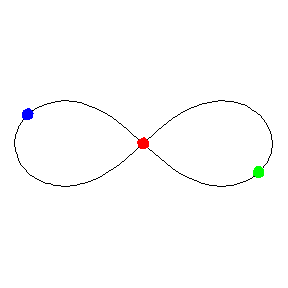
\includegraphics[max width=0.65\linewidth]{../images/cris-moore-figure8.png}\]
Also see:

\begin{enumerate}
\def\labelenumi{\arabic{enumi})}
\setcounter{enumi}{4}
\tightlist
\item
  Richard Montgomery, ``The \(N\)-body problem, the braid group, and
  action-minimizing periodic solutions'', \emph{Nonlinearity}
  \textbf{11} (1998), 363--371. Also available at
  \texttt{http://count.ucsc.edu/\textasciitilde{}rmont/papers/NbdyBraids.pdf}
\end{enumerate}

There is also the issue of whether a particle can shoot off to infinity
in a finite amount of time. Of course this isn't possible in the real
world, but Newtonian physics has no ``speed limit'', and we're
idealizing our particles as points. So, if two or more of them get
arbitrarily close to each other, the potential energy they liberate
could in principle give another particle enough kinetic energy to zip
off to infinity! Then our solution becomes undefined after a finite
amount of time.

Zhihong Xia showed this can actually happen in the \(N\)-body problem
for \(N = 5\) or bigger:

\begin{enumerate}
\def\labelenumi{\arabic{enumi})}
\setcounter{enumi}{5}
\tightlist
\item
  Zhihong Xia, ``The existence of non-collision singularities in
  Newtonian systems'', \emph{Ann. Math.} \textbf{135} (1992), 411--468.
\end{enumerate}

or for a more popular account:

\begin{enumerate}
\def\labelenumi{\arabic{enumi})}
\setcounter{enumi}{6}
\tightlist
\item
  Donald G. Saari and Zhihong Xia, ``Off to infinity in finite time'',
  \emph{AMS Notices} (May 1995), 538--546. Also available at
  \texttt{http://www.ams.org/notices/199505/saari-2.pdf}
\end{enumerate}

As far as I know, the question is still open for \(N = 4\). Another
question concerns how \emph{likely} it is for our solution to become
undefined in a finite amount of time. If it's infinitely improbable, we
say we have ``asymptotic completeness'' for the \(N\)-body problem. I
seem to recall that the \(N\)-body problem has been shown asymptotically
complete for \(N = 3\), but not higher \(N\).

Now --- back to my tale of Lie groups and geometry!

So far I've talked about how to any complex simple Lie group \(G\) we
can associate an ``incidence geometry'': a generalization of projective
geometry having \(G\) as its symmetry group. Each different type of
``figure'' in this geometry corresponds to a dot in the Dynkin diagram
for \(G\). For example, when \(G = \mathrm{SL}(4,\mathbb{C})\) we have
\[
  \begin{tikzpicture}
    \node[label=below:{points}] at (0,0) {$\bullet$};
    \node[label=below:{lines}] at (2,0) {$\bullet$};
    \node[label=below:{planes}] at (4,0) {$\bullet$};
    \draw[thick] (0,0) to (4,0);
  \end{tikzpicture}
\] For each dot, the space of all figures of the corresponding type is
called a ``Grassmannian'', and it's a manifold of the form G/P, where P
is a ``maximal parabolic'' subgroup of G.

More generally, any subset of dots in the Dynkin diagram corresponds to
a type of ``flag''. A flag is a collection of figures satisfying certain
incidence relations. For example, this subset: \[
  \begin{tikzpicture}
    \node[label=below:{points}] at (0,0) {$\times$};
    \node[label=below:{lines}] at (2,0) {$\bullet$};
    \node[label=below:{planes}] at (4,0) {$\times$};
    \draw[thick] (0,0) to (4,0);
  \end{tikzpicture}
\] corresponds to the type of flag consisting of a point lying on a
plane. The space of all flags of a particular type is called a ``flag
manifold'', and it's a manifold of the form \(G/P\), where \(P\) is a
``parabolic'' subgroup of \(G\).

I also said a bit about how we can quantize this entire story! This is
actually what got me interested in this whole business. In loop quantum
gravity we run around claiming that space is made of quantum triangles,
quantum tetrahedra and the like --- see
\protect\hyperlink{week113}{``Week 113''} and
\protect\hyperlink{week134}{``Week 134''} if you don't believe me. The
whole theory emerges naturally from the way Euclidean and Lorentzian
geometry are related to representations of the rotation and Lorentz
groups, but it got me wondering how the story would change if we changed
the group to something fancier --- as we might in a theory that tried to
unify gravity with other forces, for example. So I started studying
incidence geometry and group representations, and wound up learning lots
of math so beautiful that it has, so far, completely sidetracked me from
my original goal! I'll get back to it eventually\ldots.

Anyway, let me say more about this quantum aspect now. This is the royal
road to understanding representations of simple Lie groups. For
starters, fix a complex simple Lie group \(G\) and any parabolic
subgroup \(P\). Since \(G\) and \(P\) are complex Lie groups, the flag
manifold \(G/P\) is a complex manifold. More precisely, it has a complex
structure that is invariant under the action of \(G\).

On the other hand, we can write the flag manifold as \(K/L\), where
\(K\) is the maximal compact subgroup of \(G\), and \(L\) is the
intersection of \(K\) and \(P - L\) is called a ``Levi subgroup''. Since
\(K\) is compact, we can take any Riemannian metric on the flag manifold
and average it with respect to the action of \(K\) to get a Riemannian
metric that is invariant under the action of \(K\).

So, the flag manifold has a complex structure and metric that are both
invariant under \(K\)!

If this doesn't thrill you, consider the simplest example: \[
  \begin{aligned}
    G &= \mathrm{SL}(2,\mathbb{C})
  \\K &= \mathrm{SU}(2)
  \\P &= \{\mbox{upper triangular matrices in $\mathrm{SL}(2,\mathbb{C})$}\}
  \\L &= \{\mbox{diagonal matrices in $\mathrm{SL}(2,\mathbb{C})$}\}
  \end{aligned}
\] Here \(G/P = K/L\) is a \(2\)-sphere, the complex structure is the
usual way of thinking of this as the Riemann sphere, and the metric can
be any multiple of the usual round metric on the sphere. The complex
structure is invariant under all of \(G = \mathrm{SL}(2,\mathbb{C})\).
That's why \(\mathrm{SL}(2,\mathbb{C})\) is the double cover of the
group of conformal transformations of the Riemann sphere! The metric is
only invariant under \(K = \mathrm{SU}(2)\). That's why
\(\mathrm{SU}(2)\) is the double cover of the group of rotations of the
sphere!

All this stuff is wonderfully important in physics --- especially since
\(\mathrm{SL}(2,\mathbb{C})\) is also the double cover of the Lorentz
group, and the Riemann sphere is also the ``heavenly sphere'' upon which
we see the distant stars. I have already lavished attention on this
network of ideas in \protect\hyperlink{week162}{``Week 162''}\ldots{}
but what we're engaged in now is generalizing it to \emph{arbitrary}
complex simple Lie groups!

Now, a basic principle of geometry is that any two of the following
structures on a manifold determine the third \emph{if} they satisfy a
certain compatibility condition:

\begin{itemize}
\tightlist
\item
  complex structure \(J\)
\item
  Riemannian metric \(g\)
\item
  symplectic structure \(w\)
\end{itemize}

and in this case we get a ``Kaehler manifold'': a manifold with a
complex structure \(J\) and a complex inner product on the tangent
vectors whose real part is \(g\) and whose imaginary part is \(w\).

Furthermore, one of the big facts of quantization is that while the
phase space of a classical system is a symplectic manifold, we can only
quantize it and get a Hilbert space if we equip it with some extra
structure\ldots{} for example, by making it into a Kaehler manifold!
Once the phase space is a Kaehler manifold, we can look for a complex
line bundle over it with a connection whose curvature is the symplectic
structure. If this bundle exists, it's essentially unique, and we can
take the space of its holomorphic sections to be the Hilbert space of
states of the \emph{quantum} version of our system. For details, try my
webpage on geometric quantization, or these books, listed in rough order
of increasing difficulty and depth:

\begin{enumerate}
\def\labelenumi{\arabic{enumi})}
\setcounter{enumi}{7}
\item
  John Baez, ``Geometric quantization'',
  \texttt{http://math.ucr.edu/home/baez/quantization.html}
\item
  J. Snyatycki, \emph{Geometric Quantization and Quantum Mechanics},
  Springer-Verlag, New York, 1980.
\item
  Nicholas Woodhouse, \emph{Geometric Quantization}, Oxford U. Press,
  Oxford, 1992.
\item
  Norman E. Hurt, \emph{Geometric Quantization in Action: Applications
  of Harmonic Analysis in Quantum Statistical Mechanics and Quantum
  Field Theory}, Kluwer, Boston, 1983.
\end{enumerate}

In the beautiful situation I'm discussing now, the math gods are kind:
the complex structure and metric on the flag manifold fit together to
make it into a Kaehler manifold, so we can quantize it and get a Hilbert
space. And since everything in sight is invariant under the group K, our
Hilbert space becomes a unitary representation of K. This rep turns out
to be irreducible\ldots{} and we get all the unitary irreps of compact
simple Lie groups this way!

By easy abstract nonsense, the unitary irreps of \(K\) are also all the
finite-dimensional irreps of \(G\). So, we've just conquered a great
deal of territory in the land of group representations. You may have
seen other ways to get all the irreps of simple Lie groups: for example,
``heighest-weight representations'' or ``geometric quantization of
coadjoint orbits''. In fact, all these tricks are secretly just
different ways of talking about the same thing. It took me years to
learn this secret, but it's yours for free!

However, there are some small subtleties we shouldn't sweep under the
rug. We've seen that our flag manifold has a god-given complex
structure, but it usually has \emph{lots} of \(K\)-invariant metrics,
since we could take \emph{any} metric and average it with respect to the
action of \(K\). So, there are lots of \(K\)-invariant Kaehler
structures on our flag manifold.

How many are there? Well, I said that we get a flag manifold from any
subset of the dots in the Dynkin diagram for \(G\). It turns out that
\(K\)-invariant Kaehler structure on this flag manifold correspond to
ways of labelling the dots in this subset with positive real numbers.
And we can geometrically quantize the flag manifold to get an irrep of
\(G\) precisely when these numbers are \emph{integers!}

The simplest situation is when our flag manifold is a Grassmannian. This
corresponds to a single dot in the Dynkin diagram. If we label this dot
with the number \(1\), we get a so-called ``fundamental representation''
of our group. I sketched in \protect\hyperlink{week180}{``Week 180''}
how to get all the other irreps from these.

Now let me illustrate all this stuff by going through all the classical
series of simple Lie groups and seeing what we get.

\begin{itemize}
\item
  \(\mathrm{A}_n\): Here are the Grassmannians for some of the
  \(\mathrm{A}_n\) series, that is, the groups
  \(\mathrm{SL}(n+1,\mathbb{C})\). I've drawn the Dynkin diagrams with
  each dot labelled by the corresponding type of geometrical figure and
  the dimension of the Grassmannian of all figures of this type. We can
  think of these figures as vector subspaces of \(\mathbb{C}^{n+1}\). We
  can also think of them as spaces of one less dimension in
  \(\mathbb{CP}^n\). Either way, we are talking about \emph{projective}
  geometry: \[
      \begin{tikzpicture}[xscale=0.95,yscale=1.6]
        \node[label=below:{\scriptsize$1$},label=above:{\scriptsize 1d subspaces}] at (0,0) {$\bullet$};
        \node[label=below:{\scriptsize$2$},label=above:{\scriptsize 1d subspaces}] at (-1,-1) {$\bullet$};
        \node[label=below:{\scriptsize$2$},label=above:{\scriptsize 2d subspaces}] at (1,-1) {$\bullet$};
        \node[label=below:{\scriptsize$3$},label=above:{\scriptsize 1d subspaces}] at (-2,-2) {$\bullet$};
        \node[label=below:{\scriptsize$4$},label=above:{\scriptsize 2d subspaces}] at (0,-2) {$\bullet$};
        \node[label=below:{\scriptsize$3$},label=above:{\scriptsize 3d subspaces}] at (2,-2) {$\bullet$};
        \node[label=below:{\scriptsize$4$},label=above:{\scriptsize 1d subspaces}] at (-3,-3) {$\bullet$};
        \node[label=below:{\scriptsize$6$},label=above:{\scriptsize 2d subspaces}] at (-1,-3) {$\bullet$};
        \node[label=below:{\scriptsize$6$},label=above:{\scriptsize 3d subspaces}] at (1,-3) {$\bullet$};
        \node[label=below:{\scriptsize$4$},label=above:{\scriptsize 4d subspaces}] at (3,-3) {$\bullet$};
        %
        \draw[thick] (-1,-1) to (1,-1);
        \draw[thick] (-2,-2) to (2,-2);
        \draw[thick] (-3,-3) to (3,-3);
        %
        \node at (-5.5,0) {$\mathrm{A}_1$: $\mathrm{SL}(2,\mathbb{C})$};
        \node at (-5.5,-1) {$\mathrm{A}_2$: $\mathrm{SL}(3,\mathbb{C})$};
        \node at (-5.5,-2) {$\mathrm{A}_3$: $\mathrm{SL}(4,\mathbb{C})$};
        \node at (-5.5,-3) {$\mathrm{A}_4$: $\mathrm{SL}(5,\mathbb{C})$};
      \end{tikzpicture}
    \] Recognize the numbers labelling the Dynkin diagram dots? It's a
  weird modified version of Pascal's triangle --- but can you figure out
  the pattern?

  No? I claim you learned this table of numbers when you were in grade
  school: just tilt your head 45 degrees and you'll recognize it!

  Next, here's what we get from quantizing these Grassmannians. I've
  labelled each dot by the name of the corresponding fundamental
  representation and its dimension. All these reps are exterior powers
  of the obvious rep of \(\mathrm{SL}(n+1,\mathbb{C})\) on
  \(\mathbb{C}^{n+1}\). We call elements of the \(p\)th exterior power
  ``\(p\)-vectors'', or ``multivectors'' in general: \[
      \begin{tikzpicture}[xscale=0.95,yscale=1.6]
        \node[label=below:{\scriptsize$2$},label=above:{\scriptsize vectors}] at (0,0) {$\bullet$};
        \node[label=below:{\scriptsize$3$},label=above:{\scriptsize vectors}] at (-1,-1) {$\bullet$};
        \node[label=below:{\scriptsize$3$},label=above:{\scriptsize bivectors}] at (1,-1) {$\bullet$};
        \node[label=below:{\scriptsize$4$},label=above:{\scriptsize vectors}] at (-2,-2) {$\bullet$};
        \node[label=below:{\scriptsize$6$},label=above:{\scriptsize bivectors}] at (0,-2) {$\bullet$};
        \node[label=below:{\scriptsize$4$},label=above:{\scriptsize 3-vectors}] at (2,-2) {$\bullet$};
        \node[label=below:{\scriptsize$5$},label=above:{\scriptsize vectors}] at (-3,-3) {$\bullet$};
        \node[label=below:{\scriptsize$10$},label=above:{\scriptsize bivectors}] at (-1,-3) {$\bullet$};
        \node[label=below:{\scriptsize$10$},label=above:{\scriptsize 3-vectors}] at (1,-3) {$\bullet$};
        \node[label=below:{\scriptsize$5$},label=above:{\scriptsize 4-vectors}] at (3,-3) {$\bullet$};
        %
        \draw[thick] (-1,-1) to (1,-1);
        \draw[thick] (-2,-2) to (2,-2);
        \draw[thick] (-3,-3) to (3,-3);
        %
        \node at (-5.5,0) {$\mathrm{A}_1$: $\mathrm{SL}(2,\mathbb{C})$};
        \node at (-5.5,-1) {$\mathrm{A}_2$: $\mathrm{SL}(3,\mathbb{C})$};
        \node at (-5.5,-2) {$\mathrm{A}_3$: $\mathrm{SL}(4,\mathbb{C})$};
        \node at (-5.5,-3) {$\mathrm{A}_4$: $\mathrm{SL}(5,\mathbb{C})$};
      \end{tikzpicture}
    \] Here the numbers labelling the dots form Pascal's triangle! So we
  see that Pascal's triangle is a quantized version of the
  multiplication table. (That was the answer to the previous puzzle, by
  the way --- our triangle was just the multiplication table viewed from
  a funny angle.)
\item
  \(\mathrm{B}_n\): Next let's look at the \(\mathrm{B}_n\) series.
  \(\mathrm{B}_n\) is another name for the complexified rotation group
  \(\mathrm{SO}(2n+1,\mathbb{C})\), or if you prefer, its double cover
  \(\mathrm{Spin}(2n+1,\mathbb{C})\). A Grassmannian for this group is a
  space consisting of all \(p\)-dimensional ``isotropic'' subspaces of
  \(\mathbb{C}^{2n+1}\) --- that is, subspaces on which a nondegenerate
  symmetric bilinear form vanishes.

  As I explained in \protect\hyperlink{week180}{``Week 180''}, these
  Grassmannians show up when we study relativity in odd-dimensional
  Minkowski spacetime, especially when we complexify and compactify.
  Another way to put it is that this is all about \emph{conformal}
  geometry in odd dimensions! We've already seen that conformal geometry
  in even dimensions is very different, and we'll get to that later.

  Here are the Grassmannians and their dimensions: \[
      \begin{tikzpicture}[xscale=0.95,yscale=1.6]
        \draw[double,double equal sign distance] (0,-1) to (1,-1);
        \draw[double,double equal sign distance,-implies] (-1,-1) to (0.05,-1);
        \draw[thick] (-2,-2) to (0,-2);
        \draw[double,double equal sign distance] (1,-2) to (2,-2);
        \draw[double,double equal sign distance,-implies] (0,-2) to (1.05,-2);
        \draw[thick] (-3,-3) to (1,-3);
        \draw[double,double equal sign distance] (2,-3) to (3,-3);
        \draw[double,double equal sign distance,-implies] (1,-3) to (2.05,-3);
        %
        \node[label=below:{\scriptsize$1$},label={[label distance=1mm]above:{\scriptsize isotropic}},label={[label distance=-2mm]above:{\scriptsize 1d subspaces}}] at (0,0) {$\bullet$};
        \node[label=below:{\scriptsize$3$},label={[label distance=1mm]above:{\scriptsize isotropic}},label={[label distance=-2mm]above:{\scriptsize 1d subspaces}}] at (-1,-1) {$\bullet$};
        \node[label=below:{\scriptsize$3$},label={[label distance=1mm]above:{\scriptsize isotropic}},label={[label distance=-2mm]above:{\scriptsize 2d subspaces}}] at (1,-1) {$\bullet$};
        \node[label=below:{\scriptsize$5$},label={[label distance=1mm]above:{\scriptsize isotropic}},label={[label distance=-2mm]above:{\scriptsize 1d subspaces}}] at (-2,-2) {$\bullet$};
        \node[label=below:{\scriptsize$7$},label={[label distance=1mm]above:{\scriptsize isotropic}},label={[label distance=-2mm]above:{\scriptsize 2d subspaces}}] at (0,-2) {$\bullet$};
        \node[label=below:{\scriptsize$6$},label={[label distance=1mm]above:{\scriptsize isotropic}},label={[label distance=-2mm]above:{\scriptsize 3d subspaces}}] at (2,-2) {$\bullet$};
        \node[label=below:{\scriptsize$7$},label={[label distance=1mm]above:{\scriptsize isotropic}},label={[label distance=-2mm]above:{\scriptsize 1d subspaces}}] at (-3,-3) {$\bullet$};
        \node[label=below:{\scriptsize$11$},label={[label distance=1mm]above:{\scriptsize isotropic}},label={[label distance=-2mm]above:{\scriptsize 2d subspaces}}] at (-1,-3) {$\bullet$};
        \node[label=below:{\scriptsize$12$},label={[label distance=1mm]above:{\scriptsize isotropic}},label={[label distance=-2mm]above:{\scriptsize 3d subspaces}}] at (1,-3) {$\bullet$};
        \node[label=below:{\scriptsize$10$},label={[label distance=1mm]above:{\scriptsize isotropic}},label={[label distance=-2mm]above:{\scriptsize 4d subspaces}}] at (3,-3) {$\bullet$};
        %
        \node at (-5.5,0) {$\mathrm{B}_1$: $\mathrm{Spin}(3,\mathbb{C})$};
        \node at (-5.5,-1) {$\mathrm{B}_2$: $\mathrm{Spin}(5,\mathbb{C})$};
        \node at (-5.5,-2) {$\mathrm{B}_3$: $\mathrm{Spin}(7,\mathbb{C})$};
        \node at (-5.5,-3) {$\mathrm{B}_4$: $\mathrm{Spin}(9,\mathbb{C})$};
      \end{tikzpicture}
    \] I'm sure these are well-known, but James Dolan and I had a lot of
  fun one evening working these out, using a lot of numerology that we
  eventually justified by a method I'll explain later.

  Here's a bigger chart of these dimensions: \[
      \begin{tikzpicture}[xscale=0.5,yscale=0.6]
        \node at (0,0) {$1$};
        \node at (-1,-1) {$3$};
        \node at (1,-1) {$3$};
        \node at (-2,-2) {$5$};
        \node at (0,-2) {$7$};
        \node at (2,-2) {$6$};
        \node at (-3,-3) {$7$};
        \node at (-1,-3) {$11$};
        \node at (1,-3) {$12$};
        \node at (3,-3) {$10$};
        \node at (-4,-4) {$9$};
        \node at (-2,-4) {$15$};
        \node at (0,-4) {$18$};
        \node at (2,-4) {$18$};
        \node at (4,-4) {$15$};
        \node at (-5,-5) {$11$};
        \node at (-3,-5) {$19$};
        \node at (-1,-5) {$24$};
        \node at (1,-5) {$26$};
        \node at (3,-5) {$25$};
        \node at (5,-5) {$21$};
        \node at (-6,-6) {$13$};
        \node at (-4,-6) {$23$};
        \node at (-2,-6) {$30$};
        \node at (0,-6) {$34$};
        \node at (2,-6) {$35$};
        \node at (4,-6) {$33$};
        \node at (6,-6) {$28$};
        \node at (-7,-7) {$15$};
        \node at (-5,-7) {$27$};
        \node at (-3,-7) {$36$};
        \node at (-1,-7) {$42$};
        \node at (1,-7) {$45$};
        \node at (3,-7) {$45$};
        \node at (5,-7) {$42$};
        \node at (7,-7) {$36$};
        %
        \node at (-9,0) {$\mathrm{B}_1$};
        \node at (-9,-1) {$\mathrm{B}_2$};
        \node at (-9,-2) {$\mathrm{B}_3$};
        \node at (-9,-3) {$\mathrm{B}_4$};
        \node at (-9,-4) {$\mathrm{B}_5$};
        \node at (-9,-5) {$\mathrm{B}_6$};
        \node at (-9,-6) {$\mathrm{B}_7$};
        \node at (-9,-7) {$\mathrm{B}_8$};
        \draw[thick,dashed] (-8,0.5) to (-8,-7.5);
      \end{tikzpicture}
    \] I leave it as an easy puzzle to figure out the pattern, and a
  harder puzzle to prove it's true. Don't be overly distracted by the
  symmetry lurking in rows 2, 5, and 8 --- every third row has this
  symmetry, but it's a bit of a red herring!

  If we quantize these Grassmannians we get these fundamental reps of
  \(\mathrm{Spin}(2n+1,\mathbb{C})\): \[
      \begin{tikzpicture}[xscale=0.95,yscale=1.6]
        \draw[double,double equal sign distance] (0,-1) to (1,-1);
        \draw[double,double equal sign distance,-implies] (-1,-1) to (0.05,-1);
        \draw[thick] (-2,-2) to (0,-2);
        \draw[double,double equal sign distance] (1,-2) to (2,-2);
        \draw[double,double equal sign distance,-implies] (0,-2) to (1.05,-2);
        \draw[thick] (-3,-3) to (1,-3);
        \draw[double,double equal sign distance] (2,-3) to (3,-3);
        \draw[double,double equal sign distance,-implies] (1,-3) to (2.05,-3);
        %
        \node[label=below:{\scriptsize$2$},label=above:{\scriptsize spinors}] at (0,0) {$\bullet$};
        \node[label=below:{\scriptsize$5$},label=above:{\scriptsize vectors}] at (-1,-1) {$\bullet$};
        \node[label=below:{\scriptsize$4$},label=above:{\scriptsize spinors}] at (1,-1) {$\bullet$};
        \node[label=below:{\scriptsize$7$},label=above:{\scriptsize vectors}] at (-2,-2) {$\bullet$};
        \node[label=below:{\scriptsize$21$},label=above:{\scriptsize bivectors}] at (0,-2) {$\bullet$};
        \node[label=below:{\scriptsize$8$},label=above:{\scriptsize spinors}] at (2,-2) {$\bullet$};
        \node[label=below:{\scriptsize$9$},label=above:{\scriptsize vectors}] at (-3,-3) {$\bullet$};
        \node[label=below:{\scriptsize$36$},label=above:{\scriptsize bivectors}] at (-1,-3) {$\bullet$};
        \node[label=below:{\scriptsize$84$},label=above:{\scriptsize 3-vectors}] at (1,-3) {$\bullet$};
        \node[label=below:{\scriptsize$16$},label=above:{\scriptsize spinors}] at (3,-3) {$\bullet$};
        %
        \node at (-5.5,0) {$\mathrm{B}_1$: $\mathrm{Spin}(3,\mathbb{C})$};
        \node at (-5.5,-1) {$\mathrm{B}_2$: $\mathrm{Spin}(5,\mathbb{C})$};
        \node at (-5.5,-2) {$\mathrm{B}_3$: $\mathrm{Spin}(7,\mathbb{C})$};
        \node at (-5.5,-3) {$\mathrm{B}_4$: $\mathrm{Spin}(9,\mathbb{C})$};
      \end{tikzpicture}
    \] As before, the dimension of the space of \(p\)-vectors in
  \(q\)-dimensional space comes straight from Pascal's triangle: it's
  \(q\) choose \(p\). But now we also have spinor reps; the dimensions
  of these are powers of 2.
\item
  \(\mathrm{C}_n\): Next let's look at the Grassmannians for the
  \(\mathrm{C}_n\) series, that is, the symplectic groups
  \(\mathrm{Sp}(2n,\mathbb{C})\). This is the only series of classical
  groups I haven't touched yet! Just as the \(\mathrm{A}_n\) series are
  symmetry groups of projective geometry and the \(\mathrm{B}_n\) and
  \(\mathrm{D}_n\) series are symmetry groups of conformal geometry, the
  \(\mathrm{C}_n\) series are symmetry groups of ``projective
  symplectic'' geometry. Unfortunately I don't know much about this
  subject --- at least not consciously. It should be important in
  physics, but I'm not sure where!

  Anyway, \(\mathrm{Sp}(2n,\mathbb{C})\) is the group of linear
  transformations of \(\mathbb{C}^{2n}\) that preserve a symplectic
  form: that is, a nondegenerate \emph{antisymmetric} bilinear form. A
  Grassmannian for this group again consists of all \(p\)-dimensional
  isotropic subspaces of \(\mathbb{C}^{2n}\), where now a subspace is
  ``isotropic'' if the symplectic form vanishes on it.

  Here's a little table of these Grassmannians: \[
      \begin{tikzpicture}[xscale=0.95,yscale=1.6]
        \draw[double,double equal sign distance] (-1,-1) to (0.05,-1);
        \draw[double,double equal sign distance,implies-] (-0.05,-1) to (1,-1);
        \draw[thick] (-2,-2) to (0,-2);
        \draw[double,double equal sign distance] (0,-2) to (1.05,-2);
        \draw[double,double equal sign distance,implies-] (0.95,-2) to (2,-2);
        \draw[thick] (-3,-3) to (1,-3);
        \draw[double,double equal sign distance] (1,-3) to (2.05,-3);
        \draw[double,double equal sign distance,implies-] (1.95,-3) to (3,-3);
        %
        \node[label=below:{\scriptsize$1$},label={[label distance=1mm]above:{\scriptsize isotropic}},label={[label distance=-2mm]above:{\scriptsize 1d subspaces}}] at (0,0) {$\bullet$};
        \node[label=below:{\scriptsize$3$},label={[label distance=1mm]above:{\scriptsize isotropic}},label={[label distance=-2mm]above:{\scriptsize 1d subspaces}}] at (-1,-1) {$\bullet$};
        \node[label=below:{\scriptsize$3$},label={[label distance=1mm]above:{\scriptsize isotropic}},label={[label distance=-2mm]above:{\scriptsize 2d subspaces}}] at (1,-1) {$\bullet$};
        \node[label=below:{\scriptsize$5$},label={[label distance=1mm]above:{\scriptsize isotropic}},label={[label distance=-2mm]above:{\scriptsize 1d subspaces}}] at (-2,-2) {$\bullet$};
        \node[label=below:{\scriptsize$7$},label={[label distance=1mm]above:{\scriptsize isotropic}},label={[label distance=-2mm]above:{\scriptsize 2d subspaces}}] at (0,-2) {$\bullet$};
        \node[label=below:{\scriptsize$6$},label={[label distance=1mm]above:{\scriptsize isotropic}},label={[label distance=-2mm]above:{\scriptsize 3d subspaces}}] at (2,-2) {$\bullet$};
        \node[label=below:{\scriptsize$7$},label={[label distance=1mm]above:{\scriptsize isotropic}},label={[label distance=-2mm]above:{\scriptsize 1d subspaces}}] at (-3,-3) {$\bullet$};
        \node[label=below:{\scriptsize$11$},label={[label distance=1mm]above:{\scriptsize isotropic}},label={[label distance=-2mm]above:{\scriptsize 2d subspaces}}] at (-1,-3) {$\bullet$};
        \node[label=below:{\scriptsize$12$},label={[label distance=1mm]above:{\scriptsize isotropic}},label={[label distance=-2mm]above:{\scriptsize 3d subspaces}}] at (1,-3) {$\bullet$};
        \node[label=below:{\scriptsize$10$},label={[label distance=1mm]above:{\scriptsize isotropic}},label={[label distance=-2mm]above:{\scriptsize 4d subspaces}}] at (3,-3) {$\bullet$};
        %
        \node at (-5.5,0) {$\mathrm{C}_1$: $\mathrm{Sp}(2,\mathbb{C})$};
        \node at (-5.5,-1) {$\mathrm{C}_2$: $\mathrm{Sp}(4,\mathbb{C})$};
        \node at (-5.5,-2) {$\mathrm{C}_3$: $\mathrm{Sp}(6,\mathbb{C})$};
        \node at (-5.5,-3) {$\mathrm{C}_4$: $\mathrm{Sp}(8,\mathbb{C})$};
      \end{tikzpicture}
    \] You'll notice the dimensions are the same as in the
  \(\mathrm{B}_n\) case! That's because their Dynkin diagrams are almost
  the same: for reasons I may someday explain, dimensions of flag
  manifolds don't care which way the little arrows on the Dynkin
  diagrams point, since they depend only on the \emph{reflection group}
  associated to this diagram (see \protect\hyperlink{week62}{``Week
  62''}).

  However, the dimensions of the fundamental representations are
  different from the \(\mathrm{B}_n\) case --- and I don't even know
  what they are! The basic idea is this: the space of \(p\)-vectors is
  no longer an irrep for \(\mathrm{Sp}(2n,\mathbb{C})\), but contracting
  with the symplectic form maps \(p\)-vectors to \((p-2)\)-vectors, and
  the kernel of this map is the \$p4th fundamental rep of
  \(\mathrm{Sp}(2n)\). Let's call these guys ``irreducible
  \(p\)-vectors''.

  Oh heck, I can \emph{guess} the dimensions of these guys from
  this\ldots{} I guess they're just the dimension of the \(p\)-vectors
  minus the dimension of the \((p-2)\)-vectors. Here's a table of these
  guesses: \[
      \begin{tikzpicture}[xscale=0.95,yscale=1.6]
        \draw[double,double equal sign distance] (-1,-1) to (0.05,-1);
        \draw[double,double equal sign distance,implies-] (-0.05,-1) to (1,-1);
        \draw[thick] (-2,-2) to (0,-2);
        \draw[double,double equal sign distance] (0,-2) to (1.05,-2);
        \draw[double,double equal sign distance,implies-] (0.95,-2) to (2,-2);
        \draw[thick] (-3,-3) to (1,-3);
        \draw[double,double equal sign distance] (1,-3) to (2.05,-3);
        \draw[double,double equal sign distance,implies-] (1.95,-3) to (3,-3);
        %
        \node[label=below:{\scriptsize$2$},label=above:{\scriptsize vectors}] at (0,0) {$\bullet$};
        \node[label=below:{\scriptsize$4$},label=above:{\scriptsize vectors}] at (-1,-1) {$\bullet$};
        \node[label=below:{\scriptsize$5$},label={[label distance=1mm]above:{\scriptsize irreducible}},label={[label distance=-1mm]above:{\scriptsize bivectors}}] at (1,-1) {$\bullet$};
        \node[label=below:{\scriptsize$6$},label=above:{\scriptsize vectors}] at (-2,-2) {$\bullet$};
        \node[label=below:{\scriptsize$14$},label={[label distance=1mm]above:{\scriptsize irreducible}},label={[label distance=-1mm]above:{\scriptsize bivectors}}] at (0,-2) {$\bullet$};
        \node[label=below:{\scriptsize$14$},label={[label distance=1mm]above:{\scriptsize irreducible}},label={[label distance=-1mm]above:{\scriptsize 3-vectors}}] at (2,-2) {$\bullet$};
        \node[label=below:{\scriptsize$8$},label=above:{\scriptsize vectors}] at (-3,-3) {$\bullet$};
        \node[label=below:{\scriptsize$27$},label={[label distance=1mm]above:{\scriptsize irreducible}},label={[label distance=-1mm]above:{\scriptsize bivectors}}] at (-1,-3) {$\bullet$};
        \node[label=below:{\scriptsize$48$},label={[label distance=1mm]above:{\scriptsize irreducible}},label={[label distance=-1mm]above:{\scriptsize 3-vectors}}] at (1,-3) {$\bullet$};
        \node[label=below:{\scriptsize$42$},label={[label distance=1mm]above:{\scriptsize irreducible}},label={[label distance=-1mm]above:{\scriptsize 4-vectors}}] at (3,-3) {$\bullet$};
        %
        \node at (-5.5,0) {$\mathrm{C}_1$: $\mathrm{Sp}(2,\mathbb{C})$};
        \node at (-5.5,-1) {$\mathrm{C}_2$: $\mathrm{Sp}(4,\mathbb{C})$};
        \node at (-5.5,-2) {$\mathrm{C}_3$: $\mathrm{Sp}(6,\mathbb{C})$};
        \node at (-5.5,-3) {$\mathrm{C}_4$: $\mathrm{Sp}(8,\mathbb{C})$};
      \end{tikzpicture}
    \] Maybe someone can tell if they're right.
\item
  \(\mathrm{D}_n\): Finally, \(\mathrm{D}_n\) is another name for the
  complexified rotation group \(\mathrm{SO}(2n,\mathbb{C})\) or its
  double cover \(\mathrm{Spin}(2n,\mathbb{C})\). The \(p\)th
  Grassmannian for this group consists of all \(p\)-dimensional
  isotropic subspaces of the space \(\mathbb{C}^{2n}\) equipped with a
  nondegenerate symmetric bilinear form --- \emph{except} for the
  top-dimensional Grassmannians, as I explained last week. These consist
  of self-dual or anti-self-dual subspaces. Self-duality is the special
  feature of conformal geometry in \emph{even} dimensions!

  Here are the Grassmannians and their dimensions: \[
      \begin{tikzpicture}[xscale=0.4,yscale=0.6]
        \node[label=above:{\scriptsize$1$},label=right:{\scriptsize self-dual 2d subspaces}] at (0,1) {$\bullet$};
        \node[label=below:{\scriptsize$1$},label=right:{\scriptsize anti-self-dual 2d subspaces}] at (0,-1) {$\bullet$};
        \node at (-8,0) {$\mathrm{D}_2$: $\mathrm{Spin}(4,\mathbb{C})$};
      \end{tikzpicture}
    \] \[
      \begin{tikzpicture}[xscale=0.4,yscale=0.6]
        \draw[thick] (0,1) to (-1,0) to (0,-1);
        \node[label=above:{\scriptsize$3$},label=right:{\scriptsize self-dual 3d subspaces}] at (0,1) {$\bullet$};
        \node[label=left:{\scriptsize$4$},label=right:{\scriptsize isotropic 1d subspaces}] at (-1,0) {$\bullet$};
        \node[label=below:{\scriptsize$3$},label=right:{\scriptsize anti-self-dual 3d subspaces}] at (0,-1) {$\bullet$};
        \node at (-8,0) {$\mathrm{D}_3$: $\mathrm{Spin}(6,\mathbb{C})$};
      \end{tikzpicture}
    \] \[
      \begin{tikzpicture}[xscale=0.4,yscale=0.6]
        \draw[thick] (0,1) to (-1,0) to (0,-1);
        \draw[thick] (-1,0) to (-4,0);
        \node[label=above:{\scriptsize$6$},label=right:{\scriptsize self-dual 4d subspaces}] at (0,1) {$\bullet$};
        \node[label={[label distance=-2mm]below left:{\scriptsize$9$}},label=right:{\scriptsize isotropic 2d subspaces}] at (-1,0) {$\bullet$};
        \node[label={below:{\scriptsize$6$}},label={[label distance=1mm]above:{\scriptsize isotropic}},label={[label distance=-2mm]above:{\scriptsize 1d subspaces}}] at (-4,0) {$\bullet$};
        \node[label=below:{\scriptsize$6$},label=right:{\scriptsize anti-self-dual 4d subspaces}] at (0,-1) {$\bullet$};
        \node at (-12,0) {$\mathrm{D}_4$: $\mathrm{Spin}(8,\mathbb{C})$};
      \end{tikzpicture}
    \] \[
      \begin{tikzpicture}[xscale=0.6,yscale=0.6]
        \draw[thick] (0,1) to (-1,0) to (0,-1);
        \draw[thick] (-1,0) to (-7,0);
        \node[label=above:{\scriptsize$10$},label=right:{\scriptsize self-dual 5d subspaces}] at (0,1) {$\bullet$};
        \node[label={[label distance=-2mm]below left:{\scriptsize$15$}},label=right:{\scriptsize isotropic 3d subspaces}] at (-1,0) {$\bullet$};
        \node[label={below:{\scriptsize$13$}},label=above:{\scriptsize 2d subspaces}] at (-4,0) {$\bullet$};
        \node[label={below:{\scriptsize$8$}},label=above:{\scriptsize 1d subspaces}] at (-7,0) {$\bullet$};
        \node[label=below:{\scriptsize$10$},label=right:{\scriptsize anti-self-dual 5d subspaces}] at (0,-1) {$\bullet$};
        \node at (-12,0) {$\mathrm{D}_5$: $\mathrm{Spin}(10,\mathbb{C})$};
      \end{tikzpicture}
    \] You'll notice that the numbers on the ``fishtails'' are
  triangular numbers: \(1, 3, 6, 10\ldots\) I'll say more later about
  how to calculate the rest of these numbers.

  As explained last week, the fundamental reps of the \(\mathrm{D}_n\)
  consist of \(p\)-vectors, except for those at the fishtails, which are
  left- and right-handed spinor reps: \[
      \begin{tikzpicture}[xscale=0.4,yscale=0.6]
        \node[label=above:{\scriptsize$2$},label=right:{\scriptsize left-handed spinors}] at (0,1) {$\bullet$};
        \node[label=below:{\scriptsize$2$},label=right:{\scriptsize right-handed spinors}] at (0,-1) {$\bullet$};
        \node at (-8,0) {$\mathrm{D}_2$: $\mathrm{Spin}(4,\mathbb{C})$};
      \end{tikzpicture}
    \] \[
      \begin{tikzpicture}[xscale=0.4,yscale=0.6]
        \draw[thick] (0,1) to (-1,0) to (0,-1);
        \node[label=above:{\scriptsize$4$},label=right:{\scriptsize left-handed spinors}] at (0,1) {$\bullet$};
        \node[label=left:{\scriptsize$6$},label=right:{\scriptsize vectors}] at (-1,0) {$\bullet$};
        \node[label=below:{\scriptsize$4$},label=right:{\scriptsize right-handed spinors}] at (0,-1) {$\bullet$};
        \node at (-8,0) {$\mathrm{D}_3$: $\mathrm{Spin}(6,\mathbb{C})$};
      \end{tikzpicture}
    \] \[
      \begin{tikzpicture}[xscale=0.4,yscale=0.6]
        \draw[thick] (0,1) to (-1,0) to (0,-1);
        \draw[thick] (-1,0) to (-4,0);
        \node[label=above:{\scriptsize$8$},label=right:{\scriptsize left-handed spinors}] at (0,1) {$\bullet$};
        \node[label={[label distance=-2mm]below left:{\scriptsize$28$}},label=right:{\scriptsize bivectors}] at (-1,0) {$\bullet$};
        \node[label={below:{\scriptsize$8$}},label=above:{\scriptsize vectors}] at (-4,0) {$\bullet$};
        \node[label=below:{\scriptsize$8$},label=right:{\scriptsize right-handed spinors}] at (0,-1) {$\bullet$};
        \node at (-12,0) {$\mathrm{D}_4$: $\mathrm{Spin}(8,\mathbb{C})$};
      \end{tikzpicture}
    \] \[
      \begin{tikzpicture}[xscale=0.4,yscale=0.6]
        \draw[thick] (0,1) to (-1,0) to (0,-1);
        \draw[thick] (-1,0) to (-7,0);
        \node[label=above:{\scriptsize$16$},label=right:{\scriptsize left-handed spinors}] at (0,1) {$\bullet$};
        \node[label={[label distance=-2mm]below left:{\scriptsize$120$}},label=right:{\scriptsize 3-vectors}] at (-1,0) {$\bullet$};
        \node[label={below:{\scriptsize$45$}},label=above:{\scriptsize bivectors}] at (-4,0) {$\bullet$};
        \node[label={below:{\scriptsize$10$}},label=above:{\scriptsize vectors}] at (-7,0) {$\bullet$};
        \node[label=below:{\scriptsize$16$},label=right:{\scriptsize right-handed spinors}] at (0,-1) {$\bullet$};
        \node at (-12,0) {$\mathrm{D}_5$: $\mathrm{Spin}(10,\mathbb{C})$};
      \end{tikzpicture}
    \] Again the dimension of the space of \(p\)-vectors in
  \(q\)-dimensional space comes from Pascal's triangle, while the
  dimensions of the spinor reps are powers of 2.
\end{itemize}

Let me conclude by listing the dimensions of Grassmannians for the
exceptional groups, as computed by James Dolan. I strongly doubt he's
the first to have computed these --- at this stage we're mainly learning
and reinventing known stuff --- but he did it using a nice trick I'd
like to mention. I was shocked at how unfamiliar these numbers were to
me, because all these Grassmannians should be definable using the
octonions: \[
  \begin{tikzpicture}
    \draw[double,double equal sign distance] (0,0) to (1,0);
    \draw[double,double equal sign distance,-implies] (0,0) to (0.55,0);
    \draw (0,0) to (1,0);
    \node[label=left:{$5$}] at (0,0) {$\bullet$};
    \node[label=right:{$5$}] at (1,0) {$\bullet$};
    \node at (-2,0) {$\mathrm{G}_2$};
  \end{tikzpicture}
\] \[
  \begin{tikzpicture}
    \draw[thick] (0,0) to (1,0);
    \draw[double,double equal sign distance] (1,0) to (2,0);
    \draw[double,double equal sign distance,-implies] (1,0) to (1.55,0);
    \draw[thick] (2,0) to (3,0);
    \node[label=below:{$43$}] at (0,0) {$\bullet$};
    \node[label=below:{$48$}] at (1,0) {$\bullet$};
    \node[label=below:{$48$}] at (2,0) {$\bullet$};
    \node[label=below:{$43$}] at (3,0) {$\bullet$};
    \node at (-2,0) {$\mathrm{F}_4$};
  \end{tikzpicture}
\] \[
  \begin{tikzpicture}
    \draw[thick] (0,0) to (4,0);
    \draw[thick] (2,0) to (2,1);
    \node[label=below:{$16$}] at (0,0) {$\bullet$};
    \node[label=below:{$25$}] at (1,0) {$\bullet$};
    \node[label=below:{$29$}] at (2,0) {$\bullet$};
    \node[label=above:{$21$}] at (2,1) {$\bullet$};
    \node[label=below:{$25$}] at (3,0) {$\bullet$};
    \node[label=below:{$16$}] at (4,0) {$\bullet$};
    \node at (-2,0) {$\mathrm{E}_6$};
  \end{tikzpicture}
\] \[
  \begin{tikzpicture}
    \draw[thick] (0,0) to (5,0);
    \draw[thick] (2,0) to (2,1);
    \node[label=below:{$33$}] at (0,0) {$\bullet$};
    \node[label=below:{$47$}] at (1,0) {$\bullet$};
    \node[label=below:{$53$}] at (2,0) {$\bullet$};
    \node[label=above:{$42$}] at (2,1) {$\bullet$};
    \node[label=below:{$50$}] at (3,0) {$\bullet$};
    \node[label=below:{$42$}] at (4,0) {$\bullet$};
    \node[label=below:{$27$}] at (5,0) {$\bullet$};
    \node at (-2,0) {$\mathrm{E}_7$};
  \end{tikzpicture}
\] \[
  \begin{tikzpicture}
    \draw[thick] (0,0) to (6,0);
    \draw[thick] (2,0) to (2,1);
    \node[label=below:{$78$}] at (0,0) {$\bullet$};
    \node[label=below:{$98$}] at (1,0) {$\bullet$};
    \node[label=below:{$106$}] at (2,0) {$\bullet$};
    \node[label=above:{$92$}] at (2,1) {$\bullet$};
    \node[label=below:{$104$}] at (3,0) {$\bullet$};
    \node[label=below:{$99$}] at (4,0) {$\bullet$};
    \node[label=below:{$83$}] at (5,0) {$\bullet$};
    \node[label=below:{$57$}] at (6,0) {$\bullet$};
    \node at (-2,0) {$\mathrm{E}_8$};
  \end{tikzpicture}
\]

You can calculate dimensions of these and all the other Grassmannians
for simple Lie groups by the following easy trick. Given the Dynkin
diagram for \(G\) and a chosen dot in it, remove this dot to get one or
more Dynkin diagrams for groups \(G_i\). Work out the dimension of the
space of maximal flags for \(G\), and subtract all the dimensions of the
spaces of maximal flags for the \(G_i\). Voila! You get the dimensions
of the Grassmannian corresponding to the \(i\)th dot.

The dimensions of maximal flag manifold for \(G\) is easy to compute, in
turn, because it's just \(\dim(G) - \dim(B)\), where \(B\) is the Borel.
And dimension of the Borel is just \((\dim(G) + \dim(T))/2\), where
\(T\) is the maximal torus, so that \(\dim(T)\) is the number of dots in
the Dynkin diagram.

\begin{center}\rule{0.5\linewidth}{0.5pt}\end{center}

\begin{quote}
\emph{Mathematics is the part of physics where experiments are cheap.}

--- V. I. Arnold,
\href{http://pauli.uni-muenster.de/~munsteg/arnold.html}{On teaching
mathematics}
\end{quote}



\hypertarget{week182}{%
\section{June 19, 2002}\label{week182}}

It's been a long time, but in the last Week's Finds I was telling you
about my adventures this spring in northern California, and I hadn't
quite gotten around to telling you about that cool conference on
``Nonabelian Hodge Theory'' at the MSRI in Berkeley. I'll continue my
story about that now\ldots{}

\ldots but first, a little detour through the Nile valley!

Egyptians liked to write fractions as the sum of reciprocals of
integers. For example, instead of writing \[\frac56\] those folks would
write something like \[\frac12 + \frac13\] Nobody is sure why, but one
possibility is that they started with a neat notation for \(1/n\), and
then wanted to extend this to handle other fractions, and couldn't think
of anything better.

Of course they \emph{could} have written \(m/n\) as
\[\underbrace{\frac1n+\ldots+\frac1n}_{\mbox{$m$ terms}}\] but they
preferred to use as few terms as possible. This leads to some tricky
questions. For example: clearly every fraction of the form \(4/n\) can
be written using 4 terms --- but can you always make do with just 3?
Nobody knows! This is called the Erdos-Strauss conjecture. Alan Swett
claims to have shown you only need 3 terms if \(n\) is less than or
equal to \(10^{14}\). For example:
\[\frac{4}{8689} = \frac{1}{2175} + \frac{1}{1718250} + \frac{1}{14929874250}.\]
For much more on this, see:

\begin{enumerate}
\def\labelenumi{\arabic{enumi})}
\item
  David Eppstein, ``Egyptian fractions'',
  \texttt{http://www.ics.uci.edu/\textasciitilde{}eppstein/numth/egypt/}
\item
  Alan Swett, ``The Erdos-Strauss conjecture'',
  \texttt{http://math.uindy.edu/swett/esc.htm}
\end{enumerate}

Egyptian fraction problems have a spooky way of showing up in various
unrelated mathematical contexts\ldots{} which have a spooky way of
turning out not to be unrelated after all!

For example, suppose we are trying to classify all the Platonic solids.
We're looking for ways to tile the surface of a sphere with regular
\(n\)-gons, with \(m\) meeting at each vertex. Suppose there is a total
of \(V\) vertices, \(E\) edges, and \(F\) faces. Since the Euler
characteristic of the sphere is \(2\), we have \[V - E + F = 2.\] Since
each face has \(n\) edges but 2 faces meet along each edge, we have
\[nF = 2E.\] Since each vertex has \(m\) edges meeting it but each edge
meets 2 vertices, we also have \[mV = 2E.\] Putting these equations
together we get \[2E\left(\frac1n + \frac1m - \frac12\right) = 2\] or
\[\frac1n + \frac1m = \frac12 + \frac1E.\] An Egyptian fractions
problem! It's obvious that this can only have solutions if
\(1/n + 1/m > 1/2\). And interestingly, all the solutions of this
inequality do indeed correspond to Platonic solids\ldots{} at least if
\(n,m > 2\). Here they are:

\begin{longtable}[]{@{}ll@{}}
\toprule
\((n,m)\) & Platonic solid\tabularnewline
\midrule
\endhead
\((3,3)\) & tetrahedron\tabularnewline
\((3,4)\) & octahedron\tabularnewline
\((4,3)\) & cube\tabularnewline
\((3,5)\) & icosahedron\tabularnewline
\((5,3)\) & dodecahedron\tabularnewline
\bottomrule
\end{longtable}

The cases \(n = 1,2\) don't give Platonic solids in the usual sense:
after all, most people don't like polygons to have just 1 or 2 edges.
Neither do the cases \(m = 1,2\), since most people don't like polyhedra
to have just 1 or 2 faces meeting at a vertex!

One can argue about whether these are irrational prejudices. But it's
actually good to study \emph{all} unordered pairs of natural numbers
with \[\frac1n + \frac1m > \frac12\] since they correspond to \emph{all}
the isomorphism classes of finite subgroups of the rotation group! The
Platonic solids have their symmetry groups, which don't change when we
switch \(n\) and \(m\). The solution \((n,1)\) corresponds to the cyclic
group \(\mathbb{Z}_n\): the symmetries of a regular \(n\)-gon, where
you're not allowed to flip it over. The solution \((n,2)\) corresponds
to the dihedral group \(D_n\): the symmetries of a regular n-gon where
you \emph{are} allowed to flip it over.

In some weird sense, maybe we should think of \(\mathbb{Z}_n\) and
\(D_n\) as the symmetry groups of Platonic solids with only 1 or 2
faces. I'll leave you to ponder the Platonic solids with only 1 or 2
vertices. If you get stuck, look up the word ``hosohedron''!

The story gets better if we also consider solutions of
\[\frac1n + \frac1m = \frac12\] which formally correspond to Platonic
solids where the number \(E\) of edges is infinite. In fact, these
correspond to tilings of the plane by regular polygons:

\begin{longtable}[]{@{}ll@{}}
\toprule
\((n,m)\) & tilings of the plane by\ldots{}\tabularnewline
\midrule
\endhead
\((3,6)\) & regular triangles\tabularnewline
\((6,3)\) & regular hexagons\tabularnewline
\((4,4)\) & (regular) squares\tabularnewline
\bottomrule
\end{longtable}

Similarly, solutions of \[\frac1n + \frac1m < \frac12\] give tilings of
the hyperbolic plane. For example, Escher used \((n,m) = (6,4)\) in some
of his prints, like this:
\[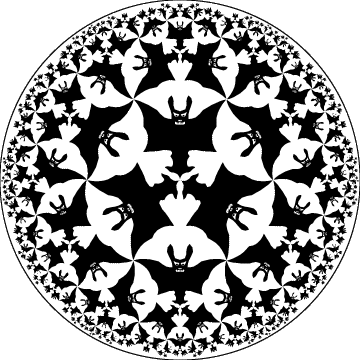
\includegraphics[scale=0.68]{../images/escher.png}\]

Let me try to arrange all this information in a table, using lines to
separate the spherical, planar and hyperbolic regions: \[
  \begin{tikzpicture}
    \matrix[
      column sep=.2cm,row sep=.1cm,
      nodes={text height=0.65cm},
    ]{
      \node{${}_m\backslash^n$}; & \node{$1$}; & \node{$2$}; & \node{$3$}; & \node{$4$}; & \node{$5$}; & \node{$6$}; & \node{$7$};\\
      \node{$1$}; & \node{$\mathbb{Z}_1$}; & \node{$\mathbb{Z}_2$}; & \node{$\mathbb{Z}_3$}; & \node{$\mathbb{Z}_4$}; & \node{$\mathbb{Z}_5$}; & \node{$\mathbb{Z}_6$}; & \node{$\mathbb{Z}_7$};\\
      \node{$2$}; & \node{$\mathbb{Z}_2$}; & \node{$\mathrm{D}_2$}; & \node{$\mathrm{D}_3$}; & \node{$\mathrm{D}_4$}; & \node{$\mathrm{D}_5$}; & \node{$\mathrm{D}_6$}; & \node{$\mathrm{D}_7$};\\
      \node{$3$}; & \node{$\mathbb{Z}_3$}; & \node{$\mathrm{D}_3$}; & \node{\footnotesize tetrahedron}; & \node{\footnotesize cube}; & \node{\footnotesize dodecahedron}; & \node[align=center]{\footnotesize hexagonal\\\footnotesize tiling};\\
      \node{$4$}; & \node{$\mathbb{Z}_4$}; & \node{$\mathrm{D}_4$}; & \node{\footnotesize octahedron}; & \node[align=center]{\footnotesize square\\\footnotesize tiling};\\
      \node{$5$}; & \node{$\mathbb{Z}_5$}; & \node{$\mathrm{D}_5$}; & \node{\footnotesize isosahedron};\\
      \node{$6$}; & \node{$\mathbb{Z}_6$}; & \node{$\mathrm{D}_6$}; & \node[align=center]{\footnotesize triangular\\\footnotesize tiling}; & & & \node[align=center]{\footnotesize hyperbolic\\\footnotesize tilings};\\
      \node{$7$}; & \node{$\mathbb{Z}_7$}; & \node{$\mathrm{D}_7$};\\
    };
    \draw[thick,dashed] (-5.3,3) to (5.4,3);
    \draw[thick,dashed] (-4.4,3.7) to (-4.4,-4.3);
    \draw[thick] (5.4,1) to (2.8,1) to (2.8,0) to (-0.7,0) to (-0.7,-2.15) to (-2.7,-2.15) to (-2.7,-4.2);
    \draw[thick] (5.4,0.9) to (4.5,0.9) to (4.5,-0.1) to (0.6,-0.1) to (0.6,-1.15) to (-0.6,-1.15) to (-0.6,-3.1) to (-2.6,-3.1) to (-2.6,-4.2);
  \end{tikzpicture}
\] Now, the same Egyptian fraction problem comes up when studying other
problems, too. For example, suppose you are trying to find a basis of
\(\mathbb{R}^n\) consisting of unit vectors that are all at 90-degree or
120-degree angles from each other. We can describe a problem like this
by drawing a bunch of dots, one for each vector, and connecting two dots
with an edge when they're supposed to be at a 120-degree angle from each
other. If two dots are not connected, they should be at right angles to
one another.

So, for example, this diagram tells us to find a basis for
\(\mathbb{R}^3\) consisting of unit vectors all at 120 degree angles
from each other: \[
  \begin{tikzpicture}[scale=0.75]
    \draw (0,0) to (2,0) to (1,1.73) to cycle;
    \node at (0,0) {$\bullet$};
    \node at (2,0) {$\bullet$};
    \node at (1,1.73) {$\bullet$};
  \end{tikzpicture}
\] It's easy to see this is impossible, since three vectors all at 120
degrees from each must lie in a plane --- so they can't be linearly
independent. On the other hand, this diagram gives a solvable problem:
\[
  \begin{tikzpicture}[scale=1.5]
    \draw[thick] (0,0) to (2,0);
    \node at (0,0) {$\bullet$};
    \node at (1,0) {$\bullet$};
    \node at (2,0) {$\bullet$};
  \end{tikzpicture}
\] You just pick two unit vectors at right angles to each other and
wiggle the third one around until it's at a 120-degree angle to both.
It's not hard.

So, the question is: which diagrams give solvable problems?

This is actually a very fun puzzle: it's very famous, but most books
manage to make it seem really boring and ``technical'', so you should
really spend some time thinking about it for yourself. I'll give away
the answer, but I won't say how you prove it's true.

First, it's easy to see that if a diagram consists of a bunch of
separate pieces, and you can solve the problem for each piece, you can
solve the problem for the whole diagram. So, it's sufficient to consider
the case of connected diagrams.

Second, a connected diagram can only give a solvable problem if it's
Y-shaped, like this: \[
  \begin{tikzpicture}[scale=0.5]
    \draw[thick] (0,0) to (9,0);
    \draw[thick] (3,0) to (3,2);
    \foreach \x in {0,1,2,3,4,5,6,7,8,9}
      \node at (\x,0) {$\bullet$};
    \node at (3,1) {$\bullet$};
    \node at (3,2) {$\bullet$};
  \end{tikzpicture}
\] Third, a diagram like this gives a solvable problem only if
\[\frac1k + \frac1n + \frac1m > 1\] where \((k,n,m)\) are the numbers
labelling the tips of the Y when we number it like this: \[
  \begin{tikzpicture}[scale=0.5]
    \draw[thick] (0,0) to (9,0);
    \draw[thick] (3,0) to (3,2);
    \node[fill=white] at (0,0) {$4$};
    \node[fill=white] at (1,0) {$3$};
    \node[fill=white] at (2,0) {$2$};
    \node[fill=white] at (3,0) {$1$};
    \node[fill=white] at (4,0) {$2$};
    \node[fill=white] at (5,0) {$3$};
    \node[fill=white] at (6,0) {$4$};
    \node[fill=white] at (7,0) {$5$};
    \node[fill=white] at (8,0) {$6$};
    \node[fill=white] at (9,0) {$7$};
    \node[fill=white] at (3,1) {$2$};
    \node[fill=white] at (3,2) {$3$};
  \end{tikzpicture}
\] So for example, this particular problem is not solvable because
\(\frac14 + \frac13 + \frac17 < 1\).

Now, it's easy to see what we can only get
\(\frac1k + \frac1n + \frac1m > 1\) if one of the numbers is \(1\) or
\(2\). If one of the numbers is \(1\), our ``Y-shaped'' diagram is
actually just a straight line of dots! We can also describe this
straight line by taking one of the numbers to be \(2\), like this: \[
  \begin{tikzpicture}[scale=0.7]
    \draw[thick] (0,0) to (6,0);
    \node[fill=white] at (0,0) {$2$};
    \node[fill=white] at (1,0) {$1$};
    \node[fill=white] at (2,0) {$2$};
    \node[fill=white] at (3,0) {$3$};
    \node[fill=white] at (4,0) {$4$};
    \node[fill=white] at (5,0) {$5$};
    \node[fill=white] at (6,0) {$6$};
  \end{tikzpicture}
\] except for the boring case where we have just a single dot. So, let's
assume one of the numbers is \(2\). By symmetry we can assume this
number is \(k\). We are thus looking for pairs \((n,m)\) with
\[\frac12 + \frac1n + \frac1m > 1\] or in other words
\[\frac1n + \frac1m > \frac12.\] This is the same problem as before! So
the problem we're dealing with now is very much like classifying
Platonic solids!

Even better, these diagrams I've been drawing are called ``Dynkin
diagrams'', and we can use them to get certain incredibly important
finite-dimensional Lie algebras called ``simply-laced simple Lie
algebras''. For a taste of how this works, reread
\protect\hyperlink{week65}{``Week 65''} and some previous Weeks.

Similarly, we get certain \emph{infinite-dimensional} Lie algebras
called ``simply-laced affine Lie algebras'' when
\[\frac1n + \frac1m = \frac12,\] and ``simply-laced hyperbolic Kac-Moody
algebras'' when \[\frac1n + \frac1m < \frac12.\] So, our whole big table
above translates into a table of Lie algebras! Let me draw it with the
standard names of these Lie algebras below their diagrams.
Unfortunately, I'll have to make it very small to fit everything in. So,
for example, I'll draw the so-called \(\mathrm{E}_8\) Dynkin diagram: \[
  \begin{tikzpicture}
    \draw[thick] (0,0) to (6,0);
    \draw[thick] (2,0) to (2,1);
    \foreach \x in {0,1,2,3,4,5,6}
      \node at (\x,0) {$\bullet$};
    \node at (2,1) {$\bullet$};
  \end{tikzpicture}
\] as this puny miserable thing: \[
  \begin{tikzpicture}[scale=0.15]
    \foreach \x in {0,1,2,3,4,5,6}
      \node at (\x,0) {$\bullet$};
    \node at (2,1) {$\bullet$};
  \end{tikzpicture}
\] This is what we get:
\[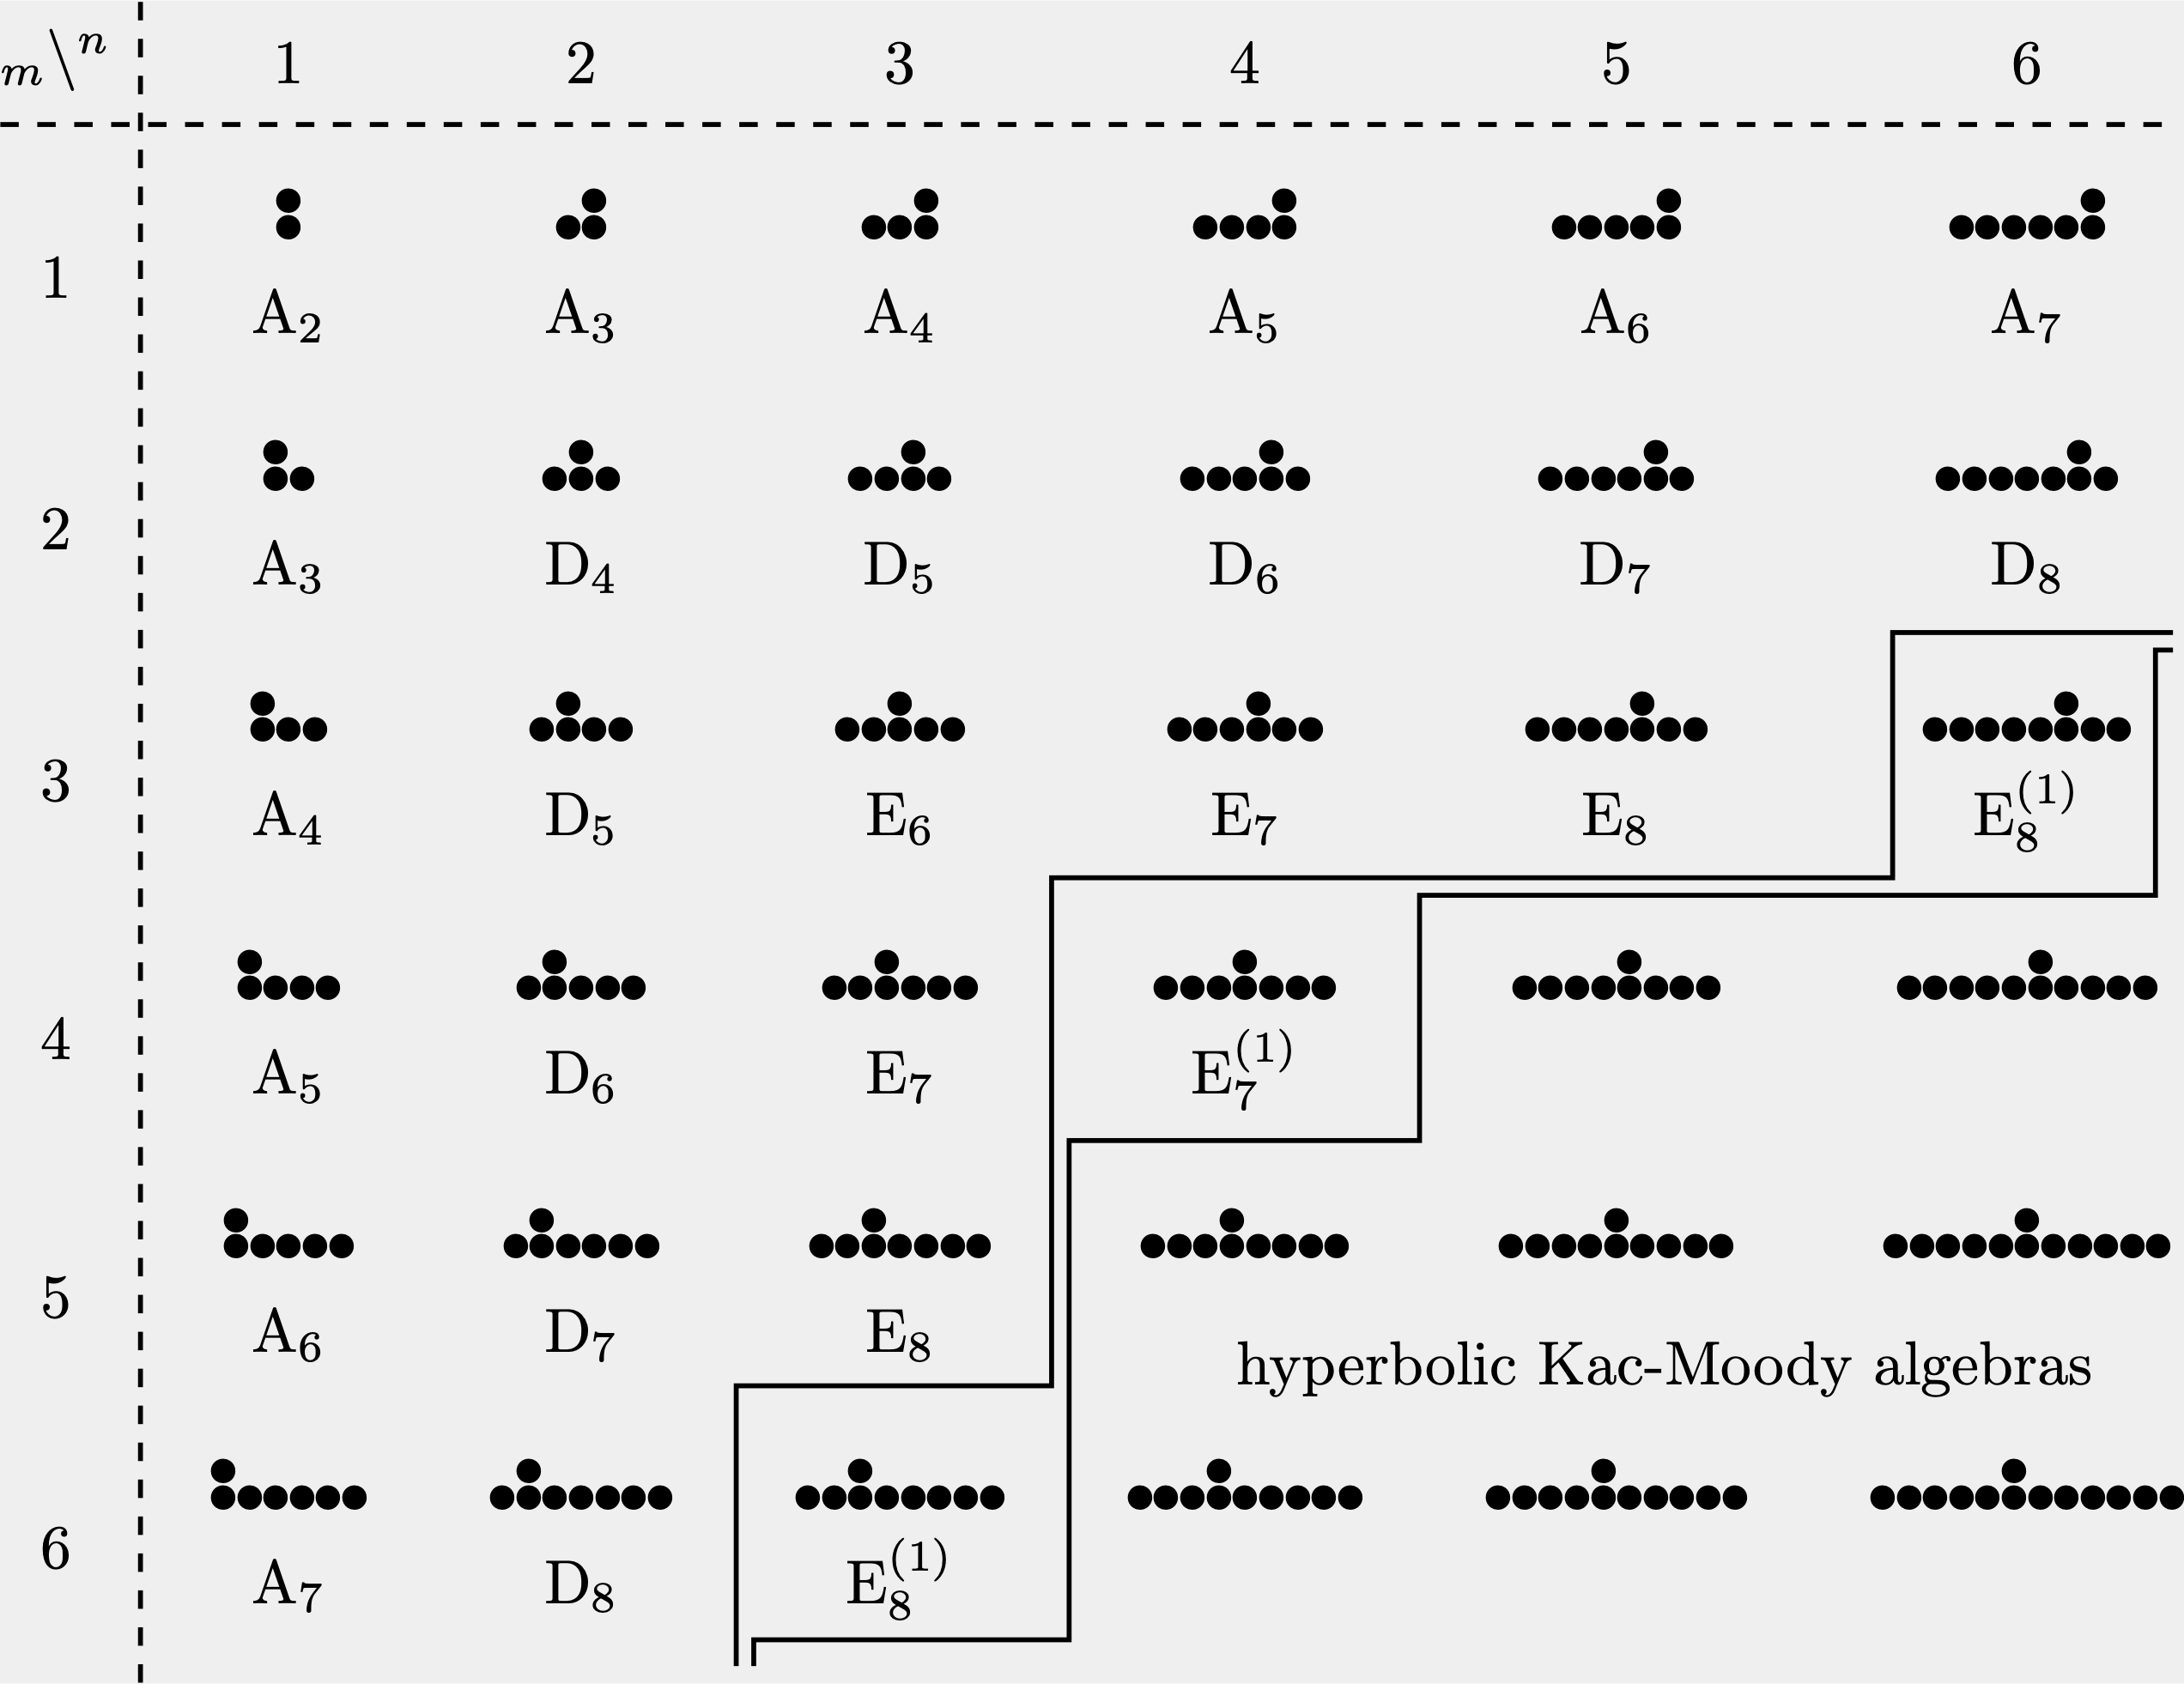
\includegraphics[max width=0.9\linewidth]{../images/week182table.png}\]
This mysterious way that the same Egyptian fraction problem shows up in
classifying Platonic solids and simply-laced simple Lie algebras is
actually the tip an iceberg sometimes called the ``McKay
correspondence'' --- though important aspects of it go back to the
theory of Kleinian singularities. I talked about the McKay
correspondence in \protect\hyperlink{week65}{``Week 65''}, so that's a
good place to dig deeper, but you should really look at some of the
references in there, and also these two --- both of which explain the
mysterious word ``hosohedron'':

\begin{enumerate}
\def\labelenumi{\arabic{enumi})}
\setcounter{enumi}{2}
\item
  H. S. M. Coxeter, \emph{Generators and relations for discrete groups},
  Springer, Berlin, 1984.
\item
  Joris van Hoboken, \emph{Platonic solids, binary polyhedral groups,
  Kleinian singularities and Lie algebras of type \(A\),\(D\),\(E\)},
  Master's Thesis, University of Amsterdam, 2002, available at
  \texttt{http://home.student.uva.nl/joris.vanhoboken/scriptiejoris.ps}
  or
  \texttt{http://math.ucr.edu/home/baez/joris\_van\_hoboken\_platonic.pdf}
\end{enumerate}

Okay. Now --- back to that conference at the Mathematical Sciences
Research Institute! You can look at transparencies and watch videos of
the talks here:

\begin{enumerate}
\def\labelenumi{\arabic{enumi})}
\setcounter{enumi}{4}
\tightlist
\item
  MSRI streaming video archive, Spring 2002,
  \texttt{http://www.msri.org/publications/video/index04.html}
\end{enumerate}

If you like watching math talks, there's a lot to see here --- not just
this one conference, but all the MSRI conferences! For example, right
after the nonabelian Hodge theory conference there was one on conformal
field theory and supersymmetry, featuring talks by bigshots like Richard
Borcherds, Dan Freed, Igor Frenkel, Victor Kac, and Jean-Bernard Zuber
--- just to name a few. You can see talks by all these folks.

But anyway, let me start by telling you what nonabelian Hodge theory
is\ldots.

Hmm. I guess I should \emph{start} by telling you what \emph{abelian}
Hodge theory is!

In its simplest form, Hodge theory talks about how differential forms on
a smooth manifold get extra interesting structure when the manifold has
extra interesting structure. To warm up, let me remind you about what we
can do when our manifold has \emph{no} extra interesting structure.
Whenever we have a smooth manifold \(M\) there's an ``exterior
derivative'' operator \(d\) going from \(p\)-forms on \(M\) to
\((p+1)\)-forms on M. This is just a generalization of grad, curl, div
and all that. In particular it satisfies \[d^2 = 0,\] so the space of
``closed'' \(p\)-forms: \[\{w \mid dw = 0\}\] contains the space of
``exact'' \(p\)-forms: \[\{w \mid \mbox{$w = du$ for some $u$}\}.\] This
makes it fun to look at the vector space of closed \(p\)-forms modulo
exact \(p\)-forms. This is called the ``\(p\)th de Rham cohomology group
of \(M\)'', or \[H^p(M)\] for short. It only depends on the topology of
\(M\); its size keeps track of the number of \(p\)-dimensional holes in
\(M\). When \(M\) is compact, it agrees with the cohomology computed in
a bunch of other ways that topologists like.

Fine. But now, suppose \(M\) has a Riemannian metric on it! Then we can
write down a version of the Laplacian for differential forms. A function
is a \(0\)-form, so we're just generalizing the Laplacian you already
know and love. Differential forms whose Laplacian is zero are called
``harmonic''. Every harmonic \(p\)-form is closed, but if \(M\) is
compact life is even better: the vector space of harmonic \(p\)-forms is
isomorphic to the \(p\)th de Rham cohomology of \(M\).

This is great: it means the de Rham cohomology, which only depends on
the \emph{topology} of \(M\), can also be thought of as the space of
solutions of a \emph{differential equation} on \(M\)! This gets
topologists and analysts talking to each other, and has all sorts of
marvelous spinoffs and generalizations.

Some people call this stuff ``Hodge theory''. But Hodge theory goes
further when \(M\) has more structure --- most notably, when it's a
Kaehler manifold!

A Kaehler manifold is to the complex plane as a Riemannian manifold is
to the real line. More precisely, it's is a manifold whose tangent
spaces have been made into \emph{complex} vector spaces and equipped
with a \emph{complex} inner product. Of course the real part of the
inner product makes it into a Riemannian manifold. That lets us parallel
transport vectors, so we demand a compatibility condition: parallel
transporting a vector and then multiplying it by \(i\) is the same as
multiplying it by \(i\) and then parallel transporting it! This makes
complex analysis work well on Kaehler manifolds.

Now, if you've taken complex analysis, you may remember how people use
it to find solutions of Laplace's equation\ldots{} like when they're
studying electrostatics, or the flow of fluids with no viscosity or
vorticity --- an idealization that von Neumann mockingly called ``dry
water''. On the complex plane we can talk about ``holomorphic''
functions, which satisfy the Cauchy-Riemann equation: \[
  \frac{df}{d\overline{z}} = 0
  \qquad
  \left(
    \text{note:}\,\,
    \frac{df}{d\overline{z}} = \frac{df}{dx} + i\frac{df}{dy}
  \right)
\] and also the complex conjugates of these, called ``antiholomorphic''
functions, which satisfy \[
  \frac{df}{dz} = 0
  \qquad
  \left(
    \text{note:}\,\,
    \frac{df}{dz} = \frac{df}{dx} - i\frac{df}{dy}
  \right)
\] Both holomorphic and antiholomorphic functions are automatically
harmonic, so we can find solutions of Laplace's equation this way. But
even better, every harmonic function is a linear combination of a
holomorphic and an antiholomorphic one!

All this stuff works much more generally for \(p\)-forms on Kaehler
manifolds. To get going, let's think a bit more about the complex plane.
If we have any \(1\)-form on the complex plane we can write it as a
linear combination of \(dx\) and \(dy\), where \(x\) and \(y\) are the
usual coordinates on the plane. But things get nicer if we work with
\emph{complex-valued} differential forms. Then we can form linear
combinations like \[dz = dx + idy\] and \[d\overline{z} = dx - idy\] and
express any \(1\)-form as a linear combination of \emph{these} in a
unique way. We call these the \((1,0)\) and \((0,1)\) parts of our
\(1\)-form.

This means that if we have a function \(f\), we can take its exterior
derivative and chop it into its \((1,0)\) part and \((0,1)\) part:
\[df = \partial f+\overline{\partial}f.\] These guys are called
``Dolbeault operators''.

Anyway, it turns out that \[\overline{\partial}f = 0\] is just a slick
way of writing Cauchy-Riemann equation, which says that \(f\) is
holomorphic. You should check this for yourself! Similarly,
\[\partial f = 0\] says that \(f\) is antiholomorphic.

Now let me say how all this stuff generalizes to arbitrary Kaehler
manifolds. We can decompose any \(p\)-form on a Kaehler manifold into
its \((i,j)\) parts where \(i+j = p\). For example, a \((1,2)\)-form in
\(4\) dimensions might look something like this in complex coordinates:
\[f dz_1\wedge d\overline{z}_3\wedge d\overline{z}_2 + g dz_2\wedge d\overline{z}_3\wedge d\overline{z}_4.\]
We have \[d = \partial + \overline{\partial}\] where \(\partial\) maps
\((i,j)\)-forms to \((i+1,j)\)-forms, while \(\overline{\partial}\) maps
\((i,j)\)-forms to \((i,j+1)\)-forms. This allows us to take the de Rham
cohomology groups of our manifold \(M\) and write them as a direct sum
of smaller vector spaces, which I'll call \[H^{i,j}(M)\] for short.

So far I don't think I've used anything about the metric on \(M\), so
all this would work whenever \(M\) is a so-called ``complex manifold''.
But if we really have a Kaehler manifold, and it's compact, we can say
more: a \(p\)-form is harmonic if and only if all its \((i,j)\) parts
are. This means \(H^{i,j}(M)\) is isomorphic to the space of harmonic
\((i,j)\)-forms. Alternatively, you can describe \(H^{i,j}(M)\) just in
terms of \(\partial\): you just take the \((i,j)\)-forms in here:
\[\{w \mid \overline{\partial}w = 0\}\] modulo those in here:
\[\{w \mid \mbox{$w=\overline{\partial}u$ for some $u$}\}\] This is
called the ``\((i,j)\)th Dolbeault cohomology group of \(M\)''.

That's Hodge theory in a nutshell. There's even \emph{more} you can do
when \(M\) is a Kaehler manifold, but I'm getting a little tired, so
I'll just let you read about that here:

\begin{enumerate}
\def\labelenumi{\arabic{enumi})}
\setcounter{enumi}{5}
\tightlist
\item
  R. O. Wells, \emph{Differential analysis on complex manifolds},
  Springer, Berlin, 1980.
\end{enumerate}

This is a really \emph{great} book for learning about all sorts of good
geometry stuff, starting with differential forms and working on up
through Hodge theory, pseudodifferential operators, sheaves and so on.

But anyway, I've given you a little taste of Hodge theory. The main
thing to remember is that when your manifold is complex, the cohomology
becomes ``bigraded'': instead of just \[H^p(M)\] you get \[H^{i,j}(M).\]
So now, what's nonabelian Hodge theory?

The basic idea is simple: instead of askng what extra structure the
\emph{homology groups} get when \(M\) is a complex manifold, we ask what
extra structure the \emph{homotopy type} of \(M\) gets when \(M\) is a
complex manifold. The homotopy type includes invariants like the
homotopy groups, but also more. How are these constrained by the fact
that \(M\) is complex?

Unfortunately, to describe the answer --- even a little teeny part of
the answer --- I need to turn up the math level a notch.

For starters we can consider the fundamental group \(\pi_1(M)\). But
this is hard to relate to differential geometry, so we will immediately
water it down by picking an algebraic group \(G\) and looking at
homomorphisms of \(\pi_1(M)\) into \(G\). These are basically the same
thing as flat \(G\)-bundles over \(M\), so it's easier to see how \(M\)
being a complex manifold affects things. We can even be sneaky and study
this for all \(G\) at once by forming a group \(\Pi_1(M)\) called the
``proalgebraic completion'' of \(\pi_1(M)\). This is a proalgebraic
group --- an inverse limit of algebraic groups --- which contains
\(\pi_1(M)\) and has the property that any homomorphism from
\(\pi_1(M)\) into an algebraic group \(G\) extends uniquely to a
proalgebraic group homomorphism from \(\Pi_1(M)\) to \(G\).

It's nice to ask what extra structure \(\Pi_1(M)\) gets when \(M\) is a
complex manifold, because this question has a nice answer.

To get ready for how nice the answer is, first go back to plain old
abelian Hodge theory. Note that making the cohomology of \(M\) bigraded
gives an obvious way for the algebraic group \(\mathbb{C}^\times\), the
nonzero complex numbers, to act on the cohomology. The reason is that
for each integer there's a representation of \(\mathbb{C}^\times\) where
the number \(z\) acts as multiplication by \(z^n\), so gradings are just
another way of talking about \(\mathbb{C}^\times\) actions. Since the
cohomology of \(M\) is automatically graded, putting \emph{another}
grading on it amounts to letting \(\mathbb{C}^\times\) act on it.

So in plain old Hodge theory, the answer to ``What extra structure does
the cohomology of \(M\) get when \(M\) is complex?'' is:

\begin{quote}
``It gets an action of \(\mathbb{C}^\times\)!''
\end{quote}

And it turns out that in nonabelian Hodge theory, the answer to ``What
extra structure does \(\Pi_1(M)\) get when \(M\) is complex?'' is:

\begin{quote}
``It gets an action of \(\mathbb{C}^\times\)!''
\end{quote}

This is incredibly cool, but the story goes a lot further. The
fundamental group is just the beginning; you can do something similar
for the higher homotopy groups --- but it's a lot more subtle. In fact,
you can do something similar directly to the homotopy type of \(M\)!
When \(M\) is a compact complex manifold, there's a homotopy type called
the ``schematization of \(M\)'' whose fundamental group is \(\Pi_1(M)\)
--- and there's an action of \(\mathbb{C}^\times\) on this homotopy
type!

By the way, when \(M\) is a compact Kaehler manifold the action of
\(\mathbb{C}^\times\) on its cohomology extends to a natural action of
\(\mathrm{SL}(2,\mathbb{C})\), as explained in Wells' book. I wonder if
\(\mathrm{SL}(2,\mathbb{C})\) acts on the schematization of \(M\)?

I learned about most of this fancy stuff from an incredibly lucid talk
by Bertrand Toen. Unfortunately there seems to be no video of his talk,
since he gave it down the hill at U. C. Berkeley instead of at the MSRI
--- and the handwritten notes at the MSRI website are rather illegible.
So you want to learn more about this, you should probably start with
this quick summary of abelian Hodge theory:

\begin{enumerate}
\def\labelenumi{\arabic{enumi})}
\setcounter{enumi}{6}
\tightlist
\item
  Tony Pantev, ``Review of abelian Hodge theory'',
  \texttt{http://www.msri.org/publications/ln/msri/2002/introstacks/pantev/1/index.html}
\end{enumerate}

and then take the deep plunge into this paper:

\begin{enumerate}
\def\labelenumi{\arabic{enumi})}
\setcounter{enumi}{7}
\tightlist
\item
  Ludmil Katzarkov, Tony Pantev and Bertrand Toen, ``Schematic homotopy
  types and non-abelian Hodge theory I: The Hodge decomposition'',
  available at
  \href{https://arxiv.org/abs/math.AG/0107129}{\texttt{math.AG/0107129}}.
\end{enumerate}

There are a lot of model categories and \(n\)-categories lurking in the
background of this subject, as well as ideas that originated in physics,
like ``Higgs bundles''. For the brave reader I recommend these papers:

\begin{enumerate}
\def\labelenumi{\arabic{enumi})}
\setcounter{enumi}{8}
\tightlist
\item
  Bertrand Toen, ``Toward a Galoisian interpretation of homotopy
  theory'', available as
  \href{https://arxiv.org/abs/math.AT/0007157}{\texttt{math.AT/0007157}}.
\end{enumerate}

This answers the question: ``the fundamental group is to covering spaces
as the whole homotopy type is to\ldots{} what?'' The fact that it's in
French probably makes it easier to understand.

\begin{enumerate}
\def\labelenumi{\arabic{enumi})}
\setcounter{enumi}{9}
\tightlist
\item
  Bertrand Toen and Gabriele Vezzosi, ``Algebraic geometry over model
  categories (a general approach to derived algebraic geometry)'',
  available as
  \href{https://arxiv.org/abs/math.AG/0110109}{\texttt{math.AG/0110109}}.
\end{enumerate}

This is only for badass mathematicians who find algebraic geometry and
homotopy theory insufficiently mindblowing when taken separately. Ever
wondered what an affine scheme would be like if you replaced the ground
field by an \(E_\infty\) ring spectrum? Then this is for you.

(I thank David Eppstein for pointing out the work of Alan Swett.)

\begin{center}\rule{0.5\linewidth}{0.5pt}\end{center}

\begin{quote}
\emph{Geometry may sometimes appear to take the lead over analysis, but
in fact precedes it only as a servant goes before his master to clear
the path and light him on his way.}

--- James Sylvester
\end{quote}



\hypertarget{week183}{%
\section{July 30, 2002}\label{week183}}

I'm now in England, visiting the category theorists in Cambridge. Before
coming here I went to a wonderful conference in honor of Graeme Segal's
60th birthday. Most of the talks there described the marvelous different
ways in which ideas from string theory are spreading throughout
mathematics. I should really tell you about this stuff\ldots{} it's very
cool\ldots{} but right now I'm in the mood for talking about something
simpler: some ways in which ideas from \emph{quantum theory} are
spreading throughout mathematics.

Quantum theory is digging its way ever deeper into the mathematical
psyche: for every branch of math, people seem to be developing a
corresponding quantized version, from ``quantum groups'' to ``quantum
cohomology''. Now there is even a textbook on ``quantum calculus'',
suitable for undergraduates:

\begin{enumerate}
\def\labelenumi{\arabic{enumi})}
\tightlist
\item
  Victor Kac and Pokman Cheung, \emph{Quantum Calculus}, Springer,
  Berlin, 2002.
\end{enumerate}

Indeed, we'll soon see that quantum calculus is based on an even simpler
subject that deserves to be called ``quantum arithmetic''!

This book talks about two modified versions of calculus: the
``\(h\)-calculus'' and the ``\(q\)-calculus''. The letter \(h\) stands
for Planck's constant, while the letter \(q\) stands for quantum. They
are adjustable parameters related by the formula \[q = \exp(ih).\] In
particular, these modified versions of calculus reduce to Sir Isaac
Newton's good old ``classical calculus'' in the limit where \[h \to 0\]
or alternatively, \[q \to 1.\]

One eerie thing about these modified versions of calculus is that people
discovered them before quantum mechanics --- and they even used the
letters ``\(h\)'' and ``\(q\)'' in their formulas! In particular, the
use of the letter ``\(q\)'' seems to go back all the way to Gauss, who
wrote about a \(q\)-analogue of the binomial formula and other things.

So what's the idea? Like many great ideas, it's pathetically simple. To
get the \(h\)-calculus, you just leave out the limit in the definition
of the derivative, using this instead: \[\frac{f(x+h)-f(x)}{h}\] In the
limit as \(h \to 0\), this reduces to the usual derivative.

There is a lot to say about this, but deeper and more mysterious
mathematics arises from the \(q\)-calculus, where we use the
``\(q\)-derivative'': \[\frac{f(qx)-f(x)}{qx-x}\] This reduces to the
usual derivative as \(q \to 1\). Note that the \(h\)-derivative says how
\(f(x)\) changes when you \emph{add} something to \(x\), while the
\(q\)-calculus says how it changes when you \emph{multiply} \(x\) by
something.

Some choices of \(q\) are more interesting than others. If \(q\) is a
complex number with \(|q| = 1\), we can take the \(q\)-derivative of a
function that's defined only on the unit circle in the complex plane!
Multiplying by a unit complex number rotates the unit circle a bit, just
as adding a real number translates the real line. If you think about
this for a while you'll see the relationship between the \(h\)-calculus
and the \(q\)-calculus, and how it's especially nice when we set
\(q = \exp(ih)\).

Alternatively, if \(q\) is an integer, we can take the \(q\)-derivative
of a function that's defined only on the integers! This is especially
cool when \(q\) is a prime or a power of a prime; then there are nice
connections to algebra.

Pretty much anything you can do with calculus, you can do with the
\(q\)-calculus. There are \(q\)-integrals, \(q\)-trigonometric
functions, \(q\)-exponentials, and so on. If you try books like this:

\begin{enumerate}
\def\labelenumi{\arabic{enumi})}
\setcounter{enumi}{1}
\tightlist
\item
  George E. Andrews, Richard Askey, Ranjan Roy, \emph{Special
  Functions}, Cambridge U. Press, Cambridge, 1999.
\end{enumerate}

you'll see there are even \(q\)-analogues of all the special functions
you know and love --- Bessel functions, hypergeometric functions and so
on. And like I said, the really weird thing is that people invented them
\emph{before} their relation to quantum mechanics was understood.

I can't possibly explain all this stuff here, but a good way to get
started is to look at the \(q\)-analogue of Taylor's formula. In
ordinary calculus this formula says how to reconstruct any sufficiently
nice function from its derivatives at zero:
\[f(x) = f(0) + f'(0) x + f''(0)\frac{x^2}{2!} + \ldots\] In
\(q\)-calculus we can write down the \emph{exact} same formula using
\(q\)-derivatives and \(q\)-factorials! The \(n\)th \(q\)-derivative of
a function is defined in the obvious way, by taking the \(q\)-derivative
over and over. Let's do this to the function \(x^n\). If we take its
\(q\)-derivative \emph{once} we get:
\[\frac{(qx)^n-x^n}{qx-x} = \frac{q^n-1}{q-1}x^{n-1}\] We can make this
look almost like the usual derivative of \(x^n\) if we define the
``\(q\)-integer'' \([n]\) by
\[[n] = \frac{q^n-1}{q-1} = 1+q+q^2+\ldots+q^{n-1}\] Then the
\(q\)-derivative of \(x^n\) is just \[[n] x^{n-1}\] This implies that
the \(n\)th \(q\)-derivative of \(x^n\) is the ``\(q\)-factorial''
\[[n]! = [1] [2] \ldots [n] \] This in turn means that the usual Taylor
formula still works if we replace derivatives by \(q\)-derivatives and
factorials by \(q\)-factorials.

Now, starting with \(q\)-factorials we can define \(q\)-binomial
coefficients: \[\frac{[n]!}{[m]![n-m]!}\] and then cook up a
\(q\)-Pascal's triangle, prove a \(q\)-binomial theorem, and so on. It's
not just a matter of recapitulating ordinary calculus, either:
eventually we run into lots of cool identities that have no classical
analogues, like the ``Jacobi triple product formula'':
\[\sum_{n\in\mathbb{Z}} q^{\frac{n(n+1)}{2}}x^n = \prod_{i\in\mathbb{N}^{\geqslant0}} (1+xq^i)(1+x^{-1}q^{i-1})(1-q^i)\]
Now, personally I'm not a big fan of identities just for the sake of
identities. However, I like taking identities and trying to find their
``secret inner meaning'' --- mainly by seeing how they come from
isomorphisms between interesting mathematical structures. The mysterious
identities of \(q\)-mathematics provide an ample playground for this
game, especially since they're all related in intricate ways.

If you ever get stuck on a desert island you can have lots of fun
reinventing quantum calculus, and if you \emph{don't}, you can read Kac
and Cheung's book. So either way, there's no point in me describing its
contents further; instead, I want to say more about how
\(q\)-mathematics is related to physics.

For starters, let's see how the canonical commutation relations change
when we use a \(q\)-derivative to define the momentum operator, instead
of an ordinary derivative. Remember what Schroedinger said: a particle
on a line is described by a ``wavefunction'', which is a complex
function on the line, say \(\psi\). The position operator \(Q\)
multiplies a wavefunction by \(x\): \[(Q \psi)(x) = x \psi(x)\] while
the momentum operator \(P\) basically takes their derivative:
\[(P \psi)(x) = -i \psi'(x)\] The canonical commutation relations say
that \[PQ - QP = -i.\] Now, how does this change if we define the
momentum operator using the \(q\)-derivative instead? I could do this
calculation for you, but you'll be a much better person if you do it
yourself --- it's incredibly easy, so \emph{please} do it. The answer is
\[PQ-qQP = -i.\] In other words, we must replace the commutator
\(PQ - QP\) by a ``\(q\)-commutator''. This is the tip of a big iceberg:
the whole theory of Lie algebras has a ``\(q\)-deformed'' version where
\(q\)-commutators of various sorts take the place of commutators --- and
just as Lie algebras go along with Lie groups, these \(q\)-deformed Lie
algebras go along with ``quantum groups''.

Now let's check to see if you're paying attention. The alert reader
should have already noticed an incredible glaring contradiction in what
I've said! I put it there on purpose, to make an important point.

No? It's simple. I said that making \(q\) different from \(1\) is like
making Planck's constant different from \(0\) --- going from classical
to quantum. People working on quantum groups often say this. But look
what we just did! We took the canonical commutation relations, which are
\emph{already} quantum-mechanical, and modified \emph{them} by making
\(q\) different from 1. This is blatantly obvious if we put Planck's
constant where it belongs in the above formulas, instead of hiding it by
setting it equal to \(1\). The momentum operator is really
\[(P \psi)(x) = -i \hbar \psi'(x)\] so the canonical commutation
relations are \[PQ - QP = -i \hbar\] and when we use a \(q\)-derivative
in the momentum operator they become \[PQ - qQP = -i \hbar.\] So there
really are \emph{two} adjustable parameters floating around: Planck's
constant and this mysterious new ``\(q\)''!

In fact, I've been complaining about this for years: it's only in
certain special contexts that you can think of the ``\(q\)'' or
``\(h\)'' in quantum calculus as related to Planck's constant; here's
one in which they're obviously distinct. So what's the physical meaning
of \(q\)-deformation?

One person to take a stab at this is Shahn Majid:

\begin{enumerate}
\def\labelenumi{\arabic{enumi})}
\setcounter{enumi}{2}
\tightlist
\item
  Shahn Majid, \emph{Foundations of Quantum Group Theory}, Cambridge U.
  Press, Cambridge, 2000.
\end{enumerate}

In this book he says \(q\) is related to Newton's gravitational
constant. This would be cool, because then you could take your theory of
quantum gravity, full of formulas like \[PQ - qQP = -i \hbar,\] and make
the quantum effects small by letting \(\hbar \to 0\), or make the
gravitational effects go away by setting \(q \to 1\). The problem is,
I've never seen a theory of quantum gravity like this! Neither loop
quantum gravity nor string theory work this way.

In fact, both loop quantum gravity people and string theorists agree on
how to quantize gravity without matter in 3 spacetime dimensions. This
is about the \emph{only} thing they agree on. Quantum gravity in 3
dimensions is full of \(q\)-mathematics, and in this theory \(q\) is the
exponential of something involving the \emph{cosmological constant}.
When \(q = 1\) you get the quantum theory of flat 3d spacetime, since
then Einstein's equations say that spacetime is flat --- this is a
peculiarity of 3 dimensions. But when \(q\) is different from \(1\), you
get the quantum theory of a spacetime having constant curvature: a
nonzero cosmological constant means the vacuum has energy density, which
curves spacetime!

For some interesting new insights into this, see:

\begin{enumerate}
\def\labelenumi{\arabic{enumi})}
\setcounter{enumi}{3}
\tightlist
\item
  John Barrett, ``Geometrical measurements in three-dimensional quantum
  gravity'', available as
  \href{https://arxiv.org/abs/gr-qc/0203018}{\texttt{gr-qc/0203018}}.
\end{enumerate}

When we make the cosmological constant nonzero in 3d quantum gravity we
must replace the group \(\mathrm{SU}(2)\) by the quantum group
\(\mathrm{SU}_q(2)\). Based on this, one can argue that quantum groups
are misnamed --- they should really be called ``cosmological groups''.
Another way to put it is this: ordinary groups are already perfectly
sufficient for most of quantum theory; quantum groups show up only in
certain special contexts.

This goes to show that the deep inner meaning of the ``\(q\)'' in
quantum groups is still up for debate. Mathematically it has a lot to do
with replacing groups by non-cocommutative Hopf algebras, whose
representations form a braided rather than symmetric monoidal category.
Here Majid and I agree completely: Planck's constant is about deviations
from commutativity while this ``\(q\)'' stuff is about deviations from
co-commutativity, or the failure of braidings to be symmetric. Still, I
think one should try to understand this more deeply. The amazing things
that happen when \(q\) is a power of a prime number have got to be an
important clue! I'll talk about this more next week.

\begin{center}\rule{0.5\linewidth}{0.5pt}\end{center}

\textbf{Addendum:} Toby Bartels brought up an important point in a reply
on the newsgroup \texttt{sci.physics.research}:

\begin{quote}
John Baez wrote in small part:
\end{quote}

\begin{quote}
\begin{quote}
In fact, I've been complaining about this for years: it's only in
certain special contexts that you can think of the ``\(q\)'' or
``\(h\)'' in quantum calculus as related to Planck's constant; here's
one in which they're obviously distinct. So what's the physical meaning
of \(q\)-deformation?
\end{quote}
\end{quote}

\begin{quote}
If \(q = \exp h\), then \(h\) couldn't possibly be Planck's constant,
because Planck's constant is not dimensionless. (Or when you make it
dimensionless, you generally fix its value, and then it makes no sense
to speak of varying \(q\).) To get a dimensionless constant for \(h\),
use (\(\hbar G \Lambda/c^3\)), where \(\hbar\) = Planck's constant,
\(G\) = Newton's constant, \(\Lambda\) = cosmological constant, and
\(c\) = speed of light.
\end{quote}

\begin{quote}
If you're coming from the POV where you only had 3 of these before, with
the 4th equal to \(0\) (or infinite in the case of \(c\)), then you're
going to view changing from \(q = 1\) to some other \(q\) as varying the
value of the 4th constant. Thus John (a quantum gravity theorist that
often sets \(\hbar\), \(G\), and \(c\) to fixed values) thinks that it's
\(\Lambda\), while Majid (who studied quantum field theory, which fixes
\(\hbar\) and \(c\) and thinks of \(\Lambda\) as a fixed QFT
effect){[}*{]} thinks that it's \(G\). But it is the dimensionless ratio
that matters to everybody.
\end{quote}

\begin{quote}
{[}*{]}I'm being presumptuous here.
\end{quote}

\begin{quote}
-- Toby Bartels
\end{quote}

I replied:

\begin{quote}
Toby Bartels wrote:

\begin{quote}
John Baez wrote in small part:
\end{quote}

\begin{quote}
\begin{quote}
In fact, I've been complaining about this for years: it's only in
certain special contexts that you can think of the ``\(q\)'' or
``\(h\)'' in quantum calculus as related to Planck's constant; here's
one in which they're obviously distinct. So what's the physical meaning
of \(q\)-deformation?
\end{quote}
\end{quote}

\begin{quote}
If \(q = \exp h\), then \(h\) couldn't possibly be Planck's constant,
because Planck's constant is not dimensionless. (Or when you make it
dimensionless, you generally fix its value, and then it makes no sense
to speak of varying \(q\).)
\end{quote}

It might make sense to treat Planck's constant as dimensionless and
still talk of varying its value.

However, you're certainly right about this: in applications of
\(q\)-mathematics to quantum gravity, we make Planck's constant
dimensionless by combining it with Newton's gravitational constant, the
speed of light, and the cosmological constant in this way:

\begin{quote}
To get a dimensionless constant for \(h\), use
(\(\hbar G \Lambda/c^3\)), where \(\hbar\) = Planck's constant, \(G\) =
Newton's constant, \(\Lambda\) = cosmological constant, and \(c\) =
speed of light.
\end{quote}

\ldots{} or something like that. I think the formula depends on the
dimension of spacetime, and so far it's in \((2+1)\)d spacetime that all
the really solid applications of \(q\)-mathematics to quantum gravity
arise. But the basic idea is robust, and it doesn't depend on the
dimension of spacetime:

We get a dimensionless constant by measuring the density of the vacuum
in Planck masses per Planck volume!

In other words: using \(\hbar\) \(G\) and \(c\) we can construct units
of length, time, mass and so on --- and then we can talk about the
energy density of the vacuum, measured in those units, and get something
dimensionless.

This explains why \(q\)-mathematics only shows up when we do quantum
gravity with a nonzero cosmological constant (or perhaps matter).

\begin{quote}
If you're coming from the POV where you only had 3 of these before, with
the 4th equal to 0 (or infinite in the case of \(c\)), then you're going
to view changing from \(q = 1\) to some other \(q\) as varying the value
of the 4th constant. Thus John (a quantum gravity theorist that often
sets \(\hbar\), \(G\), and \(c\) to fixed values) thinks that it's
\(\Lambda\) {[}\ldots{]}
\end{quote}

Right. Actually, the real reason I like to claim it's \(\Lambda\) is
that this is the most surprising of the four alternatives.
\end{quote}

\begin{center}\rule{0.5\linewidth}{0.5pt}\end{center}

\begin{quote}
\emph{When we try to pick out anything by itself, we find it hitched to
everything else in the Universe.}

--- John Muir
\end{quote}



\hypertarget{week184}{%
\section{August 4, 2002}\label{week184}}

To really know a subject you've got to learn a bit of its history. If
that subject is topology, you've got to read this:

\begin{enumerate}
\def\labelenumi{\arabic{enumi})}
\tightlist
\item
  I. M. James, editor, \emph{History of Topology}, Elsevier, New York,
  1999.
\end{enumerate}

From a blow-by-blow account of the heroic papers of Poincare to a
detailed account by Peter May of the prehistory of stable homotopy
theory\ldots{} it's all very fascinating. You'll probably want to study
some more of the subject by the time you're done!

In order to satisfy that craving, I want to tell you how to compute some
homology groups. But we'll do it a strange way: using
``\(q\)-mathematics''. I began talking about \(q\)-mathematics last
week, but now I want to dig deeper.

At first, it looks like there are two really \emph{different} places
where this \(q\)-stuff shows up. One is when you do mathematics with
\(q\)-deformed quantum groups replacing the Lie groups you know and love
--- this is important in string theory, knot theory, and loop quantum
gravity. In this case it's best if \(q\) is a unit complex number,
especially an nth root of unity:
\[q = \exp\left(\frac{2\pi i}{n}\right)\] You'll notice that in string
theory, knot theory and loop quantum gravity, \emph{loops} play a big
role. This is no coincidence; in a way, quantum groups are just a
technical device for studying ``loop groups'', which are groups
consisting of functions from a circle to some specified Lie group.

See, in quantum physics problems with a loop group as the symmetry
group, these symmetries tend to hold only \emph{up to a phase}. The
precise way these phases work depends on the parameter \(q\).
Mathematically, this means that instead the loop group itself, the
symmetries are really described by a slightly larger group that keeps
track of these phases, called a ``central extension'' of the loop group.
This has led people to spend huge amounts of energy studying
representations of central extensions of loop groups --- which turn out
to be much more economically understood, in a rather subtle way, as
representations of quantum groups. In all this work the parameter \(q\)
plays a major role.

For more on this try these books:

\begin{enumerate}
\def\labelenumi{\arabic{enumi})}
\setcounter{enumi}{1}
\item
  Andrew Pressley and Graeme Segal, \emph{Loop Groups}, Oxford U. Press,
  Oxford, 1986.
\item
  Vyjayanathi Chari and Andrew Pressley, \emph{A Guide to Quantum
  Groups}, Cambridge U. Press, Cambridge, 1994.
\item
  Jürgen Fuchs, \emph{Affine Lie Algebras and Quantum Groups}, Cambridge
  U. Press, Cambridge, 1992.
\end{enumerate}

Taken together, they provide a pretty good view of what I'm talking
about. In case you're wondering, an ``affine Lie algebra'' is the Lie
algebra of a central extension of a loop group.

Mathematical physicists know all about this sort of \(q\)-stuff. But
\(q\)-stuff also shows up when we do mathematics with finite fields.
Here I don't mean ``field'' in the physics sense --- I mean an algebraic
gadget where you can add, subtract, multiply and divide! Physicists are
happiest when their field is the real or complex numbers. But
mathematicians also like fields with finitely many elements. If \(q\) is
a power of a prime number, there is a unique field with \(q\) elements,
called \(\mathbb{F}_q\). Even better, these are \emph{all} the finite
fields. If \(q\) is itself prime, \(\mathbb{F}_q\) is just the integers
\(\mod q\). We can get the other finite fields using a trick very much
like how we get the complex numbers from the reals by throwing in the
square root of minus one.

Don't be scared: this is already \emph{more} than what you'll need to
know about finite fields to understand what I'm going to say!

And here's what I'm going to say: lots of formulas for counting
structures on finite sets have \(q\)-versions that tell you how to count
structures on projective spaces over \(\mathbb{F}_q\). Remember, a
``projective space'' is just the space of all line through the origin in
a vector space. The basic idea is this mystical analogy:

\begin{longtable}[]{@{}ll@{}}
\toprule
\endhead
\(q=1\) & finite sets\tabularnewline
\(q=p^n\) for \(p\) prime & projective spaces over
\(\mathbb{F}_q\)\tabularnewline
\bottomrule
\end{longtable}

This analogy is so powerful that it really pays to think of finite sets
as projective spaces over \(\mathbb{F}_1\), the ``field with one
element'' --- even though there is no such field!

Let's start with some examples. How many points does an \(n\)-element
set have? Answer: the integer \[n.\] Next: how many lines through the
origin does an \(n\)-dimensional vector space over \(\mathbb{F}_q\)
have? Of course, these lines are points in the corresponding projective
space. Answer: the \(q\)-integer
\[[n] = \frac{q^n-1}{q-1} = 1+q+q^2+\ldots+q^{n-1}.\] Remember from last
week that the basic idea behind ``\(q\)-arithmetic'' was to replace
integers by these \(q\)-integers. To see why this answer is right, first
note that we determine a line through the origin by picking any nonzero
vector. There are \(q^n - 1\) of these. However, two vectors determine
the same line if one is a nonzero multiple of the other, and there are
\(q - 1\) nonzero elements of \(\mathbb{F}_q\). So, the actual number of
lines through the origin is \[\frac{q^n-1}{q-1} = [n].\]

Here's another example. How many ways are there to order a set with
\(n\) elements? Answer: \[n!=1\cdot2\cdot\ldots\cdot n.\] Next: how many
maximal flags are there in an \(n\)-dimensional vector space over
\(\mathbb{F}_q\)? Answer: the \(q\)-factorial
\[[n]! = [1][2]\ldots[n].\] Remember, a maximal flag is a line through
the origin contained in a plane through the origin contained in \ldots{}
and so on, up to the top dimension. As we've seen, there are \([n]\)
ways to choose a line \(L\) like this in our vector space \(V\). The
next step is to choose a plane containing \(L\). This is the same as
choosing a line in the quotient space \(V/L\), which has one dimension
less, so there are \([n-1]\) ways to do this. And so on, giving us
\([n]!\) maximal flags.

Here's yet another example. How many \(m\)-element subsets does an
\(n\)-element set have? Answer: the binomial coefficient
\[\frac{n!}{m!(n-m)!}\] Next: how many \(m\)-dimensional subspaces are
there of an \(n\)-dimensional space over \(\mathbb{F}_q\)? Answer: the
\(q\)-binomial coefficient \[\frac{[n]!}{[m]![n-m]!}\] I'll leave this
one as an exercise.

It goes on and on like this: all sorts of structures that can be defined
for finite sets have analogues for the projective geometry of finite
fields, and when we count these, the former tend to give us ``ordinary
mathematics'', while the latter give us ``\(q\)-mathematics'', which
reduces to ordinary mathematics at \(q = 1\).

Clearly this pattern is trying to tell us something; the question is
what. As always, it pays to focus on the simplest case, since that's
where everything starts. I said that the number of lines through the
origin in an \(n\)-dimensional vector space over the field with \(q\)
elements is \[[n] = \frac{q^n-1}{q-1} = 1+q+q^2+\ldots+q^{n-1}.\] But
now let's think about why the \emph{second} equation here is true!

Of course this is just the formula for summing a geometric series, but
we can also categorify this formula. In other words: we can think of
\([n]\) not as the mere \emph{number} of lines through the origin in an
\(n\)-dimensional vector space over \(\mathbb{F}_q\), but as the actual
\emph{set} of such lines. To prove the second equation, we should thus
find a nice way to write this set as \(1\) special line, together with
\(q\) more lines, and then \(q^2\) more, and so on.

To do this, pick a maximal flag: a 1d subspace contained in a 2d
subspace contained in a 3d subspace\ldots{} and so on. There is one line
through the origin contained in our 1d subspace --- namely the subspace
itself. There are \(q\) lines through the origin contained in the 2d
subspace but not in the 1d subspace. There are \(q^2\) lines in the 3d
subspace but not the 2d subspace. And so on. \emph{Voila!}

Combinatorists call this a ``bijective proof'': a proof that two numbers
are equal which actually establishes a bijection between the finite sets
they count. It's an example of ``categorification'' because we've taken
an equation and found the isomorphism that explains it --- taking us
from math in the \emph{set} of natural numbers to math in the
\emph{category} of finite sets.

The cool part is, this proof works for \emph{all} fields, not just
finite ones. For example, over the real numbers we can use it to take
the projective space \(\mathbb{RP}^{n-1}\) and chop it into pieces like
this:
\[\mathbb{RP}^{n-1} = \mathbb{R}^0 + \mathbb{R}^1 + \ldots + \mathbb{R}^{n-1}\]
Topologically speaking, we've just decomposed \(\mathbb{RP}^{n-1}\) as a
union of open balls, or ``cells''. This makes it easy to calculate its
Euler characteristic. Even-dimensional cells contribute \(1\) to the
Euler characteristic, while odd-dimensional cells contribute \(-1\), so
we get
\[|\mathbb{RP}^{n-1}| = (-1)^0 + (-1)^1 + \ldots + (-1)^{n-1} = \frac{(-1)^n-1}{(-1)-1}\]
or in other words, \(0\) if \(n\) is even and \(1\) if \(n\) is odd.
Here I'm using \(|X|\) to stand for the Euler characteristic of \(X\).

You'll notice that the Euler characteristic is working here exactly like
the cardinality did in the finite field case. That's no coincidence! The
Euler characteristic and its evil twin the ``homotopy cardinality'' are
both generalizations of cardinality, as I explained in
\protect\hyperlink{week147}{``Week 147''}. If we use Schanuel's improved
version of the Euler characteristic, which lets us chop up a space \(X\)
and calculate \(|X|\) by summing the Euler characteristics of the
pieces, we have \(|\mathbb{R}| = -1\), so
\[|\mathbb{RP}^{n-1}| = |\mathbb{R}^0+\mathbb{R}^1+\ldots+\mathbb{R}^{n-1}| = |\mathbb{R}|^0+|\mathbb{R}|^1+\ldots+|\mathbb{R}|^{n-1} = [n]\]
where \([n]\) is the \(q\)-integer where \(q = |\mathbb{R}| = -1\). So
if you want to shock your friends, you can tell them that the real
numbers are the field with \(-1\) elements!

What about the complex numbers? Well, as spaces we have
\[\mathbb{C} = \mathbb{R}^2\] so we get
\[|\mathbb{C}| = |\mathbb{R}|^2 = 1.\] This implies that the Euler
characteristic of \(\mathbb{CP}^{n-1}\) is \([n]\), where now
\(q = |\mathbb{C}| = 1\). In other words, it's just \(n\).

Now that we've gotten this wonderful new insight we can test it on
fancier examples, like flag manifolds. I already showed you that the
number of maximal flags in an \(n\)-dimensional vector space over
\(\mathbb{F}_q\) is the \(q\)-factorial \[[n]!\] And if you look back,
you'll see I gave a bijective proof. This means that if we work over the
real or complex numbers, the same proof gives a cell decomposition of
the \emph{manifold} of maximal flags in \(\mathbb{R}^n\) or
\(\mathbb{C}^n\) --- the ``flag manifold'', for short. So we can just
calculate some \(q\)-factorials: \[
  \begin{aligned}
    [1]! &= 1
  \\\,[2]! &= 1 + q
  \\\,[3]! &= 1 + 2q + 2q^2 + q^3 
  \\\,[4]! &= 1 + 3q + 5q^2 + 6q^3 + 5q^4 + 3q^5 + q^6
  \end{aligned}
\] and read off all sorts of fun stuff. For example, the flag manifold
of \(\mathbb{R}^4\) has a cell decomposition like
\[\mathbb{R}^0 + 3\mathbb{R} + 5\mathbb{R}^2 + 6\mathbb{R}^3 + 5\mathbb{R}^4 + 3\mathbb{R}^5 + \mathbb{R}^6\]
meaning that there's 1 zero-cell, 3 one-cells, 5 two-cells and so on.
Similarly, the flag manifold of \(\mathbb{C}^4\) has a cell
decomposition like
\[\mathbb{C}^0 + 3\mathbb{C} + 5\mathbb{C}^2 + 6\mathbb{C}^3 + 5\mathbb{C}^4 + 3\mathbb{C}^5 + \mathbb{C}^6\]
meaning that there's 1 zero-cell, 3 two-cells, 5 four-cells and so on.
(Their dimensions are twice as big now, since \(\mathbb{C}\) has
dimension 2.)

In particular, the Euler characteristic of the flag manifold in \(n\)
dimensions is just \([n]!\), where we set \(q = -1\) in the real case
and \(q = 1\) in the complex case. But in the complex case we can say
more!

Whenever you build a space from cells, you can compute its homology from
a chain complex with one generator for each cell and a differential
saying how the cells of dimension \(n\) are glued to the cells of
dimension \(n-1\). But since the complex flag manifold is built from
only even-dimensional cells, the differential is zero in this case. This
means you can read off its \(n\)th homology group by just counting the
number of \(n\)-cells! The homology group is just \(\mathbb{Z}^k\),
where \(k\) is this number.

So for example, if some nasty guy demands that you calculate the 10th
homology of the complex flag manifold in 4 dimensions, you just tell him
``I know it's a free abelian group\ldots{}'' and calculate \[
  \begin{aligned}
    [4]! &= 1 (1 + q) (1 + q + q^2) (1 + q + q^2 + q^3) 
  \\&= 1 + 3q + 5q^2 + 6q^3 + 5q^4 + 3q^5 + q^6
  \end{aligned}
\] You know the \(q^5\) term gives you the \(10\)-cells in this flag
manifold, since the complex numbers have dimension 2. You see the
coefficient of this term is \(3\), so you say ``\ldots{} and it's
\(\mathbb{Z}^3\).'' He will then think you know algebraic topology, and
go away.

The same sort of trick works for Grassmannians, too. The Grassmannian
\(\mathrm{Gr}(n,k)\) is the set of all \(k\)-dimensional subspaces of an
\(n\)-dimensional vector space. This makes sense over any field. I
already said that over the finite field \(\mathbb{F}_q\), the
cardinality of this Grassmannian is the \(q\)-binomial coefficient
\[|\mathrm{Gr}(n,k)| = \frac{[n]!}{[k]![n-k]!}\] The same formula gives
the Euler characteristic of this Grassmannian over the real numbers if
we set \(q = -1\), and over the complex numbers if we set \(q = 1\). Of
course \(q = 1\) just gives the ordinary binomial coefficients.

So, for example, the Euler characteristic of the manifold of
\(2\)-dimensional subspaces of \(\mathbb{C}^4\) is the same as the
number of ways of choosing \(2\) elements from a \(4\)-element set! A
nice example of the unity of mathematics.

Also, since complex Grassmannians are built from only even-dimensional
cells, we can read off their homology groups just like we did for
complex flag manifolds. Let's work out the homology of
\(\mathrm{Gr}(4,2)\), for example. We start by working out the
\(q\)-binomial coefficient:
\[\frac{[4]!}{[2]![2]!} = \frac{1(1+q)(1+q+q^2)(1+q+q^2+q^3)}{1(1+q)1(1+q)} = 1+q+2q^2+q^3+q^4.\]
It's mildly surprising that this ratio works out to be a polynomial, but
of course we know it must! Reading off the coefficients, we get:

\begin{itemize}
\tightlist
\item
  the \(0\)th homology group is \(\mathbb{Z}\)
\item
  the \(2\)nd homology group is \(\mathbb{Z}\)
\item
  the \(4\)th homology group is \(\mathbb{Z}^2\)
\item
  the \(6\)th homology group is \(\mathbb{Z}\)
\item
  the \(8\)th homology group is \(\mathbb{Z}\)
\end{itemize}

and while we're at it, we've learned this Grassmannian is 8-dimensional
as a \emph{real} manifold --- or \(4\)-dimensional as a complex
manifold. Note how the \(n\)th homology group is the same as the
\((8-n)\)th; this comes from Poincare duality.

On a lighter note: the best way to simplify this sort of expression
\[\frac{1(1+q)(1+q+q^2)(1+q+q^2+q^3)}{1(1+q)1(1+q)}\] is to use base
\(q\). Then it's just
\[\frac{1\times11\times111\times1111}{1\times11\times1\times11} = \frac{111\times1111}{11} = \frac{123321}{11} = 11211\]
where I did the last step using long division. And of course the last
quantity is \[1+q+2q^2+q^3+q^4.\] By the way, the cells we've been
counting are called ``Schubert cells''.

I'll quit here for now, but actually this is just the tip of the
iceberg. I've been talking how \(q\)-factorials are related to
projective geometry, but as readers of
\protect\hyperlink{week178}{``Week 178''},
\protect\hyperlink{week180}{``Week 180''} and
\protect\hyperlink{week181}{``Week 181''} will know, there exists a
generalization of projective geometry for any simple Lie group. In fact,
for \emph{any} simple Lie group \(G\) and \emph{any} parabolic subgroup
\(P\) there is a decomposition of \(G/P\) into Schubert cells, and these
cells are counted by the coefficients of a certain polynomial in \(q\).
Using these you can massively generalize everything I just told you!
I'll explain this stuff in future Weeks.

\begin{center}\rule{0.5\linewidth}{0.5pt}\end{center}

\textbf{Addendum:} Here's my reply to a request for clarification from
my friend Squark:

\begin{quote}
Squark wrote:

\begin{quote}
John Baez wrote:
\end{quote}

\begin{quote}
\begin{quote}
If we use Schanuel's improved version of the Euler characteristic, which
lets us chop up a space \(X\) and calculate \(|X|\) by summing the Euler
characteristics of the pieces, we have \(|\mathbb{R}| = -1\),
\(\mathbb{C} = \mathbb{R}^2\), so we get
\[|\mathbb{C}| = |\mathbb{R}|^2 = 1.\] How does this Schanuel thingie
work? \(\mathbb{R}\) and \(\mathbb{C}\) are both contractible, so it has
to be principally different from the usual Euler characteristic!
\end{quote}
\end{quote}

Right. Schanuel's Euler characteristic is not homotopy invariant like
the usual Euler characteristic, and it's only defined for nice spaces,
like polyhedral sets. However, it has a great property to make up for
these sins: whenever we can chop up a polyhedral set \(A\) into nice
parts \(B\) and \(C\), we have \[|A| = |B| + |C|\] We also have
\[|X\times Y| = |X| \times |Y|,\] and homeomorphic nice spaces have the
same Schanuel Euler characteristic. One can check that for compact
manifolds, the Schanuel Euler characteristic matches the usual one, so
my strange calculations really do give the standard ``right answers''.

Schanuel's Euler characteristic of a point is \(1\): \[|*| = 1\] so the
Schanuel Euler characteristic of the open interval must be \(-1\): we
have \[(0,1) = (0,1/2) + \{1/2\} + (1/2,1)\] so if \[|(0,1)| = x\] we
have \[x = x + 1 + x\] so \(x = -1\).

This means that the Schanuel Euler characteristic of a half-open
interval is zero: \[(0,1] = (0,1) + \{1\}\] so
\[|(0,1]| = |(0,1)| + |\{1\}| = -1+1 = 0.\] The Schanuel Euler
characteristic of a circle is \(0\) as well, since we can chop it into
two (or three, or more) half-open intervals.

The Schanuel Euler characteristic of an open square is \(1\):
\[|(0,1)\times(0,1)| = |(0,1)|\times|(0,1)| = -1\times-1 = 1\] and the
S-E characteristic of a closed square is \(1\times1 = 1\).

Now, just as a consistency check, write the closed square as the union
of an open square and its boundary. The boundary is homeomorphic to a
circle, so we should get \(1 + 0 = 1\). It works!

A good reference on this stuff is:

James Propp, ``Exponentiation and Euler measure'', available at
\texttt{http://www.arXiv.org/abs/math.CO/0204009}.

Here you'll see that what I'm calling Schanuel's Euler characteristic
goes back to work before Schanuel. Also, if you push it far enough, it
gives a fascinating approach to dealing with ``sets with negative
numbers of elements'' --- for example, it gives a kind of combinatorial
interpretation of identities like \[\binom{-2}{3} = -4\] Schanuel was
trying to categorify the integers: that's why he came up with this
stuff.

Also see \protect\hyperlink{week147}{``Week 147''} for more!
\end{quote}

\begin{center}\rule{0.5\linewidth}{0.5pt}\end{center}

\begin{quote}
\emph{We should declare instead candidly that we dwell on mathematics
and affirm its statements for the sake of its intellectual beauty, which
betokens the reality of its conceptions and the truth of its assertions.
For if this passion were extinct, we would cease to understand
mathematics; its conceptions would dissolve and its proofs carry no
conviction.}

--- Michael Polyani
\end{quote}



\hypertarget{week185}{%
\section{August 30, 2002}\label{week185}}

I'd like to continue the story of ``\(q\)-mathematics'' which I was
telling you in \protect\hyperlink{week183}{``Week 183''} and
\protect\hyperlink{week184}{``Week 184''}. Sorry for the enormous pause
--- I was travelling around a bunch.

Let's see\ldots{} where were we? We were talking about
``\(q\)-deformation'' - a method of systematically modifying vast tracts
of math and physics by introducing a new parameter ``\(q\)'', in such a
way that everything reduces to stuff you already knew when \(q = 1\).

First we talked about the \(q\)-derivative: \[\frac{f(qx)-f(x)}{qx-x}\]
and how we can reinvent mathematics by replacing the ordinary derivative
with this gadget: modifying the commutation relations in quantum
mechanics, replacing groups by quantum groups, and so on. I didn't say
too much about this, but there's a lot to say. Here's a good place to
get started:

\begin{enumerate}
\def\labelenumi{\arabic{enumi})}
\tightlist
\item
  Yu. I. Manin, \emph{Quantum Groups and Noncommutative Geometry}, Les
  Publ. du Centre de Recherches Math., Universite de Montreal, Montreal,
  1988.
\end{enumerate}

Next we took an idiosyncratic detour into ``\(q\)-arithmetic''. We
started with the \(q\)-integers: \[[n] = 1+q+\ldots+q^{n-1}\] which show
up first from the fact that the \(q\)-derivative of \(x^n\) is
\[\frac{(qx)^n-x^n}{qx-x} = [n]x^{n-1}.\] From these we built
\(q\)-factorials and \(q\)-binomial coefficients, and saw that these
functions arise naturally from ``\(q\)-deforming'' combinatorics. In
ordinary combinatorics, you count structures on sets. In \(q\)-deformed
combinatorics, you instead count structures on projective spaces over
the field with \(q\) elements, \(\mathbb{F}_q\). All the formulas look
the same, except that wherever you had integers, you need to carefully
replace them by \(q\)-integers!

We also saw that by taking these formulas and setting \(q = -1\) and
\(q = 1\), we can calculate the Euler characteristics of some projective
varieties defined over the real and complex numbers.

So: certain bits of combinatorics, projective geometry over finite
fields, and real or complex projective geometry are all somehow part of
a unified theory. We can prove theorems simultaneously for all these
subjects and then specialize to the case we want just by setting q to
the right value. It's sort of like tuning to whatever radio station you
want by turning the dial. It's even good to tune \(q\) to be complex,
when we're studying quantum groups\ldots{} but I don't feel like
listening to those stations right now! Right now I want to ponder the
basics a bit more. Like: what does all this have to do with quantum
mechanics?

In \protect\hyperlink{week183}{``Week 183''} I described how to
\(q\)-deform the ``Schroedinger representation'' of a quantum particle
on a line, in which its state is described by a wavefunction. The basic
idea was to leave the position operator alone, but replace the
derivative in the momentum operator by a \(q\)-derivative.

However, there's another way to describe a quantum particle on the line,
called the ``Fock representation''. Here we have an abstract basis of
states \(\vert 0\rangle, \vert 1\rangle, \vert 2\rangle, \ldots\) where
secretly we think of \(\vert n\rangle\) as the \(n\)th eigenstate of the
harmonic oscillator Hamiltonian. There are annihilation and creation
operators \(a\) and \(a^*\) which push us up and down this ladder of
states. We can describe these very efficiently if we think of states as
being polynomials, with \[\vert n\rangle = \frac{x^n}{n!}\] In these
terms, the creation operator \(a^*\) is just multiplication by \(x\),
while the annihilation operator \(a\) is differentiation. These satisfy
\[
  \begin{aligned}
    a\vert n\rangle &= \vert n-1\rangle
  \\a^*\vert n\rangle &= (n+1) \vert n+1\rangle
  \end{aligned}
\] so we get the commutation relations \[a a^* - a^* a = 1.\] In case
you're wondering, my conventions differ slightly from the usual ones,
because my states \(\vert n\rangle\) aren't normalized --- but there's a
good reason for this, which will become clear in due course.

We can define other operators starting from the annihilation and
creation operators. First, there's the harmonic oscillator Hamiltonian:
\[H = a^* a\] As you can easily check for yourself, it has our nice
basis of states as eigenvectors: \[H\vert n\rangle = n \vert n\rangle\]
It's also called the ``number operator'', because its eigenvalue in the
\(n\)th state is just \(n\).

Next, we can define position and momentum operators \(Q\) and \(P\) by:
\[Q=\frac{a+a^*}{\sqrt{2}} \qquad P=\frac{a-a^*}{i\sqrt2}\] It's easy to
check that they satisfy the same commutation relations \[PQ - QP = -i\]
as in the Schrodinger representation. To get a full-blown isomorphism
between the Fock and Schrodinger representations, we just need to map
the state \(\vert 0\rangle\) to a wisely chosen Gaussian function on the
line, and the rest falls into place\ldots.

But anyway, having already \(q\)-deformed the Schroedinger
representation, let's \(q\)-deform the Fock representation. It's pretty
simple: we leave the creation operator alone, but use the
\(q\)-derivative as our annihilation operator! This gives the
\(q\)-deformed commutation relations: \[a a^* - q a^* a = 1\] If we now
define a basis of states by \[\vert n\rangle = \frac{x^n}{[n]!}\] we get
\[
  \begin{aligned}
    a\vert n\rangle &= \vert n-1\rangle
  \\a^*\vert n\rangle &= [n+1] \vert n+1\rangle
  \end{aligned}
\] We can also define a \(q\)-deformed Hamiltonian by \[H = a^* a\] and
we get \[H\vert n\rangle = [n] \vert n\rangle\] so we could call this
operator the ``\(q\)-number operator''.

We could march on like this, but now I want to take a quantum leap. If
we ``categorify'' the ordinary Fock representation, we get the
combinatorics of structures on finite sets. And if we categorify the
\(q\)-deformed Fock representation, we get the combinatorics of
structures on projective spaces over the field with \(q\) elements!

Let me explain\ldots.

Ordinary combinatorics counts structures on finite sets. It's fun to do
this using ``generating functions''. To do this, suppose we have some
type of structure that we can put on a finite set --- like an ordering,
or a partition, or a way of coloring the set, or making it into a graph
of some sort, or whatever: anything we might want to count! Let's call
this type of structure \(F\), and let \(F_k\) stand for the set of all
ways we can put this structure on a \(k\)-element set, and let \(|F_k|\)
be the \emph{number} of all ways we can put this structure on a
\(k\)-element set. Then we can define a function \(|F|\) by
\[|F|(x) = \sum\frac{F_k}{k!}x^k.\] This is called the ``generating
function'' of \(F\). Of course, the sum might not converge; it's really
just a formal power series.

For example, suppose \(F\) is ``2-colorings'' --- to put a structure
like this on a finite set, we color each element either red or blue.
There are \(2^k\) ways to do this to a \(k\)-element set, so
\[|F_k| = 2^k\] and thus \[|F|(x) = \sum\frac{2^k}{k!}x^k = \exp(2x).\]
More generally, if \(F\) is ``\(n\)-colorings'', its generating function
is \[|F|(x) = \exp(nx).\]

Here's another example that's even simpler. Suppose \(G\) is ``being an
\(n\)-element set''. This is such a boring structure that you might
never have thought about it. There's exactly one way to put this
structure on an \(k\)-element set if \(k\) = \(n\), and none if \(k\) is
different from \(n\), so \[|G|(x) = \frac{x^n}{n!}\] You should
recognize this function: a while back, I called it the \(n\)th
eigenstate of the harmonic oscillator Hamiltonian! This is cool, because
in physics we often think of this state as one in which there are n
identical bosons present --- for example, \(n\) photons. That's why the
harmonic oscillator is also called the ``number operator''. Now we're
seeing that this ``\(n\)-particle state'' is also the generating
function of ``being an \(n\)-element set''. So the quantum mechanics of
identical bosons may not be so weird after all.

The generating function \[|F|(x) = \exp(nx)\] also corresponds to a
famous state in Fock space, called a ``coherent state''. For example, a
laser beam is a coherent state of photons. If you're curious about the
details, see:

\begin{enumerate}
\def\labelenumi{\arabic{enumi})}
\setcounter{enumi}{1}
\tightlist
\item
  John Baez and Michael Weiss, ``Photons, schmotons'', available at
  \texttt{http://math.ucr.edu/home/baez/photon}
\end{enumerate}

But don't worry about it too much: my main point is just that it's fun
to take types of structure, work out their generating functions, and
think of these as states in Fock space.

To take this a step further, let's see how the creation and annihilation
operators fit into the picture.

First, since these are linear operators, we should think about how
\emph{addition} fits into the picture! In quantum mechanics, adding
states is called ``superposition''. But what about in combinatorics?
What corresponds to adding generating functions?

It's very nice. Given two types of structure, say \(F\) and \(G\), we
can define a type of structure \(F+G\) by saying an \(F+G\)-structure on
the set \(S\) consists of either an \(F\)-structure on \(S\) or a
\(G\)-structure on \(S\). This gives us \[|F+G| = |F| + |G|\] which
justifies the notation \(F+G\). It means we can think of \(F+G\) as a
``superposition'' of structure types. Of course you might complain that
in quantum mechanics we can do more than add states: we can also
multiply them by complex numbers! We can't do this with structure types;
we can only multiply those by \emph{natural} numbers, via repeated
addition.

So the combinatorics of structures on finite sets is like a bare-bones
version of quantum mechanics, without the complex numbers or even
subtraction. You might think we're doing quantum mechanics over the
natural numbers, and that's close --- but we're actually doing quantum
mechanics over the category of finite sets!

To make the idea of ``categorified quantum mechanics'' really precise,
I'll need to jack up the math level a fair amount. This may be a bit
scary, so I'll do it later in this article, after everyone has already
stopped reading.

But now, what about the creation operator? Since this involves
multiplication, I'd better tell you how to \emph{multiply} structure
types.

We can define a type of structure \(FG\) by saying an \(FG\)-structure
on \(S\) consists of a way of chopping \(S\) into two disjoint subsets
and putting an \(F\)-structure on the first subset and a \(G\)-structure
on the second. If we make this definition, we get \[|FG| = |F| |G|\]
I'll let you check this!

Now let's invent a creation operation \(A^*\) on structure types that
reduces to the usual creation operator \(a^*\) when we take their
generating functions. In other words, we want an operation \(A^*\) with
\[|A^*F| = a^*|F|\] The operator \(a^*\) is multiplication by \(x\), and
we've seen that \(x\) is the generating function of the structure type
``being a \(1\)-element set''. So if we call that structure type \(X\),
the operation \[A^*F = XF\] does what we want.

But what is \(A^*F\) really \emph{like?}

Well, to put a structure of this type on a set \(S\), we chop it into
two parts, put an \(X\)-structure on one part, and put an
\(F\)-structure on the other. So putting an \(A^*F\)-structure on a set
really just means picking a point from that set, removing it, and
putting an \(F\)-structure on what's left!

This business about ``removing a point'' may sound more like
annihilation than creation. But you can check that if you have an
\(F\)-structure on a set with n elements, you get an \(A^*F\)-structure
on a set with n+1 elements. It's just like how you translate the
function \(f(x)\) to the \emph{left} one notch by forming the new
function \(f(x+1)\). You might have thought that would translate the
function to the \emph{right} --- but pushing points to the right pushes
functions to the left.

So the creation operator really does push the particle number up by one.
In particular, if we stretch our notation and let \(\vert n\rangle\)
stand for the structure type ``being an \(n\)-element set'', we get
\[A^*\vert n\rangle = (n+1) \vert n+1\rangle\] just like we should.

The annihilation operator for structure types is similar. Let's call it
\(A\). To put an \(AF\)-structure on the set \(S\), we pick an extra
point, say \(*\), and put an \(F\)-structure on the disjoint union
\(S \sqcup \{*\}\). I'll let you check that with this definition,
\[|AF| = a|F|\] and \[A\vert n\rangle = \vert n-1\rangle\] as desired.

The creation and annihilation operators are linear: \[
  \begin{aligned}
    A(F+G) &= AF + AG
  \\A^*(F+G) &= A^*F + A^*G
  \end{aligned}
\] where the equals sign is secretly an isomorphism\ldots{} you see,
we're categorifying! We also have an isomorphism \[A A^* = A^* A + 1\]
which is just a categorified version of \[a a^* = a^* a + 1,\] cleverly
rewritten to avoid subtraction. You should prove this yourself! If you
get stuck, the answer is here:

\begin{enumerate}
\def\labelenumi{\arabic{enumi})}
\setcounter{enumi}{2}
\tightlist
\item
  John Baez and James Dolan, ``From finite sets to Feynman diagrams'',
  in \emph{Mathematics Unlimited --- 2001 and Beyond}, vol.~1,
  eds.~Bjorn Engquist and Wilfried Schmid, Springer, Berlin, 2001,
  pp.~29-50. Also available as
  \href{https://arxiv.org/abs/math.QA/0004133}{\texttt{math.QA/0004133}}.
\end{enumerate}

\ldots{} along with lots of other stuff, like the inner product on our
categorified Fock representation --- and indeed, a categorification of
the whole theory of Feynman diagrams. However, to describe these we need
to go a bit beyond the concept of ``structure type'' and talk about
``stuff types'', which would be too much of a digression here.

At this point I should mention that the idea of categorifying the Fock
representation was worked out by Jim Dolan and myself in a lengthy
series of coffee-shop conversations. On the other hand, people have used
generating functions in combinatorics for a long time. There are a lot
of really fun things you can do with them! For a nice easy introduction,
try this:

\begin{enumerate}
\def\labelenumi{\arabic{enumi})}
\setcounter{enumi}{3}
\tightlist
\item
  Ronald L. Graham, Donald E. Knuth, and Oren Patashnik, \emph{Concrete
  Mathematics: a Foundation for Computer Science}, 2nd edition,
  Addison-Wesley, Reading, Massachusetts, 1994.
\end{enumerate}

To dig deeper, try these:

\begin{enumerate}
\def\labelenumi{\arabic{enumi})}
\setcounter{enumi}{4}
\item
  Herbert Wilf, \emph{Generatingfunctionology}, Academic Press, Boston,
  1994. Also available for free at
  \texttt{http://www.cis.upenn.edu/\textasciitilde{}wilf/}
\item
  Richard P. Stanley, \emph{Enumerative Combinatorics}, two volumes,
  Cambridge U. Press, Cambridge, 1999.
\end{enumerate}

However, it was only in the 1980s that Andre Joyal gave a precise
definition of a ``structure type'' --- he called them ``especes de
structures'', so English speakers often call them ``species'':

\begin{enumerate}
\def\labelenumi{\arabic{enumi})}
\setcounter{enumi}{6}
\item
  Andre Joyal, \emph{Une theorie combinatoire des series formelles},
  \emph{Adv. Math.} \textbf{42} (1981), 1--82.
\item
  Andre Joyal, ``Foncteurs analytiques et especes de structures'', in
  \emph{Combinatoire Enumerative}, Springer Lecture Notes in Mathematics
  \textbf{1234}, Springer, Berlin (1986), 126--159.
\end{enumerate}

I also urge you to read this excellent book:

\begin{enumerate}
\def\labelenumi{\arabic{enumi})}
\setcounter{enumi}{8}
\tightlist
\item
  F. Bergeron, G. Labelle, and P. Leroux, \emph{Combinatorial species
  and tree-like structures}, Cambridge, Cambridge U. Press, 1998.
\end{enumerate}

But now let me get to the punchline. We can talk about structures not
just on finite sets, but on projective spaces over the field with \(q\)
elements, where \(q\) is any prime power. In
\protect\hyperlink{week184}{``Week 184''} I started trying to convince
you that there is a very fruitful analogy between these. If \(V\) is a
\(n\)-dimensional vector space over this field, and \(\mathbb{P}(V)\) is
the projective space consisting of all lines through the origin in
\(V\), we should think of \(\mathbb{P}(V)\) as a \(q\)-deformed version
of an \(n\)-element set. For example, the number of points in
\(\mathbb{P}(V)\) is the \(q\)-integer
\[[n] = 1 + q + \ldots + q^{n-1}\] So, let \(F\) be any type of
structure we can put on a projective space like this. Let \(F_k\) stand
for the \emph{set} of all ways we can put this structure on
\(\mathbb{P}(V)\) when \(V\) is our favorite \(k\)-dimensional vector
space. Let \(|F_k|\) be the \emph{number} of all ways we can do this.
Then we can define the generating function \(|F|\) by
\[|F|(x) = \sum\frac{|F_k|}{[k]!}x^k\] Now there's a \(q\)-factorial in
the denominator!

We can add structure types just as before, and get \[|F+G| = |F| + |G|\]
However, we have to multiply them differently. To put an
\(FG\)-structure on \(\mathbb{P}(V)\), we pick a subspace \(U\) of \(V\)
and put an \(F\)-structure on \(\mathbb{P}(U)\) and a \(G\)-structure on
\(\mathbb{P}(V/U)\). With this sneaky definition we get
\[|FG| = |F| |G|\] This only works because there's \(q\)-factorial in
our definition of generating function!

Now for the new creation and annihilation operators. To put an
\(A^*F\)-structure on \(\mathbb{P}(V)\), we pick a \(1\)-dimensional
subspace \(L\) in \(V\) and put an \(F\)-structure on
\(\mathbb{P}(V/L)\). To put an \(AF\)-structure on \(\mathbb{P}(V)\) we
take a \(1\)-dimensional vector space \(L\) and put an \(F\)-structure
on \(\mathbb{P}(V+L)\). Note that these definitions are almost like the
old ones! But now we get the \(q\)-deformed commutation relation:
\[A A^* = q A^* A + 1\] The equation here is really an isomorphism.

If we let \(\vert n\rangle\) be the structure of ``being the
projectivization of an \(n\)-dimensional vector space'', we have \[
  \begin{aligned}
    A\vert n\rangle &= \vert n-1\rangle
  \\A^*\vert n\rangle &= [n+1] \vert n+1\rangle
  \end{aligned}
\] We can also define a Hamiltonian by \[H = A^* A\] and we get
\[H\vert n\rangle = [n] \vert n\rangle\] where now the eigenvalues are
\(q\)-integers.

In short, we've categorified the \(q\)-deformed Fock representation!

To wrap up, I'd like to make the underlying category theory in this
story a bit more precise. I'm afraid I'll have to turn up the math level
a notch now.

First, here's how Joyal's theory works. A ``structure type'' is really a
functor \[F\colon \mathsf{FinSet}_0 \to \mathsf{Set}\] where
\(\mathsf{FinSet}_0\) is the groupoid of finite sets and bijections, and
\(\mathsf{Set}\) is the category of sets and functions.

So: if you feed \(F\) a finite set \(X\) it spits out \(F(X)\), the set
of all structures on \(X\) of the given type. For example, if \(F\) is
the structure type of ``orderings'', \(F(X)\) would be the set of all
orderings of \(X\).

But also: if you feed your structure type a bijection
\(f\colon X \to Y\), it spits out a function
\(F(f)\colon F(X) \to F(Y)\). This describes how we can transfer any
structure on \(X\) to a structure on \(Y\) using the bijection \(f\).
For example, we can use our bijection to turn any ordering of \(X\) into
an ordering of \(Y\).

There is actually a category of structure types, where the objects are
functors \[F\colon \mathsf{FinSet}_0 \to \mathsf{Set}\] and the
morphisms are natural transformations between these. I'll call this
category \(\mathsf{Set}[[x]]\), because it's really a categorification
of the set of formal power series with natural number coefficients,
\(\mathbb{N}[[x]]\). But I want to explain exactly what this means!

In Platonic heaven, there's an enormous chart showing how you can
categorify all sorts of concepts. It starts out something like this:

\begin{longtable}[]{@{}ll@{}}
\toprule
\textbf{Mathematics based on sets} & \textbf{Mathematics based on
categories}\tabularnewline
\midrule
\endhead
sets & categories\tabularnewline
functions between sets & functors between categories\tabularnewline
equations between functions & natural isomorphisms between
functors\tabularnewline
elements of sets & objects of categories\tabularnewline
equations between elements & isomorphisms between objects\tabularnewline
\bottomrule
\end{longtable}

\ldots{} and it goes on forever. In particular, if you look further down
this chart, you'll see that \(\mathbb{N}\) appears in the left-hand
column as the free commutative rig on no generators, \(\mathsf{Set}\)
appears in the right-hand column as the free symmetric \(2\)-rig on no
generators.

Huh?

A ``rig'' is a ``ring but without negatives'' --- hence the missing
letter n.~More precisely, it's a set with two monoid structures, \(+\)
and \(\times\), where \(+\) is commutative and \(\times\) distributes
over \(+\). We call a rig ``commutative'' if the multiplication is also
commutative. The most important rig of all is the natural numbers, since
this is the free rig on no generators. It's also the free commutative
rig on no generators.

There are actually different ways to categorify the concept of rig and
get a notion of ``\(2\)-rig'', but one nice way is to define it as a
category with colimits equipped with a monoidal structure that
distributes over the colimits. Having colimits is like having addition;
the monoidal structure is like multiplication. We call a \(2\)-rig
``symmetric'' if the monoidal structure is symmetric; this is like being
commutative. The most important \(2\)-rig of all is the category
\(\mathsf{Set}\), since this is the free \(2\)-rig on no generators.
It's also the free symmetric \(2\)-rig on no generators.

The free commutative rig on \emph{one} generator is \(\mathbb{N}[x]\),
the rig of polynomials in \(x\) with natural number coefficients. We
need to do a kind of ``completion'' process, throwing in certain
infinite sums, to get \(\mathbb{N}[[x]]\), the rig of formal power
series in x with natural number coefficients. The theory of \(2\)-rigs
allows infinite sums automatically, so the free symmetric \(2\)-rig on
one generator is called \(\mathsf{Set}[[x]]\) --- and this is the
category of structure types! Addition and multiplication in this
\(2\)-rig turn out to work exactly as I've already described.

There's a lot more to say about this, but the interesting thing to me
now is that when we \(q\)-deform \(\mathsf{Set}[[x]]\), we get the
category of structures on projective spaces over the field with \(q\)
elements. And the \emph{really} interesting part is that while this is a
monoidal category, it's no longer symmetric. However, it's almost
\emph{braided}. Actually, Joyal and Street showed this in a related
situation, namely where one considers not a \emph{set} of structures on
a projective space, but a \emph{complex vector space} of structures:

\begin{enumerate}
\def\labelenumi{\arabic{enumi})}
\setcounter{enumi}{9}
\tightlist
\item
  Andre Joyal and Ross Street, ``The category of representations of the
  general linear groups over a finite field'', \emph{Jour. Alg.}
  \textbf{176} (1995), 908--945.
\end{enumerate}

They even show that the braiding satisfies the Hecke relations, familiar
from the theory of the quantum group \(\mathrm{SL}_q(n)\)! This shows
there's a really deep relationship between the \(q\)-deformation in the
theory of quantum groups and the strange \(q\)-deformation I'm talking
about here, where \(q\) is a power of a prime number. There are indeed
other clues pointing to a relation of this sort, but this seems like the
most fundamental one I've seen so far\ldots{} and I'm trying to get to
the bottom of things!

I hope the general picture is clear:

\begin{longtable}[]{@{}ll@{}}
\toprule
\begin{minipage}[b]{0.38\columnwidth}\raggedright
\(q=1\)\strut
\end{minipage} & \begin{minipage}[b]{0.56\columnwidth}\raggedright
\(q=p^n\) for \(p\) prime\strut
\end{minipage}\tabularnewline
\midrule
\endhead
\begin{minipage}[t]{0.38\columnwidth}\raggedright
finite sets\strut
\end{minipage} & \begin{minipage}[t]{0.56\columnwidth}\raggedright
projective spaces over \(\mathbb{F}_q\)\strut
\end{minipage}\tabularnewline
\begin{minipage}[t]{0.38\columnwidth}\raggedright
permutation groups \(S_n\)\strut
\end{minipage} & \begin{minipage}[t]{0.56\columnwidth}\raggedright
projective special linear groups \(\mathrm{PSL}(n,\mathbb{F}_q)\)\strut
\end{minipage}\tabularnewline
\begin{minipage}[t]{0.38\columnwidth}\raggedright
structure types\strut
\end{minipage} & \begin{minipage}[t]{0.56\columnwidth}\raggedright
\(q\)-deformed structure types\strut
\end{minipage}\tabularnewline
\begin{minipage}[t]{0.38\columnwidth}\raggedright
Fock representation\strut
\end{minipage} & \begin{minipage}[t]{0.56\columnwidth}\raggedright
\(q\)-deformed Fock representation\strut
\end{minipage}\tabularnewline
\bottomrule
\end{longtable}

We're thinking of the groupoid formed by the projective spaces and their
symmetry groups \(\mathrm{PSL}(n,\mathbb{F}_q)\) as a \(q\)-deformed
version of the groupoid formed by the finite sets and their symmetry
groups \(S_n\). The functors from these groupoids to \(\mathsf{Set}\)
are ``structure types'', and taking generating functions of these we get
the Fock representation.

In a sense, all this relies on the analogy between the permutation
groups \(S_n\) and the groups \(\mathrm{PSL}(n)\). The groups
\(\mathrm{PSL}(n)\) have Dynkin diagrams like this: \[
  \begin{tikzpicture}
    \draw[thick] (0,0) to (5,0);
    \foreach \x in {0,1,2,3,4,5}
      \node at (\x,0) {$\bullet$};
  \end{tikzpicture}
\] and we call this series of Dynkin diagrams the ``\(A\)'' series. So,
you should wonder if there is a grand generalization of everything I've
said so far to \emph{other} Dynkin diagrams. And the answer appears to
be: yes!

I'll talk a bit about this next week.



\hypertarget{week186}{%
\section{September 10, 2002}\label{week186}}

Okay, now let's pull together all the strands of our story about Dynkin
diagrams and \(q\)-mathematics. The story can be summarized in a rather
elaborate diagram, of which this is the first part: \[
  \begin{tikzpicture}[scale=2]
    \node[align=center] (dyn) at (0,0) {Dynkin diagram};
    \node[align=center] (sag) at (-1,-1) {simple algebraic\\group};
    \node[align=center] (cog) at (1,-1) {Coxeter group};
    \node[align=center] (flv) at (-1,-2) {flag variety};
    \node[align=center] (coc) at (1,-2) {Coxeter complex};
    \node[align=center] (qpl) at (0,-3) {$q$-polynomial};
    \draw[->] (dyn) to node[label=left:{\scriptsize pick a field}]{} (sag);
    \draw[->] (dyn) to (cog);
    \draw[->] (sag) to node[label=below:{\scriptsize Weyl group}]{} (cog);
    \draw[->] (sag) to (flv);
    \draw[->] (cog) to (coc);
    \draw[->] (flv) to (qpl);
    \draw[->] (coc) to (qpl);
  \end{tikzpicture}
\] We start with a Dynkin diagram and see what we can do with it; we'll
find that two separate routes lead to the same polynomial, which for
lack of a better name I'll call the ``\(q\)-polynomial''. In recent
weeks I've hinted that starting with the Dynkin diagrams in the
\(\mathrm{A}_n\) series, like this: \[
  \begin{tikzpicture}
    \draw[thick] (0,0) to (4,0);
    \foreach \x in {0,1,2,3,4}
      \node at (\x,0) {$\bullet$};
  \end{tikzpicture}
\] we get the polynomials called ``\(q\)-factorials''. Now I'll sketch
the story for arbitrary Dynkin diagrams!

Way back in \protect\hyperlink{week62}{``Week 62''} I showed how a
Dynkin diagram gives a finite reflection group: that is, a finite group
of symmetries of \(n\)-dimensional Euclidean space, generated by
reflections, one for each of the \(n\) dots in the diagram, satisfying
relations described by the edges in the diagram. In fact, I noted that
this trick works for a slightly more general class of diagrams called
``Coxeter diagrams''. The resulting groups are called ``Coxeter
groups''.

But let's not go for maximal generality: any Dynkin diagram gives us a
Coxeter group, and that's enough for now. Some of these Coxeter groups
are symmetry groups of Platonic solids and their analogues in other
dimensions: the regular polytopes. For example, starting with this
Dynkin diagram: \[
  \begin{tikzpicture}
    \draw[thick] (0,0) to (1,0);
    \node at (0,0) {$\bullet$};
    \node at (1,0) {$\bullet$};
    \node at (2,0) {$\mathrm{A}_2$};
  \end{tikzpicture}
\] we get the symmetry group of the equilateral triangle, while starting
with this one: \[
  \begin{tikzpicture}
    \draw[double,double equal sign distance] (0.5,0) to (1,0);
    \draw[double,double equal sign distance,-implies] (0,0) to (0.55,0);
    \node at (0,0) {$\bullet$};
    \node at (1,0) {$\bullet$};
    \node at (2,0) {$\mathrm{B}_2$};
  \end{tikzpicture}
\] we get the symmetry group of the square, and starting with this one:
\[
  \begin{tikzpicture}
    \draw[thick] (0,0) to (2,0);
    \node at (0,0) {$\bullet$};
    \node at (1,0) {$\bullet$};
    \node at (2,0) {$\bullet$};
    \node at (3,0) {$\mathrm{A}_3$};
  \end{tikzpicture}
\] we get the symmetry group of the regular tetrahedron. Other Coxeter
groups are symmetry groups of polytopes that aren't regular. This, for
example: \[
  \begin{tikzpicture}
    \draw[thick] (0,0) to (6,0);
    \draw[thick] (4,0) to (4,1);
    \foreach \x in {0,1,2,3,4,5,6}
      \node at (\x,0) {$\bullet$};
    \node at (4,1) {$\bullet$};
    \node at (7,0.5) {$E_8$};
  \end{tikzpicture}
\] is the symmetry group of a non-regular polytope in 8 dimensions with
240 vertices!

However, some Coxeter groups are not naturally regarded as the symmetry
groups of polytopes. So, to deal with all Coxeter groups in a systematic
way, it's better to think of them as symmetries of certain simplicial
complexes called ``Coxeter complexes''. Roughly speaking, a simplicial
complex is a gadget made of points, line segments, triangles,
tetrahedra, \(4\)-simplices, and so on --- all stuck together in a nice
way.

If you have a Coxeter diagram with \(n\) dots, the highest dimension of
the simplices in its Coxeter complex will be \(n-1\), and it will have
one of these top-dimensional simplices for each element of the Coxeter
group. For example, I've already said this Dynkin diagram: \[
  \begin{tikzpicture}
    \draw[thick] (0,0) to (1,0);
    \node at (0,0) {$\bullet$};
    \node at (1,0) {$\bullet$};
    \node at (2,0) {$\mathrm{A}_2$};
  \end{tikzpicture}
\] gives the Coxeter group consisting of symmetries of the equilateral
triangle --- by which I mean all reflections and rotations. This group
has 6 elements, so the Coxeter complex is built from 6 line segments
together with lower-dimensional simplices (points) --- and in fact, it's
just a hexagon.

A hexagon is also what you get by dividing each edge of the equilateral
triangle into two parts. That's no coincidence: whenever our Coxeter
group is naturally the symmetries of a polytope, we can get the Coxeter
complex by ``barycentrically subdividing'' the surface of this polytope
- which basically means sticking an extra vertex in the middle of every
face of the polytope and using these to chop its surface into simplices.

For example, this diagram \[
  \begin{tikzpicture}
    \draw[thick] (0,0) to (2,0);
    \node at (0,0) {$\bullet$};
    \node at (1,0) {$\bullet$};
    \node at (2,0) {$\bullet$};
    \node at (3,0) {$\mathrm{A}_2$};
  \end{tikzpicture}
\] gives the symmetry group of the tetrahedron, so we can get its
Coxeter complex by barycentrically subdividing the surface of the
tetrahedron, obtaining a shape with 24 triangles. Surprise: this is just
the size of the symmetry group of the tetrahedron!

But that's how it always works: the number of top-dimensional simplices
in the Coxeter complex is the number of elements in the Coxeter group.
Even better, if you pick any top-dimensional simplex in the Coxeter
complex, there always exists a \emph{unique} element of the Coxeter
group that maps it to any other top-dimensional simplex. So the Coxeter
complex is the best possible thing made out of simplices on which the
Coxeter group acts as symmetries.

Now, all of this has been done starting with a Dynkin diagram and
nothing else. But we can do other stuff if we pick a field, like the
real numbers \(\mathbb{R}\) or the complex numbers \(\mathbb{C}\) --- or
if you're feeling daring, the field \(\mathbb{F}_q\) with \(q\)
elements, where \(q\) is some power of a prime number.

First and most importantly, a field lets us define a ``simple algebraic
group''. If we use \(\mathbb{R}\) or \(\mathbb{C}\) as our field these
are just the usual real or complex simple Lie groups associated with
Dynkin diagrams, which I explained in \protect\hyperlink{week63}{``Week
63''} and \protect\hyperlink{week64}{``Week 64''}. These are
tremendously important in physics, and that's what got me going on this
business in the first place! But we can also mimic this procedure using
other fields, and if we use the finite field \(\mathbb{F}_q\), we get
fascinating connections to \(q\)-mathematics\ldots{} which I've begun
explaining in recent Weeks.

No matter what field we use, the group we get will be the symmetries of
a kind of ``incidence geometry'': a setup with stuff like points, lines,
and planes, but perhaps also other geometrical figures that they never
told you about in school. There will be one type of geometrical figure
for each dot in our Dynkin diagram!

In the case where our field is the complex numbers, I explained these
incidence geometries rather carefully in
\protect\hyperlink{week178}{``Week 178''},
\protect\hyperlink{week179}{``Week 179''} and
\protect\hyperlink{week180}{``Week 180''}. But they're pretty similar
for other fields, so to a zeroth approximation you can sort of fake it
and pretend they work just the same. Eventually that attitude will get
you in trouble, but hopefully you'll notice when it happens.

For example, the Dynkin diagram \(\mathrm{A}_n\) has \(n\) dots in a row
like this: \[
  \begin{tikzpicture}
    \draw[thick] (0,0) to (4,0);
    \foreach \x in {0,1,2,3,4}
      \node at (\x,0) {$\bullet$};
  \end{tikzpicture}
\] and this gives the symmetry groups of \emph{projective} geometry: the
geometry of points, lines, planes, and so on up to dimension \(n\).

More precisely, if we pick any field \(\mathbb{F}\), we can use this
diagram to concoct the group \(\mathrm{SL}(n+1,\mathbb{F})\) consisting
of \((n+1)\times(n+1)\) matrices with entries in \(\mathbb{F}\) and
determinant equal to \(1\). This group acts on the projective
\(n\)-space \(\mathbb{FP}^n\) --- the space of all \(1\)-dimensional
subspaces of the vector space \(\mathbb{F}^{n+1}\). Just as in the
complex case, we can talk about points, lines, planes and the like in
\(\mathbb{FP}^n\), and also incidence relations like ``this point lies
on that line''. These relations satisfy the axioms of projective
geometry, as explained in \protect\hyperlink{week162}{``Week 162''}. The
group \(\mathrm{SL}(n+1,\mathbb{F})\) acts on all these geometrical
figures in a way that preserves the incidence relations\ldots{} so we
say it's a symmetry group for this particular projective geometry!

(If you prefer the group \(\mathrm{PSL}(n+1,\mathbb{F})\), that's fine
too; maybe even better. They have the same Lie algebra so it's not all
that big a deal.)

The same general sort of thing works for all other Dynkin diagrams, too.
The \(\mathrm{B}_n\) and \(\mathrm{D}_n\) series give the symmetry
groups of conformal geometries, while the \(\mathrm{C}_n\) series give
the symmetry groups of symplectic geometries, and the exceptional Dynkin
diagrams give symmetry groups of ``exceptional geometries'' associated
to the octonions and their analogues for other fields.

In general, whenever we pick a Dynkin diagram and a field we get a
geometry. We define a ``maximal flag'' in this geometry to consist of
one geometrical figure of each type, all incident. The set of maximal
flags turns out to be the key to understanding all the different kinds
of incidence geometry in a unified way. When our field is the real or
complex numbers this set is a manifold, often called the ``flag
manifold'' --- it's a special case of the flag manifolds described in
\protect\hyperlink{week180}{``Week 180''}. But over other fields, the
set of maximal flags is not a manifold but an ``algebraic variety''. If
you don't know what that means, don't worry: I'm only mentioning this
because then we get to call it the ``flag variety'' and sound
intelligent. The real point here is that there's a wonderful analogy:

\begin{longtable}[]{@{}ll@{}}
\toprule
simple algebraic groups & Coxeter groups\tabularnewline
\midrule
\endhead
flag varieties & Coxeter complexes\tabularnewline
\bottomrule
\end{longtable}

Just as a Coxeter group acts as symmetries of its Coxeter complex, a
simple algebraic group acts as symmetries of its flag variety. But the
analogy goes far deeper than that! In a certain strange way, you really
can think of the Coxeter group as a simple algebraic group over the
field \(\mathbb{F}_q\) where \(q = 1\), and you can think of the Coxeter
complex as the corresponding flag variety.

Of course, there \emph{is no} field \(\mathbb{F}_q\) with \(q = 1\).
Nonetheless, all sorts of formulas that work for other values of \(q\)
for simple algebraic groups over \(\mathbb{F}_q\) and their flag
varieties, apply when \(q = 1\) to Coxeter groups and their Coxeter
complexes! I gave the primordial example in
\protect\hyperlink{week184}{``Week 184''}, which comes from the Dynkin
diagram \(\mathrm{A}_n\). The number of points in the flag variety of
the group \(\mathrm{SL}(n+1,\mathbb{F}_q)\) is the \(q\)-factorial
\[[n+1]! = [1] [2] \ldots [n+1]\] where
\[[i] = 1 + q + q^2 + \ldots + q^{i-1}\] When we set \(q = 1\) in this
formula, we get the ordinary factorial \((n+1)!\), and this is the
number of total orderings of an \(n\)-element set. It's also the number
of top-dimensional simplices in the Coxeter complex for \(\mathrm{A}_n\)
--- and that's the way to think about it that works for other Dynkin
diagrams.

In general, the trick is to set up a kind of incidence geometry starting
from the Coxeter complex, in which the top-dimensional simplices serve
as maximal flags, and the \(0\)-simplices serve as geometrical figures
of the various types\ldots{} where two figures are ``incident'' if the
\(0\)-simplices are both vertices of some top-dimensional simplex!

To get a tiny taste of how this stuff works, consider the Dynkin diagram
\(\mathrm{A}_2\). We've seen that the Coxeter complex is a
barycentrically subdivided triangle: \[
  \begin{tikzpicture}
    \draw[thick] (0,0) node{$\bullet$} to node{$\times$}
      (2,0) node{$\bullet$} to node{$\times$}
      (1,1.73) node{$\bullet$} to node{$\times$}
      (0,0);
  \end{tikzpicture}
\] or viewed a bit differently, a hexagon: \[
  \begin{tikzpicture}
    \draw[thick] (0:1) node{$\bullet$} to
      (60:1) node{$\times$} to
      (120:1) node{$\bullet$} to
      (180:1) node{$\times$} to
      (-120:1) node{$\bullet$} to
      (-60:1) node{$\times$} to
      (0:1);
  \end{tikzpicture}
\] Here the vertices marked \(\times\) are the vertices of the original
triangle, while the vertices marked \(\bullet\) correspond to its edges.
We make up a puny little geometry where the \(\times\)'s are called
``points'' and the \(\bullet\)'s are called ``lines''. And we say a
point and a line are ``incident'' if the \(\times\) and \(\bullet\) are
the two ends of a line segment.

Note that any two distinct points are incident to a unique line, and any
two distinct lines are incident to a unique point! This is
characteristic of projective plane geometry. And that's just right,
because \(\mathrm{A}_2\) is the Dynkin diagram corresponding to
projective plane geometry. If we do projective plane geometry over a
field \(\mathbb{F}\), the group \(\mathrm{SL}(3,\mathbb{F})\) acts as
symmetries. But for this puny little geometry, the \emph{Coxeter group}
acts as symmetries. This is the symmetry group of the triangle, which is
the group of permutations of its three vertices.

More generally, suppose we start with the diagram \(\mathrm{A}_n\). Then
we'd see that its Coxeter group consists of permutations of \(n+1\)
things: the vertices of an \(n\)-simplex. The Coxeter complex would be
gotten by barycentrically subdividing the surface of this \(n\)-simplex.
And the Coxeter group would act on a puny little geometry built from the
Coxeter complex, very much as \(\mathrm{SL}(n+1,\mathbb{F})\) acts on
the projective space \(\mathbb{FP}^n\).

As I explained in \protect\hyperlink{week184}{``Week 184''} and
\protect\hyperlink{week185}{``Week 185''}, this relation between
permutation groups and the groups \(\mathrm{SL}(n+1,\mathbb{F})\) is
just the tip of a very big iceberg. What I'm saying now is that a
similar story works for all the other Dynkin diagrams, too!

To explain how this works, I'd need to tell you about the ``Bruhat
decomposition'' of a flag variety. And to explain it \emph{really} well,
I'd need to tell you about Jacques Tits' theory of ``buildings''. Jim
Dolan and I have been studying this over the last year, and it's really
cool\ldots{} but alas, it's too big a subject to explain here! So think
of this Week as a mere \emph{advertisement} for the theory of buildings,
if you like. I'll give you some references at the end.

Okay. So far I've talked about two kinds of things we can get from
Dynkin diagrams: ``flag varieties'', if we pick a field, and ``Coxeter
complexes'', where we don't need to pick a field. Now let's bring in the
\(q\)-mathematics! It turns out that that we can decategorify either the
flag variety or the Coxeter complex and get something I call the
``\(q\)-polynomial''.

We can define this polynomial in four equivalent ways:

\begin{enumerate}
\def\labelenumi{\alph{enumi})}
\item
  the coefficient of \(q^i\) in this polynomial is the number of Coxeter
  group elements of length \(i\). Here we ``length'' of any element in
  the Coxeter group is its length as a word when we write it as product
  of the generating reflections.
\item
  the coefficient of \(q^i\) in this polynomial is the number of
  top-dimensional simplices of distance \(i\) from a chosen
  top-dimensional simplex in the Coxeter complex. Here we measure
  ``distance'' between top-dimensional simplices in the hopefully
  obvious way, based on how many walls you need to cross to get from one
  to the other.
\item
  the coefficient of \(q^i\) in this polynomial is the number of
  \(i\)-cells in the Bruhat decomposition of the flag variety. Here the
  ``Bruhat decomposition'' is a standard way of writing the flag variety
  as a disjoint union of ``\(i\)-cells'', that is, copies of
  \(\mathbb{F}^i\) where \(\mathbb{F}\) is our field and \(i\) is a
  natural number. These \(i\)-cells are called either ``Bruhat'' or
  ``Schubert'' cells, depending on who you talk to.
\item
  the coefficient of \(q^i\) is the rank of the \((2i)\)th homology
  group of the flag variety defined over the complex numbers. More
  precisely: this homology group is isomorphic to \(\mathbb{Z}^k\) for
  some natural number \(k\), called the ``rank'' of the homology group.
\end{enumerate}

It's easy to see that a) and b) are equivalent; ditto for c) and d). The
equivalence between b) and c) is deeper; it comes from the wonderful
analogy between Coxeter complexes and flag varieties.

Let's calculate the \(q\)-polynomial of \(\mathrm{A}_2\) using method
b): \[
  \begin{tikzpicture}
    \draw[thick] (0:1) node{$\bullet$} to node[label={[label distance=-1mm]above right:{$1$}}]{}
      (60:1) node{$\times$} to node[label={[label distance=-1mm]above:{$0$}}]{}
      (120:1) node{$\bullet$} to node[label={[label distance=-1mm]above left:{$1$}}]{}
      (180:1) node{$\times$} to node[label={[label distance=-1mm]below left:{$2$}}]{}
      (-120:1) node{$\bullet$} to node[label={[label distance=-1mm]below:{$3$}}]{}
      (-60:1) node{$\times$} to node[label={[label distance=-1mm]below right:{$2$}}]{}
      (0:1);
  \end{tikzpicture}
\] I've written down the distance of each top-dimensional simplex from a
given one. There's one of distance \(0\), two of distance \(1\), two of
distance \(2\), and 1 of distance \(3\). This gives
\[q^3 + 2q^2 + 2^q + 1 =  [3]!\] just as it should.

We can distill all sorts of nice information from the \(q\)-polynomial.
For example, starting from facts a) -- d) we immediately get:

\begin{enumerate}
\def\labelenumi{\alph{enumi})}
\setcounter{enumi}{4}
\item
  the degree of this polynomial is the maximum length of an element of
  the Coxeter group. There is in fact a unique element with maximum
  length, called the ``long word''.
\item
  the degree of this polynomial is the dimension of the flag variety
  over any field.
\end{enumerate}

and also:

\begin{enumerate}
\def\labelenumi{\alph{enumi})}
\setcounter{enumi}{6}
\item
  the value of this polynomial at \(q\) a prime power is the cardinality
  of the flag variety over the field \(\mathbb{F}_q\).
\item
  the value of this polynomial at \(q = 1\) is the number of elements in
  the Coxeter group.
\item
  the value of this polynomial at \(q = 1\) is the Euler characteristic
  of the flag variety over the complex numbers.
\item
  the value of this polynomial at \(q = -1\) is the Euler characteristic
  of the flag variety defined over the real numbers.
\end{enumerate}

We can summarize this network of relations in the following diagram: \[
  \begin{tikzpicture}[scale=2]
    \small
    \node[align=center] (dyn) at (0,0) {Dynkin diagram};
    \node[align=center] (sag) at (-1,-1) {simple algebraic\\group};
    \node[align=center] (cog) at (1,-1) {Coxeter group};
    \node[align=center] (flv) at (-1,-2) {flag variety};
    \node[align=center] (coc) at (1,-2) {Coxeter complex};
    \node[align=center] (qpl) at (0,-3) {$q$-polynomial};
    \draw[->] (dyn) to node[label=left:{\scriptsize pick a field}]{} (sag);
    \draw[->] (dyn) to (cog);
    \draw[->] (sag) to node[label=below:{\scriptsize Weyl group}]{} (cog);
    \draw[->] (sag) to (flv);
    \draw[->] (cog) to (coc);
    \draw[->] (flv) to (qpl);
    \draw[->] (coc) to (qpl);
    \node[align=center] (ml) at (-1.5,-4) {number of points\\in flag variety\\over $\mathbb{F}_q$ group};
    \node[align=center] (mr) at (1.5,-4) {dimension of\\flag variety\\= length of\\longest word\\in Coxeter};
    \draw[->] (qpl) to node[label=left:{\scriptsize value at a prime power $q$}]{} (ml);
    \draw[->] (qpl) to node[label=right:{\scriptsize degree}]{} (mr);
    \node[align=center] (bl) at (-1.75,-5.75) {number of Coxeter\\group elements\\= number of cells\\in flag variety\\= Euler characteristic\\of flag variety\\over $\mathbb{C}$};
    \node[align=center] (br) at (1.75,-5.75) {number of Coexter\\group elements\\of length $i$\\= number of $i$-cells\\in flag variety\\= rank of $(2i)$th\\homology group of\\flag variety\\over $\mathbb{C}$};
    \draw[->] (qpl) to (bl);
    \node[fill=white] at (-0.9,-4.65) {\scriptsize value at $q=1$};
    \draw[->] (qpl) to (br);
    \node[fill=white] at (0.9,-4.65) {\scriptsize $i$th coefficient};
    \node[align=center] (b) at (0,-6) {Euler characteristic\\of flag variety\\over $\mathbb{R}$};
    \draw[->] (qpl) to (b);
    \node[fill=white] at (0,-5.3) {\scriptsize value at $q=-1$};
  \end{tikzpicture}
\] Besides things I've already explained, I stuck in an extra arrow
showing that you can get the Coxeter group from a simple algebraic group
by forming something called its ``Weyl group''. I explained this
connection way back in \protect\hyperlink{week62}{``Week 62''}. If we
work over the real numbers and use the compact real form of our simple
Lie group, the Weyl group acts on the Lie algebra of the maximal torus
of this group --- the so-called ``Cartan algebra''. In this context it's
good to think of the Coxeter complex as sitting inside the Cartan
algebra!

Next week I'll go through a bunch of examples. Right now, let me just
give you some references for further reading.

To understand most of what I'm saying you mainly just need to understand
the ``Bruhat decomposition'' of the flag variety. For a quick sketch of
how this works over the complex numbers, try this book:

\begin{enumerate}
\def\labelenumi{\arabic{enumi})}
\tightlist
\item
  William Fulton and Joe Harris, \emph{Representation Theory --- a First
  Course}, Springer Verlag, Berlin, 1991.
\end{enumerate}

For a treatment of it over arbitrary fields, try:

\begin{enumerate}
\def\labelenumi{\arabic{enumi})}
\setcounter{enumi}{1}
\tightlist
\item
  Francois Digne and Jean Michel, \emph{Representations of Finite Groups
  of Lie Type}, London Mathematical Society Student Texts \textbf{21},
  Cambridge U. Press, Cambridge, 1991.
\end{enumerate}

But to understand the relation to incidence geometry, it will help a lot
if you eventually study ``buildings''. This subject has a certain
reputation for obscurity. One good place to start is this book written
by someone who was himself trying to understand the subject:

\begin{enumerate}
\def\labelenumi{\arabic{enumi})}
\setcounter{enumi}{2}
\tightlist
\item
  Kenneth S. Brown, \emph{Buildings}, Springer, Berlin, 1989.
\end{enumerate}

Another is this:

\begin{enumerate}
\def\labelenumi{\arabic{enumi})}
\setcounter{enumi}{3}
\tightlist
\item
  Paul Garrett, \emph{Buildings and Classical Groups}, Chapman \& Hall,
  London, 1997.
\end{enumerate}

For a lot more information about how finite simple groups show up as
symmetries of buildings, try:

\begin{enumerate}
\def\labelenumi{\arabic{enumi})}
\setcounter{enumi}{4}
\tightlist
\item
  Antonio Pasini, \emph{Diagram Geometries}, Oxford U. Press, Oxford,
  1994.
\end{enumerate}

and for the original source, go to:

\begin{enumerate}
\def\labelenumi{\arabic{enumi})}
\setcounter{enumi}{5}
\tightlist
\item
  Jacques Tits, \emph{Buildings of Spherical Type and Finite BN-pairs},
  Springer Lecture Notes in Mathematics \textbf{386}, Berlin, New York,
  1974.
\end{enumerate}

Even better, come and sit in on Jim Dolan's seminar on the subject, here
at UCR!



\hypertarget{week187}{%
\section{September 25, 2002}\label{week187}}

Okay! Here comes the climax of our story linking \(q\)-mathematics,
Dynkin diagrams, incidence geometry and categorification! I'll be amazed
if you follow what I'm saying, because doing so will require that you
remember everything I've ever told you. But I can't help talking about
this stuff, because it's so cool. So, please at least \emph{pretend} to
pay attention. I promise to ratchet things down a notch next week.

Last time I described a bunch of things you can get from a Dynkin
diagram: \[
  \begin{tikzpicture}[scale=2]
    \node[align=center] (dyn) at (0,0) {Dynkin diagram};
    \node[align=center] (sag) at (-1,-1) {simple algebraic\\group};
    \node[align=center] (cog) at (1,-1) {Coxeter group};
    \node[align=center] (flv) at (-1,-2) {flag variety};
    \node[align=center] (coc) at (1,-2) {Coxeter complex};
    \node[align=center] (qpl) at (0,-3) {$q$-polynomial};
    \draw[->] (dyn) to node[label=left:{\scriptsize pick a field}]{} (sag);
    \draw[->] (dyn) to (cog);
    \draw[->] (sag) to node[label=below:{\scriptsize Weyl group}]{} (cog);
    \draw[->] (sag) to (flv);
    \draw[->] (cog) to (coc);
    \draw[->] (flv) to (qpl);
    \draw[->] (coc) to (qpl);
  \end{tikzpicture}
\] If we choose any field, our Dynkin diagram gives us a group. If we
choose the real or complex numbers we get the real and complex simple
Lie groups that physicists know and love, but it's also fun to use other
fields. These other fields give us ``simple algebraic groups'', which
are not manifolds but instead algebraic varieties.

It's especially fun to choose the field \(\mathbb{F}_q\) --- the finite
field with \(q\) elements, where \(q\) is any power of a prime number.
The reason this is so fun is that we can also get a group from a Dynkin
diagram \emph{without} choosing a field: the so-called Coxeter group!
Amazingly, all sorts of formulas about this Coxeter group are special
cases of formulas about simple algebraic groups over \(\mathbb{F}_q\).
To specialize, we just set \(q = 1\).

In other words: the theory of simple algebraic groups over the field
with \(q\) elements is a ``\(q\)-deformation'' of the theory of Coxeter
groups, where \(q = 1\). Even better, this \(q\)-deformation is closely
related to other \(q\)-deformations that show up in the theory of
quantum groups.

This is strange and mysterious, because it seems to be saying that
Coxeter groups are simple algebraic groups over the field with one
element --- but there \emph{is no field with one element!} This mystery,
and its relation to \(q\)-deformation, is what I find so tantalizing
about the whole subject.

To see the mystery play itself out before us, we need to look at the
incidence geometries having simple algebraic groups and Coxeter groups
as their symmetries. In both cases, these incidence geometries have one
type of geometrical figure for each dot in the Dynkin diagram, and one
basic incidence relation for each edge.

In the incidence geometry whose symmetries are a simple algebraic group
over the field \(\mathbb{F}\), the set of figures of a given type will
be an \emph{algebraic variety}, say \(X(\mathbb{F})\). In the incidence
geometry whose symmetries are the corresponding Coxeter group, the set
of figures of this type will be a \emph{finite set}, say \(X\). When
\(\mathbb{F}_q\) is the field with \(q\) elements, the number of points
in \(X(\mathbb{F}_q)\) is finite and given by some polynomial in \(q\).
But when we set \(q = 1\), we get the number of points in the set \(X\).

To make this more clear --- perhaps too clear for comfort! --- I would
like to show you how to calculate all these polynomials
\(X(\mathbb{F}_q)\). It's actually best to start by counting, not the
set of figures of a given type corresponding to a given dot in the
Dynkin diagram, but the set of all ``maximal flags''. A maximal flag is
a collection of figures, one of each type, all incident. We'll soon see
that if we can count these, we can count anything we want.

When we work over the field \(\mathbb{F}_q\), the set of maximal flags
is actually an algebraic variety, and the number of maximal flags is a
polynomial in \(q\). Last week I called this the ``\(q\)-polynomial'' of
our Dynkin diagram, and described how to calculate it. In a minute I'll
say what this polynomial is in a bunch of cases. But I can't resist a
short digression, to explain why I like this polynomial so much!

I'm always running around trying to ``categorify'' everything in sight,
replacing equations by isomorphisms, numbers by finite sets, and so on.
The reason is that we've been unconsciously ``decategorifying''
mathematics for the last couple of millenia, which is an information-
destroying process, and I want to undo that process. For example,
whenever we see a finite set, we have a tendency to decategorify it by
\emph{counting} it and just remembering its number of elements. Then we
prove fun equations relating these numbers. But nowadays we know how to
work directly with the finite sets and talk about isomorphisms between
them, instead of just equations between their numbers of elements. This
gives useful extra information.

The stuff I'm talking about now is a great example. Since the
\(q\)-polynomial counts the number of maximal flags, it's really a
decategorification of the variety consisting of all maximal flags. But
what this means is that the maximal flag variety is a categorification
of the \(q\)-polynomial. Using this way of thinking, all sorts of
identities involving \(q\)-polynomials correspond to isomorphisms
between algebraic varieties!

Here are the \(q\)-polynomials of the classical series of Dynkin
diagrams. For maximum effect, this table should be read along with
similar tables in \protect\hyperlink{week64}{``Week 64''} and
\protect\hyperlink{week181}{``Week 181''}.

\begin{itemize}
\item
  \(\mathrm{A}_n\): The Dynkin diagram is a line of \(n\) dots: \[
      \begin{tikzpicture}
        \draw[thick] (0,0) to (4,0);
        \foreach \x in {0,1,2,3,4}
          \node at (\x,0) {$\bullet$};
      \end{tikzpicture}
    \] The Lie group is \(\mathrm{SL}(n+1)\). The Coxeter group is the
  symmetry group of the regular \(n\)-simplex. This consists of all
  permutations of the n+1 vertices of the simplex, so it has \((n+1)!\)
  elements. The Coxeter complex is obtained by barycentrically
  subdividing the surface of the \(n\)-simplex. The \(q\)-polynomial is
  the ``\(q\)-factorial'' \[[n+1]! = [1][2]\ldots[n+1].\]
\item
  \(\mathrm{B}_n\): The Dynkin diagram is a line of \(n\) dots with one
  double edge and an arrow indicating that the last root is shorter: \[
      \begin{tikzpicture}
        \draw[thick] (0,0) to (3,0);
        \draw[double,double equal sign distance] (3.5,0) to (4,0);
        \draw[double,double equal sign distance,-implies] (3,0) to (3.55,0);
        \foreach \x in {0,1,2,3,4}
          \node at (\x,0) {$\bullet$};
      \end{tikzpicture}
    \] The Lie group is \(\mathrm{Spin}(2n+1)\). The Coxeter group is
  the symmetry group of an \(n\)-dimensional cube. This group is the
  semidirect product of the permutations of the \(n\) axes and the group
  \((\mathbb{Z}/2)^n\) generated by the reflections along these axes.
  Thus the size of this group is the ``double factorial''
  \[(2n)!! = 2\cdot4\cdot\ldots\cdot2n.\] The Coxeter complex is
  obtained by barycentrically subdividing the surface of the
  \(n\)-dimensional cube. The \(q\)-polynomial is the ``\(q\)-double
  factorial'': \[[2n]!! = [2][4]\ldots[2n].\]
\item
  \(\mathrm{C}_n\): The Dynkin diagram is a line of \(n\) dots with one
  double edge and an arrow indicating that the last root is longer: \[
      \begin{tikzpicture}
        \draw[thick] (0,0) to (3,0);
        \draw[double,double equal sign distance] (3,0) to (3.5,0);
        \draw[double,double equal sign distance,-implies] (4,0) to (3.45,0);
        \foreach \x in {0,1,2,3,4}
          \node at (\x,0) {$\bullet$};
      \end{tikzpicture}
    \] The Coxeter group is the symmetry group of an \(n\)-dimensional
  cross-polytope, which is the obvious generalization of an octahedron
  to arbitrary dimensions. This is the exact same group as the Coxeter
  group of \(\mathrm{B}_n\), with the same Coxeter complex, so the
  \(q\)-polynomial is again the \(q\)-double factorial:
  \[[2n]!! = [2][4]\ldots[2n].\]
\item
  \(\mathrm{D}_n\): The Dynkin diagram has a line of \(n-2\) dots and
  then \(2\) more forming a fishtail: \[
      \begin{tikzpicture}
        \draw[thick] (0,0) to (2,0) to (3,1);
        \draw[thick] (2,0) to (3,-1);
        \node at (0,0) {$\bullet$};
        \node at (1,0) {$\bullet$};
        \node at (2,0) {$\bullet$};
        \node at (3,1) {$\bullet$};
        \node at (3,-1) {$\bullet$};
      \end{tikzpicture}
    \] The Lie group is \(\mathrm{Spin}(2n)\). Since the Dynkin diagram
  is not just a straight line of dots, it turns out the Coxeter group is
  not the full symmetry group of some polytope. Instead, it's half as
  big as the Weyl group of \(\mathrm{B}_n\): it's the subgroup of the
  symmetries of the \(n\)-dimensional cube generated by permutations of
  the coordinate axes and reflections along \emph{pairs} of coordinate
  axes. I like to call the number of elements of this group the ``half
  double factorial'', and use this notation for it:
  \[(2n)?! = \frac{(2n)!!}{2} = 2\cdot4\cdot\ldots\cdot(2n-2)\cdot n.\]
  The Coxeter complex is obtained from that for \(\mathrm{B}_n\) by
  gluing together top-dimensional simplices in pairs in a certain way to
  get bigger top-dimensional simplices. The \(q\)-polynomial is the
  ``\(q\)-half double factorial'':
  \[[2n]?! = \frac{[2n]!!}{q^n+1} = [2]\cdot[4]\cdot\ldots\cdot[2n-2]\cdot[n].\]
\end{itemize}

At this point I guess I should ``throw a concrete life preserver to the
student drowning in a sea of abstraction'', as the cruel joke goes. So
let's actually work out some examples of these \(q\)-polynomials. As I
explained in \protect\hyperlink{week184}{``Week 184''}, this is easiest
in base \(q\). The reason is that in this base, a \(q\)-integer like
\[[5] = q^4 + q^3 + q^2 + q + 1\] is written as just a string of ones
like \(111111\), and such numbers are pathetically easy to multiply and
divide. So we do calculations resembling the work of an idiot savant
gone berserk:

\begin{longtable}[]{@{}ll@{}}
\toprule
\endhead
\(\mathrm{A}_2\): & \([1]! = 1\)\tabularnewline
\(\mathrm{A}_3\): & \([2]! = 1 \times 11 = 11\)\tabularnewline
\(\mathrm{A}_4\): &
\([3]! = 1 \times 11 \times 111 = 1221\)\tabularnewline
\(\mathrm{A}_5\): &
\([4]! = 1 \times 11 \times 111 \times 1111 = 1356531\)\tabularnewline
\bottomrule
\end{longtable}

\begin{longtable}[]{@{}ll@{}}
\toprule
\endhead
\begin{minipage}[t]{0.47\columnwidth}\raggedright
\(\mathrm{B}_1\), \(\mathrm{C}_1\):\strut
\end{minipage} & \begin{minipage}[t]{0.47\columnwidth}\raggedright
\([2]!! = 11\)\strut
\end{minipage}\tabularnewline
\begin{minipage}[t]{0.47\columnwidth}\raggedright
\(\mathrm{B}_2\), \(\mathrm{C}_2\):\strut
\end{minipage} & \begin{minipage}[t]{0.47\columnwidth}\raggedright
\([4]!! = 11 \times 1111 = 12221\)\strut
\end{minipage}\tabularnewline
\begin{minipage}[t]{0.47\columnwidth}\raggedright
\(\mathrm{B}_3\), \(\mathrm{C}_3\):\strut
\end{minipage} & \begin{minipage}[t]{0.47\columnwidth}\raggedright
\([6]!! = 11 \times 1111 \times 111111 = 1357887531\)\strut
\end{minipage}\tabularnewline
\bottomrule
\end{longtable}

\begin{longtable}[]{@{}ll@{}}
\toprule
\endhead
\begin{minipage}[t]{0.07\columnwidth}\raggedright
\(\mathrm{D}_1\):\strut
\end{minipage} & \begin{minipage}[t]{0.87\columnwidth}\raggedright
\([2]?! = 11 / 11 = 1\)\strut
\end{minipage}\tabularnewline
\begin{minipage}[t]{0.07\columnwidth}\raggedright
\(\mathrm{D}_2\):\strut
\end{minipage} & \begin{minipage}[t]{0.87\columnwidth}\raggedright
\([4]?! = 11 \times 1111 / 101 = 121\)\strut
\end{minipage}\tabularnewline
\begin{minipage}[t]{0.07\columnwidth}\raggedright
\(\mathrm{D}_3\):\strut
\end{minipage} & \begin{minipage}[t]{0.87\columnwidth}\raggedright
\([6]?! = 11 \times 1111 \times 111111 / 1001 = 1357887531/1001 = 1356531\)\strut
\end{minipage}\tabularnewline
\bottomrule
\end{longtable}

but the results pack a considerable whallop. For example, to count the
number of points in the maximal flag variety of \(\mathrm{Spin}(7)\), we
note that this group is also called \(\mathrm{B}_3\), so its
\(q\)-polynomial is \([6]!!\). This is \(1357887531\) in base \(q\), or
in other words:
\[q^9 + 3q^8 + 5q^7 + 7q^6 + 8q^5 + 8q^4 + 7q^3 + 5q^2 + 3q + 1 \] And
this is the number of points of the maximal flag variety if we work over
the field with \(q\) elements!

By the way, you may have noticed a curious coincidence in the above
table: \[[4]! = [6]?!\] This is a spinoff of the fact that
\(\mathrm{A}_3\) and \(\mathrm{D}_3\) are isomorphic: their Dynkin
diagrams are both just 3 dots in a row. In
\protect\hyperlink{week180}{``Week 180''} I explained how this underlies
Penrose's theory of twistors.

There's a lot more we can do with these \(q\)-polynomials. Back in
\protect\hyperlink{week179}{``Week 179''} and
\protect\hyperlink{week180}{``Week 180''} I explained some ``flag
varieties'' of which the maximal ones we're discussing now are special
cases. If you give me a Dynkin diagram and a field, I will give you a
simple algebraic group \(G\). If you pick a subset of the dots in this
diagram, I will give you a subgroup \(P\) of \(G\), called a ``parabolic
subgroup''. The quotient \(G/P\) is called a ``flag variety''. A point
in this flag variety consists of a collection of geometrical figures of
different types, one for each dot in our subset, all incident.

The bigger the set of dots is, the smaller \(P\) is, and the bigger and
fancier the corresponding flags are. For example, if we use \emph{all}
the dots, \(P\) is called the ``Borel subgroup'', and \(G/P\) is the
maximal flag variety. On the other hand, if we use \emph{none} of the
dots, \(G/P\) is the \emph{minimal} flag variety --- just a point.
That's boring. But if we use \emph{just one} dot, \(G/P\) is a so-called
``Grassmannian''. I listed these back in
\protect\hyperlink{week181}{``Week 181''}, and they're really
interesting.

For example, if you give me the Dynkin diagram called \(\mathrm{D}_4\):
\[
  \begin{tikzpicture}
    \draw[thick] (0,0) to (1,0) to (2,1);
    \draw[thick] (1,0) to (2,-1);
    \node at (0,0) {$\bullet$};
    \node at (1,0) {$\bullet$};
    \node at (2,1) {$\bullet$};
    \node at (2,-1) {$\bullet$};
  \end{tikzpicture}
\] I'll give you the group \(G = \mathrm{Spin}(8,\mathbb{C})\), and I'll
tell you it's the group of conformal transformations of
\(6\)-dimensional complexified compactified Minkowski spacetime. If you
pick out the subset consisting of just the dot in the middle: \[
  \begin{tikzpicture}
    \draw[thick] (0,0) to (1,0) to (2,1);
    \draw[thick] (1,0) to (2,-1);
    \node at (0,0) {$\bullet$};
    \node at (1,0) {$\times$};
    \node at (2,1) {$\bullet$};
    \node at (2,-1) {$\bullet$};
  \end{tikzpicture}
\] I'll tell you that \(G/P\) is the space of null lines in this
spacetime. And if you say ``huh?'', I'll tell you to reread
\protect\hyperlink{week181}{``Week 181''}!

Now, for any Dynkin diagram and any subset of dots, there's a
\(q\)-polynomial with all sorts of cool properties. It works just like
last week:

\begin{enumerate}
\def\labelenumi{\alph{enumi})}
\item
  the coefficient of \(q^i\) in this polynomial is the number of
  \(i\)-cells in the Bruhat decomposition of \(G/P\). Here the ``Bruhat
  decomposition'' is a standard way of writing \(G/P\) as disjoint union
  of \(i\)-cells, that is, copies of \(\mathbb{F}^i\) where
  \(\mathbb{F}\) is our field and \(i\) is a natural number.
\item
  if the coefficient of \(q^i\) in this polynomial is \(k\), the
  \((2i)\)th homology group of \(G/P\) defined over the complex numbers
  is \(\mathbb{Z}^k\).
\item
  the degree of this polynomial is the dimension of \(G/P\).
\item
  the value of this polynomial at \(q\) a prime power is the cardinality
  of \(G/P\) defined over the field \(\mathbb{F}_q\).
\item
  the value of this polynomial at \(q = -1\) is the Euler characteristic
  of \(G/P\) defined over the real numbers.
\item
  the value of this polynomial at \(q = 1\) is the Euler characteristic
  of \(G/P\) defined over the complex numbers.
\end{enumerate}

If we take property a) as the defining one, all the rest fall out
automagically. By the way, the relation between the homology groups in
part b) and the cardinalities in part d) is a special case of the ``Weil
conjectures'', proved by Deligne. For an introduction to these, try:

\begin{enumerate}
\def\labelenumi{\arabic{enumi})}
\tightlist
\item
  Robin Harshorne, \emph{Algebraic Geometry}, ``Appendix C: The Weil
  conjectures'', Springer-Verlag, Berlin, 1977.
\end{enumerate}

But now for the cute part: how you calculate this \(q\)-polynomial. It's
actually really easy! You just calculate the \(q\)-polynomial for the
whole Dynkin diagram and divide by the \(q\)-polynomial you get for the
diagram you get when you remove the dots in your subset!

So, suppose for example you got really interested in the space of null
lines in 6d complexified compactified Minkowski spacetime: \[
  \begin{tikzpicture}
    \draw[thick] (0,0) to (1,0) to (2,1);
    \draw[thick] (1,0) to (2,-1);
    \node at (0,0) {$\bullet$};
    \node at (1,0) {$\times$};
    \node at (2,1) {$\bullet$};
    \node at (2,-1) {$\bullet$};
  \end{tikzpicture}
\] The whole diagram is \(\mathrm{D}_4\), so its \(q\)-polynomial is
\([8]?!\). If we remove the dots in our subset we're left with \[
  \begin{tikzpicture}
    \node at (0,0) {$\bullet$};
    \node at (2,1) {$\bullet$};
    \node at (2,-1) {$\bullet$};
  \end{tikzpicture}
\] that is, three copies of \(\mathrm{A}_1\). I never told you how to
calculate the \(q\)-polynomial for a diagram with more than one piece,
but you just multiply the \(q\)-polynomials for the pieces, so you get
\([2]!\times[2]!\times[2]!\) This means the \(q\)-polynomial for our
space is \[
  \begin{aligned}
    \frac{[8]?!}{[2]![2]![2]!}
    &= \frac{11\times1111\times111111\times11111111/10001}{11\times11\times11}
  \\&= \frac{1111}{11}\times\frac{111111}{11}\times\frac{11111111}{10001}
  \\&= 101\times10101\times1111
  \\&= 1020201\times1111
  \\&= 1133443311.
  \end{aligned}
\] You'll notice how all these numbers are palindromic; that comes from
Poincare duality. We can read of all sorts of wonderful things from the
final answer, as listed above. For example, the Euler characteristic of
our space \(G/P\) is \[1+1+3+3+4+4+3+3+1 = 24\] The Dynkin diagram
\(\mathrm{D}_4\) is all about triality and the octonions, which are
important in superstring theory. The number 24 plays an important role
in bosonic string theory. Does this ``coincidence'' make anything good
happen? I don't know!

That's enough for now\ldots{} I'll leave off with a quote that reminds
me of these weird base \(q\) calculations.

\begin{center}\rule{0.5\linewidth}{0.5pt}\end{center}

\begin{quote}
\emph{``What's one and one and one and one and one and one and one and
one and one and one?''}

\emph{``I don't know'', said Alice, ``I lost count.''}

\emph{``She can't do addition.''}

--- Lewis Carroll, Through the Looking Glass.
\end{quote}



\hypertarget{week188}{%
\section{October 11, 2002}\label{week188}}

I've been talking about \(q\)-mathematics, and last week the story
reached a kind of climax when I combined the themes of
\(q\)-deformation, categorification, and Dynkin diagrams. These are
three of my favorite things, but I can't expect everyone to enjoy them
as much as I do, so now I'll back down and talk about something simpler
--- but related.

Let's see what happens when you put Pascal's triangle in a magnetic
field!

You've probably seen Pascal's triangle. It has a \(1\) on top, and each
other number in the triangle is gotten by adding the number or numbers
above it: \[
  \begin{tikzpicture}
    \draw[thick] (0,0) to (-2,-4);
    \draw[thick] (0.5,-1) to (-1,-4);
    \draw[thick] (1,-2) to (0,-4);
    \draw[thick] (1.5,-3) to (1,-4);
    \draw[thick] (0,0) to (2,-4);
    \draw[thick] (-0.5,-1) to (1,-4);
    \draw[thick] (-1,-2) to (0,-4);
    \draw[thick] (-1.5,-3) to (-1,-4);
    %
    \node[fill=white] at (0,0) {$1$};
    %
    \node[fill=white] at (-0.5,-1) {$1$};
    \node[fill=white] at (0.5,-1) {$1$};
    %
    \node[fill=white] at (-1,-2) {$1$};
    \node[fill=white] at (0,-2) {$2$};
    \node[fill=white] at (1,-2) {$1$};
    %
    \node[fill=white] at (-1.5,-3) {$1$};
    \node[fill=white] at (-0.5,-3) {$3$};
    \node[fill=white] at (0.5,-3) {$3$};
    \node[fill=white] at (1.5,-3) {$1$};
    %
    \node[fill=white] at (-2,-4) {$1$};
    \node[fill=white] at (-1,-4) {$4$};
    \node[fill=white] at (0,-4) {$6$};
    \node[fill=white] at (1,-4) {$4$};
    \node[fill=white] at (2,-4) {$1$};
  \end{tikzpicture}
\] and so on.

The number at each place tells you how many paths there are zig-zagging
down from the top of the triangle to that place --- since each number is
the sum of the numbers above it.

Let's think about one of these paths. To get to the \(k\)th place in the
\(n\)th row of the triangle, the path must go to the right a total of
\(k\) times and to the left a total of \((n-k)\) times. Here I'm
counting the rows starting from zero. For example, the ``\(6\)'' in
Pascal's triangle is at the 2nd place in the 4th row, so any path down
to the ``\(6\)'' must go left twice and right twice: \[
  \begin{tikzpicture}
    \draw[thick] (0,0)
      to (-0.5,-1)
      to (0,-2)
      to (-0.5,-3)
      to (0,-4);
    %
    \node[fill=white] at (0,0) {$1$};
    %
    \node[fill=white] at (-0.5,-1) {$1$};
    \node[fill=white] at (0.5,-1) {$1$};
    %
    \node[fill=white] at (-1,-2) {$1$};
    \node[fill=white] at (0,-2) {$2$};
    \node[fill=white] at (1,-2) {$1$};
    %
    \node[fill=white] at (-1.5,-3) {$1$};
    \node[fill=white] at (-0.5,-3) {$3$};
    \node[fill=white] at (0.5,-3) {$3$};
    \node[fill=white] at (1.5,-3) {$1$};
    %
    \node[fill=white] at (-2,-4) {$1$};
    \node[fill=white] at (-1,-4) {$4$};
    \node[fill=white] at (0,-4) {$6$};
    \node[fill=white] at (1,-4) {$4$};
    \node[fill=white] at (2,-4) {$1$};
  \end{tikzpicture}
\] Now, the number of ways to choose \(k\) things out of \(n\) is the
binomial coefficient \[\binom{n}{k} = \frac{n!}{k!(n-k)!}\] so this is
the number at the \(k\)th place of the \(n\)th row. And since each
number in the triangle is the sum of those above it, we get
\[\binom{n}{k} = \binom{n-1}{k} + \binom{n-1}{k-1}\]

To illustrate how these things work, you can actually build a machine
where you drop a little ball into the top of a triangle, designed so
that the ball has a 50\% chance of zigging to the left or zagging to the
right at each step of its fall. By the time it gets to the \(n\)th row,
the chance of its being in the \(k\)th place will be proportional to
\(\binom{n}{k}\).

If you drop a bunch of balls in the top and catch them as they fall out
the bottom, you'll get an approximately Gaussian distribution of balls,
like this: \[
  \begin{tikzpicture}
    \draw[thick] (0,0) to (-2,-4);
    \draw[thick] (0.5,-1) to (-1,-4);
    \draw[thick] (1,-2) to (0,-4);
    \draw[thick] (1.5,-3) to (1,-4);
    \draw[thick] (0,0) to (2,-4);
    \draw[thick] (-0.5,-1) to (1,-4);
    \draw[thick] (-1,-2) to (0,-4);
    \draw[thick] (-1.5,-3) to (-1,-4);
    %
    \node[fill=white] at (0,0) {$1$};
    %
    \node[fill=white] at (-0.5,-1) {$1$};
    \node[fill=white] at (0.5,-1) {$1$};
    %
    \node[fill=white] at (-1,-2) {$1$};
    \node[fill=white] at (0,-2) {$2$};
    \node[fill=white] at (1,-2) {$1$};
    %
    \node[fill=white] at (-1.5,-3) {$1$};
    \node[fill=white] at (-0.5,-3) {$3$};
    \node[fill=white] at (0.5,-3) {$3$};
    \node[fill=white] at (1.5,-3) {$1$};
    %
    \node[fill=white] at (-2,-4) {$1$};
    \node[fill=white] at (-1,-4) {$4$};
    \node[fill=white] at (0,-4) {$6$};
    \node[fill=white] at (1,-4) {$4$};
    \node[fill=white] at (2,-4) {$1$};
  \end{tikzpicture}
  \qquad\qquad
  \begin{tikzpicture}[scale=0.75]
    \draw[fill=gray] (-2,0) circle (10pt);
    \foreach \y in {0,1,2,3}
      \draw[fill=gray] (-1,\y) circle (10pt);
    \foreach \y in {0,1,2,3,4,5}
      \draw[fill=gray] (0,\y) circle (10pt);
    \foreach \y in {0,1,2,3}
      \draw[fill=gray] (1,\y) circle (10pt);
    \draw[fill=gray] (2,0) circle (10pt);
  \end{tikzpicture}
\] This illustrates how the famous ``bell curve'' shows up whenever you
add a big bunch of independent random numbers --- as made precise by the
``central limit theorem''.

This stuff is old --- very old. In fact, Pascal's triangle had already
been around for centuries before he wrote his book about it in 1654. I
think we need a more up-to-date version of Pascal's triangle for the
21st century.

So: let's suppose the little ball we drop into the machine is an
\textbf{electron}, and let's turn on a \textbf{magnetic field}!

In quantum mechanics, if you have a charged particle in a static
magnetic field, its wavefunction gets multiplied by a phase when you
move it around a loop. This phase is just \[q = \exp(iF)\] where \(F\)
is the flux of the magnetic field though any surface bounded by the
loop. Here I'm working in units where Planck's constant and the
particle's charge both equal \(1\).

Suppose our particle is confined to a plane, and there's a constant
magnetic field perpendicular to this plane. If we tile this plane with
squares, moving the particle counterclockwise around any one of these
squares multiplies its wavefunction by the same phase \(q\): \[
  \begin{tikzpicture}[scale=1.5]
    \draw[thick] (0,0)
      to node[rotate=-90]{$\blacktriangle$} (1,0)
      to node{$\blacktriangle$} (1,1)
      to node[rotate=90]{$\blacktriangle$} (0,1)
      to node[rotate=180]{$\blacktriangle$} (0,0);
      \node at (1.5,0.5) {$=$};
      \node at (2.9,0.5) {multiplication by $q$};
  \end{tikzpicture}
\] Here's another way to think about it. Let \(U\) be the operation of
moving our particle one unit across to the right, and let \(V\) be the
operation of moving it one unit upwards. Then the operation of moving it
around the above square is \[U V U^{-1} V^{-1}\] and we've just seen
this equals \(q\) --- that is, it acts to multiply the particle's
wavefunction by \(q\). So: \[U V U^{-1} V^{-1} = q.\] This means that
the operations U and V don't commute: instead, they ``\(q\)-mute'':
\[UV = qVU\]

Now suppose we have a grid of squares and our particle takes any path
from the lower left corner to the upper right corner: \[
  \begin{tikzpicture}[scale=1.5]
    \foreach \x in {0,1,2}
      \draw[thick] (\x,0) to (\x,2);
    \foreach \y in {0,1,2}
      \draw[thick] (0,\y) to (2,\y);
    \node at (0,0) {$\bullet$};
    \node at (2,2) {$\bullet$};
    \draw[ultra thick] (0,0)
      to node[rotate=-90]{$\blacktriangle$} (1,0)
      to node{$\blacktriangle$} (1,1)
      to node[rotate=-90]{$\blacktriangle$} (2,1)
      to node{$\blacktriangle$} (2,2);
  \end{tikzpicture}
\] The phase it acquires by the end of its journey depends on the path
it takes. Since \[UV = qVU,\] its phase gets an extra factor of \(q\)
each time it goes first right and then up, as compared to going up and
then right. So compared to the path that goes all the way up and then
across, the \emph{relative} phase of the particle at the end of its
journey will be \(q^n\), where \(n\) is the number of squares above and
to the left of its path: \[
  \begin{tikzpicture}[scale=1.5]
    \foreach \x in {0,1,2}
      \draw[thick] (\x,0) to (\x,2);
    \foreach \y in {0,1,2}
      \draw[thick] (0,\y) to (2,\y);
    \node at (0,0) {$\bullet$};
    \node at (2,2) {$\bullet$};
    \draw[ultra thick] (0,0)
      to node[rotate=-90]{$\blacktriangle$} (1,0)
      to node{$\blacktriangle$} (1,1)
      to node[rotate=-90]{$\blacktriangle$} (2,1)
      to node{$\blacktriangle$} (2,2);
    \node at (0.5,0.5) {1};
    \node at (0.5,1.5) {2};
    \node at (1.5,1.5) {3};
  \end{tikzpicture}
\] In this example our particle gets a relative phase of \(q^3\).

Now let's rotate our grid of squares so it look like diamonds arranged
in Pascal's triangle, with the lower right corner of our grid becoming
the top of the triangle. And suppose we drop in a charged particle at
the top! Then the particle can take lots of paths from the top to any
given spot, but it will get a different phase depending on which path it
takes. The rules of quantum mechanics say we have to add up these phases
to get the amplitude for the particle to wind up at that spot. This sum
over paths is a simple version of what physicists call a ``path
integral''.

For example, in this new picture the above path looks like: \[
  \begin{tikzpicture}
    \draw[ultra thick] (0,0)
      to (-0.5,-1)
      to (0,-2)
      to (-0.5,-3)
      to (0,-4);
    %
    \node at (0,0) {$\bullet$};
    %
    \node at (-0.5,-1) {$\bullet$};
    \node at (0.5,-1) {$\times$};
    %
    \node at (-1,-2) {$\times$};
    \node at (0,-2) {$\bullet$};
    \node at (1,-2) {$\times$};
    %
    \node at (-1.5,-3) {$\times$};
    \node at (-0.5,-3) {$\bullet$};
    \node at (0.5,-3) {$\times$};
    \node at (1.5,-3) {$\times$};
    %
    \node at (-2,-4) {$\times$};
    \node at (-1,-4) {$\times$};
    \node at (0,-4) {$\bullet$};
    \node at (1,-4) {$\times$};
    \node at (2,-4) {$\times$};
  \end{tikzpicture}
\] and we can tell it gets a phase of \(q^3\), because this shape is
made of 3 diamonds: \[
  \begin{tikzpicture}
    \draw[ultra thick] (0,0)
      to (-0.5,-1)
      to (0,-2)
      to (-0.5,-3)
      to (0,-4);
    \draw[thick] (0,0)
      to (0.5,-1)
      to (0,-2)
      to (0.5,-3)
      to (0,-4);
    \draw[thick] (0.5,-1)
      to (1,-2)
      to (0.5,-3);
    %
    \node at (0,0) {$\bullet$};
    %
    \node at (-0.5,-1) {$\bullet$};
    \node at (0.5,-1) {$\times$};
    %
    \node at (-1,-2) {$\times$};
    \node at (0,-2) {$\bullet$};
    \node at (1,-2) {$\times$};
    %
    \node at (-1.5,-3) {$\times$};
    \node at (-0.5,-3) {$\bullet$};
    \node at (0.5,-3) {$\times$};
    \node at (1.5,-3) {$\times$};
    %
    \node at (-2,-4) {$\times$};
    \node at (-1,-4) {$\times$};
    \node at (0,-4) {$\bullet$};
    \node at (1,-4) {$\times$};
    \node at (2,-4) {$\times$};
    %
    \node at (0,-1) {1};
    \node at (0.5,-2) {2};
    \node at (0,-3) {3};
  \end{tikzpicture}
\] If for each spot we sum these phases over all paths that reach that
spot, we get the ``\(q\)-deformed Pascal's triangle'': \[
  \begin{tikzpicture}[scale=1.75]
    \draw[thick] (0,0) to (-2,-4);
    \draw[thick] (0.5,-1) to (-1,-4);
    \draw[thick] (1,-2) to (0,-4);
    \draw[thick] (1.5,-3) to (1,-4);
    \draw[thick] (0,0) to (2,-4);
    \draw[thick] (-0.5,-1) to (1,-4);
    \draw[thick] (-1,-2) to (0,-4);
    \draw[thick] (-1.5,-3) to (-1,-4);
    %
    \node[fill=white] at (0,0) {\scriptsize$1$};
    %
    \node[fill=white] at (-0.5,-1) {\scriptsize$1$};
    \node[fill=white] at (0.5,-1) {\scriptsize$1$};
    %
    \node[fill=white] at (-1,-2) {\scriptsize$1$};
    \node[fill=white] at (0,-2) {\scriptsize$1+q$};
    \node[fill=white] at (1,-2) {\scriptsize$1$};
    %
    \node[fill=white] at (-1.5,-3) {\scriptsize$1$};
    \node[fill=white] at (-0.5,-3) {\scriptsize$1+q+q^2$};
    \node[fill=white] at (0.5,-3) {\scriptsize$1+q+q^2$};
    \node[fill=white] at (1.5,-3) {\scriptsize$1$};
    %
    \node[fill=white] at (-2,-4) {\scriptsize$1$};
    \node[fill=white] at (-1,-4) {\scriptsize$1+q$};
    \node at (-1,-4.15) {\scriptsize$+q^2+q^3$};
    \node[fill=white] at (0,-4) {\scriptsize$1+q+2q^2$};
    \node at (0,-4.2) {\scriptsize$+q^3+q^4$};
    \node[fill=white] at (1,-4) {\scriptsize$1+q$};
    \node at (1,-4.15) {\scriptsize$+q^2+q^3$};
    \node[fill=white] at (2,-4) {\scriptsize$1$};
  \end{tikzpicture}
\] Let's call the entry in the \(k\)th place of the \(n\)th row
\[{n\brack k}\] The square brackets tell us that these are
``\(q\)-binomial coefficients'' instead of the ordinary ones.

Using the fact that every path to reach a spot must have come from the
left or the right, you can show that
\[{n\brack k} = {{n-1}\brack k} + q^{n-k}{{n-1}\brack{k-1}}\] It helps
to draw some pictures to see where that factor of \(q^{n-k}\) is coming
from\ldots{} but I'll leave that as a fun little exercise for you! And
starting with this recursion relation, it's easy to check inductively
that: \[{n\brack k} = \frac{[n]!}{[k]![n-k]!}\] where \([n]!\) is the
\(q\)-factorial \[[n]! = [1][2]\ldots[n]\] and \([n]\) is the
\(q\)-integer \[[n] = 1 + q + \ldots + q^{n-1}\] So the quantum Pascal's
triangle is a lot like the ordinary one. In particular, the formula
\[{n\brack k} = \frac{[n]!}{[k]![n-k]!}\] makes it obvious that this
triangle is symmetric around its axis, just like the ordinary one, even
though I defined it in way that obscured this fact a bit. This symmetry
gives us the mirror-image recursion relation:
\[{n\brack k} = q^k{{n-1}\brack k} + {{n-1}\brack{k-1}}\] But now let's
see if you've really been paying attention. Do you really understand
these \(q\)-binomial coefficients? If so, you should instantly know what
the coefficient of any power of \(q\) in \({n\brack k}\) signifies. Say,
the coefficient of \(q^i\). Think about it.

Right! It's the number of paths to the \(k\)th place of the \(n\)th row
of Pascal's triangle that create a shape like this with \(i\) diamonds:
\[
  \begin{tikzpicture}
    \draw[ultra thick] (0,0)
      to (-0.5,-1)
      to (0,-2)
      to (-0.5,-3)
      to (0,-4);
    \draw[thick] (0,0)
      to (0.5,-1)
      to (0,-2)
      to (0.5,-3)
      to (0,-4);
    \draw[thick] (0.5,-1)
      to (1,-2)
      to (0.5,-3);
    %
    \node at (0,0) {$\bullet$};
    %
    \node at (-0.5,-1) {$\bullet$};
    \node at (0.5,-1) {$\times$};
    %
    \node at (-1,-2) {$\times$};
    \node at (0,-2) {$\bullet$};
    \node at (1,-2) {$\times$};
    %
    \node at (-1.5,-3) {$\times$};
    \node at (-0.5,-3) {$\bullet$};
    \node at (0.5,-3) {$\times$};
    \node at (1.5,-3) {$\times$};
    %
    \node at (-2,-4) {$\times$};
    \node at (-1,-4) {$\times$};
    \node at (0,-4) {$\bullet$};
    \node at (1,-4) {$\times$};
    \node at (2,-4) {$\times$};
    %
    \node at (3,-1.5) {$n=4$};
    \node at (3,-2) {$k=2$};
    \node at (3.03,-2.5) {$i=3$};
  \end{tikzpicture}
\] But these shapes are famous! They're usually drawn like this: \[
  \begin{tikzpicture}
    \draw[thick] (0,0)
      to (0,2)
      to (2,2)
      to (2,1)
      to (1,1)
      to (1,0)
      to (0,0);
    \draw[thick] (1,0) to (1,2);
    \draw[thick] (0,1) to (1,1);
  \end{tikzpicture}
\] and they're called ``Young diagrams'' --- or, with more historical
accuracy, ``Ferrers diagrams''. So, the coefficient of \(q^i\) in
\({n\brack k}\) is also the number of Young diagrams with \(i\) boxes,
\(k\) columns and \(n-k\) rows.

Now, Young diagrams show up all over the place in mathematics. I
described a few of their most fundamental applications in
\protect\hyperlink{week157}{``Week 157''}. One thing I \emph{didn't} go
into is their relation to Grassmannians. But we're pretty
well-positioned to do that now, so let's give it a shot.

The Grassmannian \(\mathrm{Gr}(n,k)\) is the set of all
\(k\)-dimensional subspaces of an \(n\)-dimensional vector space. This
makes sense over any field. However, it's particularly fun to work over
the field with \(q\) elements, where \(q\) is any prime power ---
because then our Grassmannian has \({n\brack k}\) elements!

In fact, we already saw this in \protect\hyperlink{week184}{``Week
184''}. But now I want to give a proof that uses Young diagrams. This
will forge yet another link between the two flavors of
\(q\)-mathematics: the sort where \(q\) is a unit complex number, and
the sort where \(q\) is a prime power. So far this week we've been doing
quantum mechanics and thinking of \(q\) as a unit complex number. Now
we'll turn into algebraists, take what've done, and apply it when \(q\)
is a power of a prime number!

In \protect\hyperlink{week184}{``Week 184''} I showed that we can read
off a lot of information about the Grassmannian \(\mathrm{Gr}(n,k)\)
from the \(q\)-binomial coefficient \({n\brack k}\). For example,
\[{4\brack2} = 1 + q + 2q^2 + q^3 + q^4\] and if we define our
Grassmannian over the field \(\mathbb{F}\), we have
\[\mathrm{Gr}(4,2) = 1 + \mathbb{F} + 2\mathbb{F}^2 + \mathbb{F}^3 + \mathbb{F}^4\]
meaning that \(\mathrm{Gr}(4,2)\) is a disjoint union of a point, a copy
of the field \(\mathbb{F}\), 2 copies of \(\mathbb{F}^2\), a copy of
\(\mathbb{F}^3\), and a copy of \(\mathbb{F}^4\). Each copy of
\(\mathbb{F}^i\) is called an ``\(i\)-cell'' --- or in this context a
``Schubert cell of dimension \(i\)'', because there may be many ways to
decompose a space into cells, but there's a particularly nice one for
Grassmannians.

If \(\mathbb{F}\) is the real or complex numbers, the cells
\(\mathbb{F}^i\) are actually open balls, and we can use this to study
the topology of the Grassmannian. But if \(\mathbb{F}\) is the field
with \(q\) elements, we can use the cell decomposition to work out the
\emph{cardinality} of the Grassmannian. For example, the number of
points in \(\mathrm{Gr}(4,2)\) is \[
  \begin{aligned}
    |\mathrm{Gr}(4,2)|
    &= |1 + \mathbb{F} + 2\mathbb{F}^2 + \mathbb{F}^3 + \mathbb{F}^4|
  \\&= |1| + |\mathbb{F}| + 2|\mathbb{F}|^2 + |\mathbb{F}|^3 + |\mathbb{F}|^4
  \\&= 1 + q + 2q^2 + q^3 +q^4
  \\&= {4\brack2}
  \end{aligned}
\] I already said all this in \protect\hyperlink{week184}{``Week 184''}.
But now, I want to use Young diagrams to get ahold of these cell
decompositions.

The answer should be staring us in the face. We know that the
coefficient of any power of \(q\) in a \(q\)-binomial coefficient is the
number of Young diagrams of a certain sort. And we also know it's the
number of Schubert cells of a certain sort. There should be some way to
see this directly.

To do this, we just have to find a way to decompose the Grassmannian
\(\mathrm{Gr}(n,k)\) into cells, where each \(i\)-cell corresponds to a
Young diagram with \(i\) boxes, \(k\) rows and \(n-k\) columns.

The idea is simple. A point in \(\mathrm{Gr}(n,k)\) is a
\(k\)-dimensional subspace of the vector space \(\mathbb{F}^n\). We can
describe such a thing by writing a list of row vectors that form a basis
for this subspace. This gives a matrix. Of course, the same subspace can
have lots of different bases. But we can always find a nice ``standard''
basis where our matrix is in ``row echelon form''.

This is one of those things you're supposed to learn in linear
algebra\ldots{} but if you forget how it goes, don't worry. The idea is
just to take a matrix and keep subtracting multiples of any row from the
rows below it, and stuff like that, until your matrix looks something
like this: \[
  \begin{gathered}
    \left(
      \begin{array}{cccccccccc}
        1&0&X&0&X&X&X&0&X&X
      \\0&1&X&0&X&X&X&0&X&X
      \\0&0&0&1&X&X&X&0&X&X
      \\0&0&0&0&0&0&0&1&X&X
      \end{array}
    \right)
    \\
    \begin{aligned}
      n &= 10
    \\k &= 4
    \\i &= 19
    \end{aligned}
    \qquad
    \begin{aligned}
      &\mbox{(10 columns)}
    \\&\mbox{(4 rows)}
    \\&\mbox{(19 $X$'s)}
    \end{aligned}
  \end{gathered}
\] Here the \(X\)'s are arbitrary numbers.

The set of matrices of a given shape like this is isomorphic to
\(\mathbb{F}^i\), where \(i\) is the number of \(X\)'s. So, each shape
gives us an \(i\)-cell in our Grassmannian! To finish the job, we just
need to think of each ``shape'' as being a Young diagram with \(i\)
boxes, \(k\) rows and \(n-k\) columns.

And that's easy: we just remove the \(0\)'s and \(1\)'s from the above
picture and make a Young diagram out of the X's: \[
  \begin{aligned}
    \square\;\;\square\;\;\square\;\;\square\;\;\square\;\;\square\;\;&
  \\\square\;\;\square\;\;\square\;\;\square\;\;\square\;\;\square\;\;&
  \\\square\;\;\square\;\;\square\;\;\square\;\;\square\;\;&
  \\\square\;\;\square\;\;&
  \end{aligned}
  \qquad\quad
  \begin{aligned}
    k &= 4
  \\n-k &= 6
  \\i &= 19
  \end{aligned}
  \qquad
  \begin{aligned}
    &\mbox{(4 rows)}
  \\&\mbox{(6 columns)}
  \\&\mbox{(19 boxes)}
  \end{aligned}
\] Voila!

Just for the heck of it, I'll work out the Schubert cell decomposition
of \(\mathrm{Gr}(4,2)\) by this technique. I'll write out the various
shapes of row echelon form for matrices with 4 columns and 2 rows, and
next to them the corresponding Young diagrams and the kind of
\(i\)-cells we get:

\begin{longtable}[]{@{}crc@{}}
\toprule
\endhead
\begin{minipage}[t]{0.30\columnwidth}\centering
\(\left(\begin{array}{cccc}0&0&1&0\\0&0&0&1\end{array}\right)\)\strut
\end{minipage} & \begin{minipage}[t]{0.30\columnwidth}\raggedleft
\strut
\end{minipage} & \begin{minipage}[t]{0.30\columnwidth}\centering
\(0\)-cell\strut
\end{minipage}\tabularnewline
\begin{minipage}[t]{0.30\columnwidth}\centering
\strut
\end{minipage} & \begin{minipage}[t]{0.30\columnwidth}\raggedleft
\strut
\end{minipage} & \begin{minipage}[t]{0.30\columnwidth}\centering
\strut
\end{minipage}\tabularnewline
\begin{minipage}[t]{0.30\columnwidth}\centering
\(\left(\begin{array}{cccc}0&1&X&0\\0&0&0&1\end{array}\right)\)\strut
\end{minipage} & \begin{minipage}[t]{0.30\columnwidth}\raggedleft
\(\square\)\strut
\end{minipage} & \begin{minipage}[t]{0.30\columnwidth}\centering
\(1\)-cell\strut
\end{minipage}\tabularnewline
\begin{minipage}[t]{0.30\columnwidth}\centering
\strut
\end{minipage} & \begin{minipage}[t]{0.30\columnwidth}\raggedleft
\strut
\end{minipage} & \begin{minipage}[t]{0.30\columnwidth}\centering
\strut
\end{minipage}\tabularnewline
\begin{minipage}[t]{0.30\columnwidth}\centering
\(\left(\begin{array}{cccc}1&X&X&0\\0&0&0&1\end{array}\right)\)\strut
\end{minipage} & \begin{minipage}[t]{0.30\columnwidth}\raggedleft
\(\square\;\;\square\)\strut
\end{minipage} & \begin{minipage}[t]{0.30\columnwidth}\centering
\(2\)-cell\strut
\end{minipage}\tabularnewline
\begin{minipage}[t]{0.30\columnwidth}\centering
\strut
\end{minipage} & \begin{minipage}[t]{0.30\columnwidth}\raggedleft
\strut
\end{minipage} & \begin{minipage}[t]{0.30\columnwidth}\centering
\strut
\end{minipage}\tabularnewline
\begin{minipage}[t]{0.30\columnwidth}\centering
\(\left(\begin{array}{cccc}0&1&0&X\\0&0&1&X\end{array}\right)\)\strut
\end{minipage} & \begin{minipage}[t]{0.30\columnwidth}\raggedleft
\(\begin{gathered}\square\\\square\end{gathered}\)\strut
\end{minipage} & \begin{minipage}[t]{0.30\columnwidth}\centering
\(2\)-cell\strut
\end{minipage}\tabularnewline
\begin{minipage}[t]{0.30\columnwidth}\centering
\strut
\end{minipage} & \begin{minipage}[t]{0.30\columnwidth}\raggedleft
\strut
\end{minipage} & \begin{minipage}[t]{0.30\columnwidth}\centering
\strut
\end{minipage}\tabularnewline
\begin{minipage}[t]{0.30\columnwidth}\centering
\(\left(\begin{array}{cccc}1&X&0&X\\0&0&1&X\end{array}\right)\)\strut
\end{minipage} & \begin{minipage}[t]{0.30\columnwidth}\raggedleft
\(\begin{aligned}\square\;\;\square&\\\square&\end{aligned}\)\strut
\end{minipage} & \begin{minipage}[t]{0.30\columnwidth}\centering
\(3\)-cell\strut
\end{minipage}\tabularnewline
\begin{minipage}[t]{0.30\columnwidth}\centering
\strut
\end{minipage} & \begin{minipage}[t]{0.30\columnwidth}\raggedleft
\strut
\end{minipage} & \begin{minipage}[t]{0.30\columnwidth}\centering
\strut
\end{minipage}\tabularnewline
\begin{minipage}[t]{0.30\columnwidth}\centering
\(\left(\begin{array}{cccc}1&0&X&X\\0&1&X&X\end{array}\right)\)\strut
\end{minipage} & \begin{minipage}[t]{0.30\columnwidth}\raggedleft
\(\begin{gathered}\square\;\;\square\\\square\;\;\square\end{gathered}\)\strut
\end{minipage} & \begin{minipage}[t]{0.30\columnwidth}\centering
\(4\)-cell\strut
\end{minipage}\tabularnewline
\bottomrule
\end{longtable}

This is nicely consistent with what we already know:
\[{4\brack2} = 1 + q + 2q^2 + q^3 + q^4\] Okay, enough of this\ldots{}
now for some references.

I've already given lots of Young diagram references in
\protect\hyperlink{week157}{``Week 157''}, and lots of references on
\(q\)-binomial coeffients and the like in
\protect\hyperlink{week183}{``Week 183''} ---
\protect\hyperlink{week185}{``Week 185''}. So, I'll just give some
references to Pascal's triangle and this ``\(UV = qVU\)'' business.

Here's the best place to learn the history of Pascal's triangle:

\begin{enumerate}
\def\labelenumi{\arabic{enumi})}
\tightlist
\item
  A. W. F. Edwards, \emph{Pascal's Arithmetical Triangle}, Charles
  Griffin and Co., London, 1987.
\end{enumerate}

You'll see that the basic idea of Pascal's triangle goes back to
Mersenne in 1636, and Tartaglia in 1556, and the Hindu mathematician
Bhaskara in 1150, and the Jain mathematician Mahavira in 850\ldots{} and
so on into the mists of time.

You'll also see that around 1655, Wallis came up with his wonderful
formula:
\[\frac\pi4 = \frac23\cdot\frac43\cdot\frac45\cdot\frac65\cdot\frac67\cdot\frac87\cdot\frac89\cdot\ldots\]
by relating Pascal's triangle to the integral for the area of a
quarter-circle! His method was ingenious and daring: it consisted of
taking an integral formula for binomial coefficients, extrapolating it
to guess that \[\frac4\pi  = \binom{1}{\frac12}\] and then using
properties of Pascal's triangle to express the right-hand side as an
infinite product! One reason I like this is that I want to categorify
the number \(\pi\). Let me explain\ldots.

Jim Dolan and I have a way to assign non-integral cardinalities to
groupoids (see \protect\hyperlink{week147}{``Week 147''}). The
cardinality of the groupoid of finite sets is \(e\), and this actually
explains lots of things about \(e\) once you understand it. So, I'm
always on the lookout for a really nice groupoid whose cardinality is
related to \(\pi\). It's easy to find groupoids that do the job; the
hard part is finding one that does so in an enlightening way. Of course
\(\pi\) is a subtler number than \(e\), so this may be hard.

The philosopher David Corfield has gotten interested in this challenge.
Recently he took a crack at it by looking for a structure type whose
generating function was
\[\arcsin x = x + \frac{1}{2\cdot3}x^3 + \frac{1\cdot3}{2\cdot4\cdot5}x^5 + \frac{1\cdot3\cdot5}{2\cdot4\cdot6\cdot7}x^7 + \ldots\]
and evaluating this at the \(1\)-element set to get a groupoid whose
cardinality is \(\pi/4\). (If this is utterly mystifying, see
\protect\hyperlink{week185}{``Week 185''} and the references there.)
I've discussed this with him, and I also talked about it with my friend
the combinatorist Bill Schmitt, and we made a little progress, but not
enough. So, right now I like the idea of going back to Wallis' original
formula for \(\pi\), and seeing how it relates to Pascal's triangle, and
seeing if I can get anywhere with that!

Embarrassingly, I don't know how the formula for \(\arcsin(1)\) is
related to Wallis' formula, even though they look sort of similar.

Next:

If you like the ``\(UV = qVU\)'' idea, you need to study the
``noncommutative torus''. This is a name for the \(C^*\)-algebra
generated by two unitaries \(U\) and \(V\) satisfying \(UV = qVU\). The
quantum Pascal triangle is built right in, because
\[(U + V)^n = \sum_k {n\brack k} U^k V^{n-k}\] As we've seen, the
noncommutative torus shows up naturally when we have a charged particle
on the plane in a magnetic field. Jean Belissard has used this to relate
the fractional quantum Hall effect to the K-theory of the noncommutative
torus:

\begin{enumerate}
\def\labelenumi{\arabic{enumi})}
\setcounter{enumi}{1}
\tightlist
\item
  Jean Bellisard, \emph{K-theory of \(C^*\)-algebras in solid state
  physics}, in Lecture Notes in Physics vol.~\textbf{237}, Springer,
  Berlin, 1986, pp.~99--156.
\end{enumerate}

Connes has also studied these matters:

\begin{enumerate}
\def\labelenumi{\arabic{enumi})}
\setcounter{enumi}{2}
\tightlist
\item
  Alain Connes, \emph{Noncommutative Geometry}, Academic Press, New
  York, 1994.
\end{enumerate}

More recently, string theorists have done a bunch of physics on the
noncommutative torus! The reason is that string theory includes a
\(2\)-form field ``\(B\)'' which is similar in some ways to the magnetic
field. For an overview of this with lots of references try:

\begin{enumerate}
\def\labelenumi{\arabic{enumi})}
\setcounter{enumi}{3}
\tightlist
\item
  Richard Szabo, ``Quantum field theory on noncommutative spaces'',
  available as
  \href{https://arxiv.org/abs/hep-th/0109162}{\texttt{hep-th/0109162}}.
\end{enumerate}

On the other hand, if you're more of a pure mathematician you might like
this:

\begin{enumerate}
\def\labelenumi{\arabic{enumi})}
\setcounter{enumi}{4}
\tightlist
\item
  Marc Rieffel, ``Noncommutative tori: a case study of noncommutative
  differential manifolds'', in \emph{Geometric and topological
  invariants of elliptic operators}, Contemp. Math. \textbf{105},
  American Mathematical Society, 1990, pp.~191--211.
\end{enumerate}

By the way, the concept of ``noncommutative manifold'' has not so far
received a precise definition, but someone told me Connes is working on
such a definition and is all excited about it. That sounds promising!
Whatever the definition, the noncommutative torus must be an example.

\begin{center}\rule{0.5\linewidth}{0.5pt}\end{center}

\emph{This Table has truly exceptional and admirable properties; for
besides concealing within itself the mysteries of Combinations, as we
have seen, it is known by those expert in the higher parts of
Mathematics also to hold the foremost secrets of the whole of the rest
of the subject.} --- James Bernoulli, 1713.



\hypertarget{week189}{%
\section{November 29, 2002}\label{week189}}

Being deeply in love with space and time, I always like to read about
rulers and clocks. There's a bunch of articles about time in the
September issue of Scientific American, including a neat one about the
latest progress in chronometry:

\begin{enumerate}
\def\labelenumi{\arabic{enumi})}
\tightlist
\item
  W. Wayt Gibbs, ``Ultimate clocks'', \emph{Scientific American},
  September 2002, pp.~86--93.
\end{enumerate}

The most accurate clocks in common use are atomic clocks that make use
of the radiation emitted by cesium as it transitions between two energy
levels near the ground state. For \$63,000 you can buy a clock like this
that keeps time good to a microsecond per month, or about 5 parts in
\(10^{13}\). The primary time standard of the National Institute of
Standards and Technology is a cesium clock accurate to 1 part in
\(10^{15}\). In fact, the second was defined in 1967 to consist of
9,192,631,770 periods of the radiation emitted by cesium as it undergoes
this transition.

However, more accurate atomic clocks are in the offing which use
different elements. The main source of error in cesium clocks is
collisions between the atoms, which are cooled to less than 2
microkelvins to reduce Doppler shifting of the radiation. But cesium has
a big cross-section at these low temperatures, so Scott Diddams and his
collaborators at the National Institute of Standards and Technology have
switched to rubidium, which should give a clock good to 1 part in
10\textsuperscript{17}.

To completely avoid the effect of atomic collisions, you could try to
build a clock that uses the radiation emitted by just \emph{one} atom.
Diddams' group has already tested a clock that uses the light emitted by
a single atom of mercury:

\begin{enumerate}
\def\labelenumi{\arabic{enumi})}
\setcounter{enumi}{1}
\tightlist
\item
  Scott A. Diddams et al, ``An optical clock based on a single trapped
  Hg-199+ ion'', \emph{Science}, \textbf{293} (August 3 2001), 825--828.
\end{enumerate}

However, the frequency of this transition is easily affected by magnetic
fields, so Thomas Udem, Theodor Haensch and others at the Max Planck
Intitute for Quantum Optics are investigating a clock based on a single
indium ion that could reach an accuracy of about 1 part in \(10^{18}\).

When you reach accuracies like this, relativistic corrections become
very important. Special relativity causes a time dilation of 1 part in
\(10^{17}\) when you walk down the street at normal speed. General
relativity causes a gravitational time dilation of the same order when
you lower your watch 10 centimeters! Researchers at the NIST already
need to correct for gravitational time dilation when they compare atomic
clocks on different floors of their building, but as the accuracy of
clocks continues to increase, they'll have to work ever harder to keep
track of small effects due to the tides, local variations in geology,
and so on.

So ultimately, it could be small irregularities in the gravitational
field, rather than limitations of technology, that limit our timekeeping
ability. Where will it all end? Only time will tell.

Meanwhile, work continues on LIGO --- the Laser Interferometer
Gravitational-Wave Observatory. As you probably know, this consists of
two facilities: one in Livingston, Louisiana, and one in Hanford,
Washington. Each facility consists of laser beams bouncing back and
forth along two 4-kilometer-long tubes arranged in an L shape. As a
gravitational wave passes by, the tubes should alternately stretch and
squash --- very slightly, but hopefully enough to be detected via
changing interference patterns in the laser beam.

LIGO is coming into operation in stages. The first stage, called LIGO I,
is supposed to allow detection of gravitational waves made by binary
neutron stars within 20 megaparsecs of us. These binaries emit lots of
gravitational radiation, spiral into each other, and eventually merge.
In the last few minutes of this process you've got two objects heavier
than the sun whipping around each other about 100 times a second, faster
and faster, and they should emit a ``chirp'' of gravitational waves
increasing in amplitude and frequency until the final merger. It's these
``chirps'' that LIGO is optimized for detecting. Later, in LIGO II,
they'll try to boost the sensitivity to allow detection of inspiralling
binary neutron stars within 300 megaparsecs of us.

To give you an idea of these distances are like: the radius of the Milky
Way is about 15 kiloparsecs. The distance to the Andromeda galaxy is
about 700 kiloparsecs. The radius of the ``Local Group'' consisting of
three dozen nearby galaxies is about 2 megaparsecs. The distance to the
``Virgo Cluster'', the nearest large cluster of galaxies, is about 15
megaparsecs. The radius of the observable universe is roughly 3000
megaparsecs. So, if everything works as planned, we'll be able to see
quite far with gravitational waves.

However, binary neutron stars don't merge very often! The current best
guess is that with LIGO I we will be able to see such an event somewhere
between once every 3000 years and once every 3 years. I know, that's not
a very precise estimate! Luckily, the volume of space we survey grows as
the cube of the distance we can see out to, so LIGO II should see
between 1 and 1000 events per year.

For a lot more information, including other things we might see, try:

\begin{enumerate}
\def\labelenumi{\arabic{enumi})}
\setcounter{enumi}{2}
\tightlist
\item
  Curt Cutler and Kip Thorne, ``An overview of gravitational-wave
  sources'', available as
  \href{https://arxiv.org/abs/gr-qc/0204090}{\texttt{gr-qc/0204090}}.
\end{enumerate}

The really scary thing is how good LIGO needs to be to work as planned.
Roughly speaking, LIGO I aims to detect gravitational waves that distort
distances by about 1 part in \(10^{21}\). Since the laser bounces back
and forth between the mirrors about 50 times, the effective length of
the detector is 200 kilometers. Multiply this by \(10^{-21}\) and you
get \(2\times10^{-16}\) meters.

By comparison, the radius of a proton is \(8\times10^{-16}\) meters! So,
we're talking about measuring distances to within a quarter of a proton
radius! And that's just LIGO I. LIGO II aims to detect waves that
distort distances by a mere 2 parts in \(10^{23}\), so it needs to do 50
times better.

I should admit that I'm being a bit misleading. The goal is not really
to measure distances, but really \emph{vibrations with a given
frequency}. However, it will still be an amazing feat\ldots{} if
everything goes as planned.

But how's it actually going?

Well, on October 20th, 2000, the Hanford installation achieved ``first
lock'':

\begin{enumerate}
\def\labelenumi{\arabic{enumi})}
\setcounter{enumi}{3}
\tightlist
\item
  ``First lock at LIGO Hanford Observatory'',
  \texttt{http://www.ligo.caltech.edu/LIGO\_web/firstlock/}
\end{enumerate}

What this means is that the laser beams locked into phase for a little
while. To do this, the mirrors must maintain a positional accuracy of
about one wavelength of infrared light --- that is, about \(10^{-6}\)
meters. Nice, but still 10 orders of magnitude from what's ultimately
required.

By November 2000, the Hanford installation had been operational for long
enough to notice that the daily tides stretch the 2-kilometer long tubes
by about a tenth of a millimeter. Of course, this is an enormous amount
by LIGO standards! Luckily, the facility is equipped with special
devices that can compensate for this motion.

On February 28th, 2001, a magnitude 6.8 earthquake hit Olympia,
Washington. This threw the Hanford LIGO facility out of alignment:

\begin{enumerate}
\def\labelenumi{\arabic{enumi})}
\setcounter{enumi}{4}
\tightlist
\item
  ``Washington quake rattles Hanford Observatory'',
  \texttt{http://www.ligo.caltech.edu/LIGO\_web/news/0228quake.html}
\end{enumerate}

To go inside and fix things, they needed to open a carefully evacuated
chamber, which when functioning is evacuated to 1 trillionth normal
atmospheric pressure. Bummer!

In the spring of 2001, the Livingston installation achieved first lock.

Then, in a series of ``engineering runs'', both facilities identified
and tried minimize all sources of noise. For example: microseismic
noise, caused mainly by ocean waves hitting distant shores. Thermal
noise of various sorts, minimized by cooling things to 2 kelvin, hanging
mirrors attached to fused quartz test masses on steel wires\ldots{} and
many other clever tricks! Shot noise, meaning the uncertainty in the
laser beam phase due to quantum mechanics. Radiation pressure noise,
from the lasers pushing on the mirrors! Noise from residual gas in the
evacuated tubes. And so on.

The battle against noise and other sources of error led in some strange
directions. The Livingston facility had to remove a cattle guard at the
entrance because of the microseismic noise produced whenever a car
rolled over it. More annoyingly, it turned out that commercial logging
near this facility caused real trouble every time a tree fell. And at
the Hanford facility, wind-blown tumbleweeds piling up along the pipe
would sometimes throw the beam out of alignment, thanks to their
\emph{gravitational pull}.

The first ``science run'' was scheduled for June 29th, 2002. This means
that both the Hanford and Livingston facilities would run simultaneously
and actually collect data for the purposes of doing science --- still
rather crude data, but good enough to put new upper bounds on the
strength of the gravitational waves that are out there. By this time,
the Livingston detector was able to notice changes in distance of one
part in \(10^{20}\). I assume the Hanford one was similar\ldots.

Unfortunately, on June 28th, one day before the scheduled run, there was
a magnitude 7.2 earthquake on the border of China and Russia!
Earthquakes above magnitude 7 on the Richter scale happen about a dozen
times a year. They shake the precision mirrors of LIGO more than the
system can counteract, but usually after 15 minutes the interferometer
comes back under control. This time, however, the automatic control
system at the Hanford facility became confused, and the laser beam was
reflected in such a way that a wire holding up a mirror became
overheated and broke! Again, all this occurred in an evacuated chamber,
which had to be vented. It took 2 months to fix everything and make sure
it wouldn't happen again:

\begin{enumerate}
\def\labelenumi{\arabic{enumi})}
\setcounter{enumi}{5}
\tightlist
\item
  ``LIGO's first science run: a special report'',
  \texttt{http://www.ligo.caltech.edu/LIGO\_web/0209news/0209s1r1.html}
\end{enumerate}

But by August 23, they were back in business! Both LIGO detectors ran in
coordination with GEO 600, a gravitational wave detector in Hannover run
by a UK/German team. This is important, because a real gravitational
wave should be detected by all 3 units, while a falling tree or other
coincidental noise burst should not. They are now analyzing the data and
should come out with a paper soon.

Don't hold your breath: it's very unlikely that they'll see any
gravitational waves until they boost the sensitivity more. The LIGO
folks are in this for the long haul\ldots{}

But meanwhile, going down all the way to the Planck scale, I'd like to
talk about a shocking new development in loop quantum gravity:

\begin{enumerate}
\def\labelenumi{\arabic{enumi})}
\setcounter{enumi}{6}
\tightlist
\item
  Olaf Dreyer, ``Quasinormal modes, the area spectrum, and black hole
  entropy'',
  \href{https://arxiv.org/abs/gr-qc/0211076}{\texttt{gr-qc/0211076}}.
\end{enumerate}

First for some historical background. In 1975, Hawking showed that black
holes emit thermal radiation due to quantum effects:

\begin{enumerate}
\def\labelenumi{\arabic{enumi})}
\setcounter{enumi}{7}
\tightlist
\item
  Stephen Hawking, ``Particle creation by black holes'', \emph{Commun.
  Math. Phys.} \textbf{43} (1975), 199--220.
\end{enumerate}

Using this one can assign a temperature to a black hole, and then use
thermodynamic relations to calculate an entropy for it. This entropy is
\[S = A/4\] where \(A\) is the area of the event horizon, and I'm using
Planck units, where \(c = G = \hbar = k = 1\).

Since then Hawking's calculation has been confirmed in a myriad of ways.
However, one would really like to compute the entropy of a black hole
using statistical mechanics! Ever since Boltzmann, we have known that
the entropy of a system is given by \[S = \ln N\] where \(N\) is the
number of microstates. But what are the microstates of a black hole? In
other words, if you have a black hole of area \(A\), what are all the
states it could be in that look the same from a distance, but differ in
tiny microscopic ways?

There is no answer to this in general relativity, because general
relativity is a classical theory, and Hawking's formula \(S = A/4\)
really involves Planck's constant, since the area is being measured in
units of the Planck length squared, \(\hbar G/c^3\). So, we really need
a theory of quantum gravity to identify the microstates of a black hole.

In the late 1990s, people decided to compute the entropy of black holes
in the framework of loop quantum gravity. After some pioneering work by
Rovelli and Smolin, a grad student named Kirill Krasnov noticed that the
event horizon of a nonrotating black hole could be described using some
equations known as ``Chern-Simons theory''. He began working with his
advisor, Abhay Ashtekar, on using this to compute the entropy of such a
black hole. Since I'd been trying to apply Chern-Simons theory to
quantum gravity for quite a while, I decided to jump aboard and join in
the fun. So did Alejandro Corichi, another student of Ashtekar.

By 1997 we felt we were getting somewhere, and we came out with a short
note outlining our approach:

\begin{enumerate}
\def\labelenumi{\arabic{enumi})}
\setcounter{enumi}{8}
\tightlist
\item
  Abhay Ashtekar, John Baez, Alejandro Corichi and Kirill Krasnov,
  ``Quantum geometry and black hole entropy'', \emph{Phys. Rev.~Lett.}
  \textbf{80} (1998) 904--907, also available at
  \href{https://arxiv.org/abs/gr-qc/9710007}{\texttt{gr-qc/9710007}}.
\end{enumerate}

Filling in the details took about 3 more years, and was quite
exhausting. We chopped the job into two parts, a classical part and a
quantum part:

\begin{enumerate}
\def\labelenumi{\arabic{enumi})}
\setcounter{enumi}{9}
\tightlist
\item
  Abhay Ashtekar, Alejandro Corichi and Kirill Krasnov, ``Isolated
  horizons: the classical phase space'', \emph{Adv. Theor. Math. Phys.}
  \textbf{3} (2000), 418--471, available as
  \href{https://arxiv.org/abs/gr-qc/9905089}{\texttt{gr-qc/9905089}}.
\end{enumerate}

Abhay Ashtekar, John Baez and Kirill Krasnov, ``Quantum geometry of
isolated horizons and black hole entropy'', \emph{Adv. Theor. Math.
Phys.} \textbf{4} (2000), 1--94, available as
\href{https://arxiv.org/abs/gr-qc/0005126}{\texttt{gr-qc/0005126}}.

The details are complicated, but the final upshot is quite simple. In
loop quantum gravity, there is a basis of states given by ``spin
networks''. Roughly speaking, these are graphs with edges labelled by
spins \[j = 0, 1/2, 1, \ldots\] Any surface in space gets its area from
the spin network edges that puncture it, and a spin-\(j\) edge
contributes an area of \[8\pi\gamma\sqrt{j(j+1)}\] Here \(\gamma\) is a
dimensionless constant called the ``Barbero-Immirzi parameter'' --- a
puzzling, annoying but so far unavoidable feature of loop quantum
gravity! Dreyer's work is exciting because it sheds new light on this
puzzling parameter.

If we have a black hole of area close to \(A\), we have
\[A \sim \sum 8\pi\gamma\sqrt{j(j+1)}\] where \(\sim\) means
``approximately equal to'', and we sum over spin network edges
puncturing the event horizon. But it turns out that the geometry of the
event horizon is described not only by the spins \(j\) labelling each
edge, but also by some numbers \(m\) for each edge, which must lie in
the range \[m = -j, -j+1, \ldots, j-1, j\] Since there are \(2j+1\)
choices of \(m\) for a given \(j\), there are \[\prod (2j+1)\]
microstates of the black hole for any choice of spins \(j\). Here the
product is taken over all punctures. To get the \emph{total} number of
microstates, we must then sum this quantity over all choices of the
spins \(j\) satisfying \[A \sim \sum 8\pi\gamma\sqrt{j(j+1)}.\] This is
a nice math problem. It turns out that for a large black hole, the
whopping majority of all microstates come from taking all the spins to
be as small as possible while still contributing some area. So, we can
just count the microstates where all the spins \(j\) equal \(1/2\). In a
state like this, \(m\) can take just two values at each puncture.

In a state where all the spins are \(1/2\), the number of spin network
edges puncturing the horizon, say \(n\), must satisfy
\[A \sim 8\pi\gamma\sqrt{\frac34} n  = 4\pi\gamma\sqrt{3} n\] so the
number of punctures must be \[n \sim \frac{A}{4\pi\gamma\sqrt{3}}\]
Since \(m\) can take two values at each puncture, the number of
microstates we get this way is \[N = 2n\] and the entropy is
\[S = \ln N = (\ln 2) n \sim \frac{\ln2}{4\pi\gamma\sqrt{3}}A\] Good!
Entropy is proportional to area, at least for large black holes! For
very small ones we need to do a more careful count of microstates, and
we get ``quantum corrections'' to Hawking's formula --- but that's
another story. Right now, the more important thing is that nasty
Barbero-Immirzi parameter. To get the above formula to match Hawking's
formula \(S = A/4\) we need \[\gamma = \frac{\ln2}{\pi\sqrt{3}}\] On the
one hand this is good: we've determined \(\gamma\)! We can also check
that the same value works for electrically charged black holes and other
sorts of black holes. On the other hand, it's annoying that we can only
determine it with the help of Hawking's calculation. We'd really like to
derive the right value of the Barbero-Immirzi parameter from
\emph{within} loop quantum gravity. But this seems hard, in part because
it's such a bizarre number.

Now for an extra twist --- something that we thought about but
unfortunately decided not to put in our paper. If you've studied the
quantum mechanics of angular momentum, a lot of these formulas involving
\(j\)'s and \(m\)'s should look familiar to you. That's because loop
quantum gravity is usually treated as a gauge theory with gauge group
\(\mathrm{SU}(2)\), which is also the group used to study angular
momentum.

But we can also formulate gravity as a gauge theory with gauge group
\(\mathrm{SO}(3)\), the usual rotation group! Classically it makes no
difference. But in loop quantum gravity, it has the effect of ruling out
half-integer spins. This means that \(j = 1/2\) is no longer the
smallest nonzero spin. Instead, it's \(j = 1\). We can easily redo the
whole calculation using \(\mathrm{SO}(3)\). Not much changes, but we get
a different value of the Barbero-Immirzi parameter. When all the spin
network edges puncturing the event horizon have \(j = 1\), we get
\[A \sim 8\pi\gamma\sqrt{2} n\] and thus
\[n \sim \frac{A}{8\pi\gamma\sqrt{2}}\] There are now three allowed
\(m\) values for each puncture, so \[N = 3n\] and the entropy is
\[S = \ln N = (\ln 3) n \sim \frac{\ln3}{8\pi\gamma\sqrt{2}}A\] This
matches Hawking's \(S = A/4\) if we take
\[\gamma = \frac{\ln3}{2\pi\sqrt{2}}\] Again, the same number works for
electrically charged and other black holes, as long as use the
\(\mathrm{SO}(3)\) version of loop quantum gravity. Indeed, the
\(\mathrm{SO}(3)\) theory seems just as good as the \(\mathrm{SU}(2)\)
theory unless you want to include spin-\(1/2\) particles. As long as you
don't do that, they're different but equally good quantum theories that
look the same classically. But since we \emph{did} want to eventually
include spin-\(1/2\) particles, we focused on the \(\mathrm{SU}(2)\)
theory.

Now for the big news. Last Sunday, Olaf Dreyer, a postdoc at the
Perimeter Insitute who had been a student of Ashtekar, came out with an
amazing paper that could change everything!

In this paper, he calculates the Barbero-Immirzi parameter in a
completely new way, using numerical results on the vibrational modes of
\emph{classical} black holes. His answer seems to agree with that
obtained by the above calculation\ldots{} but only if we use
\(\mathrm{SO}(3)\) instead of \(\mathrm{SU}(2)\) as the gauge group!

It's very hard to know what this means, but the calculation itself is so
cool that I want to tell you how it goes.

Dreyer's new method only uses a tiny bit of information about loop
quantum gravity --- and it doesn't use Hawking's work at all. It's not a
rigorous calculation in a full-fledged theory of quantum gravity; it's
actually very similar to Bohr's early calculation of the spectrum of
hydrogen.

According to Bohr, if classically a system can undergo periodic motion
at some frequency \(\omega\), then in the quantum theory it can emit or
absorb quanta of radiation with energy \[\Delta E = \omega\] But the
energy of a nonrotating black hole is just its mass: \[E = M\] and this
is related to the area of its event horizon by \[A = 16 \pi M^2\] so we
have \[\Delta A = 32 \pi M \Delta M = 32 \pi M \omega\] Now for
something from loop quantum gravity: if we work in the
\(\mathrm{SO}(3)\) theory, it's natural to guess that this change in
area comes from the appearance or disappearance of a single spin-\(1\)
edge puncturing the horizon, so that \[\Delta A = 8 \pi\gamma\sqrt{2}\]
Putting these equations together, we get
\[\gamma = \frac{4M\omega}{\sqrt{2}}\] And now for the miracle! A
nonrotating black hole will exhibit damped oscillations when you perturb
it momentarily in any way, and there are different vibrational modes,
each with its own characteristic frequency and damping. In 1993,
Hans-Peter Nollert used computer calculations to show that in the limit
of large damping, the frequency of these modes approaches a specific
number depending only on the mass of the black hole:
\[\omega = \frac{0.04371235}{M}\] In 1998, Shahar Hod noticed that the
number here may equal
\[\frac{\ln3}{8\pi} = 0.043712394070757472250\ldots\] They agree to 6
significant figures!

Assuming Hod is right, Dreyer concludes that
\[\gamma = \frac{\ln3}{2\pi\sqrt{2}}\] This is the same result that we
got before!!! But it comes from very different reasoning.

If this reasoning holds up to scrutiny, something \emph{very}
interesting could be going on here: some nontrivial relation between
semiclassical black hole thermodynamics, loop quantum gravity, and the
vibrational modes of classical black holes!

On the other hand, maybe it's all just a numerical coincidence. So, I
sure hope somebody redoes Nollert's calculation more accurately, or
perhaps does it analytically, to see what's going on. Maybe someone
reading this can do it! I can't stand the suspense.

Here are some references in case you want to calculate this number
yourself, and either verify or kill this amazing idea. Nollert's
original calculation appears in

\begin{enumerate}
\def\labelenumi{\arabic{enumi})}
\setcounter{enumi}{10}
\tightlist
\item
  Hans-Peter Nollert, ``Quasinormal modes of Schwarzschild black holes:
  the determination of quasinormal frequencies with very large imaginary
  parts'', \emph{Phys. Rev.} \textbf{D47} (1993), 5253--5258.
\end{enumerate}

It was subsequently confirmed by Andersson:

\begin{enumerate}
\def\labelenumi{\arabic{enumi})}
\setcounter{enumi}{11}
\tightlist
\item
  Nils Andersson, ``On the asymptotic distribution of quasinormal-mode
  frequencies for Schwarzschild black holes'', \emph{Class. Quant.
  Grav.} \textbf{10} (1993), L61--L67.
\end{enumerate}

Technically the vibrational modes of a black hole are called
``quasinormal modes''. You can read more about them here:

\begin{enumerate}
\def\labelenumi{\arabic{enumi})}
\setcounter{enumi}{12}
\item
  Hans-Peter Nollert, ``Quasinormal modes: the characteristic `sound' of
  black holes and neutron stars'', \emph{Class. Quant. Grav.}
  \textbf{16} (1999), R159--R216.

  K. D. Kokkotas and B. G. Schmidt, ``Quasi-normal modes of stars and
  black holes'', \emph{Living Reviews in Relativity} \textbf{2} (1999)
  2, online at
  \texttt{http://www.livingreviews.org/Articles/Volume2/1999-2kokkotas/}
  Also available at
  \href{https://arxiv.org/abs/gr-qc/9909058}{\texttt{gr-qc/9909058}}.
\end{enumerate}

Hod's observation appears here:

\begin{enumerate}
\def\labelenumi{\arabic{enumi})}
\setcounter{enumi}{13}
\tightlist
\item
  Shahar Hod, ``Bohr's correspondence principle and the area spectrum of
  quantum black holes'', \emph{Phys. Rev.~Lett.} \textbf{81} (1998),
  4293, also available as
  \href{https://arxiv.org/abs/gr-qc/9812002}{\texttt{gr-qc/9812002}}.
\end{enumerate}

and was developed a bit further in:

\begin{enumerate}
\def\labelenumi{\arabic{enumi})}
\setcounter{enumi}{14}
\tightlist
\item
  Shahar Hod, ``Gravitation, the quantum, and Bohr's correspondence
  principle'', \emph{Gen.~Rel. Grav.} \textbf{31} (1999) 1639, also
  available as
  \href{https://arxiv.org/abs/gr-qc/0002002}{\texttt{gr-qc/0002002}}.
\end{enumerate}

He goes so far as to argue that the ``quantum of area'' is \(4\ln3\).
This matches the area due to a spin-\(1\) puncture if the
Barbero-Immirzi parameter has the value obtained by Dreyer:
\[\gamma = \frac{\ln3}{2\pi\sqrt{2}}\] However, Hod believes the area
eigenvalues of a black hole are evenly spaced, which disagrees with the
results of loop quantum gravity. The idea of equally spaced area
eigenvalues for a black hole was originally championed by Bekenstein and
Mukhanov:

\begin{enumerate}
\def\labelenumi{\arabic{enumi})}
\setcounter{enumi}{15}
\item
  Jacob D. Bekenstein, \emph{Lett. Nuovo Cimento} \textbf{11} (1974),
  467.

  V. F. Mukhanov, ``Are black holes quantized?'', \emph{JETP Lett.}
  \textbf{44} (1986), 63--66.

  Jacob D. Bekenstein and V. F. Mukhanov, ``Spectroscopy of the quantum
  black hole'', \emph{Phys. Lett} \textbf{B360} (1995), 7--12.
\end{enumerate}

and subsequently developed by many others as well. To get the
thermodynamics of black holes to work out right, this forces them to
assume an exponentially growing degeneracy of the eignvalues. However,
this would lead to widely spaced spectral lines in the radiation even
for large black holes, contrary to Hawking's calculations. Ashtekar has
argued that this is implausible. In loop quantum gravity, the area
eigenvalues get very densely packed for a large black hole, since one is
adding up lots of different numbers of the form
\[8\pi\gamma\sqrt{j(j+1)},\] so one would not see widely spaced spectral
lines in Hawking radiation from a large black hole.

Anyway, there are a lot of weird things here that I don't understand at
all, like these quasinormal modes. Worse, it could all be just a
coincidence. But, all of a sudden that Barbero-Immirzi parameter is
starting to smell a lot sweeter!

\begin{center}\rule{0.5\linewidth}{0.5pt}\end{center}

Afterword: Here is my reply to some questions posted by Ken Tucker on
\texttt{sci.physics.research}:

In article
\texttt{2202379a.0212050928.77c435d0\textbackslash{}@posting.google.com},
Ken S. Tucker wrote:

\begin{quote}
Do you or anyone think we could directly verify g-waves with a properly
constructed g-wave transmitter near the LIGO?
\end{quote}

We can't generate strong enough gravitational waves to detect with LIGO.
We only have a chance of detecting binary neutron stars because they
generate a \emph{LOT} of gravitational radiation right before they
spiral into each other. The reason is that we've got two stars, each
more massive than the sun, each a few kilometers in diameter, perhaps a
dozen kilometers apart, whipping around each other about 100 times a
second!

Try imagining that. It's pretty awesome.

Now, try making something like that yourself.

You see, even though we have the advantage of being able to get much
\emph{closer} to the LIGO detector than the binary neutron stars, this
is still outweighed by the incredible power of the gravitational
radiation produced by binary neutron stars! These guys emit
approximately \(3\times10^{49}\) watts of power in their final moments.
Even 1000 parsecs away, that means folks here on earth receive a flux of
about \(3\times10^5\) watts per square centimeter of gravitational
radiation.

There's nothing we can make here on earth that comes close to that. For
comparison, let's take a steel cylinder 1 meter in diameter and 20
meters long, and thus about 490 metric tons in mass. Now, spin it end
over end so fast that it almost rips apart due to the centrifugal force
- that means about 4.5 cycles per second. You wouldn't want to get close
to this thing! But it will radiate a measly \(2\times10^{-30}\) watts of
gravitational radiation\ldots{}

\ldots{} that is, about \(10^{-79}\) times as much as the binary neutron
star.

This is why the binary neutron star can be so much further away, yet
still much easier to detect than any gravitational radiation we can make
here.

By the way, don't confuse true gravitational \emph{radiation} with a
mere time-dependent gravitational \emph{potential}. The latter is much
easier to detect on LIGO; as I've described in another post which has
not appeared yet, even a tumbleweed flying past LIGO creates enough of a
time-dependent gravitational potential for the device to detect.

\begin{quote}
It would indeed be excellent to obtain a g-wave burst and a \(\gamma\)
wave burst simultaneously. (even better is if the propagation rate were
different then we'd have a cool yardstick).
\end{quote}

We may see that from \(\gamma\) ray bursters, someday. We don't know how
\(\gamma\) ray bursters work well enough to know how much gravitational
radiation they produce.

We may also see simultaneous neutrino and gravitational-wave bursts from
supernovae. This has been seriously studied. People saw neutrinos from
the supernova 1987A. Figuring out how much gravitational radiation to
expect is tricky because only \emph{asymmetries} in the supernova
collapse/explosion create gravitational radiation. More precisely, one
needs a time-dependent \emph{quadrupole} moment to get gravitational
radiation.

\begin{quote}
I'm wondering if it may be practically possible to generate g-waves to
verify that this radiation in fact exists. In the threads I've studied
(for example the thread ``Gravitational Radiation Detection'', around
2000/01) this looks unlikely in our life times.
\end{quote}

Yes, and I hope the figures above begin to explain why!

\begin{quote}
I believe Hertz was able to transmit and receive EMR in his lab, to
produce an unequivocal repeatable result. Such an experiment for g-waves
would be a near holy grail.
\end{quote}

Yes.

\begin{quote}
In Dr.~Baez's post (2000/01/03) appears an equation for the g-wave Power
output = \(2/45 G M^2 L^4 w^6 / c^5\), but I haven't been able to find a
specific reference for the sensitivity of LIGO in units of power/area in
the 100-300 Hz band.
\end{quote}

That's because LIGO sensitivity is usually measured in different units.
I don't know how much power per area LIGO can detect in the 100-300
hertz frequency band, but by the above figures, detecting a binary
neutron star 1000 parsecs away is equivalent to detecting roughly
\(3\times10^5\) watts / cm\textsuperscript{2}. This may seem like a hell
of a lot of power per area, and it is, but gravity is such a weak force
compared to electromagnetism that one \emph{needs} a hell of a lot more
power per area to be able to detect it!

\begin{center}\rule{0.5\linewidth}{0.5pt}\end{center}

\begin{quote}
\emph{When Rutherford introduced me to Bohr he asked me what I was
working on. I told him and he said, ``How is it going?'' I said, ``I'm
in difficulties.'' He said, ``Are the difficulties mathematical or
physical?'' I said, ``I don't know.'' He said, ``That's bad.''}

--- J. Robert Oppenheimer
\end{quote}



\hypertarget{week190}{%
\section{December 26, 2002}\label{week190}}

Fall quarter was very busy for me. Next quarter I'll be on sabbatical. I
just graded all my final exams, turned in the grade reports, cleaned up
my house for the people who will be renting it, and left town. Now I'm
in Hong Kong, away from all my usual duties, and I have time to catch up
on various things.

For example: in November I went to the annual meeting of the Philosophy
of Science Association, which was held in Milwaukee. I've never gotten
around to talking about this yet. I spoke in a session on Structuralist
Approaches to Quantum Gravity, organized by Steven French.
``Structuralism'' means a lot of things, but as far as I can tell, in
the philosophy of physics, it's an attempt to understand how terms gain
their meaning as part of a physical theory, and the subtle sense in
which they can retain some of their meaning as theories evolve.

I ran into this problem in a very practical way when a mathematician
once asked me to ``define an electron''. I was reduced to incoherent
sputtering: physics ain't math! The electron in Bohr's model of the
hydrogen atom is a very different thing than the electron in Dirac's
hydrogen atom, which in turn is very different from the electron in
QED\ldots{} but still, there's something ``the same'' about them, even
apart from the fact that they're all attempts to model the ``same thing
out there in the real world''. How does this work, exactly? It's way too
complicated for me, but you can try reading this and see if it helps:

\begin{enumerate}
\def\labelenumi{\arabic{enumi})}
\tightlist
\item
  Heinz-Juergen Schmidt, ``Structuralism in physics'', \emph{The
  Stanford Encyclopedia of Philosophy} (Winter 2002 Edition), ed.~Edward
  N. Zalta,
  \texttt{http://plato.stanford.edu/entries/physics-structuralism/}
\end{enumerate}

To be honest, what I really like about structuralism is that it makes
philosophers think a lot about things like ``mappings between
theories'', which gets them interested in category theory, which in turn
gets them interested in other good stuff: background-free physics,
\(n\)-categories, and so on. It can't be all bad if it does that!

I liked this conference because I met quite a few philosophers who are
well-versed in the technical aspects of physics and busy thinking about
interesting things. Perhaps the most obvious example is John Earman, who
gave a big plenary talk on spontaneous symmetry breaking. (A reference
to this paper can be found at the end of this article.) I'm really fond
of a paper Earman wrote with his student Gordon Belot on the problem of
time in quantum gravity:

\begin{enumerate}
\def\labelenumi{\arabic{enumi})}
\setcounter{enumi}{1}
\tightlist
\item
  John Earman and Gordon Belot, ``Pre-Socratic quantum gravity'', in
  \emph{Physics Meets Philosophy at the Planck Scale}, eds.~Chris
  Callender and Nick Huggett, Cambridge U. Press, Cambridge, 2001.
\end{enumerate}

and also this paper on the \(C^*\)-algebraic approach to quantum field
theory on curved spacetime:

\begin{enumerate}
\def\labelenumi{\arabic{enumi})}
\setcounter{enumi}{2}
\tightlist
\item
  Aristidis Arageorgis, John Earman, and Laura Ruetsche, ``Weyling the
  time away: the non-unitary implementability of quantum field dynamics
  on curved spacetime'', in \emph{Studies in the History and Philosophy
  of Modern Physics}, in press.
\end{enumerate}

Laura Ruetsche is another student of Earman. At the conference, she gave
a nice talk about what it means when a quantum theory formulated in
terms of \(C^*\)-algebras has many inequivalent Hilbert space
representations.

Here's another paper by the Earman gang:

\begin{enumerate}
\def\labelenumi{\arabic{enumi})}
\setcounter{enumi}{3}
\tightlist
\item
  Gordon Belot, John Earman and Laura Ruetsche, ``The Hawking
  information loss paradox: the anatomy of a controversy'',
  \emph{British Journal for the Philosophy of Science} \textbf{50}
  (1999), 189--230.
\end{enumerate}

I haven't read it yet, but I heard John Earman talk about the subject in
Vancouver in 1999 and he made a lot of sense. He emphasized that talk of
a ``paradox'' is overblown: there's no reason information \emph{needs}
to be conserved in the process of Hawking radiation. Most physicists
wish it were, though.

Another philosopher I enjoyed speaking to was Alisa Bokulich of Boston
University. She mentioned some fascinating things about how one can
calculate the spectrum of the helium atom in terms of the dynamics of
the \emph{classical} three-body problem. This is precisely where the
``old quantum mechanics'' of Bohr and Sommerfeld gave up --- their ideas
only worked for completely integrable systems, where all the orbits are
periodic. The three-body problem is not completely integrable: it
exhibits chaos, so there are lots of nonperiodic orbits, with periodic
orbits densely woven among them.

But the old quantum mechanice has recently experienced a kind of
renaissance thanks to work on quantum chaos. Apparently now people can
compute the energy levels of the \emph{quantum} version of a chaotic
system in terms of a sum over the periodic orbits of the corresponding
\emph{classical} system! You use something called the ``Gutzwiller trace
formula'', and maybe some other stuff\ldots{}

I don't understand this, but I want to --- especially because thanks to
this ``trace formula'' business, there are tantalizing connections to
the Riemann hypothesis! People like Michael Berry have hinted that maybe
someone could solve this famous open problem if they found a chaotic
dynamical system with orbits having periods related to the prime numbers
in the right way\ldots{} or \emph{something} like that; by now I'm just
babbling half-forgotten second-hand gossip.

Anyway, Bokulich gave me some references that I plan to read. First, a
thorough historical review of the subject:

\begin{enumerate}
\def\labelenumi{\arabic{enumi})}
\setcounter{enumi}{4}
\tightlist
\item
  G. Tanner, K. Richter and J. Rost, ``The theory of two-electron atoms:
  between ground state and complete fragmentation'', \emph{Reviews of
  Modern Physics} \textbf{72} (2000), 497--544.
\end{enumerate}

Then, a classic paper extolling the forgotten virtues of the old quantum
theory:

\begin{enumerate}
\def\labelenumi{\arabic{enumi})}
\setcounter{enumi}{5}
\tightlist
\item
  J. Leopold and I. Percival, ``The semiclassical two-electron atom and
  the old quantum theory'', \emph{Jour. Phys.} \textbf{B13} (1980)
  1037--1047.
\end{enumerate}

Next, a paper containing the first successful semiclassical quantization
of helium:

\begin{enumerate}
\def\labelenumi{\arabic{enumi})}
\setcounter{enumi}{6}
\tightlist
\item
  G. Ezra, K. Richter, G. Tanner, and D. Wintgen, ``Semiclassical cycle
  expansion for the helium atom'', \emph{Journal of Physics B}
  \textbf{24} (1991), L413--L420.
\end{enumerate}

If you don't know anything about the old quantum mechanics, here's a
good place to start --- it begins with a long explanation and then has
translations of original papers:

\begin{enumerate}
\def\labelenumi{\arabic{enumi})}
\setcounter{enumi}{7}
\tightlist
\item
  D. ter haar, \emph{The Old Quantum Theory}, Pergamon Press, London,
  1967.
\end{enumerate}

And finally, a here's a modern online book on semiclassical methods and
quantum chaos, in the process of construction:

\begin{enumerate}
\def\labelenumi{\arabic{enumi})}
\setcounter{enumi}{8}
\tightlist
\item
  Predrag Cvitanovic, Roberto Artuso, Per Dahlqvist, Ronnie Mainieri,
  Gregor Tanner, Gabor Vattay, Niall Whelan and Andreas Wirzba,
  \emph{Chaos: Classical and Quantum},
  \texttt{http://www.nbi.dk/ChaosBook/}
\end{enumerate}

Cvitanovic is really big on these online books: he's almost done writing
one about diagrammatic methods in group representation theory. I should
talk about this soon, because it contains some exciting new insights on
the exceptional groups. But I'm not really ready yet, so for now I'll
just throw you the reference:

\begin{enumerate}
\def\labelenumi{\arabic{enumi})}
\setcounter{enumi}{9}
\tightlist
\item
  Predrag Cvitanovic, \emph{Group Theory},
  \texttt{http://www.nbi.dk/GroupTheory/}
\end{enumerate}

Instead, let me talk some more about structure types and their
generating functions. I described these concepts in
\protect\hyperlink{week185}{``Week 185''}, but I didn't give many
examples, which is a real pity. I want to make up for that omission now.

First remember the basic idea. A ``structure type'' is any sort of
structure that we can put on a finite set. Given any structure type
\(F\), we let \(F_k\) be the \emph{set} of ways we can put this
structure on a \(k\)-element set, and let \(|F_k|\) be the \emph{number}
of ways we can do it. We define the ``generating function'' \(|F|\) to
be the formal power series \[|F|(x) = \sum \frac{|F_k|}{k!}x^k\] Nice
operations on generating functions come from nice operations on
structure types, so we use the same notation for both.

For example: given structure types \(G\) and \(H\), we define the
structure type \(G+H\) by saying an \(G+H\)-structure on the set \(S\)
consists of either a \(G\)-structure on \(S\) or an \(H\)-structure on
\(S\). This definition gives: \[|G+H| = |G| + |H|\] Or: we define the
structure type \(GH\) by saying an \(GH\)-structure on \(S\) consists of
a way of chopping \(S\) into two disjoint subsets and putting a
\(G\)-structure on the first subset and an \(H\)-structure on the
second. If we make this definition, we get: \[|GH| = |G| |H|\] Or: we
can define a structure \(G\circ H\) by saying an \(G\circ H\)-structure
on \(S\) consists of a way of partitioning \(S\) into disjoint parts,
putting a \(G\)-structure on the set of parts, and putting an
\(H\)-structure on each part. Then we get:
\[|G\circ H| = |G| \circ |H|\] where on the right ``\(\circ\)'' means
that we're composing the generating functions \(|G|\) and \(|H|\). Here
we have to be a bit careful: the composite of formal power series is not
always a well-defined formal power series, so the above equation only
works when the right-hand side makes sense.

It's easy and highly instructive to check all the claims I just made.
But let's see what cool stuff we can do with them!

First, consider the structure of ``being a totally ordered \(n\)-element
set''. There are \emph{no} ways to put this structure on a \(k\)-element
set if \(k\) is different from \(n\), and there are \(n!\) ways to put
it on an \(n\)-element set. So the generating function of this structure
type is just \[x^n\] If we call this structure type \(X^n\), we get this
cute equation: \[|X^n| = x^n\] Next, suppose \(G\) is the structure
``being a totally ordered set''. This is the same as being a totally
ordered \(0\)-element set or being a totally ordered \(1\)-element set
or being a totally ordered \(2\)-element set or\ldots{} you get the
idea. So, we have \[G = 1 + X + X^2 + \ldots\] and thus
\[|G|(x) = 1 + x + x^2 + \ldots = \frac{1}{1-x}\] Next, suppose \(H\) is
the structure ``being a totally ordered set with 1 or 2 elements''. This
has the generating function \[|H|(x) = x + x^2\] Now let's consider the
structure type \[F = G\circ H\] To put a structure of this type on a
set, we partition the set, order the parts, and give each part the
structure of being a totally ordered set with 1 or 2 elements. This
sounds a bit weird! But if you think about it, it means:

\begin{quote}
``To put an \(F\)-structure on a set, order it and then partition it
into parts of size 1 or 2.''
\end{quote}

And we can count the ways of doing this by using this generating
function: \[
  \begin{aligned}
    |F|(x)
    &= |G|\circ|H|(x)
  \\&= \frac{1}{1-x-x^2}
  \\&= 1 + (x + x^2) + (x + x^2)^2 + (x + x^2)^3 + (x + x^2)^4 + \ldots
  \\&= 1 + x + 2x^2 + 3x^3 + 5x^4 + \ldots
  \end{aligned}
\] Hey! Fibonacci numbers! It looks like the \(k\)th coefficient of this
generating function is just the \(k\)th Fibonacci number!

Now, remember that generating functions have a factorial built into
them: \[|F|(x) = \sum \frac{|F_k|}{k!}x^k\] So apparently in this
example \(|F_k|\) is \(k!\) times the \(k\)th Fibonacci number. Of
course, \(k!\) is the number of ways to order a \(k\)-element set. So
apparently the \(k\)th Fibonacci number is just the number of ways to
chop a \(k\)-element set into parts of size 1 or 2.

But how can be \emph{sure} we're getting the Fibonacci numbers as
coefficients? Well, after the checking the first couple of coefficients,
we just need to make sure that each coefficient in our generating
function is the sum of the previous two. And that follows straight from
this equation:
\[\frac{1}{1-x-x^2} = \frac{x}{1-x-x^2} + \frac{x^2}{1-x-x^2} + 1\] Even
better, the above equation comes from an isomorphism between structure
types: \[F = XF + X^2 F + 1\] Since \(X^n\) is the structure ``being a
totally ordered \(n\)-element set'', this isomorphism says:

\begin{quote}
``To put an \(F\)-structure on a set \(S\), either remove one element
from \(S\) and put an \(F\)-structure on the rest of \(S\), or remove
two elements, order them, and put an \(F\)-structure on the rest of
\(S\), or check to see if \(S\) is the empty set --- in which case it
has exactly one \(F\)-structure, by definition.''
\end{quote}

This recursive definition of \(F\) is a categorified version of the
recursive definition of the Fibonacci numbers. It gives perhaps the most
direct way to see that the number of ways of chopping an \(n\)-element
set into parts of size 1 or 2 is equal to the \(n\)th Fibonacci number.
It's pretty simple, and we might have discovered it without structure
types --- but we can get this sort of thing \emph{systematically} if we
use structure types.

We also get other spinoffs. For example, the pole of this function
\[\frac{1}{1-x-x^2}\] that's closest to zero occurs at the reciprocal of
the golden ratio: \[\frac1G = 0.6180339\ldots\] So, by a theorem of
Hadamard, the \(n\)th coefficient of the corresponding series
\[1 + x + 2x^2 + 3x^3 + 5x^4 + 8x^5 + \ldots\] must grow roughly like
\(G^n\). In other words, the Fibonacci numbers grow roughly like powers
of the golden ratio. Now, this should not be news to any true lover of
mathematics! And you can get far more precise information along these
lines without much more work. But I'm just trying to make a general
point: in combinatorics, we can estimate how fast the number of ways of
doing something grows by studying poles of generating functions.

For example, suppose you wanted to know approximately how many ways
there are to take a million dollars and break it down into 1, 5, and 10
dollar bills. The generating function that solves this problem is
\[\frac{1}{1-x}\frac{1}{1-x^5}\frac{1}{1-x^10}\] I'll let you do the
rest.

Here's another classic example. The number of binary trees with \(n\)
leaves is called (annoyingly) the \((n-1)\)st Catalan number. There is a
structure type \(T\) where a \(T\)-structure on a set is a way of making
it into the leaves of a binary tree. For example, here's a
\(T\)-structure on the set \(\{a,b,c,d\}\): \[
  \begin{tikzpicture}[scale=0.7]
    \node[label=above:{$b$}] at (0,0) {};
    \node[label=above:{$d$}] at (1,0) {};
    \node[label=above:{$c$}] at (2,0) {};
    \node[label=above:{$a$}] at (3,0) {};
    \draw[thick] (0,0) to (1.5,-3);
    \draw[thick] (1,0) to (2,-2);
    \draw[thick] (2,0) to (1.5,-1);
    \draw[thick] (3,0) to (1.5,-3);
  \end{tikzpicture}
\] The number of \(T\)-structures on an \(n\)-element set is \(n!\)
times the \((n-1)\)st Catalan number, thanks to the different orderings.

To put a \(T\)-structure on a set, we either check to see that it has
one element, in which case there's a single \(T\)-structure, or chop it
into two parts and put a \(T\)-structure on each part. This means that
\[T = X + T^2\] and thus \[|T| = x + |T|^2\] so
\[|T|(x) = \frac{1-\sqrt{1-4x}}{2} = x + x^2 + 2x^3 + 5x^4 + 14x^5 + 42x^6 + \ldots\]
so, for example, there are 42 binary trees with 6 leaves. In fact, I did
this calculation already in \protect\hyperlink{week144}{``Week 144''},
but I didn't explain it in terms of structure types. You can learn more
about Catalan numbers there.

If you think this stuff is fun, ponder \(T(1)\). This corresponds
naturally to the set of all trees. What's the cardinality of this set?
Well, the sensible answer is to sum the series:
\[|T|(1) = 1 + 1 + 2 + 5 + 14 + 42 + \ldots\] In other words, infinity!
But if we were feeling quite relaxed about everything, we might use the
other formula for \(|T|(x)\) and guess
\[|T|(1) = \frac{1-\sqrt{-3}}{2} = \exp\left(\frac{-i\pi}{6}\right)\]
This is pretty odd: it's a complex number! The problem is, we're outside
the radius of convergence of the power series. However, this answer is
not \emph{completely} crazy: we can use it to guess things that would be
hard to guess otherwise! For example, this number is a sixth root of
unity, so if we raise it to the seventh power, we get the same number
back again: \[|T|(1)7 = |T|(1)\] Categorifying this fact, Lawvere
guessed there was indeed a nice isomorphism \[T(1)7 = T(1)\] In other
words: one can take this weird calculation and use it to construct a
one-to-one correspondence between trees and 7-tuples of trees! For a
good treatment see this paper by Blass:

\begin{enumerate}
\def\labelenumi{\arabic{enumi})}
\setcounter{enumi}{10}
\tightlist
\item
  Andreas Blass, ``Seven trees in one'', \emph{Jour. Pure Appl. Alg.}
  \textbf{103} (1995), 1-21. Also available at
  \texttt{http://www.math.lsa.umich.edu/\textasciitilde{}ablass/cat.html}
\end{enumerate}

Recently, Leinster and Fiore have proved a very general theorem on how
to reason rigorously with complex-valued ``cardinalities'':

\begin{enumerate}
\def\labelenumi{\arabic{enumi})}
\setcounter{enumi}{11}
\tightlist
\item
  Marcelo Fiore and Tom Leinster, ``Objects of categories as complex
  numbers'', available as
  \href{http://www.arxiv.org/abs/math.CT/0212377}{\texttt{math.CT/0212377}}.
\end{enumerate}

This explains the curious result of Lawvere and Blass, and should be a
good clue when it comes to a favorite puzzle of mine: how can we
categorify the complex numbers?

There's much more to say: I should discuss all this using more category
theory, say how it's related to ``operads'', and so on\ldots{} but I'm
sitting in a coffee shop and I shouldn't keep hogging this computer, so
I'll quit now. Happy Boxing Day!

\begin{center}\rule{0.5\linewidth}{0.5pt}\end{center}

\textbf{Addendum:} Gordon McCabe sent me an email with some useful extra
references. The second paper here is the talk John Earman gave at the
Philosophy of Science Association meeting described above.

\begin{quote}
John,

Pleased to see Philosophy of Science making an appearance in the latest
`This Week's Finds'!

I noticed that there were no http references to the papers by Earman and
Belot that you allude to. Philosophers do seem to have been very slow to
catch on to this business of Internet preprints, but there is a growing
archive of electronic preprints hosted by the University of Pittsburgh
at

\texttt{http://philsci-archive.pitt.edu/}

You can find a number of papers here by Earman and Belot, which you
might want to add as http references to `This Week's Finds':

Earman, John (2001) ``Gauge Matters''.
\texttt{http://philsci-archive.pitt.edu/documents/disk0/00/00/00/70/index.html}

Earman, John (2002) ``Laws, Symmetry, and Symmetry Breaking; Invariance,
Conservation Principles, and Objectivity''.
\texttt{http://philsci-archive.pitt.edu/documents/disk0/00/00/08/78/index.html}

Belot, Gordon (2002) ``Symmetry and Gauge Freedom''.
\texttt{http://philsci-archive.pitt.edu/documents/disk0/00/00/05/27/index.html}

Regards,

Gordon McCabe
\end{quote}

Also, someone noticed something funny about the following:

\begin{quote}
\begin{quote}
``To put an \(F\)-structure on a set, order it and then partition it
into parts of size 1 or 2.''
\end{quote}

And we can count the ways of doing this by using this generating
function: \[
  \begin{aligned}
    |F|(x)
    &= |G|\circ|H|(x)
  \\&= \frac{1}{1-x-x^2}
  \\&= 1 + (x + x^2) + (x + x^2)^2 + (x + x^2)^3 + (x + x^2)^4 + \ldots
  \\&= 1 + x + 2x^2 + 3x^3 + 5x^4 + \ldots
  \end{aligned}
\] Hey! Fibonacci numbers! It looks like the \(k\)th coefficient of this
generating function is just the \(k\)th Fibonacci number!

Now, remember that generating functions have a factorial built into
them: \[|F|(x) = \sum \frac{|F_k|}{k!}x^k\] So apparently in this
example \(|F_k|\) is \(k!\) times the \(k\)th Fibonacci number. Of
course, \(k!\) is the number of ways to order a \(k\)-element set. So
apparently the \(k\)th Fibonacci number is just the number of ways to
chop a \(k\)-element set into parts of size 1 or 2.
\end{quote}

What's funny is how the choice of orderings introduces a factor of
\(k!\) whose only purpose in life is to cancel the \(1/k!\) in the
definition of ``generating function''.

This guy knew that besides the generating functions I was discussing -
sometimes called ``exponential generating functions'' --- there are some
other generating functions --- sometimes called ``ordinary generating
functions'' --- whose definition doesn't have that \(1/k!\) in it. If
I'd used those, I wouldn't have needed to play this cancellation game!

I knew that already, but I didn't want to confuse people by introducing
two flavors of generating function.

But now that the subject has come up, I might as well say something
about it.

The way I like to think about it, structure types are really functors
\[F\colon\mathcal{C}\to\mathsf{Set}\] where \(\mathcal{C}\) is the
category of finite sets and bijections. But we also have ``structure
types on ordered sets'' (don't know a good name for them)
\[F\colon\mathcal{D}\to\mathsf{Set}\] where \(\mathcal{D}\) is the
category of linearly ordered finite sets and order-preserving
bijections. The exponential generating function applies to structure
types, and is defined as above. The ordinary generating function applies
to structure types on ordered sets, and is defined by
\[|F|(x) = \sum |F_k| x^k\] It has many of the same nice properties as
the exponential generating function, as long as we careful to adapt
everything to the category \(\mathcal{D}\). You can read all about this
in the book by Bergeron et al cited in
\protect\hyperlink{week185}{``Week 185''}.

I claim that it's best to always insist on this viewpoint: exponential
generating functions for structure types, ordinary generating functions
for structure types on ordered sets.

However, if you want to have fun (i.e.~get confused) you can convert
structure types into structure types on ordered sets, or vice versa,
before you take the generating function!

After all, there is a forgetful functor from \(\mathcal{D}\) to
\(\mathcal{C}\). This induces a functor from
\(\operatorname{Hom}(\mathcal{C},\mathsf{Set})\) to
\(\operatorname{Hom}(\mathcal{D},\mathsf{Set})\): given a structure on a
set \(S\), we automatically get a structure on any linearly ordered set
we obtain by slapping an ordering on \(S\). Furthermore, \emph{this}
functor has an adjoint --- in fact, both right and left adjoints.

In short, there are three ways to hop back and forth between structure
types and structure types on ordered sets, which allow you to get very
confused about which you are working with at any given moment. To add to
the fun (i.e.~confusion), there are some formulas relating the
exponential generating functions of the former to the ordinary
generating functions of the latter. I was implicitly using one of these
above. So, if you want to become deconfused, you should figure out these
formulas.

And if you want to do it in an elegant way:

Both ``structure types'' and ``ordered structure types'' form \(2\)-rigs
--- i.e.~categories with \(+\) and \(\times\), satisfying some obvious
ring-ish axioms up to isomorphism, but without additive inverses. Let's
call these \(2\)-rigs \(\operatorname{Hom}(\mathcal{C},\mathsf{Set})\)
and \(\operatorname{Hom}(\mathcal{D},\mathsf{Set})\). If we decategorify
a \(2\)-rig we get a rig, so there are rigs I'll call
\(|\operatorname{Hom}(\mathcal{C},\mathsf{Set})|\) and
\(|\operatorname{Hom}(\mathcal{D},\mathsf{Set})|\). Elements of the
first are just isomorphism classes of structure types; elements of the
second are isomorphism classes of ordered structure types; in both cases
the \(+\) and \(\times\) operations are hopefully obvious.

Now, the exponential generating function is best thought of as a rig
homomorphism
\[\mathrm{egf}\colon |\operatorname{Hom}(\mathcal{C},\mathsf{Set})| \to \mathbb{N}\{\{x\}\}\]
where \(\mathbb{N}\{\{x\}\}\) is the rig of formal power series where
the coefficient of the \(n\)th term is a natural number divided by
\(n!\), while the ordinary generating function is best thought of as a
rig homomorphism
\[\mathrm{ogf}\colon |\operatorname{Hom}(\mathcal{D},\mathsf{Set})| \to \mathrm{N}[[x]]\]
The relations between exponential and ordinary generating functions are
really relations between the rigs
\(|\operatorname{Hom}(\mathcal{C},\mathsf{Set})|\) and
\(|\operatorname{Hom}(\mathcal{D},\mathsf{Set})|\). And these, in turn,
are \emph{really} relations between the \(2\)-rigs
\(\operatorname{Hom}(\mathcal{C},\mathsf{Set})\) and
\(\operatorname{Hom}(\mathcal{D},\mathsf{Set})\).

I've already said that there is a functor
\[\operatorname{Hom}(C,\mathsf{Set}) \to \operatorname{Hom}(\mathcal{D},\mathsf{Set})\]
and two going the other way. The question is, which of these functors
are \(2\)-rig homomorphisms? I.e., which get along with \(+\) and
\(\times\)? These are the ones where there will be \emph{very} nice
relations between generating functions --- namely, relations that get
along with \(+\) and \(\times\).

I leave this as a little puzzle, partially because I am too lazy to work
out the answer and explain it nicely.

But for category mavens, here's an extra hint. To see if these functors
between \(\operatorname{Hom}(C,\mathsf{Set})\) and
\(\operatorname{Hom}(D,\mathsf{Set})\) are \(2\)-rig homomorphisms, we
need to see whether they preserve \(+\) (colimits) and \(\times\) (the
monoidal structure).

Preserving colimits is a very general question. Given any functor from
\(\mathcal{D}\) to \(\mathcal{C}\) we always get three functors going
between the categories \(\operatorname{Hom}(\mathcal{C},\mathsf{Set})\)
and \(\operatorname{Hom}(\mathcal{D},\mathsf{Set})\), and the question
is: which of these preserve colimits?

Preserving the monoidal structure is a slightly less general (but still
bloody frigging general!) question. The point is that \(\mathcal{C}\)
and \(\mathcal{D}\) are monoidal categories and
\(\operatorname{Hom}(\mathcal{C},\mathsf{Set})\) and
\(\operatorname{Hom}(\mathcal{D},\mathsf{Set})\) get their
multiplication from that, via a trick called ``Day convolution'', which
is just a categorified version of ordinary convolution of functions. (By
now I'm at Macquarie University in Australia, and Brian Day's office is
right across the hall, so I had to say this.)

So, here the question is: when you have a \emph{monoidal} functor from
\(\mathcal{D}\) to \(\mathcal{C}\), as we do here, which of the three
functors between \(\operatorname{Hom}(\mathcal{C},\mathsf{Set})\) and
\(\operatorname{Hom}(\mathcal{D},\mathsf{Set})\) are monoidal with
respect to Day convolution?

As usual, I learned most of this category theory stuff from James Dolan,
so any errors in the above are his fault, not mine.



\hypertarget{week191}{%
\section{January 11, 2003}\label{week191}}

Now I'm in Sydney, Australia, trying to learn a bit of category theory
from the experts here. It's quite a change. Hong Kong was louder,
faster, more densely packed and more commercial than the USA. Australia
seems quieter, slower, sparser and less commercialized. Odd to think
that all three were British colonies! They seem like different worlds.

Anyway, on to business. People are starting to get more interested in
the role played by octonions and exceptional groups in superstring
theory and supergravity. There are a lot of pretty patterns here that
may boil down to pure algebra\ldots{} in which case I might be able to
understand them and maybe even come up with something cool!

Here are some of the papers I'm struggling to read about this. First, a
nice introduction to how supergravity works in different dimensions:

\begin{enumerate}
\def\labelenumi{\arabic{enumi})}
\tightlist
\item
  Antoine Van Proeyen, ``Structure of supergravity theories'', available
  as
  \href{http://www.arXiv.org/abs/hep-th/0301005}{\texttt{hep-th/0301005}}.
\end{enumerate}

\begin{quote}
``We give an elementary introduction to the structure of supergravity
theories. This leads to a table with an overview of supergravity and
supersymmetry theories in dimensions 4 to 11. The basic steps in
constructing supergravity theories are considered: determination of the
underlying algebra, the multiplets, the actions, and solutions. Finally,
an overview is given of the geometries that result from the scalars of
supergravity theories.''
\end{quote}

Second, a interesting study of how you get supergravities in different
dimensions by ``oxidizing'' \(4\)-dimensional theories. This is a pun on
``reduction'', the process whereby we go down from high dimensions to
lower ones by curling up the extra dimensions. It turns out that
oxidation is deeply related to Dynkin diagrams:

\begin{enumerate}
\def\labelenumi{\arabic{enumi})}
\setcounter{enumi}{1}
\tightlist
\item
  Arjan Keurentjes, ``The group theory of oxidation'', available as
  \href{http://www.arXiv.org/abs/hep-th/0210178}{\texttt{hep-th/0210178}}.
\end{enumerate}

\begin{quote}
``Dimensional reduction of (super-)gravity theories to 3 dimensions
results in \(\sigma\) models on coset spaces \(G/H\), such as the
\(\mathrm{E}_8/\mathrm{SO}(16)\) coset in the bosonic sector of \(3\)
dimensional maximal supergravity. The reverse process, oxidation, is the
reconstruction of a higher dimensional gravity theory from a coset
\(\sigma\) model. Using the group \(G\) as starting point, the higher
dimensional models follow essentially from decomposition into subgroups.
All equations of motion and Bianchi identities can be directly
reconstructed from the group lattice; Kaluza-Klein modifications and
Chern-Simons terms are encoded in the group structure. Manipulations of
extended Dynkin diagrams encode matter content and (string) dualities.
The reflection symmetry of the''magic triangle" for \(\mathrm{E}_n\)
gravities, and approximate reflection symmetry of the older ``magic
triangle'' of supergravities in 4 dimensions, are easily understood in
this framework."
\end{quote}

Next, a tour of places where the octonions show up in string theory:

\begin{enumerate}
\def\labelenumi{\arabic{enumi})}
\setcounter{enumi}{2}
\tightlist
\item
  Luis J. Boya, ``Octonions and M-theory'', available as
  \href{http://www.arXiv.org/abs/hep-th/0301037}{\texttt{hep-th/0301037}}.
\end{enumerate}

\begin{quote}
``We explain how structures related to octonions are ubiquitous in
M-theory. All the exceptional Lie groups, and the projective Cayley line
and plane, appear in M-theory. Exceptional \(\mathrm{G}_2\)-holonomy
manifolds show up as compactifying spaces, and are related to the M2
Brane and \(3\)-form. We review this evidence, which comes from the
initial \(11\)-dim structures. Relations between these objects are
stressed, when extant and understood. We argue for the necessity of a
better understanding of the role of the octonions themselves (in
particular non-associativity) in M-theory.''
\end{quote}

And here's an article about where the exceptional groups show up, from a
true expert on the subject:

\begin{enumerate}
\def\labelenumi{\arabic{enumi})}
\setcounter{enumi}{3}
\tightlist
\item
  Pierre Ramond, ``Exceptional groups and physics'', available as
  \href{http://www.arXiv.org/abs/hep-th/0301050}{\texttt{hep-th/0301050}}.
\end{enumerate}

\begin{quote}
``Quarks and leptons charges and interactions are derived from gauge
theories associated with symmetries. Their space-time labels come from
representations of the non-compact algebra of Special Relativity. Common
to these descriptions are the Lie groups stemming from their
invariances. Does Nature use Exceptional Groups, the most distinctive
among them? We examine the case for and against their use. They do
indeed appear in charge space, as the Standard Model fits naturally
inside the exceptional group \(\mathrm{E}_6\). Further, the advent of
the \(\mathrm{E}_8\times\mathrm{E}_8\) Heterotic Superstring theory adds
credibility to this venue. On the other hand, their use as space-time
labels has not been as evident as they link spinors and tensors under
space rotations, which flies in the face of the spin-statistics
connection. We discuss a way to circumvent this difficulty in trying to
generalize eleven-dimensional supergravity.''
\end{quote}

I haven't read this, but indeed, it's really annoying how structures
like triality mix integer and half-integer spin objects in a way that
doesn't seem to make physical sense. Does he really have a way to get
around it?

Oh well. Let me talk about something I \emph{do} understand.

Last week I said a bunch about ``structure types'', also called
``species''. A structure type is any sort of structure you can put on
finite sets, but the cool part is that structure types act like power
series. This fact has various spinoffs. Last week I sketched how people
use it to solve problems in combinatorics. In
\protect\hyperlink{week185}{``Week 185''} I explained how it lets us
categorify the harmonic oscillator! And now I want to explain how it
gives a nice way of understanding operads.

But first I need to say what operads \emph{are}. The slick way to define
them uses structure types --- but this is a bit devious, so it might
fool you into thinking that operads are hard to understand. They're
actually not, so I'll start out with an elementary introduction to
operads, then give you some references for further study\ldots{} and
then pull out all the stops and explain how they're related to structure
types.

So: what's an operad? An operad \(\mathcal{O}\) consists of a set
\(\mathcal{O}_n\) of abstract `\(n\)-ary operations' for each natural
number \(n\), together with rules for composing these operations. We can
think of an \(n\)-ary operation as a little black box with \(n\) wires
coming in and one wire coming out: \[
  \begin{tikzpicture}
    \draw[thick] (-1,2) to (-0.33,1);
    \draw[thick] (0,2) to (0,1);
    \draw[thick] (1,2) to (0.33,1);
    \node at (0,0.5) {$f$};
    \draw[thick,rounded corners=1mm] (-0.75,1) rectangle ++(1.5,-1);
    \draw[thick] (0,0) to (0,-1);
  \end{tikzpicture}
\] We're allowed to compose these operations like this: \[
  \begin{tikzpicture}[scale=0.5]
    \begin{scope}[shift={(-2.5,3)}]
      \draw[thick] (-0.5,2) to (-0.25,1);
      \draw[thick] (0.5,2) to (0.25,1);
      \node at (0,0.5) {$g_1$};
      \draw[thick,rounded corners=1mm] (-0.75,1) rectangle ++(1.5,-1);
    \end{scope}
    \begin{scope}[shift={(0,3)}]
      \draw[thick] (-1,2) to (-0.33,1);
      \draw[thick] (0,2) to (0,1);
      \draw[thick] (1,2) to (0.33,1);
      \node at (0,0.5) {$g_2$};
      \draw[thick,rounded corners=1mm] (-0.75,1) rectangle ++(1.5,-1);
    \end{scope}
    \begin{scope}[shift={(2.5,3)}]
      \draw[thick] (0,2) to (0,1);
      \node at (0,0.5) {$g_3$};
      \draw[thick,rounded corners=1mm] (-0.75,1) rectangle ++(1.5,-1);
    \end{scope}
      \draw[thick] (-2.5,3) to (-0.33,1);
      \draw[thick] (0,3) to (0,1);
      \draw[thick] (2.5,3) to (0.33,1);
      \node at (0,0.5) {$f$};
      \draw[thick,rounded corners=1mm] (-0.75,1) rectangle ++(1.5,-1);
      \draw[thick] (0,0) to (0,-1);
  \end{tikzpicture}
\] feeding the outputs of \(n\) operations \(g_1,\ldots,g_n\) into the
inputs of an \(n\)-ary operation \(f\), obtaining a new operation which
we call \(f\circ(g_1,\ldots,g_n)\). We demand that there be a unary
operation serving as the identity for composition, and we impose an
``associative law'' that makes a composite of composites like this
well-defined: \[
  \begin{tikzpicture}[xscale=0.7,yscale=0.5]
    \begin{scope}[shift={(0,3)},xscale=0.45,yscale=0.67]
      \begin{scope}[shift={(-2.5,3)}]
        \draw[thick] (-0.5,2) to (-0.25,1);
        \draw[thick] (0.5,2) to (0.25,1);
        \draw[thick,rounded corners=1mm] (-0.75,1) rectangle ++(1.5,-1);
      \end{scope}
      \begin{scope}[shift={(0,3)}]
        \draw[thick] (-1,2) to (-0.33,1);
        \draw[thick] (0,2) to (0,1);
        \draw[thick] (1,2) to (0.33,1);
        \draw[thick,rounded corners=1mm] (-0.75,1) rectangle ++(1.5,-1);
      \end{scope}
      \begin{scope}[shift={(2.5,3)}]
        \draw[thick] (0,2) to (0,1);
        \draw[thick,rounded corners=1mm] (-0.75,1) rectangle ++(1.5,-1);
      \end{scope}
    \end{scope}
    \begin{scope}[shift={(2.5,3)},xscale=0.45,yscale=0.67]
      \begin{scope}[shift={(0,3)}]
        \draw[thick] (-0.5,2) to (-0.25,1);
        \draw[thick] (0.5,2) to (0.25,1);
        \draw[thick,rounded corners=1mm] (-0.75,1) rectangle ++(1.5,-1);
      \end{scope}
    \end{scope}
    \begin{scope}[shift={(-2.5,3)}]
      \draw[thick,rounded corners=1mm] (-0.75,1) rectangle ++(1.5,-1);
    \end{scope}
    \begin{scope}[shift={(0,3)}]
      \draw[thick] (-1,2) to (-0.33,1);
      \draw[thick] (0,2) to (0,1);
      \draw[thick] (1,2) to (0.33,1);
      \draw[thick,rounded corners=1mm] (-0.75,1) rectangle ++(1.5,-1);
    \end{scope}
    \begin{scope}[shift={(2.5,3)}]
      \draw[thick] (0,2) to (0,1);
      \draw[thick,rounded corners=1mm] (-0.75,1) rectangle ++(1.5,-1);
    \end{scope}
      \draw[thick] (-2.5,3) to (-0.33,1);
      \draw[thick] (0,3) to (0,1);
      \draw[thick] (2.5,3) to (0.33,1);
      \draw[thick,rounded corners=1mm] (-0.75,1) rectangle ++(1.5,-1);
      \draw[thick] (0,0) to (0,-1);
  \end{tikzpicture}
\] (This picture has a \(0\)-ary operation in it, just to emphasize that
this is allowed.) We can permute the inputs of an \(n\)-ary operation
and get a new operation: \[
  \begin{tikzpicture}
    \begin{knot}
      \strand[thick] (-0.6,2.5)
        to [out=down,in=up,looseness=1.5] (0.33,1);
      \strand[thick] (0,2.5)
        to [out=down,in=up,looseness=1.5] (-0.33,1);
      \strand[thick] (0.6,2.5)
        to [out=down,in=up,looseness=1.5] (0,1);
      \flipcrossings{1,2};
    \end{knot}
    \node at (0,0.5) {$f$};
    \draw[thick,rounded corners=1mm] (-0.75,1) rectangle ++(1.5,-1);
    \draw[thick] (0,0) to (0,-1);
  \end{tikzpicture}
\] We demand that this give an action of each permutation group \(S_n\)
on each set \(\mathcal{O}_n\). Finally, we demand that these actions be
compatible with composition, in a way that's supposed to be obvious from
the pictures. For example: \[
  \begin{tikzpicture}
    \begin{knot}
      \strand[thick] (-0.6,2.5)
        to [out=down,in=up,looseness=1.5] (0.33,1);
      \strand[thick] (0,2.5)
        to [out=down,in=up,looseness=1.5] (-0.33,1);
      \strand[thick] (0.6,2.5)
        to [out=down,in=up,looseness=1.5] (0,1);
      \flipcrossings{1,2};
    \end{knot}
    \draw[thick,rounded corners=1mm] (-0.75,1) rectangle ++(1.5,-1);
    \node at (0,0.5) {$d$};
    \draw[thick] (0,0) to (0,-1);
    \begin{scope}[xscale=0.3,yscale=0.4,shift={(-2,6.25)}]
      \draw[thick] (-0.5,2) to (-0.33,1);
      \draw[thick] (0,2) to (0,1);
      \draw[thick] (0.5,2) to (0.33,1);
      \draw[thick,rounded corners=1mm] (-0.75,1) rectangle ++(1.5,-1);
      \node at (0,0.5) {$a$};
    \end{scope}
    \begin{scope}[xscale=0.3,yscale=0.4,shift={(0,6.25)}]
      \draw[thick] (0,2) to (0,1);
      \draw[thick,rounded corners=1mm] (-0.75,1) rectangle ++(1.5,-1);
      \node at (0,0.5) {$b$};
    \end{scope}
    \begin{scope}[xscale=0.3,yscale=0.4,shift={(2,6.25)}]
      \draw[thick] (-0.5,2) to (-0.25,1);
      \draw[thick] (0.5,2) to (0.25,1);
      \draw[thick,rounded corners=1mm] (-0.75,1) rectangle ++(1.5,-1);
      \node at (0,0.5) {$c$};
    \end{scope}
    \node at (1.5,1) {$=$};
    \begin{scope}[shift={(3,0)}]
      \draw[thick] (-0.6,1.6) to (-0.33,1);
      \draw[thick] (0,1.6) to (0,1);
      \draw[thick] (0.6,1.6) to (0.33,1);
      \draw[thick,rounded corners=1mm] (-0.75,1) rectangle ++(1.5,-1);
      \node at (0,0.5) {$d$};
      \draw[thick] (0,0) to (0,-1);
      \begin{scope}[xscale=0.3,yscale=0.4,shift={(-2,4)}]
        \draw[thick,rounded corners=1mm] (-0.75,1) rectangle ++(1.5,-1);
        \node at (0,0.5) {$a$};
      \end{scope}
      \begin{scope}[xscale=0.3,yscale=0.4,shift={(0,4)}]
        \draw[thick,rounded corners=1mm] (-0.75,1) rectangle ++(1.5,-1);
        \node at (0,0.5) {$b$};
      \end{scope}
      \begin{scope}[xscale=0.3,yscale=0.4,shift={(2,4)}]
        \draw[thick,rounded corners=1mm] (-0.75,1) rectangle ++(1.5,-1);
        \node at (0,0.5) {$c$};
      \end{scope}
      \begin{scope}[shift={(0,2)}]
        \begin{knot}
          \strand[thick] (0,1.3)
            to [out=down,in=up] (-0.6,0);
          \strand[thick] (0.62,1.3)
            to [out=down,in=up] (-0.04,0);
          \strand[thick] (0.7,1.3)
            to [out=down,in=up] (0.04,0);
          \strand[thick] (-0.7,1.3)
            to [out=down,in=up] (0.5,0);
          \strand[thick] (-0.6,1.3)
            to [out=down,in=up] (0.6,0);
          \strand[thick] (-0.5,1.3)
            to [out=down,in=up] (0.7,0);
        \end{knot}
      \end{scope}
    \end{scope}
  \end{tikzpicture}
\] That's all there is to it!

With this answered, your next question is probably: ``why should I
\emph{care} about operads?'' This gets a little more technical. For a
detailed answer, the best place to look is this book:

\begin{enumerate}
\def\labelenumi{\arabic{enumi})}
\setcounter{enumi}{4}
\tightlist
\item
  Martin Markl, Steve Schnider and Jim Stasheff, \emph{Operads in
  Algebra, Topology and Physics}, AMS, Providence, Rhode Island, 2002.
\end{enumerate}

But if you just want a taste, try Stasheff's infamous ``operadchik''
paper --- get it? --- which for some reason isn't on the arXiv:

\begin{enumerate}
\def\labelenumi{\arabic{enumi})}
\setcounter{enumi}{5}
\tightlist
\item
  James Stasheff, Hartford/Luminy talks on operads, available at
  \texttt{http://www.math.unc.edu/Faculty/jds/operadchik.ps}.
\end{enumerate}

Another good introduction is this paper by Sasha Voronov:

\begin{enumerate}
\def\labelenumi{\arabic{enumi})}
\setcounter{enumi}{6}
\tightlist
\item
  Alexander Voronov, ``Notes on universal algebra'', available as
  \href{http://www.arXiv.org/abs/math.QA/0111009}{\texttt{math.QA/0111009}}.
\end{enumerate}

Tom Leinster is writing a book on the applications of operads to
higher-dimensional algebra, but you'll have to wait a while for that.

Anyway, there are many reasons why you should care about operads.
Historically, the first come from topology. In homotopy theory, the main
way to probe a space \(X\) is by looking at maps from the \(k\)-sphere
to \(X\). We define the ``\(k\)th loop space'' of \(X\),
\(\Omega^k(X)\), to be the space of all such maps sending the north pole
to a chosen point in \(X\), called the ``basepoint''. The set of
connected components of \(\Omega^k(X)\) is called the ``\(k\)th homotopy
group'' of \(X\); this is a group for \(k > 0\) and an abelian group for
\(k > 1\).

Most homotopy theorists would gladly sell their souls for the ability to
compute the homotopy groups of an arbitrary space. However, there is
extra information lurking in the space \(\Omega^k(X)\) that gets lost
when we consider only its connected components. Starting in the late
1950s, a large number of excellent topologists including Adams and
MacLane, Stasheff, Boardman and Vogt, and May struggled to understand
\emph{all} the structure possessed by an \(k\)-fold loop space.

For example, \(\Omega^1(X)\) is something like a topological group,
thanks to our ability to ``compose'' loops. (For details, see
\protect\hyperlink{week119}{``Week 119''}.) However, the usual group
laws such as associativity hold only up to homotopy. To make matters
even trickier, these homotopies satisfy certain laws of their own, but
only up to homotopy --- and so on ad infinitum. Similarly,
\(\Omega^k(X)\) is something like an abelian topological group for
\(k > 1\), but again only up to homotopies that themselves satisfy
certain laws up to homotopy, and so on --- and in a manner that gets
ever more complicated for higher \(k\)!

After more than decade of hard work, it became clear that operads are
the easiest way to organize all these higher homotopies. Just as a group
can act on a set, so can an operad \(\mathcal{O}\), each abstract
operation in \(\mathcal{O}_n\) being realized as actual \(n\)-ary
operation on the set in a manner preserving composition, the identity,
and the permutation group actions. A set equipped with an action of the
operad \(\mathcal{O}\) is usually called an ``algebra over
\(\mathcal{O}\)'', though personally I'd prefer to call it an action of
\(\mathcal{O}\) on the set. It turns out that the structure of a
\(k\)-fold loop space is completely captured by saying that it is an
algebra over a certain operad!

Even better, if we choose this operad \(\mathcal{O}\) to be
``cofibrant'' --- whatever that means --- any space equipped with a
homotopy equivalence to a \(k\)-fold loop space will also become an
algebra over \(\mathcal{O}\). This is the simplest example of how
operads are used to describe ``homotopy invariant algebraic
structures'', in which all laws hold up to an infinite sequence of
higher homotopies.

For an operad to do this job, it must really have a \emph{topological
space} of operations \(\mathcal{O}_n\) for each \(n\), since the fact
that various laws hold up to homotopy is expressed by the existence of
certain continuous paths in these spaces. Similarly, composition and the
permutation group actions should be \emph{continuous maps}. Finally, we
should only consider algebras that are topological spaces on which the
operad acts \emph{continuously}.

In short, topology really requires operads and their algebras in the
category of topological spaces rather than sets. The ability to
transplant the theory of operads to various different contexts is an
important aspect of their power. So, it's good that Markl, Schnider and
Stasheff treat operads in an arbitrary symmetric monoidal category. They
also prove the worth of this level of generality by discussing many
examples in detail. For example, they describe how operads in the
category of chain complexes have been used to study deformation
quantization --- and also string theory, where the operations of gluing
together Riemann surfaces are important. Indeed, these physics
applications have led to a kind of renaissance in the theory of operads!

Okay. The last paragraph was packed with buzzwords, so now all the
scaredy-cats are gone. Let me explain the relation between operads and
structure types.

I said that a structure type is ``any sort of structure you can put on
finite sets'', but let me make that more precise. A structure type is
really a functor \[F\colon \mathsf{FinSet}_0 \to \mathsf{Set}\] where
\(\mathsf{FinSet}_0\) is the groupoid of finite sets and bijections, and
\(\mathsf{Set}\) is the category of sets and functions.
\(\mathsf{FinSet}_0\) is equivalent to the category that has one object,
``the \(n\)-element set'', for each \(n\), with the morphisms from this
object to itself forming the permutation group \(S_n\). So, we can also
think of a structure type as consisting of a set \(F(n)\) for each
\(n\), together with an action of \(S_n\) on this set \(F(n)\). This
latter viewpoint is good for calculation, while the original viewpoint
is better for conceptual work.

We also have morphisms between structure types, which are just natural
transformations between functors of the above sort. So, the category of
structure types is the functor category
\[\operatorname{Hom}(\mathsf{FinSet}_0, \mathsf{Set})\] To understand
why this category acts like the ring of formal power series in one
variable, it's crucial to understand the analogy between ordinary
set-based algebra and categorified algebra. The quickest way to get a
feel for this may be a big chart, which starts like this:

\begin{longtable}[]{@{}ll@{}}
\toprule
\begin{minipage}[b]{0.43\columnwidth}\raggedright
set-based algebra\strut
\end{minipage} & \begin{minipage}[b]{0.51\columnwidth}\raggedright
categorified algebra\strut
\end{minipage}\tabularnewline
\midrule
\endhead
\begin{minipage}[t]{0.43\columnwidth}\raggedright
sets\strut
\end{minipage} & \begin{minipage}[t]{0.51\columnwidth}\raggedright
categories\strut
\end{minipage}\tabularnewline
\begin{minipage}[t]{0.43\columnwidth}\raggedright
monoids\strut
\end{minipage} & \begin{minipage}[t]{0.51\columnwidth}\raggedright
monoidal categories\strut
\end{minipage}\tabularnewline
\begin{minipage}[t]{0.43\columnwidth}\raggedright
commutative monoids\strut
\end{minipage} & \begin{minipage}[t]{0.51\columnwidth}\raggedright
symmetric monoidal categories\strut
\end{minipage}\tabularnewline
\begin{minipage}[t]{0.43\columnwidth}\raggedright
commutative rigs\strut
\end{minipage} & \begin{minipage}[t]{0.51\columnwidth}\raggedright
symmetric \(2\)-rigs\strut
\end{minipage}\tabularnewline
\begin{minipage}[t]{0.43\columnwidth}\raggedright
the free commutative rig on no generators: \(\mathbb{N}\)\strut
\end{minipage} & \begin{minipage}[t]{0.51\columnwidth}\raggedright
the free symmetric \(2\)-rig on no generators: \(\mathsf{Set}\)\strut
\end{minipage}\tabularnewline
\begin{minipage}[t]{0.43\columnwidth}\raggedright
the free commutative rig on one generator: \(\mathbb{N}[x]\)\strut
\end{minipage} & \begin{minipage}[t]{0.51\columnwidth}\raggedright
the free symmetric \(2\)-rig on one generator:
\(\mathsf{Set}[[x]]=\operatorname{Hom}(\mathsf{FinSet}0, \mathsf{Set})\)\strut
\end{minipage}\tabularnewline
\bottomrule
\end{longtable}

I'll assume you understand the first three lines of the chart, e.g. that
just as a monoid is a set equipped with an associative multiplication
and identity element, a ``monoidal category'' is a category equipped
with the same sort of structure, but where all the laws hold only up to
isomorphism, and these isomorphisms in turn satisfy some coherence laws.
Similarly, a symmetric monoidal category is like a commutative monoid.

We can then throw in an extra operation, ``addition''. Recall that a
``rig'' is a set with two monoid structures \(+\) and \(\times\), where
\(+\) is commutative and \(\times\) distributes over \(+\). Most
algebraists prefer rings, where you can also subtract, but the natural
numbers \(\mathbb{N}\) are just a rig, and working over \(\mathbb{N}\)
instead the integers is important in combinatorics. The reason,
ultimately, is that \(\mathbb{N}\) is the free commutative rig on no
generators!

\emph{No} generators? Yes --- since you get the numbers \(0\) and \(1\)
for free in the definition of a rig, without needing to throw in any
generators, and then the rig operations give you \(1+1\), \(1+1+1\), and
so on.

Now, a \(2\)-rig should be a categorified analogue of a rig. The classic
example is the category of sets, where ``addition'' is disjoint union
and ``multiplication'' is Cartesian product. It would be nice if this
were the free \(2\)-rig on no generators, to emphasize the analogy
between natural numbers and sets.

There are various different ways to accomplish this, but one nice way is
to define a ``\(2\)-rig'' as a monoidal category with colimits, where
the monoidal structure preserves colimits in each argument. The colimits
act like addition and the monoidal structure acts like multiplication.
Given this, it's easy to check that the free \(2\)-rig on no generators
is the category \(\mathsf{Set}\).

(If we prefer an analogy between natural numbers and \emph{finite} sets,
we should say ``finite colimits'' instead of colimits in the definition
of \(2\)-rig: then \(\mathsf{FinSet}\) will be the free \(2\)-rig on no
generators.)

Now, what's the free commutative rig on \emph{one} generator?

It's \(\mathbb{N}[x]\), the algebra of polynomials in one variable, with
natural number coefficients.

If we complete this a bit, we get \(\mathbb{N}[[x]]\), the algebra of
formal power series with natural number coefficients. But let's
categorify it, instead\ldots{}

What's the free symmetric \(2\)-rig on one generator?

It's the category of \textbf{structure types}!

I'll leave the proof of this as a puzzle for the budding category
theorists out there. This is supposed to explain very precisely the
sense in which structure types are a categorified version of formal
power series.

(You might argue that structure types are the categorified version of
polynomials, not formal power series, since the free commutative rig on
one generator is an algebra of \emph{polynomials}. But unlike in a rig,
we have no trouble doing ``infinite sums'' in a \(2\)-rig, since we've
got arbitrary colimits. So, the difference between polynomials and
formal power is not so big. Indeed, there's nothing ``formal'' about
infinite sums in the categorified situation, since divergent sums aren't
a problem: a sum will always converges to some set, though possibly an
infinite set. This is one of the great reasons to categorify. Of course,
the price you pay is that nobody is sure how to handle negative numbers
in categorified mathematics.)

Now, formal power series can be multiplied in two ways: ordinary
multiplication: \[(FG)(x) = F(x) G(x)\] which is commutative, and
composition: \[(F\circ G)(x) = F(G(x))\] which is not. I talked about
both of these and their combinatorial meaning for generating functions
last time. Ordinary multiplication makes power series into a commutative
rig; composition is noncommutative, and it doesn't give us a rig, since
it only distributes over addition on one side:
\[(F+G)\circ H = F\circ H + G\circ H\] Even worse, the composite
\(F\circ G\) can diverge!

Similarly, structure types can be multiplied in two ways: ordinary
multiplication and composition. I described how both of these work last
time. Ordinary multiplication makes power series into a symmetric
\(2\)-rig; composition is not symmetric, and it doesn't give us a
\(2\)-rig, since it only distributes over colimits on one side. However,
we don't have to worry about; composition really does put a well-defined
monoidal structure on the category of structure types.

The ``ordinary'' multiplication is what makes structure types into the
free symmetric \(2\)-rig on one generator, but composition is also cool.
It's related to operads. And here's how.

Recall from \protect\hyperlink{week89}{``Week 89''} that we can define a
``monoid object'' in any monoidal category. This leads to another
puzzle:

What's a monoid object in the category of structure types with
composition as the monoidal structure?

And the answer is: \textbf{an operad}!

Now, this took me quite a while to deeply understand, but when I did it
was great. So, if you have enough category theory under your belt to
have any chance at seeing why what I said is true, please work on it for
a while and try to understand it. Just follow through all the
definitions, until you see that indeed, what I'm claiming is true. It
will strengthen your brain\ldots{} you will literally grow new neurons.

\begin{center}\rule{0.5\linewidth}{0.5pt}\end{center}

\textbf{Addendum:} after an informally summarized list of axioms for the
definition of an operad, I wrote above:

\begin{quote}
That's all there is to it!
\end{quote}

Alas, this isn't quite true. Peter May has subsequently pointed out to
me that the book by Stasheff \emph{et al} omits a crucial clause in the
definition of operad, namely that operations like this are well-defined:
\[
  \begin{tikzpicture}
    \draw[thick] (-0.6,1.6) to (-0.33,1);
    \draw[thick] (0,1.6) to (0,1);
    \draw[thick] (0.6,1.6) to (0.33,1);
    \draw[thick,rounded corners=1mm] (-0.75,1) rectangle ++(1.5,-1);
    \node at (0,0.5) {$d$};
    \draw[thick] (0,0) to (0,-1);
    \begin{scope}[xscale=0.3,yscale=0.4,shift={(-2,4)}]
      \draw[thick,rounded corners=1mm] (-0.75,1) rectangle ++(1.5,-1);
      \node at (0,0.5) {$a$};
    \end{scope}
    \begin{scope}[xscale=0.3,yscale=0.4,shift={(0,4)}]
      \draw[thick,rounded corners=1mm] (-0.75,1) rectangle ++(1.5,-1);
      \node at (0,0.5) {$b$};
    \end{scope}
    \begin{scope}[xscale=0.3,yscale=0.4,shift={(2,4)}]
      \draw[thick,rounded corners=1mm] (-0.75,1) rectangle ++(1.5,-1);
      \node at (0,0.5) {$c$};
    \end{scope}
    \begin{scope}[shift={(0,2)}]
      \begin{knot}
        \strand[thick] (-0.4,1.3)
          to [out=down,in=up] (-0.5,0);
        \strand[thick] (-0.6,1.3)
          to [out=down,in=up] (-0.7,0);
        \strand[thick] (-0.8,1.3)
          to [out=down,in=up] (-0.6,0);
        %
        \strand[thick] (0,1.3) to (0,0);
        %
        \strand[thick] (0.5,1.3)
          to [out=down,in=up] (0.7,0);
        \strand[thick] (0.7,1.3)
          to [out=down,in=up] (0.5,0);
      \end{knot}
    \end{scope}
  \end{tikzpicture}
\] Here we can either compose the operations \(a\), \(b\), \(c\) with
\(d\) and then apply a permutation to the arguments of the result, or
apply permutations to the arguments of \(a\), \(b\), and \(c\) and then
compose the resulting operation with \(d\) --- we get the same answer
either way!

I hope in some future edition they'll be able to correct this mistake.



\hypertarget{week192}{%
\section{February 16, 2003}\label{week192}}

As Bush prepares to bomb Hussein's weapons of mass destruction into
oblivion, along with an unknown number of Iraqis, I've been reading
reading biographies of nuclear physicists, concentrating on that
exciting and terrifying age when they discovered quantum mechanics, the
atomic nucleus, the neutron, and fission. I started with this book about
Lise Meitner:

\begin{enumerate}
\def\labelenumi{\arabic{enumi})}
\tightlist
\item
  Ruth Sime, \emph{Lise Meitner: A Life in Physics}, University of
  California Press, 1997.
\end{enumerate}

Meitner's life was a fascinating but difficult one. The Austrian
government did not open the universities to women until 1901, when she
was 23. They had only opened high schools to women in 1899, but luckily
her father had hired a tutor to prepare her for the university before it
opened, so she was ready to enter as soon as they let her in. She
decided to work on physics thanks in part to the enthralling lectures
and friendly encouragment of Ludwig Boltzmann. After getting her
doctorate in 1906, she went to Berlin to work with Max Planck. At first
she found his lectures dry and a bit disappointing compared to
Boltzmann's, but she soon saw his ideas were every bit as exciting, and
came to respect him immensely.

In Berlin she also began collaborating with Otto Hahn, a young chemist
who was working on radioactivity. Since women were not allowed in the
chemistry institute, supposedly because their hair might catch fire, she
had to perform her experiments in the basement for two years until this
policy was ended. Even then, she did not receive any pay at all until
1911! But gradually her official status improved, and by 1926 she became
the first woman physics professor in Germany.

Meitner was one of those rare physicists gifted both in theory and
experiment; her physics expertise meshed well with the analytical
chemistry skills of Hahn, and as a team they identified at least nine
new radioisotopes. The most famous of these was the element
protactinium, which they discovered and named in 1918. This was the
long-sought ``mother of actinium'' in this decay series: \[
  \begin{tikzpicture}[yscale=1.2]
    \node at (0,0) {92 uranium 235};
    \draw[->] (0,-0.3) to node[label=right:{\scriptsize$\alpha$ decay: $7.1\times10^8$ years}]{} (0,-0.7);
    \node at (0,-1) {90 thorium 231};
    \draw[->] (0,-1.3) to node[label=right:{\scriptsize$\beta$ decay: $25.5$ hours}]{} (0,-1.7);
    \node at (0,-2) {91 protactinium 231};
    \draw[->] (0,-2.3) to node[label=right:{\scriptsize$\alpha$ decay: $3.25\times10^4$ years}]{} (0,-2.7);
    \node at (0,-3) {89 actinium 227};
    \draw[->] (0,-3.3) to node[label=right:{\scriptsize$\beta$ decay: $21.8$ years}]{} (0,-3.7);
    \node at (0,-4) {90 thorium 227};
    \draw[->] (0,-4.3) to node[label=right:{\scriptsize$\alpha$ decay: $18.2$ days}]{} (0,-4.7);
    \node at (0,-5) {88 radium 223};
    \draw[->] (0,-5.3)
        to (0,-5.5)
        to (4,-5.5)
        to (4,0.5)
        to node[label=above:{\scriptsize$\alpha$ decay: $11.4$ days}]{} (6,0.5)
        to (6,0.3);
    \node at (6,-0) {88 radon 219};
    \draw[->] (6,-0.3) to node[label=right:{\scriptsize$\alpha$ decay: $4$ seconds}]{} (6,-0.7);
    \node at (6,-1) {84 polonium 215};
    \draw[->] (6,-1.3) to node[label=right:{\scriptsize$\alpha$ decay: $1.78$ milliseconds}]{} (6,-1.7);
    \node at (6,-2) {82 lead 211};
    \draw[->] (6,-2.3) to node[label=right:{\scriptsize$\beta$ decay: $36.1$ minutes}]{} (6,-2.7);
    \node at (6,-3) {83 bismuth 211};
    \draw[->] (6,-3.3) to node[label=right:{\scriptsize$\alpha$ decay: $2.13$ minutes}]{} (6,-3.7);
    \node at (6,-4) {81 tellurium 207};
    \draw[->] (6,-4.3) to node[label=right:{\scriptsize$\beta$ decay: $4.77$ minutes}]{} (6,-4.7);
    \node at (6,-5) {82 lead 207};
  \end{tikzpicture}
\] As you can see by staring at the numbers, in ``\(\alpha\) decay'' a
nucleus emits a helium nucleus or ``\(\alpha\) particle'' --- 2 protons
and 2 neutrons --- so its atomic number goes down by 2 and its atomic
mass goes down by 4. In ``\(\beta\) decay'' a neutron decays into a
proton and emits a neutrino and an electron, or ``\(\beta\) particle'',
so its atomic number goes up by 1 and its mass stays almost the same.

But to understand Meitner's work in context, you have to realize that
these facts only became clear through painstaking work and brilliant
leaps of intuition. Much of the work was done by her team in Berlin,
Pierre and Marie Curie in France, Ernest Rutherford's group in
Manchester and later Cambridge, and eventually Enrico Fermi's group in
Rome.

At first people thought electrons were bound in a nondescript jelly of
positive charge --- Thomson's ``plum pudding'' atom. Even when
Rutherford, Geiger and Marsden shot \(\alpha\) particles at atoms in
1909 and learned from how they bounced back that the positive charge was
concentrated in a small ``nucleus'', there remained the puzzle of what
this nucleus was.

In 1914 Rutherford referred to the hydrogen nucleus as a ``positive
electron''. In 1920 he coined the term ``proton''. But the real problem
was that nobody knew about neutrons! Instead, people guessed that the
nucleus consisted of protons and ``nuclear electrons'', which made its
charge differ from the atomic mass. Of course, it was completely
mysterious why these nuclear electrons should act different from the
others: as Bohr put it, they showed a ``remarkable passivity''. They
didn't even have any spin angular momentum! But on the other hand, they
certainly seemed to exist --- since sometimes they would shoot out in
the form of \(\beta\) radiation!

To solve this puzzle one needed to postulate a neutral particle as heavy
as a proton and invent a theory of \(\beta\) decay in which this
particle could decay into a proton while emitting an electron. But there
was an additional complication: unlike \(\alpha\) radiation, which had a
definite energy, \(\beta\) radiation had a continuous spectrum of
energies. Meitner didn't believe this at first, but eventually her
careful experiments forced her and everyone else to admit it was true.
The energy bookkeeping just didn't add up properly.

This led to a crisis in nuclear physics around 1929. Bohr decided that
the only way out was a failure of conservation of energy! Pauli thought
of a slightly less radical way out: in \(\beta\) decay, maybe some of
the energy is carried off by yet another neutral particle, this time one
of low mass. Two mysterious unseen neutral particles was a lot to
stomach! In 1931 Fermi called the big one the ``neutron'' and the little
one the ``neutrino''. In 1932 Chadwick realized that you could create
beams of neutrons by hitting beryllium with \(\alpha\) particles. The
neutrino was only seen much later, in the 1950s.

(I hope people remember this story when they scoff at the notion that
``dark matter'' makes up most of the universe: even if something is hard
to see, it might still exist.)

As a physicist, Ruth Sime is good at conveying in her book not only the
excitement but also the technical details of Meitner's detective work.
At first, most of this work involved studying three different decay
series. The one I drew above is called the ``actinium series'': starting
with uranium 235, it hopscotches around the period table until it lands
stably on lead 207. Since both \(\alpha\) and \(\beta\) decay conserve
the atomic mass modulo 4, all elements in the actinium series have
atomic mass equal to 3 mod 4. Similarly, elements in the ``uranium
series'' starting with uranium 238 have atomic mass equal to 2 mod 4.
Elements in the ``thorium series'' starting with thorium 232 have atomic
mass equal to 0 mod 4.

These decay series bring back nostalgic memories for me, since as a kid
I learned about them, and a lot of other stuff, from my dad's old CRC
Handbook of Chemistry and Physics. This was small compared to more
recent editions. But it was squat, almost thick as it was tall, bound in
red, with yellowing pages, and it contained more math than they do these
days --- I think I learned trigonometry from that thing! I believe it
was the 1947 edition, which makes sense, since my father studied
chemistry on the GI bill after serving as a soldier in World War II. The
radioisotopes still had their quaint old names, like ``mesothorium'',
``radiothorium'', ``brevium'', and ``thoron''. Alas, my mother
eventually threw this handbook away in one of her housecleaning purges.

Anyway, all three of these decay series are best visualized using
2-dimensional pictures:

\begin{enumerate}
\def\labelenumi{\arabic{enumi})}
\setcounter{enumi}{1}
\tightlist
\item
  Argonne National Laboratory, ``Natural decay series'',
  \texttt{http://www.ead.anl.gov/pub/doc/NaturalDecaySeries.pdf}
\end{enumerate}

But I know what the mathematicians out there are wondering: what about
the atomic mass equal to \(1 \mod 4\)?

This is the ``neptunium series''. It is somewhat less important than the
rest, since it involves elements that are less common in nature.

Hmm. I don't know about you, but when I hear an answer like that, I just
want to ask more questions! WHY are the elements in the neptunium series
less common? Because they're less stable: none has a halflife exceeding
10 million years except for bismuth 209, the stable endpoint of this
series. WHY are they less stable? Maybe this has something to do with
the \(1 \mod 4\), but I'm not enough of a nuclear physicist to know.
Thanks to Pauli exclusion, elements are more stable when they have
either an even number of neutrons, an even number of protons, or better
yet both. In general I guess this makes elements with atomic mass
\(0 \mod 4\) the most stable, followed by those with atomic mass
\(2 \mod 4\). But why is \(1 \mod 4\) less happy than \(3 \mod 4\)?
Dunno.

Back to Meitner:

When Hitler gained power over Germany in 1933, her life became
increasingly tough, especially because she was a Jew. In May of that
year, Nazi students at her university set fire to books by undesirable
writers such as Mann, Kafka, and Einstein. By September, she received a
letter saying she was dismissed from her professorship. Nonetheless, she
continued to do research.

In 1934, Fermi started trying to produce ``transuranics'' --- elements
above uranium --- by firing neutron beams at uranium. Meitner got
excited about this and began doing the same with Hahn and another
chemist, Fritz Strassman. They seemed to be succeeding, but the results
were strange: the new elements seemed to decay in many different ways!
Their chemical properties were curiously variable as well. And the more
experiments the team did, the stranger their results got.

No doubt this is part of why Meitner took so long to flee Germany.
Another reason was her difficulty in finding a job. For a while she was
protected somewhat by her Austrian citizenship, but that ended in 1938
when Hitler annexed Austria. After many difficulties, she found an
academic position in Stockholm and managed to sneak out of Germany using
a no-longer-valid Austria passport.

She was now 60. She had been the head of a laboratory in Berlin,
constantly discussing physics with all the top scientists. Now she was
in a country where she couldn't speak the language. She was given a
small room to use a lab, but essentially no equipment, and no
assistants. She started making her own equipment. Hahn continued work
with Strassman in Berlin, and Meitner attempted to collaborate from
afar, but Hahn stopped citing her contributions, for fear of the Nazis
and their hatred of ``decadent Jewish scence''. Meitner complained about
this to him. He accused her of being unsympathetic to \emph{his} plight.
It's no surprise that she wrote to him:

\begin{quote}
``Perhaps you cannot fully appreciate how unhappy it makes me to realize
that you always think I am unfair and embittered, and that you also say
so to other people. If you think it over, it cannot be difficult to
understand what it means to me that I have none of my scientific
equipment. For me that is much harder than everything else. But I am
really not embittered --- it is just that I see no real purpose in my
life at the moment and I am very lonely\ldots.''
\end{quote}

What \emph{is} a surprise is that this is when she made her greatest
discovery. She couldn't bear spending the Christmas of 1938 alone, so
she visited a friend in a small seaside village, and so did her nephew
Otto Frisch, who was also an excellent physicist. They began talking
about physics. According to letters from Hahn and Strassman, one of the
``transuranics'' was acting a lot like barium. Talking over the problem,
Meitner and Frisch realized what was going on: the neutrons were making
uranium nuclei \emph{split} into a variety of much lighter elements!

In short: fission.

I won't bother telling the story of all that happened next: their
calculations and experiments confirming this guess, the development of
the atomic bomb, which Meitner refused to participate in, how Meitner
was nonetheless hailed as the ``Jewish mother of the bomb'' when she
came to America in 1946, and how Hahn alone got the Nobel prize for
fission, also in 1946. It's particularly irksome how Hahn seemed to
claim all the credit for himself in his later years. But history has
dealt him a bit of poetic justice. Element 105 was tentatively called
``hahnium'' by a team of scientists at Berkeley who produced it, but
later, the International Union of Pure and Applied Chemistry decreed
that it be called ``dubnium'' --- after Dubna, where a Russian team also
made this element. To prevent confusion, no other element can now be
called ``hahnium''. But element 109 is called ``meitnerium''.

It's a fascinating story. But it's just one of many fascinating stories
from this age, all of which interweave. After reading about Meitner, I
started reading these other books:

\begin{enumerate}
\def\labelenumi{\arabic{enumi})}
\setcounter{enumi}{2}
\item
  Emilio Segre, \emph{Enrico Fermi: Physicist}, U. of Chicago Press,
  Chicago, 1970.
\item
  Abraham Pais, \emph{Niels Bohr's Times: in Physics, Philosophy and
  Polity}, Oxford U. Press, Oxford, 1991.
\item
  \emph{The Neutron and the Bomb: a Biography of Sir James Chadwick},
  Oxford U. Press, Oxford, 1997.
\end{enumerate}

Taken together, they provide a pretty good view of that age in physics.
There are also, of course, lots of books focusing on the Manhattan
Project. For a website on Meitner, try:

\begin{enumerate}
\def\labelenumi{\arabic{enumi})}
\setcounter{enumi}{5}
\tightlist
\item
  Lise Meitner online,
  \texttt{http://www.users.bigpond.com/Sinclair/fission/LiseMeitner.html}
\end{enumerate}

For better and worse, fundamental physics is much less dramatic now. We
are not in a time when developments in basic physics rush towards
earth-shattering new technologies. Instead we are stuck pondering hard
questions\ldots{} like quantum gravity.

In \protect\hyperlink{week189}{``Week 189''}, I mentioned some new ideas
about the ``quantum of area'', and how Dreyer has made some progress
reconciling loop quantum gravity with Hod's argument that the smallest
possible nonzero area is \(4\ln3\) times the square of the Planck
length. You may recall that Hod's work relied on some numerical
computations: they gave the answer \(4\ln3\) up to six significant
figures, but nobody knew what the next decimal place would bring!

Since then, a lot has happened. Most importantly, Lubos Motl has shown
(not rigorously, but convincingly) that the agreement is indeed exact:

\begin{enumerate}
\def\labelenumi{\arabic{enumi})}
\setcounter{enumi}{6}
\tightlist
\item
  Lubos Motl, ``An analytical computation of asymptotic Schwarzschild
  quasinormal frequencies'', available at
  \href{https://arxiv.org/abs/gr-qc/0212096}{\texttt{gr-qc/0212096}}.
\end{enumerate}

Alejandro Corichi has tried to explain why Dreyer's work using
\(\mathrm{SO}(3)\) loop quantum gravity is consistent with the existence
of spin-\(1/2\) particles:

\begin{enumerate}
\def\labelenumi{\arabic{enumi})}
\setcounter{enumi}{7}
\tightlist
\item
  Alejandro Corichi, ``On quasinormal modes, black hole entropy, and
  quantum geometry'', available at
  \href{https://arxiv.org/abs/gr-qc/0212126}{\texttt{gr-qc/0212126}}.
\end{enumerate}

Personally I must admit I'm not convinced yet.

Motl and Neitzke have investigated what happens with black holes in
higher dimensions:

\begin{enumerate}
\def\labelenumi{\arabic{enumi})}
\setcounter{enumi}{8}
\tightlist
\item
  Lubos Motl and Andrew Neitzke, ``Asymptotic black hole quasinormal
  frequencies'', available at
  \href{https://arxiv.org/abs/hep-th/0301173}{\texttt{hep-th/0301173}}.
\end{enumerate}

Also, Hod has generalized his work to rotating black holes:

\begin{enumerate}
\def\labelenumi{\arabic{enumi})}
\setcounter{enumi}{9}
\tightlist
\item
  Shahar Hod, ``Kerr black hole quasinormal frequencies'', available at
  \href{https://arxiv.org/abs/gr-qc/0301122}{\texttt{gr-qc/0301122}}.
\end{enumerate}

I won't explain any of these new developments here, since I've written
two articles explaining them --- a less technical one and a more
technical one --- and you can get both on my webpage:

\begin{enumerate}
\def\labelenumi{\arabic{enumi})}
\setcounter{enumi}{10}
\item
  John Baez, ``The quantum of area?'', \emph{Nature} \textbf{421}
  (Feb.~13 2003), 702--703.

  John Baez, ``Quantization of area: the plot thickens'', to appear in
  Spring 2003 edition of \emph{Matters of Gravity} at
  \texttt{http://www.phys.lsu.edu/mog/}
\end{enumerate}

Both also available at \texttt{http://math.ucr.edu/home/baez/area.html}

Anyway, it's fascinating, and puzzling, and frustrating subject!

Now for some math. I've been talking about operads a little bit lately,
and now I want to connect them to Jordan algebras.

People often say: to understand Lie algebras, start with an associative
algebra and see what you can do just with the operation
\[[X,Y] = XY - YX \] What identities must this always satisfy,
regardless of the associative algebra you started with? It turns out
that all the identities are consequences of just two:

\begin{itemize}
\tightlist
\item
  antisymmetry: \([X,Y] = -[Y,X]\)
\item
  Jacobi identity: \([X,[Y,Z]] = [[X,Y],Z] + [Y,[X,Z]]\)
\end{itemize}

together with the fact that the bracket is linear in each slot. Thus we
make these identities into the definition of a Lie algebra.

People also say: to understand Jordan algebras, start with an
associative algebra and see what you can do with just \(1\) and the
operation \[X \circ Y = XY + YX\] This looks very similar; the only
difference is a sign! But it's harder to find all the identities this
operation must satisfy. Actually, if you don't mind, I think I'll switch
to the more commonly used normalization \[X\circ Y = \frac{XY + YX}{2}\]

Two of the identities are obvious:

\begin{itemize}
\tightlist
\item
  unit law: \(1\circ X = X\)
\item
  commutativity: \(X\circ Y = Y\circ X\)
\end{itemize}

The next one is less obvious:

\begin{itemize}
\tightlist
\item
  Jordan identity:
  \(X\circ ((X\circ X)\circ Y) = (X\circ X)\circ (X\circ Y)\)
\end{itemize}

At this point, Pascual Jordan quit looking for more and made these his
definition of what we now call a ``Jordan algebra'':

\begin{enumerate}
\def\labelenumi{\arabic{enumi})}
\setcounter{enumi}{11}
\tightlist
\item
  Pascual Jordan, ``Ueber eine Klasse nichtassociativer hyperkomplexer
  Algebren'', \emph{Nachr. Ges. Wiss. Goettingen} (1932), 569--575.
\end{enumerate}

He wrote this paper while pondering the foundations of quantum theory,
since bounded self-adjoint operators on a Hilbert space represent
observables, and they're closed under the product \(ab + ba\).

Later, with Eugene Wigner and John von Neumann, he classified all
finite-dimensional Jordan algebras that are ``formally real'', meaning
that a sum of terms of the form \(X \circ X\) is zero only if each one
is zero. This condition is reasonable in quantum mechanics, because
observables like \(X \circ X\) are ``positive''. It also leads to a nice
classification, which I described in \protect\hyperlink{week162}{``Week
162''}.

Interestingly, one of these formally real Jordan algebras doesn't sit
inside an associative algebra: the ``exceptional Jordan algebra'', which
consists of all \(3\times3\) hermitian matrices with octonion entries.

This algebra has lots of nice properties, and it plays a mysterious role
in string theory and some other physics theories. This is the main
reason I'm interested in Jordan algebras, but I've said plenty about
this already; now I want to focus on something else.

Namely: did Jordan find all the identities?

More precisely: if we set \(X\circ Y = (XY + YX)/2\), can all the
identities satisfied by this operation in every associative algebra be
derived from the above 3 and the fact that this operation is linear in
each slot?

This was an open question until 1966, when Charles M. Glennie found the
answer is \emph{no}.

It's a bit like Tarski's ``high school algebra problem'', where Tarksi
asked if all the identities involving addition, multiplication and
exponentiation which hold for the positive the natural numbers follow
from the ones we all learned in high school. Here too the answer is
\emph{no} --- see \protect\hyperlink{week172}{``Week 172''} for details.
That really shocked me when I heard about it! Glennie's result is less
shocking, because Jordan algebras are less familiar\ldots{} and the
Jordan identity is already pretty weird, so maybe we should expect other
weird identities.

It's easiest to state Glennie's identity with the help of the ``Jordan
triple product''
\[\{X,Y,Z\} = (X\circ Y)\circ Z + (Y\circ Z)\circ X - (Z\circ X)\circ Y.\]
Here it is: \[
  \begin{aligned}
    2&\{\{Y, \{X,Z,X\},Y\}, Z, X\circ Y\}
  \\-&\{Y, \{X,\{Z,X\circ Y,Z\},X\}, Y\}
  \\-2&\{X\circ Y, Z, \{X,\{Y,Z,Y\},X\}\}
  \\+&\{X, \{Y,\{Z,X\circ Y,Z\},Y\}, X\} = 0
  \end{aligned}
\] Blecch! It makes you wonder how Glennie found this, and why.

I don't know the full story, I know but Glennie was a Ph.D.~student of
Nathan Jacobson, a famous algebraist and expert on Jordan algebras. I'm
sure that goes a long way to explain it. He published his result here:

\begin{enumerate}
\def\labelenumi{\arabic{enumi})}
\setcounter{enumi}{12}
\tightlist
\item
  C. M. Glennie, ``Some identities valid in special Jordan algebras but
  not in all Jordan algebras'', \emph{Pacific J. Math.} \textbf{16}
  (1966), 47--59.
\end{enumerate}

Was this identity the only extra one?

Well, I'm afraid the title of the paper gives that away: in addition to
the above identity of degree 8, Glennie also found another. In fact
there turn out to be \emph{infinitely} many identities that can't be
derived from the previous ones using the Jordan algebra operations.

As far as I can tell, the full story was discovered only in the 1980s.
Let me quote something by Murray Bremner. It will make more sense if you
know that the identities we're after are called ``s-identities'', since
they hold in ``special'' Jordan algebras: those coming from associative
algebras. Here goes:

\begin{quote}
Efim Zelmanov won the Fields Medal at the International Congress of
Mathematicians in Zurich in 1994 for his work on the Burnside Problem in
group theory. Before that he had solved some of the most important open
problems in the theory of Jordan algebras. In particular he proved that
Glennie's identity generates all s-identities in the following sense: if
\(G\) is the \(T\)-ideal generated by the Glennie identity in the free
Jordan algebra \(\mathrm{FJ}(X)\) on the set \(X\) (where \(X\) has at
least 3 elements), then the ideal \(S(X)\) of all s-identities is
quasi-invertible modulo \(G\) (and its homogeneous components are nil
modulo \(G\)) {[}\ldots.{]} Roughly speaking, this means that all other
s-identities can be obtained by substituting into the Glennie identity,
generating an ideal, extracting \(n\)-th roots, and summing up.
\end{quote}

This is a bit technical, but basically it means you need to expand your
arsenal of tricks a bit before Glennie's identity gives all the rest.
The details can be found in Theorem 6.7 here:

\begin{enumerate}
\def\labelenumi{\arabic{enumi})}
\setcounter{enumi}{13}
\tightlist
\item
  Kevin McCrimmon, ``Zelmanov's prime theorem for quadratic Jordan
  algebras'', \emph{Jour. Alg.} \textbf{76} (1982), 297--326.
\end{enumerate}

and I got the above quote from a talk by Bremner:

\begin{enumerate}
\def\labelenumi{\arabic{enumi})}
\setcounter{enumi}{14}
\tightlist
\item
  Murray Bremner, ``Using linear algebra to discover the defining
  identities for Lie and Jordan algebras'', available at
  \texttt{http://web.archive.org/web/20030324024322/http://math.usask.ca/\textasciitilde{}bremner/research/colloquia/calgarynew.pdf}
\end{enumerate}

Now, the Jordan triple product
\[\{X,Y,Z\} = (X\circ Y)\circ Z + (Y\circ Z)\circ X - (Z\circ X)\circ Y\]
may at first glance seem almost as bizarre as Glennie's identity, but
it's not! To understand this, it helps to think about ``operads''.

I defined operads last week. Very roughly, these are gadgets that for
each \(n\) have a set \(\mathcal{O}(n)\) of abstract \(n\)-ary
operations: \[
  \begin{tikzpicture}
    \draw[thick] (-1,2) to (-0.33,1);
    \draw[thick] (0,2) to (0,1);
    \draw[thick] (1,2) to (0.33,1);
    \draw[thick,rounded corners=1mm] (-0.75,1) rectangle ++(1.5,-1);
    \draw[thick] (0,0) to (0,-1);
  \end{tikzpicture}
\] together with ways to compose them, like this: \[
  \begin{tikzpicture}[scale=0.5]
    \begin{scope}[shift={(-2.5,3)}]
      \draw[thick] (-0.5,2) to (-0.25,1);
      \draw[thick] (0.5,2) to (0.25,1);
      \draw[thick,rounded corners=1mm] (-0.75,1) rectangle ++(1.5,-1);
    \end{scope}
    \begin{scope}[shift={(0,3)}]
      \draw[thick] (-1,2) to (-0.33,1);
      \draw[thick] (0,2) to (0,1);
      \draw[thick] (1,2) to (0.33,1);
      \draw[thick,rounded corners=1mm] (-0.75,1) rectangle ++(1.5,-1);
    \end{scope}
    \begin{scope}[shift={(2.5,3)}]
      \draw[thick] (0,2) to (0,1);
      \draw[thick,rounded corners=1mm] (-0.75,1) rectangle ++(1.5,-1);
    \end{scope}
      \draw[thick] (-2.5,3) to (-0.33,1);
      \draw[thick] (0,3) to (0,1);
      \draw[thick] (2.5,3) to (0.33,1);
      \draw[thick,rounded corners=1mm] (-0.75,1) rectangle ++(1.5,-1);
      \draw[thick] (0,0) to (0,-1);
  \end{tikzpicture}
\] Given an operad \(\mathcal{O}\), an ``\(\mathcal{O}\)-algebra'' is,
again very roughly, a set \(S\) on which each element of
\(\mathcal{O}(n)\) is represented as an actual \(n\)-ary operation: that
is, a function from \(S^n\) to \(S\).

Now, all of this also works if we replace the sets by vector spaces,
functions by linear operators, and the Cartesian product by the tensor
product. We then have ``linear operads'', whose algebras are vector
spaces equipped with multilinear operation.

For example, there's linear operad called \(\mathrm{Commutative}\),
whose algebras are precisely commutative algebras. Get it?
\(\mathcal{O}\)-algebras with \(\mathcal{O} = \mathrm{Commutative}\) are
commutative algebras! This is the sort of joke that has stuffy old
professors rolling on the floor with laughter.

There's also a linear operad called \(\mathrm{Associative}\) whose
algebras are precisely associative algebras, and a linear operad
\(\mathrm{Lie}\) whose elements are Lie algebras, and a linear operad
\(\mathrm{Jordan}\) whose elements are Jordan algebras.

This last fact seems to be my own personal observation, made in
discussion with James Dolan. The Lie operad is well-known, but I've
never heard of anyone talk about the Jordan operad! What follows is some
related stuff that we came up with:

The operad \(\mathrm{Lie}\) is the suboperad of \(\mathrm{Associative}\)
generated by the binary operation \[[X,Y] = XY - YX\] Similarly, we can
try to get the operad \(\mathrm{Jordan}\) by taking the suboperad of
\(\mathrm{Associative}\) generated by the binary operation
\[X \circ Y = XY + YX\] and the nullary operation \[1\] However, there's
a problem: the operations in this suboperad will satisfy not just the
identities for a Jordan algebra, but also the ``s-identities'' that hold
when you have a Jordan algebra that came from an associative algebra.
So, this suboperad should be called ``\(\mathrm{SpecialJordan}\)''. To
get \(\mathrm{Jordan}\), we have to \emph{throw out} all the
s-identities. But mathematically, unlike the process of putting in extra
relations, it's a bit irksome to describe the process of ``throwing
out'' relations.

This makes Jordan algebras seem like just a defective version of special
Jordan algebras. However, there are other things which are really
\emph{good} about Jordan algebras\ldots{} so I still think there should
be some nice way to characterize the operad \(\mathrm{Jordan}\).

For that matter, I think there's a nicer way to characterize the operad
\(\mathrm{SpecialJordan}\)! Here's a little conjecture. The operad
\(\mathrm{Associative}\) has an automorphism
\[R\colon \mathrm{Associative} \to \mathrm{Associative}\] which
``reverses'' any operation. For example, if we take the operation
sending \((W,X,Y,Z)\) to the product \(YWXZ\), and hit it with \(R\), we
get the operation sending \((W,X,Y,Z)\) to \(ZXWY\). Now, the fixed
points of an operad automorphism always form a suboperad. So, the fixed
points of \(R\) form a suboperad of \(\mathrm{Associative}\)\ldots{} and
I conjecture that this is \(\mathrm{SpecialJordan}\).

In other words, summarizing a bit crudely: I think the Jordan algebra
operations are just the associative algebra operations that are
``palindromes'' --- their own reverses.

Let's check and see. The nullary operation \[1\] is a palindrome and
it's a Jordan algebra operation. The unary operation \[X\] is a
palindrome and it's a Jordan algebra operation: as I mentioned last
week, this ``identity operation'' is in \emph{every} operad, by
definition. The binary operation \[XY + YX\] is a palindrome, and it's
just the Jordan product! So far so good. But what about
\[XYX \;\;\text{?}\] Well\ldots{} this ain't even an operation in
\(\mathrm{Associative}\), because it's not linear in each argument! Ha!
I was just testing you. But it's not a complete hoax: to get something
sensible, we can take \(XYX\) and pull a trick called ``polarization'':
replace \(X\) by \(X+Z\), then replace it by \(X-Z\), and then subtract
the two to get something linear in \(X\), \(Y\), and \(Z\):
\[(X+Z)Y(X+Z) - (X-Z)Y(X-Z) = 2(XYZ + ZYX)\]

This is a ternary operation in \(\mathrm{Associative}\) that's a
palindrome. But is it a Jordan algebra operation?

\emph{Yes}, by the following identity:
\[\frac{XYZ + ZYX}{2} = (X\circ Y)\circ Z + (Y\circ Z)\circ X - (Z\circ X)\circ Y\]

In fact, this is just the ``Jordan triple product'' I was talking about
earlier: \[
  \begin{aligned}
    \{X,Y,Z\}
    &= \frac{XYZ + ZYX}{2}
  \\&= (X\circ Y)\circ Z + (Y\circ Z)\circ X - (Z\circ X)\circ Y
  \end{aligned}
\] So, the Jordan triple product is not as insane as it looks: it shows
up naturally when we try to express all palindrome operations in terms
of the Jordan product!

I leave it to the energetic reader to continue checking this conjecture.

If I had more energy myself, I would now bring Jordan triple systems and
Lie triple systems into the game, discuss their relation to geometry and
physics, and other nice things. But I'm too tired! So, I'll just leave
off by mentioning that Bremner has invented a \(q\)-deformed version of
the octonions:

\begin{enumerate}
\def\labelenumi{\arabic{enumi})}
\setcounter{enumi}{15}
\tightlist
\item
  Murray Bremner, ``Quantum octonions'', \emph{Communications in
  Algebra} \textbf{27} (1999), 2809--2831, also available at
  \texttt{http://math.usask.ca/\textasciitilde{}bremner/research/publications/qo.pdf}
\end{enumerate}

However, he did it using the representation theory of quantum
\(\mathfrak{sl}(2)\). These folks define a \emph{different}
\(q\)-deformation of the octonions using the representation theory of
quantum \(\mathfrak{so}(8)\):

\begin{enumerate}
\def\labelenumi{\arabic{enumi})}
\setcounter{enumi}{16}
\tightlist
\item
  Georgia Benkart, Jose M. Pirez-Izquierdo, ``A quantum octonion
  algebra'', \emph{Trans. Amer. Math. Soc.} \textbf{352} (2000),
  935--968, also available at
  \href{http://www.arXiv.org/abs/math.QA/9801141}{\texttt{math.QA/9801141}}.
\end{enumerate}

I find that a bit more tempting, since the ordinary octonions arise from
triality: the outer automorphism relating the three \(8\)-dimensional
irreps of \(\mathfrak{so}(8)\). I don't know how (or whether) these
quantum octonions are related to the \(7\)-dimensional representation of
quantum \(\mathrm{G}_2\), which could be called the ``quantum imaginary
octonions'' and was studied by Greg Kuperberg:

\begin{enumerate}
\def\labelenumi{\arabic{enumi})}
\setcounter{enumi}{17}
\tightlist
\item
  Greg Kuperberg, ``The quantum \(\mathrm{G}_2\) link invariant'',
  \emph{Internat. J. Math.} \textbf{5} (1994) 61--85, also available
  with some missing diagrams at
  \href{http://www.arXiv.org/abs/math.QA/9201302}{\texttt{math.QA/9201302}}.
\end{enumerate}

(I thank Sean Case, Alejandro Corichi, Rob Johnson and Bruce Smith for
helping me correct some errors in this Week's Finds.)

\begin{center}\rule{0.5\linewidth}{0.5pt}\end{center}

\begin{quote}
\emph{``I believe all young people think about how they would like their
lives to develop; when I did so, I always arrived at the conclusion that
life need not be easy, provided only that it is not empty. That life has
not always been easy --- the first and second World Wars and their
consequences saw to that --- while for the fact that it has indeed been
full, I have to thank the wonderful developments of physics during my
lifetime and the great and lovable personalities with whom my work in
physics brought me contact.''}

--- Lise Meitner
\end{quote}



\hypertarget{week193}{%
\section{February 23, 2003}\label{week193}}

This is my last week in Sydney. The year-long drought in Australia has
finally been broken by a series of rainstorms, but the sky was clear as
I walked to my office tonight, and I saw the Milky Way really well! It's
so much more prominent in the southern sky, since you can see the center
of the Galaxy better.

Some issues of This Week's Finds are mainly for explaining things to
other people, while others are mainly for myself. I'm afraid this Week
is one of the latter. But I'll try to start by explaining what I'm up
to.

Conversations with Tony Smith and Thomas Larsson have been making me
think more about the biggest exceptional Lie group, that magnificent
248-dimensional monstrosity called \(\mathrm{E}_8\). This plays a
significant role in string theory and some other attempts to wrap
everything we know about physics into a big, glorious Theory of
Everything. None of these attempts have succeeded in predicting anything
new that's actually been observed (ahem), but I still think it's worth
pondering the group \(\mathrm{E}_8\).

Why? First of all, it's a beautiful thing in itself. Second, it has
strong ties to many ``exotic'' things in mathematics, including:

\begin{itemize}
\tightlist
\item
  the dodecahedron (see \protect\hyperlink{week20}{``Week 20''} and
  \protect\hyperlink{week65}{``Week 65''})
\item
  the octonions (see \protect\hyperlink{week141}{``Week 141''} and
  \protect\hyperlink{week168}{``Week 168''})
\item
  the Poincare homology 3-sphere (see \protect\hyperlink{week163}{``Week
  163''} and \protect\hyperlink{week164}{``Week 164''})
\item
  the 4-manifold called \(K3\) and exotic smooth structures on
  \(\mathbb{R}^4\) (see \protect\hyperlink{week67}{``Week 67''})
\item
  exotic spheres in 7 and 11 dimensions (see
  \protect\hyperlink{week164}{``Week 164''})
\end{itemize}

\ldots{} in short, a whole zoo of strange creatures! Third, if the laws
of physics are indeed structures of ``exceptional beauty'' rather than
``classical beauty'' --- see \protect\hyperlink{week106}{``Week 106''}
for an explanation of what I mean by that --- then it's natural to hope
that \(\mathrm{E}_8\) plays an important role.

How do we get our hands on \(\mathrm{E}_8\)? It's a bit tricky. To
understand a group, it's always best to see it as the \emph{symmetries
of something}. Often we try to see it as the symmetries of some vector
space equipped with extra structure. But for \(\mathrm{E}_8\), the
smallest vector space that will do the job is 248-dimensional --- it's
the Lie algebra of \(\mathrm{E}_8\) itself! In mathspeak, the smallest
nontrivial irrep of \(\mathrm{E}_8\) is the adjoint rep.

But in normal Engish, the problem is this: it's hard to construct
\(\mathrm{E}_8\) as the symmetries of anything simpler than
\emph{itself}. It reminds me of Baron von Munchausen pulling himself out
of the swamp by his own bootstraps.

One possible way around this is to construct \(\mathrm{E}_8\) as the
symmetries of something other than a vector space --- for example, some
\emph{manifold} equipped with extra structure. Here there is some hope:
the compact real form of \(\mathrm{E}_8\) is the isometry group of a
128-dimensional Riemannian manifold called the ``octooctonionic
projective plane''. The reason for this name is that around 1956, Boris
Rosenfeld claimed that you can construct this manifold as a projective
plane over the ``octooctonions'': the octonions tensored with
themselves. Unfortunately, while there's definitely something to this
idea, I don't think anyone knows how to make it precise without first
constructing \(\mathrm{E}_8\). Maybe someday\ldots.

Recently, some mathematical physicists have been studying a construction
of \(\mathrm{E}_8\) as the symmetries of a 57-dimensional manifold
equipped with extra structure:

\begin{enumerate}
\def\labelenumi{\arabic{enumi})}
\item
  Murat Gunaydin, Koepsell and Hermann Nicolai, ``Conformal and
  quasiconformal realizations of exceptional Lie groups'', \emph{Commun.
  Math. Phys.} \textbf{221} (2001), 57--76, also available as
  \href{https://arxiv.org/abs/hep-th/0008063}{\texttt{hep-th/0008063}}
\item
  Thomas A. Larsson, ``Structures preserved by exceptional Lie
  algebras'', available as
  \href{https://arxiv.org/abs/math-ph/0301006}{\texttt{math-ph/0301006}}.
\end{enumerate}

When I heard this, the number 57 instantly intrigued me --- and not just
because Heinz advertises ``57 varieties'', either! No, the reason is
that the smallest nontrivial of irrep of \(\mathrm{E}_8\)'s little
brother \(\mathrm{E}_7\) is 56-dimensional: it's a vector space equipped
with extra structure making it into the so-called ``Freudenthal
algebra''. When you study this subject long enough, you realize that
strange numbers can serve as clues to hidden relationships\ldots{} and
guess what: there's one here! I'll say a bit more about it later.

(By the way, the story behind Heinz's ``57 varieties'' is that Henry
John Heinz saw an ad for 21 styles of shoe, and liked the gimmick ---
but the numbers 5 and 7 held a special significance for him and his
wife. If you don't believe me, send a letter to Heinz Consumer Affairs,
P.O. Box 57, Pittsburgh, PA 15230 and ask them!)

Another way to get ahold of the group \(\mathrm{E}_8\) is starting with
its ``root lattice'', the so-called \(\mathrm{E}_8\) lattice. There are
different ways to describe this. Perhaps the most efficient is to say
that it's the densest lattice packing of spheres in 8 dimensions! If I
were about to drown and needed to define the \(\mathrm{E}_8\) lattice
before I went under, this is how I'd do it. Unfortunately this leaves
the recipient of the message with a lot of work: they have to
\emph{find} the lattice meeting this description.

A more user-friendly description is this. In any dimension we can make a
``checkerboard'' with alternating red and black hypercubes, and we get a
lattice by taking the centers of all the red ones. In \(n\) dimensions
this is called the \(\mathrm{D}_n\) lattice. We can pack spheres by
centering one at each point of this lattice and making them just big
enough so they touch. There will of course be some space left over. But
when we get up to dimension 8, there's enough room left over so we can
slip another identical array of spheres in the gaps between the ones
we've got! This gives the \(\mathrm{E}_8\) lattice.

We can translate this into formulas without too much work. The
\(\mathrm{D}_n\) lattice consists of all \(n\)-tuples of integers that
sum to an even integer: requiring that they sum to an even integer picks
out the center of every other hypercube in our checkerboard. Then, to
get \(\mathrm{E}_8\), we take the union of two copies of the
\(\mathrm{D}_8\) lattice: the original one and another one shifted by
\((1/2, \ldots, 1/2)\).

(Actually this ``doubled \(\mathrm{D}_n\)'' is interesting in any
dimension, and it's called \(\mathrm{D}_n^+\). In 3 dimensions this is
how carbon atoms are arranged in a diamond! In any dimension, the volume
of the unit cell of \(\mathrm{D}_n^+\) is \(1\), so we can say it's
``unimodular''. But \(\mathrm{D}_n^+\) is only a lattice in even
dimensions. In dimensions that are multiples of 4, it's an ``integral''
lattice, meaning that the dot product of any two vectors in the lattice
is an integer. And in dimensions that are multiples of 8, it's also
``even'', meaning that the dot product of any vector with itself is
even. In fact, even unimodular lattices are only possible in Euclidean
space when the dimension is a multiple of 8.
\(\mathrm{D}_8^+ = \mathrm{E}_8\) is the only even unimodular lattice in
8 dimensions; in 16 dimensions there are just two:
\(\mathrm{E}_8 \times \mathrm{E}_8\) and \(\mathrm{D}_{16}^+\). As
explained in \protect\hyperlink{week95}{``Week 95''}, these give two
versions of heterotic string theory.)

Summarizing, we can say \(\mathrm{E}_8\) consists of all \(8\)-tuples of
real numbers \((x_1, \ldots, x_8)\) that sum to an even integer and that
are either \emph{all} integers or \emph{all} integers plus \(1/2\).

Using this description it's easy to see that when you pack spheres in an
\(\mathrm{E}_8\) lattice, each sphere touches 240 others. The reason is
that the shortest nonzero vectors in this lattice, the so-called
``roots'', have length-squared equal to \(2\), and there are 240 of
them:

\begin{itemize}
\tightlist
\item
  \((1,1,0,0,0,0,0,0)\) and all permutations thereof: there are
  \(\binom{8}{2}=28\) of these
\item
  \((-1,-1,0,0,0,0,0,0)\) and all permutations thereof: there are
  \(\binom{8}{2}=28\) of these
\item
  \((1,-1,0,0,0,0,0,0)\) and all permutations thereof: there are twice
  \(\binom{8}{2}=56\) of these
\item
  \((\frac12,\frac12,\frac12,\frac12,\frac12,\frac12,\frac12,\frac12)\):
  there is \(1\) of these
\item
  \((-\frac12,-\frac12, \frac12,\frac12,\frac12,\frac12,\frac12,\frac12)\):
  there are \(\binom{8}{2}=28\) of these
\item
  \((-\frac12,-\frac12,-\frac12,-\frac12, \frac12,\frac12,\frac12,\frac12)\):
  there are \(\binom{8}{4}=70\) of these
\item
  \((-\frac12,-\frac12,-\frac12,-\frac12,-\frac12,-\frac12, \frac12,\frac12)\):
  there are \(\binom{8}{2}=28\) of these
\item
  \((-\frac12,-\frac12,-\frac12,-\frac12,-\frac12,-\frac12,-\frac12,-\frac12)\):
  there is \(1\) of these
\end{itemize}

for a total of \[28 \times 6 + 70 + 2 = 168 + 72 = 240\] roots.

There's also another description of the \(\mathrm{E}_8\) lattice, which
I've been meaning to understand for \emph{ages}, but which always scared
me. You can think of \(8\)-dimensional space as the octonions. The unit
octonions are closed under multiplication and taking inverses. If you
take the \(\mathrm{E}_8\) lattice, rescale it so the roots have length
one, and rotate it correctly, you get a collection of 240 unit octonions
that are closed under multiplication! It then follows that the octonions
in the \(\mathrm{E}_8\) lattice are closed under addition and
multiplication; these are called the ``Cayley integral octonions''.

This sounds like just the sort of thing I'd like; the problem is the
phrase ``rotate it correctly''. First, you have to rotate the rescaled
\(\mathrm{E}_8\) lattice so that it contains the octonion \(1\). That
already means that the coordinate system used above is not the one we
usually use for octonions, where
\[(x_0,\ldots,x_7) = x_0 + x_1 e_1 + \ldots + x_7 e_7\] with
\(e_1,\ldots,e_7\) being the unit imaginary octonions, which we multiply
using the standard octonion multiplication table. And just rotating the
lattice any old way so that it contains \(1 = (1,0,0,0,0,0,0,0)\) is not
good enough; you have to do it the \emph{right way} to get a lattice
closed under multiplication.

The right way is described in Conway and Sloane's book (see
\protect\hyperlink{week20}{``Week 20''}). These days you can even look
it up on the web:

\begin{enumerate}
\def\labelenumi{\arabic{enumi})}
\setcounter{enumi}{2}
\tightlist
\item
  Neil J. A. Sloane, ``Index of Lattices, the \(\mathrm{E}_8\) lattice:
  coding version'',
  \texttt{http://www.research.att.com/\textbackslash{}\textasciitilde{}njas/lattices/\textbackslash{}mathrm\{E\}\_8\textbackslash{}\_code.html}
\end{enumerate}

However, it always scared me, because the description involved the
``Hamming code \(H(8,4,4)\)''. You see, lattices are closely connected
to coding theory --- not coding in the sense of cryptography, but coding
in the sense of efficient data transmission. In a code like this you
want to pack information as efficiently as possible while keeping some
error-correction ability, and mathematically this is related to the
problem of densely packing spheres in higher-dimensional space! This is
all very cool, but I don't understand it very well\ldots{} and more
importantly, whenever I looked at the description of the Hamming code
\(H(8,4,4)\), I could ``understand it'' in the sense of nodding in mute
assent, but not in the sense of seeing how it was related to anything.

Luckily, I now see how to get around this. Instead of describing the
Cayley integral octonions using the theory of codes, I now see how to
describe them using the octonion multiplication table! I'm sure everyone
else already knew this --- but they never told me.

Here's how it goes. First you have to remember your multiplication table
--- the octonion multiplication table, that is. Draw an equilateral
triangle, draw a line from each corner to the midpoint of the opposite
side, and inscribe a circle in the triangle. Then label the corners, the
midpoints of the edges and the center of the triangle with the unit
imaginary octonions, any way you like:
\[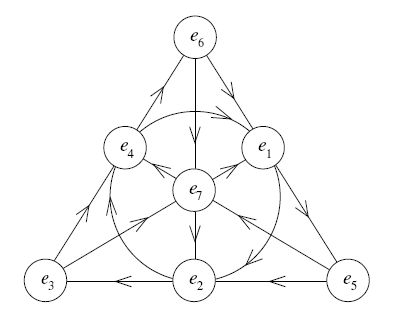
\includegraphics[max width=0.65\linewidth]{../images/fano.jpg}\] There
are 6 straight lines and a circle here: we call these all ``lines'', and
call this gadget the ``Fano plane''. There are 7 points and 7 lines:
each point lies on 3 lines, and each line goes through 3 points\ldots{}
very nice.

I won't describe how to use this picture to multiply octonions, since I
already did that in \protect\hyperlink{week104}{``Week 104''}, and we
won't need that here.

Now let me describe the Cayley integral octonions. I'll actually
describe all 240 of them that have length \(1\). Integer linear
combinations of these give the Cayley integral octonions --- or in other
words, a rescaled version of the \(\mathrm{E}_8\) lattice.

First, we include \(\pm e_i\) for \(i=0,\ldots,7\). Second, we include
\[\frac{\pm 1 \pm e_i \pm e_j \pm e_k}{2}\] whenever \(e_i\), \(e_j\)
and \(e_k\) are imaginary octonions that all lie on the same line in the
above chart. Third, we include
\[\frac{\pm e_i \pm e_j \pm e_k \pm e_l}{2}\] whenever \(e_i\), \(e_j\),
\(e_k\) and \(e_l\) are imaginary octonions that all lie \emph{off} the
same line in the above chart.

It's easy to see that all these octonions have length \(1\). It's also
easy to count them! There are \(2\times8 = 16\) of the first form,
\(2^4\times7 = 112\) of the second form, and \(2^4\times7 = 112\) of the
third form, for a total of 240.

It's harder to check that these 240 guys are closed under
multiplication. You can save some work by noticing that each line in the
Fano plane gives a copy of the quaternions sitting inside the octonions.
Moreover, the 24 quaternions of the form
\[\pm1,\quad \pm i,\quad \pm j,\quad \pm k,\quad \frac{\pm 1 \pm i \pm j \pm k}{2}\]
are closed under multiplication --- these are just the unit vectors
among the ``Hurwitz integral quaternions'', which form a
\(\mathrm{D}_4\) lattice in the quaternions (see
\protect\hyperlink{week91}{``Week 91''}). So, each line in the Fano
plane gives a copy of the integral quaternions sitting inside the
integral octonions. Even better --- I'm sorry, this is getting a bit
technical, but I need to write it down or I'll forget! --- if we do the
Cayley-Dickson construction (see \protect\hyperlink{week59}{``Week
59''}) to any of these copies of the integral quaternions, we get a
bigger set of integral octonions that's also closed under addition and
multiplication. Unfortunately, this bunch is just a copy of
\(\mathrm{D}_4 \times \mathrm{D}_4\) sitting inside \(\mathrm{E}_8\),
not the whole \(\mathrm{E}_8\). \(\mathrm{E}_8\) is the union of all
these \(\mathrm{D}_4 \times \mathrm{D}_4\)'s, one for line in the Fano
plane. So, I have to calculate more to finish convincing myself that the
Cayley integral octonions are closed under multiplication --- or
equivalently, that the 240 guys listed above are closed under
multiplication.

{[}Note: I later realized that they are \emph{not} closed under
multiplication! We have a perfectly fine \(\mathrm{E}_8\) lattice, so
everything that follows is okay\ldots{} but it's not the Cayley integral
octonions! I'll explain this next week.{]}

Anyway: this probably makes no sense to you, but \emph{I'm} happy as a
clam! So what can I do with them, for example?

Well, I can see some ways to make \(\mathrm{E}_8\) into a \emph{graded}
Lie algebra!

I guess I should start by saying some general stuff about graded Lie
algebras, which explains why this is interesting.

For starters, I'm not talking about \(\mathbb{Z}/2\)-graded Lie
algebras, also known as ``Lie superalgebras''; I'm talking about taking
a plain old Lie algebra \(L\) and writing it as a direct sum of
subspaces \(L(i)\), one for each integer \(i\), such that
\[\mbox{$[L(i), L(j)]$ is contained in $L(i+j)$.}\] If only the middle 3
of these subspace are nonzero, like so:
\[L = L(-1) \oplus L(0) \oplus L(1)\] we say \(L\) is ``\(3\)-graded''.
If only the middle 5 are nonzero, like so:
\[L = L(-2) \oplus L(-1) \oplus L(0) \oplus L(1) \oplus L(2)\] we say
\(L\) is ``\(5\)-graded''. And so on. In these situations, some nice
things happen.

First of all, \(L(0)\) is always a Lie subalgebra of \(L\). Second of
all, it acts on each other space \(L(i)\) by means of the bracket. Third
of all, if \(L\) is \(3\)-graded, we can give \(L(1)\) a product by
picking any element \(k\) of \(L(-1)\) and defining
\[x \circ y = [[x,k],y]\] This product automatically satisfies two of
identities defining a Jordan algebra:

\begin{itemize}
\tightlist
\item
  \(x \circ y = y \circ x\)
\item
  \(x \circ ((x \circ x) \circ y) = (x \circ x) \circ (x \circ y)\)
\end{itemize}

so \(3\)-graded Lie algebras are a great source of Jordan algebras.
Fourth of all, in this situation \(L(0)\) acts on \(L(1)\) by means of
the bracket operation, so we get a Lie algebra of ``infinitesimal
symmetries'' of our Jordan algebra, too. Fifth of all, if \(L\) is
\(5\)-graded, we get a more fancy algebraic structure called a ``Kantor
triple system'', but I'm not ready to talk about these, and you're
probably not ready to listen, either!

There's a lot more to say about this stuff, but let's just see a bit
about how it works for \(\mathrm{E}_8\). We've got two nice pictures of
the 240 roots of the \(\mathrm{E}_8\) lattice; you should imagine these
as the dazzling vertices of a beautiful diamond in 8 dimensions. To get
a grading on \(\mathrm{E}_8\), all we need to do is slice this diamond
with evenly spaced parallel hyperplanes in such a way that each vertex
of the diamond, as well as its center, lies on one of these hyperplanes.
There are different ways to do this, so you should imagine yourself as a
gem cutter, turning around this diamond, looking for nice ways to slice
it.

For example, if we use our picture of the \(\mathrm{E}_8\) lattice as
\(8\)-tuples that sum to an even integer are either all integers or all
half-integers, one obvious way to slice the diamond is to let each slice
go through those roots where the first coordinate takes on some fixed
value. The first coordinate can be \(1\), \(1/2\), \(0\), \(-1/2\), or
\(-1\), so we get a \(5\)-grading. Let's work out how many roots there
are of each kind:

\begin{itemize}
\tightlist
\item
  The number of roots with a ``\(1\)'' as the first component is
  \(7 + 7 = 14\).
\item
  The number of roots with a ``\(1/2\)'' as the first component is
  \(1 + \binom75 + \binom73 + \binom71 = 1 + 21 + 35 + 7 = 64\).
\item
  The number of roots with a ``\(0\)'' as the first component is \(84\).
\item
  The number of roots with a ``\(-1/2\)'' as the first component is
  \(1 + \binom75 + \binom73 + \binom71 = 1 + 21 + 35 + 7 = 64\).
\item
  The number of roots with a ``\(-1\)'' as the first component is
  \(7 + 7 = 14\).
\end{itemize}

Since I'm lazy, I figured out the number of roots with a ``\(0\)'' as
the first component by totalling up all the rest and subtracting that
from 240. That's how I got the number 84.

Now, whenever you have a simple Lie algebra it's a direct sum of ``root
spaces'', one for each root, together with an \(n\)-dimensional subspace
called the Cartan algebra, where \(n\) is the called the ``rank'' of the
Lie algebra. The rank of \(\mathrm{E}_8\) is 8, so its dimension is
\(240 + 8 = 248\). When we taking our way of slicing the diamond and
convert it into a grading of \(\mathrm{E}_8\), the roots in the \(i\)th
slice form a basis of \(L(i)\), except we also have to count the Cartan
as part of \(L(0)\). Thus in this example the dimension of \(L(0)\) is
not just \(84\) but \(84 + 8 = 92\). Some basic stuff about simple Lie
algebra guarantees that this trick always works: we get
\[\mbox{$[L(i), L(j)]$ is contained in $L(i+j)$}\] as desired.

So, in this example we get a \(5\)-grading where \[
  \begin{array}{ccccccccccc}
    \mathrm{E}_8 &= &L(-2) &\oplus &L(-1) &\oplus &L(0) &\oplus &L(1) &\oplus &L(2)
  \\248 &= &114 &+ &64 &+ &92 &+ &64 &+ &14
  \end{array}
\] where I'm writing the dimension of each vector space direct below it.

Now, \(L(0)\) is a Lie algebra, but which one? To figure this out we
need to think about how this diamond-cutting trick worked. At least in
this case --- and in fact it often works like this --- the roots in the
\(0\)th slice are just the roots of a simple Lie algebra of rank one
less than the one we started with. Since the Cartan of this smaller Lie
algebra is one dimension smaller, it turns out that \(L(0)\) equals this
smaller Lie algebra plus a one-dimensional abelian subalgebra --- namely
\(\mathfrak{u}(1)\).

In this example this smaller Lie algebra is \(\mathfrak{so}(14)\), which
has dimension 91. \(L(1)\) is a \(64\)-dimensional chiral spinor rep of
\(\mathfrak{so}(14)\), and \(L(2)\) is the \(14\)-dimensional vector
rep\ldots{} and similarly for \(L(-1)\) and \(L(-2)\). So we get a very
``14-dimensional'' picture of \(\mathrm{E}_8\):
\[\mathrm{E}_8 = [\mbox{vectors}] \oplus [\mbox{spinors}] \oplus [\mathfrak{so}(14) \oplus \mathfrak{u}(1)] \oplus [\mbox{spinors}] \oplus [\mbox{vectors}]\]
But we get a more exciting way of slicing the diamond if we use the
picture of \(\mathrm{E}_8\) as the Cayley integral octonions! Let's do
this, and let each slice go through those roots where the ``real part''
\(x_0\) of our octonion \[x_0 + x_1 e_1 + \ldots + x_7 e_7\] takes on
some fixed value. This value can be \(1\), \(1/2\), \(0\), \(-1/2\), or
\(-1\), so we again get a \(5\)-grading. Let's count the number of roots
in each slice:

\begin{itemize}
\tightlist
\item
  The number of roots with real part \(1\) is 1.
\item
  The number of roots with real part \(1/2\) is 56.
\item
  The number of roots with real part \(0\) is 126.
\item
  The number of roots with real part \(-1/2\) is 56.
\item
  The number of roots with real part \(-1\) is 1.
\end{itemize}

Here I got 56 roots with real part \(1/2\) by multiplying the number of
lines in the Fano plane by the number of sign choices in
\[{1 \pm e_i \pm e_j \pm e_k}{2}\] Similarly for the roots with real
part \(-1/2\). I got 126 roots with real part \(0\) by subtracting all
the other numbers on my list from 240.

So, we get a \(5\)-grading of \(\mathrm{E}_8\) like this: \[
  \begin{array}{ccccccccccc}
    \mathrm{E}_8 &= &L(-2) &\oplus &L(-1) &\oplus &L(0) &\oplus &L(1) &\oplus &L(2)
  \\248 &= &1 &+ &56 &+ &134 &+ &56 &+ &1
  \end{array}
\] since \(126 + 8 = 134\).

This shows how to get \(\mathrm{E}_8\) to act on a \(57\)-dimensional
manifold: we form the group \(\mathrm{E}_8\), and form the subgroup
\(G\) whose Lie algebra is \(L(-2) \oplus L(-1) \oplus L(0)\), and the
quotient \(\mathrm{E}_8/G\) will be a 57-dimensional space on which
\(\mathrm{E}_8\) acts! In fact this space is the smallest
``Grassmannian'' of \(\mathrm{E}_8\), as explained in
\protect\hyperlink{week181}{``Week 181''} --- look at the picture of the
\(\mathrm{E}_8\) Dynkin diagram near the end.

My goal in life is now to define a set of algebraic varieties, one for
each root in \(L(1)\) and \(L(2)\), so I can write a paper entitled ``57
Varieties'' and get sued for trademark infringement by Heinz.

In the above grading of \(\mathrm{E}_8\), the Lie algebra \(L(0)\) is
the direct sum of \(\mathrm{E}_7\) and \(\mathfrak{u}(1)\). This is no
surprise if you know that the dimension of \(\mathrm{E}_7\) is
133\ldots{} but the reason it's \emph{true} is that if you take the
roots of \(\mathrm{E}_8\) that are orthogonal to any one root, you get
the roots of \(\mathrm{E}_7\). So, we get a very \(\mathrm{E}_7\)-ish
description of \(\mathrm{E}_8\):
\[E8 = [\mbox{trivial}] \oplus [\mbox{Freudenthal}] \oplus [\mathrm{E}_7 \oplus \mathfrak{u}(1)] \oplus [\mbox{Freudenthal}] \oplus [\mbox{trivial}]\]

Here the ``Freudenthal algebra'' is the \(56\)-dimensional irrep of
\(\mathrm{E}_7\), which has an invariant symplectic structure and
ternary product satisfying some funky equations which get turned into
the definition of\ldots{} a Freudenthal algebra!

There are a lot of other games we can play like this, but like solitaire
they're not too fun to watch, so I'll just mention one more, and then
give a bunch more references.

Above we have seen the roots of \(\mathrm{E}_7\) as the imaginary Cayley
integral octonions of norm \(1\). These form a \(7\)-dimensional
gemstone with 126 vertices, and we can repeat the same ``gem-slicing''
trick on a smaller scale to get gradings of the Lie algebra
\(\mathrm{E}_7\). If we do this in a nice way, we get a \(3\)-grading of
\(\mathrm{E}_7\): \[
  \begin{array}{ccccccc}
    \mathrm{E}_7 &= &L(-1) &\oplus &L(0) &\oplus &L(1)
  \\133 &= &27 &+ &79 &+ &727
  \end{array}
\] Since \(\mathrm{E}_7\)'s baby brother \(\mathrm{E}_6\) is
\(78\)-dimensional, it's no surprise that the Lie algebra \(L(0)\) is
\(\mathrm{E}_6\oplus\mathfrak{u}(1)\). Since \(3\)-gradings tend to give
us Jordan algebras, it's no suprise that \(L(1)\) is the exceptional
Jordan algebra \(\mathrm{h}_3(\mathbb{O})\) consisting of all
\(3\times3\) hermitian octonionic matrices. \(\mathrm{E}_6\) acts as the
group of all transformations of \(\mathrm{h}_3(\mathbb{O})\) preserving
the determinant, and in fact \(\mathrm{h}_3(\mathbb{O})\) is an irrep of
\(\mathrm{E}_6\). \(L(-1)\) is just the dual of this rep. So, we get a
very octonionic description of \(\mathrm{E}_7\):
\[E7 = \mathrm{h}_3(\mathbb{O})^* \oplus [\mathrm{E}_6 \oplus \mathfrak{u}(1)] \oplus \mathrm{h}_3(\mathbb{O}).\]

Now, since \(\mathrm{E}_6\) sits in \(\mathrm{E}_7\) which sits in
\(\mathrm{E}_8\), just like nested Russian dolls, we can take our
previous description of \(\mathrm{E}_8\):
\[E8 = [\mbox{trivial}] \oplus [\mbox{Freudenthal}] \oplus [\mathrm{E}_7 \oplus \mathfrak{u}(1)] \oplus [\mbox{Freudenthal}] \oplus [\mbox{trivial}]\]
and decompose everything in sight as irreps of \(\mathrm{E}_6\). If we
do this, the only new exciting thing that happens is that the
Freudenthal algebra decomposes into a copy of the exceptional Jordan
algebra, a copy of its dual, and two copies of the trivial rep:
\[[\mbox{Freudenthal}] = [\mbox{trivial}] \oplus \mathrm{h}_3(\mathbb{O})* \oplus \mathrm{h}_3(\mathbb{O}) \oplus [\mbox{trivial}]\]
At least I \emph{think} this is right: people sometimes write elements
of the Freudenthal algebra as \(2\times2\) matrices
\[\left(\begin{array}{cc}a&x\\y&b\end{array}\right)\] where \(a,b\) are
real and \(x,y\) lie in \(\mathrm{h}_3(\mathbb{O})\), but I suspect
they're ``cheating'' a bit and identifying \(\mathrm{h}_3(\mathbb{O})\)
with its dual.

In short, \(\mathrm{E}_8\) contains a lot of other ``exceptional''
structures, all arranged in a very nice way.

Now for some references and apologies.

I didn't do justice to the stuff about Jordan algebras and \(3\)-graded
Lie algebras, because I'm still confused about certain aspects. For
example, where does the unit in the Jordan algebra come from? I also
didn't explain precisely what sort of ``infinitesimal symmetries'' we
get from the action of \(L(0)\) on \(L(1)\). If we exponentiate these
infinitesimal symmetries, we don't usually get automorphisms of
\(L(1)\), since there's no reason for the element ``\(k\)'' to be
preserved --- remember that \[x \circ y = [[x,k],y]\]

Instead, we get transformations that tend to preserve a ``determinant''
on \(L(1)\). People call \(L(0)\) the ``structure algebra'' of \(L(1)\)
and call the corresponding group the ``structure group''. There's a
pretty readable explanation here:

\begin{enumerate}
\def\labelenumi{\arabic{enumi})}
\setcounter{enumi}{3}
\tightlist
\item
  Kevin McCrimmon, ``Jordan Algebras and their applications'',
  \emph{Bull. AMS} \textbf{84} (1978) 612--627.
\end{enumerate}

and hopefully even more here:

\begin{enumerate}
\def\labelenumi{\arabic{enumi})}
\setcounter{enumi}{4}
\tightlist
\item
  Kevin McCrimmon, A \emph{Taste of Jordan Algebras}, Springer, Berlin,
  perhaps to appear in March 2003. Available for free online at
  \texttt{http://math1.uibk.ac.at/mathematik/jordan/archive/atoja/} ---
  but watch out, it's 545 pages long!
\end{enumerate}

In fact, all this is part of a bigger relationship between \(3\)-graded
Lie algebras and so-called ``Jordan triple systems'' known as the
Tits-Kantor-Koecher construction. Jordan triple systems are a
generalization of Jordan algebras --- and I'm sort of confused about why
this generalization also turns up here. I guess I should read these too:

\begin{enumerate}
\def\labelenumi{\arabic{enumi})}
\setcounter{enumi}{5}
\item
  J. Tits, ``Une class d'algebres de Lie en relations avec les algebres
  de Jordan'', \emph{Ned. Akad. Wet., Proc. Ser. A} \textbf{65} (1962),
  530.
\item
  M. Koecher, ``Imbedding of Jordan algebras into Lie algebra I'',
  \emph{Am. J. Math.} \textbf{89} (1967), 787.
\item
  Soji Kaneyuki, ``Graded Lie algebras, related geometric structures,
  and pseudo-hermitian symmetric spaces'', in \emph{Analysis and
  Geometry on Complex Homogeneous Domains}, by Faraut, Kaneyuki,
  Koranyi, Lu, and Roos, Birkhauser, New York, 2000.
\end{enumerate}

Kaneyuki has made some nice tables of \(3\)-gradings on simple Lie
algebras, and you can see some of these here:

\begin{enumerate}
\def\labelenumi{\arabic{enumi})}
\setcounter{enumi}{8}
\tightlist
\item
  Tony Smith, ``Graded Lie algebras'',
  \texttt{http://www.innerx.net/personal/tsmith/GLA.html}
\end{enumerate}

Thomas Larsson has made a nice table of all the formally real simple
Jordan algebras you get from \(3\)-graded simple Lie algebras, and here
it is, slightly modified:

\begin{longtable}[]{@{}llll@{}}
\toprule
\begin{minipage}[b]{0.22\columnwidth}\raggedright
Lie algebra \(L\)\strut
\end{minipage} & \begin{minipage}[b]{0.18\columnwidth}\raggedright
\(L'(0)\)\strut
\end{minipage} & \begin{minipage}[b]{0.18\columnwidth}\raggedright
\(\dim(L(1))\)\strut
\end{minipage} & \begin{minipage}[b]{0.31\columnwidth}\raggedright
Jordan algebra \(L(1)\)\strut
\end{minipage}\tabularnewline
\midrule
\endhead
\begin{minipage}[t]{0.22\columnwidth}\raggedright
\(\mathfrak{sl}(n+1)\)\strut
\end{minipage} & \begin{minipage}[t]{0.18\columnwidth}\raggedright
\(\mathfrak{sl}(n)\)\strut
\end{minipage} & \begin{minipage}[t]{0.18\columnwidth}\raggedright
\(n\)\strut
\end{minipage} & \begin{minipage}[t]{0.31\columnwidth}\raggedright
\(\mathbb{R}^{n-1}\oplus\mathbb{R}\)\strut
\end{minipage}\tabularnewline
\begin{minipage}[t]{0.22\columnwidth}\raggedright
\(\mathfrak{so}(n+2)\)\strut
\end{minipage} & \begin{minipage}[t]{0.18\columnwidth}\raggedright
\(\mathfrak{so}(n)\)\strut
\end{minipage} & \begin{minipage}[t]{0.18\columnwidth}\raggedright
\(n\)\strut
\end{minipage} & \begin{minipage}[t]{0.31\columnwidth}\raggedright
\(\mathbb{R}^{n-1}\oplus\mathbb{R}\)\strut
\end{minipage}\tabularnewline
\begin{minipage}[t]{0.22\columnwidth}\raggedright
\(\mathfrak{sp}(2n)\)\strut
\end{minipage} & \begin{minipage}[t]{0.18\columnwidth}\raggedright
\(\mathfrak{sl}(n)\)\strut
\end{minipage} & \begin{minipage}[t]{0.18\columnwidth}\raggedright
\((n^2+n)/2\)\strut
\end{minipage} & \begin{minipage}[t]{0.31\columnwidth}\raggedright
\(\mathrm{h}_n(\mathbb{R})\)\strut
\end{minipage}\tabularnewline
\begin{minipage}[t]{0.22\columnwidth}\raggedright
\(\mathfrak{so}(2n)\)\strut
\end{minipage} & \begin{minipage}[t]{0.18\columnwidth}\raggedright
\(\mathfrak{sl}(n)\)\strut
\end{minipage} & \begin{minipage}[t]{0.18\columnwidth}\raggedright
\((n^2-n)/2\)\strut
\end{minipage} & \begin{minipage}[t]{0.31\columnwidth}\raggedright
\(\mathrm{h}_{n-1}(\mathbb{R})\)\strut
\end{minipage}\tabularnewline
\begin{minipage}[t]{0.22\columnwidth}\raggedright
\(\mathfrak{sl}(2n)\)\strut
\end{minipage} & \begin{minipage}[t]{0.18\columnwidth}\raggedright
\(\mathfrak{sl}(n)+\mathfrak{sl}(n)\)\strut
\end{minipage} & \begin{minipage}[t]{0.18\columnwidth}\raggedright
\(n^2\)\strut
\end{minipage} & \begin{minipage}[t]{0.31\columnwidth}\raggedright
\(\mathrm{h}_n(\mathbb{C})\)\strut
\end{minipage}\tabularnewline
\begin{minipage}[t]{0.22\columnwidth}\raggedright
\(\mathfrak{so}(4n)\)\strut
\end{minipage} & \begin{minipage}[t]{0.18\columnwidth}\raggedright
\(\mathfrak{sl}(2n)\)\strut
\end{minipage} & \begin{minipage}[t]{0.18\columnwidth}\raggedright
\(2n^2-n\)\strut
\end{minipage} & \begin{minipage}[t]{0.31\columnwidth}\raggedright
\(\mathrm{h}_n(\mathbb{H})\)\strut
\end{minipage}\tabularnewline
\begin{minipage}[t]{0.22\columnwidth}\raggedright
\(\mathrm{E}_7\)\strut
\end{minipage} & \begin{minipage}[t]{0.18\columnwidth}\raggedright
\(\mathrm{E}_6\)\strut
\end{minipage} & \begin{minipage}[t]{0.18\columnwidth}\raggedright
\(27\)\strut
\end{minipage} & \begin{minipage}[t]{0.31\columnwidth}\raggedright
\(\mathrm{h}_3(\mathbb{O})\)\strut
\end{minipage}\tabularnewline
\begin{minipage}[t]{0.22\columnwidth}\raggedright
\(\mathrm{E}_6\)\strut
\end{minipage} & \begin{minipage}[t]{0.18\columnwidth}\raggedright
\(\mathfrak{so}(10)\)\strut
\end{minipage} & \begin{minipage}[t]{0.18\columnwidth}\raggedright
\(16\)\strut
\end{minipage} & \begin{minipage}[t]{0.31\columnwidth}\raggedright
\(\mathrm{h}_4(\mathbb{C})\)\strut
\end{minipage}\tabularnewline
\bottomrule
\end{longtable}

Since \(L(0)\) always contains a \(\mathfrak{u}(1)\) summand in these
cases, we write \[L(0) = L'(0) + \mathfrak{u}(1)\] so that \(L'(0)\) is
the interesting part of \(L(0)\). The formally real simple Jordan
algebras appearing here are all those listed in
\protect\hyperlink{week162}{``Week 162''} --- we get all of them! In
particular, \(\mathbb{R}^{n-1}\oplus\mathbb{R}\) is the so-called ``spin
factor'' Jordan algebra, which appears in special relativity.

For the more intricate relationship between \(5\)-graded Lie algebras,
Freudenthal algebras and Kantor triple systems, I should reread these:

\begin{enumerate}
\def\labelenumi{\arabic{enumi})}
\setcounter{enumi}{9}
\item
  I. Kantor, I. Skopets, ``Some results on Freudenthal triple systems'',
  \emph{10el. Math. Sov.} \textbf{2} (1982), 293.
\item
  K. Meyberg, ``Eine Theorie Der Freudenthalschen Tripelsysteme, I,
  II'', \emph{Ned. Akad. Wet., Proc. Ser. A} \textbf{71} (1968),
  162--190.
\item
  R. Skip Garibaldi, Structurable algebras and groups of types
  \(\mathrm{E}_6\) and \(\mathrm{E}_7\), available at
  \href{http://www.arXiv.org/abs/math.RA/9811035}{\texttt{math.RA/9811035}}.
\item
  R. Skip Garibaldi, ``Groups of type \(\mathrm{E}_7\) over arbitrary
  fields'', available at
  \href{http://www.arXiv.org/abs/math.RA/9811056}{\texttt{math.RA/9811056}}.
\item
  G. Sierra, ``An application of the theories of Jordan algebras and
  Freudenthal triple systems to particles and strings'', \emph{Class.
  Quant. Grav.} \textbf{4} (1987), 227--236.
\end{enumerate}

Also, I didn't say anything yet about the connection of Lie triple
systems, Jordan algebras, and Jordan triple systems to the geometry of
symmetric spaces! There is in fact a dictionary relating these funny
algebraic structures to very nice kinds of geometry, which motivates the
Tits-Kantor-Koecher construction and its generalizations. Someday I may
understand this well enough to explain it. For now, you should try to
get ahold of these:

\begin{enumerate}
\def\labelenumi{\arabic{enumi})}
\setcounter{enumi}{14}
\item
  W. Bertram, \emph{The Geometry of Jordan and Lie structures}, Lecture
  Notes in Mathematics \textbf{1754}, Springer, Berlin, 2001.
\item
  Ottmar Loos, ``Jordan triple systems, \(R\)-spaces and bounded
  symmetric domains'', \emph{Bull. AMS} \textbf{77} (1971), 558--561.
\item
  Ottmar Loos, \emph{Symmetric Spaces I: General Theory}, W. A.
  Benjamin, New York, 1969. \emph{Symmetric Spaces II: Compact Spaces
  and Classification}, W. A. Benjamin, New York, 1969.
\end{enumerate}

Unfortunately of the last two books I can get only volume I at U.C.
Riverside, and only volume II here at Macquarie University! Someone
should reprint both of these books: they're nice. Loos has also written
a book on ``Jordan pairs'', but in my current state of development I
find that unreadable.

\begin{center}\rule{0.5\linewidth}{0.5pt}\end{center}

\textbf{Addendum:} Blichfeldt proved in 1935 that \(\mathrm{E}_8\) is a
maximally dense lattice packing of spheres in 8 dimensions, and
Vetcinkin proved in 1980 that it's the \emph{unique} lattice packing
that achieves this density in 8 dimensions. Now Cohn and Kumar have
shown that the \(\mathrm{E}_8\) packing is darn close to the densest of
\emph{all} sphere packings in 8 dimensions, lattice or not. No other can
be more than \(1+10^{-14}\) as dense as this one!

They also showed that in 24 dimensions no packing can be more than
\(1+10^{-29}\) times as dense as the Leech lattice, and that this is the
unique best lattice packing. Of course the \(\mathrm{E}_8\) and Leech
lattices are probably the best of all sphere packings in their
dimensions, but it's very hard to understand the set of all sphere
packings, so even these partial results are amazing.

Here are their papers:

\begin{enumerate}
\def\labelenumi{\arabic{enumi})}
\setcounter{enumi}{17}
\item
  H. Cohn and A. Kumar, ``Optimality and uniqueness of the Leech lattice
  among lattices'', available at
  \href{http://www.arxiv.org/abs/math.MG/0403263}{\texttt{math.MG/0403263}}.

  H. Cohn and A. Kumar, ``The densest lattice in twenty-four
  dimensions'', \emph{Elec. Res. Ann.} \textbf{10} (2004), 58--67.
  Available online at
  \texttt{http://www.ams.org/era/2004-10-07/S1079-6762-04-00130-1/home.html}
\end{enumerate}

There's also a really nice overview of this topic in the American
Mathematical Society Notices, which explains how people manage to prove
results about \emph{all} packings:

\begin{enumerate}
\def\labelenumi{\arabic{enumi})}
\setcounter{enumi}{18}
\tightlist
\item
  Florian Pfender and Günter M. Ziegler, ``Kissing numbers, sphere
  packings, and some unexpected proofs'', \emph{AMS Notices} \textbf{51}
  (September 2004), 873--883. Available online at
  \texttt{http://www.ams.org/notices/200408/200408-toc.html}
\end{enumerate}

And while you're at it, read this article, which studies a question
mentioned in \protect\hyperlink{week20}{``Week 20''}:

\begin{enumerate}
\def\labelenumi{\arabic{enumi})}
\setcounter{enumi}{19}
\tightlist
\item
  Bill Casselman, ``The difficulties of kissing in three dimensions'',
  \emph{AMS Notices} \textbf{51} (September 2004), 884--885. Available
  online at \texttt{http://www.ams.org/notices/200408/200408-toc.html}
\end{enumerate}

namely, how to roll twelve balls in 3 dimensions around the surface of a
thirteenth ball of equal size.

\begin{center}\rule{0.5\linewidth}{0.5pt}\end{center}

\begin{quote}
\emph{The essential thing was that Serre each time strongly sensed the
rich meaning behind a statement that, on the page, would doubtless have
left me neither hot nor cold --- and that he could ``transmit'' this
perception of a rich, tangible and mysterious substance --- this
perception that is at the same time the \textbf{desire} to understand
this substance, to penetrate it.}
\end{quote}

--- Alexandre Grothendieck, \emph{Récoltes et Semailles}, p.~556.



\hypertarget{week194}{%
\section{March 17, 2003}\label{week194}}

I recently flew from Sydney, Australia to Waterloo, Canada. All of a
sudden day became night and steamy \(30\) Celsius summertime suddenly
switched to a \(-15\) Celsius blizzard. Unsurprisingly, I came down with
a cold. Nonetheless, I'm very happy to be here. I'm visiting the
Perimeter Institute of Theoretical Physics, seeing old friends like
Louis Crane, Fotini Markopoulou and Lee Smolin, and newer ones like
Laurent Freidel, Hendryk Pfeiffer and Olaf Dreyer. There's a lot of
interesting gossip about quantum gravity, string theory\ldots.

But more about that later! Now I want to talk about Conway's new book.

Last week I described what I \emph{thought} were the Cayley integral
octonions. But then Dan Piponi showed me that I had screwed up: they
aren't closed under multiplication. I was very confused until I arrived
here.

On the day I showed up, I got a packet of mail containing this book:

\begin{enumerate}
\def\labelenumi{\arabic{enumi})}
\tightlist
\item
  John H. Conway and Derek A. Smith, \emph{On Quaternions and Octonions:
  Their Geometry, Arithmetic, and Symmetry}, A. K. Peters, Ltd., Natick,
  Massachusetts, 2003.
\end{enumerate}

Conway and Smith sent it to me because they quoted my history of the
octonions. And in this book, there is a description of my mistake and
how to fix it! They attribute it to someone named J. Kirmse, and write:

\begin{quote}
Other people have made this very natural assumption, so it is convenient
that it has a standard name: ``Kirmse's Mistake.'' The product of two
Kirmse integers happens to be a Kirmse integer rather more than one
third of the time.
\end{quote}

There's nothing like getting your mistake corrected by a book in the
mail from Conway! Many of you probably know him for his work on surreal
numbers and the game of Life. Among mathematicians he's famous for his
work on game theory, the Leech lattice and finite simple groups. He's
also famous for acting like he just quantum-tunnelled out of a Lewis
Carroll novel. If you don't know what I mean, you're missing out on a
\emph{lot} of fun\ldots{} so you should immediately read this:

\begin{enumerate}
\def\labelenumi{\arabic{enumi})}
\setcounter{enumi}{1}
\tightlist
\item
  Charles Seife, ``Mathemagician (impressions of Conway)'', \emph{The
  Sciences} (May/June 1994), 12--15. Available at
  \texttt{http://www.users.cloud9.net/\textasciitilde{}cgseife/conway.html}
\end{enumerate}

Just to entice you, I'll quote the beginning:

\begin{quote}
``Have I done this to you yet?'' He grabbed my hand and held it out in
front of him, palm down. Before I could react, he pulled a rubber stamp
out of his pocket, and my hand suddenly was emblazoned with big red
letters. ``John H. Conway's Seal of Grudging Approval.'' Within seconds,
it had smeared to three red lines that wouldn't wash off for several
days. Still grasping my hand, he pulled me toward his office. Brightly
colored polyhedra hung in disarray from a network of strings dangling
from the ceiling. The dim outline of a computer terminal was visible
through a pile of Rubik's cubes and wooden toroids. ``We'll be better
off in the undergraduate lounge. The doctor says I should rest, and I
can lie down over there.''
\end{quote}

Anyway, he's been busy writing books lately. Not too long ago, he
finished one about the classification of quadratic forms:

\begin{enumerate}
\def\labelenumi{\arabic{enumi})}
\setcounter{enumi}{2}
\tightlist
\item
  John H. Conway and Francis Fung, \emph{The Sensual (Quadratic) Form},
  Mathematical Association of America, Washington DC, 1997.
\end{enumerate}

and before that, a very fun elementary one about numbers:

\begin{enumerate}
\def\labelenumi{\arabic{enumi})}
\setcounter{enumi}{3}
\tightlist
\item
  John H. Conway and Richard K. Guy, \emph{The Book of Numbers},
  Copernicus, New York, 1996.
\end{enumerate}

Now he's into quaternions and octonions. But his new book with Derek
Smith starts by talking about the real numbers and \(1\)-dimensional
geometry. Then it turns to complex numbers and \(2\)-dimensional
geometry, including the Gaussian and Eisenstein integers and the 17
``space groups'' in 2 dimensions.

Perhaps I should say what these things are. The Gaussian integers are
complex numbers of the form \[a + bi\] where \(a\) and \(b\) are
integers. They form a square lattice: \[
  \begin{tikzpicture}[scale=0.7]
    \draw[->] (-2.5,0) to (4,0) node[label=below:{$\Re(z)$}]{};
    \draw[->] (0,-2) to (0,4) node[label=left:{$\Im(z)$}]{};
    \foreach \m in {-1,0,1,2}
    {
      \foreach \n in {-1,0,1,2}
      {
        \node at ({1.5*\m},{1.6*\n}) {$\bullet$};
      }
    }
  \end{tikzpicture}
\] You can uniquely factor any Gaussian integer into primes --- at least
if you count differently ordered factorizations as the same, and ignore
the ambiguity due to ``units'' --- the invertible Gaussian integers
\(1\), \(i\), \(-1\), and \(-i\). You can prove this using the geometry
of the square lattice\ldots{} for details, read the book!

The Eisenstein integers are complex numbers of the form \[a + bw\] where
\(a\) and \(b\) are integers and \(w\) is a nontrivial cube root of
\(-1\). These are closed under addition and multiplication, and they
form a lattice with hexagonal symmetry: \[
  \begin{tikzpicture}[scale=0.7]
    \draw[->] (-3,0) to (4.5,0) node[label=below:{$\Re(z)$}]{};
    \draw[->] (0,-2) to (0,3.5) node[label=left:{$\Im(z)$}]{};
    \foreach \m in {-1,0,1,2}
    {
      \foreach \n in {-1,0,1,2}
      {
        \node at ({1.5*\m+0.75*\n},{1.33*\n}) {$\bullet$};
      }
    }
  \end{tikzpicture}
\] Again you can use geometry to prove unique factorization up to
reordering and units.

The Gaussian and Eisenstein integers are the most symmetrical lattices
in 2 dimensions: they have \(4\)-fold and \(6\)-fold rotational
symmetry, respectively. As I explained in
\protect\hyperlink{week124}{``Week 124''} and subsequent Weeks, this is
related to the appearance of the number 24 in bosonic string theory. But
these lattices also play a role in crystallography, in the
classification of \(2\)-dimensional ``space groups''.

I'm not sure what the definition of a ``space group'' is --- the
references I've seen are annoyingly reticent on this point --- but it's
something like a subgroup of the Euclidean group (the group generated by
rotations, reflections and translations) that acts transitively on a
lattice. There are 17 space groups in 2 dimensions, also called
``wallpaper groups'' since they give different symmetries of repetitive
wallpaper patterns. Of these, 2 act on a lattice with no special
symmetry: \[
  \begin{tikzpicture}[scale=0.7]
    \draw[->] (-3,0) to (4.5,0) node[label=below:{$\Re(z)$}]{};
    \draw[->] (0,-2.25) to (0,3.5) node[label=left:{$\Im(z)$}]{};
    \foreach \m in {-1,0,1,2}
    {
      \foreach \n in {-1,0,1,2}
      {
        \node at ({1.5*\m-0.4*\n},{1.33*\n}) {$\bullet$};
      }
    }
  \end{tikzpicture}
\] 7 act on a lattice with rectangular symmetry: \[
  \begin{tikzpicture}[scale=0.7]
    \draw[->] (-3,0) to (4,0) node[label=below:{$\Re(z)$}]{};
    \draw[->] (0,-2) to (0,3) node[label=left:{$\Im(z)$}]{};
    \foreach \m in {-1,0,1,2}
    {
      \foreach \n in {-1,0,1,2}
      {
        \node at ({1.7*\m},{1.1*\n}) {$\bullet$};
      }
    }
  \end{tikzpicture}
\] or alternatively, on a lattice with rhombic symmetry: \[
  \begin{tikzpicture}[scale=0.7]
    \draw[->] (-3,0) to (4.5,0) node[label=below:{$\Re(z)$}]{};
    \draw[->] (0,-2.25) to (0,3.5) node[label=left:{$\Im(z)$}]{};
    \foreach \x in {-2,0,2}{
      \foreach \y in {-1,0,1,2}
        \node at (\x,\y) {$\bullet$};
    }
    \foreach \x in {-1,1,3}{
      \foreach \y in {-1.5,-0.5,0.5,1.5,2.5}
        \node at (\x,\y) {$\bullet$};
    }
  \end{tikzpicture}
\] 3 act on a lattice with square symmetry, and 5 act on a lattice with
hexagonal symmetry. For more details, with pictures, see:

\begin{enumerate}
\def\labelenumi{\arabic{enumi})}
\setcounter{enumi}{4}
\item
  NIST, ``The 17 two-dimensional space groups'',
  \texttt{http://www.nist.gov/srd/webguide/nist42-3/appa.htm}
\item
  Eric Weisstein, ``Wallpaper groups'',
  \texttt{http://mathworld.wolfram.com/WallpaperGroups.html}
\item
  David Hestenes, ``Point groups and space groups in geometric
  algebra'', \texttt{modelingnts.la.asu.edu/pdf/crystalsymmetry.pdf}
\end{enumerate}

After this low-dimensional warmup, Conway and Smith's book turns to the
quaternions and their applications to \(3\)-dimensional and
\(4\)-dimensional geometry. They classify the finite subgroups of the 3d
rotation group \(\mathrm{SO}(3)\), its double cover \(\mathrm{SU}(2)\),
and the 3d rotation/reflection group \(\mathrm{O}(3)\). They also
classify the finite subgroups of the 4d rotation group. They mention but
do not study the 230 space groups in 3 dimensions.

Then they turn to quaternionic number theory! The ``Lipschitz integral
quaternions'' are of the form \[a + bi + cj + dk\] where \(a,b,c,d\) are
integers. But number theory works better for the ``Hurwitz integral
quaternions'', which are of the form \[a + bi + cj + dk\] where
\(a,b,c,d\) are either all integers or all half-integers. These are
closed under addition and multiplication, and they form a lattice called
the \(\mathrm{D}_4\) lattice, which gives the densest lattice packing of
spheres in 4 dimensions --- each sphere has 24 nearest neighbors. They
prove a version of unique prime factorization for Hurwitz integral
quaternions. But the sense of ``uniqueness'' here is a lot more tricky,
in part because the quaternions are noncommutative.

Finally, they study the octonions. They start with a truly excellent
study of Moufang loops, isotopies and triality --- three fairly esoteric
subjects that are crucial for understanding octonions. Then they tackle
octonionic number theory! The ``Gravesian integral octonions'' are
octonions of the form
\[a_0 + a_1 e_1 + a_2 e_2 + a_3 e_3 + a_4 e_4 + a_5 e_5 + a_6 e_6 + a_7 e_7\]
where all the coefficients are integers. The ``Kleinian integral
octonions'' are those where the coefficients are either all integers or
all half-integers. Both these are closed under addition and
multiplication. To get even denser lattices closed under multiplication,
we need the octonion multiplication chart (see
\protect\hyperlink{week104}{``Week 104''}):
\[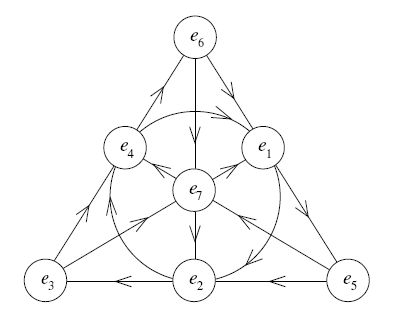
\includegraphics[max width=0.65\linewidth]{../images/fano.jpg}\] This
has 7 lines in it, if we count the circle containing \(e_1,e_2,e_4\) as
an honorary ``line''. To get the ``double Hurwitzian integral
octonions'', first pick one of these lines. Then, take all integral
linear combinations of Gravesian integral octonions, octonions of the
form \[\frac{\pm 1 \pm e_i \pm e_j \pm e_k}{2}\] where \(e_i\), \(e_j\),
\(e_k\) lie on this line, and those of the form
\[\frac{\pm e_i \pm e_j \pm e_k \pm e_l}{2}\] where \(e_i\), \(e_j\),
\(e_k\), and \(e_l\) all lie \emph{off} this line. We get 7 different
versions of the double Hurwitzian integral octonions this way. Each is
closed under addition and multiplication, and each is a copy of the
lattice called \(\mathrm{D}_4 \times \mathrm{D}_4\).

To get an even denser lattice, we can take the union of all 7 different
double Hurwitzian integral octonions. I talked about this last week. We
get an \(\mathrm{E}_8\) lattice, which gives the densest packing of
spheres in 8 dimensions --- each sphere has 240 nearest neighbors. I
\emph{thought} this lattice was closed under multiplication, but it's
not! Conway and Smith mockingly call it the ``Kirmse integral
octonions''.

To fix this problem, you need to perform a slight trick. Pick a number
\(i\) from 1 to 7. Then, take all the Kirmse integral octonions
\[a_0 + a_1 e_1 + a_2 e_2 + a_3 e_3 + a_4 e_4 + a_5 e_5 + a_6 e_6 + a_7 e_7\]
and switch the coefficients \(a_0\) and \(a_i\). Bizarrely, the
resulting ``Cayley integral octonions'' are closed under multiplication.
But they are still an \(\mathrm{E}_8\) lattice --- just a rotated
version of the Kirmse integral octonions.

Since this trick involved an arbitrary choice, there are 7 different
copies of the Cayley integral octonions containing the Gravesian
integral octonions. And this is as good as it gets: each one is maximal
in a certain sense which Conway and Smith explain. They study prime
factorization in the Cayley integral octonions, but it's very tricky,
since the octonions are nonassociative.

I've got a bunch more to talk about, but I've probably scared away
everybody except the octonion-heads, so I'll wait until next week. I'll
just mention this review article, which octonion-heads should enjoy:

\begin{enumerate}
\def\labelenumi{\arabic{enumi})}
\setcounter{enumi}{7}
\tightlist
\item
  B. S. Acharya, ``M theory, \(\mathrm{G}_2\) manifolds and
  four-dimensional physics'', \emph{Class. Quant. Grav.} \textbf{19}
  (2002), 5619--5653.
\end{enumerate}

It's nice because it goes all the way from the definition of a
\(\mathrm{G}_2\) manifold to (sketchy but readable) physical
considerations like the rate of proton decay.

\begin{center}\rule{0.5\linewidth}{0.5pt}\end{center}

\textbf{Addendum:} Tony Smith writes:

\begin{quote}
Thanks for mentioning the John Conway --- Derek Smith book in week 194.
I have ordered it from Amazon.

BTW --- ( and my apologies if you have already seen these details if
they are in the Conway-Smith book ) --- Kirmse's mistake is described in
some detail in Coxeter's paper ``Integral Cayley Numbers'' (\emph{Duke
Math. J.}, v. \textbf{13}, no. 4, December 1946), in which Coxeter says:
``\ldots{} Kirmse \ldots{} selects an eight-dimensional module \ldots{}
which is closed under subtraction and contains eight linearly
independent members. .. a module is called an INTEGRAL DOMAIN if it is
closed under multiplication. A simple instance is the module \(J_0\)
consisting of all Cayley numbers \ldots{} {[}that are{]} integers.
\ldots{} \ldots{} {[}Kirmse{]} then defines a maximal \ldots{} integral
domain over \(J_0\) as an extension of \(J_0\) which cannot be further
extended without ceasing to be an integral domain. He states that there
are EIGHT such domains, one of which he calls \(J_1\) and describes in
detail. Actually, there are only SEVEN, which presumably are the
remaining seven of his eight. \ldots{} \(J_1\) itself is not closed
under multiplication. \ldots{} Since the \(168\)-group is doubly
transitive on the seven {[}imaginary octonions{]}, ANY transposition
{[}of the imaginary octonions{]} will serve to rectify \(J_1\) in the
desired manner. But there are only seven such domains, since the
\((7|2) = 21\) possible transpositions fall into 7 sets of 3, each set
having the same effect. In each of the seven domains, one of the
{[}imaginary octonions{]} plays a special role, viz., that one which is
not affected by any of the three transpositions. Comparing Kirmse's
multiplication table with Cayley's \ldots{} we see that \ldots{}
Kirmse's \(J_1\) could be used as it stands if we replaced his
multiplication table with Cayley's. \ldots{}''

\begin{center}\rule{0.5\linewidth}{0.5pt}\end{center}

These integral domains are also discussed in Coxeter's paper ``Regular
and Semi-Regular Polyotpes III'' (\emph{Math. Z.} \textbf{200}, 3--45,
1988), where he describes the 240 units of an \(\mathrm{E}_8\) integral
domain as

"\ldots{} the \(16 + 16 + 16\) octaves \[1, i, j, k, e, ie, je, ke,\]
\[(1iejeke)/2,\] \[(eijk)/2,\] and the 192 others derived from the last
two expressions by cyclically permuting the 7 symbols
{[}\(i,j,k,e,ie,je,ke\){]} in the peculiar order
\[e, i, j, ie, ke, k, je\] \ldots{} It seems somewhat paradoxical
\ldots{} that the cyclic permutation \[( e, i, j, ie, ke, k, je ),\]
which preserves the integral domain (and the finite projective
{[}Fano{]} plane \ldots) is not an automorphism of the whole ring of
octaves; it transforms the associative triad \(ijk\) into the
anti-associative triad \(j ie je\).

On the other hand, the permutation \[( e ie je i k ke j ),\] which IS an
automorphism of the whole ring of octaves (and of the finite {[}Fano{]}
plane \ldots) transforms this particular integral domain into another
one of R. H. Bruck's cyclic of seven such domains. \ldots".

Tony

18 March 2003
\end{quote}

\begin{center}\rule{0.5\linewidth}{0.5pt}\end{center}

\begin{quote}
\emph{``Quaternions came from Hamilton after his really good work had
been done; and though beautifully ingenious, have been an unmixed evil
to those who have touched them in any way.''}

--- Lord Kelvin
\end{quote}



\hypertarget{week195}{%
\section{March 23, 2003}\label{week195}}

In 1999 a Canadian businessman named Mike Lazaridis donated \$100
million to set up the Perimeter Institute for Theoretical Physics. Right
now it's housed in a red stone building with a big clock tower on King
Street in Waterloo, Ontario. It's funky and comfortable: the place used
to be a restaurant, and there's still an espresso bar, a pool table and
an out-of-tune piano in a big room on the second floor. You can make
yourself coffee, and get sandwich fixings and soft drinks from the
refrigerator whenever you want\ldots{} and they show movies on Friday!
Right now the institute is focused on quantum gravity and quantum
computation, but eventually it will move to a big new building and
expand quite a bit, perhaps including some cosmology and particle
physics.

For details see:

\begin{enumerate}
\def\labelenumi{\arabic{enumi})}
\tightlist
\item
  Perimeter Institute, \texttt{http://perimeterinstitute.ca/}
\end{enumerate}

I've been talking to lots of people here, including Lee Smolin, who just
came out with this review article on quantum gravity:

\begin{enumerate}
\def\labelenumi{\arabic{enumi})}
\setcounter{enumi}{1}
\tightlist
\item
  Lee Smolin, ``How far are we from the quantum theory of gravity?'',
  available as
  \href{https://arxiv.org/abs/hep-th/0303185}{\texttt{hep-th/0303185}}.
\end{enumerate}

He compares all the main approaches, with an emphasis on loop quantum
gravity and string theory. This is great, because he's one of the few
people who has thought hard about both loops and strings. He comes down
rather critical of string theory, pointing out a number of issues which
had escaped my attention. In fact, he told me he wasn't feeling so
critical when he started writing this review article; he says writing it
pushed him further in that direction.

For example, people often claim the great thing about string theory is
that it's ``finite'': that is, one can compute how strings scatter off
each other as an infinite (but possibly divergent) sum of well-defined
terms, one for each different number of holes in the string worldsheet:
\[
  \begin{tikzpicture}[scale=0.25]
    \begin{scope}
      \draw[thick] (-3,0) ellipse (2cm and 1cm);
      \draw[thick] (3,0) ellipse (2cm and 1cm);
      \draw[thick] (-5,0) .. controls (-5,-2) and (-2,-4) .. (-2,-6);
      \draw[thick] (5,0) .. controls (5,-2) and (2,-4) .. (2,-6);
      \draw[thick] (-1,0) .. controls (-1,-1) .. (0,-2);
      \draw[thick] (1,0) .. controls (1,-1) .. (0,-2);
      \draw[thick] (-2,-6) to (-2,-7);
      \draw[thick] (2,-6) to (2,-7);
    \end{scope}
    \begin{scope}[rotate=180,shift={(0,14)}]
      \begin{scope}[shift={(-3,0)},rotate=180]
        \draw[thick,dashed] (0:2) arc (0:180:2cm and 1cm);
        \draw[thick] (180:2) arc (180:360:2cm and 1cm);
      \end{scope}
      \begin{scope}[shift={(3,0)},rotate=180]
        \draw[thick,dashed] (0:2) arc (0:180:2cm and 1cm);
        \draw[thick] (180:2) arc (180:360:2cm and 1cm);
      \end{scope}
      \draw[thick] (-5,0) .. controls (-5,-2) and (-2,-4) .. (-2,-6);
      \draw[thick] (5,0) .. controls (5,-2) and (2,-4) .. (2,-6);
      \draw[thick] (-1,0) .. controls (-1,-1) .. (0,-2);
      \draw[thick] (1,0) .. controls (1,-1) .. (0,-2);
      \draw[thick] (-2,-6) to (-2,-7);
      \draw[thick] (2,-6) to (2,-7);
    \end{scope}
    \node at (8,-7) {$+$};
    \begin{scope}[shift={(16,0)}]
      \begin{scope}
        \draw[thick] (-3,0) ellipse (2cm and 1cm);
        \draw[thick] (3,0) ellipse (2cm and 1cm);
        \draw[thick] (-5,0) .. controls (-5,-2) and (-3,-4) .. (-3,-6);
        \draw[thick] (5,0) .. controls (5,-2) and (3,-4) .. (3,-6);
        \draw[thick] (-1,0) .. controls (-1,-1) .. (0,-2);
        \draw[thick] (1,0) .. controls (1,-1) .. (0,-2);
        \draw[thick] (-3,-6) to (-3,-7);
        \draw[thick] (3,-6) to (3,-7);
      \end{scope}
      \draw[thick] (0,-4.5) .. controls (-1,-7) .. (0,-9.5);
      \draw[thick] (0,-4.5) .. controls (1,-7) .. (0,-9.5);
      \begin{scope}[rotate=180,shift={(0,14)}]
        \begin{scope}[shift={(-3,0)},rotate=180]
          \draw[thick,dashed] (0:2) arc (0:180:2cm and 1cm);
          \draw[thick] (180:2) arc (180:360:2cm and 1cm);
        \end{scope}
        \begin{scope}[shift={(3,0)},rotate=180]
          \draw[thick,dashed] (0:2) arc (0:180:2cm and 1cm);
          \draw[thick] (180:2) arc (180:360:2cm and 1cm);
        \end{scope}
        \draw[thick] (-5,0) .. controls (-5,-2) and (-3,-4) .. (-3,-6);
        \draw[thick] (5,0) .. controls (5,-2) and (3,-4) .. (3,-6);
        \draw[thick] (-1,0) .. controls (-1,-1) .. (0,-2);
        \draw[thick] (1,0) .. controls (1,-1) .. (0,-2);
        \draw[thick] (-3,-6) to (-3,-7);
        \draw[thick] (3,-6) to (3,-7);
      \end{scope}
    \end{scope}
    \node at (24,-7) {$+$};
    \node at (30,-7) {$\ldots$};
  \end{tikzpicture}
\] But there are different string theories to consider here: bosonic
string theory and 5 the different superstring theories (see
\protect\hyperlink{week72}{``Week 72''}).

The bosonic string is indeed finite, but it has other problems. For
example, the sum diverges, and you can't even get a finite answer for it
using the trick called ``Borel summation''. Bosonic string theory also
predicts a tachyon, which is a sign that the theory is unstable.

Most importantly, bosonic string theory doesn't predict fermions, which
we need in any theory of particle physics. So for physics, what really
matters are the superstring theories. And for these, it turns out people
have only figured out how to compute the amplitudes for worldsheets with
at most 2 holes in them: the so-called 2-loop or genus-2 case. Moreover,
this was done only in 2001! It was done by Eric D'Hoker and D. H. Phong
in a series of 4 long technical papers.

In the first of these papers, they wrote:

\begin{quote}
Despite great advances in superstring theory, multiloop amplitudes are
still unavailable, almost twenty years after the derivation of the
one-loop amplitudes by Green and Schwarz for Type II strings and by
Gross et al for heterotic strings. The main obstacle is the presence of
supermoduli for worldsheets of non-trivial topology. Considerable
efforts had been made by many authors in order to overcome this
obstacle, and a chaotic situation ensued, with many competing
prescriptions proposed in the literature. These prescriptions drew from
a variety of fundamental principles such as BRST invariance and the
picture-changing formalism, descent equations and Cech cohomology,
modular invariance, the light-cone gauge, the global geometry of the
Teichmueller curve, the unitary gauge, the operator formalism, group
theoretic methods, factorization, and algebraic supergeometry. However,
the basic problem was that gauge-fixing required a local gauge slice,
and the prescriptions ended up depending on the choice of such slices,
violating gauge invariance.
\end{quote}

I hope the techniques they devised for the 2-loop case speed up progress
on higher-loop amplitudes! It would be nice to know if superstring
theory really lives up to its promise of finiteness.

Smolin's paper also gives a critical summary of various standard
conjectures in string theory, along with the evidence for these. This
makes good reading for anyone wondering how much of what one hears about
string theory is hype and how much is solid. To make this clear, Smolin
states an amusing ``minimal string theory conjecture'' describing the
worst possible scenario consistent with everything that's actually been
shown so far! The gap between this and the more optimistic scenarios one
usually hears is truly vast.

My only complaint about Smolin's review article is that it's not
sufficiently critical of loop quantum gravity. It does mention that
nobody knows whether this theory reduces to general relativity at
distance scales much larger than the Planck length, but it doesn't make
clear how severe this problem is. For example, it doesn't point out that
nobody agrees on the correct dynamics for this theory! Given this, the
issue of whether loop quantum gravity reduces to general relativity at
large distance scales is not a mere yes-or-no question: we need to
\emph{find a version} of the theory that gives general relativity as a
limiting case.

Along similar lines, when Smolin mentions Thiemann's theory of loop
quantum gravity coupled to the Standard Model, he doesn't emphasize that
nobody knows if this theory really reduces to the Standard Model in a
suitable limit: Thiemann has a specific proposal for the dynamics, but
it hasn't been tested in this way. Finally, I think Smolin is overly
optimistic about Olaf Dreyer's method of computing the Immirzi parameter
in loop quantum gravity. For a useful corrective, see
\protect\hyperlink{week189}{``Week 189''} and especially
\protect\hyperlink{week192}{``Week 192''}.

Of course, you can't really expect a harsh list of the flaws of loop
quantum gravity from one of that theory's inventors any more than you
can expect string theorists to tear into \emph{their} theory! As A. J.
Tolland has pointed out, Steve Carlip's review article is more
even-handed (see \protect\hyperlink{week171}{``Week 171''}). But
Smolin's is still very much worth reading --- especially if you want
something not too technical.

Here's a good review of D'Hoker and Phong's proof that heterotic and
type II superstring theory are finite up to 2 loops:

\begin{enumerate}
\def\labelenumi{\arabic{enumi})}
\setcounter{enumi}{2}
\tightlist
\item
  Eric D'Hoker and D.H. Phong, ``Lectures on two-loop superstrings'',
  available as
  \href{https://arxiv.org/abs/hep-th/0211111}{\texttt{hep-th/0211111}}.
\end{enumerate}

It summarizes four long papers of theirs:

\begin{enumerate}
\def\labelenumi{\arabic{enumi})}
\setcounter{enumi}{3}
\item
  Eric D'Hoker and D.H. Phong, ``Two-loop superstrings: I, The main
  formulas'', \emph{Phys. Lett.} \textbf{B529} (2002), 241--255. Also
  available as
  \href{https://arxiv.org/abs/hep-th/0110247}{\texttt{hep-th/0110247}}.

  ``II, The chiral measure on moduli space'', \emph{Nucl. Phys.}
  \textbf{B636} (2002), 3--60. Also available as
  \href{https://arxiv.org/abs/hep-th/0110283}{\texttt{hep-th/0110283}}.

  ``III, Slice independence and absence of ambiguities'', \emph{Nucl.
  Phys.} \textbf{B636} (2002), 61--79. Also available as
  \href{https://arxiv.org/abs/hep-th/0111016}{\texttt{hep-th/0111016}}.

  ``IV, The cosmological constant and modular forms'', \emph{Nucl.
  Phys.} \textbf{B639} (2002), 129--181. Also available as
  \href{https://arxiv.org/abs/hep-th/0111040}{\texttt{hep-th/0111040}}.
\end{enumerate}

The quote above is taken from part I.

After looking at these, I got a bit curious about the exact state of the
art in perturbative quantum gravity. In physics, folklore often gets
exaggerated with each retelling. If superstring theory is not really
known to be finite, despite all the folklore to the contrary, is
perturbative quantum gravity \emph{really} known to be
nonrenormalizable?

I got some clues here:

\begin{enumerate}
\def\labelenumi{\arabic{enumi})}
\setcounter{enumi}{4}
\item
  Zvi Bern, ``Perturbative quantum gravity and its relation to gauge
  theory'', \emph{Living Rev.~Relativity} \textbf{5} (2002), available
  at
  \texttt{http://www.livingreviews.org/Articles/Volume5/2002-5bern/index.html}

  Zvi Bern, ``The S-matrix reloaded: twistors, unitarity, gauge theories
  and gravity'', talk at the KITP Program: \emph{Mathematical Structures
  in String Theory}, Sept.~29, 2005. Video, audio and transparencies
  available at
  \texttt{http://online.kitp.ucsb.edu/online/strings05/bern/}
\end{enumerate}

It turns out the current best method for understanding perturbative
quantum gravity is to connect it to Yang-Mills theory via the
``Kawai-Lewellen-Tye relations'', whatever those are. (Twistor methods
have also come into fashion, after I wrote the original version of this
article.) Apparently the state of the art is like this --- though I sure
haven't checked these things myself:

\begin{itemize}
\tightlist
\item
  In 4 dimensions, pure gravity without matter is renormalizable to 1
  loop, but not 2.
\item
  In 4 dimensions, pure gravity with non-supersymmetric matter is
  generically not renormalizable even to 1 loop.
\item
  In 4 dimensions, supergravity theories are renormalizable up to 2
  loops. It is believed that most of these theories are not
  renormalizable to 3 loops, since a candidate divergent term is known.
  However, ``no explicit calculations have as yet been performed to
  directly verify the existence of the three-loop supergravity
  divergences.''
\item
  Maximally supersymmetric supergravity theories behave better than
  people had expected. In 4 dimensions, it \emph{seems} that so-called
  ``\(N=8\) supergravity'' is renormalizable up to 4 loops, but not 5.
  However, neither of these have been proved, and this theory could even
  be renormalizable to all orders: see pages 33-35 in Zvi Bern's
  transparencies above.
\item
  \(11\)-dimensional supergravity is renormalizable to 1 loop but not 2.
\end{itemize}

Since M-theory is supposed to reduce to \(11\)-dimensional supergravity
in some sort of limit, the last point is important. Indeed this
nonrenormalizability is why people stopped working on 11d supergravity
for a while --- until evidence started coming in that it sheds a lot of
light on string theory (see \protect\hyperlink{week72}{``Week 72''}).

For more readable stuff about the nonrenormalizability of 11d
supergravity, try these review articles:

\begin{enumerate}
\def\labelenumi{\arabic{enumi})}
\setcounter{enumi}{5}
\item
  Stanley Deser, ``Nonrenormalizability of (last hope) \(D=11\)
  supergravity'', with a terse survey of divergences in quantum
  gravities, available as
  \href{https://arxiv.org/abs/hep-th/9905017}{\texttt{hep-th/9905017}}.
\item
  Stanley Deser, ``Infinities in quantum gravities'', \emph{Annalen
  Phys.} \textbf{9} (2000) 299--307. Also available as
  \href{https://arxiv.org/abs/gr-qc/9911073}{\texttt{gr-qc/9911073}}.
\end{enumerate}

Speaking of M-theory and the like, I've been reading Acharya's article
on ``\(\mathrm{G}_2\) manifolds'', which I mentioned last week, and I've
been talking to various people about it on
\texttt{sci.physics.research}, especially Robert Helling and Urs
Schreiber. Here's a bit of what I have learned.

First of all, let me say some basic stuff about why string theorists
like \(\mathrm{G}_2\) manifolds. M-theory lives in 11 dimensions, and
\(4 + 7 = 11\), so it's interesting to study M-theory on a spacetime of
the form \(\mathbb{R}^4\times\mathbb{N}\) where \(N\) is a
\(7\)-dimensional manifold. The kind of \(7\)-dimensional manifold that
works is called a ``\(\mathrm{G}_2\) manifold''. Or at least this might
be true if anyone knew what M-theory was! What people really understand
is 11-dimensional supergravity, which is supposed to be some sort of
limiting case of the mysterious mess called M-theory. So, Acharya talks
about 11d supergravity on Minkowski spacetime times a \(\mathrm{G}_2\)
manifold, and what sort of physics this gives.

People also like to study superstring theory on spacetimes of the form
\(\mathbb{R}^4 x O\). But superstring theory lives in 10 dimensions, and
\(4 + 6 = 10\), so here \(O\) should be a \(6\)-dimensional manifold.
The kind of \(6\)-dimensional manifold that works is called a
``Calabi-Yau manifold''.

These ideas are related, because M-theory on \(\mathbb{R}^4 \times N\)
is sort of like heterotic string theory on \(\mathbb{R}^4 \times O\)
when \(N = O \times [0,1]\). But, M-theory on \(\mathbb{R}^4 \times N\)
has an extra adjustable parameter due to the length of the interval
\([0,1]\). This lets you make gravity weaker than the other forces,
which you can't do in heterotic string theory.

At least this is what my sources tell me! I don't understand all of
this, so it could be a bit wrong. But I think I understand how
\(\mathrm{G}_2\) manifolds and Calabi-Yau manifolds are related, and why
\(O\) being a Calabi-Yau manifold makes \(O \times [0,1]\) into a
\(\mathrm{G}_2\)-manifold. So, I'll explain that.

The key principle to keep in mind is that any type of structure you can
put on a real inner product space yields a type of Riemannian manifold.
Each tangent space of a Riemannian manifold is a real inner product
space, and there's a god-given way to parallel transport tangent vectors
on a Riemannian manifold. So, if \(X\) is some type of structure you can
put on a real inner product space, you can define an ``\(X\)-manifold''
to be a Riemannian manifold where each tangent space has an
\(X\)-structure\ldots{} in a way that's preserved by parallel transport!

For example, \(X\) could be a ``Hermitian structure'' --- a way of
making a real inner product space into a \emph{complex} inner product
space. Then an \(X\)-manifold is called a ``Kaehler manifold''.

When we parallel transport a vector around a loop in a \(n\)-dimensional
Riemannian manifold, it can be rotated or reflected. In more jargonesgue
jargon, the holonomy around a loop defines an element of the group
\(\mathrm{O}(n)\). But when your manifold is a Kaehler manifold, each
tangent space becomes a complex inner product space of dimension
\(n/2\), in a way that's preserved by parallel transport. So, the
holonomy around any loop must lie in the unitary group
\(\mathrm{U}(n/2)\).

There's a converse to this, as well! So a Kaehler manifold is just a
Riemannian manifold where the holonomies all lie in \(\mathrm{U}(n/2)\).

And this is how it usually works --- or \emph{always}, if you take care
to include all the necessary fine print. Thus many sorts of
\(X\)-manifolds are called ``manifolds with special holonomy''. See:

\begin{enumerate}
\def\labelenumi{\arabic{enumi})}
\setcounter{enumi}{7}
\tightlist
\item
  Dominic Joyce, \emph{Compact Manifolds with Special Holonomy}, Oxford
  U. Press, Oxford, 2000.
\end{enumerate}

For example, suppose \(X\) is a ``quaternionic structure'' --- a way of
making a real inner product space into a quaternionic inner product
space. Then an \(X\)-manifold is called a ``hyperKaehler manifold'', and
this just one where the holonomies lie in the quaternionic unitary group
\(\mathrm{Sp}(n/4)\).

Or, suppose \(X\) is a Hermitian structure together with an
\(n/2\)-form. Then an \(X\)-manifold is called a ``Calabi-Yau
manifold''. This concept of Calabi-Yau manifold works in any even
dimension, while before I was just talking about \(6\)-dimensional ones!
For parallel transport around a loop to preserve an \(n/2\)-form as well
as a Hermitian structure, the holonomy must lie in \(\mathrm{SU}(n/2)\).
So, a Calabi-Yau manifold is the same as one where the holonomies lie in
\(\mathrm{SU}(n/2)\).

We can define \(\mathrm{G}_2\)-manifolds in a similar way. But to do
this, and to see how they're related to \(6\)-dimensional Calabi-Yau
manifolds, we need a detour into the theory of spinors. The reason is
that ``\(N = 1\) supersymmetric theories'' work nicely when you can pick
a spinor at each point of space in a way that's preserved by parallel
transport. We call such a thing a ``covariantly constant spinor field''.
Actually, this spinor field needs to be nonzero to be of any use, but
that's so obvious people often don't mention it.

Now, a nonzero spinor isn't exactly an extra structure you can put on a
real inner product space, since spinors are representations not of
\(\mathrm{O}(n)\) or even \(\mathrm{SO}(n)\) but of the double cover
\(\mathrm{Spin}(n)\). However, if you start with a \emph{spin} manifold,
you can think of a nonzero covariantly constant spinor field as some
extra structure that reduces the holonomy group from
\(\mathrm{Spin}(n)\) down to some subgroup.

So, let's see what this extra structure is like in some examples!

For the examples I'll talk about, the key is that spinors in \(5\)-,
\(6\)-, \(7\)- and \(8\)-dimensional space are all very related, and all
very related to the octonions. You can see this from looking at the even
part of the Clifford algebra, because spinors are defined to be
irreducible representations of this algebra. Here's what the even part
of the Clifford algebra looks like in various dimensions:

\begin{itemize}
\tightlist
\item
  dimension 1: \(\mathbb{R}\)
\item
  dimension 2: \(\mathbb{C}\)
\item
  dimension 3: \(\mathbb{H}\)
\item
  dimension 4: \(\mathbb{H}\oplus\mathbb{H}\)
\item
  dimension 5: \(\mathbb{H}(2)\)
\item
  dimension 6: \(\mathbb{C}(4)\)
\item
  dimension 7: \(\mathbb{R}(8)\)
\item
  dimension 8: \(\mathbb{R}(8)\oplus\mathbb{R}(8)\)
\end{itemize}

Here \(\mathbb{K} = \mathbb{R}, \mathbb{C}, \mathbb{H}\) stands for the
real numbers, complex numbers and quaternions, while \(\mathbb{K}(n)\)
means \(n \times n\) matrices with entries in \(\mathbb{K}\).

I'll always be interested in \emph{real} spinors, which are the
irreducible \emph{real} representations of these algebras. I won't even
keep saying the word ``real'' from now on. If you eyeball the above
chart, you'll see that in dimensions 4 and 8 we get two kinds of spinor
--- called left- and right-handed spinors --- while in the other
dimensions there's just one kind. The way these spinors work is sort of
obvious:

\begin{itemize}
\tightlist
\item
  dimension 1: \(\mathbb{R}\)
\item
  dimension 2: \(\mathbb{C}\)
\item
  dimension 3: \(\mathbb{H}\)
\item
  dimension 4: left and right, both \(\mathbb{H}\)
\item
  dimension 5: \(\mathbb{H}^2\)
\item
  dimension 6: \(\mathbb{C}^4\)
\item
  dimension 7: \(\mathbb{R}^8\)
\item
  dimension 8: \$left and right, both \(\mathbb{R}^8\)
\end{itemize}

Now the cool part is that \(\mathbb{H}^2\), \(\mathbb{C}^4\) and
\(\mathbb{R}^8\) are all secretly the same \(8\)-dimensional real vector
space equipped with various amounts of extra structure --- i.e.~the
structure of a \(4\)-dimensional complex vector space, or a
\(2\)-dimensional quaternionic vector space. And you'll probably be more
bored than shocked when I tell you that this \(8\)-dimensional real
vector space is yearning to become the \textbf{octonions}.

Let's see how we can use this to study specially nice manifolds in 8, 7,
6 and 5 dimensions. We'll start in dimension 8 and climb our way down by
a systematic process. In 7 dimensions we'll get \(\mathrm{G}_2\)
manifolds, while in 6 dimensions we'll get Calabi-Yau manifolds.

Okay:

In 8 dimensions there are three different \(8\)-dimensional irreps of
the spin group (the double cover of the rotation group):

\begin{itemize}
\tightlist
\item
  the vector rep \(V\)
\item
  the left-handed spinor rep \(S_+\)
\item
  the right-handed spinor rep \(S_-\)
\end{itemize}

You can build a vector from a left-handed spinor and a right-handed
spinor, so we have an intertwining operator: \[S_+ \otimes S_- \to V\]

The cool part is that this map tells us how to multiply octonions!

More precisely, suppose we pick a unit vector \(1_+\) in \(S_+\) and a
unit vector \(1_-\) in \(S_-\). It turns out that multiplying by \(1_+\)
defines an isomorphism from \(S_-\) to \(V\). Similarly, multiplying by
\(1_-\) gives an isomorphism from \(S_+\) to \(V\). This lets us think
of all three spaces as the same: \textbf{the octonions}, with \(m\) as
the octonion product and \(1_+\) (or \(1_-\) if you prefer) as its unit.

In fact, there's nothing special about writing our operator as
\[S_+ \otimes S_- \to V\] since all three of these reps are their own
dual. This lets us permute these guys and work with
\[V \otimes S_+ \to S_-\] or whatever we like. So, picking unit vectors
in any 2 out of these 3 spaces gives us a unit vector in the third and
makes all 3 into an algebra isomorphic to the octonions.

This instantly implies that if we have an \(8\)-dimensional spin
manifold \(M\) with nonzero covariantly constant sections of 2 of these
3 bundles:

\begin{itemize}
\tightlist
\item
  the left-handed spinor bundle
\item
  the right-handed spinor bundle
\item
  the tangent bundle
\end{itemize}

we get a way to make all 3 of these bundles into ``octonion bundles''
--- meaning that each fiber is an algebra in a covariantly constant way,
where this algebra is isomorphic to the octonions.

This in turn implies that the holonomy group of the metric on \(M\) must
be a subgroup of \(\mathrm{G}_2\) --- the automorphism group of the
octonions.

Let's call a manifold like this \(M\) an ``octonionic manifold''.

How do we get manifolds like this?

The easiest way is to take a \(7\)-dimensional spin manifold \(N\) and
let \(M = N \times R\). The special 8th direction in \(M\) gives us a
nonzero covariantly constant vector field on \(M\). So, to get the above
``2 out of 3'' trick to work, we just need a nonzero covariantly
constant section of either the left- or right-handed spinor bundle of
\(M\).

But as we've seen, spinors in 7 dimensions are secretly the same as
either left- or right-handed spinors in 8 dimensions. So, it suffices to
have a nonzero covariantly constant spinor field on \(N\).

Thus, when \(N\) is a \(7\)-dimensional spin manifold with a nonzero
covariantly constant spinor field, its spinor bundle automatically
becomes an octonion bundle!

Its tangent bundle doesn't become an octonion bundle, because it's just
\(7\)-dimensional. But if you think about what I've said, you'll see the
tangent bundle plus a trivial line bundle becomes an octonion bundle.
This trivial line bundle corresponds to the \emph{real} octonions, while
the tangent bundle of N corresponds to the \emph{imaginary} octonions.

The imaginary octonions are \(7\)-dimensional, and they have a ``dot
product'' and ``cross product'' rather like those in 3 dimensions. Since
you can use these to recover the octonion product, the group of
transformations of the imaginary octonions preserving the dot product
and cross product is again \(\mathrm{G}_2\).

So, the tangent bundle of \(N\) becomes an ``imaginary octonion
bundle'', meaning that each fiber gets a dot product and cross product
in a covariantly constant way, making it isomorphic to the imaginary
octonions.

This in turn implies that the holonomy group of the metric on \(N\) must
be a subgroup of \(\mathrm{G}_2\).

People call a manifold like this \(N\) a ``\(\mathrm{G}_2\) manifold''.

How do we get manifolds like this?

The easiest way is to take a \(6\)-dimensional spin manifold \(O\) and
let \(N = O \times R\). To make \(N\) into a \(\mathrm{G}_2\) manifold,
we need a nonzero covariantly constant spinor field on \(N\).

But as we've seen, spinors in 6 dimensions are secretly the same as
spinors in 7 dimensions. So, it suffices to have a nonzero covariantly
constant spinor field on \(O\).

Thus, when \(O\) is a \(6\)-dimensional spin manifold with a nonzero
covariantly constant spinor field, its spinor bundle automatically
becomes an octonion bundle!

Its tangent bundle doesn't become an imaginary octonion bundle, because
it's just \(6\)-dimensional. But if you think about what I've said,
you'll see the tangent bundle plus a trivial line bundle becomes an
imaginary octonion bundle. This trivial line bundle corresponds to a
particular direction in the imaginary octonions.

This in turn implies that the holonomy group of \(O\) must lie in the
subgroup of \(\mathrm{G}_2\) fixing a direction in the imaginary
octonions. This subgroup is \(\mathrm{SU}(3)\), so the holonomy group of
\(O\) must be a subgroup of \(\mathrm{SU}(3)\).

People call a manifold like this \(O\) a ``Calabi-Yau manifold''.

How do we get manifolds like this?

The easiest way is to take a \(5\)-dimensional spin manifold \(P\) and
let \(O = P \times R\). To make \(O\) into a Calabi-Yau manifold, we
need a nonzero covariantly constant spinor field on \(O\).

But as we've seen, spinors in 5 dimensions are secretly the same as
spinors in 6 dimensions. So, it will suffice to have a nonzero
covariantly constant spinor field on \(P\).

Thus, when \(P\) is a \(5\)-dimensional spin manifold with a nonzero
covariantly constant spinor field, its spinor bundle automatically
becomes an octonion bundle!

Its tangent bundle doesn't become an imaginary octonion bundle, because
it's just \(5\)-dimensional. But if you think about what I've said,
you'll see the tangent bundle plus two trivial line bundles becomes an
imaginary octonion bundle. These trivial line bundles correspond to two
orthogonal directions in the imaginary octonions.

This in turn implies that the holonomy group of \(P\) must lie in the
subgroup of \(\mathrm{G}_2\) fixing two orthogonal directions in the
imaginary octonions. This subgroup is \(\mathrm{SU}(2)\).

I'll call a manifold like this \(P\) an ``\(\mathrm{SU}(2)\) manifold''.

Does my prose style seem stuck in a loop? That's on purpose; I'm trying
to make a certain pattern very clear. But the loop stops here, or at
least changes flavor drastically, because spinors stop being
8-dimensional when we get down to \(4\)-dimensional space.

\textbf{Summary.}

\begin{itemize}
\tightlist
\item
  When \(M\) is an \(8\)-dimensional spin manifold with 2 out of these 3
  things:

  \begin{itemize}
  \tightlist
  \item
    a nonzero covariantly constant vector field
  \item
    a nonzero covariantly constant left-handed spinor field
  \item
    a nonzero covariantly constant right-handed spinor field
  \end{itemize}

  it automatically gets all three --- and its tangent bundle,
  left-handed spinor bundle and right-handed spinor bundle all become
  octonion bundles. We call \(M\) an octonionic manifold.
\item
  When \(N\) is a \(7\)-dimensional spin manifold with a nonzero
  covariantly constant spinor field, its spinor bundle becomes an
  octonion bundle, while its tangent bundle becomes an imaginary
  octonion bundle. We call \(N\) a \(\mathrm{G}_2\) manifold.
\item
  When \(O\) is a \(6\)-dimensional spin manifold with a nonzero
  covariantly constant spinor field, its spinor bundle becomes an
  octonion bundle, while its tangent bundle plus a trivial line bundle
  becomes an imaginary octonion bundle. We call \(O\) a Calabi-Yau
  manifold.
\item
  When \(P\) is a \(5\)-dimensional spin manifold with a nonzero
  covariantly constant spinor field, its spinor bundle becomes an
  octonion bundle, while its tangent bundle plus two trivial line
  bundles becomes an imaginary octonion bundle. We call \(O\) an
  \(\mathrm{SU}(2)\) manifold.
\end{itemize}

Then:

\begin{itemize}
\tightlist
\item
  An \(\mathrm{SU}(2)\) manifold times \(\mathbb{R}\) is a Calabi-Yau
  manifold;
\item
  a Calabi-Yau manifold times \(\mathbb{R}\) is a \(\mathrm{G}_2\)
  manifold;
\item
  a \(\mathrm{G}_2\) manifold times \(\mathbb{R}\) is an octonionic
  manifold.
\end{itemize}

You may not like how the \(8\)-dimensional case on the above list is
different from the rest. Don't worry; people also study
\(8\)-dimensional spin manifolds that admit just a nonzero covariantly
constant left-handed \emph{or} right-handed spinor field. The holonomy
group of such a manifold must like in \(\mathrm{Spin}(7)\), and such a
manifold is called a \(\mathrm{Spin}(7)\) manifold.

You may wonder how I knew that the subgroup of \(\mathrm{G}_2\) fixing
one direction in the imaginary octonions is \(\mathrm{SU}(3)\). You may
also wonder how I knew that the subgroup of \(\mathrm{G}_2\) fixing two
orthogonal directions in the imaginary octonions is \(\mathrm{SU}(2)\).

This is very pretty! I mainly just used two facts we've already seen:
the even part of the Clifford algebra in 6 dimensions is
\(\mathbb{C}(4)\), while in 5 dimensions it's \(\mathbb{H}(2)\).

The first of these facts implies that \(\mathfrak{so}(6)\) must sit
inside the traceless skew-adjoint matrices in \(\mathbb{C}(4)\). In
other words, \(\mathfrak{so}(6)\) sits inside \(\mathfrak{su}(4)\). But
\[\dim(\mathfrak{so}(6)) = \dim(\mathfrak{su}(4)) = 15\] so in fact
\(\mathfrak{so}(6) = \mathfrak{su}(4)\). Indeed, \(\mathrm{SU}(4)\) is
the double cover of \(\mathrm{SO}(6)\), and it acts on the space of
spinors, \(\mathbb{C}^4\), in the obvious way. The subgroup fixing a
unit spinor is thus \(\mathrm{SU}(3)\).

The second of these facts implies that \(\mathfrak{so}(5)\) must sit
inside the traceless skew-adjoint matrices in \(\mathbb{H}(2)\). In
other words, \(\mathfrak{so}(5)\) sits inside \(\mathfrak{sp}(2)\). But
\[\dim(\mathfrak{so}(5)) = \dim(\mathfrak{sp}(2)) = 10\] so in fact
\(\mathfrak{so}(5) = \mathfrak{sp}(2)\). Indeed, \(\mathrm{Sp}(2)\) is
the double cover of \(\mathrm{SO}(5)\), and it acts on the space of
spinors, \(\mathbb{H}^2\), in the obvious way. The subgroup fixing a
unit spinor is thus \(\mathrm{Sp}(1)\)\ldots{} which being the unit
quaternions, is isomorphic to \(\mathrm{SU}(2)\).

If you think about it a while, these results do the job.

If you wish you had some pictures to help you with all this
higher-dimensional geometry, here's the best I can do. Start with the
octonion multiplication triangle I keep drawing --- I explained it in
\protect\hyperlink{week104}{``Week 104''}: \[
  \begin{tikzpicture}[scale=1.5]
    \draw[thick] (0,0) circle (1cm);
    \node[fill=white] (e7) at (0,0) {$e_7$};
    \node[fill=white] (e6) at (90:2) {$e_6$};
    \node[fill=white] (e5) at (-30:2) {$e_5$};
    \node[fill=white] (e3) at (-150:2) {$e_3$};
    \draw[white] (e6) to node(e4)[black,fill=white]{$e_4$} (e3);
    \draw[white] (e5) to node(e2)[black,fill=white]{$e_2$} (e3);
    \draw[white] (e5) to node(e1)[black,fill=white]{$e_1$} (e6);
    %
    \draw[thick] (e1)
      to node[rotate=-150]{$\blacktriangle$} (e5)
      to node[rotate=90]{$\blacktriangle$} (e2)
      to node[rotate=90]{$\blacktriangle$} (e3)
      to node[rotate=-30]{$\blacktriangle$} (e4)
      to node[rotate=-30]{$\blacktriangle$} (e6)
      to node[rotate=-150]{$\blacktriangle$} (e1);
    \draw[thick] (e6) to (e7) to (e2);
    \draw[thick] (e5) to (e7) to(e4);
    \draw[thick] (e3) to (e7) to(e1);
    \foreach \a in {0,120,240}
      \node[rotate={\a-60}] at ({\a+30}:0.6) {$\blacktriangle$};
    \foreach \a in {60,180,300}
      \node[rotate={\a+120}] at ({\a+30}:0.6) {$\blacktriangle$};
    \node[rotate=-110] at (70:1) {$\blacktriangle$};
    \node[rotate=125] at (-50:1) {$\blacktriangle$};
    \node[rotate=10] at (-170:1) {$\blacktriangle$};
  \end{tikzpicture}
\] This is really the Fano plane: the projective plane over the field
with two elements. The 3d vector space over this field looks like a
cube, and the Fano plane is just a flattened-out picture of this cube:
\[
  \begin{tikzpicture}
    \node[fill=white] (e7) at (0,0) {$e_7$};
    \node[fill=white] (e1) at (30:2) {$e_1$};
    \node[fill=white] (e6) at (90:2) {$e_6$};
    \node[fill=white] (e4) at (150:2) {$e_4$};
    \node[fill=white] (e3) at (-150:2) {$e_3$};
    \node[fill=white] (e2) at (-90:2) {$e_2$};
    \node[fill=white] (e5) at (-30:2) {$e_5$};
    \draw[thick] (e1) to (e6) to (e4) to (e3) to (e2) to (e5) to (e1);
    \foreach \n in {1,2,4}
      \draw[thick] (e7) to (e\n);
  \end{tikzpicture}
\] The hidden corner of this cube corresponds to the octonion ``\(1\)''.
If rotate the cube so that corner is on top, and blow it up a bit, it
looks like this: \[
  \begin{tikzpicture}[yscale=0.8]
    \node[fill=white] (1) at (0,3) {$1$};
    \node[fill=white] (e3) at (-2,1) {$e_3$};
    \node[fill=white] (e6) at (0,1) {$e_6$};
    \node[fill=white] (e5) at (2,1) {$e_5$};
    \node[fill=white] (e4) at (-2,-1) {$e_4$};
    \node[fill=white] (e2) at (0,-1) {$e_2$};
    \node[fill=white] (e1) at (2,-1) {$e_1$};
    \node[fill=white] (e7) at (0,-3) {$e_7$};
    \draw[thick] (1) to (e3) to (e4) to (e7) to (e1) to (e5) to (1);
    \draw[thick,dashed] (1) to (e6);
    \draw[thick,dashed] (e4) to (e6) to (e1);
    \draw[thick] (e3) to (e2) to (e5);
    \draw[thick] (e2) to (e7);
  \end{tikzpicture}
\] Now, this cube has an an obvious \(\mathbb{Z}_3\) symmetry that we
get by holding it between our thumb and finger and rotating it about the
vertical axis. This \(\mathbb{Z}_3\) group acts as automorphisms of the
octonions that fix the elements \(1\) and \(e_7\). Of course, every
automorphism fixes \(1\), so the interesting part is that they fix a
unit imaginary octonion, \(e_7\).

But \(\mathbb{Z}_3\) is a subgroup of \(\mathrm{SO}(3)\) in an obvious
way, since any cyclic permutation of the \(x,y,z\) axes gives a
rotation. And \(\mathrm{SO}(3)\), in turn, is a subgroup of
\(\mathrm{SU}(3)\) in an obvious way. And we already know that
\(\mathrm{SU}(3)\) is the group of \emph{all} automorphisms of the
octonions that fix a unit imaginary octonion, say \(e_7\).

Or if you prefer: octonions are the same as spinors in 7 dimensions, and
\(\mathrm{SU}(3)\) is the subgroup of \(\mathrm{Spin}(7)\) that fixes
two orthogonal unit spinors, namely those corresponding to \(1\) and
\(e_7\).

Either way, you can think of \(\mathrm{SO}(3)\) and \(\mathrm{SU}(3)\)
as souped-up versions of the obvious \(\mathbb{Z}_3\) symmetry of the
octonion cube. Here's how the octonions decompose as a representation of
\(\mathrm{SO}(3)\): \[
  \begin{tikzpicture}[yscale=0.8]
    \node[fill=white] (1) at (0,3) {$1$};
    \node[fill=white] (e3) at (-2,1) {$e_3$};
    \node[fill=white] (e6) at (0,1) {$e_6$};
    \node[fill=white] (e5) at (2,1) {$e_5$};
    \node[fill=white] (e4) at (-2,-1) {$e_4$};
    \node[fill=white] (e2) at (0,-1) {$e_2$};
    \node[fill=white] (e1) at (2,-1) {$e_1$};
    \node[fill=white] (e7) at (0,-3) {$e_7$};
    \draw[thick] (1) to (e3) to (e4) to (e7) to (e1) to (e5) to (1);
    \draw[thick,dashed] (1) to (e6);
    \draw[thick,dashed] (e4) to (e6) to (e1);
    \draw[thick] (e3) to (e2) to (e5);
    \draw[thick] (e2) to (e7);
    %
    \node at (-5,3) {1d real rep of $\mathrm{SO}(3)$};
    \draw[line width=2mm,white] (-7,2) to (3,2);
    \draw[thick,dotted] (-7,2) to (3,2);
    \node at (-5,1) {3d real rep of $\mathrm{SO}(3)$};
    \draw[line width=2mm,white] (-7,0) to (3,0);
    \draw[thick,dotted] (-7,0) to (3,0);
    \node at (-5,-1) {3d real rep of $\mathrm{SO}(3)$};
    \draw[line width=2mm,white] (-7,-2) to (3,-2);
    \draw[thick,dotted] (-7,-2) to (3,-2);
    \node at (-5,-3) {1d real rep of $\mathrm{SO}(3)$};
  \end{tikzpicture}
\] And here's how they decompose as a rep of \(\mathrm{SU}(3)\): \[
  \begin{tikzpicture}[yscale=0.8]
    \node[fill=white] (1) at (0,3) {$1$};
    \node[fill=white] (e3) at (-2,1) {$e_3$};
    \node[fill=white] (e6) at (0,1) {$e_6$};
    \node[fill=white] (e5) at (2,1) {$e_5$};
    \node[fill=white] (e4) at (-2,-1) {$e_4$};
    \node[fill=white] (e2) at (0,-1) {$e_2$};
    \node[fill=white] (e1) at (2,-1) {$e_1$};
    \node[fill=white] (e7) at (0,-3) {$e_7$};
    \draw[thick] (1) to (e3) to (e4) to (e7) to (e1) to (e5) to (1);
    \draw[thick,dashed] (1) to (e6);
    \draw[thick,dashed] (e4) to (e6) to (e1);
    \draw[thick] (e3) to (e2) to (e5);
    \draw[thick] (e2) to (e7);
    %
    \node at (-5,3) {1d real rep of $\mathrm{SO}(3)$};
    \draw[line width=2mm,white] (-7,2) to (3,2);
    \draw[thick,dotted] (-7,2) to (3,2);
    \node at (-5,0) {3d complex rep of $\mathrm{SU}(3)$};
    \draw[line width=2mm,white] (-7,-2) to (3,-2);
    \draw[thick,dotted] (-7,-2) to (3,-2);
    \node at (-5,-3) {1d real rep of $\mathrm{SO}(3)$};
  \end{tikzpicture}
\] I hope this makes things a bit more vivid!

\begin{center}\rule{0.5\linewidth}{0.5pt}\end{center}

\textbf{Addendum:} My definition of ``Kaehler manifold'' above was a bit
nonstandard. For a while, some of us on \texttt{sci.physics.research}
started worrying that it wasn't equivalent to the usual one! Luckily, it
turns out that it is. Here is some of our discussion of this issue.

\begin{quote}
John Baez wrote:

\begin{quote}
Squark wrote:
\end{quote}

\begin{quote}
\begin{quote}
John Baez wrote:
\end{quote}
\end{quote}

\begin{quote}
\begin{quote}
{[}Moderator's note: a Kaehler manifold has to be complex, not just
``almost complex''. --- jb{]}
\end{quote}
\end{quote}

\begin{quote}
That's precisely my problem. You said that putting a Hermitian structure
of the tangent space of a real manifold at each point (putting it on the
tangent bundle, more accurately) makes it into a Kaehler manifold.
\end{quote}

No, I did not say this! I'll remind you of what I actually said.

\begin{quote}
However, there's the additional condition of the almost complex
structure resulting on the manifold being an actual complex structure.
This cannot be ensured on the ``point level'', i.e.~it is not enough to
speak of the kind of structure you put on the tangent space at each
point, but it's important how those structures ``glue together'' (except
the obvious smoothness part).
\end{quote}

Right --- in math jargon, we need some ``integrability conditions'' to
ensure that the complex structures on each tangent space fit together to
make each little patch of the manifold look like \(\mathbb{C}^n\). Only
then do we get a complex manifold. Otherwise we just have an ``almost
complex manifold''.

I didn't ignore this issue, but now you've got me worried that I may not
have handled it correctly. Here's what I wrote:

\begin{quote}
The key principle to keep in mind is that any type of structure you can
put on a real inner product space yields a type of Riemannian manifold.
Each tangent space of a Riemannian manifold is a real inner product
space, and there's a god-given way to parallel transport tangent vectors
on a Riemannian manifold. So, if X is some type of structure you can put
on a real inner product space, you can define an ``\(X\)-manifold'' to
be a Riemannian manifold where each tangent space has an
\(X\)-structure\ldots{} in a way that's preserved by parallel transport!
\end{quote}

\begin{quote}
For example, \(X\) could be a ``Hermitian structure'' --- a way of
making a real inner product space into a complex inner product space.
Then an \(X\)-manifold is called a ``Kaehler manifold''.
\end{quote}

See?

I didn't say an \(X\)-manifold was a Riemannian manifold where each
tangent space is given a structure of type \(X\).

I said it was a Riemannian manifold on which each tangent space is given
a structure of type \(X\)\ldots{} IN A WAY THAT'S PRESERVED BY PARALLEL
TRANSPORT!

If I had left out that last clause, I'd obviously be in trouble. This
last clause is the only condition that relates what's going on at
different tangent spaces.

In particular, if \(X = \mbox{"a Hermitian structure"}\), an
\(X\)-manifold is a Riemannian manifold where each tangent space is
equipped with a complex structure \(J\) and a complex inner product
\(h\) whose real part is the original Riemannian inner product\ldots{}
such that \(h\) and \(J\) are preserved by parallel transport.

I was hoping this definition is equivalent to the usual ones. Now you've
got me nervous\ldots{} after all, before I can flame you for
misunderstanding me, I should be sure what I actually said is right! :-)

My definition is conceptually simple, but it contains some
redundancy\ldots{} let's squeeze that out and see what's left.

We start with an \(X\)-manifold where
\(X = \mbox{"a hermitian structure"}\). Each tangent space has a complex
inner product \(h\), whose real part \(g\) is the original Riemannian
metric, and whose imaginary part we call \(w\): \[h = g + iw\] Each
tangent space also has a complex structure \(J\) on it.

We want all this stuff to be preserved by parallel transport. So, at
first it seems like we have 3 integrability conditions:
\[\mbox{$g$, $w$, and $J$ are preserved by parallel transport}\] But
\(g\) is automatically preserved by parallel transport --- that's how
the Levi-Civita connection is defined!

So, there are really just 2 integrability conditions:
\[\mbox{$w$ and $J$ are preserved by parallel transport.}\] But we can
always recover the imaginary part of the inner product from its real
part together with the complex structure: \[w(u,v) = -g(u,Jv)\] So,
there is really just one integrability condition:
\[\mbox{$J$ is preserved by parallel transport.}\] Now, how does this
compare to other definitions of Kaehler manifold? Marc Nardmann wrote:

\begin{quote}
I assume that you know

\begin{enumerate}
\def\labelenumi{(\arabic{enumi})}
\item
  that every hermitian metric \(h\) on a complex manifold \(X\) has a
  decomposition \(h = g+iw\), where \(g\) is a Riemannian metric on
  \(X_\mathbb{R}\) (and \(X_\mathbb{R}\) is the smooth manifold X
  without its complex structure), and \(w\) is a \(2\)-form on
  \(X_\mathbb{R}\);
\item
  and that each of \(h,g,w\) determines the other two via the
  \(\mathbb{R}\)-vector bundle morphism
  \(J\colon T(X_\mathbb{R}) \to T(X_\mathbb{R})\) given by \(Jv = iv\)
  (where the holomorphic tangent bundle \(TX\) is canonically identified
  as a real vector bundle with \(T(X_\mathbb{R}))\). E.g.
  \(g(u,v) = w(u,Jv)\) up to a sign that depends on our definition of
  hermiticity.
\end{enumerate}

The hermitian metric \(h = g+iw\) is K"\{a\}hler if and only if \(w\) is
closed, if and only if \(J\), viewed as a real \((1,1)\)-tensor field on
\(X\), is parallel with respect to the Levi-Civita connection of \(g\).
\end{quote}

It sounds like he's saying that a Kaehler manifold is a complex manifold
for which \(J\) is preserved by parallel transport. My proposed
definition is close, but it doesn't contain the crucial word complex.

Can we safely leave it out? I.e., is any almost complex Riemannian
manifold for which \(J\) is preserved by parallel transport
automatically complex???

I don't know. So, now I'm nervous.

I could try to show by a calculation that if \(J\) has vanishing
covariant derivative, it satisfies the integrability condition that
forces it to be a complex structure:
\[[Ju,Jv] - [u,v] - J[u,Jv] - J[Ju,v] = 0\] However, I'm too lazy! I'm
hoping Marc Nardmann or someone will step in with either the necessary
theorem, or a counterexample.

Btw, there is such a thing as an ``almost Kaehler manifold'', which is
an almost complex manifold where each tangent space is equipped with a
complex inner product \(h = g+iw\) such that the imaginary part w is a
closed \(2\)-form. But, I don't see why the existence of these things
serves as a counterexample to my hope.
\end{quote}

Then Marc Nardmann confirmed my hope: any almost complex Riemannian
manifold for which \(J\) is preserved by parallel transport is
automatically complex, and thus a Kaehler manifold. He wrote (in part):

\begin{quote}
\begin{verbatim}
John Baez wrote:
\end{verbatim}

\begin{quote}
It sounds like he's saying that a Kaehler manifold is a complex manifold
for which \(J\) is preserved by parallel transport.
\end{quote}

Yes. I forgot to discuss this issue in the post you're citing here. In
the stringy context, there's initially just the Riemannian metric, so it
is important to know how e.g.~a holonomy condition implies the existence
of a complex structure, as opposed to a mere almost complex structure.
Let's see:

\begin{quote}
My proposed definition is close, but it doesn't contain the crucial word
complex.

Can we safely leave it out? I.e., is any almost complex Riemannian
manifold for which J is preserved by parallel transport automatically
complex???

I don't know. So, now I'm nervous.

I could try to show by a calculation that if J has vanishing covariant
derivative, it satisfies the integrability condition that forces it to
be a complex structure:

{[}Ju,Jv{]} - {[}u,v{]} - J{[}u,Jv{]} - J{[}Ju,v{]} = 0

However, I'm too lazy!
\end{quote}

It's very easy, so even laziness is no excuse :-). The hard part is
contained in the theorem you're citing here: that an almost complex
structure comes from a complex structure (which is then uniquely
determined) if (and only if) \([Ju,Jv] - [u,v] - J[u,Jv] - J[Ju,v] = 0\)
for all vector fields \(u,v\) (in fact, the LHS of the equation is
tensorial, hence well-defined for vectors).

We need only the fact that the Levi-Civita connection is torsion-free:
\[
  \begin{aligned}
    [Ju,Jv] - [u,v] - J[u,Jv] - J[Ju,v]
  \\&= \nabla JuJv - \nabla JvJu - \nabla uv + \nabla vu - J(\nabla uJv - \nabla Jvu) - J(\nabla Juv -\nabla vJu)
  \\&= J(\nabla Juv) - J(\nabla Jvu) - \nabla uv + \nabla vu + \nabla uv + J(\nabla Jvu) - J(\nabla Juv) - \nabla vu
  \\&= 0
  \end{aligned}
\]

\begin{center}\rule{0.5\linewidth}{0.5pt}\end{center}
\end{quote}

\begin{quote}
\emph{``The series is divergent; therefore we may be able to do
something with it''}

--- Oliver Heaviside.
\end{quote}



\hypertarget{week196}{%
\section{June 1, 2003}\label{week196}}

Today I'd like to talk about the Big Bang and Pythagorean spinors. But
first, a book! If you want to start learning general relativity without
first mastering the intricacies of tensors, here's a way to get going:

\begin{enumerate}
\def\labelenumi{\arabic{enumi})}
\tightlist
\item
  James B. Hartle, \emph{Gravity: an Introduction to Einstein's General
  Relativity}, Addison-Wesley, San Francisco, 2003.
\end{enumerate}

Hartle is an expert on general relativity, but here he avoids showing
off. He gets to the physics of general relativity as quickly and simply
as possible, avoiding the usual route of doing huge amounts of math
first. In particular, he works out the physics of specific solutions of
Einstein's equations --- like those describing black holes and the Big
Bang --- before he introduces the equations. This puts off the hard
abstract stuff until later, when the student has more feeling for it.
The purists may grumble, but I have a feeling it's pedagogically sound.

Now\ldots{} what happened in the first second after the Big Bang?

This may sound like an insanely ambitious question, but in fact we seem
to have a fairly good idea of what happened all the way back to the
first microsecond --- unless, of course, there's some important physics
we're missing. This paper tells the story quite nicely:

\begin{enumerate}
\def\labelenumi{\arabic{enumi})}
\setcounter{enumi}{1}
\tightlist
\item
  Dominik J. Schwarz, ``The first second of the universe'', available as
  \href{https://arxiv.org/abs/astro-ph/0303574}{\texttt{astro-ph/0303574}}.
\end{enumerate}

But, since the physics gets weirder as we approach the Big Bang, I'll
tell this story in reverse order --- and I'll start from \emph{now},
just to set the stage.

So, here's a quick reverse history of the universe:

\begin{itemize}
\tightlist
\item
  13.7 billion years after the Big Bang: now.\\
  Temperature: 2.726 K
\end{itemize}

According to data from the Wilkinskon Microwave Anisotropy Probe (WMAP),
our best estimate of the age of the universe is 13.7 billion years, plus
or minus 150 million years or so. Previous estimates were similar, but
with an uncertainty of about half a billion years.

The temperature listed here is that of the cosmic microwave background
radiation. Slight deviations from this average figure were first
detected in 1992 by the Cosmic Background Explorer (COBE). This
satellite-based experiment found hot and cold patches in the microwave
background that differ from the mean temperature by an amount on the
order of 30 microkelvin. WMAP is a more refined experiment along the
same lines, which came out with a lot of exciting new results in
February, 2003.

\begin{itemize}
\tightlist
\item
  200 million years after the Big Bang: reionization.\\
  Temperature: roughly 50 K.
\end{itemize}

``Reionization'' is the name for when the hydrogen in the universe,
which had cooled after the Big Bang, became hot and ionized again. The
most likely cause is radiation from the very first stars. So, we now
think the first stars ignited about 200 million years after the Big
Bang.

Again this is a result from WMAP. The error bars are quite large, so the
numbers above could be off by a factor of two or so. Nonetheless, a lot
of people were surprised by this result, since they thought that the
clumping of matter due to gravity would have taken \emph{much} longer to
form stars!

There's a lot we don't know about star and galaxy formation, because the
current conventional wisdom requires that the gravitational clumping was
seeded by ``cold dark matter'' --- but nobody knows what this stuff is.

\begin{itemize}
\tightlist
\item
  380 thousand years after the Big Bang: recombination.\\
  Temperature: 3000 K, or .25 eV of energy per particle.
\end{itemize}

``Recombination'' is the usual stupid name for when the universe cooled
down enough for electrons and protons to stick together and form
hydrogen atoms. It should really be called ``combination'', because the
electrons and protons were never combined \emph{before} this time.
Before this time the universe was always full of plasma --- that is,
electrically charged particles running around loose. Afterwards it was
full of electrically neutral hydrogen\ldots{} at least until the stars
lit up and reionized a lot of this hydrogen.

Plasma absorbs light of all frequencies, while electrically neutral
gases tend to be transparent except for certain frequency bands. Thus,
recombination was the first time when light could start travelling for
long distances without getting absorbed! For this reason, the cosmic
background radiation we see now consists of the photons emitted right at
the time of recombination. When emitted it had a temperature of about
3000 kelvin, but it has cooled with the expansion of the universe.

The era between recombination and the ignition of the first stars goes
by a romantic name: the Dark Ages. Adding to the romance, Pfenniger and
Puy hypothesized that hydrogen could have frozen into crystalline flakes
before the stars lit up and began warming the universe again. A cold,
dark, eerie universe full of hydrogen snowflakes\ldots{} the thought
sends shivers right up my spine! Unfortunately, if stars formed as early
as WMAP says they did, the universe would probably not get cold enough
for these crystals to form.

By the way, the figure of 380 thousand years for the time of
recombination is another result from WMAP, consistent with previous
estimates, but presumably more accurate.

\begin{itemize}
\tightlist
\item
  10 thousand years after the Big Bang: end of the radiation-dominated
  era.\\
  Temperature: 12,000 K, or 1 eV per particle.
\end{itemize}

Before this time, the energy density due to light exceeded that due to
matter, so we say the universe was ``radiation-dominated''. Afterwards
the universe became ``matter-dominated'' --- at least until considerably
later, when matter spread out so thin that the dominant form of energy
became ``dark energy'', as it seems to be now.

(The best estimate due to WMAP says that currently the energy in the
universe is 4\% ordinary matter, 23\% cold dark matter and 73\% dark
energy. For more on the latter two concepts, see
\protect\hyperlink{week167}{``Week 167''}.)

The end of the radiation-dominated era is important because this is when
gravity began to amplify small fluctuations in the density of matter. In
other words, this is when stuff began to form clumps of various sizes,
eventually leading to stars, galaxies, galaxy clusters, and so on.
During the radiation-dominated era, density fluctuations were mainly
made of \emph{light}, and these could not grow because the light was
moving too fast to form clumps. People believe that as soon as this era
ended, cold dark matter began clumping up under its own gravity.
Ordinary matter started clumping up later, after recombination --- since
before that it was in the form of plasma, which stayed smoothed out by
its interaction with light.

\begin{itemize}
\tightlist
\item
  1000 seconds after the Big Bang: decay of lone neutrons.\\
  Temperature: roughly 500 million K, or about 50 keV per particle.
\end{itemize}

A lone neutron is not a stable particle: with a mean lifetime of 886
seconds, it will decay into a proton, electron and antineutrino. So, any
neutrons created early in the history of the universe must fuse with
protons to form nuclei by roughly this time, or they are doomed to
decay.

\begin{itemize}
\tightlist
\item
  180 seconds after the Big Bang: nucleosynthesis begins.\\
  Temperature: roughly 1 billion K, or about 100 keV per particle.
\end{itemize}

At about this time, the temperature dropped to the point where a proton
and neutron could stick together forming a deuterium nucleus, and the
process of ``nucleosynthesis'' began, in which deuterium nuclei stick
together to form nuclei of helium. This is responsible for the fact that
even before the stars started processing hydrogen into heavier elements,
the universe was about 25\% helium, the rest being almost all hydrogen.

\begin{itemize}
\tightlist
\item
  10 seconds after the Big Bang: annihilation of electron-positron
  pairs.\\
  Temperature: roughly 5 billion K, or about 500 keV per particle.
\end{itemize}

Apart from the neutrinos and the photon, the lightest particle in nature
is the electron. The rest mass of an electron corresponds to an energy
of 511 keV, so it only takes twice that much energy to create an
electron-positron pair. If we multiply 511 MeV by Boltzmann's constant,
we get a temperature of roughly 5 billion kelvin. That means that at
this temperature, two particles colliding head-on will often have enough
kinetic energy to create a electron-positron pair. So, when it's this
hot or hotter, collisions between particles generate a thick stew of
electrons and positrons!

But as temperatures cool below this point, the density of this stew
drops off exponentially: electron-positron pairs annihilate each other,
leaving radiation. This happened roughly 10 seconds after the Big Bang.

\begin{itemize}
\tightlist
\item
  1 second after the Big Bang: decoupling of neutrinos.\\
  Temperature: roughly 10 billion K, or about 1 MeV per particle.
\end{itemize}

Neutrinos can easily zip through light-years of lead, but the very early
universe was so compressed that they interacted vigorously with other
forms of matter. But around a second after the Big Bang, the density of
the universe decreased to about 400,000 times that of water, and
neutrinos ``decoupled'' from other matter.

Since these neutrinos were not reheated by nucleosynthesis, they should
now be cooler than the cosmic microwave background radiation --- about 2
kelvin instead of 2.726 kelvin. We are currently unable to detect such
unenergetic neutrinos, but detecting them would be a major confirmation
that our theories of the early universe are correct.

\begin{itemize}
\tightlist
\item
  100 microseconds after the Big Bang: annihilation of pions.\\
  Temperature: roughly 1 trillion K, or about 100 MeV per particle.
\end{itemize}

Particles made of quarks and antiquarks are called ``hadrons'', and they
interact via the strong nuclear force. The only hadrons we encounter in
daily life are protons and neutrons, made of 3 quarks each. But the
lightest hadrons are the pions, which come in positive, negative and
neutral forms. The positive and negative ones are antiparticles of each
other, while the neutral one is its own antiparticle. They all have mass
on the order of 100 MeV.

Just as I described for electron-positron pairs, at a high enough
temperature everything is always awash in a sea of pions, while below
this temperatures the pions quickly disappear by annihilation. To
estimate the relevant temperature, we can just convert its mass to a
temperature following the rough rule 1 MeV \textasciitilde{} 10 billion
kelvin. So, when the temperature of the early universe dropped below 1
trillion kelvin, pions went away. This happened around 100 microseconds
after the Big Bang. Before this, hadrons ruled!

\begin{itemize}
\tightlist
\item
  50 microseconds after the Big Bang: QCD phase transition.\\
  Temperature: 1.7-2.1 trillion K, corresponding to 150-180 MeV per
  particle.
\end{itemize}

At normal temperatures, quarks and antiquarks are confined within
hadrons by the strong force. The strong force is carried by gluons, so
you can vaguely visualize a hadron as a bag-like thing in which quarks
and antiquarks wiggle about, constantly exchanging virtual gluons, which
also exchange virtual gluons, quarks and antiquarks of their own. The
details are described by ``quantum chromodynamics'', or QCD. Since QCD
says the strong force gets stronger with increasing distance, if you try
to pull a quark out of this bag, it takes enough energy to create a
whole new bag!

But if you have a bunch of hadrons at temperatures above 2 trillion
kelvin or so, they'll be smashing into each other so furiously that the
distinction between the ``bags'' and the ``space between the bags'',
never completely sharp, dissolves entirely. At this point, all you've
got is a bunch of quarks, antiquarks and gluons zipping around. This is
a new state of matter: a ``quark-gluon plasma''. In
\protect\hyperlink{week76}{``Week 76''} and
\protect\hyperlink{week117}{``Week 117''} I described how how people at
the Relativistic Heavy Ion Collider in Brookhaven are making quark-gluon
plasmas by smashing nuclei at each other at high speeds.

A lot of Dominik Schwarz's paper is about the ``QCD phase transition''
which happened about 50 microseconds after the Big Bang, when the
universe cooled down enough for the quark-gluon plasma to condense into
the confined phase. Though the subject is controversial, most people
think this phase transition is a ``first-order'' transition, meaning
that heat is emitted as the transition happens, just as when water vapor
condenses to form liquid droplets. If so, the quark-gluon plasma would
probably supercool until small bubbles of hadron phase formed. As these
bubbles grew, latent heat would be emitted. This would tend to reheat
the quark-gluon plasma, limiting the speed at which the bubbles expand.
Heat would mainly be dispersed by means of neutrinos and acoustic waves
--- i.e., sound.

\begin{itemize}
\tightlist
\item
  10 picoseconds after the Big Bang: electroweak phase transition.\\
  Temperature: 1-2 quadrillion K, corresponding to 100-200 GeV per
  particle.
\end{itemize}

At high enough temperatures, there should be no difference between the
electromagnetic force and weak force. This difference should only arise
when things cool down enough for the Higgs field to settle into a fixed
position, breaking the symmetry between these forces --- a bit like how
ice crystallizes, breaking the rotational symmetry of liquid water. At
higher temperatures the Higgs field wiggles around too much to settle
down. Or in the language of particles rather than fields: collisions
between particles create a stew of Higgs bosons!

The mass of Higgs seems to be somewhere around 130 GeV. If so, the
electroweak phase transition would have occured roughly \(10^{-11}\)
seconds after the Big Bang. But, since we haven't actually gotten direct
evidence for the Higgs boson yet, this is still a bit speculative. Right
now people say the Large Hadron Collider at CERN will come online and
start looking for the Higgs in 2007. But the LHC project has gotten some
nasty budget cuts recently, so I wouldn't be surprised if there were
delays. If and when the Higgs is found, maybe I'll return to this topic
and say what people think happened \emph{before} the electroweak phase
transition. People have thought about this a lot. But for now, I'll quit
here!

If you want to learn more about the early universe, start with this
classic:

\begin{enumerate}
\def\labelenumi{\arabic{enumi})}
\setcounter{enumi}{2}
\tightlist
\item
  Steven Weinberg, \emph{The First Three Minutes}, Basic Books, New
  York, 1977.
\end{enumerate}

Then catch up with recent developments by reading these websites:

\begin{enumerate}
\def\labelenumi{\arabic{enumi})}
\setcounter{enumi}{2}
\item
  ``Ned Wright's Cosmology Tutorial'',
  \texttt{http://www.astro.ucla.edu/\textasciitilde{}wright/cosmolog.htm}
\item
  Martin White, ``The Cosmic Rosetta Stone'',
  \texttt{http://astron.berkeley.edu/\textasciitilde{}mwhite/rosetta/rosetta.html}
\end{enumerate}

To dig deeper, try these books:

\begin{enumerate}
\def\labelenumi{\arabic{enumi})}
\setcounter{enumi}{4}
\item
  P. Coles and F. Lucchin, \emph{Cosmology: The Origin and Evolution of
  Cosmic Structure}, Wiley, New York, 1995.
\item
  Edward W. Kolb and Michael Turner, \emph{The Early Universe},
  Addison-Wesley, Reading, Massachusetts, 1990.
\end{enumerate}

For a detailed description of some of WMAP's results, try these:

\begin{enumerate}
\def\labelenumi{\arabic{enumi})}
\setcounter{enumi}{6}
\item
  C. L. Bennett et al, ``First Year Wilkinson Microwave Anisotropy Probe
  (WMAP) Observations: Preliminary Maps and Basic Results'', available
  as
  \href{https://arxiv.org/abs/astro-ph/0302207}{\texttt{astro-ph/0302207}}.
\item
  D. N. Spergel et al, ``First Year Wilkinson Microwave Anisotropy Probe
  (WMAP) Observations: Determination of Cosmological Parameters'',
  available as
  \href{https://arxiv.org/abs/astro-ph/0302209}{\texttt{astro-ph/0302209}}.
\end{enumerate}

These are two of thirteen related papers produced by the WMAP team! Both
of them have lots of coauthors, one of which is Ned Wright, author of
the nice website mentioned above.

Here is Pfenniger and Puy's paper on hydrogen ``snowflakes'':

\begin{enumerate}
\def\labelenumi{\arabic{enumi})}
\setcounter{enumi}{8}
\tightlist
\item
  D. Pfenniger and D. Puy, ``Possible flakes of molecular hydrogen in
  the early Universe'', available as
  \href{https://arxiv.org/abs/astro-ph/0211393}{\texttt{astro-ph/0211393}}.
\end{enumerate}

I should also thank Ted Bunn for telling me some stuff about converting
between times, temperatures and redshifts. Cosmologists of the early
universe use ``redshift z'' to stand for the time when the universe was
\(1/(z+1)\) times as big as it is now --- by which I mean, distances
between faraway objects were multiplied by this factor. Equivalently,
this is the time when the temperature of the background radiation was
\(z+1\) times as big as it is now. So, converting between temperatures
and redshifts is easier. Converting these to times is less trivial, and
indeed the times listed above are more likely to suffer from
inaccuracies than the temperatures.

By the way, some people say it's confusing to use numbers like
``billion'', ``trillion'' and ``quadrillion'' to mean \(10^9\),
\(10^{12}\) and \(10^{15}\), respectively --- because these are American
usages, and Europeans (they claim) use ``milliard'', ``billion'' and
``billiard'' for these numbers. These people say that, for example
``gigakelvin'', ``terakelvin'' and ``exakelvin'' are less ambiguous than
``billion kelvin'', ``trillion kelvin'' and ``quadrillion kelvin''.

This is probably true, but it's also true that fewer people know what an
``exakelvin'' is than a ``quadrillion kelvin''. Since I was trying to
explain cosmology to the unwashed masses, I opted to use number words
above, and explain them here. I was using the American system\ldots{}
and I'm sort of betting this system will take over, because I've
\emph{never} heard anyone use the word ``billiard'' to mean \(10^{15}\).
More importantly, I really hope that \emph{some} system takes over,
because it's a bit sad not to be able to use words for numbers.

Speaking of numbers\ldots{} now for some math!

The volume in honor of Penrose's 65th birthday is full of fun stuff
about spin networks, twistors, and so on --- but I particularly liked
this paper by Trautman on ``Pythagorean spinors'':

\begin{enumerate}
\def\labelenumi{\arabic{enumi})}
\setcounter{enumi}{9}
\tightlist
\item
  Andrzej Trautman, ``Pythagorean spinors and Penrose twistors'', in
  \emph{The Geometric Universe: Science Geometry and the Work of Roger
  Penrose}, eds.~Huggett, Mason, Tod, Tsou and Woodhouse, Oxford U.
  Press, Oxford, 1998. Also available at
  \texttt{http://www.fuw.edu.pl/\textasciitilde{}amt/amt.html}
\end{enumerate}

If you're a physicist you'll have heard about Dirac spinors, Weyl
spinors, Majorana spinors, and maybe even Majorana-Weyl spinors. I've
you haven't, you can read my explanations in
\protect\hyperlink{week93}{``Week 93''}. But what in the world are
``Pythagorean'' spinors? The basic idea is that from two spinors you can
make a vector, and Trautman points out that a special case of this idea
gives a famous old formula for getting Pythagorean triples --- that is,
integers \(a,b,c\) with \[a^2 + b^2 = c^2.\] I think I'll explain this
in detail\ldots.

Spinors are used to describe spin-\(1/2\) particles, so-called because
they don't come back to where they were when you turn them around 360
degrees --- you have to rotate them \emph{twice} to get back where you
started! Thus, mathematically, spinors are representations of the double
cover of the rotation group, or the double cover of the Lorentz group if
you take special relativity into account.

In 4d spacetime, the double cover of the Lorentz group is
\(\mathrm{SL}(2,\mathbb{C})\), the group of \(2\times2\) complex
matrices with determinant \(1\). We can take a spinor to be just a pair
of complex numbers, but there are actually two ways such a thing can
transform under \(\mathrm{SL}(2,\mathbb{C})\). One way is obvious, but
for the other we take the \emph{complex conjugate} of the matrix before
letting it act on the spinor. We get two sorts of spinors, called left-
and right-handed ``Weyl spinors''. In physics, we use these to describe
massless particles that spin either clockwise or counterclockwise along
their line of motion as they zip along at the speed of light.

In 3d spacetime, the double cover of the Lorentz group is
\(\mathrm{SL}(2,\mathbb{R})\), the group of \(2\times2\) \emph{real}
matrices with determinant \(1\). In this dimension, we can take a spinor
to be a pair of \emph{real} numbers. But since we don't have complex
conjugation at our disposal, we don't get left- and right-handed
versions of these spinors, and we don't call them Weyl spinors. Since
they are real, we call them ``Majorana spinors''.

Since Pythagoras had a strong fondness for number theory, if he were
alive today he might want to simplify things even further and consider
\(\mathrm{SL}(2,\mathbb{Z})\), the group of \(2\times2\) \emph{integer}
matrices with determinant \(1\). This acts on ``Pythagorean spinors'',
namely pairs of integers.

We could also go up to higher dimensions using the quaternions and
octonions: \(\mathrm{SL}(2,\mathbb{H})\) is the double cover of the
Lorentz group in 6d spacetime, and \(\mathrm{SL}(2,\mathbb{O})\) is the
double cover of the Lorentz group in 10d spacetime. But I explained this
in my octonion webpage:

\begin{enumerate}
\def\labelenumi{\arabic{enumi})}
\setcounter{enumi}{10}
\tightlist
\item
  John Baez, ``\(\mathbb{OP}^1\) and Lorentzian geometry'',
  \texttt{http://math.ucr.edu/home/baez/octonions/node11.html}
\end{enumerate}

so I won't talk about it now.

In each case, there's a trick for turning a spinor into a lightlike
vector. In 4 dimensions we do it like this: we take a left-handed spinor
\(\psi\), take its conjugate transpose to get a right-handed spinor
\(\psi^*\), and form \[\psi \otimes \psi^*\] which we can think of as a
\(2\times2\) hermitian matrix. If you're a fancy mathematical physicist
you know that the space of \(2\times2\) hermitian matrices is the same
as 4d Minkowski spacetime, with the matrices of determinant zero
corresponding to the lightlike vectors, so you're done! Otherwise, you
can work out the above matrix explicitly: \[
  \begin{gathered}
    \underbrace{\psi = \left(\begin{array}{c}a\\b\end{array}\right)}_{\mbox{a column vector}}
    \qquad\quad
    \underbrace{\psi^* = (a^*,b^*)}_{\mbox{a row vector}}
  \\\underbrace{\psi\otimes\psi^* = \left(\begin{array}{cc}aa^*&ab^*\\ba^*&bb^*\end{array}\right)}_{\mbox{a $2\times2$ matrix}}
  \end{gathered}
\] This matrix is hermitian, so you can write it as a real linear
combination of Pauli matrices:
\[\psi \otimes \psi^* = t \sigma_t + x \sigma_x + y \sigma_y + z \sigma_z\]
where \[
  \begin{gathered}
    \sigma_t = \left(
      \begin{array}{cc}
        1&0\\0&1
      \end{array}
    \right)
  \end{gathered}
  \qquad\quad
  \begin{gathered}
    \sigma_x = \left(
      \begin{array}{cc}
        0&1\\1&0
      \end{array}
    \right)
  \\\sigma_y = \left(
      \begin{array}{rr}
        0&-i\\i&0
      \end{array}
    \right)
  \end{gathered}
  \qquad\quad
  \begin{gathered}
    \sigma_z = \left(
      \begin{array}{cc}
        1&0\\0&-1
      \end{array}
    \right)
  \end{gathered}
\] You get a vector in Minkowski spacetime, \((t,x,y,z)\). If you check
that this vector is lightlike: \[t^2 = x^2 + y^2 + z^2\] you'll be done.

The trick in 3 dimensions is just the same except that now the
components of \(\psi\) are real numbers, so things simplify: we don't
need complex conjugation, and \(\psi \otimes \psi^*\) will be a
\emph{real} hermitian matrix. Real hermitian matrices are the same as
vectors in 3d Minkowski spacetime, since we can write them as linear
combinations of the three Pauli matrices without i's in them --- namely,
all of them except \(\sigma_y\). So, we get a lightlike vector in 3d
Minkowski spacetime: say, \((t,x,z)\) with \[t^2 = x^2 + z^2\] Now for
the really fun part: the trick works the same with Pythagorean spinors
except now everything in sight is an integer\ldots{}

\ldots{} so \((t,x,z)\) is a Pythagorean triple!!! And in fact, we get
every Pythagorean triple this way, at least up to an integer multiple.
And in fact, this trick was already known by Euclid.

Explicitly, if \[\psi = \left(\begin{array}{c}a\\b\end{array}\right)\]
then \[
  \begin{aligned}
    2\psi\otimes\psi^*
    &= \left(
      \begin{array}{cc}
        2a^2&2ab
      \\ab&2b^2
      \end{array}
    \right)
  \\&= (a^2+b^2)\sigma_t + 2ab\sigma_x + (a^2-b^2)\sigma_z
  \end{aligned}
\] so we get the Pythagorean triple
\[(t,x,z) = (a^2 + b^2, 2ab, a^2 - b^2)\] For example, if we take our
spinor to be \[\psi = \left(\begin{array}{c}2\\1\end{array}\right)\] we
get the famous triple \[(t,x,z) = (5,4,3)\]

By the way, you'll notice I had to insert a fudge factor of ``\(2\)'' in
that formula up there to get things to work. I'm not sure why.

\begin{center}\rule{0.5\linewidth}{0.5pt}\end{center}

\textbf{Addendum:} Thanks to Andy Everett for catching a typo. Noam
Elkies sent me the following:

\begin{quote}
Dear J. Baez,

In article you write:

\begin{quote}
{[}\ldots\ldots{]} so \((t,x,z)\) is a Pythagorean triple!!! And in
fact, we get every Pythagorean triple this way, at least up to an
integer multiple. And in fact, this trick was already known by Euclid.
\end{quote}

Are you sure of this? The formula was surely known by Euclid's time --
I've even seen claims that it must have been known by the Babylonians
(perhaps not a coincidence, since Pythagoras spent some time in
Babylonia) -- but did Euclid have anything like this interpretation, or
the proof that every ``Pythagorean triple'' is proportional to one of
this form?

{[}For that matter there's apparently some controversy about just who
Pythagoras might have been and what he might have known, believed,
and/or proved, since secrecy was one of the Pythagoreans' tenets.{]}

\begin{quote}
By the way, you'll notice I had to insert a fudge factor of ``\(2\)'' in
that formula up there to get things to work. I'm not sure why.
\end{quote}

This is presumably an artifact of the ambiguity in the ``symmetric
square of \(\mathbb{Z}\)''. In general, the symmetric square of a module
\(M\) can be formed as either a submodule or a quotient module of the
tensor square of \(M\). These two symmetric squares are (canonically)
isomorphic if \(2\) is invertible, but not in general.

The parametrization of Pythagorean triples is also closely related with
the ``half-angle substitution'' of elementary calculus. For yet another
interpretation, see

\begin{itemize}
\tightlist
\item
  \texttt{http://www.math.harvard.edu/\textasciitilde{}elkies/Misc/hilbert.dvi}
\end{itemize}

{[}also .pdf instead of .dvi{]}.

The dissections that illustrate the Pythagorean theorem can be
generalized to the law of cosines; see

\begin{itemize}
\tightlist
\item
  \texttt{http://www.math.harvard.edu/\textasciitilde{}elkies/Misc/cos1.ps}
\item
  \texttt{http://www.math.harvard.edu/\textasciitilde{}elkies/Misc/cos2.ps}
\end{itemize}

for the acute and obtuse cases respectively.

Enjoy, --- Noam D. Elkies
\end{quote}

I replied saying that by Euclid knowing ``this trick'', I only meant he
knew this formula for Pythagorean triples:
\[(a^2 + b^2, 2ab, a^2 - b^2)\]

I don't know who proved it gives \emph{all} of them (up to multiples).

Rob Johnson then noted:

\begin{quote}
There is not any high powered math involved in showing that these are
all the pythagorean triples up to scalar multiples. See

\begin{itemize}
\tightlist
\item
  \texttt{http://www.whim.org/nebula/math/pythag.html}
\end{itemize}

Nothing more than the fundamental theorem of arithmetic is used (to
justify the statement ``Since \(b^2 = 4MN\) and
\(\operatorname{gcd}(M,N) = 1\), both \(M\) and \(N\) must be perfect
squares.''), and Euclid knew that.

So my guess is that Euclid probably knew that this formula gives all
pythagorean triples up to scalar multiples, but it is just a guess.

Rob Johnson\\
\texttt{rob@whim.org}
\end{quote}



\hypertarget{week197}{%
\section{August 8, 2003}\label{week197}}

I've been away from This Week's Finds for a long time, so I have a lot
to talk about\ldots{} so much that I scarcely know where to begin!

In June I went to a big general relativity conference at Penn State, and
I have a lot to say about that, but at the end of July I went to two
conferences in Lisbon, and I want to talk about those a bit now.

One was a workshop on ``categorification and higher-order geometry''.
This was run by Roger Picken and Marco Mackaay, and it brought together
a bunch of people interested in how \(n\)-categories are affecting our
notions of geometry. If you're interested in this, you might enjoy
looking at the talk titles here:

\begin{enumerate}
\def\labelenumi{\arabic{enumi})}
\tightlist
\item
  Workshop on categorification and higher-order geometry,
  \texttt{http://www.math.ist.utl.pt/\textasciitilde{}rpicken/CHOG2003}
\end{enumerate}

The other was the ``Young Researcher's Symposium'', a section of the
International Congress of Mathematical Physics. This symposium allows
old geezers to pass on their accumulated wisdom to young researchers
before they go senile and forget it all. The youngsters also give talks,
but I was invited as one of the old geezers. It's a bit scary!

Anyway, at these conferences I learned some cool stuff about elliptic
cohomology from Stephan Stolz, and also some cool stuff about
``Monstrous Moonshine'' from Terry Gannon. It turns out they're more
related than I realized --- and the relation involves string theory! I
always love it when two things I'm studying turn out to be related. So,
I'd like to tell you about this stuff\ldots{} before I forget it.

I gave a very sketchy introduction to elliptic cohomology in
\protect\hyperlink{week149}{``Week 149''} and
\protect\hyperlink{week150}{``Week 150''}. One reason I'm interested in
this subject is that it seems to be a categorified version of something
topologists are already fond of: K-theory. In K-theory, you study a
space by looking at all the vector bundles over this space. By trying to
categorify the concept of ``vector space'', Kapranov and Voevodsky were
led to the concept of ``\(2\)-vector space'', which is a category that
acts sort of like a vector space. You can think of elliptic cohomology
as a souped-up version of K-theory where you study a space by looking at
all the ``\(2\)-vector bundles'' on it!

I'll warn you right away, this isn't how \emph{most} people think about
elliptic cohomology --- this is a fairly new approach due to Nils Baas,
Bjorn Dundas and John Rognes. Most people think of elliptic cohomology
as being related to string theory. But the two viewpoints seem to be
compatible.

Here's why: if you have a connection on a vector bundle, it gives a way
to parallel transport a vector along a curve. People use this to study
how the state of a point particle changes when you move it around in a
``gauge field'' --- which is just physics talk for a connection.

So now let's imagine you categorified this whole story. If you had a
connection on a \(2\)-vector bundle, and you believe that
categorification increases the dimensions of things by one --- which it
often does --- you might hope that this connection would tell you how to
do parallel transport over a \emph{2d} surface! And this in turn might
tell you how \emph{strings} change state when you move them around.

Well, nobody has worked out all the details yet, but something like this
seems to be going on\ldots{} and I want to know what it is!

I'd like to explain what Stephan Stolz told me about this. I have to
warn you, though: this stuff applies to a \emph{new improved version} of
elliptic cohomology, which became popular after the one I was talking
about in previous Weeks. Some of the old stuff I said no longer applies
to this new version. To minimize confusion, people call this new version
the theory of ``topological modular forms''.

So, what is this thing?

First of all, it's a generalized cohomology theory.

Hmm. To make sure you understand that sentence, I need to give the
world's quickest course on generalized cohomology theories. For a more
leisurely introduction see \protect\hyperlink{week149}{``Week 149''}.

Here goes:

A ``spectrum'' is an infinite list of spaces \(E(n)\) where \(n\) ranges
over all integers, such that each space in the list is the space of
loops in the next space on the list. Given any space \(X\), we can
define the ``generalized cohomology groups'' of \(X\) to be
\[h^n(X) = [X,E(n)]\] where \([X,E(n)]\) is the set of all homotopy
classes of maps from \(X\) to \(E(n)\). Thanks to the magic of loops,
these sets are actually abelian groups.

If you know about the good old familar ``ordinary'' cohomology groups
\(H^n(X)\) of a space \(X\), you'll be pleased to know that these are an
example of a generalized cohomology theory. You'll also be happy to know
that lots of the basic theorems about ordinary cohomology theory hold
for these generalized ones. The main one that \emph{doesn't} hold is the
one that says: \[
  H^n(\mbox{point}) =
  \begin{cases}
    \mathbb{Z}&\mbox{if $n=0$}
  \\0&\mbox{otherwise.}
  \end{cases}
\] For a generalized cohomology theory, the cohomology of a point can be
more interesting! In particular, if \(E(n)\) is something called a
``ring spectrum'', the groups \(h^n(\mbox{point})\) will form a graded
ring. This happens in a lot of interesting examples.

Okay, now you're an expert on generalized cohomology theories.

As I said, the theory of ``topological modular forms'' is one of these
things. So, to completely describe it, I just need to give you an
infinite list of spaces \(\mathrm{tmf}(n)\) forming a spectrum. Then for
any space X we can define a list of abelian groups
\[\mathrm{tmf}^n(X) = [X,\mathrm{tmf}(n)]\]

and we're off and running. By the way, don't be freaked out that now I'm
using the same name for the spectrum and the generalized cohomology
theory it gives --- people do this a lot.

Unfortunately, at present it's a lot of work to define these spaces
\(\mathrm{tmf}(n)\). Mike Hopkins and Haynes Miller figured out how, and
it was a great achievement:

\begin{enumerate}
\def\labelenumi{\arabic{enumi})}
\setcounter{enumi}{1}
\tightlist
\item
  Michael J. Hopkins, ``Topological modular forms, the Witten genus, and
  the theorem of the cube'', in \emph{Proceedings of the International
  Congress of Mathematicians (Zurich, 1994)}, Birkhauser, Basel, 1995,
  pp.~554--565.
\end{enumerate}

But, they used a lot of heavy-duty algebraic topology that simple-minded
folks like me have almost no chance of understanding.

Fortunately, Stephan Stolz told me what people secretly think these
spaces must be! Nobody has proved this yet or even made it into a
precise conjecture, but it's so audacious --- and it would explain so
much --- that I can't resist saying it:

\begin{quote}
\textbf{\(\mathrm{tmf}(n)\) is the space of supersymmetric conformal
field theories of central charge \(-n\).}
\end{quote}

There's a lot of fine print here that I'm leaving out, and some that
nobody even knows\ldots{} but a ``supersymmetric conformal field
theory'' is sort of roughly like a ``superstring vacuum'': a world in
which superstrings can romp and play. This is oversimplified and it will
piss off string theorists, but never mind, right now I'm just trying to
make a very crude point: the theory of topological modular forms is sort
of like studying a space by mapping it into the space of all possible
superstring vacua!

Zounds!

Before we blow our minds contemplating the space of all superstring
vacua, let me back off a bit and try to explain what any of this has to
do with ``modular forms''. Modular forms are a famous old concept from
complex analysis. These days people do complex analysis not just on the
complex plane but on more general Riemann surfaces, and this turns out
to be crucial for understanding modular forms. We also use these
surfaces to describe the ``worldsheets'' traced out in spacetime by the
motion of a strings. So, it should not come as a shock that modular
forms should show up in a generalized cohomology theory involving
strings! But I'd like to make this connection considerably more precise.

To do this, I'll reveal that the spectrum for topological modular form
theory is a ring spectrum, and the abelian groups
\[\mathrm{tmf}^n(\mbox{point})\] fit together in a very famous graded
ring: it's the ring of \textbf{modular forms}!

Well, at least after we tensor it with the complex numbers, it
is\ldots{} but before we worry about that, I should say what modular
forms are.

I'll start with a quick but unenlightening definition. First, a
``modular function of weight \(n\)'' is an analytic function on the
upper half of the complex plane, say \[f\colon H \to \mathbb{C}\] where
\(H\) is the upper half-plane, which transforms as follows:
\[f\left(\frac{az+b}{cz+d}\right) = (cz+d)^n f(z)\] for all matrices of
integers \[
  \left(
    \begin{array}{cc}
      a&b\\c&d
    \end{array}
  \right)
\] having determinant \(1\). Then, we say a modular function is a
``modular form'' if it doesn't blow up as you march up the upper
half-plane to the point at infinity.

There are only nonzero modular forms when the weight is a natural
number. It's easy to see that these form a graded ring: if you add two
modular forms of weight \(n\) you get another one of weight \(n\), and
if you multiply two modular forms of weights \(n\) and \(n'\), you get
one of weight \(n+n'\).

This graded ring is the same as what you get by tensoring the graded
ring \(\mathrm{tmf}^n(\mbox{point})\) by the complex numbers!

In case you're wondering what this ``tensoring with the complex
numbers'' business is all about: it's mainly just a way of killing off
elements of a group that become zero when you multiply them by some
integer. If you're a topologist these so-called ``torsion elements'' are
really interesting. They make topological modular forms a lot more
subtle than traditional modular forms as defined above. Topologists
really go into raptures over torsion! But if you're a lowly mathematical
physicist such as myself, struggling to understand even a little of
what's going on, you go ahead and kill the torsion by tensoring with
\(\mathbb{C}\). And, I'm pretty sure the new ``topological modular
form'' theory is the same as the old version of elliptic cohomology
except for stuff involving torsion.

So, ignoring these subtleties, let's just say that \(\mathrm{tmf}\) is a
generalization of cohomology theory in which the integers get replaced
by the modular forms when we calculate the cohomology of a point\ldots{}
where modular forms are some weird functions that show up in complex
analysis!

But what does this have to do with the idea that \(\mathrm{tmf}\) is
related to the space of all string theories?

To understand this, we need a better understanding of modular forms: we
need to see how they're related to ``elliptic curves'', and we need to
see how these are related to conformal field theory. Then things will
start to make sense.

To do this, let's start with the world's quickest course on elliptic
curves. For a more leisurely introduction, see
\protect\hyperlink{week13}{``Week 13''},
\protect\hyperlink{week125}{``Week 125''}, and
\protect\hyperlink{week126}{``Week 126''}.

An ``elliptic curve'' is what you get when you take the complex plane
and mod out by a lattice, like this: \[
  \begin{tikzpicture}[scale=0.7]
    \draw[->] (-3,0) to (4.5,0) node[label=below:{$\Re(z)$}]{};
    \draw[->] (0,-2) to (0,3.5) node[label=left:{$\Im(z)$}]{};
    \foreach \m in {-1,0,1,2}
    {
      \foreach \n in {-1,0,1,2}
      {
        \node at ({1.5*\m+0.6*\n},{1.33*\n}) {$\bullet$};
      }
    }
  \end{tikzpicture}
\] Topologically you get a torus, of course. But it also has the
structure of an abelian group, coming from addition in the complex
plane. It also has the structure of a compact Riemann surface --- that
is, a compact \(1\)-dimensional complex manifold. So, a more precise
definition of an elliptic curve is that it's an abelian group in the
category of compact Riemann surfaces.

With this definition, it turns out that we can rotate or dilate our
lattice without changing the elliptic curve we get from it. More
precisely, we get an \emph{isomorphic} elliptic curve. So, any elliptic
curve is isomorphic to one coming from a lattice like this: \[
  \begin{tikzpicture}[scale=0.7]
    \draw[->] (-2.5,0) to (4,0) node[label=below:{$\Re(z)$}]{};
    \draw[->] (0,-2) to (0,4) node[label=left:{$\Im(z)$}]{};
    \foreach \m in {-1,0,1,2}
    {
      \foreach \n in {-1,0,1,2}
      {
        \node (\m\n) at ({1.5*\m+0.6*\n},{1.33*\n}) {$\circ$};
      }
    }
    \node at (00) {$\bullet$};
    \node at (-0.3,-0.4) {$0$};
    \node at (10) {$\bullet$};
    \node at (1.5,-0.4) {$1$};
    \node at (01) {$\bullet$};
    \node at (0.75,0.9) {$z$};
    \node at (11) {$\bullet$};
    \node at (2.25,0.9) {$z+1$};
  \end{tikzpicture}
\] where \(z\) is in the upper half-plane.

But, lots of different choices of \(z\) give the same elliptic curve!
For example, we can replace \(z\) by \(z + 1\) and still get the same
lattice, hence the same elliptic curve. We can also replace \(z\) by
\(-1/z\). This turns the short squat right-leaning parallelogram in the
above picture into a tall skinny left-leaning one --- but after rotating
and dilating this, we get back the parallelogram we started with, so we
get the same elliptic curve.

In fact, though it's not obvious from \emph{this} way of thinking about
the problem, it's easy to show that all the different choices of \(z\)
that give the same elliptic curve are related by these two
transformations.

Now, the group of transformations of the upper half-plane generated by
\[z \mapsto z + 1\] and \[z \mapsto -\frac1z\] is precisely the group of
all transformations \[z \mapsto \frac{az+b}{cz+d}\] where the matrix \[
  \left(
    \begin{array}{cc}
      a&b\\c&d
    \end{array}
  \right)
\] has determinant \(1\). This group of such transformations is called
\(\mathrm{PSL}(2,\mathbb{Z})\). So, the space of all isomorphism classes
of elliptic curves is \[H/\mathrm{PSL}(2,\mathbb{Z})\] where again \(H\)
is the upper half-plane. Folks call this space the ``moduli space of
elliptic curves''. It's a Riemann surface, and I drew a picture of it in
\protect\hyperlink{week125}{``Week 125''}.

Okay, now you're an expert on elliptic curves.

A while back, I defined a ``modular function of weight \(n\)'' to be an
analytic function on the upper half-plane \[f\colon H \to \mathbb{C}\]
such that \[f\left(\frac{az+b}{cz+d}\right) = (cz+d)^n f(z)\] for all
transformations in \(\mathrm{PSL}(2,\mathbb{Z})\). Now we can see what
this equation really means. When \(n = 0\), it just says \(f\) is
\emph{invariant} under \(\mathrm{PSL}(2,\mathbb{Z})\), so it becomes a
function on \(H/\mathrm{PSL}(2,\mathbb{Z})\). Thus, modular functions of
weight \(0\) are just analytic functions on the moduli space of elliptic
curves!

So, if you're trying to explain modular functions to your friends, just
tell them they're functions that depend on the shape of a doughnut ---
what could be simpler than that? Of course ``shape'' needs to be
interpreted in a subtle way to make this true.

Similarly, a modular function is a ``modular form'' if it doesn't blow
up when \(\Im(z) \to +\infty\), which means that it doesn't blow up when
your doughnut gets really long and skinny, more like a circle than an
honest doughnut. The circle is like the ultimate low-calorie doughnut.
In the language of string theory, where the surface of your doughnut is
the worldsheet of a string, the limit \(\Im(z) \to +\infty\) corresponds
to the ``particle limit'', where the worldsheet of the string
degenerates to the worldline of a particle.

Of course, when \(n\) is nonzero, modular forms of weight \(n\) aren't
really invariant under \(\mathrm{PSL}(2,\mathbb{Z})\): they're only
invariant ``up to a phase''. I put this physics jargon in quotes because
the fudge factor \((cz+d)^n\) isn't really a unit complex number. But
the moral principle is the same --- and in string theory, this fudge
factor really \emph{does} come from a quantum mechanical phase
ambiguity, called the ``conformal anomaly''.

(To make this ``up to a phase'' idea precise, we can think of modular
forms of weight n as sections of some \emph{line bundle} on the
\emph{moduli stack} of elliptic curves\ldots{} but I explained this
already in \protect\hyperlink{week125}{``Week 125''}, and I don't want
to say more about it now.)

Now that we understand modular forms a bit better, we can begin to
vaguely see why \[\mathrm{tmf}^n(\mbox{point}) \otimes \mathbb{C}\] is
the space of modular forms of weight \(n\).

Here's how. If you know a little about the path-integral approach to
quantum field theory, you'll know that one of the basic things you
compute in any quantum field theory is a number called the ``partition
function''. You'll also know that this number is often infinite, or
defined only up to some ambiguities\ldots{} that's why quantum field
theory is tough.

So, given that a conformal field theory is something like a string
theory, and given that the worldsheet of a string is a Riemann surface,
you shouldn't be surprised that given any compact Riemann surface and
any conformal field theory we can try to compute a number called the
``partition function''. Nor should you be surprised that this ``number''
is sometimes afflicted with ambiguities!

So, restricting attention to the case where our Riemann surface is an
elliptic curve, you should not be surprised that the partition function
of any conformal field theory is a \textbf{modular form}!

If this modular form has weight \(0\), the partition function is an
honest-to-goodness function on the moduli space of elliptic curves: for
any elliptic curve the partition function is an actual number. But if
the modular form has nonzero weight, the partition function is afflicted
with ``phase ambiguities'' --- where ``phase'' is in quotes for the same
reason as before.

In particular, if the partition function is a modular form of weight
\(n\), we say our conformal field theory has ``central charge \(-n\)''.
The central charge just tells us how the phase ambiguity works\ldots{}
though some jerk put in a minus sign to confuse us.

Now think what this implies! Remember that \(\mathrm{tmf}(n)\) is space
of conformal field theories with central charge \(-n\). Since the
partition function of any such thing is a modular form of weight \(n\),
we get a map
\[Z\colon \mathrm{tmf}(n) \to \{\mbox{modular forms of weight $n$}\}\]
This is a step towards seeing that
\[\mathrm{tmf}^n(\mbox{point}) \otimes \mathbb{C} = \{\mbox{modular forms of weight $n$}\}\]
since at least there's a relation between the two sides! To go further,
use the definition of generalized cohomology:
\[\mathrm{tmf}^n(\mbox{point}) = [\mbox{point},\mathrm{tmf}(n)]\] and
note that \[[\mbox{point},\mathrm{tmf}(n)]\] is the set of
\emph{connected components} of the space of supersymmetric conformal
field theories of central charge \(-n\). So, we'd like to see why this
is an abelian group, and why tensoring it with the complex numbers gives
the space of modular forms of weight \(n\).

To see this, we'd just need to show four amazing things:

\begin{itemize}
\item
  The partition function doesn't change as we trace out a continuous
  path in the space of conformal field theories of central charge
  \(-n\). Thus, the partition function defines a map
  \[Z\colon [point,\mathrm{tmf}(n)] \to \{\mbox{modular forms of weight $n$}\}\]
\item
  The set of connected components of the space of conformal field
  theories of central charge \(-n\) forms an abelian group, and the
  above map is a group homomorphism.
\item
  The kernel of the above homomorphism consists precisely of the torsion
  elements, so we get a 1-1 homomorphism
  \[Z\colon [point,\mathrm{tmf}(n)] \otimes \mathbb{C} \to \{\mbox{modular forms of weight $n$}\}\]
\item
  Any modular form of weight \(n\) is a linear combination of partition
  functions of conformal field theories of central charge \(-n\), so the
  homomorphism
  \[Z\colon [point,\mathrm{tmf}(n)] \otimes \mathbb{C} \to \{\mbox{modular forms of weight $n$}\}\]
  is also onto.
\end{itemize}

Sorry, I'm getting a little carried away\ldots{} it's not good to put in
so much detail when you're explaining stuff, but I just realized that we
need these four amazing things to be true, and I couldn't resist writing
them down. Learning by teaching is great for the teacher; sometimes less
so for the student.

Anyway:

The first amazing thing must come from ``index theory'' and how the
``index of a Fredholm operator'' doesn't change when we deform it
continuously. It must also use the fact that the partition function
we're talking about can be written as such an index. This only happens
because we're considering supersymmetric theories! Stephan Stolz
emphasized to me that we really need to be using ``\(N = 1/2\)
supersymmetric conformal field theories''; I haven't gotten around to
understanding the \(N = 1/2\) part.

The second amazing thing is not really amazing. In fact, it's easy to
see the whole graded ring structure of modular forms coming from
operations on conformal field theories. I'll explain that in a minute.

The third amazing thing is a total mystery to me. It's obvious that all
torsion elements must lie in the kernel of a homomorphism from a group
to a vector space, but it's utterly mysterious why the kernel consists
\emph{precisely} of the torsion elements.

The fourth amazing thing is presumably some sort of calculation: you
just need to find enough conformal field theories to make sure their
partition functions generate the ring of modular forms. In fact, the
ring of modular forms is generated by one of weight \(4\) and one of
weight 6: these are both ``Eisenstein series'', which are
well-understood, so we just need someone to cook up conformal field
theories having these as partition functions. Does anyone reading this
know how to do it?

(Irrelevant digression: The previous paragraph implies that all nonzero
modular forms have \emph{even weight}. To correct for this, some people
stick in a factor of \(1/2\) when defining the weight of a modular form.
I mention this only so you're forewarned when you read the literature.)

Okay, let me round off this story by saying a little about how you add
and multiply conformal field theories\ldots{} and why.

A ``conformal field theory'' assigns a Hilbert space to any compact
oriented \(1\)-manifold, and a linear operator going between Hilbert
spaces to any Riemann surface with boundary going between such
\(1\)-manifolds. There are a bunch of axioms it needs to satisfy,
invented by Graeme Segal. I won't list these here, but the category
theorists among you will quiver with delight upon learning that the most
important of these axioms say a conformal field theory is a ``symmetric
monoidal functor''.

Anyway, it's easy to take direct sums and tensor products of Hilbert
spaces and also operators. This gives a way of defining the direct sum
and tensor product of conformal field theories. When we take the direct
sum of conformal field theories their partition functions add. When we
take their tensor product the partition functions multiply. So, these
operations on conformal field theories correspond precisely to the
graded ring structure on modular forms!

To see why this graded ring structure is interesting in string theory, I
should be more precise about the relation between string theory and
conformal field theory. Perturbatively, string theory in a given
background is described by a conformal field theory. We can use this to
calculate an operator for any Riemann surface with boundary: we think of
this operator as saying how the string changes state given the conformal
structure on its worldsheet. When a conformal field theory plays this
role we call it a ``string vacuum''.

But, not any old conformal field theory will serve as a string vacuum!
It has to be one with central charge \(0\), in order to have a partition
function without any ambiguities. If the central charge is nonzero we
say there's a ``conformal anomaly'' and turn up our noses in disgust.
However, people often build conformal field theories with central charge
0 out of ones with nonzero central charge. The simplest ways to build
new conformal field theories from old are direct sums and tensor
products. So, the graded ring structure on modular forms is sort of
lurking around in string theory!

To learn more about elliptic cohomology and its relation to conformal
field theory, you should read this paper that Stephan Stolz is in the
process of writing with Peter Teichner:

\begin{enumerate}
\def\labelenumi{\arabic{enumi})}
\setcounter{enumi}{2}
\tightlist
\item
  Stephan Stolz and Peter Teichner, ``What is an elliptic object?'',
  available at
  \texttt{http://math.ucsd.edu/\textasciitilde{}teichner/papers.html}
\end{enumerate}

This paper is almost 80 pages long and they aren't even done yet! The
main goal is to define a concept of ``elliptic object'' on a space \(X\)
such that \(\mathrm{tmf}^n(X)\) is built from formal differences of
elliptic objects with central charge \(n\) over \(X\), just as the
K-theory of \(X\) is built from formal differences of vector bundles
over \(X\). In fact you can built K-theory using formal differences of
vector bundles \emph{equipped with a connection}, and an elliptic object
is really a categorified version of a vector bundle equipped with
connection. In particular, it lets you do ``parallel transport'' over 2d
surfaces in your space \(X\). The funny part is that these surfaces need
to be Riemann surfaces. Indeed, an elliptic object is very much like a
conformal field theory, but where the surfaces are mapped into \(X\).

The concept of elliptic object goes back to Graeme Segal. His idea was
roughly that an elliptic object should be a functor assigning a Hilbert
space to any compact oriented \(1\)-manifold \emph{mapped into \(X\)},
and a linear operator to any Riemann surface with boundary \emph{mapped
into \(X\)}. Stolz and Teichner's big realization is that an elliptic
object needs to be not just a functor, but a \(2\)-functor! In other
words, it needs to assign data not just to Riemann surfaces and
\(1\)-manifolds in \(X\), but also to points in \(X\)! Thus it's a lot
like a 2d extended topological quantum field theory, as explained in
``\href{week35.html}{week35}''. The big difference is that the surfaces
are Riemann surfaces, and everything is happening ``in \(X\)''.

For how elliptic cohomology is related to \(2\)-vector spaces, read
this:

\begin{enumerate}
\def\labelenumi{\arabic{enumi})}
\setcounter{enumi}{3}
\tightlist
\item
  Nils A. Baas, Bjorn Ian Dundas and John Rognes, Two-vector bundles and
  forms of elliptic cohomology, available as
  \href{http://www.arXiv.org/abs/math.AT/0306027}{\texttt{math.AT/0306027}}.
\end{enumerate}

I'll quote the abstract because it will be enlightening to a few of you:

\begin{quote}
In this paper we define \(2\)-vector bundles as suitable bundles of
\(2\)-vector spaces over a base space, and compare the resulting
\(2\)-K-theory with the algebraic K-theory spectrum \(K(V)\) of the
\(2\)-category of \(2\)-vector spaces, as well as the algebraic K-theory
spectrum \(K(ku)\) of the connective topological K-theory spectrum
\(ku\). We explain how \(K(ku)\) detects \(v_2\)-periodic phenomena in
stable homotopy theory, and as such is a form of elliptic cohomology.
\end{quote}

One thing this means is that these folks have not gotten ``the'' theory
of elliptic cohomology by studying \(2\)-vector bundles. They've gotten
a theory which ``detects \(v_2\)-periodic phenomena'', and is thus ``a
form'' of elliptic cohomology.

The point is, there's an infinite tower of generalized cohomology
theories, called the ``chromatic filtration''. This has ordinary
cohomology tensored with the complex numbers on the \(0\)th level,
complex K-theory on the \(1\)st level, elliptic cohomology on the
\(2\)nd level, and so on up to infinity, where something called
``complex cobordism theory'' sits grinning down at us. Theories on the
\(n\)th level ``detect \(v_n\)-periodic phenomena''. Despite the best
efforts of several homotopy theorists, I still don't understand what
this means. But, Bott periodicity for complex K-theory is the paradigm
of a ``\(v_1\)-periodic phenomenon'', so we're talking about some
heavy-duty generalization of that!

Note that Baas, Dundas and Rognes don't talk about connections on their
\(2\)-vector bundles. The closest thing to this that people have used in
elliptic cohomology is the notion of ``elliptic object'', invented by
Graeme Segal and improved by Stolz and Teichner. An elliptic object on a
manifold \(M\) is like a way of moving strings around in \(M\), so you
can think of it as a recipe for 2d parallel transport. The funny part
is, you need a conformal structure on your surface before you can do
parallel transport over it!

Stolz and Teichner do a great job of working out the following analogy:

\begin{longtable}[]{@{}ll@{}}
\toprule
complex K-theory & elliptic cohomology\tabularnewline
\midrule
\endhead
connections on complex vector bundles & elliptic objects\tabularnewline
supersymmetric 1d field theories & supersymmetric conformal field
theories\tabularnewline
\bottomrule
\end{longtable}

In particular, they show how the spectrum for complex K-theory can be
built from the space of supersymmetric 1d field theories, just as the
spectrum ``\(\mathrm{tmf}\)'' is (conjecturally) built from some space
of supersymmetric conformal field theories. Being an optimist, I can't
help but hope this pattern goes on something like this:

\begin{longtable}[]{@{}ll@{}}
\toprule
\endhead
\begin{minipage}[t]{0.47\columnwidth}\raggedright
some cohomology theory that detects \(v_n\)-periodic phenomena
connections on complex ``\(n\)-vector bundles''\strut
\end{minipage} & \begin{minipage}[t]{0.47\columnwidth}\raggedright
some supersymmetric field theories on \(n\)-dimensional spacetime\strut
\end{minipage}\tabularnewline
\bottomrule
\end{longtable}

Who knows?

Next I should say a word about the ``new'' versus ``old'' versions of
elliptic cohomology. At this point things are going to get\ldots{}
ahem\ldots{} a bit technical. Then I'll talk about the connection to
Monstrous Moonshine, and things will get really vague, and downright
bizarre.

The old version of elliptic cohomology was a specially nice sort of
generalized cohomology theory called a ``complex oriented cobordism
theory''. I explained what these were in
\protect\hyperlink{week149}{``Week 149''}, and in
\protect\hyperlink{week150}{``Week 150''} I explained how each of these
things gives a ``formal group law''.

If you want an easily understood example of a formal group law, just
take a group, pick coordinates near the identity of this group, and
write out the group operation in terms of these coordinates as a power
series. This works whenever your group is an analytic manifold and the
group operations are analytic functions. The result is a ``formal group
law''. The word ``formal'' comes from the fact that we'd actually be
satisfies if the group operations were described by \emph{formal} power
series.

Anyway, now consider the torus. A torus is a group in an obvious way ---
just a product of two copies of the group \(\mathrm{U}(1)\) --- but
there are different ways to make it into a \emph{complex} manifold where
the group operations are \emph{complex} analytic functions. A way of
doing this is nothing other than an ``elliptic curve''!

In fact, each elliptic curve corresponds to a complex oriented cobordism
theory, and we could call any one of these ``an elliptic cohomology
theory'', if we wanted.

But it's better, actually, to glom all these different theories into one
big ``universal'' theory. The most obvious way to attempt this is to
take the moduli space of elliptic curves and cook up a formal group law
over the algebra of functions on this space by stitching together all
the formal group laws for each specific elliptic curve. This formal
group law corresponds to a complex oriented cobordism theory called
\(\mathrm{Ell}\). This is what I was calling the ``old version'' of
elliptic cohomology.

The ``new version'', namely ``\(\mathrm{tmf}\)'', is a bit sneakier. I
think it's the ``limit'' --- in the sense of category theory --- of the
elliptic cohomology theories for all specific elliptic curves. The
reason this is different than \(\mathrm{Ell}\) is that some elliptic
curves have nontrivial symmetries! Unlike \(\mathrm{Ell}\),
\(\mathrm{tmf}\) is \emph{not} a complex oriented cobordism theory. But
the difference is very subtle, and only involves ``\(2\)-torsion'' and
``\(3\)-torsion'', that is, elements that vanish when you multiply them
by some power of 2 times some power of 3.

The reason the numbers \(2\) and \(3\) show up is apparently because the
elliptic curves with nontrivial symmetries come from the square lattice:
\[
  \begin{tikzpicture}[scale=0.7]
    \draw[->] (-2.5,0) to (4,0) node[label=below:{$\Re(z)$}]{};
    \draw[->] (0,-2) to (0,4) node[label=left:{$\Im(z)$}]{};
    \foreach \m in {-1,0,1,2}
    {
      \foreach \n in {-1,0,1,2}
      {
        \node at ({1.5*\m},{1.6*\n}) {$\bullet$};
      }
    }
  \end{tikzpicture}
\] and the hexagonal lattice: \[
  \begin{tikzpicture}[scale=0.7]
    \draw[->] (-3,0) to (4.5,0) node[label=below:{$\Re(z)$}]{};
    \draw[->] (0,-2) to (0,3.5) node[label=left:{$\Im(z)$}]{};
    \foreach \m in {-1,0,1,2}
    {
      \foreach \n in {-1,0,1,2}
      {
        \node at ({1.5*\m+0.75*\n},{1.33*\n}) {$\bullet$};
      }
    }
  \end{tikzpicture}
\] which have 4-fold and 6-fold symmetry, respectively. I already
expounded on these symmetries in \protect\hyperlink{week124}{``Week
124''} and \protect\hyperlink{week125}{``Week 125''}, and showed that
they're responsible for the mysterious role of the number 24 in string
theory. So, it's nice to see them showing up here!

In fact, they also show up in other devious ways, which I would love to
understand better. For starters, they give a certain ``period-12''
pattern in the theory of modular forms, which becomes a ``period-24''
pattern if you define weights using the convention that I'm using here.
Lots of people know about this --- see any introduction to modular
forms, like this one:

\begin{enumerate}
\def\labelenumi{\arabic{enumi})}
\setcounter{enumi}{4}
\tightlist
\item
  Neal Koblitz, \emph{Introduction to Elliptic Curves and Modular
  Forms}, 2nd edition, Springer-Verlag, 1993.
\end{enumerate}

I already vaguely explained this in \protect\hyperlink{week125}{``Week
125''}.

But, more deviously, these symmetries are also related to a certain
``period-576'' pattern in topological modular form theory! The number
576 is \(24 \times 24\). According to my vague memories of what Stephan
Stolz said, the first 24 is the usual one in bosonic string theory. In
particular, if we ignored subtleties involving torsion, elliptic
cohomology would have period 24, with the periodicity generated by a
conformal field theory of central charge 24 having an enormous group
called the Monster as its symmetries! This is where Monstrous Moonshine
comes in, and especially the work of Borcherds.

(This can't be exactly right, because the most famous conformal field
theory whose symmetries form the Monster is not supersymmetric, and its
partition function is the \(j\)-function, which is modular function of
weight \(0\), not a modular form of weight \(24\). So, my brain must
have been a bit fried by the time we got to this really far-out stuff.)

Where does the extra 24 come from? I don't know, but Stephan Stolz said
it has something to do with the fact that while
\(\mathrm{PSL}(2,\mathbb{Z})\) doesn't act freely on the upper
half-plane --- hence these elliptic curves with extra symmetries --- the
subgroup ``\(\Gamma(3)\)'' does. This subgroup consists of integer
matrices \[
  \left(
    \begin{array}{cc}
      a&b\\c&d
    \end{array}
  \right)
\] with determinant \(1\) such that each entry is congruent to the
corresponding entry of \[
  \left(
    \begin{array}{cc}
      1&0\\0&1
    \end{array}
  \right)
\] modulo \(3\).

So, if we form \[H/\Gamma(3)\] we get a nice space without any ``points
of greater symmetry''. To get the moduli space of elliptic curves from
this, we just need to mod out by the group
\[\mathrm{SL}(2,\mathbb{Z})/\Gamma(3) = \mathrm{SL}(2,\mathbb{Z}/3)\]
But this group has 24 elements!

In fact, I think this is just another way of explaining the period-24
pattern in the theory of modular forms, but I like it.

I especially like it because \(\mathrm{SL}(2,\mathbb{Z}/3)\) is also
known as the ``binary tetrahedral group''. To get your hands on this
group, take the group of rotational symmetries of the tetrahedron, also
known as \(A_4\). This is a 12-element subgroup of \(\mathrm{SO}(3)\).
Using the fact that \(\mathrm{SO}(3)\) has \(\mathrm{SU}(2)\) as a
double cover, take all the points in \(\mathrm{SU}(2)\) that map to
\$A\_44. You get a 24-element subgroup of \(\mathrm{SU}(2)\) which is
the binary tetrahedral group.

In fact, if you think of \(\mathrm{SU}(2)\) as the unit sphere in the
quaternions, the binary tetrahedral group becomes the vertices of a
\(4\)-dimensional regular polytope called the 24-cell!

I'm very fond of this polytope, and have already extolled its charms in
\protect\hyperlink{week91}{``Week 91''} and
\protect\hyperlink{week155}{``Week 155''}. So, what pleases me now is
that I've found a trail directly from the \(24\)-cell to the appearance
of the number 24 in string theory\ldots{} and even the fact that
topological modular form theory has periodicity \(24 \times 24\).

Of course I can barely follow this trail myself, and I probably got some
stuff wrong --- I hope the experts correct me! But the trail seems to be
real, not just a will o' the wisp, so I can now try to widen it and make
it less twisty.

There's more to say but I'll stop here. I have given other references to
monstrous moonshine in \protect\hyperlink{week66}{``Week 66''}, but
here's a very pretty website about it:

\begin{enumerate}
\def\labelenumi{\arabic{enumi})}
\setcounter{enumi}{5}
\tightlist
\item
  Helena A. Verrill, ``Monstrous moonshine and mirror symmetry'',
  \texttt{http://hverrill.net/pages\textasciitilde{}helena/seminar/seminar1.html}
\end{enumerate}

and here is a nice easy paper by Terry Gannon about it:

\begin{enumerate}
\def\labelenumi{\arabic{enumi})}
\setcounter{enumi}{6}
\tightlist
\item
  Terry Gannon, ``Postcards from the edge, or Snapshots of the theory of
  generalised Moonshine'', available as
  \href{http://www.arXiv.org/abs/math.QA/0109067}{\texttt{math.QA/0109067}}.
\end{enumerate}

I thank Allen Knutson and Peter Teichner for help with this issue.

\begin{center}\rule{0.5\linewidth}{0.5pt}\end{center}

\textbf{Addenda:} After posting this article, Aaron Bergman helped solve
my puzzle about a supersymmetric conformal field theory with the Monster
as symmetries, and Stephan Stolz explained why topological modular form
theory has period \(24^2\).

Aaron Bergman writes:

\begin{quote}
John Baez wrote:

\begin{quote}
(This can't be exactly right, because the most famous conformal field
theory with the Monster as symmetries is not supersymmetric, and its
partition function is the \(j\)-function, which is a modular function of
weight \(0\), not a modular form of weight \(24\). So, my brain must
have been a bit fried by the time we got to this really far-out stuff.)
\end{quote}

You might be interested in:

BEAUTY AND THE BEAST: SUPERCONFORMAL SYMMETRY IN A MONSTER MODULE.\\
By Lance J. Dixon (Princeton U.), P. Ginsparg (Harvard U.), Jeffrey A.
Harvey (Princeton U.). HUTP-88-A013, PUPT-1088, Apr 1988. 30pp.\\
Published in \emph{Commun. Math. Phys.} \textbf{119} (1988), 221--241.

There's a scanned version on line. Note that they are working in
lightcone gauge so \(c=24\).

Aaron\\
--\\
Aaron Bergman\\
\texttt{http://www.princeton.edu/\textasciitilde{}abergman/}
\end{quote}

In reply to an email of mine, Stephan Stolz wrote:

\begin{quote}
John Baez wrote:

\begin{quote}
Do you have a reference on the period-24\^{}2 behavior of tmf? That's
one of the things I'm having trouble understanding, even heuristically.
Actually I saw something about it having period 192. That's not 24\^{}2.
\end{quote}

One reference is the course notes of a course Charles Rezk taught at
Northwestern University in 2001. You can find them on his home page
\texttt{http://www.math.uiuc.edu/\textasciitilde{}rezk/papers.html}

Let me make some remarks on periodicity: the ring \(M^*\) of integral
modular forms is \(24\)-periodic with the discriminant \(\Delta\) being
the periodicity element. Explicitly:
\[M^** = Z[c_4,c_6,\Delta]/(c_4^3 --- c_6^2 --- 12^3 \Delta).\] There is
a ring homomorphism \(\mathrm{tmf}^* \to M^*\); the periodicity of
\(\mathrm{tmf}^*\) is then determined by the smallest power of
\(\Delta\) in the image of this map. After localizing at \(2\), this is
\(\Delta^8\) (see Thm. 19.3 in Rezk's paper) which makes a period of
\(8 \times 24 = 192\). However, this is only after localizing at \(2\)!
Localized at the prime \(3\), the smallest power of \(\Delta\) in the
image is \(\Delta^3\) (see Thm. 17.2); hence after inverting all the
primes not equal to than \(2,3\), the smallest power in the image is
\(\Delta^{24}\)! Since localized at any other primes the above map is an
isomorphism, this shows that integrally \(\mathrm{tmf}^*\) has period
\(24^2\).

Best regards, Stephan --
\end{quote}

\begin{center}\rule{0.5\linewidth}{0.5pt}\end{center}

\begin{quote}
\emph{The other Grand Canyon elder that I sought was George Stock. He
received his Ph.D.~in theoretical math from the University of California
at Berkeley. I first traveled with him when he was seventy-three years
old. We carried a couple nights of gear through fields of boulders and a
few hand-over-hand ledges from the rim of the Grand Canyon to the river.
There we stripped naked and swam in the Colorado River.}

\emph{George described his routes to me with a steady, comprehensive
tone, telling me about places of incredible hazard and reward. He had
walked the entire length of the Grand Canyon when he was fifty-seven
years old, in eighty days, all of it done in the puzzling confines of
the inner reaches. I had seen some of his routes before, and had used a
number of them, his meager catwalks and handholds. They were like
spider's silk, lines across the landscape that were not visible until I
touched them.}

--- Craig Childs, Soul of Nowhere
\end{quote}



\hypertarget{week198}{%
\section{September 6, 2003}\label{week198}}

I recently got back from a summer spent mostly in Hong Kong. It was
interesting being there. Since I wasn't there long, most of my
observations are pretty superficial. For example, they have a real
commitment to public transportation. Not only is there a wonderful
system of subways, ferries, buses and green minibuses where you can pay
for your ride using a cool high-tech ``octopus card'', the local gangs
run their own system of \emph{red} minibuses. These don't run on fixed
schedules, and they don't take the octopus card, but they seem perfectly
safe, and they go places the others don't.

Another obvious feature is the casual attitude towards English, which is
still widely used, but plays second fiddle to Cantonese now that the
Brits have been kicked out. Menus feature strange items such as ``mocked
eel'' and ``mocked shark fin soup'', which bring to mind the unsettling
image of a cook ridiculing hapless sea creatures before cooking them.
Also, perfectly nice people wear T-shirts saying things that wouldn't be
wise where I come from, like

\begin{verbatim}
                         Lost Pig
\end{verbatim}

or

\begin{verbatim}
                          I SEE 
                           WHY 
                         YOU SUCK
\end{verbatim}

On a more serious note, it was interesting to see the effects of the
July 1st protest against Article 23 --- an obnoxious piece of security
legislation that Tung Chee-Hwa was trying to push through. About 8\% of
the entire population went to this demonstration. It stopped or at least
delayed passage of the current version of this bill, and seems to have
invigorated the democracy movement. Time will tell if it leads to good
effects or just a crackdown of some sort. The police have placed a large
order for tear gas.

While in Hong Kong, I received a copy of a very interesting book:

\begin{enumerate}
\def\labelenumi{\arabic{enumi})}
\tightlist
\item
  David Corfield, \emph{Towards a Philosophy of Real Mathematics},
  Cambridge U. Press, Cambridge, 2003. More information and part of the
  book's introduction available at
  \texttt{http://www-users.york.ac.uk/\textasciitilde{}dc23/Towards.htm}
\end{enumerate}

I should admit from the start that I'm completely biased in favor of
this book, because it has a whole chapter on one of my favorite
subjects: higher-dimensional algebra. Furthermore, Corfield cites me a
lot and says I deserve ``lavish praise for the breadth and quality of my
exposition''. How could I fail to recommend a book by so wise an author?

That said, what's really special about this book is that it shows a
philosopher struggling to grapple with modern mathematics as it's
actually carried out by its practitioners. This is what Corfield means
by ``real'' mathematics. Too many philosophers of mathematics seem stuck
in the early 20th century, when explicitly ``foundational'' questions
--- questions of how we can be certain of mathematical truths, or what
mathematical objects ``really are'' --- occupied some the best
mathematicians. These questions are fine and dandy, but by now we've all
heard plenty about them and not enough about other \emph{equally}
interesting things. Alas, too many philosophers seem to regard
everything since Goedel's theorem as a kind of footnote to mathematics,
irrelevant to their loftier concerns (read: too difficult to learn).

Corfield neatly punctures this attitude. He calls for philosophers of
mathematics to follow modern philosophers of the natural sciences and
focus more on what practitioners actually do:

\begin{quote}
{[}\ldots{]} to the extent that we wish to emulate Lakatos and represent
the discipline of mathematics as the growth of a form of knowledge, we
are duty bound to study the means of production throughout its history.
There is sufficient variation in these means to warrant the study of
contemporary forms. The quaint hand-crafted tools used to probe the
Euler conjecture in the early part of the nineteenth century studied by
Lakatos in ``Proofs and Refutations'' have been supplanted by the
industrial-scale machinery of algebraic topology developed since the
1930s.
\end{quote}

He also tries to strip away the ``foundationalist filter'' that blinds
people into seeing philosophically interesting mathematics only in the
realms of logic and set theory:

\begin{quote}
{[}\ldots{]} Straight away, from simple inductive considerations, it
should strike us as implausible that mathematicians dealing with number,
function and space have produced nothing of philosophical significance
in the past seventy years in view of their record over the previous
three centuries. Implausible, that is, unless by some extraordinary
event in the history of philosophy a way had been found to
\emph{filter}, so to speak, the findings of mathematicians working in
core areas, so that even the transformations brought about by the
development of category theory, which surfaced explicitly in 1940s
algebraic topology, or the rise of non-commutative geometry over the
past seventy years, are not deemed to merit philosophical attention.
\end{quote}

To me, it's a breath of fresh air just to see a philosopher of
mathematics \emph{mention} non-commutative geometry. So often they seem
to occupy an alternate universe in which mathematics stopped about a
hundred years ago! Elsewhere in the book we find interesting discussions
of Eilenberg-MacLane spaces, groupoids, the Ising model, and Monstrous
Moonshine. One gets the feeling that the author is someone we might meet
on the internet instead of the coffeehouses of fin-de-siecle Vienna, who
writes using a word processor instead of a fountain pen.

The book consists of chapters on loosely linked subjects, some of which
seem closer to ``real mathematics'' than others. The chapters on
``Communicating with automated theorem provers'' and ``Automated
conjecture formation'' are mildly depressing, given how poor computers
are at spotting or proving truly interesting conjectures without lots of
help from humans --- at least so far. True, Corfield describes how in
1996 the automated theorem prover EQP was the first to crack the Robbins
conjecture. This states that a Boolean algebra is the same as a set
equipped with an commutative associative binary operation
``\(\mathrm{or}\)'' together with a unary operation ``\(\mathrm{not}\)''
for which one mind-numbing axiom holds, namely:
\[\operatorname{not}(\operatorname{not}(p \operatorname{or} q) \operatorname{or} \operatorname{not}(p \operatorname{or} \operatorname{not}(q)) = p\]
All the rest of Boolean logic is a consequence! But proving this seems
more like a virtuoso stunt than the sort of thing we working
mathematicians do for a living. This is actually part of Corfield's
point, but I find it a somewhat odd choice of topic, unless perhaps
philosophers need to be convinced that the business of mathematics is
still a mysterious process, not yet easily automated.

Apart from the one on higher-dimensional algebra, the chapters that make
me happiest are the ones on ``The importance of mathematical
conceptualisation'' and ``The role of analogy in mathematics''.

The first is a marvelous study of the so-called ``conceptual approach''
in mathematics, which emphasizes verbal reasoning using broad principles
over calculations using symbol manipulation. Some people are fond of the
conceptual approach, while others regard it as ``too abstract''.
Corfield illustrates this split using the debate over ``groupoids versus
groups'', with the supporters of groupoids (including Grothendieck,
Brown and Connes) taking the conceptual high road, but others preferring
to stick with groups whenever possible. As a philosopher, Corfield
naturally leans towards the conceptual approach.

The second is all about analogies. Analogies are incredibly important in
mathematics. Some can be made completely precise and their content fully
captured by a theorem, but the ``deep'' ones, the truly fruitful ones,
are precisely those that resist complete encapsulation and only yield
their secrets a bit at a time. Corfield quotes Andre Weil, who describes
the phenomenon as only a Frenchman could --- even in translation, this
sounds like something straight out of Proust:

\begin{quote}
As every mathematician knows, nothing is more fruitful than these
obscure analogies, these indistinct reflections of one theory into
another, these furtive caresses, these inexplicable disagreements; also
nothing gives the researcher greater pleasure.
\end{quote}

I actually doubt that \emph{every} mathematician gets so turned on by
analogies, but many of the ``architects'' of mathematics do, and Weil
was one. Corfield examines various cases of analogy and studies how they
work: they serve not only to discover and prove results but also to
\emph{justify} them --- that is, explain why they are interesting. He
also examines the amount of freedom one has in pushing forwards an
analogy. This is a nice concrete way to ponder the old question of how
much of math is a free human creation and how much is a matter of
``cutting along the grain'' imposed by the subject matter.

The analogy he considers in most detail is a famous one between number
fields and function fields, going back at least to Dedekind and Kummer.
By a ``number field'', we mean something like the set of all numbers
\[a + b \sqrt{-5}\] with \(a,b\) rational. This is closed under
addition, subtraction, multiplication, and division by anything nonzero,
and the usual laws hold for these operations, so it forms a ``field''.
By a ``function field'', we mean something like the set of all rational
functions in one complex variable: \[\frac{P(z)}{Q(z)}\] with \(P,Q\)
polynomials. This is again a field under the usual operations of
addition, subtraction, multiplication and division.

Sitting inside a number field we always have something called the
``algebraic integers'', which in the above example are the numbers
\[a + b \sqrt{-5}\] with \(a,b\) integers. These are closed under
addition, subtraction, multiplication but not division so they form a
``commutative ring''. Similarly, sitting inside our function field we
have the ``algebraic functions'', which in the above example are the
polynomials \[P(z)\] This is again a commutative ring.

So, an analogy exists. But the cool part is that there's a good
generalization of ``prime numbers'' in the algebraic integers of any
number field, invented by Kummer and called ``prime ideals''\ldots{} and
prime ideals in the algebraic functions of a function field have a nice
\emph{geometrical} interpretation! In the example given above, they
correspond to points in the complex plane!

The analogy between number fields and function fields has been pushed to
yield all sorts of important results in number theory and algebraic
geometry. In Weil's hands it led to the theory of adeles and the Weil
conjectures. These in turn led to etale cohomology, Grothendieck's work
on topoi, and much more. And the underlying analogy is still far from
exhausted! But if we ever get it completely nailed down, then (in the
words of Weil):

\begin{quote}
The day dawns when the illusion vanishes; intuition turns to certitude;
the twin theories reveal their common source before disappearing; as the
\emph{Gita} teaches us, knowledge and indifference are attained at the
same moment. Metaphysics has become mathematics, ready to form the
material for a treatise whose icy beauty no longer has the power to move
us.
\end{quote}

Or something like that.

Anyway, I hope this book shows philosophers that modern mathematics
poses many interesting questions apart from the old ``foundational''
ones. These questions can only be tackled after taking time to learn the
relevant math\ldots{} but what could be more fun than that?! I also hope
this book shows mathematicians that having a well- informed and clever
philosopher around makes math into a more lively and self-aware
discipline.

(The same is true of physics, of course. I listed a few good
philosophers of physics in \protect\hyperlink{week190}{``Week 190''}.)

Someday I'd like to say more about the analogy between number fields and
function fields, because I'm starting to study this stuff with James
Dolan\ldots{} but it will take a while before I know enough to say
anything interesting. So instead, let me say what's going on with spin
foam models of quantum gravity.

I've already talked about these in \protect\hyperlink{week113}{``Week
113''}, \protect\hyperlink{week120}{``Week 120''},
\protect\hyperlink{week128}{``Week 128''} and
\protect\hyperlink{week168}{``Week 168''}. The idea is to calculate the
amplitude for spacetime to have any particular geometry. An amplitude is
just a complex number, sort of the quantum version of a probability. If
you know how to calculate an amplitude for each spacetime, you can try
to compute the expectation value of any observable by averaging its
value over all possible geometries of spacetime, weighted by their
amplitudes. When you do this to answer questions about physics at large
distances scales, the amplitudes should almost cancel except for
spacetimes that come close to satisfying the equations of general
relativity. This is how quantum gravity should reduce to classical
gravity at distance scales much larger than the Planck length.

But in a spin foam model, a spacetime geometry is not described by
putting a metric on a manifold, as in general relativity. Instead, it's
described in a somewhat more ``discrete'' manner. Only at distances
substantially larger than the Planck length should it resemble a metric
on a manifold.

How do you describe a spacetime geometry in a spin foam model? Well,
first you take some \(4\)-dimensional manifold representing spacetime
and chop it into ``\(4\)-simplices''. A ``\(4\)-simplex'' is just the
\(4\)-dimensional analogue of a tetrahedron: it has 5 tetrahedral faces,
10 triangles, 10 edges and 5 vertices. Then, you label all the triangles
in these \(4\)-simplices by numbers. These describe the \emph{areas} of
the triangles. Here the details depend on which spin foam model you're
using. In the Riemannian Barrett-Crane model, you label the triangles by
spins \(j = 0, 1/2, 1, 3/2 \ldots\). But in the Lorentzian Barrett-Crane
model, which should be closer to the real world, you label them by
arbitrary positive real numbers. Either way, a spacetime chopped up into
\(4\)-simplices labelled with numbers is called a ``spin foam''.

To compute an amplitude for one of these spin foams, you first use the
labellings on the triangles and follow certain specific formulas to
calculate a complex number for each \(4\)-simplex, each tetrahedron, and
each triangle. Then you multiply all these numbers together to get the
amplitude!

In \protect\hyperlink{week170}{``Week 170''}, I mentioned some
mysterious news about the Barrett-Crane model. At the time --- this was
back in August of 2001 - my collaborators Dan Christensen and Greg Egan
were using a supercomputer to calculate the amplitudes for lots of spin
foams. The hard part was calculating the numbers for \(4\)-simplices,
which are called the ``\(10j\) symbols'' since they depend on the labels
of the 10 triangles. They had come up with an efficient algorithm to
compute these \(10j\) symbols, at least in the Riemannian case. And
using this, they found that the \(10j\) symbols were \emph{not} coming
out as an approximate calculation by Barrett and Williams had predicted!

Barrett and Williams had done a ``stationary phase approximation'' to
argue that in the limit of a very large \(4\)-simplex, the \(10j\)
symbols were asymptotically equal to something you'd predict from
general relativity. This seemed like a hint that the Barrett-Crane model
really did reduce to general relativity at large distance scales, as
desired.

However, things actually work out quite differently! By now the
asymptotics of the \(10j\) symbols are well understood, and they're
\emph{not} given by the stationary phase approximation. If you want to
see the details, read these papers:

\begin{enumerate}
\def\labelenumi{\arabic{enumi})}
\setcounter{enumi}{1}
\item
  John C. Baez, J. Daniel Christensen and Greg Egan, ``Asymptotics of
  \(10j\) symbols'', \emph{Class. Quant. Grav.} \textbf{19} (2002)
  6489--6513. Also available as
  \href{https://arxiv.org/abs/gr-qc/0208010}{\texttt{gr-qc/0208010}}.
\item
  John W. Barrett and Christopher M. Steele, ``Asymptotics of
  relativistic spin networks'', \emph{Class. Quant. Grav.} \textbf{20}
  (2003) 1341--1362. Also available as
  \href{https://arxiv.org/abs/gr-qc/0209023}{\texttt{gr-qc/0209023}}.
\item
  Laurent Freidel and David Louapre, Asymptotics of \(6j\) and \(10j\)
  symbols, \emph{Class. Quant. Grav.} \textbf{20} (2003) 1267--1294.
  Also available as
  \href{https://arxiv.org/abs/hep-th/0209134}{\texttt{hep-th/0209134}}.
\end{enumerate}

The physical meaning of this fact is still quite mysterious. I could
tell you everyone's guesses, but I'm not sure it's worthwhile. Next
spring, Carlo Rovelli, Laurent Freidel and David Louapre are having a
conference on loop quantum gravity and spin foams in Marseille. Maybe
after that people will understand what's going on well enough for me to
try to explain it!

I'd like to wrap up with a few small comments about last Week. There I
said a bit about a \(24\)-element group called the ``binary tetrahedral
group'', a \(24\)-element group called \(\mathrm{SL}(2,\mathbb{Z}/3)\),
and the vertices of a regular polytope in 4 dimensions called the
``\(24\)-cell''. The most important fact is that these are all the same
thing! And I've learned a bit more about this thing from here:

\begin{enumerate}
\def\labelenumi{\arabic{enumi})}
\setcounter{enumi}{4}
\tightlist
\item
  Robert Coquereaux, ``On the finite dimensional quantum group
  \(H = M_3 + (M_{2|1}(\Lambda^2))_0\)'', available as
  \href{https://arxiv.org/abs/hep-th/9610114}{\texttt{hep-th/9610114}}
  and at
  \texttt{http://www.cpt.univ-mrs.fr/\textasciitilde{}coque/articles\_html/SU2qba/SU2qba.html}
\end{enumerate}

Just to review: let's start with the group consisting of all the ways
you can rotate a regular tetrahedron and get it looking the same again.
You can achieve any even permutation of the 4 vertices using such a
rotation, so this group is the \(12\)-element group \(A_4\) consisting
of all even permutations of 4 things --- see
\protect\hyperlink{week155}{``Week 155''}. But it's also a subgroup of
the rotation group \(\mathrm{SO}(3)\). So, its inverse image under the
double cover \[\mathrm{SU}(2) \to \mathrm{SO}(3)\] has 24 elements. This
is called the ``binary tetrahedral group''.

As usual, the algebra of complex functions on this finite group is a
Hopf algebra. But the cool thing is, this Hopf algebra is closely
related to the quantum group \({U}_q(\mathfrak{sl}(2))\) when \(q\) is a
third root of unity --- a quantum group used in Connes' work on particle
physics because of its relation to the Standard Model gauge group!

In short: the plot thickens.

I'm not really ready to describe this web of ideas in detail, so I'll
just paraphrase the abstract of Coquereaux's paper and urge you to
either read this paper or look at his website:

\begin{quote}
We describe a few properties of the non-semisimple associative algebra
\(H = M_3 + (M_{2|1}(\Lambda^2))_0\), where \(\Lambda^2\) is the
Grassmann algebra with two generators. We show that \(H\) is not only a
finite dimensional algebra but also a (non-cocommutative) Hopf algebra,
hence a ``finite quantum group''. By selecting a system of explicit
generators, we show how it is related with the quantum enveloping
algebra of \({U}_q(\mathfrak{sl}(2))\) when the parameter \(q\) is a
cubic root of unity. We describe its indecomposable projective
representations as well as the irreducible ones. We also comment about
the relation between this object and the theory of modular
representations of the group \(\mathrm{SL}(2,\mathbb{Z}/3)\), i.e.~the
binary tetrahedral group. Finally, we briefly discuss its relation with
the Lorentz group and, as already suggested by A. Connes, make a few
comments about the possible use of this algebra in a modification of the
Standard Model of particle physics (the unitary group of the semi-simple
algebra associated with \(H\) is
\(\mathrm{U}(3) x \mathrm{U}(2) x \mathrm{U}(1))\).
\end{quote}

\begin{center}\rule{0.5\linewidth}{0.5pt}\end{center}

\textbf{Addenda:} I got some interesting feedback from Martin Krieger
and Noam Elkies.

Martin Krieger writes:

\begin{quote}
In the interchange on Corfield's book, and John Baez's discussion of it,
there is a reference to Weil's Rosetta Stone analogy. The quotations
come from a charming and deep letter Weil wrote in 1940 to his sister,
Simone, from Bonne Nouvelle prison. In my book \emph{Doing Mathematics:
Convention, Subject, Calculation, Analogy} (World Scientific, 2003) that
long letter is translated into English (see Appendix D, pp.~293-305). I
also happen to have a discussion of the analogy, in chapter 5
(pp.~189-230), in connection with the Langlands program and with results
in statistical mechanics of the Ising model.

Martin Krieger\\
University of Southern California\\
Los Angeles CA 90089-0626\\
\end{quote}

You can now find Krieger's translation of this letter online, as long as
you register with the American Mathematical Society (it's free):

\begin{enumerate}
\def\labelenumi{\arabic{enumi})}
\setcounter{enumi}{5}
\tightlist
\item
  Martin H. Krieger, ``A 1940 letter of Andre Weil on analogy in
  mathematics'', \emph{AMS Notices} \textbf{52} (March 2005), 334--341.
  Available at
  \texttt{http://www.ams.org/notices/200503/200503-toc.html}
\end{enumerate}

Noam Elkies writes:

\begin{quote}
Hello again,

You write:

\begin{quote}
{[}\ldots{]}
\end{quote}

\begin{quote}
I'd like to wrap up with a few small comments about last Week. There I
said a bit about a \(24\)-element group called the ``binary tetrahedral
group'', a \(24\)-element group called \(\mathrm{SL}(2,\mathbb{Z}/3)\),
and the vertices of a regular polytope in 4 dimensions called the
``\(24\)-cell''. The most important fact is that these are all the same
thing! And I've learned a bit more about this thing from here:
\end{quote}

\begin{quote}
{[}\ldots{]}
\end{quote}

Here's yet another way to see this: the \(24\)-cell is the subgroup of
the unit quaternions (a.k.a. \(\mathrm{SU}(2)\)) consisting of the
elements of norm \(1\) in the Hurwitz quaternions --- the ring of
quaternions obtained from the \(\mathbb{Z}\)-span of \(\{1,i,j,k\}\) by
plugging up the holes at \((1+i+j+k)/2\) and its
\(\langle 1,i,j,k\rangle\) translates. Call this ring \(A\). Then this
group maps injectively to \(A/3A\), because for any \(g,g'\) in the
group \(|g-g'|\) is at most \(2\) so \(g-g'\) is not in \(3A\) unless
\(g=g'\). But for any odd prime \(p\) the
\((\mathbb{Z}/p\mathbb{Z})\)-algebra \(A/pA\) is isomorphic with the
algebra of \(2\times2\) matrices with entries in
\(\mathbb{Z}/p\mathbb{Z}\), with the quaternion norm identified with the
determinant. So our \(24\)-element group injects into
\(\mathrm{SL}_2(\mathbb{Z}/3\mathbb{Z})\) --- which is barely large
enough to accommodate it. So the injection must be an isomorphism.

Continuing a bit longer in this vein: this \(24\)-element group then
injects into \(\mathrm{SL}_2(\mathbb{Z}/p\mathbb{Z})\) for any odd prime
\(p\), but this injection is not an isomorphism once \(p>3\). For
instance, when \(p=5\) the image has index 5 --- which, however, does
give us a map from \(\mathrm{SL}_2(\mathbb{Z}/5\mathbb{Z})\) to the
symmetric group of order 5, using the action of
\(\mathrm{SL}_2(\mathbb{Z}/5\mathbb{Z})\) by conjugation on the 5
conjugates of the \(24\)-element group. This turns out to be one way to
see the isomorphism of \(\mathrm{PSL}_2(\mathbb{Z}/5\mathbb{Z})\) with
the alternating group \(A_5\).

Likewise the octahedral and icosahedral groups \(S_4\) and \(A_5\) can
be found in \(\mathrm{PSL}_2(\mathbb{Z}/7\mathbb{Z})\) and
\(\mathrm{PSL}_2(\mathbb{Z}/11\mathbb{Z})\), which gives the permutation
representations of those two groups on 7 and 11 letters respectively;
and \(A_5\) is also an index-\(6\) subgroup of
\(\mathrm{PSL}_2(\mathbb{F}_9)\), which yields the identification of
that group with \(A_6\).

NDE
\end{quote}

\begin{center}\rule{0.5\linewidth}{0.5pt}\end{center}

\begin{quote}
\emph{The enrapturing discoveries of our field systematically conceal,
like footprints erased in the sand, the analogical train of thought that
is the authentic life of mathematics}

--- Gian-Carlo Rota
\end{quote}



\hypertarget{week199}{%
\section{December 8, 2003}\label{week199}}

I've had a really busy quarter, teaching 3 courses that all require
serious thought on my part, so it's been a long while since I've been
able to write an issue of This Week's Finds. But, back in September I
went to a conference on homotopy theory and its applications at the
University of Western Ontario, run by Dan Christensen and Rick Jardine.
There were some really cool talks at this conference --- my favorite was
one by Jack Morava about elliptic cohomology, and I'm really sorry I
missed his lectures on Galois theory, since I've been studying that
lately. But, instead of trying to describe the talks, I think it would
be better if I said a bit about ``spectra'', which are an important tool
in homotopy theory.

The word ``spectrum'' has a lot of different meanings in mathematics and
physics. In experimental physics it refers to the frequencies of light,
sound or any other sort of wave emitted by an object. For example, if
you send the light emitted by hydrogen through a spectrometer, you'll
see a bunch of sharp lines at specific frequencies --- the ``discrete''
spectrum" --- along with a diffuse glow at all frequencies --- the
``continuous spectrum''. The German high school teacher Balmer noticed
that the sharp lines correspond to light with frequencies proportional
to \[\frac{1}{n^2} - \frac{1}{m^2}\] where \(n,m = 1,2,3,\ldots\).

These days, in theoretical physics the ``spectrum'' of something is the
set of frequencies at which it can vibrate --- or in quantum theory, the
set of energies it can have, since an energy is just a frequency times
Planck's constant. For example, Bohr took Balmer's formula and realized
that a hydrogen atom must have a discrete set of allowed energy levels
\[-\frac{1}{n2}\] When the atom hops from one energy level to another,
it emits or absorbs light with energy equal to the difference of two
such numbers! This accounts for the discrete spectrum of light emitted
by hydrogen. The atom can also have any \emph{positive} energy, and this
accounts for the continuous spectrum.

In quantum mechanics, observables like energy are described as
self-adjoint operators on a Hilbert space. The ``spectrum'' of an
observable \(A\) is the set of values it's allowed to have, and
mathematically this is the set of numbers \(x\) such that the operator
\(A - x\) has no inverse. For example, if \(A\) is a ``Hamiltonian'',
the operator that describes the energy of a quantum system, its spectrum
is just the set of allowed energies! The simplest case is when \(x\) is
an eigenvalue of \(A\): the eigenvalues of an operator form its
``discrete spectrum''. But, there can also be numbers in the spectrum
that aren't eigenvalues, and these form the ``continuous spectrum''.

In mathematical physics, people talk about the spectrum not just of one
observable but of a whole bunch of commuting observables, since
commuting observables can be measured simultaneously without the
Heisenberg uncertainty principle kicking in to limit the precision. The
nice way to think of the spectrum of a bunch of operators uses the
concept of ``\(C^*\)-algebra''. If we've got a bunch of bounded
operators on a Hilbert space that's closed under addition,
multiplication and scalar multiplication, closed under taking adjoints
and also closed in the norm topology, it's called a ``\(C^*\)-algebra''.
The ``spectrum'' of a \(C^*\)-algebra \(A\) is the set of all
homomorphisms \[x\colon A \to \mathbb{C},\] where \(\mathbb{C}\) is the
complex numbers. Though it's not immediately obvious, this sort of
spectrum reduces to the previous one when \(A\) is the \(C^*\)-algebra
of operators generated by a single self-adjoint operator. So, it's a
nice way to define the spectrum of a whole bunch of observables. This
generalization is not very useful when the \(C^*\)-algebra is
noncommutative, since then it may not have many homomorphisms to the
complex numbers. But if it's commutative, we know \emph{everything}
about it once we know its spectrum!

This amazing fact is called the Gelfand-Naimark theorem. Here's the
idea. There's an easy way to make the spectrum of a commutative
\(C^*\)-algebra \(A\) into a topological space: we say \(x_i \to x\)
precisely when \[x_i(a) \to x(a)\] for all elements \(a\) of \(A\). With
this topology any element \(a\) of \(A\) gives a continuous complex
function on the spectrum, defined by this clever formula:
\[a(x) = x(a).\] The physicist Chris Isham says he couldn't sleep all
night when he first saw this formula, it's so darn clever! And, it turns
out that \emph{any} continuous function on the spectrum comes from an
element of \(A\) via this formula! So, if you hand me the spectrum
\(\operatorname{Spec}(A)\) of a commutative \(C^*\)-algebra \(A\), I can
recover \(A\) (up to isomorphism) by forming the \(C^*\)-algebra of all
continuous functions on \(\operatorname{Spec}(A)\).

As you can see, the concept of spectrum is getting more abstract --- but
it still has close ties to the original idea. What once was a bunch of
lines on a spectrometer has now become a topological space associated to
a commuting collection of observables. The idea is that each point in
this space is a way of assigning values to all these observables\ldots{}
just like each line in the spectrometer represents a particular
frequency of light!

But the abstraction process doesn't stop here. In algebraic geometry,
people want to think of \emph{any} commutative ring as consisting of
functions on some sort of space. For example, the commutative ring of
real polynomials in two variables mod the relation \[x^2 + y^2 = 1\] is
just another way of thinking about polynomial functions on the circle.
How do we get the circle back from this commutative ring? Simple: just
form the space of all homomorphisms from it to the real numbers!

It would be nice to have a recipe to take any commutative ring \(A\) and
extract a space from it: its ``spectrum''. As we've seen, one option is
to take the spectrum to consist of all homomorphisms to the complex
numbers: \[x\colon A \to \mathbb{C}\] Another would be to use the real
numbers: \[x\colon A \to \mathbb{R}.\] Both the real and complex numbers
are ``fields'': commutative rings where we can divide by anything
nonzero. But there are a lot of other fields, like \(\mathbb{Z}/p\)
where \(p\) is any prime number. So, instead of picking one field, a
more evenhanded approach is to use \emph{all possible} fields, and say a
homomorphism to any one of these should give a point of the spectrum.

Actually, since there are zillions of fields out there, a more
manageable option is to look not at the homomorphism itself but its
kernel: the set of elements \(a\) in \(A\) with \[x(a) = 0.\] The kernel
of a homomorphism from \(A\) to any other ring is an ``ideal'': a set
closed under addition and also multiplication by all elements of \(A\).
Even better, the kernel of a homomorphism from \(A\) to a \emph{field}
is a ``prime'' ideal, meaning it's not not all of \(A\), and whenever
the product of two elements of \(A\) lies in the ideal, at least one of
them must be in the ideal. Conversely, given a prime ideal in \(A\),
there's always a field \(k\) and a homomorphism \[x\colon A \to k\]
whose kernel is that prime ideal. So, it's reasonable to define the
spectrum of \(A\), \(\operatorname{Spec}(A)\), to be the set of all
prime ideals in \(A\).

This turns out to exactly match the previous definition of spectrum when
\(A\) is a \(C^*\)-algebra. But why the word ``prime''? Well, in the
commutative ring of integers, \(\mathbb{Z}\), most prime ideals come
from prime numbers. If we take all the multiples of any prime number, we
get a prime ideal, which is the kernel of the obvious homomorphism
\[x\colon \mathbb{Z} \to \mathbb{Z}/p\]

There's just one other prime ideal in \(\mathbb{Z}\), namely all the
multiples of \(0\). In other words, the set consisting of just \(0\)
alone! This is the kernel of the homomorphism from \(\mathbb{Z}\) into
the rationals. For some fascinating reason I'd rather not explain now,
this prime ideal is often called ``the prime at infinity''. It's
different from all the rest, but the wise know it's usually good to keep
it in.

So, the spectrum of the integers is just the set of ordinary primes
together with the ``prime at infinity'':
\[\operatorname{Spec}(\mathbb{Z}) = {2, 3, 5, 7, 11, \ldots, \infty}\]

We seem to have gotten pretty far from physics by now, but in fact many
people believe that taking this spectrum seriously from a
\emph{physical} viewpoint will be crucial to proving the Riemann
hypothesis --- a famous open conjecture related to the distribution of
prime numbers. I don't have time to do justice to this, but the basic
idea goes as follows.

Suppose we have a quantum system whose Hamiltonian has this spectrum:
\[\{\ln 2, \ln 3, \ln 5, \ln 7, \ln 11, \ldots\}\] We can think of these
as energy states of some sort of particle: the ``primon''.

Now let's second quantize this system. The idea of second quantization
is that we form a new system consisting of an arbitrary finite
collection of noninteracting indistinguishable copies of the original
system. For example, if the original system was some sort of particle, a
state of the new system would consist of an arbitrary number of
particles of this sort, treated as identical bosons. If second quantize
our ``primon'', we'll get a system with energy levels that are arbitrary
sums of entries from the above list. If we write them in increasing
order, they look like this:
\[\{0, \ln 2, \ln 3, \ln 2 + \ln 2, \ln 5, \ln 2 + \ln 3, \ln 7, \ln 2 + \ln 2 + \ln 2, \ldots\}\]

or in other words, just
\[\{\ln 1, \ln 2, \ln 3, \ln 4, \ln 5, \ln 6, \ln 7, \ln 8, \ldots\}\]

since every whole number can be built from primons in a unique way!
Bernard Julia calls this new system the ``free Riemann gas'', since it's
made of noninteracting primons --- and in a minute we'll see it's
related to the Riemann hypothesis.

To see this, let's do some statistical mechanics with the free Riemann
gas! As usual, at any temperature \(T\) the probability that this system
will be in a state of energy \(E\) is proportional to \[\exp(-\beta E)\]
where \(\beta = 1/kT\) and \(k\) is Boltzmann's constant. But to get
these numbers to add up to one as probabilities should, we have to
normalize them, dividing by their sum, which goes by the name of the
``partition function''. The partition function for the free Riemann gas
is: \[\sum_n \exp(\beta\ln n) = \sum_n n^{-\beta}\] the so-called
``Riemann zeta function''. It's well-defined for \(\beta > 1\) --- that
is, low temperatures --- but it blows up when \(\beta = 1\). This means
that the free Riemann gas has a ``Hagedorn temperature'': a temperature
that it can't go above, because doing so would take an infinite amount
of energy.

Nonetheless we can analytically continue the Riemann zeta function
around \(\beta = 1\), and the Riemann hypothesis says that it can only
vanish if \(\beta\) is a negative even integer or a number with real
part equal to \(1/2\). And, precisely because the free Riemann gas is
made of primons, this hypothesis has a lot to do with prime numbers! For
example, it's equivalent to the assertion that the number of primes less
than x differs from
\[\operatorname{Li}(x) = \int_2^\infty \frac{dt}{\ln t}\] by less than
some constant times \(\ln(x)\sqrt{x}\).

All this is lots of fun. I urge the physicist reader to compute the free
energy and specific heat of the free Riemann gas, and also to
investigate the system where we treat the primons as fermions. But, the
big question is whether we can use physics-inspired reasoning to prove
the Riemann hypothesis!

In 1995, a step in this direction was taken by Bost and Connes. I'm not
ready to really explain it, so I'll just tantalize you by dangling their
abstract in front of you:

\begin{quote}
In this paper, we construct a natural \(C^*\)-dynamical system whose
partition function is the Riemann zeta function. Our construction is
general and associates to an inclusion of rings (under a suitable
finiteness assumption) an inclusion of discrete groups (the associated
\(ax + b\) groups) and the corresponding Hecke algebras of bi-invariant
functions. The latter algebra is endowed with a canonical one-parameter
group of automorphisms measuring the lack of normality of the subgroup.
The inclusion of rings \(\mathbb{Z}\) provides the desired
\(C^*\)-dynamical system, which admits the zeta function as partition
function and the Galois group
\(\operatorname{Gal}(\mathbb{Q}^{\mathrm{cycl}}/ \mathbb{Q})\) of the
cyclotomic extension \(\mathbb{Q}^{\mathrm{cycl}}\) of \(\mathbb{Q}\) as
symmetry group. Moreover, it exhibits a phase transition with
spontaneous symmetry breaking at inverse temperature \(\beta = 1\).
\end{quote}

Here's the reference:

\begin{enumerate}
\def\labelenumi{\arabic{enumi})}
\tightlist
\item
  J.-B. Bost and Alain Connes, ``Hecke Algebras, Type III factors and
  phase transitions with spontaneous symmetry breaking in number
  theory'', \emph{Selecta Math. (New Series)}, \textbf{1} (1995)
  411--457.
\end{enumerate}

The idea of the free Riemann gas was introduced most clearly by Julia,
though there were many precursors:

\begin{enumerate}
\def\labelenumi{\arabic{enumi})}
\setcounter{enumi}{1}
\tightlist
\item
  Bernard L. Julia, ``Statistical theory of numbers'', in \emph{Number
  Theory and Physics}, eds.~J. M. Luck, P. Moussa, and M. Waldschmidt,
  Springer Proceedings in Physics, Vol. \textbf{47}, Springer-Verlag,
  Berlin, 1990, pp.~276-293. Summarized by Matthew Watkins in
  \texttt{http://www.maths.ex.ac.uk/\textasciitilde{}mwatkins/zeta/Julia.htm}
\end{enumerate}

Matthew Watkins has a lot of other fascinating material about prime
numbers and physics on his website:

\begin{enumerate}
\def\labelenumi{\arabic{enumi})}
\setcounter{enumi}{2}
\tightlist
\item
  Matthew Watkins,
  \texttt{http://www.maths.ex.ac.uk/\textasciitilde{}mwatkins/}
\end{enumerate}

so this is the best place to start if you're a beginner wanting to learn
more about this stuff. There are also a bunch of new popular books on
the Riemann hypothesis, so if you're looking for good Christmas gifts,
you might try one of these:

\begin{enumerate}
\def\labelenumi{\arabic{enumi})}
\setcounter{enumi}{3}
\item
  Marcus du Sautoy, \emph{The Music of the Primes: Searching to Solve
  the Greatest Mystery in Mathematics}, HarperCollins, 2003.
\item
  Karl Sabbagh, \emph{The Riemann Hypothesis: the Greatest Unsolved
  Problem in Mathematics}, Farrar Strauss \& Giroux, 2003.
\item
  John Derbyshire, \emph{Prime Obsession: Bernhard Riemann and the
  Greatest Unsolved Problem in Mathematics}, Joseph Henry Press, 2003.
\end{enumerate}

I haven't read any of them, but from reviews it sounds like the third
one focuses on Riemann while the first two talk more about modern
developments.

If you want something quite a bit more substantial but still not
requiring a PhD, try this:

\begin{enumerate}
\def\labelenumi{\arabic{enumi})}
\setcounter{enumi}{6}
\tightlist
\item
  Jeffrey Stopple, \emph{A Primer of Analytic Number Theory: from
  Pythagoras to Riemann}, Cambridge U. Press, Cambridge, 2003.
\end{enumerate}

This is the only introduction to analytic number theory that's so simple
that I feel I have a good chance of reading it all the way through.

There's also a lot of interesting work relating the Riemann zeta
function to quantum chaos. Alas, I don't know how this is related to the
``free Riemann gas'' idea! But here's a nice easy introduction:

\begin{enumerate}
\def\labelenumi{\arabic{enumi})}
\setcounter{enumi}{7}
\tightlist
\item
  Barry Cipra, ``A prime case of chaos'', in \emph{What's Happening in
  the Mathematical Sciences}, vol.~\textbf{4}, American Mathematical
  Society. Also available at
  \texttt{http://www.maths.ex.ac.uk/\textasciitilde{}mwatkins/zeta/cipra.htm}
\end{enumerate}

Finally, if you get stuck on the fermionic version of the free Riemann
gas, read Julia's paper or this one:

\begin{enumerate}
\def\labelenumi{\arabic{enumi})}
\setcounter{enumi}{8}
\tightlist
\item
  Donald Spector, ``Supersymmetry and the Moebius inversion function'',
  \emph{Communications in Mathematical Physics} \textbf{127} (1990)
  239--252.
\end{enumerate}

Anyway, all this post up to now has been just a big joke --- although
everything I said is true. The joke is that all this stuff about
different meanings of ``spectrum'' has nothing to do with the sort of
``spectra'' they were talking about at that conference on homotopy
theory! Topologists like to study a completely different sort of
spectrum\ldots{} so now let me talk about those.

In topology, a ``spectrum'' is defined to be a sequence of pointed
topological spaces, each of which is homeomorphic to the space of all
based loops in the next. So, each space in a spectrum is an ``infinite
loop space'': a space of loops in a space of loops in a space of loops
in\ldots.

In \protect\hyperlink{week149}{``Week 149''} I described how this sort
of spectrum gives a generalized cohomology theory, and I mentioned a
bunch of examples. I gave some more examples in
\protect\hyperlink{week150}{``Week 150''} and
\protect\hyperlink{week197}{``Week 197''}. But I never described the
cool way to construct spectra that Graeme Segal came up with --- so let
me do that now.

There's a cute way to get a space from a category that goes like this.
First create a simplicial set from your category, with one \(0\)-simplex
for each object: \[
  \begin{tikzpicture}
    \node[label=below:{$x$}] (x) at (0,0) {$\bullet$};
  \end{tikzpicture}
\] one \(1\)-simplex for each morphism: \[
  \begin{tikzpicture}
    \node[label=below:{$x$}] (x) at (0,0) {$\bullet$};
    \node[label=below:{$y$}] (y) at (1.3,0) {$\bullet$};
    \draw[->] (x) to node[label=above:{$f$}]{} (y);
  \end{tikzpicture}
\] one \(2\)-simplex for each composable pair of morphisms: \[
  \begin{tikzpicture}
    \node (x) at (0,0) {$x$};
    \node (y) at (1,1.7) {$y$};
    \node (z) at (2,0) {$z$};
    \draw[->] (x) to node[label=left:{$f$}]{} (y);
    \draw[->] (y) to node[label=right:{$g$}]{} (z);
    \draw[->] (x) to node[label=below:{$fg$}]{} (z);
  \end{tikzpicture}
\] and so on ad infinitum. This is called the ``nerve'' of the category.
Then, think of this simplicial set as a topological space --- i.e., take
its ``geometric realization''. The result is called the ``classifying
space'' of the category. By the way, I described this construction in a
lot more detail in \protect\hyperlink{week117}{``Week 117''}. I also
explained how you can get \emph{every} space, up to homotopy
equivalence, as the classifying space of some category! But what I
didn't say is this:

\begin{itemize}
\item
  If you start with a monoidal category, the group completion of its
  classifying space will be a loop space.\\
  You can get any loop space this way.
\item
  If you start with a braided monoidal category, the group completion of
  its classifying space will be a double loop space.\\
  You can get any double loop space this way.
\item
  If you start with a symmetric monoidal category, the group completion
  of its classifying space will be an infinite loop space.\\
  You can get any infinite loop space this way.
\end{itemize}

Huh? There are lots of terms here that I haven't defined yet\ldots.

For starters, a ``loop space'' is the space of based loops in some
pointed topological space. A ``double loop space'' is the space of based
loops in the space of based loops in some pointed topological space, and
so on. Secondly, all the above statements are only true up to homotopy
equivalence. Third, I'm talking about various sorts of category here. A
monoidal category is roughly a category with a tensor product. This
gives its classifying space a product, making it into a topological
monoid; turning this into a group by throwing in inverses is called
``group completion''. A braided monoidal category is roughly a monoidal
category with an isomorphism
\[B_{x,y}\colon x \otimes y \to y \otimes x\] for any pair of objects;
we require this isomorphism satisfy some rules motivated by thinking it
as a ``braiding'', like this: \[
  \begin{tikzpicture}
    \node[label=above:{$x$}] at (0,0) {};
    \node[label={[label distance=-0.6mm]above:{$y$}}] at (1,0) {};
    \begin{knot}
      \strand[thick] (0,0)
        to [out=down,in=up] (1,-1.5);
      \strand[thick] (1,0)
        to [out=down,in=up] (0,-1.5);
    \end{knot}
    \node[label=below:{$x$}] at (0,-1.5) {};
    \node[label=below:{$y$}] at (1,-1.5) {};
  \end{tikzpicture}
\] A symmetric monoidal category is a braided monoidal category for
which \(B_{x,y}\) is the inverse of \(B_{y,x}\). Some more details on
these category-theoretic notions can be found in
\protect\hyperlink{week121}{``Week 121''}.

Symmetric monoidal categories abound in mathematics, so we can easily
use them to get lots of nice infinite loop spaces --- and thence spectra
and generalized cohomology theories!

For example, if we take the category of finite sets, with disjoint union
as the ``tensor product'', and the obvious braiding, its classifying
space will be \[\Omega^\infty S^\infty = \lim_{k\to\infty}\Omega^k S^k\]
the limit of taking the \(k\)th loop space of the \(k\)-sphere! The
corresponding spectrum is called the ``sphere spectrum'' and the
corresponding generalized cohomology theory is called ``stable homotopy
theory''.

If we take the category of finite-dimensional complex vector spaces,
with direct sum as the ``tensor product'', and the obvious braiding, its
classifying space will be
\[B\mathrm{U}(\infty) = \lim_{k\to\infty}B\mathrm{U}(k)\] where
\(B\mathrm{U}(k)\) is the classifying space of the group of
\(k \times k\) unitary matrices! The corresponding spectrum is called
the ``spectrum for connective complex K-theory'' and the corresponding
generalized cohomology theory is called ``connective complex K-theory''.
(Here ``connective'' refers to the fact that unlike some other K-theory
you may be familiar with, the cohomology groups \(K^i\) with \(i\)
negative have been set to zero.)

More generally, we can take the category of finitely generated
projective modules of a ring \(R\), again with direct sum as the tensor
product and the obvious braiding. This gives something called
``algebraic K-theory''. More precisely, the homotopy groups of the
resulting infinite loop space are called the algebraic K-theory groups
\(K_i(R)\).

Yet another example comes from taking the category of finite CW
complexes, with disjoint union as the ``tensor product'' and the obvious
braiding. This gives a generalized cohomology theory called
``A-theory'', due to Waldhausen.

I would like to say more about this stuff sometime. There's a lot more
to say! For example, there are some cool relations between the algebraic
K-theory groups of the integers, \(K_i(\mathbb{Z})\), and the Riemann
zeta function at odd integers, \(\zeta(2n+1)\). (Hmm, so maybe the
different sort of spectra \emph{are} related!) There's also a lot of
nice stuff about how algebraic K-theory is related to topology. You can
learn about that here:

\begin{enumerate}
\def\labelenumi{\arabic{enumi})}
\setcounter{enumi}{9}
\tightlist
\item
  Jonathan Rosenberg, K-theory and geometric topology, available at
  \texttt{http://www.math.umd.edu/users/jmr/geomtop.pdf}
\end{enumerate}

But, I'll stop here for now. For more on how different sorts of category
can be used to get ahold of \(n\)-fold loop spaces, see:

\begin{enumerate}
\def\labelenumi{\arabic{enumi})}
\setcounter{enumi}{10}
\tightlist
\item
  C. Balteanu, Z. Fiedorowicz, R. Schwaenzl, and R. Vogt, ``Iterated
  monoidal categories'', available at
  \href{http://www.arXiv.org/abs/math.AT/9808082}{\texttt{math.AT/9808082}}.
\end{enumerate}

\begin{center}\rule{0.5\linewidth}{0.5pt}\end{center}

\textbf{Addenda:} Here's my reply to some questions, and also some
comments by my friend Squark about my use of the term ``the prime at
infinity''.

Rene Meyer wrote:

\begin{quote}
\begin{quote}
John Baez wrote:
\end{quote}

\begin{quote}
\begin{quote}
The ``spectrum'' of a \(C^*\)-algebra \(A\) is the set of all
homomorphisms \[x\colon A \to \mathbb{C},\] where \(\mathbb{C}\) is the
complex numbers.

There's an easy way to make the spectrum of a commutative
\(C^*\)-algebra \(A\) into a topological space: we say \(x_i \to x\)
precisely when \[x_i(a) \to x(a)\] for all elements \(a\) of \(A\). With
this topology any element \(a\) of \(A\) gives a continuous complex
function on the spectrum, defined by this clever formula:
\end{quote}
\end{quote}

\begin{quote}
I don't understand what you mean by

\[x_i \to x\] \[x_i(a) \to x(a)\]
\end{quote}

That's a way of saying that the sequence \(x_i\) converges to \(x\), or
the sequence \(x_i(a)\) converges to \(x(a)\).

\begin{quote}
What has the index \(i\) to do with this?
\end{quote}

It's the index for some sequence of homomorphisms, \(x_i\).

\begin{quote}
\(x_i\) and \(x\) are the above mentioned homomorphisms, right?
\end{quote}

\(x\) is a homomorphism, \(x_i\) is a sequence of homomorphisms, and I'm
telling you when the sequence \(x_i\) converges to \(x\).

\begin{quote}
Could you explain in a little more detail?
\end{quote}

I was describing how to make the spectrum of a \(C^*\)-algebra into a
topological space. One way to do this is to say when a sequence \(x_i\)
of points in the spectrum converges to some point \(x\). So, I took a
sequence of homomorphisms \[x_i\colon A \to \mathbb{C}\] and told you
when it converges to a homomorphism \[x\colon A \to \mathbb{C}\] And
here's what I said: \(x_i\) converges to \(x\) precisely when the
sequence of numbers \(x_i(a)\) converges to the number \(x(a)\) for all
\(a\) in \(A\).
\end{quote}

{[}Experts will know that now I'm lying slightly. In general, to specify
the topology of a space, it's not really good enough to just say when
\emph{sequences} converge; you need to say when \emph{nets} converge. A
net is like a sequence, but the index \(i\) can range over an arbitrary
``directed set''. I don't feel like defining a directed set right now;
one can find this in any good introduction to point-set topology. The
point is that there are some spaces that are not ``first countable'',
meaning that some points don't have a countable base of neighborhoods. A
countable sequence just isn't \emph{long} enough to converge to such a
point, unless it equals that point for all sufficiently large \(i\). So
in general we need nets, though for metric spaces sequences are
sufficient. Luckily, the notation and basic theorems concerning nets
look almost like those for sequences! So, I was actually talking about
nets in my post above --- but I was hoping that people who only knew
about sequences would think I was talking about sequences, in which case
they'd be \emph{slightly} wrong, but not too far off.{]}

\begin{quote}
Squark wrote:

\begin{quote}
John Baez wrote:
\end{quote}

\begin{quote}
\ldots in the commutative ring of integers, \(\mathbb{Z}\), most prime
ideals come from prime numbers. If we take all the multiples of any
prime number, we get a prime ideal, which is the kernel of the obvious
homomorphism \[x\colon \mathbb{Z} \to \mathbb{Z}/p\] There's just one
other prime ideal in \(\mathbb{Z}\), namely all the multiples of \(0\).
In other words, the set consisting of just \(0\) alone! This is the
kernel of the homomorphism from \(\mathbb{Z}\) into the rationals. For
some fascinating reason I'd rather not explain now, this prime ideal is
often called ``the prime at infinity''.
\end{quote}

I don't quite agree. The \(0\) ideal corresponds merely to the generic
point of \(\operatorname{Spec}(\mathbb{Z})\), a usual thing for schemes.
The ``prime at infinity'', as far as I understand, comes from viewing
\(\operatorname{Spec}(\mathbb{Z})\) as an ``affine line'' over some
mysterious impossible field and then completing it into a ``projective
line''.

In more detail, for any actual affine line \(\operatorname{Spec}(K[x])\)
where \(x\) is a field one can use each point \(x_0\) in \(K\) to define
a norm on \(K(x)\), the field of rational functions over \(K\). This is
the non-Archimedean norm \(\|f\| = q^{\deg_{x_0}f}\) where
\(\deg_{x_0}f\) is the degree of the pole \(f\) has at \(x_0\) (or minus
the degree of the zero). I think it's possible to prove \(K(x)\) has
exactly one norm except this one: \(q^{\deg f}\) where \(\deg f\) is
just the rational function degree. This norm corresponds to the ``point
at infinity'', adding it gives us the projective line \(\mathbb{KP}^1\)
(\(\deg f\) is precisely the degree of the pole at the point at
infinity). Note that the product of all of these norms is \(1\).

The rational functions over \(\operatorname{Spec}(\mathbb{Z})\) is
\(\mathbb{Q}\). Each prime gives us a norm on \(\mathbb{Q}\) which turns
out to be the \(p\)-adic norm (modulo the choice of q, which is a
subtler issue, but also solvable, I think). However \(\mathbb{Q}\) has
another norm on it: the usual, Archimedean norm! Since it is
Archimedean, it cannot come out of the qdeg construction (in more fancy
terms it doesn't correspond to any local ring with \(\mathbb{Q}\) its
field of fractions). However, one can play the ``as if'' game and
imagine it does correspond to a point at infinity lying in some weird
completion of \(\operatorname{Spec}(\mathbb{Z})\). The generic point, on
the other hand, is present already for \(\operatorname{Spec}(K[x])\),
and it is a distinct point from the point at infinity for
\(\mathbb{KP}^1\).

There are other interesting things related to this. In particular, the
Cauchy completion procedure is possible to formulate in purely algebraic
terms. For algebraic curves such as \(\operatorname{Spec}(K[x])\) it
gives a ring of formal series around the given point --- a sort of
improvement of the usual local ring. This is something useful on its own
in algebraic geometry, for instance this ``improved local ring'' (I
don't remember the real name :-) ) is the same for the self-intersection
point of the ``figure 8 curve'' and the curve consisting of two
intersecting lines. The usual local ring distinguishes between the two
cases, so it's in some sense ``not local enough''.

For \(\operatorname{Spec}(\mathbb{Z})\) we get the \(p\)-adic numbers
\(\mathbb{Q}_p\) at the prime points and we should get \(\mathbb{R}\) at
the point at infinity. This would be very cool, since otherwise
\(\mathbb{R}\) seems to be an entirely analytic object, impenetrable by
algebra.

Best regards, Squark
\end{quote}

By the way, the reason Squark pointed out that the product of all norms
of an element of \(K(x)\) equals \(1\), is that the same is true for the
product of all \(p\)-adic norms of a rational together with its usual
norm. So, the analogy is good. But anyway, I guess I should have spoken
of ``the generic point'' instead of ``the prime at infinity'' when
talking about the prime ideal \(\{0\}\) in \(\mathbb{Z}\). The ``prime
at infinity'' is a more mysterious thing. To learn more about it, read
this book:

\begin{enumerate}
\def\labelenumi{\arabic{enumi})}
\setcounter{enumi}{11}
\tightlist
\item
  M. J. Shai Haran, \emph{The Mysteries of the Real Prime}, Oxford U.
  Press, Oxford, 2001.
\end{enumerate}

It touches upon lots of interesting relations between number theory and
mathematical physics.

\begin{center}\rule{0.5\linewidth}{0.5pt}\end{center}

\begin{quote}
\emph{Riemann's insight followed his discovery of a mathematical
looking-glass through which he could gaze at the primes. Alice's world
was turned upside down when she stepped through her looking-glass. In
contrast, in the strange mathematical world beyond Riemann's glass, the
chaos of the primes seemed to be transformed into an ordered pattern as
strong as any mathematician could hope for. He conjectured that this
order would be maintained however far one stared into the never-ending
world beyond the glass. His prediction of an inner harmony on the far
side of the mirror would explain why outwardly the primes look so
chaotic. The metamorphosis provided by Riemann's mirror, where chaos
turns to order, is one which most mathematicians find almost miraculous.
The challenge that Riemann left the mathematical world was to prove that
the order he thought he could discern was really there.}

--- Marcus du Sautoy
\end{quote}

\begin{quote}
\emph{God may not play dice with the universe, but something strange is
going on with the primes.}

--- Paul Erdös
\end{quote}



\hypertarget{week200}{%
\section{December 31, 2003}\label{week200}}

Happy New Year!

I'm making some changes in my life. For many years I've dreamt of
writing a book on higher-dimensional algebra that will explain
\(n\)-categories and their applications to homotopy theory,
representation theory, quantum physics, combinatorics, logic --- you
name it! It's an intimidating goal, because every time I learn something
new about these subjects I want to put it in this imaginary book, so it
keeps getting longer and longer in my mind! Actually writing it will
require heroic acts of pruning. But, I want to get started.

It'll be freely available online, and it'll show up here as it
materializes --- but so far I've just got a tentative outline:

\begin{enumerate}
\def\labelenumi{\arabic{enumi})}
\tightlist
\item
  John Baez, Higher-Dimensional Algebra,
  \texttt{http://math.ucr.edu/home/baez/hda/}
\end{enumerate}

Unfortunately, I'm very busy these days. As you get older, duties
accumulate like barnacles on a whale if you're not careful! When I
started writing This Week's Finds a bit more than ten years ago, I was
lonely and bored with plenty of time to spare. My life is very different
now: I've got someone to live with, a house and a garden that seem to
need constant attention, a gaggle of grad students, and too many
invitations to give talks all over the place.

In short, the good news is I'm never bored and there's always something
fun to do. The bad news is there's always TOO MUCH to do! So, a while
ago I decided to shed some duties and make more time for things I
consider really important: thinking, playing the piano, writing this
book\ldots{} and yes, writing This Week's Finds.

First I quit working for all the journals I helped edit. Then I started
refusing most requests to referee articles. Both these are the sort of
job it's really fun to quit. But doing so didn't free up nearly enough
time.

So now I've also decided to stop moderating the newsgroup
\texttt{sci.physics.research} --- and stop posting so many articles
there. This is painful, because I've learned so much from this newsgroup
over the last 10 years, met so many interesting people, and had such
fun. I thank everyone on the group. I'll miss you! I'll probably be back
whenever I get lonely or bored.

Ahem. Before I get weepy and nostalgic, I should talk about some math.

This November in Florence there was a conference in honor of the 40th
anniversary of
\href{http://andrej.com/mathematicians/L/Lawvere_William.html}{Bill
Lawvere}'s Ph.D.~thesis --- a famous thesis called ``Functorial
Semantics of Algebraic Theories'', which explored the applications of
category theory to algebra, logic and physics. There are videos of all
the talks on the conference website:

\begin{enumerate}
\def\labelenumi{\arabic{enumi})}
\setcounter{enumi}{1}
\tightlist
\item
  ``Ramifications of Category Theory'',
  \texttt{http://ramcat.scform.unifi.it/}
\end{enumerate}

The conference was organized and funded by
\href{http://andrej.com/mathematicians/W/Wright_Michael.html}{Michael
Wright}, a businessman with a great love of mathematics and philosophy,
so it was appropriate that it was held in the old city of Cosimo de
Medici, Renaissance banker and patron of scholars. And since there were
talks both by mathematicians and philosophers --- especially
\href{http://andrej.com/mathematicians/P/Peruzzi_Alberto.html}{Alberto
Peruzzi}, a philosopher at the University of Florence who helped run the
show --- I couldn't help but remember Cosimo's ``Platonic Academy'',
which spearheaded the rebirth of classical learning in Renaissance
Italy. When not attending talks, I spent a lot of time roaming around
twisty old streets, talking category theory at wonderful restaurants,
reading The Rise and Fall of the House of Medici, and desperately trying
to soak up the overabundance of incredible art and architecture: the
Ponte Vecchio, the Piazza del Duomo, the Santa Croce where everyone from
Galileo to Dante to Machiavelli is buried\ldots.

Ahem. Math!

What was Lawvere's thesis about? It's never been published, so I've
never read it --- though I hear it's going to be. So, my impression of
its contents comes from gossip, rumors and later research that refers to
his work.

Lawvere started out as a student of Clifford Truesdell, working on
``continuum mechanics'', which is the very practical branch of field
theory that deals with fluids, elastic bodies and the like. In the
process, Lawvere got very interested in the foundations of physics,
particularly the notions of ``continuum'' and ``physical theory''.
Somehow he decided that only category theory could give him the tools to
really make progress in understanding these notions. After all, this was
the 1960s, and revolution was in the air. So, he somehow got himself
sent to Columbia University to learn category theory from Sam Eilenberg,
one of the two founders of the subject. He later wrote:

\begin{quote}
In my own education I was fortunate to have two teachers who used the
term ``foundations'' in a common-sense way (rather than in the
speculative way of the Bolzano-Frege-Peano-Russell tradition). This way
is exemplified by their work in Foundations of Algebraic Topology,
published in 1952 by Eilenberg (with Steenrod), and The Mechanical
Foundations of Elasticity and Fluid Mechanics, published in the same
year by Truesdell. The orientation of these works seemed to be
``concentrate the essence of practice and in turn use the result to
guide practice''.
\end{quote}

It may seem like a big jump from the down-to-earth world of continuum
mechanics to category theory, but to Lawvere the connection made perfect
sense --- and while I've always found his writings impenetrable, after
hearing him give four long lectures in Florence I think it makes sense
to me too! Let's see if I can explain it.

Lawvere first observes that in the traditional approach to physical
theories, there are two key players. First, there are ``concrete
particulars'' --- like specific ways for a violin string to oscillate,
or specific ways for the planets to move around the sun. Second, there
are ``abstract generals'': the physical laws that govern the motion of
the violin string or the planets.

In traditional logic, an abstract general is called a ``theory'', while
a concrete particular is called a ``model'' of this theory. A theory is
usually presented by giving some mathematical language, some rules of
deduction, and then some axioms. A model is typically some sort of map
that sends everything in the theory to something in the world of sets
and truth values, in such a way that all the axioms get mapped to
``true''.

Since theories involve playing around with symbols according to fixed
rules, the study of theories is often called ``syntax''. Since the
meaning of a theory is revealed when you look at its models, the study
of models is called ``semantics''. The details vary a lot depending on
what you want to do, and physicists rarely bother to formulate their
theories axiomatically, but this general setup has been regarded as the
ideal of rigor ever since the work of Bolzano, Frege, Peano and Russell
around the turn of the 20th century.

And this is what Lawvere wanted to overthrow!

Actually, I'm sort of kidding. He didn't really want to ``overthrow''
this setup: he wanted to radically build on it. First, he wanted to free
the notion of ``model'' from the chains of set theory. In other words,
he wanted to consider models not just in the category of sets, but in
other categories as well. And to do this, he wanted a new way of
describing theories, which is less tied up in the nitty-gritty details
of syntax.

To see what Lawvere did, we need to look at an example. But there are so
many examples that first I should give you a vague sense of the
\emph{range} of examples.

You see, in logic there are many levels of what you might call
``strength'' or ``expressive power'', ranging from wimpy languages that
don't let you say very much and deduction rules that don't let you prove
very much, to ultra-powerful ones that let you do all sorts of marvelous
things. Near the bottom of this hierarchy there's the ``propositional
calculus'' where we only get to say things like
\[((P \implies Q) \mathrm{and} (\operatorname{not} Q)) \implies (\operatorname{not} P)\]
Further up there's the ``first-order predicate calculus'', where we get
to say things like
\[\forall x (\forall y ((x = y \mathrm{and} P(x)) \implies P(y)))\] Even
further up, there's the ``second-order predicate calculus'' where we get
to quantify over predicates and say things like
\[\forall x (\forall y (\forall P (P(x) \iff P(y)) \implies x = y))\]
Etcetera\ldots{}

And, while you might think it's always best to use the most powerful
form of logic you can afford, this turns out not to be true!

One reason is that the more powerful your logic is, the fewer categories
can contain models of theories expressed in this logic. This point may
sound esoteric, but the underlying principle should be familiar. Which
is better: a hand-operated drill, an electric drill, or a drill press? A
drill press is the most powerful. But I forgot to mention: you're using
it to board up broken windows after a storm. You can't carry a drill
press around, so now the electric drill sounds best. But another thing:
this is in rural Ghana! With no electricity, now the hand-operated drill
is your tool of choice.

In short, there's a tradeoff between power and flexibility. Specialized
tools can be powerful, but they only operate in a limited context. These
days we're all painfully aware of this from using computers: fancy
software only works in a fancy environment!

Lawvere has even come up with a general theory of how this tradeoff
works in mathematical logic\ldots{} he called this the theory of
``doctrines''. But I'm getting way ahead of myself! He came up with
``doctrines'' in 1969, and I'm still trying to explain his 1963 thesis.

Just like traditional logic, Lawvere's new approach to logic has been
studied at many different levels in the hierarchy of strength. He began
fairly near the bottom, in a realm traditionally occupied by something
called ``universal algebra'', developed by Garrett Birkhoff in 1935. The
idea here was that a bunch of basic mathematical gadgets can be defined
using very simple axioms that only involve \(n\)-ary operations on some
set and equations between different ways of composing these operations.
A theory like this is called an ``algebraic theory''. The axioms for an
algebraic theory aren't even allowed to use words like ``and'', ``or'',
``not'' or ``implies''. Just equations.

Okay, now for an example.

A good example is the algebraic theory of ``groups''. A group is a set
equipped with a binary operation called ``multiplication'', a unary
operation called ``inverse'', and a nullary operation (that is, a
constant) called the ``unit'', satisfying these equational laws:

\begin{itemize}
\tightlist
\item
  associativity: \((gh)k = g(hk)\)
\item
  left unit law: \(1g = g\)
\item
  right unit law: \(g1 = g\)
\item
  left inverse law: \(g^{-1} g = 1\)
\item
  right inverse law: \(gg^{-1} = 1\)
\end{itemize}

Such a primitive gadget is robust enough to survive in very rugged
environments\ldots{} it's more like a stone tool than a drill press!

Lawvere noticed that we can talk about models of these axioms not just
in the category of sets, but in any ``category with finite products''.
The point is that to talk about an \(n\)-ary operation, we just need to
be able to take the product of an object \(G\) with itself \(n\) times
and consider a morphism
\[f\colon\underbrace{G\times\ldots\times G}_{\mbox{$n$ times}}\to G.\]
For example, the category of smooth manifolds has finite products, so we
can talk about a ``group object'' in this category, which is just a
\emph{Lie group}. The category of topological spaces has finite
products, so we can talk about a group object in this category too: it's
a \emph{topological group}. And so on.

But Lawvere's really big idea was that there's a certain category with
finite products whose only goal in life is to contain a group object. To
build this category, first we put in an object \[G\] Since our category
has finite products this automatically means it gets objects \(1,\)
\(G\), \(G\times G\), \(G\times G\times G\), and so on. Next, we put in
a binary operation called ``multiplication'', namely a morphism
\[m\colon G\times G \to G\] We also put in a unary operation called
``inverse'': \[\operatorname{inv}\colon G \to G\] and a nullary
operation called the ``unit'': \[i\colon 1 \to G\] And then we say a
bunch of diagrams commute, which express all the axioms for a group
listed above.

Lawvere calls this category the ``theory of groups'',
\(\mathsf{Th}(\mathrm{Grp})\). The object \(G\) is just like a group ---
but not any \emph{particular} group, since its operations only satisfy
those equations that hold in \emph{every} group!

By calling this category a ``theory'', Lawvere is suggesting that like a
theory of the traditional sort, it can have models --- and indeed it
can! A ``model'' of theory of groups in some category \(X\) with finite
products is just a product-preserving functor
\[F\colon \mathsf{Th}(\mathrm{Grp}) \to X\] By the way things are set
up, this gives us an object \[F(G)\] in \(X\), together with morphisms
\[
  \begin{gathered}
    F(m)\colon F(G) \times F(G) \to F(G)
  \\F(inv)\colon F(G) \to F(G)
  \\F(i)\colon F(1) \to F(G)
  \end{gathered}
\] that serve as the multiplication, inverse and identity element for
\(F(G)\)\ldots{} all making a bunch of diagrams commute, that express
the axioms for a group!

So, a model of the theory of groups in \(X\) is just a group object in
\(X\).

Whew. So far I've just explained the \emph{title} of Lawvere's PhD
thesis: ``Functorial Semantics of Algebraic Theories''. In Lawvere's
approach, an ``algebraic theory'' is given not by writing down a list of
axioms, but by specifying a category \(\mathcal{C}\) with finite
products. And the semantics of such theories is all about
product-preserving functors \(F\colon \mathcal{C} \to X\). Hence the
term ``functorial semantics''.

Lawvere did a lot starting with these ideas. Let me just briefly
summarize, and then move on to his work on topos theory and mathematical
physics.

Wise mathematicians are interested not just in models, but also the
homomorphisms between these. So, given an algebraic theory
\(\mathcal{C}\), Lawvere defined its category of models in \(X\), say
\(\mathsf{Mod}(\mathcal{C},X)\), to have product-preserving functors
\(F\colon \mathcal{C} \to X\) as objects and natural transformations
between these as morphisms. For example, taking \(\mathcal{C}\) to be
the theory of groups and \(X\) to be the category of sets, we get the
usual category of groups:
\[\mathsf{Mod}(\mathsf{Th}(\mathrm{Grp}),\mathsf{Set}) = \mathsf{Grp}\]
That's reassuring, and that's how it always works. What's less obvious,
though, is that one can always recover \(\mathcal{C}\) from
\(\mathsf{Mod}(\mathcal{C},\mathsf{Set})\) together with its forgetful
functor to the category of sets.

In other words: not only can we get the models from the theory, but we
can also get back the theory from its category of models!

I explained how this works in \protect\hyperlink{week136}{``Week 136''}
so I won't do so again here. This result actually generalizes an old
theorem of Birkhoff on universal algebra. But fans of the Tannaka-Krein
reconstruction theorem for quantum groups will recognize this duality
between ``theories and their category of models'' as just another face
of the duality between ``algebras and their category of
representations'' --- the classic example being the Fourier transform
and inverse Fourier transform!

And this gives me an excuse to explain another bit of Lawvere's jargon:
while a theory is an ``abstract general'', and particular model of it is
a ``concrete particular'', he calls the category of \emph{all} its
models in some category a ``concrete general''. For example,
\(\mathsf{Th}(\mathrm{Grp})\) is an abstract general, and any particular
group is a concrete particular, but \(\mathsf{Grp}\) is a concrete
general. I mention this mainly because Lawvere flings around this trio
of terms quite a bit, and some people find them off-putting. There are
lots of reasons to find his work daunting, but this need not be one.

In short, we have this kind of setup:

\begin{longtable}[]{@{}ll@{}}
\toprule
\textbf{Abstract general} & \textbf{Concrete general}\tabularnewline
\midrule
\endhead
theory & models\tabularnewline
syntax & semantics\tabularnewline
\bottomrule
\end{longtable}

and a precise duality between the two columns!

I would love to dig deeper in this direction --- I've really just
scratched the surface so far, and I'm afraid the experts will be
disappointed\ldots{} but I'm even more afraid that if I went further,
the rest of you readers would drop like flies. So instead, let me say a
bit about Lawvere's work on topos theory and physics.

Most practical physics makes use of logic that's considerably stronger
than that of ``algebraic theories'', but still considerably weaker than
what most of us have been brainwashed into accepting as our default
setting, namely Zermelo-Fraenkel set theory with the axiom of choice. So
if we want, we can do physics in a context less general than an
arbitrary category with finite products, while still not restricting
ourselves to the category of sets. This is where ``topoi'' come in ---
they're a lot like the category of sets, but vastly more general.

Topos theory was born when Grothendieck decided to completely rewrite
algebraic geometry as part of a massive plan to prove the Weil
conjectures. Grothendieck was another revolutionary of the early 1960s,
and he arrived at his concept of ``topos'' sometime around 1962. In
1969-70, Lawvere and Myles Tierney took this concept --- now called a
``Grothendieck topos'' --- and made it both simpler and more general,
arriving at the present definition. Briefly put, a topos is a category
with finite limits, exponentials, and a subobject classifier. But
instead of saying what these words mean, I'll just say that this lets
you do most of what you normally want to do in mathematics, but without
the law of excluded middle or the axiom of choice.

One of the many reasons this middle ground is so attractive is that it
lets you do calculus with infinitesimals the way physicists enjoy doing
it! Lawvere started doing this in 1967 --- he called it ``synthetic
differential geometry''. Basically, he cooked up some axioms on a topos
that let you do calculus and differential geometry with infinitesimals.
The most famous topos like this is the topos of ``schemes'' ---
algebraic geometers use this one a lot. The usual category of smooth
manifolds is not even a topos, but there are topoi that can serve as a
substitute, which have infinitesimals.

I won't list the axioms of synthetic differential geometry, but the main
idea is that our topos needs to contain an object \(\mathcal{T}\) called
the ``infinitesimal arrow''. This is a rigorous version of those little
arrows physicists like to draw when talking about vectors: \[\to\] The
usual problem with these ``little arrows'' is that they need to be
really tiny, but still point somewhere. In other words, the head can't
be at a finite distance from the tail --- but they can't be at the same
place, either! This seems like a paradox, but one can neatly sidestep it
by dropping the law of excluded middle --- or in technical jargon,
working with a ``non-Boolean topos''.

That sounds like a drastic solution --- a cure worse than the disease,
perhaps! --- but it's really not so bad. Indeed, algebraic geometers are
perfectly comfortable with the topos of schemes, and they don't even
raise an eyebrow over the fact that this topos is non-Boolean --- mainly
because you're allowed to use ordinary logic to reason \emph{about} a
topos, even if its internal logic is funny.

But enough logic! Let's do some geometry! Let's say we're in some topos
with an infinitesimal arrow object, \(\mathcal{T}\). I'll call the
objects of this topos ``smooth spaces'' and the morphisms ``smooth
maps''. How does geometry work in here?

It's very nice. The first nice thing is that given any smooth space
\(X\), a ``tangent vector in \(X\)'' is just a smooth map
\[f\colon \mathcal{T} \to X\] that is, a way of drawing an infinitesimal
arrow in \(X\). In general, the maps from any object \(A\) of a topos to
any other object \(B\) form an object called \(B^A\) --- this is part of
what we mean when we say a topos has exponentials. So, the space of all
tangent vectors in \(X\) is \(X^{\mathcal{T}}\).

And this is what people usually call the ``tangent bundle'' of \(X\)!

So, the tangent bundle is pathetically simple in this setup: it's just a
space of maps. This means we can compose a tangent vector
\(f\colon \mathcal{T} \to X\) with any smooth map \(g\colon X \to Y\) to
get a tangent vector \(gf\colon \mathcal{T} \to Y\). This is what people
usually call ``pushing forward tangent vectors''. This trick gives a
smooth map between tangent bundles, the ``differential of \(g\)'', which
it makes sense to call
\[g\mathcal{T}\colon X\mathcal{T} \to Y\mathcal{T}\] Moreover, it's
pathetically easy to check the chain rule:
\[(gh)\mathcal{T} = g\mathcal{T} h\mathcal{T}\] And so far we haven't
used \emph{any} axioms about the object \(\mathcal{T}\) --- just basic
stuff about how maps work!

We can also define higher derivatives using \(\mathcal{T}\). For second
derivatives we start with \(\mathcal{T} \times \mathcal{T}\), which
looks like an ``infinitesimal square''. Then we mod out by the map
\[S_{\mathcal{T},\mathcal{T}}\colon \mathcal{T} \times \mathcal{T} \to \mathcal{T} \times \mathcal{T}\]
that switches the two factors. You should visualize this map as
``reflection across the diagonal''. When we mod out by it, we get a
quotient space that deserves the name \[\frac{\mathcal{T}^2}/{2!}\] and
if we now use some axioms about \(\mathcal{T}\), it turns out that a
smooth map \[f\colon \frac{\mathcal{T}^2}{2!} \to X\] picks out what's
called a ``second-order jet'' in \(X\). This is a concept familiar from
traditional geometry, but not as familiar as it should be. The
information in a second-order jet consists of a point in \(X\), the
first derivative of a curve through \(X\), and also the \emph{second}
derivative of a curve through \(X\). Or in physics lingo: position,
velocity and acceleration!

We can go ahead and define \(n\)th-order jets using \(\mathcal{T}^n/n!\)
in a perfectly analogous way, and the visual resemblance to Taylor's
theorem is by no means an accident\ldots{} but let me stick to second
derivatives, since I'm trying to get to Newton's good old \(F = ma\).

Just as the space of all tangent vectors in \(X\) is the tangent bundle
\(X^{\mathcal{T}}\), the space of all 2nd-order jets in \(X\) is the
``2nd-order jet bundle'' \[X^{\frac{\mathcal{T}^2}{2!}}\] There's a map
called the ``diagonal'':
\[diag\colon \mathcal{T} \to \frac{\mathcal{T}^2}{2!}\] and composing
this with any 2nd-order jet turns it into a tangent vector. This defines
a smooth map
\[p_X\colon X^{\frac{\mathcal{T}^2}{2!}} \to X^\mathcal{T}\] from the
2nd-order jet bundle to the tangent bundle. Intuitively you can think of
this as sending any position-velocity-acceleration triple, say
\((q,q',q'')\), to the pair \((q,q')\).

Now for the fun part: Lawvere defines a ``dynamical law'' to be a smooth
map going the other way:
\[sX\colon X^{\mathcal{T}} \to X^{\frac{\mathcal{T}^2}{2!}}\] such that
\(s_X\) followed by \(p_X\) is the identity. In other words, it's a way
of mapping any position-velocity pair \((q,q')\) to a triple
\((q,q',q'')\). So, it's a formula for acceleration in terms of position
and velocity!

There is a category where an object is a smooth space equipped with a
dynamical law and a morphism is a ``lawful motion'': that is, a smooth
map \[f\colon X \to Y\] that makes the obvious diagram commute: \[
  \begin{tikzcd}
    X^{\mathcal{T}}
      \rar["s_X"]
      \dar["f^{\mathcal{T}}"]
    & X^{\frac{\mathcal{T}^2}{2!}}
      \dar["f^{\frac{\mathcal{T}^2}{2!}}"]
  \\Y^{\mathcal{T}}
      \rar[swap,"s_Y"]
    & Y^{\frac{\mathcal{T}^2}{2!}}
  \end{tikzcd}
\] In particular, if we take \(\mathbb{R}\) to be the real numbers ---
``time'' --- and equip it with the law saying \[q'' = 0\] meaning that
``time ticks at an unchanging rate'', then a lawful motion
\[f\colon \mathbb{R} \to X\] is precisely a trajectory in \(X\) that
``follows the law'', meaning that the acceleration of the trajectory is
the desired function of position and velocity. This example is a setup
for the classical mechanics of a point particle; it's easy to generalize
to classical field theory by replacing \(\mathbb{R}\) by a
higher-dimensional space.

In fact, under some mild conditions this category whose objects are
spaces equipped with dynamical law and whose morphisms are lawful
motions is a \emph{topos!} As Lawvere notes, ``all the usual smooth
dynamical systems, including the infinite-dimensional ones (elasticity,
fluid mechanics, and Maxwellian electrodynamics) are included as special
objects.'' This topos is an example of what Lawvere calls a ``concrete
general''. Even better, there is also a corresponding ``abstract
general''.

I'm sure many of you have the same impression that I had when seeing
this stuff, namely that it's a bit quixotic for a high-powered
mathematician to be reformulating the foundations of classical mechanics
here at the turn of the 21st century, instead of working on something
``cutting-edge'' like string theory. Even if Lawvere's approach is
better, one can't help but wonder if it gives truly \emph{new} insights,
or just a clearer formulation of existing ones. And either way, one
can't help wonder: does he actually expect enough people to learn this
stuff to make a difference? Does he really think topos theory can break
the Microsoft-like grip that ordinary set theory has on mathematics?

(Note the software analogy raising its ugly head again. Zermelo-Fraenkel
set theory is a bit like the Windows operating system: once you're
locked into it, it's hard to imagine breaking out. You use it because
everyone else does and you're too lazy to do anything about it. Topos
theory is more like the ``open source'' movement: you're welcome and
even expected to keep tinkering with the code.)

I have some sense of the answer to these questions. First of all,
Lawvere wants to do math the right way regardless of whether it's
popular. But secondly, he's been hard at work trying to make the subject
accessible to beginners. He's recently written a couple of textbooks you
don't need a degree in math to read:

\begin{enumerate}
\def\labelenumi{\arabic{enumi})}
\setcounter{enumi}{2}
\item
  F. William Lawvere and Steve Schanuel, \emph{Conceptual Mathematics: A
  First Introduction to Categories}, Cambridge U. Press, Cambridge,
  1997.
\item
  F. William Lawvere and Robert Rosebrugh, \emph{Sets for Mathematics},
  Cambridge U. Press, Cambridge, 2002.
\end{enumerate}

And third, the great thing about topos theory is that you don't need to
``accept it'' to profit from it. In math, what really matters is not
``believing the axioms'' but coming up with good ideas. Topos theory is
full of good ideas, and these are bound to propagate.

I'll finish off with some references to help you learn more about this
stuff.

Alas, I believe Lawvere's thesis is still lurking in the stacks at
Columbia University:

\begin{enumerate}
\def\labelenumi{\arabic{enumi})}
\setcounter{enumi}{4}
\tightlist
\item
  F. W. Lawvere, \emph{Functorial semantics of algebraic theories},
  Dissertation, Columbia University, 1963.
\end{enumerate}

and so far he's only gotten around to publishing a brief summary:

\begin{enumerate}
\def\labelenumi{\arabic{enumi})}
\setcounter{enumi}{5}
\tightlist
\item
  F. William Lawvere, ``Functorial semantics of algebraic theories'',
  \emph{Proceedings, National Academy of Sciences, U.S.A.} \textbf{50}
  (1963), 869--872.
\end{enumerate}

But, you can find expositions of his work on algebraic theories here and
there. Here's a gentle one geared towards computer scientists:

\begin{enumerate}
\def\labelenumi{\arabic{enumi})}
\setcounter{enumi}{6}
\tightlist
\item
  Roy L. Crole, \emph{Categories for Types}, Cambridge U. Press,
  Cambridge, 1993.
\end{enumerate}

A considerably more macho one is available free online:

\begin{enumerate}
\def\labelenumi{\arabic{enumi})}
\setcounter{enumi}{7}
\tightlist
\item
  Michael Barr and Charles Wells, \emph{Toposes, Triples and Theories},
  Springer-Verlag, New York, 1983. Available for free electronically at
  \texttt{http://www.cwru.edu/artsci/math/wells/pub/ttt.html}
\end{enumerate}

This book also talks about ``sketches'', which are a way of
syntactically presenting a category with finite products. It also serves
as an introduction to topoi\ldots{} umm, or at least toposes. I used to
find it fearsomely difficult and dry. Now I don't, which is sort of
scary.

By the way, a ``triple'' is just another name for a monad.

A really beautiful more advanced treatment of algebraic theories and
also ``essentially algebraic theories'' can be found here:

\begin{enumerate}
\def\labelenumi{\arabic{enumi})}
\setcounter{enumi}{8}
\tightlist
\item
  Maria Cristina Pedicchio, ``Algebraic Theories'', in \emph{Textos de
  Matematica: School on Category Theory and Applications, Coimbra, July
  13--17}, 1999, pp.~101--159.
\end{enumerate}

Someone should urge her to make this available online --- it's already
in TeX, and it deserves to be easier to get!

Shortly after his thesis, Lawvere tackled topoi in this paper:

\begin{enumerate}
\def\labelenumi{\arabic{enumi})}
\setcounter{enumi}{9}
\tightlist
\item
  F. William Lawvere, ``Elementary theory of the category of sets'',
  \emph{Proceedings of the National Academy of Science} \textbf{52}
  (1964), 1506--1511.
\end{enumerate}

He then wrote a number of other papers on algebraic theories and the
like:

\begin{enumerate}
\def\labelenumi{\arabic{enumi})}
\setcounter{enumi}{10}
\item
  F. William Lawvere, ``Algebraic theories, algebraic categories, and
  algebraic functors'', in \emph{Theory of Models}, North-Holland,
  Amsterdam (1965), 413--418.
\item
  F. William Lawvere, ``Functorial semantics of elementary theories'',
  \emph{Journal of Symbolic Logic, Abstract}, \textbf{31} (1966),
  294--295.
\item
  F. William Lawvere, ``The category of categories as a foundation for
  mathematics'', in \emph{La Jolla Conference on Categorical Algebra},
  Springer, Berlin 1966, pp.~1--20.
\item
  F. William Lawvere, ``Some algebraic problems in the context of
  functorial semantics of algebraic theories'', in \emph{Reports of the
  Midwest Category Seminar}, eds.~Jean Benabou et al, Springer Lecture
  Notes in Mathematics No.~\textbf{61}, Springer, Berlin 1968,
  pp.~41--61.
\end{enumerate}

Then came his work on ``doctrines'', which I vaguely alluded to a while
back:

\begin{enumerate}
\def\labelenumi{\arabic{enumi})}
\setcounter{enumi}{14}
\tightlist
\item
  F. William Lawvere, \emph{Ordinal sums and equational doctrines},
  Springer Lecture Notes in Mathematics No.~\textbf{80}, Springer,
  Berlin, 1969, pp.~141--155.
\end{enumerate}

Lawvere started publishing his ideas on mathematical physics in the late
1970s, though he must have been thinking about them all along:

\begin{enumerate}
\def\labelenumi{\arabic{enumi})}
\setcounter{enumi}{15}
\item
  F. William Lawvere, ``Categorical dynamics'', in \emph{Proceedings of
  Aarhus May 1978 Open House on Topos Theoretic Methods in Geometry},
  Aarhus/Denmark (1979).
\item
  F. William Lawvere, ``Toward the description in a smooth topos of the
  dynamically possible motions and deformations of a continuous body'',
  \emph{Cahiers de Topologie et Geometrie Differentielle Categorique}
  \textbf{21} (1980), 337--392.
\end{enumerate}

In 1981, Anders Kock came out with a textbook on synthetic differential
geometry:

\begin{enumerate}
\def\labelenumi{\arabic{enumi})}
\setcounter{enumi}{17}
\tightlist
\item
  Anders Kock, \emph{Synthetic Differential Geometry}, Cambridge U.
  Press, Cambridge, 1981.
\end{enumerate}

More recently, Lawvere came out with a book on applications of category
theory to physics:

\begin{enumerate}
\def\labelenumi{\arabic{enumi})}
\setcounter{enumi}{18}
\tightlist
\item
  F. William Lawvere and S. Schanuel, editors, \emph{Categories in
  Continuum Physics}, Springer Lecture Notes in Mathematics
  No.~\textbf{1174}, Springer, Berlin, 1986.
\end{enumerate}

The quote about Lawvere's teachers is from:

\begin{enumerate}
\def\labelenumi{\arabic{enumi})}
\setcounter{enumi}{19}
\tightlist
\item
  F. William Lawvere, ``Foundations and applications: axiomatization and
  education'', \emph{Bulletin of Symbolic Logic} \textbf{9} (2003),
  213--224. Also available at
  \texttt{http://www.math.ucla.edu/\textasciitilde{}asl/bsl/0902/0902-006.ps}
\end{enumerate}

and this gives a good overview of his ideas, though not easy to read! He
also has some other papers online summarizing his ideas on differential
geometry and physics:

\begin{enumerate}
\def\labelenumi{\arabic{enumi})}
\setcounter{enumi}{20}
\item
  F. William Lawvere, ``Outline of synthetic differential geometry'',
  available at
  \texttt{http://www.acsu.buffalo.edu/\textasciitilde{}wlawvere/downloadlist.html}.
\item
  F. William Lawvere, ``Toposes of laws of motion'', available at
  \texttt{http://www.acsu.buffalo.edu/\textasciitilde{}wlawvere/downloadlist.html}.
\end{enumerate}

Finally,
\href{http://andrej.com/mathematicians/M/McLarty_Colin.html}{Colin
McLarty} --- whom I was delighted to meet in Florence --- has a nice
quick introduction to synthetic differential geometry in his textbook on
categories and topos theory:

\begin{enumerate}
\def\labelenumi{\arabic{enumi})}
\setcounter{enumi}{22}
\tightlist
\item
  Colin McLarty, \emph{Elementary Categories, Elementary Toposes},
  Clarendon Press, Oxford, 1995.
\end{enumerate}

Along with Lawvere's books ``Conceptual Mathematics'' and ``Sets for
Mathematics'', this is the one reference that's really good for
beginners!

Okay\ldots{} now that everyone is gone except the people who are
absolutely nuts about category theory, let me say a bit more about
doctrines and theory-model duality. The nuts who are still reading are
probably disappointed that I kept everything very gentle and expository
and didn't drop any mind-blowing bombshells of abstraction, which is
what they like about category theory! So, let's turn up the abstraction
a few notches.

What's a ``doctrine''?

Well, in \protect\hyperlink{week89}{``Week 89''} I described a ``monad''
in an arbitrary \(2\)-category. But most of the time when people talk
about monads they mean monads in \(\mathsf{Cat}\), the \(2\)-category of
all categories. These are the most important monads --- but I've never
really said what they're good for! I need to come clean and explain this
now, since a doctrine is a categorified version of a monad.

What monads are good for is to describe how objects in one category can
be regarded as objects of some other category ``equipped with extra
structure''. This theme pervades mathematics, and is of the utmost
importance. For example: groups are sets equipped with extra structure,
abelian groups are groups equipped with extra structure, rings are
abelian groups equipped with extra structure, and so on. We keep
building up fancier gadgets from simpler ones. And pretty much whenever
we do, there's a monad lurking in the background, running the show!

Suppose we've got two categories \(\mathcal{C}\) and \(\mathcal{D}\),
and the objects of \(\mathcal{D}\) are objects of \(\mathcal{C}\)
equipped with extra structure. Then we get a pair of adjoint functors:
\[
  \begin{aligned}
    R\colon& \mathcal{D} \to \mathcal{C}
  \\L\colon& \mathcal{C} \to \mathcal{D}
  \end{aligned}
\] The right adjoint \(R\) sends each \(\mathcal{D}\)-object to its
``underlying'' \(\mathcal{C}\)-object, and the left adjoint L sends each
\(\mathcal{C}\)-object to the ``free'' \(\mathcal{D}\)-object on it.
Often \(R\) is called a ``forgetful'' functor. For example, if
\[\mathcal{C} = \mathsf{Set}\] and \[\mathcal{D} = \mathsf{Grp}\] then
we can take the underlying set of any group, and the free group on any
set.

We get a ``monad on \(\mathcal{C}\)'' by letting
\[T = LR\colon \mathcal{C} \to \mathcal{C}\] Then, we can use facts
about adjoint functors to get natural transformations called
``multiplication'' \[m\colon TT \Rightarrow T\] and the ``unit''
\[i\colon 1_\mathcal{C} \Rightarrow T\]

Using more facts about adjoint functors, we can check that these satisfy
associativity and the left and right unit laws. I did all this in
\protect\hyperlink{week92}{``Week 92''} so I won't do it again here. The
upshot is that T is a lot like a monoid --- which is why Benabou dubbed
it a ``monad''.

Now, monoids like to \emph{act} on things, and the same is true for
monads. It turns out that a monad \(T\) on \(\mathcal{C}\) can act on
any object of \(\mathcal{C}\). When this happens, we call that object an
``algebra'' of \(T\), or a ``\(T\)-algebra'' for short. And when our
monad comes from a pair of adjoint functors as above, the main way we
get \(T\)-algebras is from objects of \(\mathcal{D}\). And in nice
cases, \(T\)-algebras are the \emph{same} as objects of \(\mathcal{D}\).

So, for example, we can describe groups as \(T\)-algebras where \(T\) is
some monad on the category of sets. And we can describe abelian groups
as \(T\)-algebras where \(T\) is some monad on the category of groups.
And we can describe rings as \(T\)-algebras where \(T\) is some monad on
the category of abelian groups. And so on!

To really see how this works, we'd need to look at a few examples. I
remember when James Dolan was first teaching me this stuff in a little
coffeeshop here in Riverside, which has since gone out of business. I
considered monads ``too abstract'' and dug my heels in like a stubborn
mule, refusing to learn about them --- until I went through a bunch of
examples and saw that \emph{yes}, this monad business really \emph{does}
capture the essence of what it means to build up fancy gadgets from
simple ones by adding extra structure! And by now I'm completely sold on
it. One reason is the relation to topology, which I explained in part N
of \protect\hyperlink{week118}{``Week 118''}, and also
\protect\hyperlink{week174}{``Week 174''}.

But alas, I'm too eager to get to the \emph{really} cool stuff to work
through examples right now. So if you're a complete novice at monads,
you'll have to work out some examples yourself. Right now, I'll just say
a bit of fancier stuff to fill in a couple gaps for the semi-experts.

First, when I said ``in nice cases'', I really meant that the category
of \(T\)-algebras is equivalent to \(\mathcal{D}\) when the forgetful
functor \(R\colon \mathcal{D} \to \mathcal{C}\) is ``monadic''. A bit
more precisely: for any monad \(T\) on \(\mathcal{C}\) there's a
category of \(T\)-algebras, which is usually called \(\mathcal{C}^T\)
for some silly reason. And, whenever we have a pair of adjoint functors
\(R\colon \mathcal{D} \to \mathcal{C}\) and
\(L\colon \mathcal{C} \to \mathcal{D}\), we get a monad \(T = LR\) and a
functor from \(\mathcal{D}\) to \(\mathcal{C}^T\). This is just a
careful way of saying that any \(\mathcal{D}\)-object gives us a
\(T\)-algebra. And finally, we say that \(R\) is ``monadic'' if this
functor from \(\mathcal{D}\) to \(\mathcal{C}^T\) is an equivalence of
categories. There's a theorem by Beck that says how to tell when a
functor is monadic, just by looking at it.

Second, to make the analogy between monoids and monads precise, we just
need to realize that a monad on \(\mathcal{C}\) is a monoid object in
the monoidal category \(\operatorname{Hom}(\mathcal{C},\mathcal{C})\). I
already explained this in \protect\hyperlink{week92}{``Week 92''}, in
even greater generality than we need here, but we need this now because
I'm about to categorify monads and get ``doctrines''.

Okay: so, monads are good for describing ``objects equipped with extra
structure and properties''. But now suppose we want to describe
\emph{categories} equipped with extra structure and properties! For
example, the ``categories with finite products'' that I was talking
about earlier, or ``topoi''. There are LOTS of different interesting
kinds of categories equipped with extra structure and properties, and
each of them gives a different kind of \emph{logic}: the logic that
works inside this kind of category! The more structure and properties
our category has, the more powerful logic we can use inside it. This is
what gives the ``hierarchy of expressive power'' I was talking about.
So, it pays to have a good general way to describe categories equipped
with extra structure and properties.

And this is what Lawvere's ``doctrines'' do!

I've said how monads on a category \(\mathcal{C}\) are good for
describing ``objects of \(\mathcal{C}\) equipped with extra structure
and properties''. But there's a certain category called \(\mathsf{Cat}\)
whose objects are categories! So, let's take
\(\mathcal{C} = \mathsf{Cat}\)! A monad on \(\mathsf{Cat}\) will
describe categories equipped with extra structure and properties.

And this is the simplest definition of ``doctrine'': a monad on
\(\mathsf{Cat}\).

However, those of you familiar with \(n\)-categories will realize that
it's odd to talk about ``the category of all categories''. Not because
of Russell's paradox --- though that's a problem too, forcing us to talk
about the category of \emph{small} categories --- but because what's
really important is the \(2\)-CATEGORY of all categories. It's best to
think of \(\mathsf{Cat}\) as a \(2\)-category. But this suggests that we
should work with a categorified, \emph{weakened} version of monad when
defining doctrines.

For this, we need to categorify and weaken the concept of monad. People
have done this, and the result is sometimes called a ``pseudomonad'',
but I prefer to call it a weak \(2\)-monad, since I have dreams of
categorifying further, and I don't want my notation to become
ridiculous. I'd rather talk about ``weak \(3\)-monads'' than
``pseudopseudomonads'', wouldn't you? Furthermore, if you look up
``pseudomonad'' in the dictionary you'll get this:

\begin{quote}
\textbf{PSEUDOMONAD}: bacteria usually producing greenish fluorescent
water-soluble pigment; some pathogenic for plants and animals.
\end{quote}

Yuck! So, let's be very general and sketch how to define a weak
\(2\)-monad in any weak \(3\)-category (aka tricategory).

Given a weak \(3\)-category \(\mathcal{C}\) and an object \(c\) of
\(\mathcal{C}\), a ``weak \(2\)-monad on \(c\)'' is just a weak monoidal
category object in \(\operatorname{Hom}(c,c)\).

Huh? Well, \(\operatorname{Hom}(c,c)\) is a weak monoidal
\(2\)-category, which is precisely the right environment in which to
define a ``weak monoidal category object'', and that's what we're doing
here. Start with the usual definition of a weak monoidal category, which
is a gadget living in \(\mathsf{Cat}\). \(\mathsf{Cat}\) is an example
of a weak monoidal \(2\)-category, and we can write down the same
definition in \emph{any} weak monoidal \(2\)-category \(X\), getting the
concept of ``weak monoidal category object in \(X\)''. Then, take
\(X = \operatorname{Hom}(c,c)\).

(Of course I'm lying slightly here: \(\mathsf{Cat}\) is more strict than
your average weak monoidal \(2\)-category, so it may not be immediately
obvious how to generalize the concept of ``weak monoidal category'' as
I'm suggesting. Still, I claim it's not hard if you know about this
stuff.)

Now that you know how to define a weak \(2\)-monad on any object \(c\)
of a \(3\)-category \(\mathcal{C}\), you can take \(c\) to be
\(\mathsf{Cat}\) and \(\mathcal{C}\) to be \(2\mathsf{Cat}\)\ldots{} and
this is what we really should call a ``doctrine''.

Unsurprisingly, people often consider stricter versions of the concept
of ``\(2\)-monad'' and ``doctrine''. For example, most people define
their ``pseudomonads'' not in a weak \(3\)-category but just a
semistrict one, also known as a ``Gray-category'' --- since
\(2\mathsf{Cat}\) is one of these. For more details, try these papers:

\begin{enumerate}
\def\labelenumi{\arabic{enumi})}
\setcounter{enumi}{23}
\item
  R. Blackwell, G. M. Kelly, and A. J. Power, ``Two-dimensional monad
  theory'', \emph{Jour. Pure Appl. Algebra} \textbf{59} (1989), 1--41.
\item
  Brian Day and Ross Street, ``Monoidal bicategories and Hopf
  algebroids'', \emph{Adv. Math.} \textbf{129} (1997) 99--157.
\item
  F. Marmolejo, ``Doctrines whose structure forms a fully faithful
  adjoint string'', \emph{Theory and Applications of Categories}
  \textbf{3} (1997), 23--44. Available at
  \texttt{http://www.tac.mta.ca/tac/volumes/1997/n2/3-02abs.html}
\item
  S. Lack, ``A coherent approach to pseudomonads'', \emph{Adv. Math.}
  \textbf{152} (2000), 179--202. Also available at
  \texttt{http://www.maths.usyd.edu.au:8000/u/stevel/papers/psm.ps.gz}
\end{enumerate}

Anyway, suppose \(T\) is a doctrine. Then we get a \(2\)-category of
\(T\)-algebras \(\mathsf{Cat}^T\), whose objects we should think of as
``categories equipped with extra structure of type \(T\)''. The classic
example would be ``categories with finite products''. Just as Lawvere
thought of these as algebraic theories, we can think of \emph{any}
\(T\)-algebra as a ``theory of type \(T\)'', and define its category of
models: given \(T\)-algebras \(\mathcal{C}\) and \(\mathcal{D}\), the
category of models of \(\mathcal{C}\) in \(\mathcal{D}\) is
\(\operatorname{Hom}(\mathcal{C},\mathcal{D})\), where the hom is taken
in \(\mathsf{Cat}^T\).

Depending on what doctrine \(T\) we consider, we get many different
forms of logic, and I'll just list a few to whet your appetite:

\begin{itemize}
\tightlist
\item
  \(\mathsf{Cat}^T = \mbox{"categories with finite products"} = \mbox{"algebraic theories"}\)
  gives what one might call ``algebraic logic'' --- purely equational
  reasoning about \(n\)-ary operations. The theory of groups, or abelian
  groups, or rings lives here. The theory of fields does not since it
  involves a partially defined operation, division. (People usually
  restrict the term ``algebraic theories'' to the case of categories
  with finite products such that every object is of the form \(1\),
  \(X\), \(X^2\),\ldots{} for a single object \(X\), but this seems a
  bit unnatural to me.)
\item
  \(\mathsf{Cat}^T = \mbox{"symmetric monoidal categories"}\) gives a
  sort of logic that allows for theories known as ``operads'' and
  ``PROPs'' --- see \protect\hyperlink{week191}{``Week 191''} for more.
  This doctrine is weaker than the previous one, since we can only use
  equations where all the same variables appear on both sides, with no
  duplications or deletions. The theory of monoids lives here, as does
  the theory of commutative monoids; the theory of groups does not,
  since the group axioms involve duplication and deletion of variables.
  We can think of this doctrine as supporting a primitive version of
  quantum logic; stronger doctrines along these lines are the right
  context for Graeme Segal's ``conformal field theories'' and Michael
  Atiyah's ``topological quantum field theories''.
\item
  \(\mathsf{Cat}^T = \mbox{"categories with finite limits"} = \mbox{"essentially algebraic theories"}\)
  gives what one might call ``essentially algebraic logic''. This
  doctrine is stronger than that of algebraic theories, since it allows
  operations that are defined only when some equations hold. The theory
  of categories lives here, since composition of morphisms is a
  partially defined operation of this sort. The theory of fields does
  not, since division is defined only when the denominator satisfies an
  \emph{in}equality.
\item
  \(\mathsf{Cat}^T = \mbox{"regular categories"}\) gives ``regular
  logic''. This doctrine is even stronger, since it allows for theories
  that involve relations as well as \(n\)-ary operations.
\item
  \(\mathsf{Cat}^T = \mbox{"cartesian closed categories"}\) gives ``the
  typed \(\lambda\)-calculus''. This allows for operations on operations
  on operations\ldots{} etc.
\item
  \(\mathsf{Cat}^T = \mbox{"topoi"}\) gives ``topos logic''.
\end{itemize}

The typed \(\lambda\)-calculus is very popular in theoretical computer
science, and I recommend Crole's book cited above for more about how
it's related to cartesian closed categories. A good introduction to
topos logic is McLarty's book cited above. For an exhaustive study of
many other sorts of logic that should be on this list but aren't, I
recommend part D of this book by
\href{http://andrej.com/mathematicians/J/Johnstone_Peter.html}{Peter
Johnstone}:

\begin{enumerate}
\def\labelenumi{\arabic{enumi})}
\setcounter{enumi}{27}
\tightlist
\item
  Peter Johnstone, \emph{Sketches of an Elephant: a Topos Theory
  Compendium}, Oxford U. Press, Oxford. Volume 1, comprising ``Part A:
  Toposes as Categories'', and ``Part B: \(2\)-categorical Aspects of
  Topos Theory'', 720 pages, 2002. Volume 2, comprising ``Part C:
  Toposes as Spaces'', and ``Part D: Toposes as Theories'', 880 pages,
  2002.
\end{enumerate}

We can do a lot of fun stuff with all these different forms of logic,
and people have indeed done so\ldots{} but I think I'll stop here. My
point is merely that higher category theory and logic go hand-in-glove,
and there is plenty of room for exploration here, especially if we keep
categorifying --- and also keep trying to craft our logic to real-world
applications, especially in physics and computer science.

I wish you all a Happy New Year, and good luck on all your adventures.

\begin{center}\rule{0.5\linewidth}{0.5pt}\end{center}

\textbf{Addendum:} Micheal Barr wrote me the following email, correcting
some errors in a previous version of this Week's Finds.

\begin{quote}
Now that I have read it, a few more comments and nit-picks. Lawvere and
Tierney did elementary toposes in 69--70. True Bill had looked at
toposes earlier, but had not stated the elementary axioms until he and
Myles came together in Halifax during the years 69--71.

The reason Truesdell sent Bill to Columbia was because he and Eilenberg
(and Mac Lane) were all working in the same office in NY doing ballistic
trajectories (or some foolish thing like that) during the years 42--45.
When he realized that Bill was really more of a mathematician than
physicist, he thought about what mathematician he knew and came up with
Eilenberg. I heard this version from Truesdell himself.

Mac Lane did not come up with the name ``monad''. It was Jean Benabou
and it was in the summer of 1966 when there was a category meeting at
Oberwohlfach. We were all trying to come up with something better than
``triple''. My contribution was Standard Natural Algebraic Functor with
Unit, but for some reason it was not accepted. Jean was sitting next to
me at lunch one day and came up with that name. I actually liked it,
believe it or not, but Jon Beck disliked it and I was his close friend
and felt obligated to go along. After that it became something of a
fetish with me. Besides TTT was such a nice title.

As for toposes vs.~topoi, there I do feel strongly. Whenever we use a
classical plural in English, that plural seems eventually to become a
singular. Need I mention ``data'' and ``media'', but I have also heard
``phenomenas''. And even ``topois'' (that from Andre Joyal).
\end{quote}

\begin{center}\rule{0.5\linewidth}{0.5pt}\end{center}

\begin{quote}
\emph{``We have had to fight against the myth of the mainstream which
says, for example, that there are cycles during which at one time
everybody is working on general concepts, and at another time anybody of
consequence is doing only particular examples, whereas in fact serious
mathematicians have always been doing both.''}

--- F. William Lawvere
\end{quote}




\end{document}
